\documentclass[PhD, UKenglish, Final]{scrbook}
%------------------------------------------------------------------------------
% This file contains a skeleton thesis for
% a Physics or Astronomy Institute in the University of Bonn.

% Specify the thesis type as an option: PhD, Master, Diplom, Bachelor.
% Specify the thesis stage as an option: Draft (default), Submit, Final, PILibrary.

% Specify the language(s) in the class and then use babel.
% If you need more than one language, give the default language last,
% e.g. ngerman, UKenglish for a thesis in British (UK) English where you want
% to be able to set the language to German for some part of it.

%------------------------------------------------------------------------------
% Pass TeX Live version to the package.
% Use command pdflatex --version to find out which version you are running.
% twoside=true is suitable for printing, while twoside=false is probably better for PDF version.
\usepackage[twoside=true, texlive=2020, todonotes=true, shownotes=true]{ubonn-thesis}
\setuptodonotes{color=green!40, tickmarkheight=0.12cm, linecolor=black!50}

%------------------------------------------------------------------------------
% Adjustments to standard biblatex style.
% Change option to backref=false when your thesis is ready to turn off back-referencing.
% Pass the option showurl=false to shorten your bibliography by not including url fields.
\usepackage[backref=false]{ubonn-biblatex}

%------------------------------------------------------------------------------
% Glossary package
\usepackage[acronym,toc,nosuper,nonumberlist,nopostdot]{glossaries}
% TikZ packages and libraries
% \usepackage{tikz}
% \usepackage{tikz-3dplot}
% \usepackage{pgfplots}
% \usetikzlibrary{positioning,shapes,arrows}
% \usetikzlibrary{decorations.pathmorphing}
% \usetikzlibrary{decorations.markings}
\usepackage{thesis_defs}
\usepackage{atlasmisc}
\usepackage{atlasparticle}
\usepackage{atlasunit}
\usepackage{multirow}
\usepackage{layouts}  % For: \printinunitsof{in}\prntlen{\textwidth}
\usepackage{enumitem}  % For better description
\usepackage{overpic}  % Put things on figures
\usepackage{bm}       % For bold math

% Bold caption label
\captionsetup{labelfont=bf}

%------------------------------------------------------------------------------
% Instead of colouring  links, cites, table of contents etc.
% put them in a coloured box for the screen version.
% This is probably a good idea when you print your thesis.
\hypersetup{colorlinks=false,
  linkbordercolor=blue,citebordercolor=magenta,urlbordercolor=darkgreen
}

%------------------------------------------------------------------------------
% When writing your thesis it is often helpful to have the date and
% time in the output file. Comment this out for the final version.
% \ifoot[\today{} \thistime]{\today{} \thistime}

% In order to check if your labels are referenced try the refcheck package
% \usepackage{refcheck}

% Prevent breaking of footnotes across pages
\interfootnotelinepenalty=10000

% TODO: Should discuss with Jochen
% % Repeat range units
% \sisetup{range-units=repeat}

%------------------------------------------------------------------------------
% biblatex is included by ubonn-thesis. Look there for the settings used.
% See the options for settings that can be changed easily.
% For further changes copy the \RequirePackage[...]{biblatex} here
% and include ubonn-thesis with the option biblatex=false.

% Specify the bibliography files here and not at the end!
% Use standard_refs-bibtex if you use bibtex or bibtex8
% and standard_refs-biber  if you use biber
\addbibresource{bib/thesis_refs.bib}
\addbibresource{bib/standard_refs-biber.bib}

\addbibresource{bib/ATLAS.bib}
\addbibresource{bib/ATLAS-errata.bib}
\addbibresource{bib/ATLAS-useful.bib}
\addbibresource{bib/ConfNotes.bib}
\addbibresource{bib/PubNotes.bib}
\addbibresource{bib/CMS.bib}

%------------------------------------------------------------------------------
% The following definitions are used to produce the title pages
% needed at various stages

% Old title
%
% \newcommand{\thesistitle}{Search for Resonant and Non-Resonant Higgs
%   Boson Pair Production in the $\bbbar\tautau$ Final State with the
%   ATLAS Experiment at the LHC}

\newcommand{\thesistitle}{Search for Higgs Boson Pair Production in the
  $\bbbar\tautau$ Final State with the ATLAS Experiment at the LHC}

\newcommand*{\thesisauthor}{Christopher Deutsch}
\newcommand*{\thesistown}{Neuwied}

\renewcommand*{\InstituteName}{\PI}
\renewcommand*{\inInstitute}{\inPI}
\renewcommand*{\InstituteAddress}{\PIaddress}
% Adjust \thesisreferee...text depending on male/female referee
\newcommand*{\thesisrefereeonetext}{1.\ Gutachter}
\newcommand*{\thesisrefereeone}{Prof.\ Dr.\ Jochen Dingfelder}
\newcommand*{\thesisrefereetwotext}{2.\ Gutachter}
\newcommand*{\thesisrefereetwo}{Prof.\ Dr.\ Ian Brock}
% Date when thesis was submitted (Master/Diplom)
% Year or Month, Year when thesis was submitted (PhD)
%\newcommand*{\thesissubmit}{30.03.2023}
\newcommand*{\thesissubmit}{2023}
% Date of thesis examination (PhD)
\newcommand*{\thesispromotion}{14.11.2023}
% Month and year of the final printed version of the thesis
\newcommand*{\thesismonth}{MMM}
\newcommand*{\thesisyear}{2023}
\newcommand*{\thesisnumber}{BONN-IR-2023-XXX}
% Dedication
% \newcommand*{\thesisdedication}{}

%------------------------------------------------------------------------------
% The abstract is only needed for the printed version and should be in
% English regardless of the language of the thesis
\newcommand{\thesisabstract}{%
  \begin{otherlanguage}{UKenglish}
    This is your thesis abstract. It may be in a language that is
    different from the rest of your thesis.
  \end{otherlanguage}
}

%------------------------------------------------------------------------------
% \includeonly can be used to select which chapters you want to process
% A simple \include command just inserts a \clearpage before and after the file
% Note that \includeonly can be quite picky! Do not forget to put a
% comma after the filename, otherwise it will simply be ignored!
% \includeonly{%
%   thesis_intro,
%   thesis_appendix,
%   thesis_acknowledge
% }

%------------------------------------------------------------------------------
% Give a list of directories where figures can be found. Do not leave
% any spaces in the list and end the directory name with a /
\graphicspath{%
  {figs/}%
  {figs/cover/}%
}

%------------------------------------------------------------------------------
% Make a glossary and a list of acronyms
\makeglossaries

% Glossary entries
\newacronym{ME}{ME}{Matrix Element}
\newacronym{PS}{PS}{Parton Shower}
\newacronym{CPD}{CPD}{Compound Poisson Distribution}
\newacronym{SPD}{SPD}{Scaled Poisson Distribution}
\newacronym{PMF}{PMF}{Probability Mass Function}
\newacronym{LO}{LO}{Leading Order}
\newacronym{PDF}{PDF}{Parton Distribution Function}
\newacronym{HEP}{HEP}{High Energy Physics}
\newacronym{SM}{SM}{Standard Model}
\newacronym{LHC}{LHC}{Large Hadron Collider}
\newacronym{BEH}{BEH}{Brout--Englert--Higgs}
\newacronym{EWSB}{EWSB}{Electroweak Symmetry Breaking}
\newacronym{BSM}{BSM}{Beyond Standard Model}
\newacronym{GUT}{GUT}{Grand Unified Theory}
\newacronym{FCNC}{FCNC}{Flavour Changing Neutral Current}
\newacronym{MSSM}{MSSM}{Minimal Supersymmetric Standard Model}
\newacronym{VBF}{VBF}{Vector Boson Fusion}
\newacronym{BR}{BR}{Branching Ratio}
\newacronym{QED}{QED}{Quantum Electrodynamics}
\newacronym{QCD}{QCD}{Quantum Chromodynamics}
\newacronym{VEV}{VEV}{Vacuum Expectation Value}
\newacronym{SLT}{SLT}{Single-Lepton Trigger}
\newacronym{LTT}{LTT}{Lepton-plus-\tauhadvis Trigger}
\newacronym{STT}{STT}{Single-\tauhadvis Trigger}
\newacronym{DTT}{DTT}{Di-\tauhadvis Trigger}
\newacronym{SR}{SR}{Signal Region}
\newacronym{ROI}{ROI}{Region of Interest}
\newacronym{OS}{OS}{Opposite Sign}
\newacronym{SS}{SS}{Same Sign}
\newacronym{CR}{CR}{Control Region}
\newacronym{NLO}{NLO}{Next-to-Leading Order}
\newacronym{FWER}{FWER}{Family-wise Error Rate}
\newacronym{MMC}{MMC}{Missing Mass Calculator}
\newacronym{JVT}{JVT}{Jet Vertex Tagger}
\newacronym{FF}{FF}{Fake Factor}
\newacronym{VR}{VR}{Validation Region}
\newacronym{NNLO}{NNLO}{Next-to-Next-to-Leading Order}
\newacronym{SF}{SF}{Scale Factor}
\newacronym{TF}{TF}{Transfer Factor}
\newacronym{PNN}{PNN}{Parametric Neural Network}
\newacronym{CV}{CV}{Cross-Validation}
\newacronym{CL}{CL}{Confidence Level}
\newacronym{PV}{PV}{Primary Vertex}
\newacronym{TES}{TES}{Tau Energy Scale}
\newacronym{ID}{ID}{Inner Detector}
\newacronym{MS}{MS}{Muon Spectrometer}
\newacronym{IBL}{IBL}{Insertable B-Layer}
\newacronym{SCT}{SCT}{Semiconductor Tracker}
\newacronym{TRT}{TRT}{Transition Radiation Tracker}
\newacronym{HEC}{HEC}{Hadronic End-cap Calorimeter}
\newacronym{HLT}{HLT}{High-Level Trigger}
\newacronym{NN}{NN}{Neural Network}
\newacronym{IP}{IP}{Interaction Point}
\newacronym{MVA}{MVA}{Multivariate Analysis}
\newacronym{MC}{MC}{Monte Carlo}
\newacronym{BDT}{BDT}{Boosted Decision Trees}
\newacronym{MSE}{MSE}{Mean Squared Error}
\newacronym{MLP}{MLP}{Multilayer Perceptron}
\newacronym{SGD}{SGD}{Stochastic Gradient Descent}
\newacronym{RNN}{RNN}{Recurrent Neural Network}
\newacronym{LSTM}{LSTM}{Long Short-Term Memory}
\newacronym{NP}{NP}{Nuisance Parameter}
\newacronym{POI}{POI}{Parameter of Interest}
\newacronym{MLE}{MLE}{Maximum Likelihood Estimate}
\newacronym{LRT}{LRT}{Likelihood Ratio Test}
\newacronym{TMVA}{TMVA}{Toolkit for Multivariate Analysis}
\newacronym{LC}{LC}{Local Hadronic Calibration}
\newacronym{LEP}{LEP}{Large Electron--Positron Collider}

%%% Local Variables:
%%% mode: latex
%%% TeX-master: "phd_thesis"
%%% End:


% Draft version - add the word DRAFT on the cover pages
\ifthenelse{\equal{\ThesisVersion}{Draft}}{%
  \usepackage{background}
  \backgroundsetup{contents=DRAFT, color=blue!30}
}

%------------------------------------------------------------------------------
\begin{document}

% Make cover and title pages
\makethesistitle

\pagestyle{scrplain}

%------------------------------------------------------------------------------
% You can add your acknowledgements here - don't forget to also add
% them to \includeonly above
% %------------------------------------------------------------------------------
\chapter*{Acknowledgements}
\label{sec:ack}
%------------------------------------------------------------------------------

I would like to thank ...

You should probably use \texttt{\textbackslash chapter*} for
acknowledgements at the beginning of a thesis and
\texttt{\textbackslash chapter} for the end.

%%% Local Variables: 
%%% mode: latex
%%% TeX-master: "../mythesis"
%%% End: 


% Temporary abstract
% ------------------------------------------------------------------------------
\chapter*{Abstract}
% ------------------------------------------------------------------------------

% ca 500-600 words?

This thesis presents a search for Higgs boson pair (\HH) production in final
states with two $b$-quarks and two \tauleptons using \SI{139}{\per\femto\barn}
of proton--proton collision data at a centre-of-mass energy of \SI{13}{\TeV}
recorded by the ATLAS detector at the Large Hadron Collider in 2015--2018.
Searches for Higgs boson pair production are important to solidify our
understanding of electroweak symmetry breaking in the Standard Model (SM) and to
search for phenomena beyond the SM (BSM).

The search presented in this thesis targets channels with at least one hadronic
\taulepton decay (e.g.~$\tau^{-} \to \nu_{\tau} + \text{hadrons}$). A crucial
component of this search is the ability to distinguish the signatures of
hadronic \taulepton decays from those of quark- or gluon-initiated jets in the
ATLAS detector. For this purpose, a novel \tauid algorithm based on recurrent
neural networks is introduced. The algorithm exploits information of
reconstructed charged-particle tracks, topological clusters of calorimeter cell
signals, and purposefully constructed discriminating variables for \tauid. The
new \tauid method significantly outperforms the methods used previously and has
since become the default algorithm for \tauid at the ATLAS experiment.

Three different types of Higgs boson pair production are considered in this
thesis: non-resonant \HH production predicted by the SM (SM~\HH production);
resonant \HH production via scalar, narrow-width resonances; and non-resonant
\HH production with anomalous values of the Higgs boson self-coupling
constant~\lambdahhh.
% In all cases, machine learning methods are used to select signal event
% candidates from the abundance of SM backgrounds.

In the search for SM~\HH production, the gluon--gluon fusion (\ggF) and vector
boson fusion (VBF) production modes are targeted. However, the analysis is
primarily optimised for the dominant \ggF production mode. No statistically
significant deviation from the background-only hypothesis is observed;
therefore, upper limits are set on the production cross section \xsecggfvbf and
the signal strength~$\mu = \xsecggfvbf / \xsecggfvbf^{\text{SM}}$ of SM~\HH
production, where $\xsecggfvbf^{\text{SM}}$ is the cross section predicted by
the SM. The search yields upper limits of $\mu < \num{4.7}$ and
$\xsecggfvbf < \SI{140}{\femto\barn}$ at \SI{95}{\percent} confidence level.

Resonant \HH production via new scalar resonances~$X$ is predicted by several
BSM theories, for example, theories involving an extended Higgs sector. A search
for scalar, narrow-width resonances with masses ranging from
\SIrange{251}{1600}{\GeV} is performed. Over the considered mass range, the
largest excess is observed for a resonance mass of \SI{1000}{\GeV} with a local
(global) significance of $3.1\sigma$ ($2.0\sigma$). Upper limits are set on the
$\pp \to X \to \HH$ production cross section, which range from
\SIrange{20}{900}{\femto\barn} depending on the mass of the resonance.

Finally, the search for SM~\HH production is reinterpreted in terms of anomalous
values of the Higgs boson self-coupling constant. Upper limits are set at
\SI{95}{\percent} confidence level on the non-resonant \HH production cross
section as a function of the self-coupling modifier \klambda, which is defined
as $\klambda = \lambdahhh / \lambdahhh^{\text{SM}}$.



By comparing the upper limits on the production cross sections with theoretical
predictions




\vspace{1em}

% Search for resonant \HH production.
% - The largest excess is at 1 TeV with a local (global) significance of 3.1 (2.0) $\sigma$

Lastly, the search for non-resonant Higgs boson pair production is reinterpreted
in terms of anomalous values of the Higgs boson self-coupling constant
$\lambdahhh$. Upper limits are set at \SI{95}{\percent} as a function of the
self-coupling modifier $\klambda$, where
$\klambda = \lambdahhh / \lambdahhh^{\text{SM}}$. Based on these upper limits,
an allowed \klambda interval of $\num{-2.4} \leq \klambda \leq 9.2$ is obtained.

% Self coupling:

% The search is reinterpreted in the context of anomalous values of the Higgs
% boson self-coupling constant. The allowed \klambda interval yields
% $-2.4 \leq \klambda \leq 9.2$.

% Non-resonant and resonant
%
% Upper limits on the SM HH production cross section

% klambda

% Examples: Ray
% https://bonndoc.ulb.uni-bonn.de/xmlui/handle/20.500.11811/9447
%
% Tobias
% https://bonndoc.ulb.uni-bonn.de/xmlui/handle/20.500.11811/9266


%%% Local Variables:
%%% mode: latex
%%% TeX-master: "../phd_thesis"
%%% End:


\tableofcontents

\mainmatter
\pagestyle{scrheadings}

% Turn off DRAFT for the following pages
\ifthenelse{\equal{\ThesisVersion}{Draft}}{%
  \backgroundsetup{contents={}}
}{}

% Number all the way down to subsubsections
% \setcounter{secnumdepth}{\subsubsectionnumdepth}

%------------------------------------------------------------------------------
% Add your chapters here - don't forget to also add them to \includeonly above


%==============================================================================
\chapter{Introduction}%
\label{sec:intro}
%==============================================================================
The turn of the 20\textsuperscript{th} century marked the origin of modern
physics, ushering in a century of remarkable advancements in fundamental
physics. Key to this success was the development of the \emph{theory of special
  relativity} and the rise of \emph{quantum mechanics}. On the one hand, the
theory of special relativity
% , proposed by Einstein in
% 1905~\cite{einstein:1905zedbk,einstein:1905idtekvsea},
%
allowed describing the mechanics of physical systems with energies much larger
than the energy of the system at rest. On the other hand, the introduction of
quantum mechanics was instrumental in describing phenomena occurring at length
scales of atomic and sub-atomic physics. The field of experimental high-energy
physics (HEP) is situated at the intersection of special relativity and quantum
mechanics, probing the nature of elementary particles and their interactions at
the largest energy scales experimentally accessible.

% Special relativity and quantum mechanics are both fundamental theories that
% play important roles in the study of elementary particles. Special relativity
% is necessary to understand the behavior of particles that travel at high
% speeds, such as those found in particle accelerators. Quantum mechanics is
% needed to describe the behavior of particles on a very small scale, such as
% subatomic particles. Together, these theories provide a theoretical framework
% for understanding the properties and interactions of elementary particles.


The \emph{Standard Model} (SM) is the theory at the centre of particle physics,
combining special relativity and quantum mechanics in a paradigm known as a
\emph{relativistic quantum field theory}. It describes the currently known
elementary particles and three (out of four) fundamental forces of nature. The
formulation of the SM traces back to the 1970s, when the theory of the strong
interaction~\cite{Fritzsch:1973pi,Gross:1973id,Politzer:1973fx}\todo{Check
  citations} and the Glashow--Salam--Weinberg
model~\cite{Glashow:1961tr,Salam:1964ry,Weinberg:1967tq} of the electroweak
interaction were consolidated in a single theory. Since then, the SM had
tremendous success in describing the properties of elementary particles and
their interactions, and notably in predicting the existence of several
elementary particles before their experimental discovery. Among the predicted
particles is the \emph{Higgs boson} ($H$), which was discovered in 2012 by the
ATLAS and CMS experiments~\cite{HIGG-2012-27,CMS-HIG-12-028} at the Large Hadron
Collider (LHC). The Higgs boson arises as part of the Brout--Englert--Higgs
(BEH) mechanism~\cite{Englert:1964et,Higgs:1964pj} that is employed in the SM to
explain how elementary particles acquire mass in a process referred to
\emph{electroweak symmetry breaking} (EWSB).


In the SM, the Higgs boson has the ability to interact with itself---a property
referred to as the \emph{Higgs boson self-coupling}. The strength of the
self-coupling is determined by the shape of the Higgs potential, a central
element of the BEH mechanism responsible for EWSB.
% This self-coupling is a result of the BEH mechanism, and its strength is
% directly related to the shape of the Higgs potential. The choice of Higgs
% potential is central to the BEH mechanism in the SM as it induces the process
% of EWSB that is instrumental in generating the masses of elementary particles.
Therefore, direct measurements of the Higgs boson self-coupling are instrumental
to test our understanding of EWSB in the SM. These measurements can be performed
using high-energy particle collision events, such as the ones occurring at the
LHC, that result in the production of pairs of Higgs bosons. Higgs boson pair
production is an exceedingly rare process, for which experimental evidence has
yet to be established.


In the presence of new physics, the phenomenology of Higgs boson pair production
might differ considerably from the SM. While the SM is a very successful theory,
it is known to be incomplete as it leaves a number of phenomena (e.g.\
gravitation, dark matter, etc.) unexplained. Eventually, these shortcomings have
to be addressed, requiring a theory that goes beyond the SM (BSM). Some BSM
theories predict Higgs boson pair production via new massive resonances, or
deviations of the (effective) Higgs boson self-coupling strength from the SM
expectation. The presence of such signatures would be indicative of new physics,
making searches for Higgs boson pair production an important probe of the BSM
sector.


% The SM is an effective theory in many regards, however, it is known to be
% incomplete as it leaves a number of phenomena (e.g.\ gravitation, dark matter,
% etc.) unexplained. Eventually, these shortcomings have to be addressed,
% requiring a theory that goes beyond the SM (BSM). The phenomenology of Higgs
% boson pair production in BSM theories might differ significantly from the SM.
% For example, Higgs boson pair production could occur via new massive
% resonances, or BSM physics could alter the (effective) strength of the Higgs
% boson self-coupling. The presence of such signatures would be indiciative of
% new physics, thus making searches for Higgs boson pair production an important
% probe of the BSM sector.


This thesis presents a search for Higgs boson pair production in final states
with two $b$-quarks and two \tauleptons. More specifically, final states with
two hadronic \taulepton decays ($\bbbar\hadhad$), or one hadronic and one
leptonic \taulepton decay ($\bbbar\lephad$) are considered.\footnote{Decays of
  the form $\tau^- \to \text{hadrons} + \nu_\tau$ are referred to as a hadronic
  \taulepton decays (\tauhad), and $\tau^- \to \ell^- \bar{\nu}_\ell \nu_\tau$
  for $\ell = e$ or $\mu$ as leptonic \taulepton decays (\taulep). The charge
  conjugate modes are named analogously.} The search is performed using data of
proton--proton (\pp) collision events at a centre-of-mass energy of
\SI{13}{\TeV} recorded by the ATLAS detector in 2015--2018. The size of the
analysed dataset amounts to an integrated luminosity of
\SI{139}{\per\femto\barn}. Three different modes of Higgs boson pair production
are considered: non-resonant Higgs boson pair production as predicted by the SM
(SM \HH production); production of Higgs boson pairs via new, scalar resonances
with masses of up to \SI{1.6}{\TeV} (resonant \HH production); and non-resonant
Higgs boson pair production with anomalous values of the Higgs boson
self-coupling constant.

The structure of this thesis is as follows: \Cref{sec:standard_model} lays the
foundation for searches for Higgs boson pair production. The SM is summarised,
and the role of EWSB and the Higgs boson is illustrated. Moreover, the
phenomenology of Higgs boson and Higgs boson pair production is discussed in the
context of the SM and BSM theories. The chapter concludes with a summary of
experimental results on searches for Higgs boson pair production prior to the
work presented in this thesis.  \Cref{sec:atlas_and_lhc} describes the LHC, the
ATLAS experiment, and the techniques used to reconstruct particle collision
events with the ATLAS detector. \Cref{sec:experimental_methods} describes the
statistical framework used to interpret the collision events recorded by the
detector.

The bulk of this thesis is concerned with the search for Higgs boson pair
production in the $\bbbar\tautau$ final state. Particular focus lies on the
channel with two hadronic \taulepton decays, referred to as the \hadhad channel.
A crucial element of searches in this final state is the ability to reconstruct
and identify hadronic \taulepton decays based on their signature in the ATLAS
detector. \emph{\Tauid} refers to the process of identifying hadronic \taulepton
decays, aiming to distinguish detector signatures originating from \tauhad from
those of non-\tauhad sources such as quark- or gluon-initiated jets. A novel
method of performing \tauid using \emph{recurrent neural networks} is introduced
in \Cref{sec:tauid} that exploits low-level tracking and calorimeter
information, as well as discriminating variables purposefully constructed for
\tauid. This method has since become the default \tauid algorithm at the ATLAS
experiment for analyses of data recorded during Run~2 and the beginning of Run~3
of the LHC~\cite{ATL-PHYS-PUB-2019-033,ATL-PHYS-PUB-2022-044}. It is used in
\Cref{sec:dihiggs} for the search for SM~\HH production and resonant \HH
production in BSM models with an additional CP-even scalar particle. Moreover,
the results of the search for SM~\HH production is re-interpreted in
\Cref{sec:higgs_self_coupling} to set constraints on models predicting anomalous
values of the Higgs boson self-coupling constant. Finally, the thesis is
concluded in \Cref{sec:conclusion}.


%%% Local Variables:
%%% mode: latex
%%% TeX-master: "../phd_thesis"
%%% End:



% ==============================================================================
\chapter{The Standard Model and Higgs Boson Pair Production}%
\label{sec:standard_model}
% ==============================================================================
The Standard Model of particle physics is one of the most precisely tested
theories. It is a relatistivic quantum field theory using the Lagrange
formalism.

It provides a unified description of three of the four forces of nature: the
electromagnetic interaction, the weak interaction, and the strong
interaction. Gravitation not included.

Natural units $\hbar = c = 1$. Can be recovered by dimensional
analysis. Heaviside--Lorentz units?

Einstein summation convention: Sum over repeated indices.

Cross-sections in barn $\SI{1}{\barn} = 10^{-28}\,\si{\metre\squared}$

Cite what this description is based on: \cite{Thomson:2013zua}


\section{Particles and Interactions in the Standard Model}

The Standard Model, shown in~\Cref{fig:sm_particles}, consists of 12 elementary
spin-$\frac{1}{2}$ particles referred to as \emph{fermions} and their
anti-particles, and five types of particles with integer spin referred to as
\emph{bosons}. With the discovery of the Higgs boson in
2012~\cite{HIGG-2012-27,CMS-HIG-12-028}, experimental evidence for the existence
of all fermions and bosons predicted by the Standard Model is established.

\begin{figure}[htbp]
  \centering

  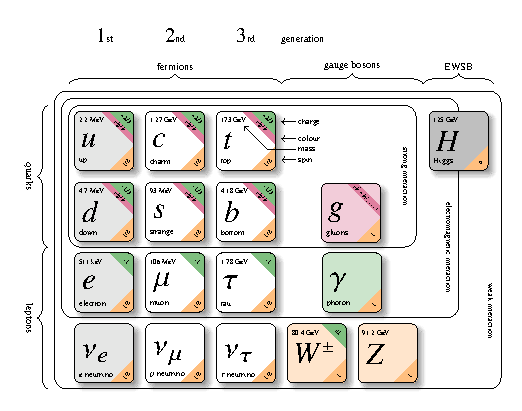
\includegraphics[width=\textwidth]{theory/sm}

  \caption{Particles of the SM. The diagram is adapted from Ref.~\Cref{sm_tikz}
    with updated particle properties from Ref.~X. Antiparticles are not shown
    explicitly have additive quantum numbers of opposite sign but otherwise the
    same properties of the respective particle.}
  \label{fig:sm_particles}
\end{figure}


The elementary particles of the SM can be divided into three categories:
\begin{description}

\item[Fermions] predicted by the SM have spin-$\frac{1}{2}$. Consequently, they
  are massive\footnote{Neutrinos are considered as massless in the SM, however,
    the observation of neutrino
    oscillations~\cite{Super-Kamiokande:1998kpq,SNO:2002tuh} is experimental
    evidence for neutrinos having small but non-zero mass.} and adhere to the
  Pauli exclusion principle and are therefore considered to be \emph{matter}
  particles. The fermions of the SM are divided into \emph{quarks} that take
  part in the strong interaction, and \emph{leptons} that do not.

  Divided into six \emph{flavours}???

  Up-type ($u$, $c$, $t$) and down-type ($d$, $s$, $b$) quarks.

  All fermions take part in the weak interactions while only quarks and
  electrically charged leptons ($e$, $\mu$, $\tau$) take part in the
  electromagnetic interaction. For every fermion, a corresponding anti-particle
  exists that has the same properties but with opposite additive quantum
  numbers.


  % All ordinary (stable) matter consists of fermions of the first generation,
  % i.e.\ up- and down-quarks as well as electrons. The only difference between
  % fermions of different generations is their mass.

  Quantum numbers: colour charge, electric charge, weak isospin (weak hypercharge)

\item[Gauge bosons] predicted by the SM are particles with spin-$1$ and are
  therefore also referred to as vector bosons. The gauge bosons mediate the
  three of the fundamental forces of nature. The strong interaction is mediate
  by the exchange of massless gluons that couple to colour charge carried by
  quarks and gluons. The massless photon couples to electric charge and thereby
  mediates the electromagnetic interaction. Finally, the massive $W^\pm$ and $Z$
  boson

\item[The Higgs boson]

\end{description}


Four types of vector (spin-1) bosons in.

The vector bosons mediate the fundamental interactions.

(Eight) gluons mediate the strong interaction.

The photon mediates the electromagnetic interaction.

The massive vector bosons $W^\pm$ and $Z$ mediate the weak interaction.

The mediators arise from theories adhering to certaing symmetry principles,
referred to as gauge theories, are therefore also referred to as \emph{gauge
  bosons}. A more detailed description of the interactions follows...

A special role in the SM is taken by the Higgs boson, the only scalar (spin-0)
boson in the SM. The Higgs boson is necessary to allow the $W^\pm$ and $Z$
bosons to be massive without violating the underlying symmetry principles of the
SM.

Bosons:

One scalar Boson, the Higgs boson. Explaining the mass of the heavy gauge bosons
without violating the symmetry assumptions underlying the Standard Model (more
on this later) using the BEH-mechanism.


Daily matter: electrons, up- and down-quarks.


In the SM the neutrinos are assumed to be mass-less which is experimentally
proven to not be the case.


\section{Symmetries and Interactions}

Guiding principle of the SM: local gauge invariance.


\subsection{The Langrange Formalism}

The description of the Standard Model uses the Lagrange formalism describing the
behaviour of fields, $\phi_i(\myvec{x})$, with a \emph{Lagrangian density}
$\lagrange(\phi_i, \partial_\mu \phi_i)$, where $\partial_\mu$ is the derivative
with respect to the $\mu$-th space-time coordinate. Hereafter, the Lagragian
density is referred to as the Lagrangian.

The ``equations of motion'' for the fields are obtained by the principle of
least action yielding Euler--Lagrange equations:
\begin{align*}
  \partial_{\mu} \left( \frac{\partial \lagrange}{\partial (\partial_{\mu} \phi_i)} \right) - \frac{\partial \lagrange}{\partial \phi_i} = 0
\end{align*}

$\partial_{\mu}$ is the covariant derivative $\partial / \partial x^{\mu}$.




\subsection{Local Gauge Invariance}

Interactions are dictated by symmetry principles


Symmetry group of the SM:
\begin{align*}
  SU(3)_{\text{color}} \times SU(2)_{\text{L}} \times U(1)_{Y}
\end{align*}

Lie group:
\begin{align*}
  U(\myvec{\alpha}) = \exp(i \myvec{\alpha} \cdot \myvec{G})
\end{align*}
U unitary. G generator (hermitian).


Local gauge invariance:
$\psi(\myvec{x}) \to \psi^\prime(\myvec{x}) = U(\myvec{x}) \psi(\myvec{x})$


\subsection{QED}

\begin{align*}
  \lagrange_{\text{Dirac}} = i \bar{\psi} \gamma^{\mu} \partial_{\mu} \psi - m \bar{\psi} \psi \quad \to \quad (i \gamma^{\mu} \partial_{\mu} - m) \psi = 0
\end{align*}

Dirac equation describing free fermions.

Perform local U(1) phase transformation.

The Dirac equation of a free fermion does not satisfy local gauge invariance due
to derivative terms.

Can introduce an alternative derivative: $D_\mu = \partial_\mu + i q A_\mu$.

Dirac spinor: $\psi$.


\subsection{QCD}

\subsection{Weak}

charged-current interaction $SU(2)$ symmetry -> weak isospin

Left handed chiral particles are in a weak isospin doublet

Right handed chiral particles are in a weak isospin singlett

Vice versa for antiparticles


\subsection{Electroweak Unification}

\section{Electroweak Symmetry Breaking}

\section{Fermion Masses}

\section{The Higgs Boson}


\clearpage

%%% Local Variables:
%%% mode: latex
%%% TeX-master: "../../phd_thesis"
%%% End:

\section{Particles of the Standard Model}%
\label{sec:sm_overview}

The SM, illustrated in~\Cref{fig:sm_particles}, consists of 12 elementary
spin-$\frac{1}{2}$ particles referred to as \emph{fermions} and their
antiparticles, and five types of particles with integer spin referred to as
\emph{bosons}. With the discovery of the Higgs boson in
2012~\cite{HIGG-2012-27,CMS-HIG-12-028}, experimental evidence for the existence
of all particles predicted by the SM is established.

\begin{figure}[htbp]
  \centering

  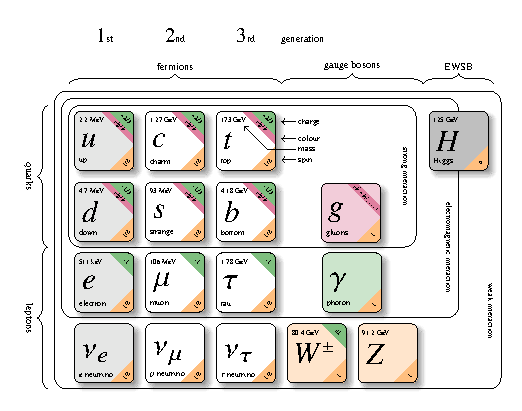
\includegraphics[width=\textwidth]{theory/sm}

  \caption{Particles of the SM. The diagram is adapted from Ref.~\cite{sm_tikz}
    with particle masses from Ref.~\cite{pdg2020}. Antifermions are not shown
    explicitly.  Not shown are the charges of the electroweak interaction, the
    weak isospin and weak hypercharge, which depend on the chirality of
    fermions. $*$: The gluons come in eight different states of colour charge
    which are combinations of colour and anticolour.}%
  \label{fig:sm_particles}
\end{figure}

An overview of the main categories of particles predicted by the SM is given in
the following:
\begin{description}

\item[Fermions] are massive\footnote{Neutrinos are considered as massless in the
    SM, however, the observation of neutrino
    oscillations~\cite{Super-Kamiokande:1998kpq,SNO:2002tuh} is experimental
    evidence for neutrinos having small but non-zero mass.} particles adhering
  to the Pauli exclusion principle. Therefore, they are often referred to as
  \emph{matter} particles. For every fermion there exists a corresponding
  antifermion that has the same properties but with additive quantum numbers of
  opposite sign. The fermions of the SM are divided into \emph{quarks} that
  participate in the strong interaction, and \emph{leptons} that do not. They
  are further divided into up-type quarks ($u$, $c$, $t$), down-type quarks
  ($d$, $s$, $b$), electrically charged leptons ($e$, $\mu$, $\tau$), and
  neutrinos ($\nu_e$, $\nu_\mu$, $\nu_\tau$). The fermions come in three
  generations, the main difference between them being the mass of the fermions
  which increases with every successive generation. Consequently, all ordinary
  (stable) matter consists of fermions of the first generation: up-quarks,
  down-quarks, and electrons.

  The fermions carry charge-like quantum numbers that dictate the fundamental
  interactions they take part in. Quarks carry \emph{colour charge}, which comes
  in three discrete values of either \emph{red}, \emph{green}, or \emph{blue},
  and the corresponding anticolours for antiquarks. Particles carrying colour
  charge take part in the strong interaction. Quarks and (electrically) charged
  leptons carry \emph{electric charge} and are therefore subject to the
  electromagnetic interaction. Fermions (antifermions) with left-handed
  (right-handed) chirality carry \emph{weak isospin}, therefore taking part in
  charged-current weak interactions. All fermions of the SM couple to the
  neutral-current weak interaction, the strength being determined by the weak
  isospin and the \emph{weak hypercharge} (or analogously the weak isospin and
  the electric charge, cf.~\Cref{seq:theory_ewk}).

\item[Gauge bosons] are particles with spin-$1$ and are therefore also referred
  to as vector bosons. Gauge bosons are the quanta of fields arising in quantum
  field theories built on certain symmetry principles, referred to as gauge
  theories, which will discussed in \Cref{sec:theo_symmetries_interactions}. The
  gauge bosons mediate strong, electromagnetic, and weak interaction through
  particle exchange.

  The (massless) gluons mediate the strong interaction through gluon exchange
  between particles with colour charge. Gluons are carriers of colour charge
  themselves, allowing self-interactions between gluons. The (massless) photon
  mediates the electromagnetic interaction between electrically charged
  particles. The gauge bosons of the weak interaction, the $W^\pm$ and $Z$
  bosons, are the only massive gauge bosons in the SM. The $W$ bosons are
  electrically charged and mediate the charged-current weak interaction between
  particles carrying weak isospin. The neutral $Z$ boson mediates the
  neutral-current weak interaction.

\item[The Higgs boson] is the only scalar particle (spin-$0$ and positive
  parity) in the SM. The Higgs boson arises as part of the Brout--Englert--Higgs
  (BEH) mechanism~\cite{Englert:1964et,Higgs:1964pj} that is employed in the SM
  to generate the masses of fermions and massive gauge bosons ($W^\pm$ and $Z$)
  without violating the symmetry principles underlying the mathematical
  formulation of the SM. The Higgs boson and its role in the SM is discussed in
  \Cref{seq:theory_ewk}.

\end{description}

%%% Local Variables:
%%% mode: latex
%%% TeX-master: "../../phd_thesis"
%%% End:

\section{Symmetries and Interactions}%
\label{sec:theo_symmetries_interactions}

The SM is a relativistic quantum field theory which describes particles and
their interaction using space-time dependent fields $\phi_i(\myvec{x})$. The
field dynamics are determined by the \emph{Lagrangian density} $\lagrange$,
which is a function of the fields $\phi_i$ and their space-time derivatives
$\partial_\mu \phi_i = \partial \phi_i / \partial x^\mu$ ($\mu = 0, 1, 2,
3$). The evolution of the fields in time follows from the principle of
stationary action, i.e.\ by extremising the action
$S = \int \mathrm{d}^4x \, \lagrange(\phi_i, \partial_\mu \phi_i)$, which yields
the Euler--Lagrange equations
\begin{align*}
  \partial_{\mu} \left( \frac{\partial \lagrange}{\partial (\partial_{\mu} \phi_i)} \right) - \frac{\partial \lagrange}{\partial \phi_i} = 0 \,\text{.}
\end{align*}
For a given Lagrangian, the Euler--Lagrange equations provide the ``equations of
motion'' of the fields. The Lagrangian density is hereafter simply referred to
as the \emph{Lagrangian}.

A continuous transformation of the fields that leaves the Lagrangian unchanged
is referred to as a \emph{gauge transformation}. The fields resulting from this
transformation follow the same equations of motion and therefore describe the
same physical system. This invariance is referred to as \emph{gauge invariance}
or \emph{gauge symmetry}.
% An external observer cannot distinguish between fields related by gauge
% transformations and therefore the symmetry is considered an \emph{internal
% symmetry} of the theory.
Continuous symmetries of the Lagrangian are characterised by Lie groups, the
most important ones for the description of the SM being the unitary group
$U(1)$, and the special unitary groups $SU(2)$ and $SU(3)$. Any element of a
unitary group can be written as
\begin{align*}
  \hat{U} = \exp\big[ i \theta_a G^a \big] \,\text{,}
\end{align*}
where $\theta_a$ are real parameters, and $G^a$ are the generators of the group.
% , and summation over repeated indices is implied.
A Lagrangian that is invariant to a transformation $\hat{U}$ of the fields with
parameters $\theta_a$ is said to possess \emph{global} gauge invariance. The
more restrictive case where the Lagrangian is invariant with respect to
transformations of the fields with space-time dependent parameters
$\theta_a(\myvec{x})$ is referred to as \emph{local} gauge invariance.

This is illustrated in the case of the Lagrangian of the Dirac field of mass $m$
given by
\begin{align}
  \lagrange_{\text{Dirac}} = \bar{\psi} (i \gamma^\mu  \partial_\mu - m) \psi \,\text{,}
  \label{eq:dirac_lagrangian}
\end{align}
where $\psi$ ($\bar{\psi} = \psi^\dagger \gamma^0$) are (adjoint) Dirac spinors,
and $\gamma^\mu$ are the Dirac matrices. \Cref{eq:dirac_lagrangian} possesses
global gauge invariance with respect to $U(1)$ transformations given by
$\psi \to \psi^\prime = \exp[ i q \theta ] \psi$, where $q$ is an arbitrary
constant (for the moment). However, when performing a local transformation by
letting the parameter be a function of space-time, i.e.\
$\theta \to \theta(\myvec{x})$, the invariance of the Lagrangian is spoiled due
to the derivative acting on the space-time dependent phase factor. One might
impose $U(1)$ local gauge invariance on the Lagrangian by adding terms to
\Cref{eq:dirac_lagrangian} that cancel the additional
contributions. Conventionally, this is done by substituting the derivative
$\partial_\mu$ by a gauge covariant derivative $D_\mu$ that transforms as
$D_\mu\psi \to \exp[ i q \theta(\myvec{x}) ] D_\mu\psi$, thus recovering local
gauge invariance. A definition of $D_\mu$ with these properties requires the
introduction of a new massless vector field, referred to as a \emph{gauge
  field}, with appropriate transformation properties:
\begin{align}
  D_\mu = \partial_\mu + i q A_\mu \qquad \text{with} \qquad A_\mu \xrightarrow{U(1)} A_\mu^\prime = A_\mu - \partial_\mu \theta(\myvec{x}) \,\text{.}
  \label{eq:covariant_derivative_qed}
\end{align}
The additional term introduced by substituting $\partial_\mu \to D_\mu$ in
\Cref{eq:dirac_lagrangian} is interpreted as an interaction between fermions and
vector bosons of the gauge field.

The principle of local gauge invariance can be used to obtain the Lagrangian of
quantum electrodynamics (QED) describing electromagnetic interactions. The
symmetry group of QED is $U(1)_{Q}$, the subscript $Q$ indicating that the
generator of the group is the electric charge operator. Imposing local gauge
invariance by substituting \Cref{eq:covariant_derivative_qed} into the Dirac
Lagrangian yields the interaction term
\begin{align*}
  \lagrange_{\text{int.}} = - q \bar{\psi} \gamma^\mu \psi A_\mu \,\text{.}
\end{align*}
In the case of QED, the field $A^\mu$ is identified as the four-potential of the
electromagnetic field, and $q$ as the electric charge of the fermion.
% The interaction term that was included to perserve local gauge invariance corresponds
Thus, the interaction term describes the coupling between photons and fermions
with electric charge $q$. For a single type of fermion, the Lagrangian of QED is
given by
\begin{align*}
  \lagrange_{\text{QED}} = \underbrace{\lagrange_{\text{Dirac}}}_{\text{Free fermion field}}
  \hspace*{1em}
  \underbrace{- q \bar{\psi} \gamma^\mu \psi A_\mu}_{\text{Fermion--photon interaction}}
  \hspace*{1em}
  \underbrace{- \frac{1}{4} F_{\mu\nu} F^{\mu\nu}}_{\text{Photon field kinetic term}} \,\text{,}
\end{align*}
which additionally includes the Lagrangian of the free photon field, referred to
as the \emph{kinetic term} of the field, defined by the electromagnetic tensor
$F_{\mu\nu} = \partial_\mu A_\nu - \partial_\nu A_\mu$. This additional term
also fulfils the local gauge invariance with respect to $U(1)_Q$.

The principle of local gauge invariance is at the heart of the SM where it is
used to great success in describing the three fundamental interactions. The
symmetry group of the SM is
\begin{align*}
  SU(3)_{\text{colour}} \otimes SU(2)_{\text{L}} \otimes U(1)_Y \,\text{,}
\end{align*}
where $SU(3)_{\text{colour}}$ is the symmetry of the strong interaction, and
$SU(2)_{\text{L}} \otimes U(1)_Y$ the symmetry of the unified description of the
electromagnetic and weak interaction. These will be introduced in
\Cref{sec:theory_qcd} and \Cref{seq:theory_ewk}, respectively.


\subsection{Quantum Chromodynamics}%
\label{sec:theory_qcd}

Quantum chromodynamics (QCD) is the theory describing the interactions of quarks
and gluons. The fundamental charge of QCD is colour charge which comes in three
distinct colours referred to as red, green, and blue (r, g, b). The quark fields
are consequently written in terms of the three component objects
\begin{align*}
  \psi =
  \begin{pmatrix}
    q_\text{r} \\
    q_\text{g} \\
    q_\text{b}
  \end{pmatrix}
  \qquad
  \text{and}
  \qquad
  \bar{\psi} =
  \begin{pmatrix}
    \bar{q}_\text{r} & \bar{q}_\text{g} & \bar{q}_\text{b}
  \end{pmatrix} \,\text{,}
\end{align*}
in which $q_i$ ($\bar{q}_i$) represents the (adjoint) Dirac spinor describing
the quark field with colour $i$. The symmetry group of the strong interaction is
$SU(3)_{\text{colour}}$, the subscript indicating that elements of the group act
in colour-space. The generators of $SU(3)_{\text{colour}}$ are taken to be
\begin{align*}
  T_a = \frac{1}{2} \lambda_a \qquad \text{for} \qquad a = 1, \dots, 8 \,\text{,}
\end{align*}
where $\lambda_a$ are the Gell-Mann matrices.\footnote{Mathematical objects with
  an upper Latin index and those with a lower Latin index are assumed to be
  equivalent.} The theory of QCD is referred to as a Yang--Mills gauge
theory~\cite{Yang:1954ek} since the elements of $SU(3)_{\text{colour}}$ do not
commute in general, i.e.\ the symmetry group is non-Abelian. The commutation
relation between the generators is given by $[T_a, T_b] = i f_{abc} T^c$,
defining the structure constants $f_{abc}$ of the group.

The principle of local gauge invariance with respect to $SU(3)_{\text{colour}}$
is used to obtain the Lagrangian of QCD. Let the local gauge transformation of
the quark fields be
\begin{align*}
  \psi \to \psi^\prime = \exp[ i g_{\text{s}} \theta_a(\myvec{x}) T^a] \psi \,\text{,}
  %\qquad
  %\bar{\psi} \to \bar{\psi}^\prime = \bar{\psi} \exp[ - i g_{\text{s}} \theta_a(\myvec{x}) T^a]  \,\text{,}
\end{align*}
where $g_{\text{s}}$ is referred to as the strong coupling constant. The gauge
covariant derivative is then
\begin{align*}
  D_\mu = \partial_\mu + i g_{\text{s}} G_\mu^a T_a \,\text{,}
  %\qquad \text{with} \qquad
  %G_\mu^k \xrightarrow{SU(3)_{\text{colour}}} {G_\mu^k}^\prime = G_\mu^k  - \partial_\mu \theta^k(\myvec{x}) - g_{\text{s}} {f_{ij}}^k \theta^i(\myvec{x}) G_\mu^j \,\text{,}
\end{align*}
which introduces eight gauge fields $G_\mu^a$ corresponding to the eight gluons
of QCD. To ensure local gauge invariance, the gluon fields have to transform
according to
\begin{align*}
  G_\mu^k \xrightarrow{SU(3)_{\text{colour}}} {G_\mu^k}^\prime = G_\mu^k  - \partial_\mu \theta^k(\myvec{x}) - g_{\text{s}} {f_{ij}}^k \theta^i(\myvec{x}) G_\mu^j \,\text{.}
\end{align*}
Furthermore, the Lagrangian of QCD has to account for the energy density of the
gluon fields (and their interactions). This contribution is given by the kinetic
term of the gluon fields and reads
\begin{align*}
  \lagrange_{g} = - \frac{1}{4} G_{\mu\nu}^{a} G^{\mu\nu}_{a} \,\text{,}
\end{align*}
where $G_{\mu\nu}^a$ are the gluon field strength tensors defined as
\begin{align*}
  G_{\mu\nu}^a = \partial_\mu G_\nu^a - \partial_\nu G_\mu^a - g_{\text{s}} {f^{a}}_{bc} G_\mu^b G_\nu ^c \,\text{.}
\end{align*}
The Lagrangian of QCD for a single flavour of quark with mass $m$ is
consequently given by
\begin{align*}
  \lagrange_{\text{QCD}} =
  \underbrace{\bar{\psi} (i \gamma^\mu \partial_\mu - m) \psi}_{\text{Free quark field}}
  \hspace*{1em}
  \underbrace{- g_{\text{s}} (\bar{\psi} \gamma^\mu T_a \psi) G_\mu^a}_{\text{Quark--gluon interactions}}
  \hspace*{1em}
  \underbrace{- \frac{1}{4} G_{\mu\nu}^a G^{\mu\nu}_a}_{\text{Gluon field kinetic term}} \,\text{.}
  %\label{eq:qcd_lagrangian}
\end{align*}
This Lagrangian describes the free quark field, the interactions of quarks with
the eight gluons, and the kinetic energy of the gluon fields. The non-Abelian
nature of the $SU(3)_{\text{colour}}$ group, meaning a set of indices exists
such that $f_{abc} \neq 0$, gives rise to the distinct structure of QCD through
the kinetic term of the gluon fields. This term includes self-interactions
between gluons which correspond to, in the language of Feynman diagrams, triple
and quartic interaction vertices between gluons. Gluons themselves are carriers
of colour charge which leads to this behaviour. This is unlike the photon of QED
which does not carry electrical charge and thus does not couple to itself.

Two important features of the theory of QCD are highlighted in the following:
\begin{description}

\item[Colour confinement] Due to the dynamics of the gluon self-interactions,
  free quarks or gluons cannot be observed in nature~\cite{Wilson:1974sk}. For
  example, separating the quarks of a quark-antiquark pair leads to the
  formation of \emph{flux tubes} in the gluon field strength that result in a
  linear increase in field energy with separation of the quarks. Eventually, the
  energy stored in the gluon field is sufficiently large to create a
  quark-antiquark pair from the vacuum. This process repeats until only quarks
  or gluons bound into colourless composite particles (colour singlet states)
  remain. The most prevalent bound states of quarks are (anti-)baryons
  consisting of three (anti-)quarks, and mesons consisting of a quark-antiquark
  pair. The $SU(3)_{\text{colour}}$ symmetry also allows for colour singlet
  states of multiple gluons referred to as
  \emph{glueballs}~\cite{Fritzsch:1972jv,Fritzsch:1975tx}, or other combinations
  of quarks such as tetra- ($q_1 \bar{q}_2 q_3 \bar{q}_4$) or pentaquarks
  ($q_1 q_2 q_3 q_4 \bar{q}_5$)~\cite{Gell-Mann:1964ewy}.

\item[Running coupling \& asymptotic freedom] The strong coupling constant,
  frequently expressed as $\alphas = g_{\text{s}}^2 / (4 \pi)$ in analogy to the
  fine-structure constant $\alpha = e^2 / (4 \pi)$ of QED, is not constant but
  varies as a function of the momentum transfer $Q$ of an interaction. A quark
  scattering process involving the exchange of a gluon is represented by an
  infinite number of Feynman diagrams with different higher-order corrections,
  for example diagrams with additional quark or gluon loops. A process referred
  to as \emph{renormalisation} absorbs these corrections into an effective
  coupling constant, the coupling consequently becoming a function of
  $Q^2$. This effect occurs in both QED and QCD, however, with distinct
  signatures. While the coupling $\alpha(Q^2)$ of QED increases with $Q^2$,
  $\alphas(Q^2)$ of QCD decreases with $Q^2$ due to gluon self-interactions. The
  high-$Q^2$ behaviour of \alphas is referred to as \emph{asymptotic
    freedom}~\cite{Gross:1973id,Politzer:1973fx}.
  % At large $Q^2$ the value of \alphas is small such that perturbative methods
  % can be used to obtain cross section predictions.
\end{description}


\subsection{Theory of the Electroweak Interaction}%
\label{seq:theory_ewk}

The principle of local gauge invariance was previously used to obtain the
Lagrangians of QED and QCD. The characteristics of the weak interaction make
this approach more difficult. First, the mediators of the interaction are
massive with masses of ~\cite{pdg2020}
\begin{align*}
  m_W = \SI{80.377 +- 0.012}{\GeV}
  \qquad \text{and} \qquad
  m_{Z} = \SI{91.1876 +- 0.0021}{\GeV} \text{.}
\end{align*}
Second, the symmetry with respect to parity (space-inversion) transformations is
violated~\cite{Wu:1957my}. Lastly, the charged-current weak interaction couples
fermions of different flavour that differ by one unit in electric charge. Due to
these characteristics, the construction of a gauge theory of the weak
interaction that respects local gauge invariance requires the introduction of
new mechanisms.
% that were not needed for the description of QED and QCD.

\subsubsection{Electroweak Unification}

The theory of the electroweak interaction was developed by Glashow, Salam, and
Weinberg in the 1960s to unify the electromagnetic and weak interactions in a
single model~\cite{Glashow:1961tr,Salam:1964ry,Weinberg:1967tq}. The theory is
constructed as a non-Abelian gauge theory based on a symmetry group referred to
as $SU(2)_{\text{L}} \otimes U(1)_{Y}$, the meaning of the subscripts will be
illustrated in the following.

First, a new quantum number referred to as \emph{weak isospin} denoted by $I$,
and its component along the 3-axis, $I_3$, is introduced. The charged-current
weak interaction violates parity symmetry maximally, meaning it only couples to
fermionic fields with left-handed chirality.\footnote{Chirality of a Dirac field
  is defined by the operator
  $\gamma^5 \coloneq i \gamma^0 \gamma^1 \gamma^2 \gamma^3$. The eigenvectors of
  $\gamma^5$ are states of well-defined chirality with eigenvalues of $+1$ or
  $-1$, referred to as right- and left-handed chiral states, respectively. Any
  spinor can be written as a superposition of right- and left-handed chiral
  states using the projection operators
  $P_{\text{R/L}} = (1 \pm \gamma^5) / 2$.} An appropriate weak isospin grouping
of SM fermions is chosen in anticipation of a $SU(2)$ symmetry.
% Based on the experimental observation that the charged-current weak
% interaction only couples to particles (antiparticles) with left-handed
% (right-handed) chirality, an appropriate grouping of the SM fermions is
% chosen.
Left-handed fermion fields are grouped into weak isospin doublets given by
\begin{align*}
  \begin{pmatrix}
    \nu_{e} \\
    e^{-}
  \end{pmatrix}_{\text{L}},
  \begin{pmatrix}
    \nu_{\mu} \\
    \mu^{-}
  \end{pmatrix}_{\text{L}},
  \begin{pmatrix}
    \nu_{\tau} \\
    \tau^{-}
  \end{pmatrix}_{\text{L}}
  \qquad
  \begin{pmatrix}
    u \\
    d
  \end{pmatrix}_{\text{L}},
  \begin{pmatrix}
    c \\
    s
  \end{pmatrix}_{\text{L}},
  \begin{pmatrix}
    t \\
    b
  \end{pmatrix}_{\text{L}}
  \qquad
  \text{with}
  \qquad
  I = \frac{1}{2}, I_3 = \pm \frac{1}{2} \,\text{,}
\end{align*}
where the upper (lower) components correspond to $I_3 = +\frac{1}{2}$
($I_3 = -\frac{1}{2}$), and nine singlet states for right-handed fermion fields
\begin{align*}
  e^{-}_{\text{R}}, \mu^{-}_{\text{R}}, \tau^{-}_{\text{R}},
  u_{\text{R}}, d_{\text{R}}, c_{\text{R}}, s_{\text{R}}, t_{\text{R}}, b_{\text{R}}
  \qquad
  \text{with}
  \qquad
  I = 0, I_3 = 0 \,\text{,}
\end{align*}
where the subscripts L and R refer to the projection of the fields into their
left- and right-handed chiral components,
respectively. % The quark eigenstates of
% the weak interaction are indicated by $d^\prime, s^\prime, b^\prime$ which are
% related to the quark mass eigenstates via the Cabibbo--Kobayashi--Maskawa
% matrix~\cite{Cabibbo:1963yz,Kobayashi:1973fv}.
Right-handed neutrinos are omitted since they are not part of the SM.
% \footnote{The determination of the nature of neutrinos is still an active area
% of physics research. In the SM, neutrinos are assumed to be massless which is
% in disagreement with the observation of neutrino oscillations. Under the
% assumption that neutrinos are Dirac particles, the non-vanishing mass would
% suggest that there is mixing between left- and right-handed chiral states of
% neutrinos. However, in the current theory right-handed neutrinos would be
% ``sterile'' meaning they would not interact via any of the interactions
% described by the SM. Alternative proposals are that neutrinos are not Dirac
% but Majorana particles~\cite{Majorana:1937vz}, which are particles that are
% identical to their antiparticles.}
Given this grouping, $SU(2)_{\text{L}}$ transformations only affect fermion
fields with left-handed chirality, thus motivating the choice of subscript.
% \todo{If we are assuming massless quarks -> mass and weak eigenstates are the
% same.}

Second, a quantum number referred to as the \emph{weak hypercharge} is defined
according to
\begin{align*}
  Y = 2 (Q - I_3) \,\text{,}
\end{align*}
where $Q$ refers to the electric charge. Since the electric charge differs
between the upper and lower component of the $SU(2)_{\text{L}}$ doublets, a
$SU(2)_{\text{L}}$ transformation would violate the $U(1)_Q$ symmetry of
QED. Therefore, the weak hypercharge is defined such that both components of a
$SU(2)_{\text{L}}$ doublet have the same value of $Y$. The broken $U(1)_Q$
symmetry is consequently replaced by a $U(1)_Y$ symmetry, which uses $Y$ as the
generator of the group instead. The $U(1)_Q$ symmetry of QED will later be
recovered in a process referred to as \emph{electroweak symmetry breaking}
(EWSB).

The principle of local gauge invariance with respect to the
$SU(2)_{\text{L}} \otimes U(1)_Y$ group is invoked to generate the interactions
of the electroweak theory. In the following, the weak isospin doublets are
denoted as $\chi_{\text{L}}$ and weak isospin singlets as $\psi_{\text{R}}$. The
gauge transformations with space-time dependent parameters $\alpha_a$
($a = 1, 2, 3$) and $\beta$ transform the fields as follows
\begin{align*}
  &\chi_{\text{L}} \to \chi_{\text{L}}^\prime = \exp\left[ i g \alpha_a(\myvec{x}) \frac{\sigma^a}{2} + i g^\prime \beta(\myvec{x}) \frac{Y}{2} \right] \chi_{\text{L}} \\
  &\psi_{\text{R}} \to \psi_{\text{R}}^\prime = \exp\left[ i g^\prime \beta(\myvec{x}) \frac{Y}{2} \right] \psi_{\text{R}} \,\text{,}
\end{align*}
where $g$ and $g^\prime$ are coupling constants, and $\sigma^a$ are the Pauli
matrices. The gauge covariant derivative is given by
\begin{align*}
  D_\mu = \partial_\mu
  + i g W^a_\mu \frac{\sigma_a}{2}
  + i g^\prime B_\mu \frac{Y}{2} \,\text{,}
\end{align*}
where it is implied that the Pauli matrices only act on $\chi_{\text{L}}$ and
not on $\psi_{\text{R}}$. Four gauge fields, $W_\mu^a$ ($a = 1, 2, 3$) and
$B_\mu$, associated with the $SU(2)_{\text{L}}$ and $U(1)_Y$ symmetry are
introduced. These fields transform, in analogy to QED and QCD, as follows
\begin{align*}
  W_\mu^k &\xrightarrow{SU(2)_{\text{L}} \otimes SU(1)_Y} {W_\mu^k}^\prime = W_\mu^k - \partial_\mu \alpha^{k}(\myvec{x}) - g {f_{ij}}^k \alpha^{i} W_\mu^j \\
  B_\mu   &\xrightarrow{SU(2)_{\text{L}} \otimes SU(1)_Y} {B_\mu}^\prime = B_\mu - \partial_\mu \beta(\myvec{x}) \,\text{,}
\end{align*}
where $f_{ijk}$ are the structure constants of $SU(2)_{\text{L}}$ with the
generators of the group taken to be $\frac{1}{2} \sigma_a$.  Substituting the
gauge covariant derivative into the kinetic term of the Dirac Lagrangian yields
the interaction terms of the electroweak theory for left- and right-handed
chiral fields
\begin{align}
  &\lagrange_{\text{int.}}^{\text{L}} = i \bar{\chi}_{\text{L}} \gamma^\mu \left[i g W_\mu^a \frac{\sigma_a}{2} + i g^\prime B_\mu \frac{Y}{2} \right] \chi_{\text{L}} \label{eq:theory_electroweak_left} \\
  &\lagrange_{\text{int.}}^{\text{R}} = i \bar{\psi}_{\text{R}} \gamma^\mu \left[i g^\prime B_\mu \frac{Y}{2} \right] \psi_{\text{R}} \,\text{.} \label{eq:theory_electroweak_right}
\end{align}
The four fields occurring in the interaction terms do not represent the physical
fields observed in nature. Given the choice of Pauli matrices as the generators
of $SU(2)_{\text{L}}$, the fields $W_\mu^1$ and $W_\mu^2$ are associated with
charged-current interactions, and $W_\mu^3$ and $B_\mu$ with neutral-current
interactions. The physical fields of the charged-current interaction can be
identified as
\begin{align*}
  W_\mu^\pm = \frac{1}{\sqrt{2}} (W_\mu^1 \mp i W_\mu^2) \,\text{.}
\end{align*}
% in analogy to the weak isospin ladder operators.
Furthermore, the physical fields describing the neutral-current interactions via
the exchange of $Z$ bosons and photons can be expressed as a linear combination
of the $W_\mu^3$ and $B_\mu$ gauge fields. Experimental results show that the
$Z$ boson couples to both left- and right-handed chiral states, although not
equally, and therefore such a mixing is required. The mixing can be described by
a rotation of the fields by the weak mixing angle $\theta_{\text{W}}$ according
to
\begin{align*}
  \begin{pmatrix}
    A_\mu \\
    Z_\mu
  \end{pmatrix}
  =
  \begin{pmatrix}
    \cos\theta_{\text{W}} & \sin\theta_{\text{W}} \\
    -\sin\theta_{\text{W}} & \cos\theta_{\text{W}}
  \end{pmatrix}
  \begin{pmatrix}
    B_\mu \\
    W_\mu^3
  \end{pmatrix} \,\text{.}
\end{align*}
The weak mixing angle must be chosen such that
\Cref{eq:theory_electroweak_left,eq:theory_electroweak_right} reproduce the
coupling of QED, namely the photon must couple equally to left- and right-handed
particles with a coupling constant $e$. This yields the condition
\begin{align*}
  e = g \sin\theta_{\text{W}} = g^\prime \cos\theta_{\text{W}} \,\text{,}
\end{align*}
% \todo{Note ways to express sin / cos as a function of $g$ and $g^\prime$.}
connecting the QED coupling constant with the coupling constants $g$ and
$g^\prime$ of the electroweak interaction. Finally, the kinetic term of the
$W_\mu^a$ and $B_\mu$ fields is given, in analogy to QED and QCD, by
\begin{align*}
  \lagrange_{W, Z, \gamma} =
  - \frac{1}{4} W_{\mu\nu}^a W^{\mu\nu}_a
  - \frac{1}{4} B_{\mu\nu} B^{\mu\nu} \,\text{,}
\end{align*}
where the field strength tensors are defined as
\begin{align*}
  W_{\mu\nu}^a &= \partial_\mu W_\nu^a - \partial_\nu W_\mu^a - g {f^a}_{bc} W_\mu^b W_\nu^c \\
  B_{\mu\nu} &= \partial_\mu B_\nu - \partial_\nu B_\mu \,\text{.}
\end{align*}
Since $SU(2)_{\text{L}}$ is a non-Abelian group, triple and quartic gauge boson
couplings are introduced through the kinetic term of the $W_\mu^a$ fields.


\subsubsection{The Brout--Englert--Higgs Mechanism}

In the context of the electroweak theory, the non-zero masses of the gauge
bosons (and fermions) have been ignored thus far. Inserting gauge field mass
terms into the Lagrangian, for example for the physical $Z_\mu$ field with mass
$m_Z$ according to
\begin{align*}
  \lagrange_{\text{mass}}^{Z} = \frac{1}{2} m_{Z}^2 Z_\mu Z^\mu \,\text{,}
\end{align*}
would violate $SU(2)_{\text{L}} \otimes U(1)_Y$ symmetry due to the
transformation properties of the fields. A mechanism to dynamically generate the
required mass terms was introduced into the electroweak theory by
Weinberg~\cite{Weinberg:1967tq} to address this issue. This mechanism traces
back to Brout, Englert, and Higgs~\cite{Englert:1964et,Higgs:1964pj} and is thus
referred to as the Brout--Englert--Higgs (BEH) mechanism.

The BEH mechanism introduces two complex scalar fields, one electrically charged
and one neutral field, arranged in a weak isospin doublet with $Y = 1$ according
to
\begin{align*}
  \phi =
  \begin{pmatrix}
    \phi^+ \\
    \phi^0
  \end{pmatrix}
  = \frac{1}{\sqrt{2}}
  \begin{pmatrix}
    \phi_1 + i \phi_2 \\
    \phi_3 + i \phi_4
  \end{pmatrix} \,\text{,}
\end{align*}
which can analogously be expressed as four real scalar fields $\phi_i$. The
Lagrangian of the complex scalar fields is given by the Klein--Gordon equation
\begin{align*}
  \lagrange = (\partial_\mu \phi)^\dagger (\partial^\mu \phi) - V(\phi)
\end{align*}
with the potential term denoted by $V(\phi)$. The aim of the BEH mechanism is to
embed the doublet of complex scalar fields into the electroweak theory with a
$SU(2)_{\text{L}}\otimes U(1)_Y$ symmetry. To fulfil the gauge invariance of the
electroweak theory, the potential term can only depend on $\phi^\dagger
\phi$. One such choice is
\begin{align}
  V(\phi) = \mu^2 \phi^\dagger \phi + \lambda (\phi^\dagger \phi)^2
  \label{eq:higgs_potential}
\end{align}
with $\mu^2$ and $\lambda$ being parameters of the potential.\footnote{In terms
  of the renormalisability of the theory, the largest allowed power of
  $\phi^\dagger \phi$ in the Lagrangian is two. See for example
  Ref.~\cite{Peskin:1995ev}.} The potential must be bound from below to have a
well-defined state of minimum potential energy (vacuum state) and therefore
$\lambda$ must be positive. No such restrictions exist for $\mu^2$, leaving two
options. If $\mu^2 > 0$, the vacuum state is $\phi = \myvec{0}$ and $\mu$ is
related to the mass of the scalar field. If $\mu^2 < 0$, the field configuration
$\phi = \myvec{0}$ is at an unstable point and the true vacuum is given by the
condition
\begin{align*}
  \sum_{i = 1}^4 \phi_i^2 = -\frac{\mu^2}{\lambda} \eqqcolon \varv^2 \,\text{,}
\end{align*}
which represents a continuum of degenerate states at a radius of $\varv$ from the
origin in the space spanned by the four real scalar fields. The quantity $\varv$ is
therefore referred to as the \emph{vacuum expectation value} (VEV). Hereafter,
this particular choice of potential is referred to as the Higgs potential. This
choice is illustrated in \Cref{fig:mexican_hat} for a simplified model with only
a single complex scalar field.

\begin{figure}[htbp]
  \centering

  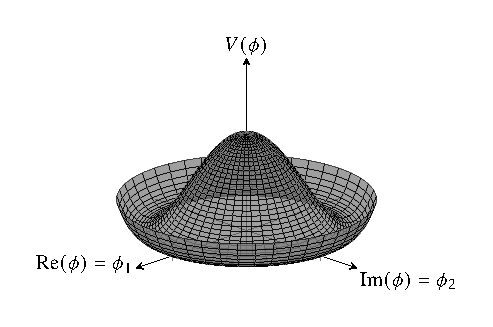
\includegraphics[scale=1.1]{theory/potential}

  \caption[The ``Mexican-hat potential'' of a complex scalar field.]{The
    ``Mexican-hat potential'' of a single complex scalar field as a low
    dimensional example to illustrate the choice of the Higgs potential in the
    SM. The degenerate vacuum states lie in a circle with radius $\varv$ given by
    the condition $\phi_1^2 + \phi_2^2 = \varv^2$. Adapted from
    Ref.~\cite{higgs_potential_tikz}.}%
  \label{fig:mexican_hat}
\end{figure}

The fields $\phi_i$ will assume a configuration that minimises the potential
energy, hence realising one of the infinite number of vacuum states. While the
full Lagrangian still possesses a $SU(2)_{\text{L}} \otimes U(1)_Y$ symmetry,
the spontaneous choice of a vacuum state with non-vanishing VEV appears to break
the symmetry, a process referred to as \emph{spontaneous symmetry
  breaking}. Perturbative methods are used to find solutions to the field
equations of motion, hence the fields have to be expressed as small
perturbations relative to the vacuum state. Let the vacuum state be
\begin{align*}
  \phi_{\text{v}} = \frac{1}{\sqrt{2}}
  \begin{pmatrix}
    0 \\
    \varv
  \end{pmatrix} \,\text{,}
\end{align*}
chosen such that only the neutral component is non-vanishing to ensure that the
$U(1)_Q$ symmetry of QED is recovered after spontaneous symmetry
breaking.\footnote{An infinitesimal $U(1)_Q$ transformation yields
  $(1 + i \epsilon Q) \phi_{\text{v}} = \phi_{\text{v}}$, thus leaving the
  vacuum state unchanged. This is not the case when replacing $Q$ with the
  generators of $SU(2)_{\text{L}}$ or $U(1)_Y$.} Four degrees of freedom for
perturbations relative to the chosen vacuum state exist. Three degrees of
freedom are chosen such that they leave $\phi^\dagger \phi$, and thus $V(\phi)$,
invariant. The remaining degree of freedom alters the value of
$\phi^\dagger \phi$ and therefore $V(\phi)$.\footnote{In the toy model depicted
  in \Cref{fig:mexican_hat}, the degrees of freedom correspond to perturbations
  of the vacuum state in angular and radial direction, respectively.} In the
Lagrangian describing the fields $\phi$, these perturbations appear as three
massless scalar fields and one massive scalar field. The quanta of the massless
fields are referred to as Nambu--Goldstone
bosons~\cite{Nambu:1960tm,Goldstone:1961eq}, however, a suitable gauge
transformation, referred to as the \emph{unitary gauge}, allows to remove the
massless scalar fields from the theory. In unitary gauge, the doublet of complex
scalar fields can be expressed as
\begin{align}
  \phi(\myvec{x}) = \frac{1}{\sqrt{2}}
  \begin{pmatrix}
    0 \\
    \varv + H(\myvec{x})
  \end{pmatrix}
  \label{eq:vacuum_state_perturb}
\end{align}
with $H(\myvec{x}) \in \mathbb{R}$.

% Check: https://arxiv.org/pdf/1704.02311.pdf
Expressing the Higgs potential of \Cref{eq:higgs_potential} in terms of
perturbations of the vacuum state, i.e.\ using \Cref{eq:vacuum_state_perturb},
and dropping terms not depending on $H$ yields
\begin{align}
  V(H) =
  \lambda \varv^2 H^2
  + \lambda \varv H^3
  + \frac{\lambda}{4} H^4 \,\text{.}
  \label{eq:beh_potential}
\end{align}
The first term of $V(H)$ represents the mass term of the scalar field $H$ with a
mass of $m_H = \sqrt{2\lambda} \varv$. The quantum of the scalar field is
referred to as the Higgs boson ($H$).\footnote{Depending on the context, $H$
  refers to the Higgs boson or the scalar field that describes the Higgs field
  in unitary gauge.} The terms cubic and quartic in the scalar field represent
self-interactions between Higgs bosons with coupling strengths defined
as\footnote{There exists no consensus regarding the definition of
  $\lambda_{HHH}$ and $\lambda_{HHHH}$. In this thesis a convention is adopted
  such that the Higgs potential can be expressed as
  \begin{align*}
    V(H) = \frac{m_{H}^2}{2} H^2 + \frac{\lambda_{HHH}}{3!} H^3 + \frac{\lambda_{HHHH}}{4!}
    H^4 \,\text{.}
  \end{align*}
}
\begin{align*}
  \lambda_{HHH} \coloneqq \frac{3 m_{H}^2}{\varv} \qquad \text{and} \qquad \lambda_{HHHH} \coloneqq \frac{3 m_{H}^2}{\varv^2} \,\text{.}
\end{align*}
The Feynman vertices of Higgs boson self-interactions are depicted in
\Cref{fig:vertex_hhh,fig:vertex_hhhh}.

The term of the Klein--Gordon equation involving the space-time derivatives
yield after substituting the $SU(2)_{\text{L}} \otimes U(1)_Y$ gauge covariant
derivative and inserting the physical fields describing the $W$ and $Z$ bosons
\begin{align}
  (D_\mu \phi)^\dagger (D^\mu \phi) =
  \frac{1}{2} (\partial_\mu H) (\partial^\mu H)
  + \left[
  \frac{g^2 \varv^2}{4} W^{-}_\mu {W^{+}}^\mu
  +
  \frac{(g^2 + {g^\prime}^2) \varv^2}{8} Z_\mu Z^\mu
  \right] \left( 1 + \frac{1}{\varv} H \right)^2 \,\text{.}
  \label{eq:higgs_covariant_derivative}
\end{align}
The first term of \Cref{eq:higgs_covariant_derivative} yields the kinetic term
for the scalar field $H$. Moreover, the BEH mechanism dynamically generates mass
terms for the $W^\pm$ and $Z$ bosons while leaving the photon massless. Using
the four parameters of the electroweak theory ($g$, $g^\prime$, $m_{H}$, $\varv$)
the masses of the bosons can be obtained from the Lagrangian such that
\begin{align*}
  &m_W = \frac{1}{2} g \varv  &&m_Z = \frac{1}{2} \sqrt{g^2 + {g^\prime}^2} \, \varv && m_{\text{photon}} = 0 \,\text{.}
\end{align*}
\Cref{eq:higgs_covariant_derivative} additionally describes interaction vertices
of the form $WWH$, $ZZH$, $WWHH$, and $ZZHH$, which are depicted in
\Cref{fig:higgs_vertices}.

\begin{figure}[htbp]
  \centering

  \begin{subfigure}{0.33\textwidth}
    \centering
    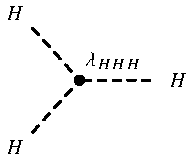
\includegraphics[scale=0.9]{feynman_graphs/higgs_hhh}
    \subcaption{}
    \label{fig:vertex_hhh}
  \end{subfigure}%
  \begin{subfigure}{0.33\textwidth}
    \centering
    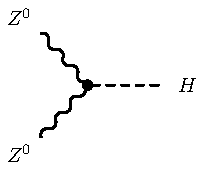
\includegraphics[scale=0.9]{feynman_graphs/higgs_hzz}
    \subcaption{}
  \end{subfigure}%
  \begin{subfigure}{0.33\textwidth}
    \centering
    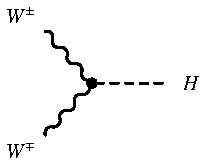
\includegraphics[scale=0.9]{feynman_graphs/higgs_hww}
    \subcaption{}
  \end{subfigure}

  \vspace{1em}

  \begin{subfigure}{0.33\textwidth}
    \centering
    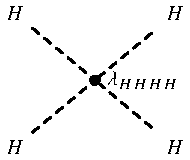
\includegraphics[scale=0.9]{feynman_graphs/higgs_hhhh}
    \subcaption{}
    \label{fig:vertex_hhhh}
  \end{subfigure}%
  \begin{subfigure}{0.33\textwidth}
    \centering
    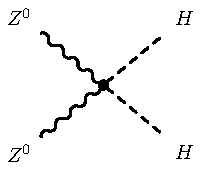
\includegraphics[scale=0.9]{feynman_graphs/higgs_hhzz}
    \subcaption{}
  \end{subfigure}%
  \begin{subfigure}{0.33\textwidth}
    \centering
    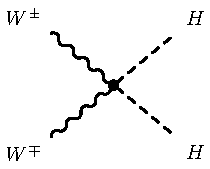
\includegraphics[scale=0.9]{feynman_graphs/higgs_hhww}
    \subcaption{}
  \end{subfigure}

  \caption[Interaction vertices between Higgs, $W$, and $Z$~bosons predicted by
  the SM.]{Interaction vertices between Higgs, $W$, and $Z$~bosons predicted by
    the SM.}%
  \label{fig:higgs_vertices}
\end{figure}

% Prior to the discovery of the Higgs boson, of the four parameters describing
% the electroweak theory the only one left to be determined was the mass of the
% Higgs boson, $m_{H}$. After the discovery of the Higgs boson and the
% measurement of its mass, no unknown parameters remain in the electroweak
% theory.

% Conventionally, the couplings of the electroweak unification are given in terms
% of $e$ and $\sin^2\theta_{\text{W}} = \num{0.23124 +- 0.00004}$ at
% $Q^2 = m_{Z}^2$~\cite{pdg2020}.


\subsubsection{Fermion Masses}

The inclusion of fermion mass terms of the form
\begin{align*}
  \lagrange_{\text{mass}}^{\text{fermion}} = - m \bar{\psi} \psi = - m [ \bar{\psi}_\text{R} \psi_\text{L} + \bar{\psi}_\text{L} \psi_\text{R} ]
\end{align*}
into the Lagrangian violates the gauge invariance with respect to the
$SU(2)_{\text{L}} \otimes U(1)_Y$ symmetry, since fermions with left- and
right-handed chirality transform differently. Instead, fermion mass terms are
generated dynamically through EWSB by introducing interactions between the
fermion fields and the scalar Higgs field, which are referred to as Yukawa
interactions~\cite{Yukawa:1935xg}.

First, the conjugate of the Higgs field $\phi$ is defined as
$\phi^{\text{c}} = i \sigma_2 \phi^*$, such that after after EWSB in unitary
gauge
\begin{align*}
  \phi^{\text{c}} = \frac{1}{\sqrt{2}}
  \begin{pmatrix}
    \varv + H(\myvec{x}) \\
    0
  \end{pmatrix} \,\text{.}
\end{align*}
A Lagrangian of the Yukawa interactions with $SU(2)_{\text{L}} \otimes U(1)_Y$
gauge invariance is defined, here exemplary for the first generation of
fermions, as
\begin{align}
  \lagrange_{\text{Yukawa}} =
  - y_e \bar{L} \phi e_{\text{R}}
  - y_u \bar{Q} \phi^{\text{c}} u_{\text{R}}
  - y_d \bar{Q} \phi d_{\text{R}}
  + \text{h.c.} \,\text{,}
  \label{eq:lagrangian_yukawa}
\end{align}
where $\bar{L}$ and $\bar{Q}$ are the $SU(2)_{\text{L}}$ doublets of the first
generation of leptons and quarks, respectively. The $SU(2)_{\text{L}}$ singlets
for electrons, up-, and down-quarks are denoted as $e_{\text{R}}$,
$u_{\text{R}}$, and $d_{\text{R}}$. Moreover, the coupling constants of the
Yukawa interactions, which are free parameters of the theory, are given by
$y_e$, $y_u$, and $y_d$. Finally, $\text{h.c.}$ represents the hermitian
conjugate of the preceding terms. After EWSB and in unitary gauge
\Cref{eq:lagrangian_yukawa} reads
\begin{align*}
  \lagrange_{\text{Yukawa}} \xrightarrow{\text{EWSB}} \sum_{f \in \{e, u, d\}} -\frac{y_{\hspace{-0.1em}f} \varv}{\sqrt{2}} [ \bar{f}_{\text{L}} f_{\text{R}} + \bar{f}_{\text{R}} f_{\text{L}} ] \left( 1 + \frac{1}{\varv} H \right)
\end{align*}
yielding fermion mass terms with masses
\begin{align*}
  m_{f} = \frac{y_{\hspace{-0.1em}f} \varv}{\sqrt{2}} \,\text{,}
\end{align*}
which are proportional to the Yukawa coupling constants, as well as interactions
between Higgs bosons and fermions with a coupling strength proportional to the
mass of the fermion given by
\begin{align*}
  g_{H\!f\!f} = \frac{m_f}{\varv} \,\text{.}
\end{align*}

The Lagrangian of \Cref{eq:lagrangian_yukawa} can be further generalised to
include the remaining fermion generations, and mixing between the weak and mass
eigenstates of quarks as described by the Cabibbo--Kobayashi--Maskawa
matrix~\cite{Cabibbo:1963yz,Kobayashi:1973fv}.


%%% Local Variables:
%%% mode: latex
%%% TeX-master: "../../phd_thesis"
%%% End:

\section{The Higgs Boson}

The Higgs boson



elementary particle


Discovery

ATLAS \cite{HIGG-2012-27} and CMS \cite{CMS-HIG-12-028}




\subsection{Production and Decay Modes}

\begin{figure}[htbp]
  \centering

  \begin{subfigure}{0.45\textwidth}
    \centering
    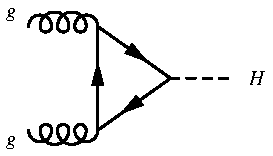
\includegraphics[scale=1]{feynman_graphs/higgs_prod_ggf}
    \subcaption{Gluon-gluon fusion (\ggF)}
  \end{subfigure}%
  \begin{subfigure}{0.45\textwidth}
    \centering
    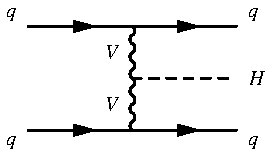
\includegraphics[scale=1]{feynman_graphs/higgs_prod_vbf}
    \subcaption{Vector boson fusion (VBF)}
  \end{subfigure}

  \begin{subfigure}{0.45\textwidth}
    \centering
    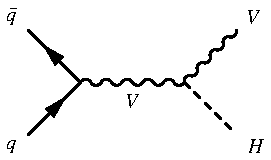
\includegraphics[scale=1]{feynman_graphs/higgs_prod_vh}
    \subcaption{Associated production with a vector boson ($VH$)}
  \end{subfigure}%
  \begin{subfigure}{0.45\textwidth}
    \centering
    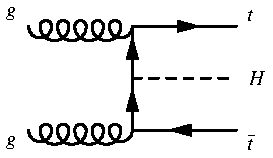
\includegraphics[scale=1]{feynman_graphs/higgs_prod_tth}
    \subcaption{Associated production with \ttbar ($\ttbar H$)}
  \end{subfigure}%

  \caption{The dominant Higgs boson production modes in \pp-collisions at
    centre-of-mass energies of \SI{13}{\TeV}.}
\end{figure}


Pair production of Higgs bosons is covered in detail in
\Cref{fig:theory_higgs_pair_prod}.



\subsection{Higgs Boson Pair Production}
\label{fig:theory_higgs_pair_prod}

Observation:






Production modes:

ggF, VBF, WH, ZH, ttH, (tH?)

HH

Decay modes:






Yukawa couplings:

To ``t''

To ``b''

To $\tau$

To $\mu$



\begin{figure}[htbp]
  \centering

  \begin{subfigure}[b]{0.47\textwidth}
    \centering

    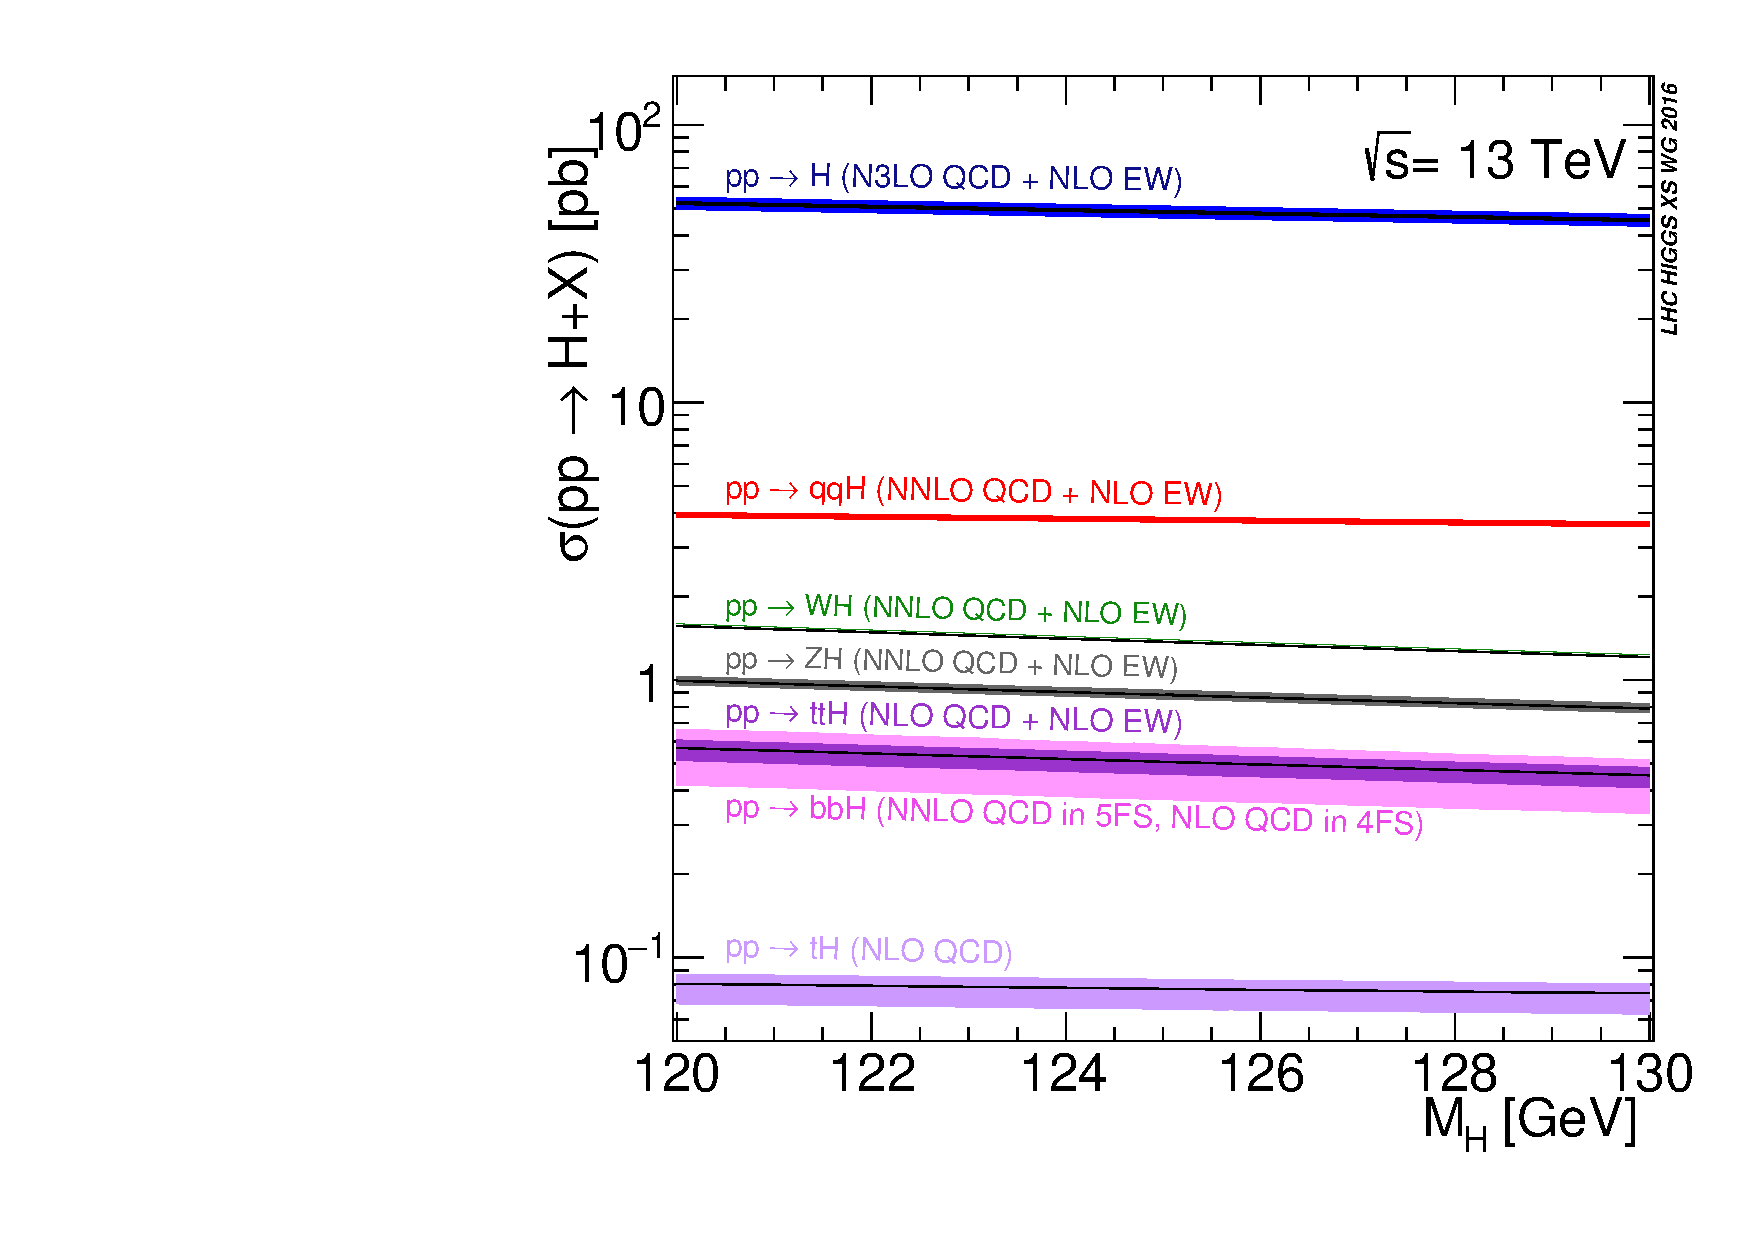
\includegraphics[width=0.95\textwidth]{theory/h_prod_crossec_13tev}

    \subcaption{Cross sections of Higgs boson production modes.}
  \end{subfigure}\hfill%
  \begin{subfigure}[b]{0.47\textwidth}
    \centering

    \renewcommand{\arraystretch}{1.1}%
    \begin{tabular}{lS[table-format=2.3]c}
  \toprule
  Decay mode  & {BR / \%} & Observed \\
  \midrule
  $\bbbar$        & 58    & \checkmark \\
  $W^{+} W^{-}$    & 21    & \checkmark \\
  $gg$            & 8.2   & \\
  $\tau^+ \tau^-$ & 6.3   & \checkmark \\
  $c\bar{c}$      & 2.9   & \\
  $ZZ^{*}$            & 2.6   & \checkmark \\
  $\gamma\gamma$  & 0.23  & \checkmark \\
  $Z\gamma$       & 0.15  & \\
  $\mu^{+}\mu^{-}$ & 0.022 & $\sim$~\cite{CMS-HIG-19-006} \\
  \bottomrule
\end{tabular}

%%% Local Variables:
%%% mode: latex
%%% TeX-master: "../phd_thesis"
%%% End:


    \subcaption{Branching ratios of Higgs boson decay modes. The $gg$,
      $\gamma\gamma$, and $Z\gamma$ decay modes occur via processes involving
      heavy quark loops.}
  \end{subfigure}

  \caption{Higgs boson production cross section in \pp-collisions at a
    centre-of-mass energy of \SI{13}{\TeV} (a) and Higgs boson decay branching
    ratios for $m_{H} = \SI{125.0}{\GeV}$ (b). The figure and branching ratios
    are taken from Ref.~\cite{deFlorian:2016spz}.}
\end{figure}


% \begin{figure}[htbp]
%   \centering

%   \begin{subfigure}{0.47\textwidth}
%     \centering

%     \subcaption{ATLAS $H \to ZZ$}
%   \end{subfigure}\hfill%
%   \begin{subfigure}{0.47\textwidth}
%     \centering

%     \subcaption{CMS $H \to \gamma\gamma$}
%   \end{subfigure}\hfill



%   \includegraphics[width=0.5\textwidth]{theory/higgs_couplings}

%   \caption{}
%   \label{fig:higgs_discovery}
% \end{figure}






$v \approx \SI{246}{\GeV}$


Discovery of the Higgs~CITE last remaining parameter of the electroweak theory
determined.

\begin{align*}
  m_{H} = \SI{125.0}{}
\end{align*}


Higgs mass

Higgs boson production

Higgs couplings


Couplings of gauge bosons in excellent agreement with the SM prediction

Yukawa: top, bottom, tau, muon (?) also in agreement








\clearpage
\todo[inline]{Here be dragons}

\subsection{Production and Decay Modes}

\subsection{Higgs Boson Self-Interaction and Higgs Boson Pair Production}

Couplings of the Higgs boson to heavy vector bosons and heavy fermions
are quickly established after the Higgs boson discovery. However, the
Higgs boson self-coupling is still an open question and an important
probe to check EWSB.

% Super excellent talk by Katharine:
% https://indico.cern.ch/event/1065153/attachments/2351166/4011032/Seminar.pdf

All wrong...

Taylor expansion of the Higgs potential about the minimum after EWSB:
\begin{align*}
  V(h) &= \frac{1}{2} m_{\PH}^2 h^2 + \lambda v h^3 + \frac{1}{4} \lambda h^4 + \dots \\
  m_{\PH} &= \sqrt{2 \lambda v} \approx \SI{125}{\GeV} \\
  \lambda &\approx 0.13 \quad \text{(SM)}
\end{align*}
$h$ is a complex field with the $h^2$-term being the mass term,
$h^3$-term yielding the trilinear coupling, and the $h^4$-term
yielding the quartic coupling. All these terms are directly predicted
by the SM but an experimental probe is still justified to detect
possible deviations from the SM. The self-coupling strength~$\lambda$
can be directly probed in either double Higgs boson production or
triple Higgs boson production (although inaccessible
currently). Indirect probes also exist for example in single Higgs
boson production where the self-coupling contributes at loop-level.

Cross section of HH production is 1000 times smaller than single
Higgs. \todo{Cross section diagram would be nice?}

The Higgs potential in the SM is determined by two parameters:
$v = 1 / \sqrt{\sqrt{2} G_{\text{F}}^0}$ and $\lambda$

\begin{figure}[htbp]
  \centering

  \begin{subfigure}{0.49\textwidth}
    \centering
    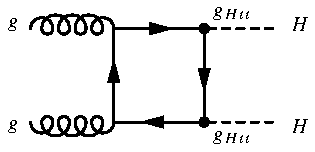
\includegraphics[width=0.7\textwidth]{feynman_graphs/di_higgs_box}
    \subcaption{}
  \end{subfigure}\hfill%
  \begin{subfigure}{0.49\textwidth}
    \centering
    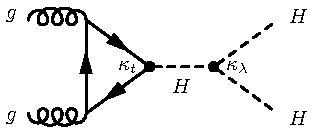
\includegraphics[width=0.7\textwidth]{feynman_graphs/di_higgs_triangle}
    \subcaption{}
  \end{subfigure}

  \vspace*{1em}

  \begin{subfigure}{0.33\textwidth}
    \centering
    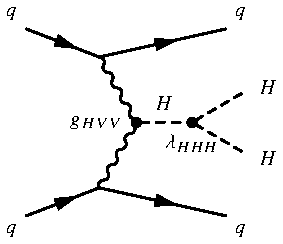
\includegraphics[width=0.95\textwidth]{feynman_graphs/di_higgs_vbf_kvklam}
    \subcaption{}
  \end{subfigure}\hfill%
  \begin{subfigure}{0.33\textwidth}
    \centering
    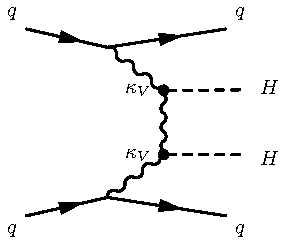
\includegraphics[width=0.95\textwidth]{feynman_graphs/di_higgs_vbf_kvkv}
    \subcaption{}
  \end{subfigure}\hfill%
  \begin{subfigure}{0.33\textwidth}
    \centering
    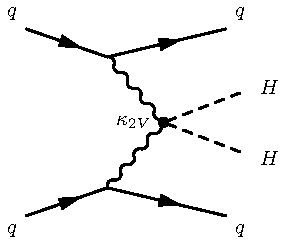
\includegraphics[width=0.95\textwidth]{feynman_graphs/di_higgs_vbf_ktwov}
    \subcaption{}
  \end{subfigure}

  \caption{Feynman graphs}
  \label{fig:hh_feynmans}
\end{figure}

\begin{figure}[htbp]
  \centering
  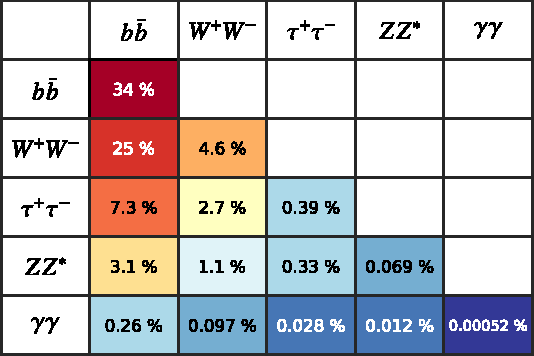
\includegraphics[width=0.45\textwidth]{theory/di_higgs_branching_ratio}
  \caption{Possible final states of decays of pairs of Standard Model
    Higgs bosons. Higgs boson branching ratios are taken
    from~\cite{deFlorian:2016spz} and
    assume~$m_{\PH} = \SI{125.0}{\GeV}$. The decay
    mode~$\PH \ra \Pgluon\Pgluon$ is excluded due to limited
    experimental feasibility.}
  \label{fig:hh_branching_ratios}
\end{figure}

4b: Very large branching ratio but huge multi-jet background.

bbtautau: Can suppress multi-jet background reasonably but large
backgrounds from EW and top.

bbyy: Very clean, but low BR.

Sensitivity vs mass:

bbyy: Low mass sensitivity (due to low threshold photon triggers)

bbtautau: Medium mass sensitivity

bbbb: High mass sensitivity (BR and reduced problems in finding Higgs
candidates due to boost)

\todo[inline]{Experimental evidence for the top Yukawa coupling exists
  therefore non-resonant \HH production has to exist too (at least via
  the box diagram)}

\begin{description}


\item[Vacuum Stability] The present minimum with a vacuum expectation
  value of $v \approx \si{246}{\GeV}$ might be either a global minimum
  in which case the universe is stable or only a local minimum which
  leads to a metastable universe. In the metastable case, the state of
  the Higgs field could tunnel to a new local or global minimum with a
  smaller vacuum expectation value. Current experimental data cannot
  distinguish whether the universe is stable or
  meta-stable\todo{citation}.

\item[Elektroweak phase transition] In baryogenesis a first order
  electroweak phase transition is needed.

\item[BSM] Radions, 2HDM, Warped extra dimensions, composite Higgs,
  hMSSM, KK Gravitons: Most could decay to pairs of SM Higgs bosons.

\end{description}

Single Higgs boson production cross section
$\approx \SI{50}{\pico\barn}$. Compared to Higgs pair production cross
section $\approx \SI{30}{\femto\barn}$.

\todo[inline]{Shortcomings of the SM: Hierarchy problem, dark matter, quantum
  description of gravity}

\todo[inline]{Maybe: SUSY - superpartners - cancellation of loop corrections to $h$
  mass; In R-parity conserving SUSY - LSP - DM candidate}

\todo[inline]{What models predict Spin-0 resonances decaying into pair of SM
  Higgs? 2HDM}

\todo[inline]{Mention Spin-2 resonances? KK-graviton -- theoretically not favoured}

\todo[inline]{Scalar sector relatively unexplored?}

%%% Local Variables:
%%% mode: latex
%%% TeX-master: "../../phd_thesis"
%%% End:

\section{Physics Beyond the Standard Model}%
\label{sec:bsm}

The SM is among the most precisely tested theories of physics. It had numerous
successes in predicting phenomena before they were experimentally observed. For
example, the SM predicted the existence of gluons, the $W^\pm$ and $Z$ bosons,
and the Higgs boson prior to their discovery.
% Most recently, the Higgs boson was discovered in 2012 about five decades after
% the inclusion of the BEH mechanism into the SM by Weinberg in
% 1967~\cite{Weinberg:1967tq}. Similarly, the gluons, $W^\pm$ and $Z$ bosons
% were all predicted by the SM before direct experimental evidence for their
% existence could be obtained.
Despite its many successes, the SM is known to be an incomplete theory leaving a
number of phenomena unexplained:
\begin{description}

\item[Matter-antimatter asymmetry] In current cosmological models, equal amounts
  of matter and antimatter are produced in the initial phase of the evolution of
  the universe. However, the universe observed today mostly consists of matter
  particles. This fact is referred to as the matter-antimatter asymmetry of the
  universe. According to the conditions proposed by
  Sakharov~\cite{Sakharov:1967dj}, violation of CP symmetry is required for the
  generation of such an asymmetry in the early universe. While CP violation has
  been observed in the quark sector~\cite{Christenson:1964fg} and first
  indications of CP violation in the lepton sector exist~\cite{T2K:2019bcf}, its
  size might not be sufficient to explain the observed asymmetry.

\item[Gravitation] The theory of general relativity provides an accurate
  description of gravitation in the context of a classical field
  theory. However, no generally accepted approach exists that reconciles general
  relativity with the quantum theory underlying our current formulation of the
  SM. Moreover, understanding the weakness of gravitational interactions at the
  scale of elementary particles remains one of the open questions in particle
  physics.

\item[Dark matter] Astrophysical
  observations~\cite{Zwicky:1933gu,Zwicky:1937zza,Rubin:1970zza,Rubin:1980zd,Clowe:2006eq}
  indicate that the vast majority of the universe consists of a form of matter,
  referred to as \emph{dark matter}, that does not interact via the
  electromagnetic interaction. However, its existence can be inferred from the
  gravitational interaction between dark and ordinary matter. Provided dark
  matter is microscopic in nature, the SM does not provide a suitable dark
  matter candidate that is consistent with current cosmological models.

\item[The electroweak hierarchy problem] The mass of the Higgs boson is affected
  by virtual corrections involving loops of massive particles. These corrections
  diverge quadratically with the momentum scale $\Lambda$~\cite{Giudice:2008bi},
  which is the upper cut-off of the loop momentum integration. Based on
  arguments of
  \emph{naturalness}~\cite{Gildener:1976ai,Weinberg:1978ym,Susskind:1978ms,Giudice:2008bi},
  the radiative corrections to the Higgs boson mass should not exceed the
  electroweak scale of $\mathcal{O}(\SI{100}{\GeV})$. Under this assumption, the
  SM cannot remain valid beyond a scale of $\mathcal{O}(\SI{1}{\TeV})$, at which
  point the divergences would have to be regulated by BSM physics
  contributions. At the LHC, the SM is being probed at this scale and beyond,
  however, no direct signs of new physics have been observed thus
  far. Consequently, it needs to be considered that the SM remains valid up to a
  larger energy scale, for example the scale of a \emph{Grand Unified Theory}
  (GUT) of about $10^{16}\,\si{\GeV}$~\cite{pdg2020}. In this case, for the
  Higgs boson mass to remain at the electroweak scale would require excessive
  \emph{fine-tuning} of the theory parameters, otherwise radiative corrections
  would drag the Higgs boson mass towards, for example, the GUT scale.

\item[Neutrino masses] The observation of neutrino
  oscillations~\cite{Super-Kamiokande:1998kpq,SNO:2002tuh} constitutes
  experimental evidence of neutrinos being massive particles. In the SM, it is
  assumed that neutrinos are massless particles, however. Extending the SM to
  incorporate non-vanishing neutrino masses poses the question whether neutrinos
  are Dirac or Majorana~\cite{Majorana:1937vz} particles. In addition, upper
  limits on the neutrino masses are $\mathcal{O}(\SI{1}{\electronvolt})$ for
  electron-based measurements~\cite{KATRIN:2019yun}, which
  % , adopting arguments of \emph{naturalness},
  appear to be unnaturally small compared to the mass scales of other fermions
  (\SI{1}{\MeV} to \SI{100}{\GeV}).

  % If neutrinos are Dirac particles, then a
  % Dirac mass term can be introduced into the SM Lagrangian via Yukawa
  % interactions between neutrinos and the Higgs boson. This mass term couples
  % left- and right-handed neutrino chiral states, implying the existence of a
  % non-interacting (\emph{sterile}) degree of freedom.

  % If neutrinos are Dirac particles, then the
  % addition of a Dirac mass term into the SM Lagrangian introduces a coupling
  % between left- and right-handed neutrino chiral states. This implies the
  % existence of a non-interacting (\emph{sterile}) degree of freedom for
  % neutrinos, since right-handed neutrinos (left-handed anti-neutrinos) do not
  % participate in the weak interaction. While the neutrino masses could be
  % generated via Yukawa couplings to the Higgs field, the coupling strengths
  % differ by many orders of magnitude compared to other fermions. The alternative
  % hypothesis of neutrinos being Majorana particles~\cite{Majorana:1937vz}, i.e.\
  % neutrinos are their own anti-particles,

  % - lepton number violation (neutrinoless double-$\beta$ decay)

  % \emph{see-saw mechanism}

  % Majorana:
  % - Neutrinos and antineutrinos are the same particle
  % - No sterile neutrinos
  % - Seesaw mechanism could explain the small mass of neutrinos

% Is this really a 'problem'?
% \item[Vacuum Stability] The present minimum with a vacuum expectation value of
%   $\varv \approx \si{246}{\GeV}$ might be either a global minimum in which case the
%   universe is stable or only a local minimum which leads to a metastable
%   universe. In the metastable case, the state of the Higgs field could tunnel to
%   a new local or global minimum with a smaller potential. Current experimental
%   data cannot distinguish whether the universe is stable or
%   meta-stable\todo{citation}.

\end{description}
Even though the SM has its shortcomings, it describes many natural phenomena
with excellent precision. Thus, it is often believed that the SM represents the
low-energy manifestation of an extended theory that only becomes relevant at
larger energy scales, for example a \emph{Grand Unified Theory} that unifies the
electroweak and strong interaction.


\subsection{Non-Resonant Higgs Boson Pair Production}%
\label{sec:bsm_nonresonant_hh}

BSM phenomena might appear at energy scales beyond what can be experimentally
probed using direct searches at the LHC. Nevertheless, it is possible to test
such models indirectly through their effect on SM processes via virtual
corrections. These corrections can, for example, alter the total or differential
cross section of a given process.
% Therefore, searches for non-resonant \HH production are already of interest,
% since an enhancement in its cross section would be indicative of BSM physics.

% Another way...
A way of exploring BSM contributions to non-resonant \HH production is to
examine the Higgs boson self-coupling constant for possible deviations from the
SM value of $\lambda_{HHH}^\text{SM} = 3 m_{H}^2 / \varv$. Such deviations can
similarly arise due to virtual corrections involving massive BSM particles as
indicated in \Cref{fig:bsm_hh_prod_feyn}. If the mass scale of the particles
participating in the corrections is sufficiently large, then the dynamics of the
BSM theory can be reduced to an effective interaction vertex between three Higgs
bosons with a coupling constant
\begin{align*}
  \lambda_{HHH} = \klambda \times \lambda_{HHH}^{\text{SM}} \,\text{,}
\end{align*}
where \klambda is an arbitrary coupling modifier. Due to the interference with
the $\pp \to HH$ box diagram previously depicted in
\Cref{fig:dihiggs_ggf_feyn_box}, a change in \klambda will alter both the total
cross section of non-resonant \HH production and the kinematics of the final
state particles. A detailed discussion of these effects will follow in
\Cref{sec:higgs_self_coupling}.

\begin{figure}[htbp]
  \centering

  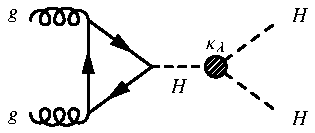
\includegraphics[width=0.35\textwidth]{feynman_graphs/di_higgs_effective}

  \caption[Feynman diagram of non-resonant \HH production with anomalous values
  of the Higgs boson self-coupling.]{Non-resonant production of Higgs boson
    pairs for anomalous values of the Higgs boson self-coupling constant.
    Contributions of new physics, for example through loops of heavy BSM
    particles, are indicated as a hatched circle. The effective coupling
    constant in units of the self-coupling constant predicted by the SM is given
    by \klambda.}%
  \label{fig:bsm_hh_prod_feyn}
\end{figure}

% Unitarity: Scattering probability < 1
%
% Perturbativity: Higher-order corrections become smaller as opposed to larger
Current bounds on possible values of \klambda from requirements of perturbative
unitarity in $HH \to HH$ scattering allow for variations within
$|\klambda| \lessapprox 6$~\cite{DiLuzio:2017tfn}.\footnote{Similar arguments
  were made in the past to obtain upper limits on the Higgs boson mass from
  unitarity bounds in the scattering of longitudinally polarised vector
  bosons~\cite{Lee:1977eg}.} These bounds still allow for ample variation of the
Higgs boson self-coupling strength, further motivating searches for non-resonant
\HH production. These searches constitute a major part of
\Cref{sec:dihiggs,sec:higgs_self_coupling}, in which upper limits are set on the
non-resonant \HH production cross section of a signal with SM-like
($\klambda = 1$) kinematics, and signals with anomalous \klambda
($\klambda \neq 1$), respectively.

% Anomalous values of the Higgs boson self-coupling within
% $|\klambda| \lessapprox 6$ are allowed given arguments based on the unitarity
% and perturbativity of $HH \to HH$
% scattering~\cite{DiLuzio:2017tfn}.\footnote{Similar arguments were made in the
%   past to obtain upper limits on the Higgs boson mass from unitarity bounds in
%   the scattering of longitudinally polarised vector bosons~\cite{Lee:1977eg}.}


\subsection{Resonant Higgs Boson Pair Production}%
\label{sec:bsm_resonant_hh}

If BSM physics occurs at experimentally accessible energy scales, new particles
could be produced directly (on-shell) in collider experiments. Further assuming
that these particles are short-lived and decay into detectable SM particles, one
can reconstruct the mass of such particles using the four-momenta of their decay
products. The presence of BSM physics can then appear as an enhancement of the
differential cross section $\mathrm{d}\sigma / \mathrm{d}m$, $m$ referring to
the invariant mass of the final state particles, in a region close to the mass
of the new particle. This phenomenon is referred to as a \emph{resonance} and
the production of particles via an intermediate resonance as \emph{resonant
  production}.

The Higgs sector is often used as an entry point for physics beyond the
SM. Aside from aesthetic reasons, there are currently no arguments that require
nature to realise a \emph{minimal Higgs model} with a single
Higgs-doublet~\cite{Gunion:1989we}. In fact, the Higgs sector can be readily
extended with additional scalar fields with singlet and doublet representations
under the SM gauge group~\cite{Gunion:1989we}. Such extended Higgs sectors are
part of many BSM theories, resulting in a phenomenology with new scalar
particles. Under certain circumstances, these models allow for a sizeable
production of SM-like Higgs boson pairs via intermediate scalar resonances. A
possible Feynman diagram of resonant Higgs boson pair production is depicted in
\Cref{fig:resonant_production_feyn}. Two examples of models with extended Higgs
sectors are given in the following.

\begin{figure}[htbp]
  \centering

  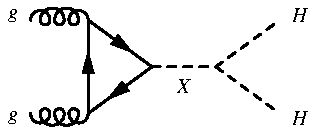
\includegraphics[width=0.35\textwidth]{feynman_graphs/di_higgs_resonant}

  \caption[Feynman diagram of resonant Higgs boson pair production.]{Resonant
    production of SM Higgs boson pairs via an intermediate scalar resonance $X$
    produced in \ggF.}%
  \label{fig:resonant_production_feyn}
\end{figure}

\begin{description}

\item[Additional Higgs-singlet models] The simplest extension of the SM Higgs
  sector is the addition of a real scalar field $\phi_{S}$ that transforms as a
  singlet under the SM gauge group. This scalar field, being a gauge singlet,
  does not interact with any of the SM fermions or vector bosons. It could
  therefore be part of a ``hidden sector'' which might provide a suitable
  candidate for dark matter. In so-called \emph{Higgs portal
    models}~\cite{Patt:2006fw}, the hidden sector can only be accessed through
  coupling/mixing of $\phi_{S}$ with the CP-even component of the SM Higgs
  field. Such models can predict resonant production of Higgs boson pairs
  through new scalar
  resonances~\cite{Schabinger:2005ei,Bowen:2007ia,Barger:2007im,Dolan:2012ac,No:2013wsa,Chen:2014ask,Robens:2016xkb,DiMicco:2019ngk}.

  A general choice for the potential of a Higgs sector extended by an additional
  scalar field
  reads~\cite{OConnell:2006rsp,No:2013wsa,Chen:2014ask,DiMicco:2019ngk}
  \begin{align*}
    V(\phi, \phi_{S}) = V(\phi)
    + \frac{a_1}{2} (\phi^\dagger \phi) \phi_{S}
    + \frac{a_2}{2} (\phi^\dagger \phi) \phi_{S}^2
    + b_1 \phi_{S} + \frac{b_2}{2} \phi_{S}^2 + \frac{b_3}{3} \phi_{S}^3 + \frac{b_4}{4} \phi_{S}^4 \,\text{,}
  \end{align*}
  where $\phi$ refers to the complex Higgs-doublet and $V(\phi)$ is the BEH
  potential. In unitary gauge, the fields can be expanded about the vacuum state
  as $\phi = (0, \varv + H)^{\text{T}} / \sqrt{2}$ and $\phi_{S} = \varv_{S} + S$, where
  $\varv_{S}$ is the VEV of $\phi_{S}$. After the expansion, terms bilinear in $H$
  and $S$ appear in the potential,\footnote{The bilinear terms only appear if
    either $a_1 \neq 0$, or $a_2 \neq 0$ and $\phi_{S}$ has non-vanishing
    VEV. See for example Ref.~\cite{Chen:2014ask}.} which indicate that the
  physical fields are mixtures of $H$ and $S$. The physical fields $H_1$ and
  $H_2$ with masses $m_1$ and $m_2$, respectively, can be expressed as
  \begin{align*}
    \begin{pmatrix}
      H_1 \\
      H_2
    \end{pmatrix}
    =
    \begin{pmatrix}
      \cos\theta & \sin\theta \\
      -\sin\theta & \cos\theta
    \end{pmatrix}
    \begin{pmatrix}
      H \\
      S
    \end{pmatrix} \,\text{,}
  \end{align*}
  with a mixing angle $\theta$. In the following, it is assumed that $H_1$ can
  be identified with the observed Higgs boson and $H_2$ is a new scalar with
  $m_2 > 2 m_1$.  The scalar $H_2$ can be produced via \ggF through the
  admixture of $H$ in $H_2$, however, suppressed by a factor of
  $\sin^2\theta$. Further, the interaction terms of the scalar potential allow
  for decays of $H_2$ into a pair of $H_1$. As a consequence, resonant
  production processes according to $\pp \to H_2 \to H_1 H_1$ are possible given
  the prior assumptions.

\item[Two-Higgs-doublet models (2HDM)] Generic 2HDM extend the Higgs sector of
  the SM by introducing an additional $SU(2)_{\text{L}}$ doublet of complex
  scalar fields~\cite{Gunion:1989we,Branco:2011iw}. Such extensions are
  motivated by theories such as supersymmetry~\cite{Haber:1984rc}, which require
  at least two Higgs-doublets to generate masses of up- ($I_3 = + 1/2$) and
  down-type ($I_3 = - 1/2$) fermions, or models of electroweak
  baryogenesis~\cite{Trodden:1998ym}, in which 2HDM can provide CP-violating
  processes necessary to generate a matter-antimatter asymmetry in the universe.
  % The class of 2HDM encompass theories with vastly different phenomenology.
  % For example, 2HDM with flavour-changing neutral currents (FCNC) at
  % tree-level exist, however, such models are in tension with the experimental
  % non-observation of tree-level FCNC~\cite{Gunion:1989we,Branco:2011iw}.

  Further discussion is restricted to flavour- and CP-conserving 2HDM, which,
  for example, include models describing the Higgs sector of minimal
  supersymmetric extensions of the SM (MSSM).\footnote{For CP-violating 2HDM as
    possible explanations of electroweak baryogenesis, see for example the
    \emph{complex 2HDM} (C2HDM) in Ref.~\cite{Fontes:2017zfn}.}
  % The Higgs doublets in 2HDM have non-vanishing VEV denoted $\varv_1$ and $\varv_2$,
  % respectively.  , often expressed as the ratio
  % $\tan\beta \coloneqq \varv_2 / \varv_1$.
  The particle spectrum of these models consist of five scalar particles after
  EWSB: two CP-even Higgs bosons $H_1$ and $H_2$, a CP-odd Higgs boson $A$, and
  two charged Higgs bosons $H^\pm$. Similar to the model with an additional
  Higgs-singlet, the physical fields $H_1$ and $H_2$ are mixed states of the
  CP-even components of both Higgs-doublets, and interaction vertices of the
  form $H_1 H_1 H_2$ exist~\cite{Gunion:1989we,Branco:2011iw}. This can allow
  for resonant production processes according to $\pp \to H_2 \to H_1 H_1$,
  which are promising search channel for heavy, CP-even Higgs boson in certain
  BSM scenarios~\cite{Dolan:2012ac,Djouadi:2013vqa,Djouadi:2013uqa}.

\end{description}
The selected examples are not intended to be comprehensive but rather serve to
illustrate how resonant \HH production can arise in models with extended Higgs
sectors. In this thesis, the benchmark signal process is the decay of a CP-even
scalar resonance, $X$, produced via \ggF into a pair of SM Higgs bosons as
depicted in \Cref{fig:resonant_production_feyn}. The width of the resonance is
assumed to be narrow such that interference with SM \HH production can be
neglected.

%%% Local Variables:
%%% mode: latex
%%% TeX-master: "../../phd_thesis"
%%% End:

\section{Previous Searches for Higgs Boson Pair Production}%
\label{seq:experimental_status}

The following summarises the experimental status of searches for Higgs boson
pair production prior to the work performed as part of this thesis. The focus
lies on results of the ATLAS and CMS collaborations obtained using \pp~collision
datasets at $\sqrt{s} = \SI{13}{\TeV}$ collected during the 2015 and 2016
data-taking periods at the LHC.


\subsection*{Searches for SM Higgs Boson Pair Production}%
\label{sec:past_results_smhh}

% https://cms-results.web.cern.ch/cms-results/public-results/publications/HIG-17-030/index.html

The ATLAS and CMS collaborations set upper limits on the cross section of SM \HH
production via \ggF, $\sigma_{\ggF}$, at \SI{95}{\percent} CL. The results of
both collaborations are summarised in \Cref{fig:prior_status_smhh}. Searches for
SM \HH production were performed in various channels, the \bbbb, \bbtautau, and
\bbyy channels being the most sensitive ones. A statistical combination of SM
\HH searches was performed by both collaborations. The observed (expected) upper
limits on $\sigma_{\ggF} / \sigma_{\ggF}^{\text{SM}}$ of the combination are
$6.9$ ($10$) and $22.2$ ($12.8$) ATLAS and CMS collaboration,
respectively~\cite{HDBS-2018-58,CMS-HIG-17-030}. These were the most stringent
limits on SM~\HH production at the time.

\begin{figure}[htbp]
  \centering

  \begin{subfigure}[b]{0.9\textwidth}
    \centering

    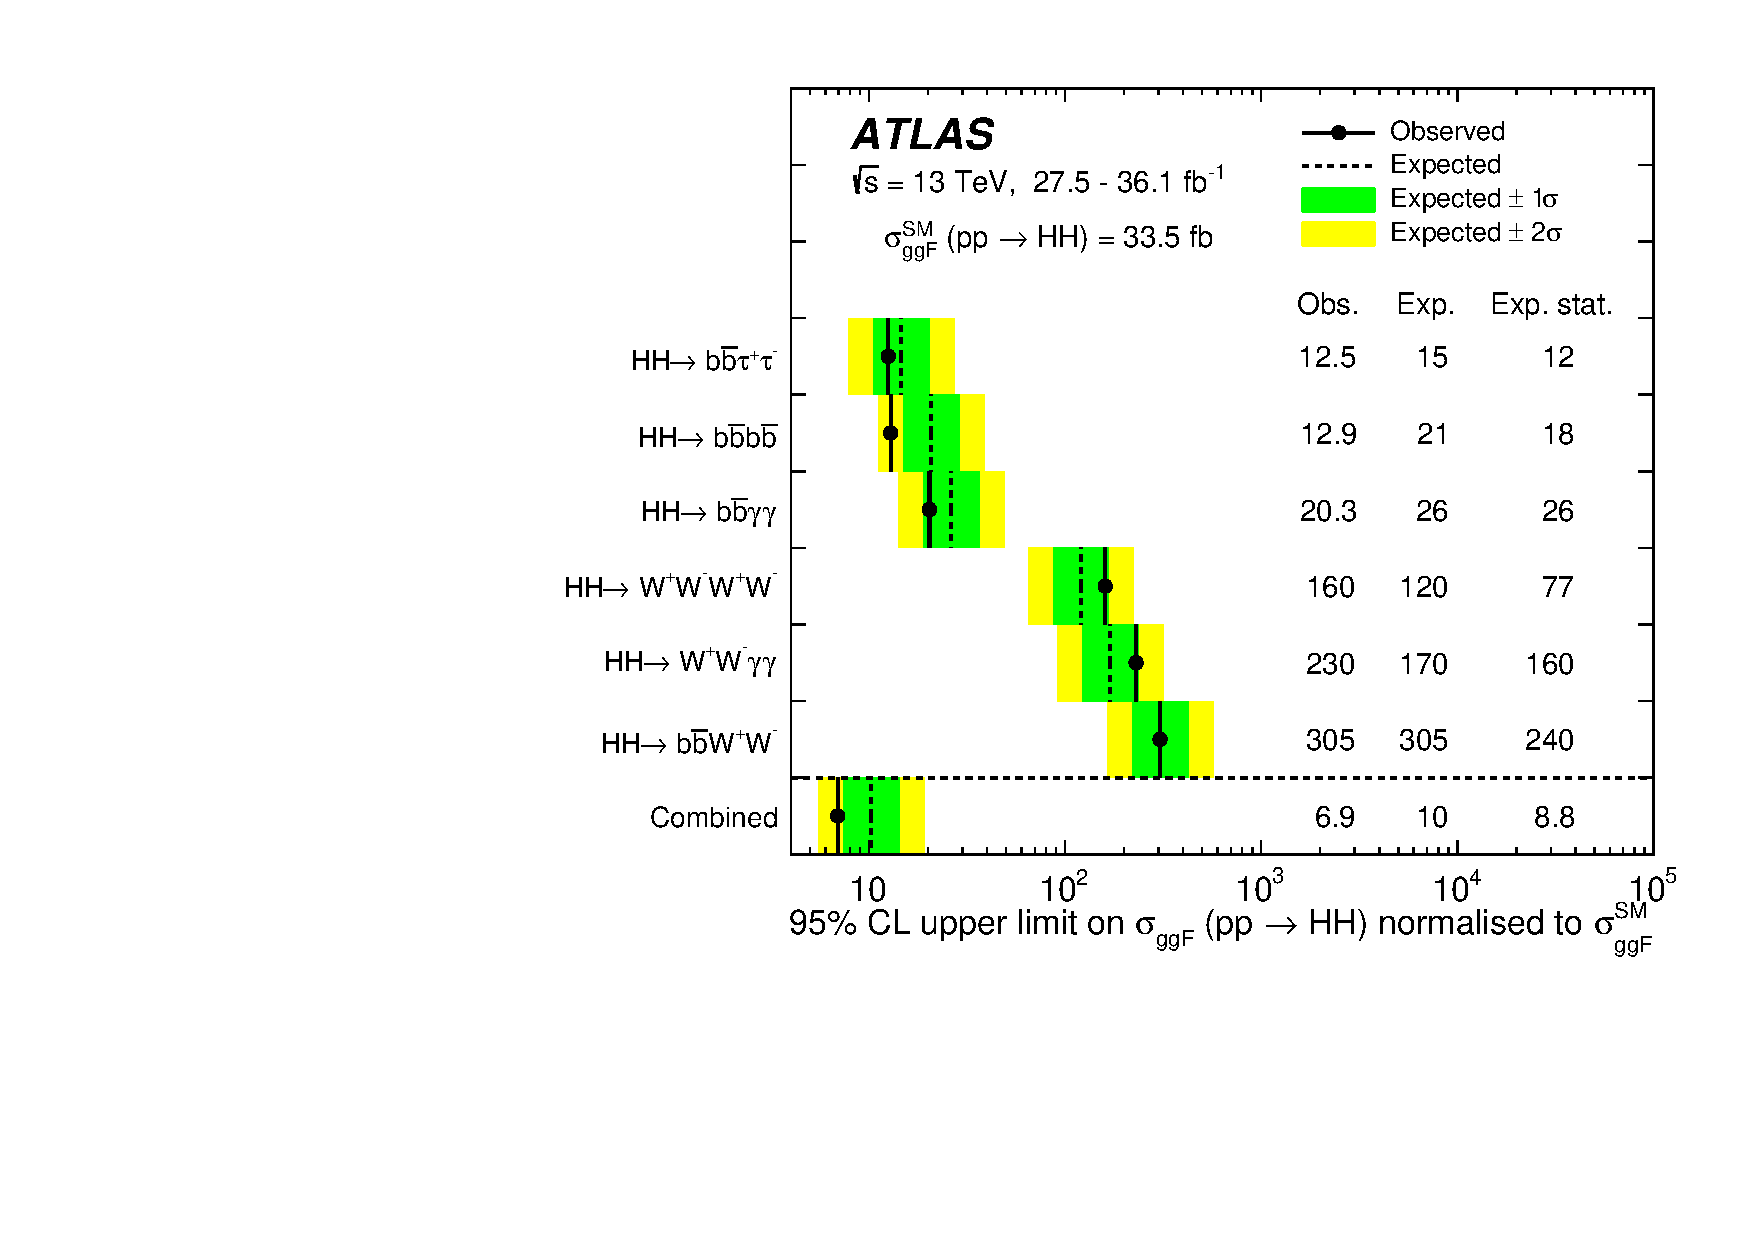
\includegraphics[width=0.62\textwidth, trim=0 0.4em 0 0,
    clip]{status/atlas_36ifb}

    \subcaption{Results of SM \HH searches by the ATLAS collaboration.  Upper
      limits excluding systematic uncertainties are given in the ``Exp.\ stat.''
      column.  The figure is taken from Ref.~\cite{HDBS-2018-58}.}
  \end{subfigure}

  \vspace{0.5em}

  \begin{subfigure}[b]{0.9\textwidth}
    \centering

    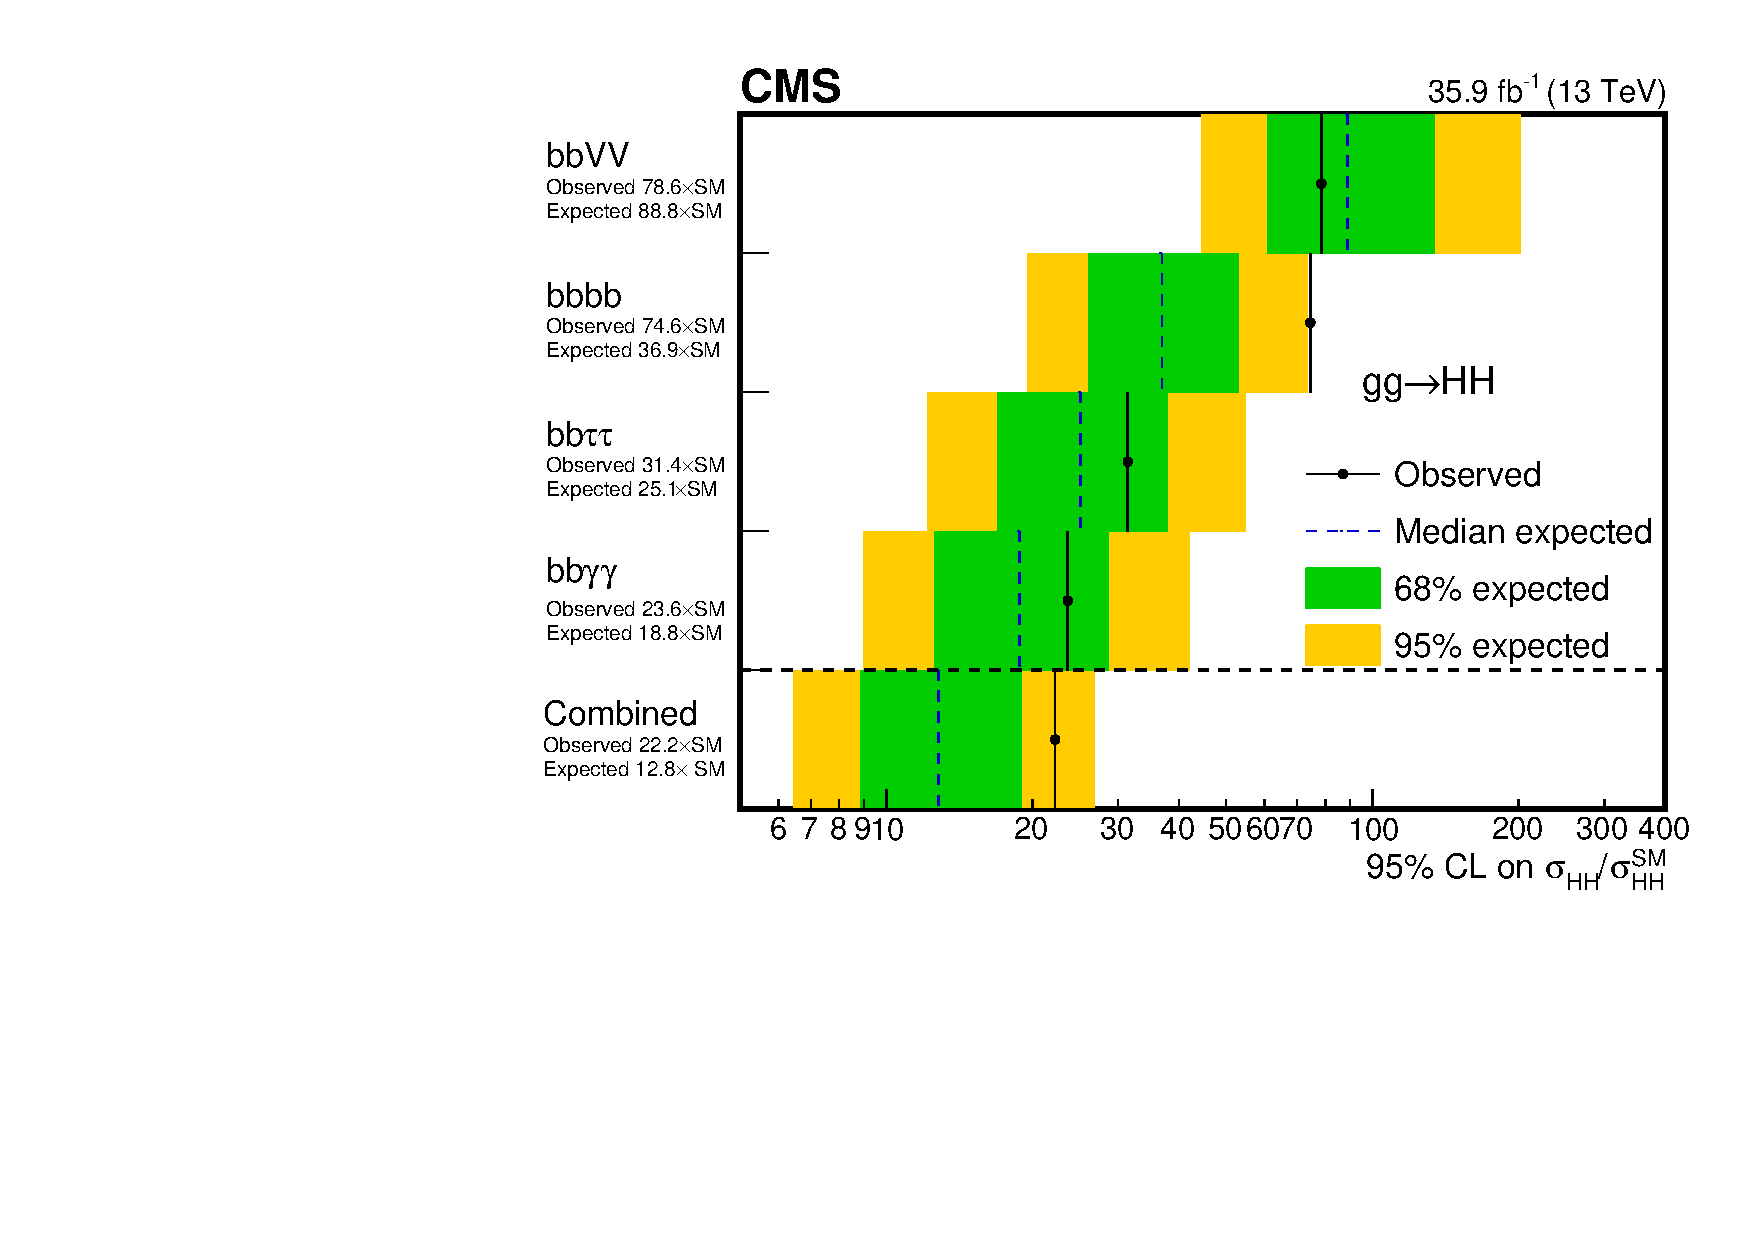
\includegraphics[width=0.62\textwidth]{status/cms_36ifb}

    \subcaption{Results of SM \HH searches by the CMS collaboration. The
      $\bbbar V V$ ($V = Z$ or $W^\pm$) channel targets final states with two
      charged leptons. The figure is taken from Ref.~\cite{CMS-HIG-17-030}.}
  \end{subfigure}

  \caption[Upper limits on the SM~\HH production cross section by the ATLAS and
  CMS collaborations at the beginning of Run~2 of the LHC.]{Upper limits at
    \SI{95}{\percent} CL on the cross section of SM \HH production via \ggF by
    the ATLAS (a) and CMS (b) collaborations. The upper limits are normalised to
    a SM cross section prediction of $\sigma_{\ggF} = \SI{33.5}{\femto\barn}$
    and given separately for the individual channels, and the statistical
    combination of all listed channels. In both cases, the expected limits are
    derived under the background-only hypothesis (i.e.\ no SM \HH
    production). The results are based on \pp~collision data taken at the
    beginning of Run~2 of the LHC.}%
  \label{fig:prior_status_smhh}
\end{figure}


\subsection*{Constraints on the Strength of the Higgs Boson Self-Coupling}%
\label{sec:past_results_klambda}

The ATLAS and CMS collaborations reinterpreted the searches for SM \HH
production in the context of anomalous values of the trilinear Higgs boson
self-coupling constant. Upper limits at \SI{95}{\percent} CL were set on the
cross section of non-resonant \HH production as a function of the Higgs boson
self-coupling modifier, \klambda. All other couplings were fixed to their SM
values. The results of both collaborations are summarised in
\Cref{fig:prior_status_klambda}. The \klambda interval in which the upper limit
on the cross section does not exclude cross section predicted by theory is
considered as the \emph{allowed \klambda interval}. The results depicted in
\Cref{fig:prior_status_klambda} yield allowed \klambda intervals of
\begin{align*}
  -5.0 < \klambda < 12.0 \,\text{(observed)} \qquad -5.8 < \klambda < 12.0 \,\text{(expected)}
\end{align*}
for the result of the ATLAS collaboration~\cite{HDBS-2018-58} and
\begin{align*}
  -11.8 < \klambda < 18.8 \,\text{(observed)} \qquad -7.1 < \klambda < 13.6 \,\text{(expected)}
\end{align*}
for the result of the CMS collaboration~\cite{CMS-HIG-17-030}.

\begin{figure}[htbp]
  \centering

  \begin{subfigure}[b]{0.9\textwidth}
    \centering

    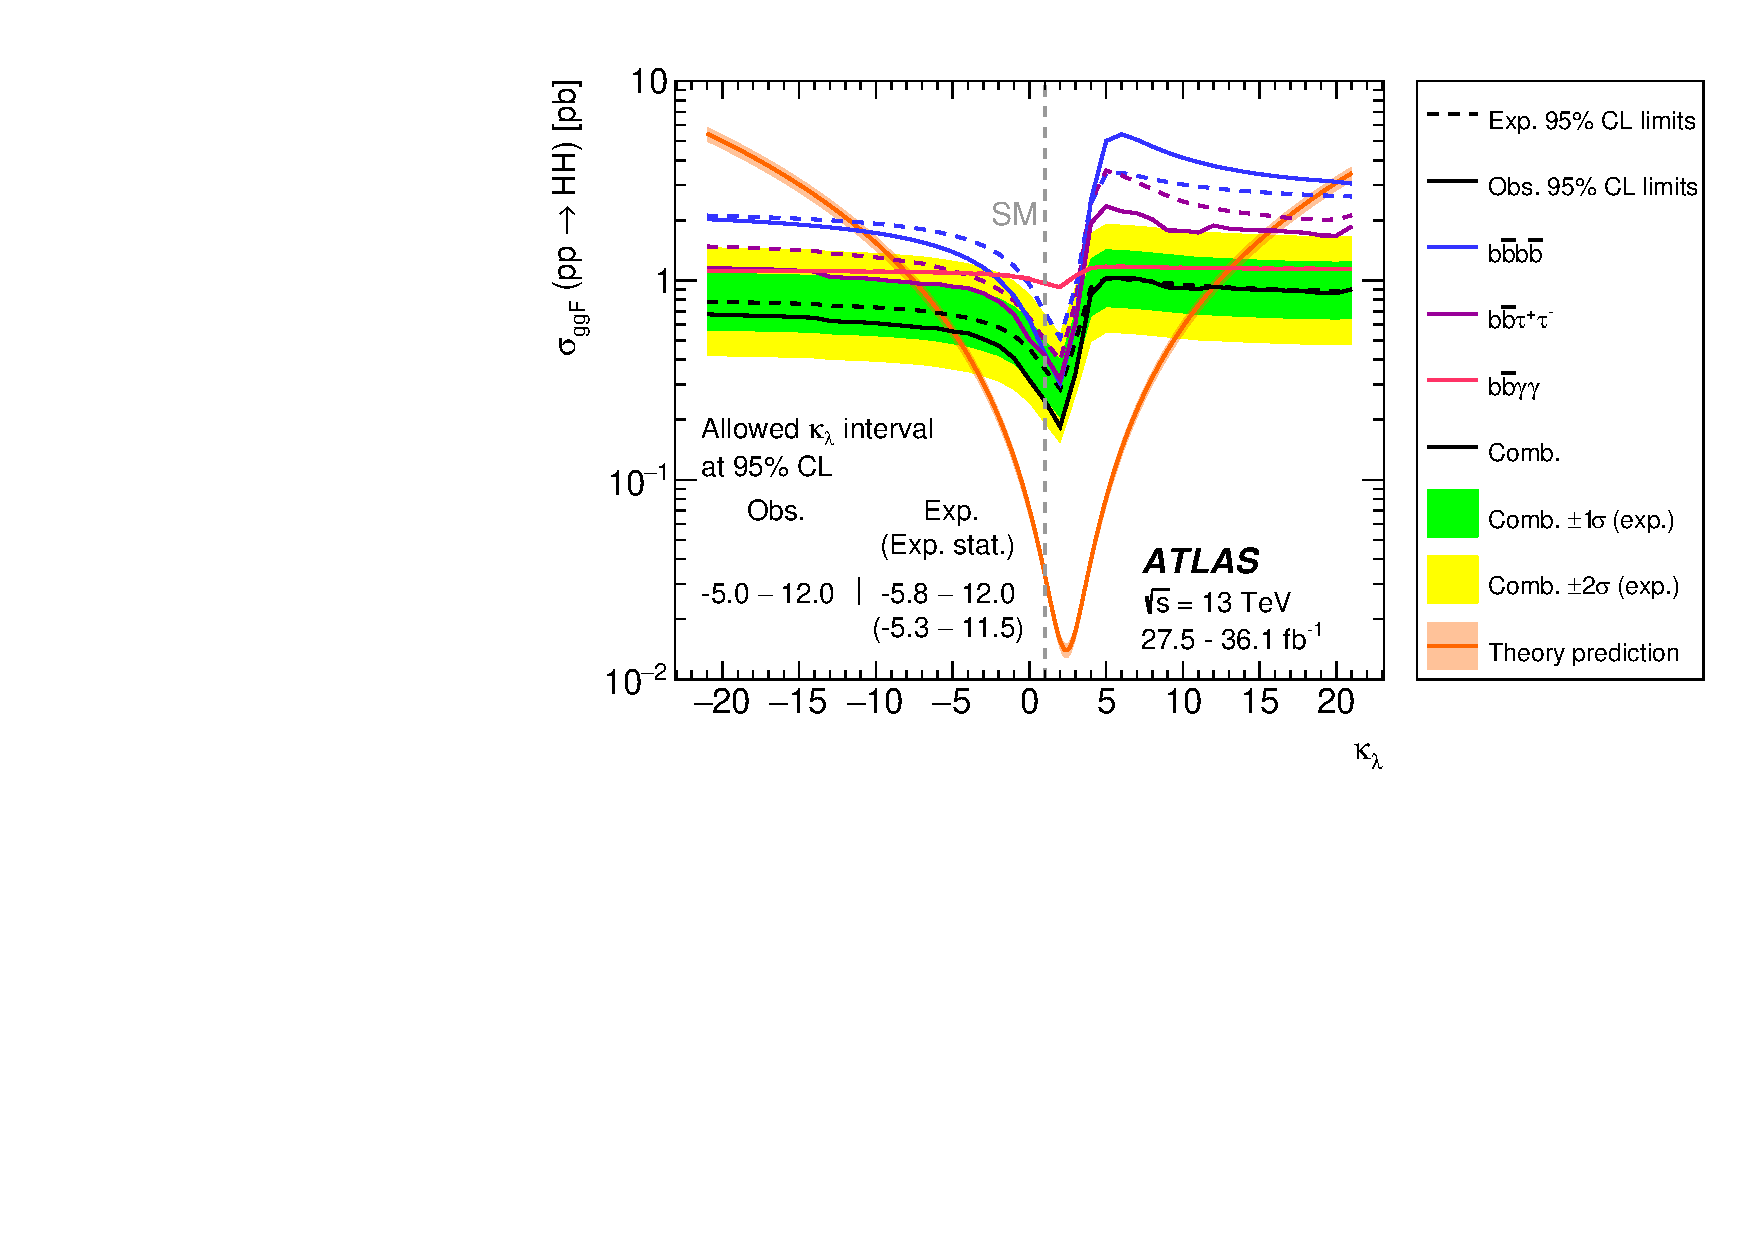
\includegraphics[width=0.67\textwidth, trim=0 1.2em 0 0,
    clip]{status/atlas_36ifb_klambda}

    % trim={<left> <lower> <right> <upper>}

    \subcaption{Results of the ATLAS collaboration for the \bbbb, \bbtautau, and
      \bbyy channels and their combination. The figure is taken from
      Ref.~\cite{HDBS-2018-58}.}
  \end{subfigure}

  \vspace{0.5em}

  \begin{subfigure}[b]{0.9\textwidth}
    \centering

    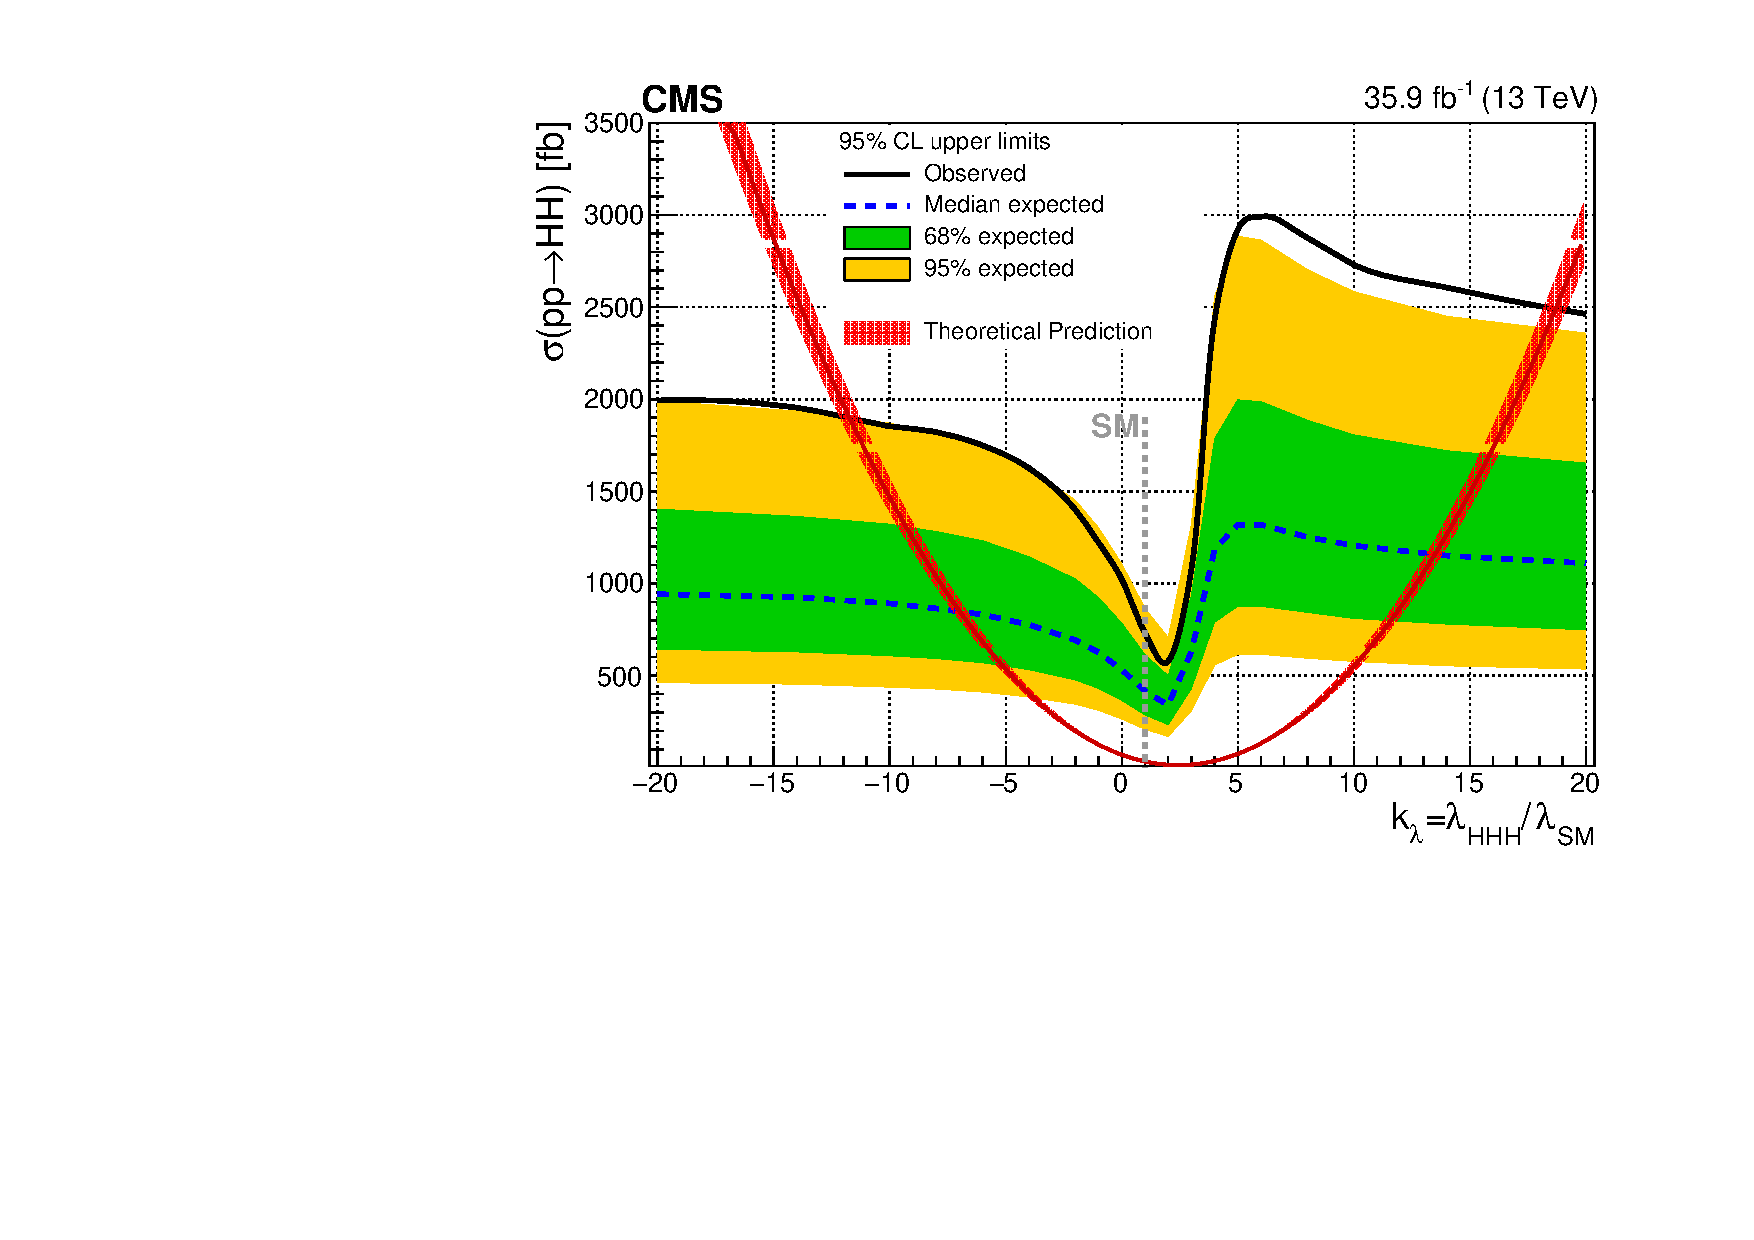
\includegraphics[width=0.58\textwidth]{status/cms_36ifb_klambda}

    \subcaption{Results of the CMS collaboration for the combination of the
      \bbbb, \bbtautau, \bbyy, and $\bbbar VV$ channels. The figure is taken
      from Ref.~\cite{CMS-HIG-17-030}.}
  \end{subfigure}

  \caption[Upper limits on the non-resonant \HH production cross section as a
  function of \klambda by the ATLAS and CMS collaborations at the beginning of
  Run~2 of the LHC.]{Upper limits at \SI{95}{\percent} CL on the cross section
    of non-resonant \HH production as a function of \klambda by the ATLAS (a)
    and CMS (b) collaborations. The expected upper limits are obtained under the
    background-only assumption (i.e.\ no non-resonant \HH production). Values of
    \klambda where the theoretical prediction exceeds the upper limit are
    excluded by the measurements. The results are based on \pp~collision data
    taken at the beginning of Run~2 of the LHC.}%
  \label{fig:prior_status_klambda}
\end{figure}


\subsection*{Searches for Resonant Production of Higgs Boson Pairs}%
\label{sec:past_results_resonant}

The ATLAS and CMS collaborations performed searches for CP-even, scalar
resonances with narrow width decaying into a pair of SM Higgs bosons. Resonance
masses ranging from the \HH production threshold up to \SI{3000}{\GeV} are
considered by both collaborations. The upper limits at \SI{95}{\percent} CL on
the production cross section of the scalar resonance as a function of its mass
are shown in \Cref{fig:prior_status_reso}. Neither the ATLAS nor the CMS result
shows a statistically significant excess in the search for resonant \HH
production.
% The excluded cross sections range from about \SI{1000}{\femto\barn} at low
% mass to about \SI{5}{\femto\barn} at high resonance mass.

\begin{figure}[htbp]
  \centering

  \newcommand*{\mybox}[1][red]{\textcolor{#1}{\rule{1.2ex}{1.2ex}}}
  \definecolor{cbbww}{RGB}{0, 153, 0}
  \definecolor{cbbtautau}{RGB}{153, 0, 153}
  \definecolor{cbbyy}{RGB}{255, 51, 102}
  \definecolor{cbbbb}{RGB}{51, 51, 255}
  \definecolor{cwwyy}{RGB}{0, 204, 204}
  \definecolor{cwwww}{RGB}{204, 102, 51}

  \begin{subfigure}[t]{0.90\textwidth}
    \centering

    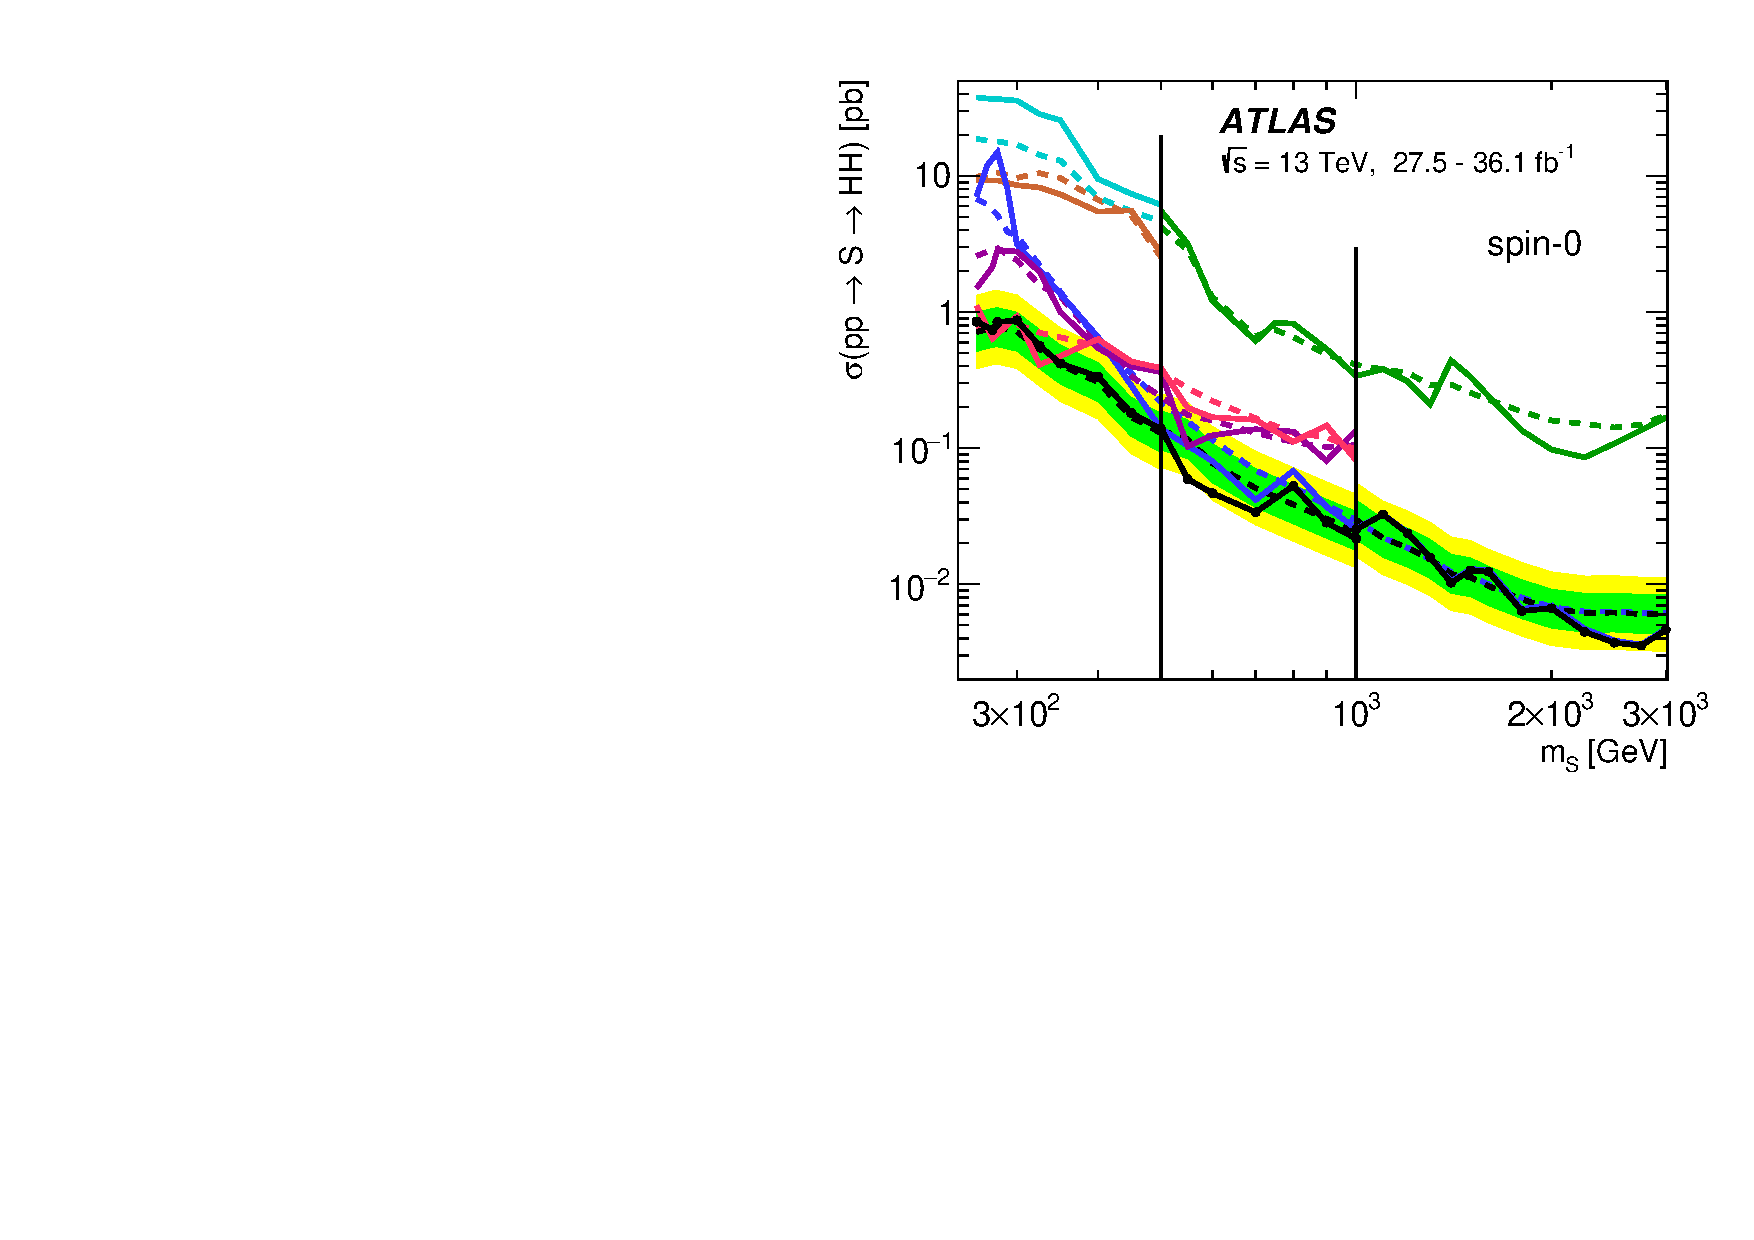
\includegraphics[width=0.52\textwidth, trim=0 0.2em 0 0,
    clip]{status/atlas_36ifb_resonant}

    \subcaption{Results of the ATLAS collaboration for the channels:
      \bbbb~(\mybox[cbbbb]), \bbtautau~(\mybox[cbbtautau]),
      \bbyy~(\mybox[cbbyy]), $\bbbar W^+ W^-$~(\mybox[cbbww]),
      $W^+ W^- \gamma\gamma$~(\mybox[cwwyy]), and
      $W^+ W^- W^+ W^-$~(\mybox[cwwww]). The statistical combination of all
      channels is shown in black. The observed (expected) upper limits are
      depicted as solid (dashed) lines. The figure is taken from
      Ref.~\cite{HDBS-2018-58}.}
  \end{subfigure}

  \vspace{0.5em}

  \begin{subfigure}[t]{0.9\textwidth}
    \centering

    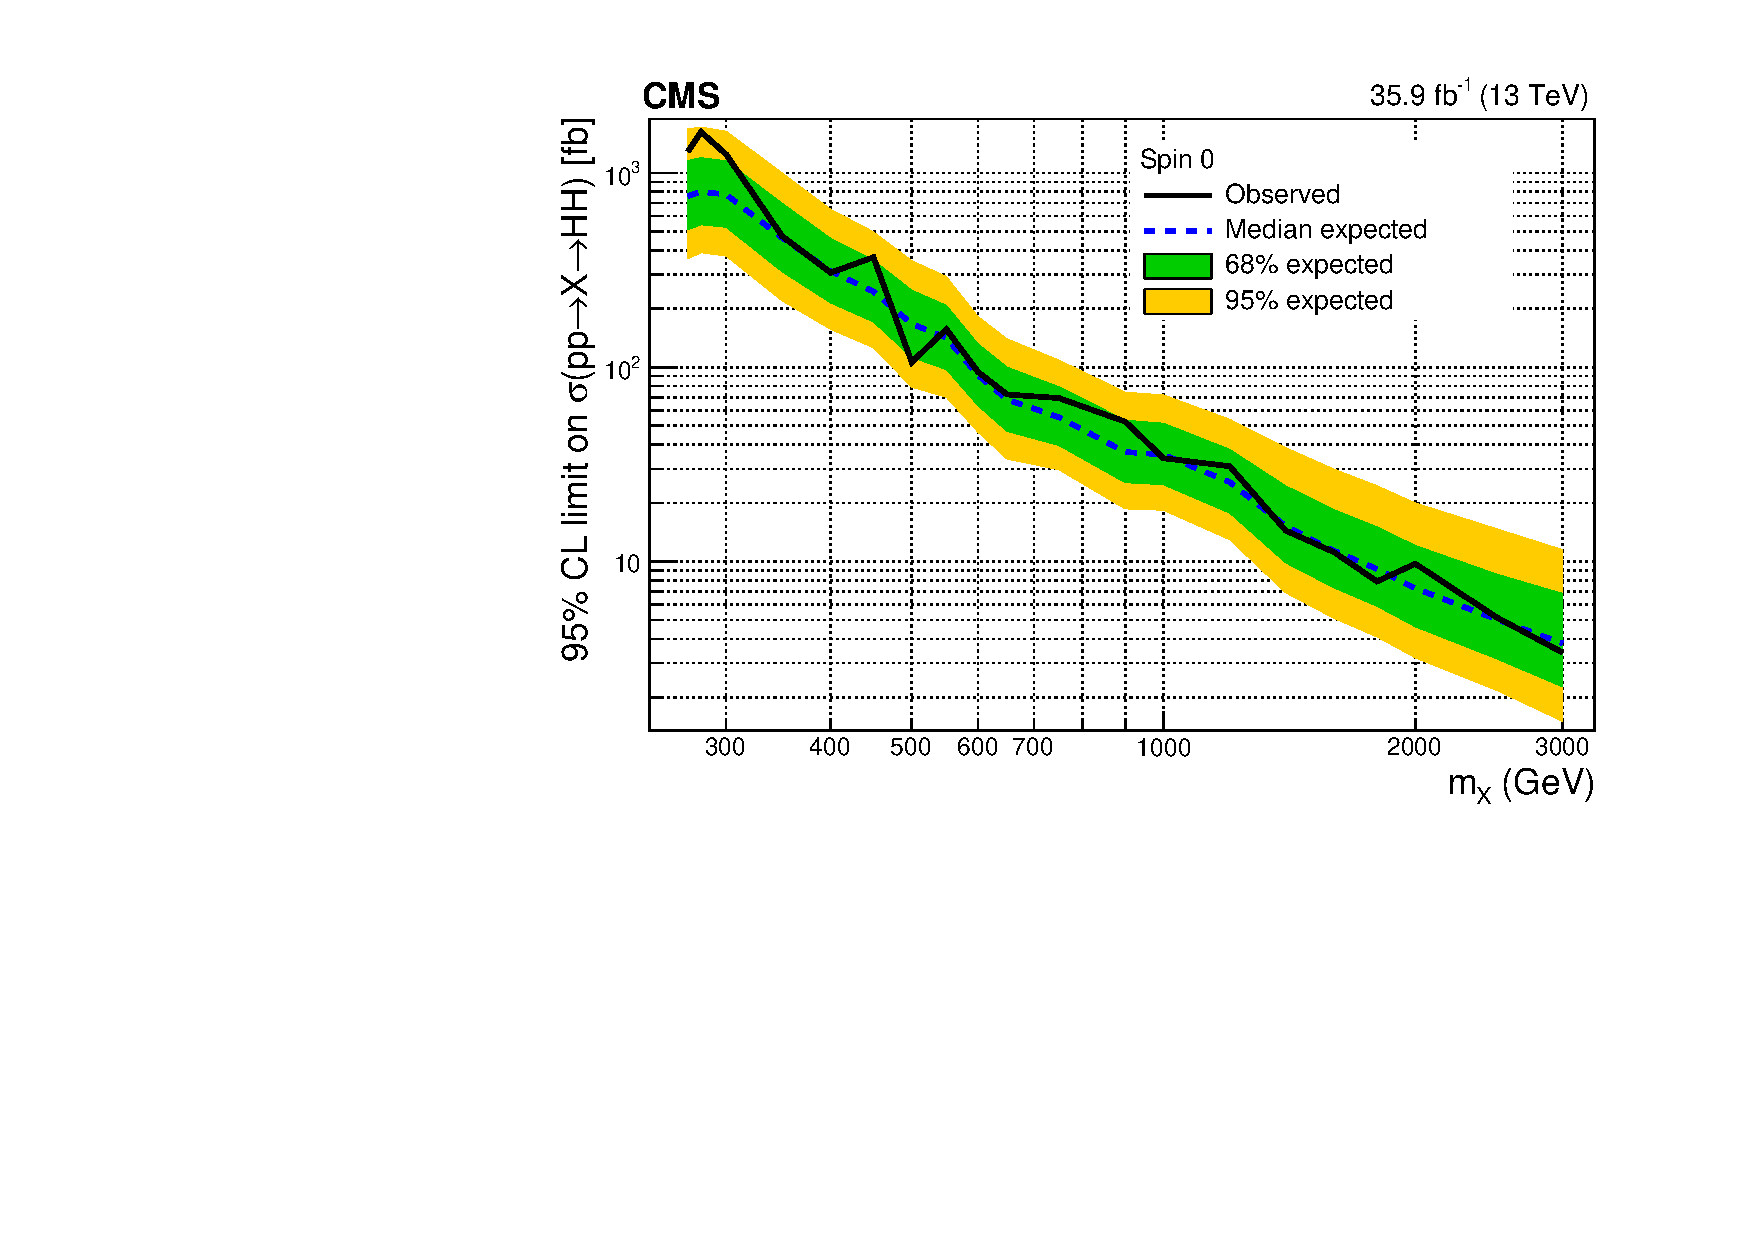
\includegraphics[width=0.6\textwidth]{status/cms_36ifb_resonant}

    \subcaption{Results of the CMS collaboration for the statistical combination
      of the \bbbb, \bbtautau, \bbyy, and $\bbbar VV$ ($V = Z$ or $W^\pm$)
      channels. The figure is taken from Ref.~\cite{CMS-HIG-17-030}.}
  \end{subfigure}

  \caption[Upper limits on the resonant \HH production cross section via scalar,
  narrow-width resonances by the ATLAS and CMS collaborations at the beginning
  of Run~2 of the LHC.]{Upper limits at \SI{95}{\percent} CL on the production
    cross section of CP-even, scalar resonances ($S$ / $X$) decaying into a pair
    of SM Higgs bosons by the ATLAS (a) and CMS (b) collaboration. The expected
    upper limits are derived assuming the background-only hypothesis. The
    results are based on \pp~collision data taken at the beginning of Run~2 of
    the LHC.}%
  \label{fig:prior_status_reso}
\end{figure}


%%% Local Variables:
%%% mode: latex
%%% TeX-master: "../../phd_thesis"
%%% End:


% \clearpage
% \todo[inline]{Here be dragons!}
% \section{Probing the Standard Model at Hadron Colliders}

Description of the hard scatter event in pp collisions:
\begin{itemize}
\item Collisions of constitutents (partons) of the protons with
  various fractions of momentum of the parent proton.

\item Factorisation approach? Factorise long-distance (soft and
  non-perturbative) and short-distance (hard and perturbative) physics
  at the factorisation scale $\mu_\text{F}$. Long-distance effects are
  factored out into the PDFs, while the partonic cross section only
  contains short-distance interactions allowing for perturbative
  expansion in \alphas. The factorisation scale separates partons
  described by the PDF (soft) and the hard scatter process. The
  calculation becomes less dependent on the scale the higher the order
  of the calculation (thus frequently used to estimate uncertainties
  on missing higher orders).

\item The partonic cross section is calculated in a perturbative
  expansion in \alphas up to some order.
\end{itemize}

\begin{align*}
  \sigma_{\Pproton\Pproton \ra \PX}() = \sum_{i,j} \int \mathrm{d}x_1 \mathrm{d}x_2 \, f_i(x_1, \muF^2) f_j(x_1, \muF^2) \, \hat{\sigma}_{i j \ra \PX}(x_1, x_2, \alphas, Q^2 / \muF^2)
\end{align*}
(Ellis, Stirling, Webber)

The inclusive cross section of proton-proton going to \PX is (factorisation approach)
\begin{align*}
  \frac{\mathrm{d}\sigma_{\Pproton\Pproton \ra \PX}}{\mathrm{d}\Omega} = \sum_{i,j} \int \mathrm{d}x_1 \mathrm{d}x_2 \int f_i(x_1) f_j(x_2) \, \mathrm{d}\hat{\sigma}_{i j \ra \PX}(x_1, x_2, \hat{s})
\end{align*}
where $i, j$ indicates the species of parton (i.e.\ gluons, quarks and
anti-quarks), $f_i(x)$ are the corresponding parton density functions,
and $\mathrm{d}\hat{\sigma}(i\,j \ra \PX)$ is the partonic cross
section at a c.m. of $\hat{s} = x_1 x_2 s$.

%%% Local Variables:
%%% mode: latex
%%% TeX-master: "../../phd_thesis"
%%% End:


% ==============================================================================
\chapter{The ATLAS Experiment at the Large Hadron Collider}%
\label{sec:atlas_and_lhc}
% ==============================================================================
This chapter describes the experimental environment surrounding the ATLAS
experiment at the Large Hadron Collider (LHC). It serves to provide a context
for the development of algorithms for the identification of hadronic decays of
\tauleptons (\Cref{sec:tauid}) and direct searches for Higgs boson pair
production (\Cref{sec:dihiggs,sec:higgs_self_coupling}) at the ATLAS
experiment. The chapter is structured as follows. The LHC is introduced in
\Cref{sec:lhc} including important parameters of the machine. In
\Cref{sec:atlas} the ATLAS detector, one of two general-purpose particle
detector experiments at the LHC, is described. The chapter concludes in
\Cref{sec:object_reco_at_atlas} by summarising the techniques used to
reconstruct particle collision events at the LHC with the ATLAS detector.

%%% Local Variables:
%%% mode: latex
%%% TeX-master: "../../phd_thesis"
%%% End:

\section{The Large Hadron Collider at CERN}%
\label{sec:lhc}

The LHC~\cite{Evans:2008zzb} is a particle collider experiment located at
CERN\footnote{From the French \emph{Conseil Européen pour la Recherche
    Nucléaire} referring to both the research organisation and the location of
  the laboratory sites.} at the French--Swiss border in Geneva, Switzerland.  At
present, the LHC is the world's highest-energy, laboratory-based particle
collider experiment accelerating protons to energies of up to \SI{6.8}{\TeV}
resulting in proton--proton (\pp) centre-of-mass energies, $\sqrt{s}$, of up to
\SI{13.6}{\TeV}. The LHC is also used to accelerate heavy-ions, however, the
focus of this section lies in the operation of the LHC in \pp-collison mode, the
analysis of \pp~collision data being the subject of this thesis.

The LHC was constructed in the former tunnel of the CERN Large Electron-Positron
Collider (LEP) with a circumference of \SI{26.7}{\kilo\metre} and became first
operational in 2008. It is a synchrotron consisting of two counter-rotating
beams of protons that are accelerated using alternating electric fields in
superconducting radio frequency resonators. The beams are bent into a cyclic
trajectory around the LHC ring using superconducting dipole magnets with field
strengths of about \SI{8}{\tesla}. Along the ring, numerous quadrupole magnets
are used for controlled focusing and defocusing of the proton beams.
% Synchrotron: 1232 dipoles (superconducting) -> Magnetic field of
% \SI{8.3}{\tesla} required for \SI{7}{\TeV} beam energy operation
The proton beams consist of localised packages of ca.\ $10^{11}$ protons,
hereafter referred to as bunches, circulating in the LHC with a minimum spacing
in time of \SI{25}{\nano\second}~\cite{Evans:2008zzb}.

The proton energies necessary for the injection into the LHC are achieved using
a sequence of particle accelerators at CERN, schematically depicted
in~\Cref{fig:cern_accelerator_complex}. Protons are first accelerated in LINAC 2
after which they pass through the Proton Synchrotron Booster (BOOSTER), the
Proton Synchrotron (PS), and the Super Proton Synchrotron (SPS). The SPS
accelerates protons to an energy of \SI{450}{\GeV}~\cite{Evans:2008zzb},
subsequently injecting the protons into the LHC. In the LHC, the protons are
further accelerated until the target energy is reached. Afterwards, the beams
are brought into collision at four points, the interaction points (IPs), along
the ring. Four large experiments are situated at the IPs to observe and record
particle collision events: ATLAS~\cite{PERF-2007-01}, CMS~\cite{CMS-CMS-00-001},
ALICE~\cite{ALICE:2008ngc}, and LHCb~\cite{LHCb:2008vvz}. The ATLAS and CMS
experiments are particle detector experiments targeting largely overlapping,
extensive physics programmes, while the ALICE and LHCb adopt more specialised
programmes. The ALICE experiment studies the production of the quark-gluon
plasma, a state of matter with asymptotically free quarks and gluons occurring
at temperatures similar to those right after the Big Bang, in heavy-ion
collisions. The LHCb experiment investigates the nature the matter-antimatter
asymmetry in the universe by studying CP violation in decays of hadrons
containing $b$-quarks. Several smaller experiments are installed at the LHC to
study physics processes at small angles with respect to the LHC beamline or
search for exotic particles. These experiments are LHCf~\cite{LHCf:2008lfy},
TOTEM~\cite{TOTEM:2008lue}, and MoEDAL~\cite{MoEDAL:2009jwa}.\footnote{For the
  data-taking period starting in 2022, two additional experiments called
  FASER~\cite{FASER:2019aik} and SND@LHC~\cite{Boyarsky:2021moj} were
  comissioned.}


\begin{figure}[htbp]
  \centering

  %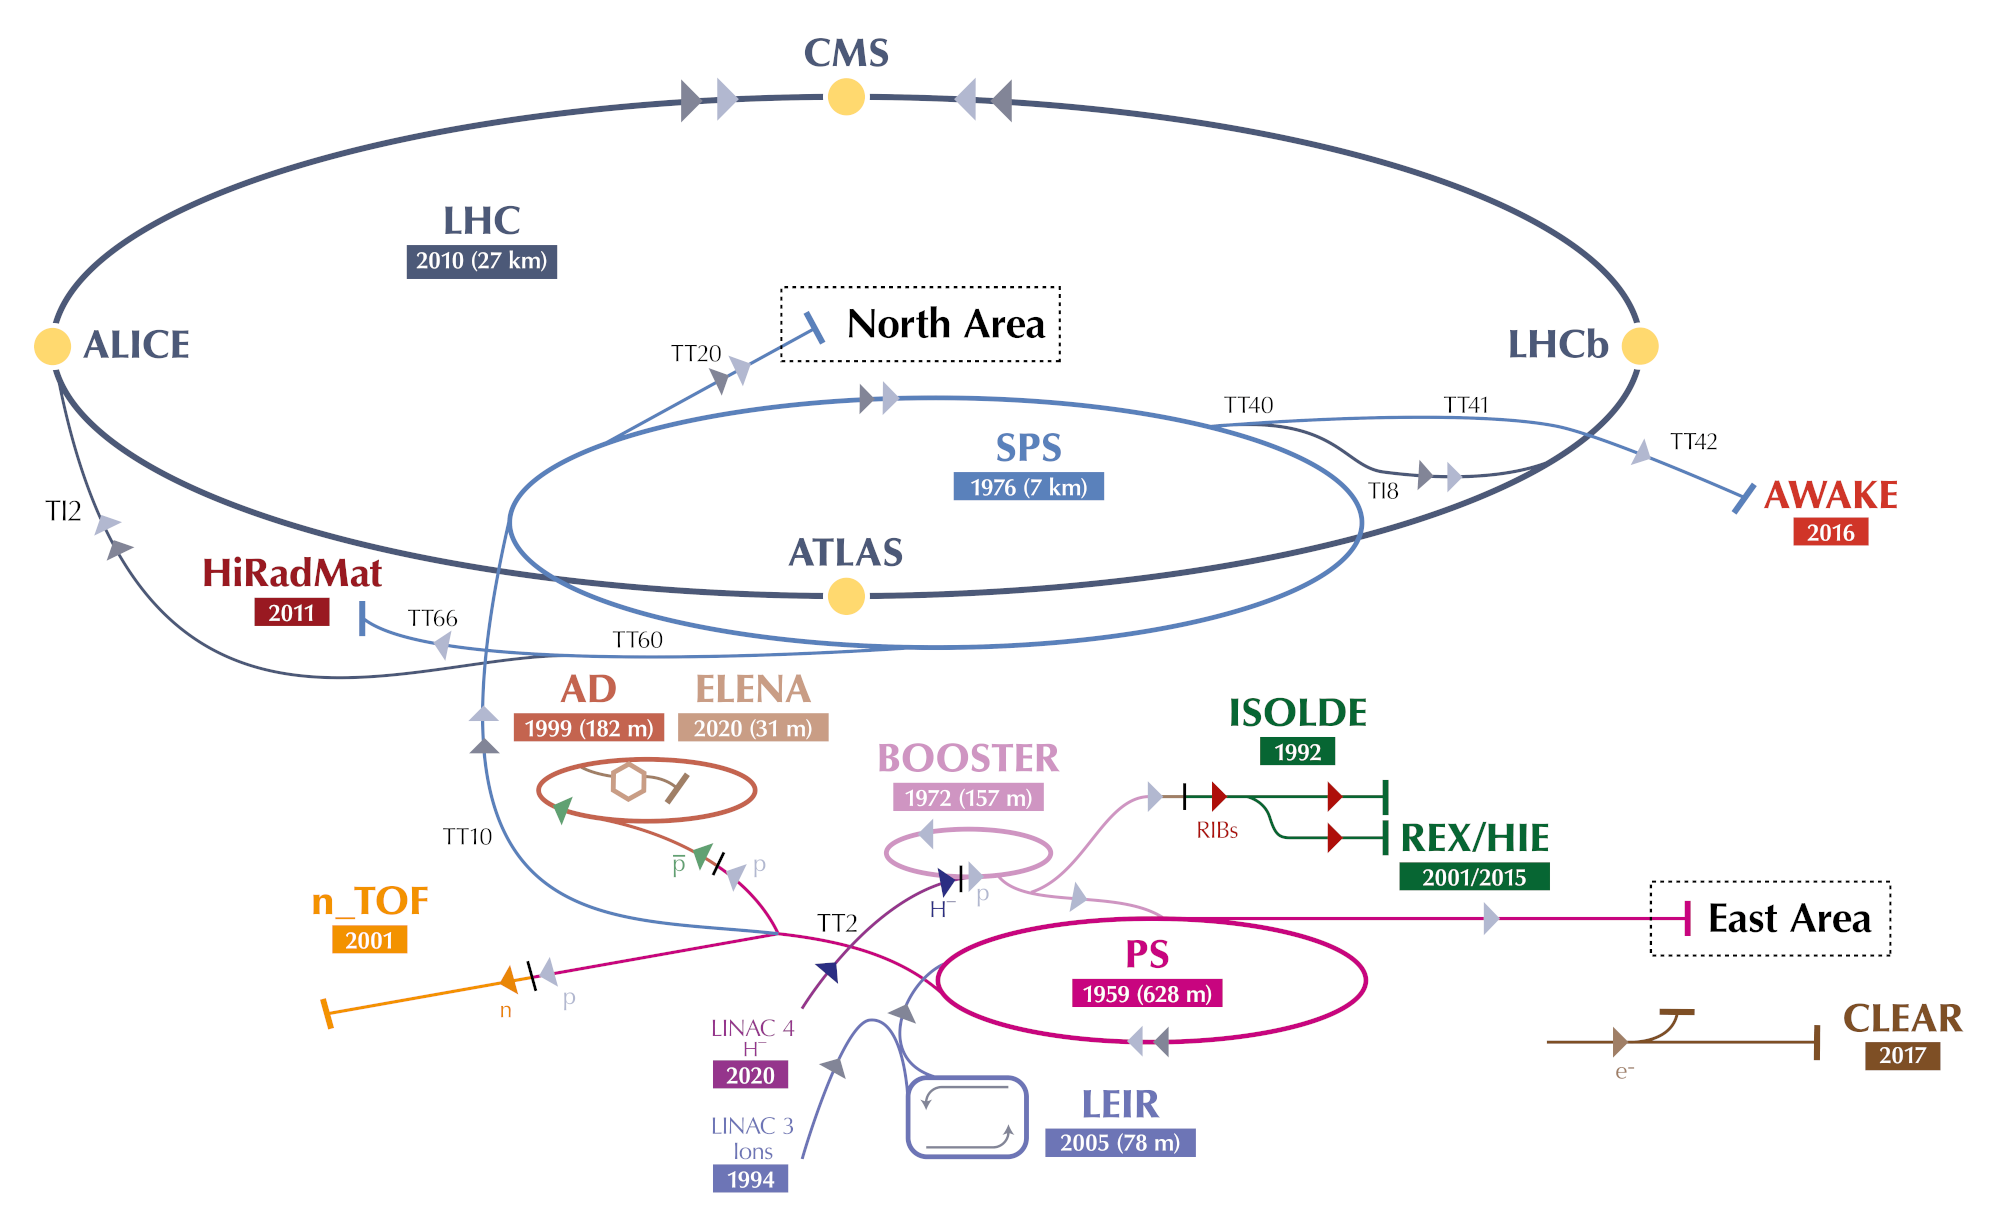
\includegraphics[width=0.9\textwidth, trim=10.5cm 44cm 2cm 20cm,
  %clip]{lhc/cern_complex}
  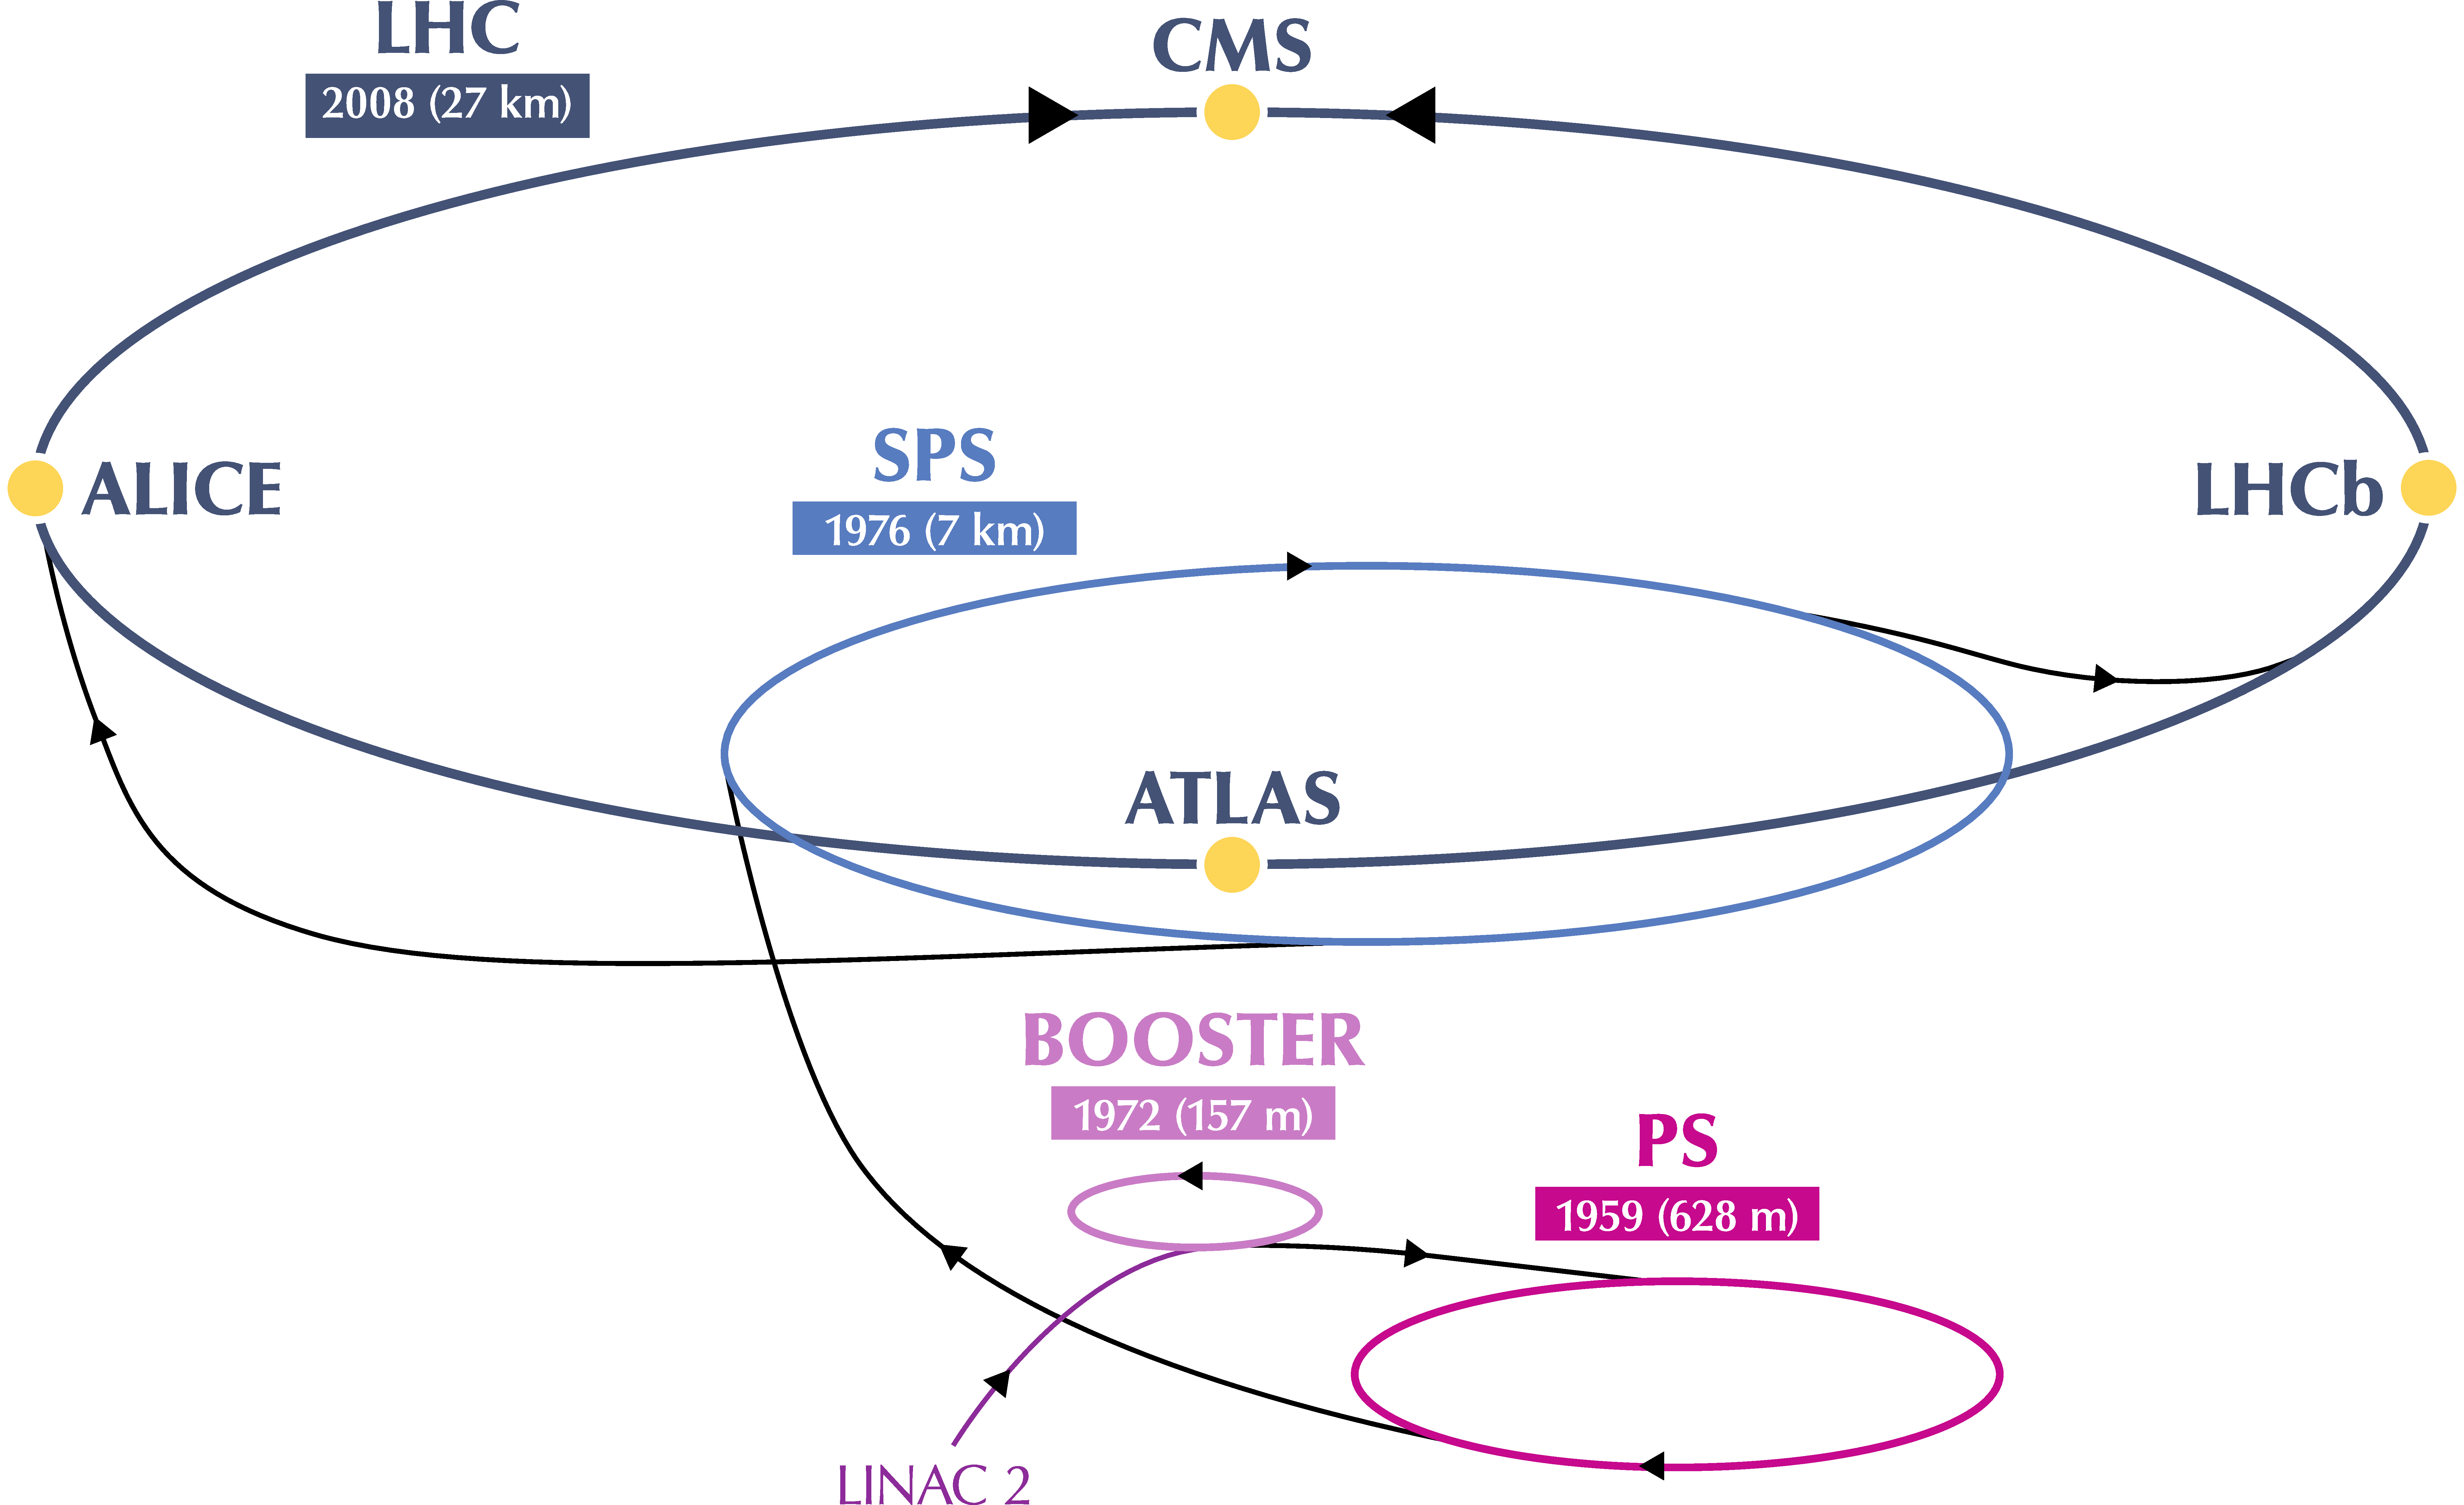
\includegraphics[width=0.75\textwidth]{lhc/cern_complex_trim_otherexp_removed}

  \caption[Illustration of the LHC and its pre-accelerators.]{Illustration of
    the LHC and its pre-accelerators when operating in proton--proton collision
    mode during the data-taking period from 2015--2018 (Run~2). The year of
    first operation and circumference of the accelerators is given in solid
    coloured boxes. The figure is adapted from Ref.~\cite{Mobs:2684277}.}%
  \label{fig:cern_accelerator_complex}
\end{figure}

The main operating period of the LHC started in 2010 with \pp~collisions at
$\sqrt{s} = \SI{7}{\TeV}$. In 2012, the centre-of-mass energy was increased to
\SI{8}{\TeV}. The data-taking period from 2010 to 2012 is referred to as
\emph{Run~1} of the LHC. After extensive upgrades of the LHC and the detectors,
the LHC restarted operation with \pp~collisions at $\sqrt{s} = \SI{13}{\TeV}$ in
\emph{Run~2} which took place from 2015 to 2018. After another shutdown of LHC
and experiments, data-taking recommenced in 2022 with \emph{Run~3}, reaching
unprecedented energy scales of $\sqrt{s} = \SI{13.6}{\TeV}$. At present, Run~3
is foreseen to last until the end of 2025~\cite{lhc_schedule}.

An important performance characteristic of a particle collider is the
instantaneous luminosity, $L$, at a given interaction point. For a process $p$,
the instantaneous luminosity relates the expected number of events from the
process per unit time, $\mathrm{d}N_{p} / \mathrm{d}t$, to the cross section of
the process, $\sigma_{p}$, according to
\begin{align*}
  \frac{\mathrm{d}N_{p}}{\mathrm{d}t} = L \sigma_{p} \,\text{.}
\end{align*}
The expected number of events over a time interval, assuming constant
cross section, is given by $N_{p} = L_{\text{int}} \, \sigma_{p}$, where
$L_{\text{int}} = \int \mathrm{d}t \, L(t)$ is referred to as the integrated
luminosity. When searching for rare physics processes occuring at high-energy
scales, it is typically desirable to perform collisions at the largest,
experimentally feasible $L$ over extensive time periods to maximise the expected
number of events from the rare process.

The integrated luminosity delivered to the ATLAS experiment by the LHC during
Run~2 is shown in \Cref{fig:atlas_int_lumi_vs_time}. In this data-taking period,
the LHC delivered \pp~collisions with an integrated luminosity of about
\SI{156}{\per\femto\barn} of which \SI{139}{\per\femto\barn} pass the
data-quality requirements of the ATLAS experiment~\cite{ATLAS-CONF-2019-021}.
The peak instantaneous luminosity at the IP of the ATLAS experiment ranged from
\SI{0.5e-34}{\per\centi\metre\squared\per\second} at the beginning, to
\SI{1.9e-34}{\per\centi\metre\squared\per\second} at the end of the
Run~2~\cite{ATLAS-CONF-2019-021}. A quantity related to the instantaneous
luminosity is the expected number of inelastic \pp interactions per bunch
crossing, $\mu$. Due to the large cross section of inelastic \pp~collisions at
$\sqrt{s} = \SI{13}{\TeV}$ of about \SI{80}{\milli\barn}~\cite{STDM-2015-05},
multiple interactions occur in a single crossing of the proton bunches. These
interactions contaminate collision events of interest and are referred to as
pile-up. The distribution of $\mu$ is depicted in \Cref{fig:atlas_mu} at the IP
at the ATLAS experiment during Run~2, showing that on average \num{33.7}
inelastic collision events are expected to occur in a single bunch crossing in
the combined Run~2 \pp~collision dataset.

% Luminosity or pile-up plots?
% https://twiki.cern.ch/twiki/bin/view/AtlasPublic/LuminosityPublicResultsRun2

\begin{figure}[htbp]
  \centering

  \begin{subfigure}{0.47\textwidth}
    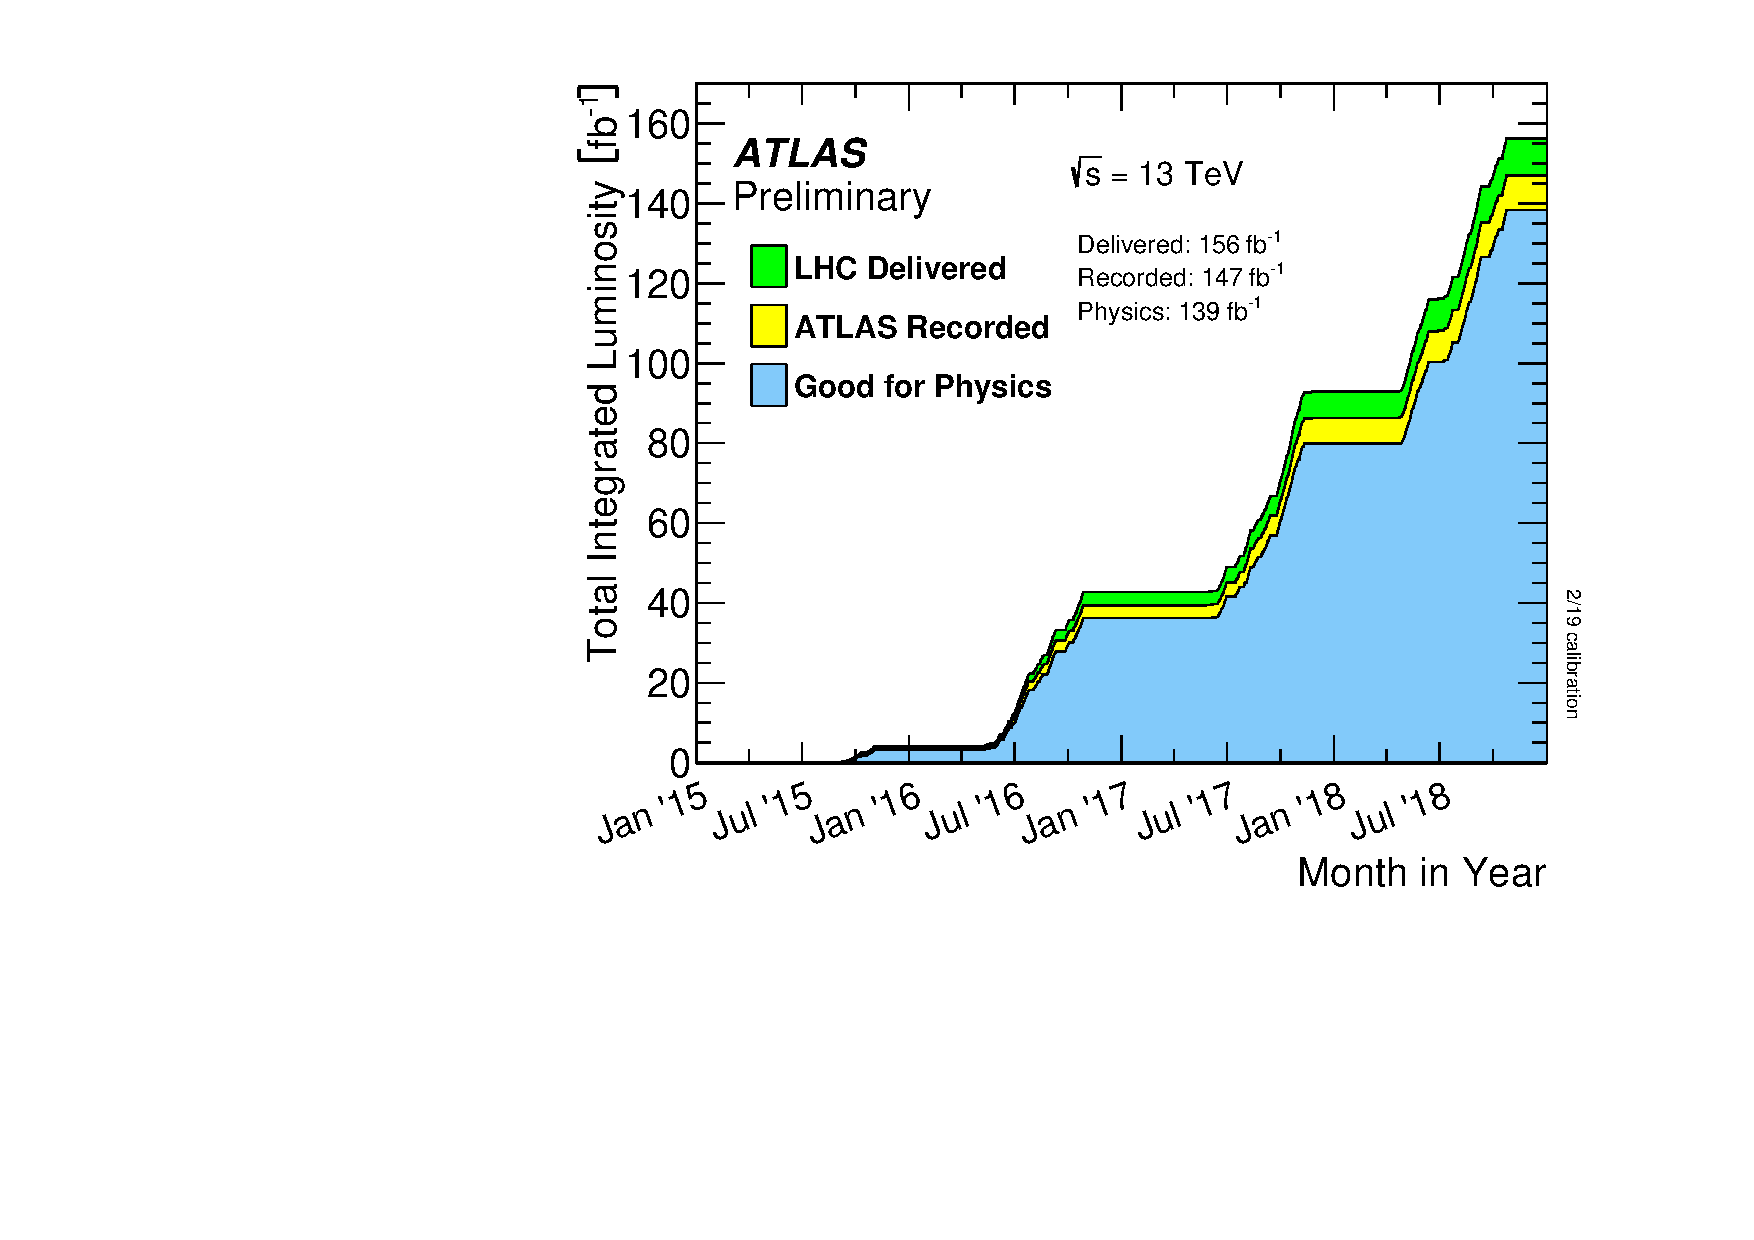
\includegraphics[width=\textwidth]{lhc/int_lumi_vs_time}
    \subcaption{}%
    \label{fig:atlas_int_lumi_vs_time}
  \end{subfigure}\hspace*{0.02\textwidth}%
  \begin{subfigure}{0.47\textwidth}
    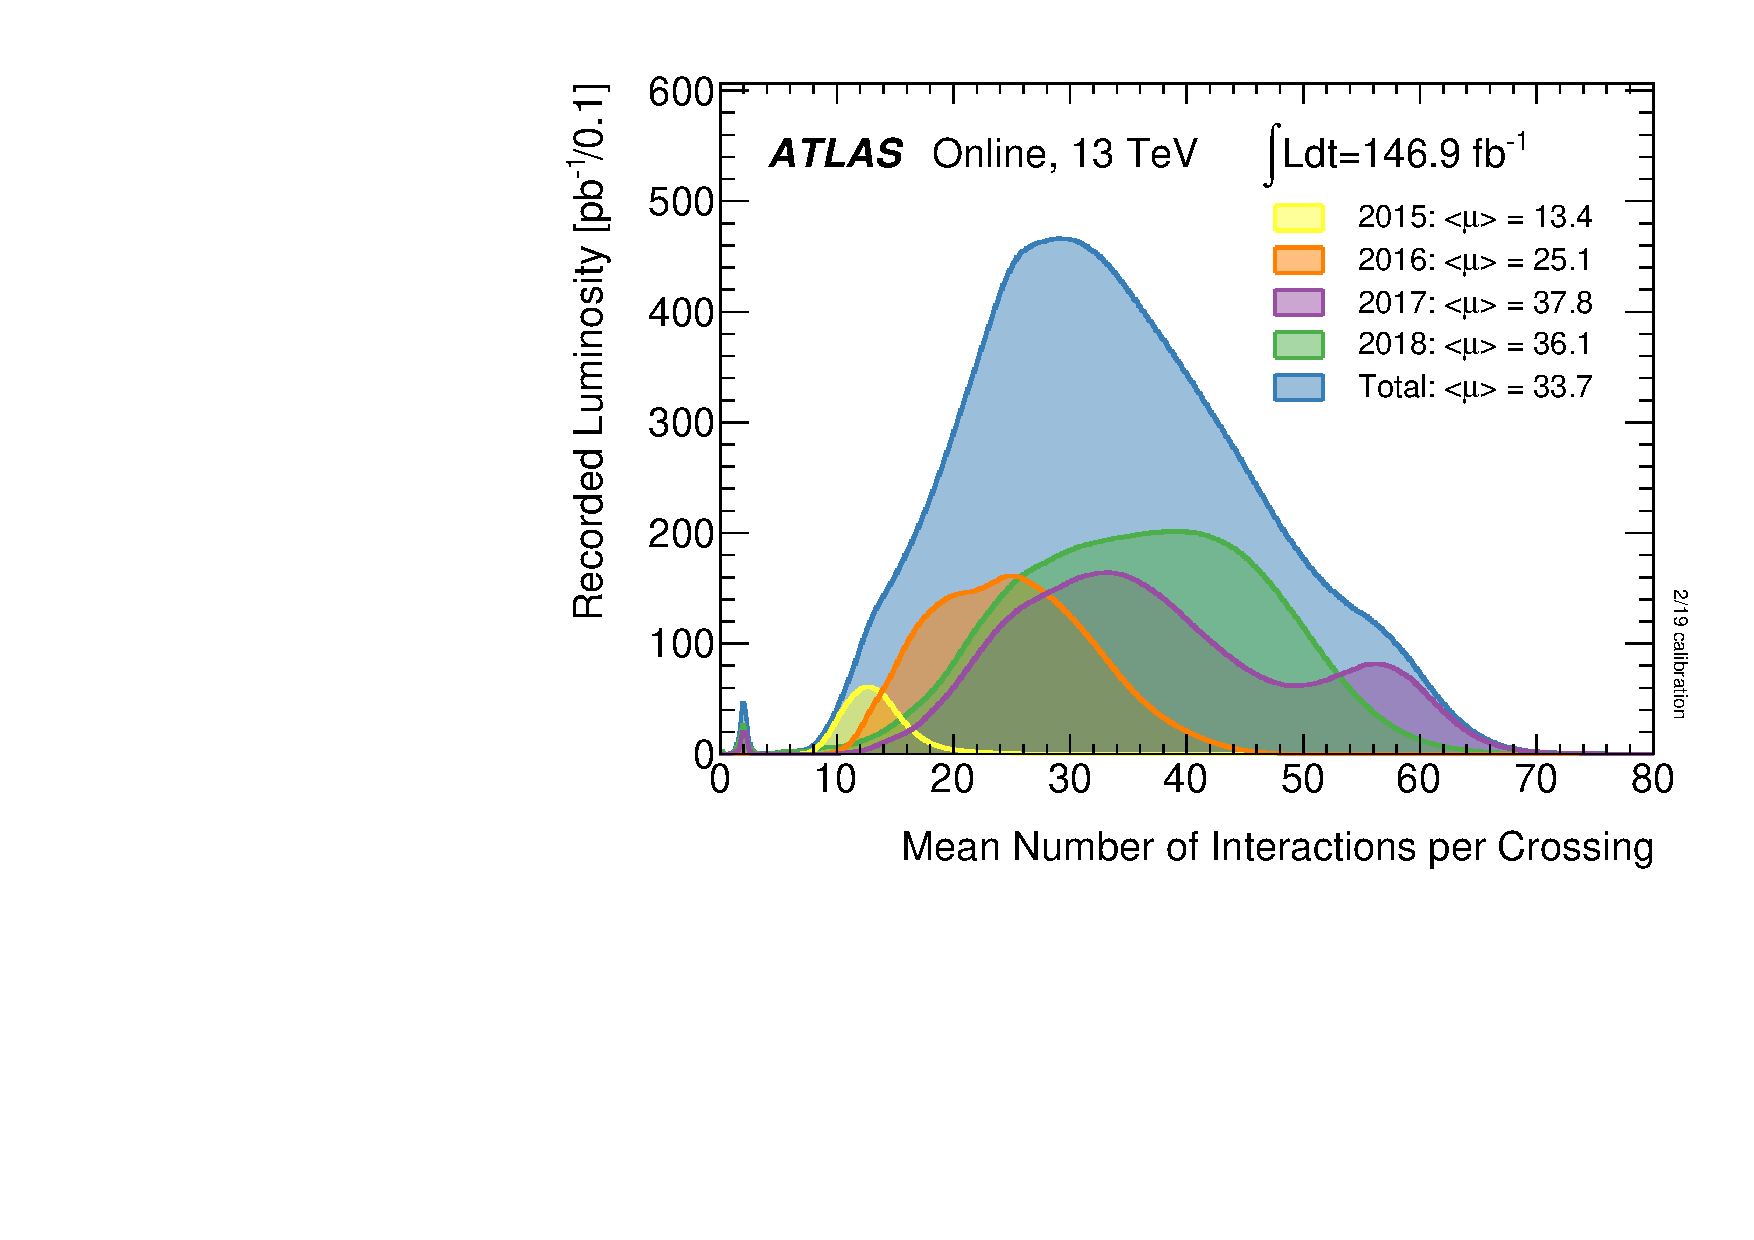
\includegraphics[width=\textwidth]{lhc/mu_2015_2018_fontembed}
    \subcaption{}%
    \label{fig:atlas_mu}
  \end{subfigure}

  \caption[Integrated luminosity and mean number of interactions per bunch
  crossing at the ATLAS experiment during Run~2 of the LHC.]{The integrated
    luminosity as a function of time (a) and the distribution of the mean number
    of interactions per bunch crossing (b) at the ATLAS experiment for
    \pp~collisions during Run~2 of the LHC. In Figure (a), the integrated
    luminosity delivered by the LHC (green), recorded by the ATLAS detector
    (yellow), and passing the data-quality criteria~\cite{DAPR-2018-01} of the
    ATLAS collaboration (blue) is shown. In Figure (b), the mean number of
    interactions per bunch crossing is calculated from the instantaneous
    luminosity assuming an inelastic \pp~collision cross section at
    $\sqrt{s} = \SI{13}{\TeV}$ of \SI{80}{\milli\barn}. The figures are taken
    from Ref.~\cite{atlas_luminosity_summary_plots}.}%
  \label{fig:lumi_and_pu}
\end{figure}

%%% Local Variables:
%%% mode: latex
%%% TeX-master: "../../phd_thesis"
%%% End:

\section{The ATLAS Detector}%
\label{sec:atlas}

The ATLAS detector~\cite{PERF-2007-01}, shown in
\Cref{fig:atlas_detector_overview}, is a cylindrical particle detector
surrounding the LHC beamline at one of the IPs. The detector covers most of the
solid angle around the IP to ensure that all detectable particles from
collisions can be observed. The central part of the ATLAS detector is referred
to as the \emph{barrel}, while the two sections covering the solid angle close
to the LHC beamline are referred to as the \emph{end-caps}. Different layers of
detector technologies are concentrically arranged around the IP that, in
conjunction, allow to detect and identify different types of particles, enabling
an almost full interpretation of collision events.

\begin{figure}[htbp]
  \centering

  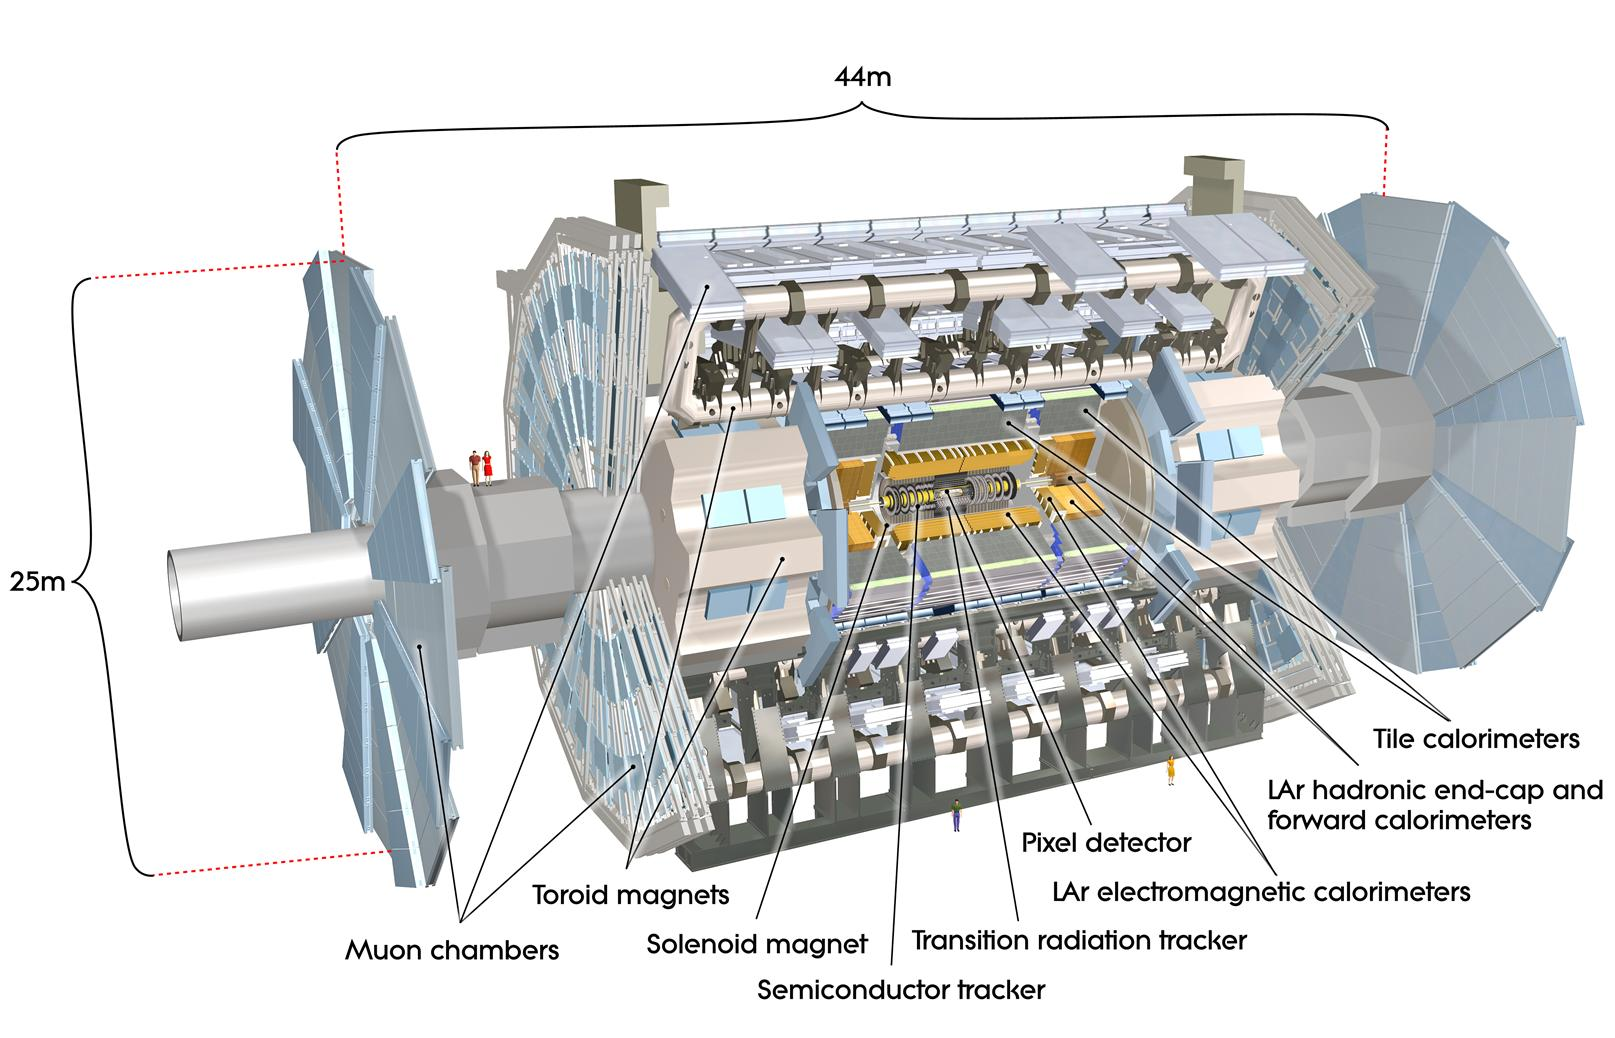
\includegraphics[width=0.76\textwidth]{atlas/atlas_overview}

  \caption{Overview of the ATLAS detector. The image is taken from
    Ref.~\cite{PERF-2007-01}.}%
  \label{fig:atlas_detector_overview}
\end{figure}

The ATLAS experiment uses a right-handed Cartesian coordinate system with the
origin being located in the centre of the detector at the nominal IP. The axes
of the coordinate system are given as follows: the $x$-axis points to the centre
of the LHC, the $y$-axis points upwards, and the $z$-axis points along the LHC
beamline. The plane spanned by the $x$- and $y$-axes is referred to as the
transverse plane. A spherical coordinate system is used to specify directions in
three-dimensional space. The azimuthal angle, $\phi$, of this coordinate system
is defined as the angle in the transverse plane measured with respect to the
$x$-axis, and the polar angle, $\theta$, being the angle with respect to the
$z$-axis. With these coordinate systems, transverse momenta and energies are
defined as $\pT = \sqrt{p_x^2 + p_y^2} = p \sin\theta$ and $\ET = E \sin\theta$,
respectively. At hadron colliders, the polar angle is frequently given in terms
of the pseudorapidity $\eta$, which is defined as
\begin{align*}
  \eta = - \ln\tan\left( \frac{\theta}{2} \right) \,\text{.}
\end{align*}
Similarly, the angular separation between two particles is defined as
\begin{align*}
  \Delta R = \sqrt{\Delta \eta^2 + \Delta \phi^2} \,\text{,}
\end{align*}
where $\Delta \eta$ is the difference in pseudorapidity and $\Delta \phi$ the
smallest azimuthal separation between the particle momenta.

The main components of the ATLAS detector, going from the IP outwards, are the
\emph{Inner Detector} (ID) used for measuring the trajectories of charged
particles, the \emph{Calorimeters} used to destructively measure the energy of
most charged and neutral particles, and the \emph{Muon Spectrometer} (MS) used
to measure the trajectories of muons that can pass the calorimeters. Particles
in the ID are bent in the transverse plane due to a magnetic field of
\SI{2}{\tesla} field strength pointing along the $z$-axis that is produced by a
superconducting solenoid surrounding the ID.  The MS is equipped with
superconducting toroid magnets that bend the trajectories of muons in the
direction described by the $\eta$-coordinate. The curvature of charged particle
trajectories in the ID and MS allows to determine the sign of the electric
charge and momentum of particles. The following sections summarise the
sub-systems of the ATLAS detector.


\subsection{The Inner Detector}

The ID, schematically depicted in \Cref{fig:atlas_inner_detector}, is the
innermost part of the ATLAS detector. It performs non-destructive measurements
of the trajectories of charged particles within $|\eta| < 2.5$ by measuring the
points where charged particles cross active detector layers. The measurement of
several points on the trajectory, and the known magnetic field in the ID, allows
to reconstruct the trajectory of the particle. The reconstructed trajectory is
referred to as the \emph{charged-particle track} and often abbreviated as
\emph{track}. The precise measurement of charged-particle tracks is important to
reconstruct the primary vertex (PV) of the hard interaction with high spatial
resolution, allowing to remove tracks from pile-up which are typically displaced
from the PV along the $z$-axis. Moreover, the accurate reconstruction of
secondary vertices, i.e.\ displaced vertices originating from decays of unstable
particles produced in the hard interaction, is crucial to identify jets
originating from $b$-quarks.% which hinges on the precision of the track
% reconstruction in the ID.

\begin{figure}[htbp]

  \begin{subfigure}[b]{0.55\textwidth}
    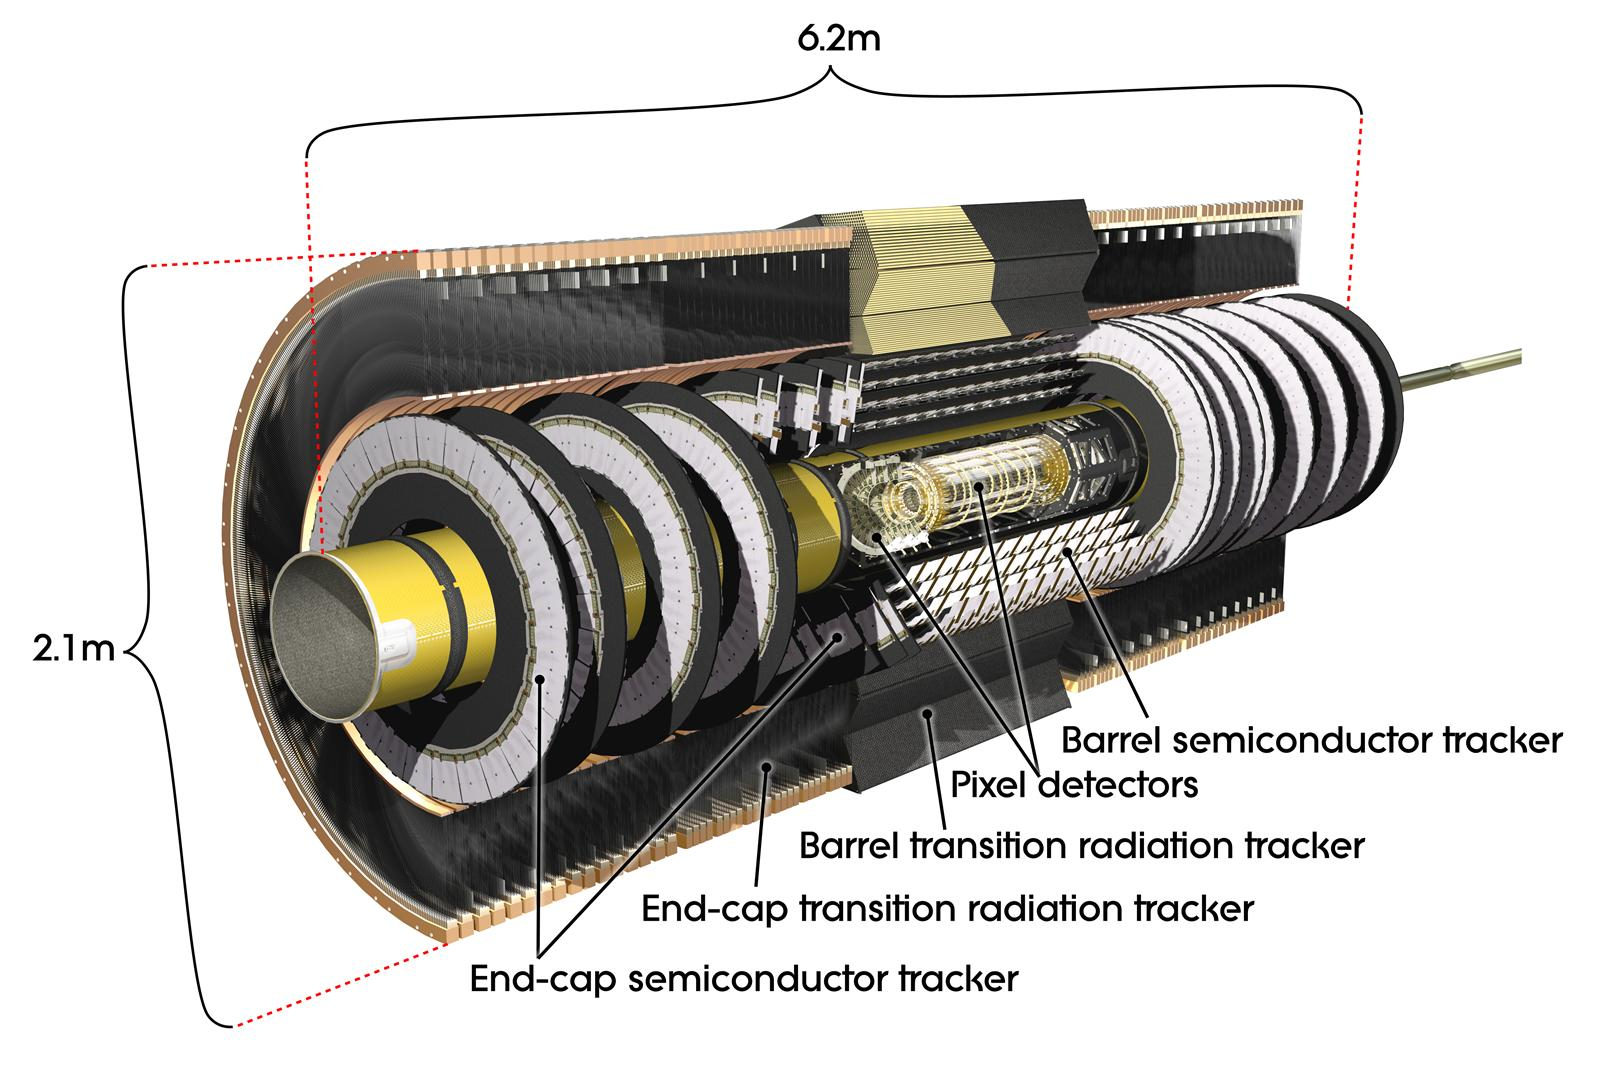
\includegraphics[width=\textwidth]{atlas/atlas_indet_1}%
    \subcaption{}
  \end{subfigure}\hfill%
  \begin{subfigure}[b]{0.45\textwidth}
    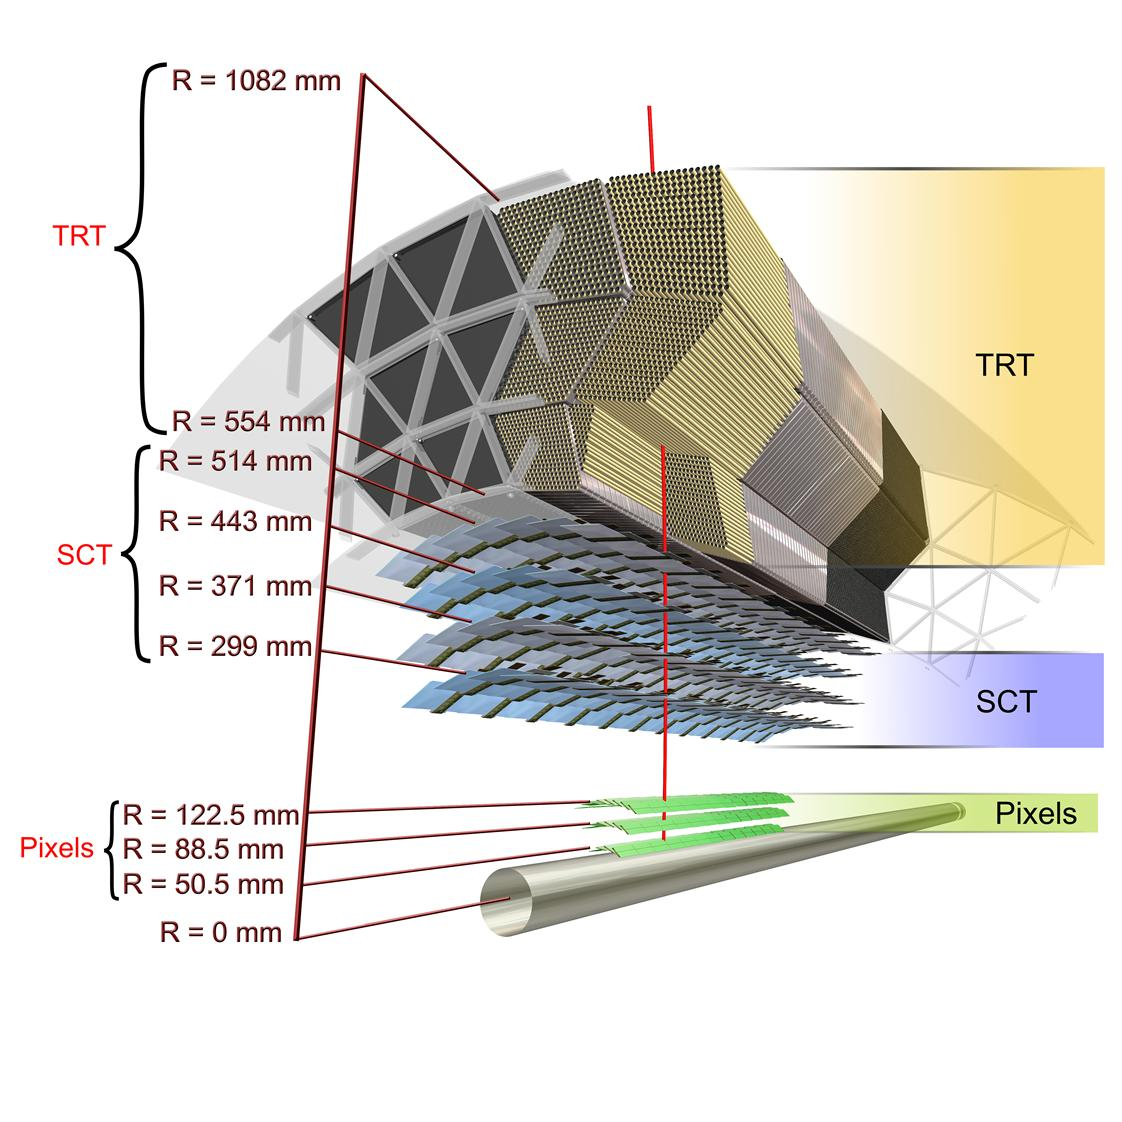
\includegraphics[width=\textwidth, trim=0 2.5cm 0 1cm,
    clip]{atlas/atlas_indet_2}%
    \subcaption{}%
    \label{fig:indet_barrel}
  \end{subfigure}

  \caption{Schematic view of the ID including the two end-caps (a). A zoomed in
    view of the barrel region of the ID (b). The Insertable B-Layer (IBL), which
    was introduced into the ATLAS detector after Run~1 of the LHC, is not
    displayed. The IBL is located closest to the beampipe at a radius of
    $r = \SI{33.5}{\milli\metre}$~\cite{ATLAS-TDR-19,PIX-2018-001}. The images
    are taken from Ref.~\cite{PERF-2007-01}.}%
  \label{fig:atlas_inner_detector}
\end{figure}

The requirements on the tracking system vary with the distance from the IP.
Closest to the IP, tracking detectors with high-granularity are required for the
reconstruction of primary and secondary vertices that can operate in a
high-radiation environment. At larger distances, the particle flux is
significantly reduced and the requirements on the spatial resolution relaxed.
Therefore, different detector technologies are used to cover the needs of the
tracking system in a cost-effective manner.

% Pixel
The ID sub-system closest to the beampipe are the pixel detectors located at
distances of \SIrange{33.5}{122.5}{\milli\metre} from the beamline in the barrel
region of the ATLAS detector (cf.\ \Cref{fig:atlas_inner_detector}). The pixel
detectors are based on semiconductor technology with an active detector area
that is segmented into a grid of rectangular elements, referred to as
pixels. These pixels have size of \SI{50}{\micro\metre} in the transverse
direction and \SIrange{250}{400}{\micro\metre} along the
beamline~\cite{PERF-2007-01,PIX-2018-001}. A charged particle traversing the
pixel detector ionises the active detector material leading to the deposition of
electric charge in nearby pixels. The charge deposited in individual pixels can
be read out to determine the point where the particle crossed the detector
layer. The pixel detectors are arranged in four layers concentric with the
beamline in the barrel region and three disks per end-cap region. Particles
produced at the IP typically traverse four layers of pixel detectors within the
acceptance of $|\eta| < 2.5$ of the tracking system.

% SCT
The pixel detector is surrounded by the \emph{Semiconductor Tracker} (SCT)
covering radii of \SIrange{299}{514}{\milli\metre} from the beamline in the
barrel region (cf.\ \Cref{fig:atlas_inner_detector}). Similar to the pixel
detector, the SCT is based on semiconductor detector technology, however, the
active detector area is segmented in long but thin strips (microstrips) with a
pitch between strips of about \SI{80}{\micro\metre}~\cite{PERF-2007-01}. A
single microstrip detector layer only provides a position measurement in the
plane perpendicular to the strips. Therefore, SCT modules consist of two layers
of microstrips which are tilted by a small angle to resolve the ambiguity in the
direction parallel to the strips. The SCT is arranged in four layers in the
barrel and nine disks in the end-cap region, yielding at least four measurements
for tracks within the acceptance of the tracking system~\cite{PERF-2007-01}.

% TRT
The \emph{Transition Radiation Tracker} (TRT) is the final layer of the ID
covering radii of \SIrange{554}{1082}{\milli\metre} (cf.\
\Cref{fig:atlas_inner_detector}), however, with reduced acceptance of
$|\eta| < 2.0$ compared to the semiconductor-based trackers. The TRT consists of
about \num{300000} straw-tube chambers, which are gaseous ionisation detectors,
with a diameter of \SI{4}{\milli\metre} arranged in up to 73 layers in the
barrel region and 160 planes in the end-caps~\cite{PERF-2007-01}. The straw-tube
chambers determine the radius at which an ionising particle passed through the
tube, however, no position information parallel to the straw-tubes is obtained.
% The straw-tube chambers consist of gas-filled, electrically conductive tubes
% serving as cathodes with an anode wire passing through the centre of the
% tubes. Charged particles passing through the tubes ionise the gas, the
% resulting electrons/ions being accelerated towards the anode/cathode.
The straw-tubes of the TRT are interleaved with polypropylene fibres (foils) in
the barrel (end-cap) region~\cite{PERF-2007-01}. These fibres/foils provide
interfaces between different dielectric media at which ultrarelativistic
particles can emit transition radiation in the form of
X-rays~\cite{Grupen:2008zz}. At the energies of particles produced at the ATLAS
experiment, the emission of transition radiation is only relevant for electrons
and positrons. The X-rays emitted by electrons/positrons at the interfaces are
absorbed in the xenon-based gas-mixture\footnote{Selected drift tubes affected
  by gas leaks are operated using a cheaper, argon-based gas
  mixture~\cite{IDET-2015-01}.} inside the straw-tubes, leading to measurably
higher ionisation compared to a charged particle passing through the drift
tube. This sensitivity of the TRT to transition radiation is used to identify
electrons and positrons.
% Proportional to the Lorentz factor and thus most relevant for light particles.

\subsection{The Calorimeter System}%
\label{sec:atlas_calorimeters}


The ATLAS calorimeter system, schematically depicted in
\Cref{fig:atlas_calorimeters}, surrounds the ID and is used to perform
destructive measurements of the energy of most charged and neutral particles. Of
the particles predicted by the SM, only muons and neutrinos can traverse the
ATLAS calorimeter system without being absorbed. The calorimeter system covers a
pseudorapidity range of $|\eta| < 4.9$, thus instrumenting almost the full solid
angle surrounding the IP. This is important to prevent detectable particles from
avoiding detection, which consequently allows to determine the sum of transverse
momentum carried away by undetectable particles such as neutrinos or non- or
only weakly-interacting particles from BSM theories, the so-called missing
transverse momentum (\Cref{sec:atlas_met}).

\todo[inline]{Calorimetry is complementary to charged-particle tracking. Energy
  / momentum resolution and dependency on E / p.}

\begin{figure}[htbp]
  \centering

  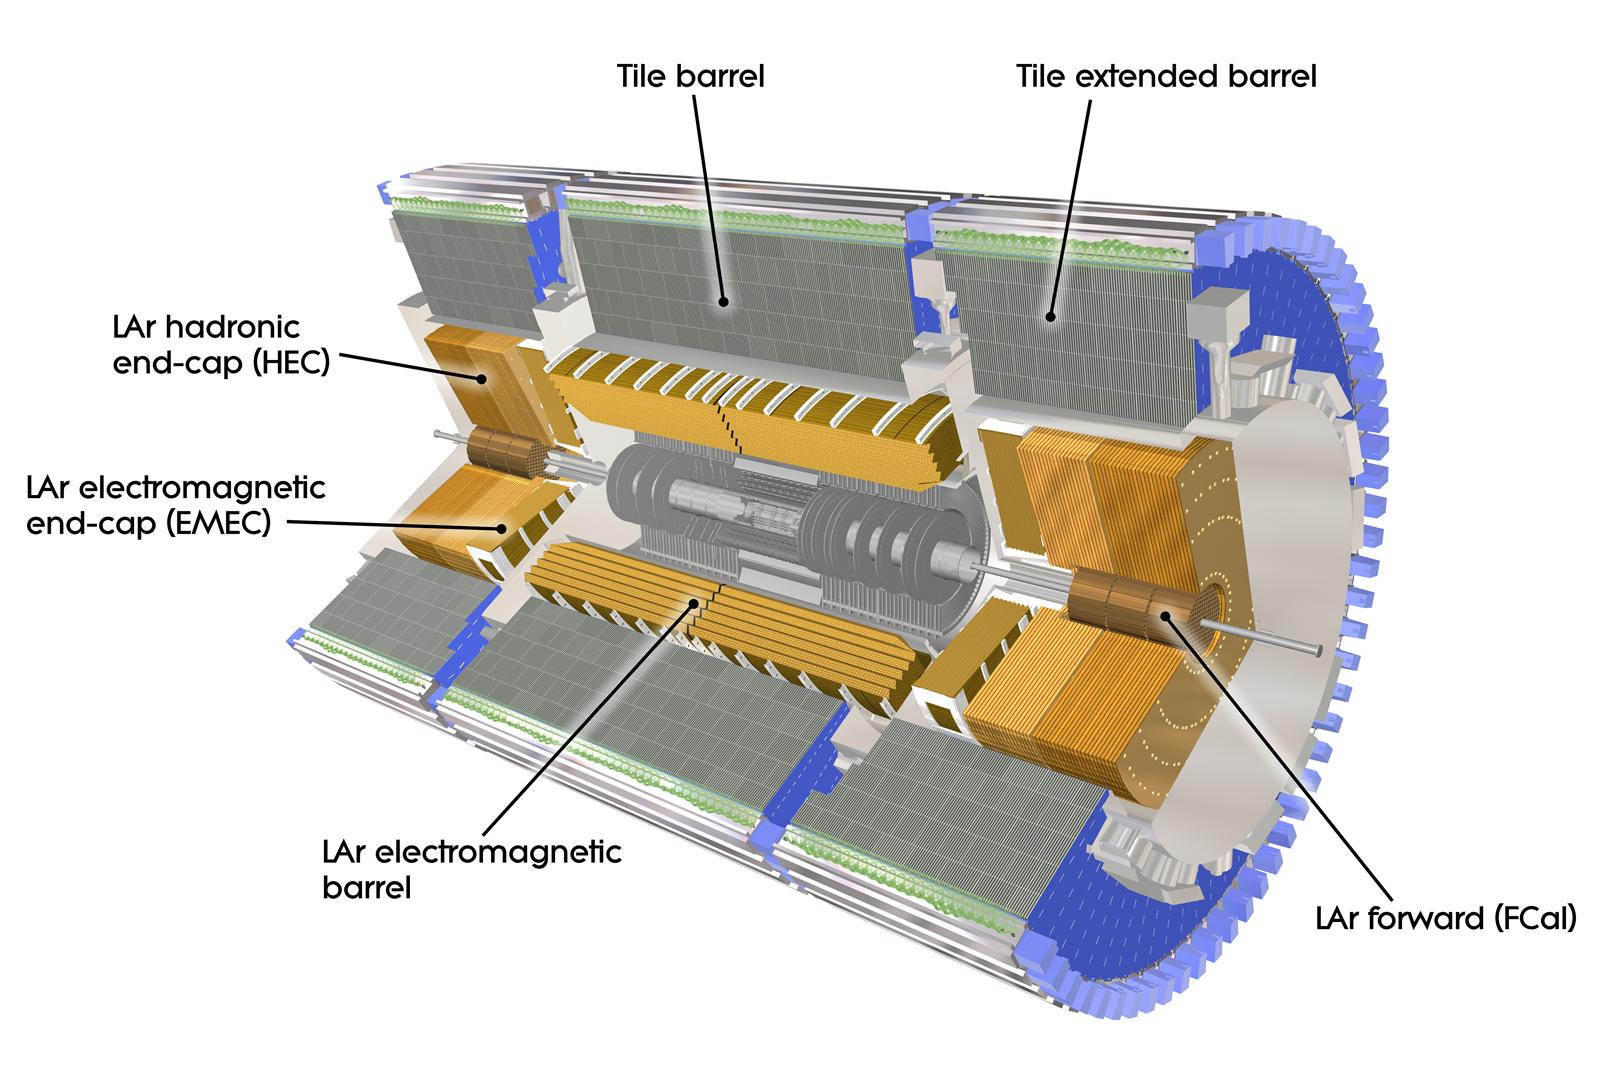
\includegraphics[width=0.65\textwidth]{atlas/atlas_calo}

  \caption{Overview of the ATLAS calorimeter system. The image is taken from
    Ref.~\cite{PERF-2007-01}.}%
  \label{fig:atlas_calorimeters}
\end{figure}

The ATLAS calorimeter is split into two major parts. The \emph{electromagnetic
  calorimeter}, the innermost part of the calorimeter, is used to measure the
energies of electrons/positrons and photons. It is followed by the
\emph{hadronic calorimeter} which measures the energy of charged and neutral
hadrons that are able to pass through the electromagnetic calorimeter. This
design is governed by the interactions of particles with matter at the energy
scales relevant for the ATLAS experiment. Highly energetic electrons/positrons
and photons interact with the calorimeter material by emitting Bremsstrahlung
and converting into electron--positron pairs, respectively. This process occurs
repeatedly, producing a cascade of electrons, positrons, and photons, until the
energy of the constituent particles is sufficiently small to be absorbed in the
material. These cascades, referred to as \emph{electromagnetic showers}, are
homogeneous and compact with high energy density. The dimensions of the
electromagnetic calorimeters are chosen such that they fully contain
electromagnetic showers originating from promptly produced electrons/positrons
and photons. The interactions of hadrons with the calorimeter material are
driven by nuclear interactions which also result in cascades of secondary
particles. A variety of processes are relevant for the evolution of these
so-called \emph{hadronic showers}, for example: inelastic scattering of hadrons
at nuclei, spallation, fission, or neutron
capture~\cite{Kolanoski:2016gyf}. Moreover, electromagnetic showers are an
important sub-component of hadronic showers which, for example, originate from
photons produced in $\pi^0$ decays. The length scales of hadronic showers are
larger, both laterally and longitudinally, than the ones of electromagnetic
showers.
% Moreover, hadronic showers show localised fluctuations distinguishing them from
% the homogenous electromagnetic showers.
This is reflected in the design of the ATLAS calorimeter system with the
hadronic calorimeter having almost four times the radial thickness of the
electromagnetic calorimeter~\cite{ATLAS-TDR-02,ATLAS-TDR-03}.

The electromagnetic and hadronic calorimeters are sampling calorimeters, i.e.\
they consist of alternating layers of absorber material for shower development
and active detector layers that sample the shower as it develops. Depending on
the part of the calorimeter, the active detector layers are either ionisation
chambers filled with liquid argon (LAr) or plastic scintillator tiles connected
to photomultiplier tubes.


\subsubsection{Electromagnetic Calorimeters}

The electromagnetic calorimeter of the ATLAS detector (cf.\
\Cref{fig:atlas_calorimeters}) is divided into a barrel ($|\eta| < 1.475$),
end-cap ($1.375 < |\eta| < 3.2$), and forward ($3.1 < |\eta| < 4.9$)
region~\cite{PERF-2007-01}. The electromagnetic calorimeters in the barrel and
end-cap region consist of lead absorbers with LAr-filled gaps that are
instrumented with electrodes to form ionisation chambers. The calorimeter is
segmented both laterally and longitudinally, with varying granularity, to
provide information on the location and shape of showers in the calorimeter. The
forward electromagnetic calorimeter uses copper absorbers and a single
longitudinal layer instead.
% Additionally, the region of $|\eta| < 1.8$ in front
% of the calorimeter is instrumented with a so-called pre-sampler, which is a
% thin layer of LAr-based calorimeter used to


\subsubsection{Hadronic Calorimeters}

The hadronic calorimeter (cf.\ \Cref{fig:atlas_calorimeters}) is divided into a
barrel ($|\eta| < 1.0$), extended barrel ($0.8 < |\eta| < 1.7$), end-cap
($1.5 < |\eta| < 3.2$), and forward ($3.1 < |\eta| < 4.9$)
region~\cite{PERF-2007-01}.  The barrel and extended barrel calorimeter consists
of alternating steel plates and plastic scintillator tiles. The scintillators
are connected via optical fibres to photomultiplier tubes for readout. The
hadronic end-cap calorimeter (HEC) and forward calorimeter consist of LAr-filled
ionisation chambers with copper and tungsten absorbers, respectively. The
hadronic calorimeter is also segmented laterally and longitudinally, although
with reduced granularity compared to the electromagnetic calorimeter.


\subsection{The Muon Spectrometer}%
\label{sec:atlas_ms}

The MS, shown in \Cref{fig:atlas_muon_system}, is the outermost and largest part
of the ATLAS detector. It is a tracking detector providing independent momentum
measurements of muons that pass the calorimeters. The active detector elements
of the MS are based on gaseous ionisation detectors for cost-effective
instrumentation of large areas. The MS provides a coverage of $|\eta| < 2.7$ for
precision tracking and $|\eta| < 2.4$ for triggering on muons.

\begin{figure}[htbp]
  \centering

  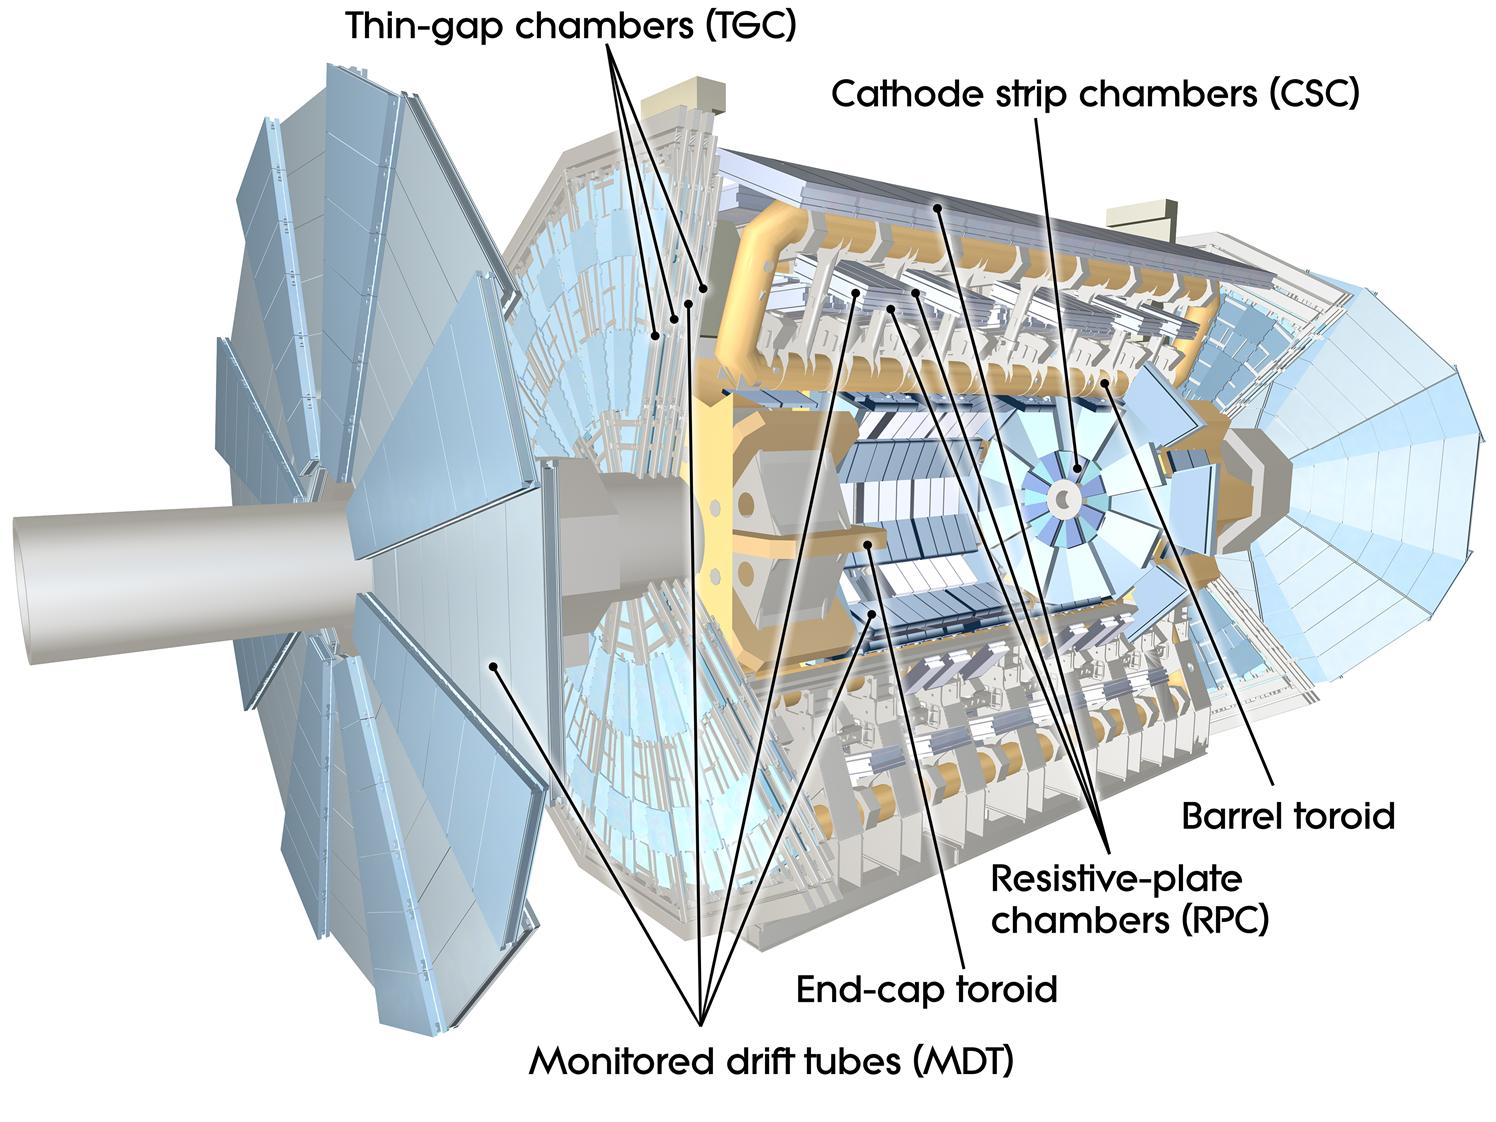
\includegraphics[width=0.56\textwidth]{atlas/atlas_muon}

  \caption{Overview of the ATLAS muon spectrometer. The image is taken from
    Ref.~\cite{PERF-2007-01}.}%
  \label{fig:atlas_muon_system}
\end{figure}

The ATLAS detector uses multiple layers monitored drift tube
chambers\footnote{Deformations of the muon chambers are actively monitored using
  an optical alignment system built into the frame of the chambers.} (MDTs) for
precision tracking in $|\eta| < 2.7$. To cope with the large rate of incident
particles in the forward region, the innermost layer in $2.0 < |\eta| < 2.7$ is
replaced by cathode strip chambers (CSCs). The MS is complemented with resistive
plate chambers (RPCs) and thin gap chambers (TGCs) in the barrel
($|\eta| < 1.05$) and end-cap ($1.05 < |\eta| < 2.7$) region, respectively,
providing the necessary timing information to identify the bunch crossing a muon
originates from. The MS is arranged, as depicted
in~\Cref{fig:atlas_muon_system}, in three cylindrical layers surrounding the LHC
beamline in the barrel region. A gap in the instrumentation of the MS is left at
$\eta = 0$ for access to the inner parts of the detector for servicing. The
end-cap region is instrumented by muon chambers in the form of three wheels
perpendicular to the beampipe. A \emph{small wheel} is located in front of the
end-cap toroid, and two \emph{big wheels} are located behind the end-cap
toroid. Every layer/wheel consists of multiple tracking planes.


\subsection{The ATLAS Trigger System}%
\label{sec:atlas_trigger}

With a peak bunch crossing rate of \SI{40}{\mega\hertz} and an expected number
of inelastic \pp-collisions in a single bunch crossing of around \num{30} (cf.\
\Cref{fig:lumi_and_pu}), it is not possible to record every collision event due
to limitations in the detector read-out and data storage. However, most
collision events are not of particular interest to the physics programme of the
ATLAS experiment. For example, events containing a weak vector boson decaying
into leptons are expected to occur about once every $10^6$ inelastic
\pp-collisions at $\sqrt{s} = \SI{13}{\TeV}$~\cite{STDM-2015-03}. Other
processes, such as the production of Higgs bosons, are multiple orders of
magnitude less frequent than the production of $Z$ and $W$ bosons.

The task of the ATLAS trigger system~\cite{TRIG-2019-04} is to reduce the rate
at which events are recorded by performing an event pre-selection already during
data-taking (\emph{online}). This is achieved by monitoring the ATLAS detector
for signatures of rare physics processes, for example indicated by the presence
of charged leptons with large transverse momenta. A multitude of different event
selections, usually referred to as \emph{triggers}, are implemented in the ATLAS
trigger system to target the signatures of different physics processes. The
implementation of these triggers are heavily constrained due to the limited
detector read-out and strict latency and bandwidth constraints. Due to the
increasing instantaneous luminosity during Run~2 of the LHC, the triggers
employed by the ATLAS experiment had to evolve to meet the bandwidth
requirements. Therefore, the exact selections of triggers targeting particular
signatures changed as Run~2 progressed. During Run~2, the ATLAS trigger system
reduced the rate of selected events to about
\SI{1.2}{\kilo\hertz}~\cite{TRIG-2019-04} which could be recorded for
(\emph{offline}) analysis.

The ATLAS trigger system consists of two stages. The first stage, called the
Level-1 (L1) trigger, implements the event selection in hardware using custom
electronic circuits. At the L1 trigger, only calorimeter and MS information with
reduced granularity can be used for selection. The rate of accepted events is
reduced to \SI{100}{\kilo\hertz}~\cite{TRIG-2019-04} by the L1 trigger. If an
event is accepted, all sub-detectors of the ATLAS experiment are read-out and
the data are sent to the second stage of the trigger system, the so-called
High-Level Trigger (HLT). The HLT is software-based and runs reconstruction
algorithms similar to those applied during offline event reconstruction.  Event
selections at the HLT are staged into \emph{chains} of algorithms with
increasing computational/time complexity. A given HLT chain is only applied to
events selected by particular L1 triggers, usually referred to as the L1 seed of
the chain. The selections applied by the HLT reduces the mean rate of accepted
events to the target of \SI{1.2}{\kilo\hertz}~\cite{TRIG-2019-04}.


%%% Local Variables:
%%% mode: latex
%%% TeX-master: "../../phd_thesis"
%%% End:

\section{Reconstruction of Collision Events in the ATLAS Detector}%
\label{sec:object_reco_at_atlas}

\todo[inline]{Introductory sentence}

Omissions: Photons, special reconstruction techniques for certain analyses


\subsection{Tracking and Vertexing}

The reconstruction of trajectories of charged particles is referred to as track
reconstruction or tracking. The inputs to the track reconstruction in the ID of
the ATLAS detector are \emph{space-points} from the pixel and SCT detector, and
\emph{drift circles} from the TRT. Space-points are measurements of location in
three-dimensional space obtained by clustering the charge signals of adjacent
segments in the pixel and SCT detectors. Drift circles are measurements of
distance from the anode wires of individual straw-tubes in the TRT derived from
electron drift times in the straw-tubes.

Track reconstruction employs pattern recognition techniques to select
space-points and drift circles that are compatible with the hypothesis of a
charged particle in the axial magnetic field of the ID. Least-squares fits are
performed, using selected space-points and drift circles, to determine the
parameters characterising the track at a reference point. This reference point
is typically the point of closest approach (perigee) to the nominal beam-spot
position in the transverse plane. Five parameters describe the track at the
perigee. The transverse (longitudinal) distance of the perigee from the
reference point given by $d_0$ ($z_0$), also referred to as the transverse
(longitudinal) impact parameter of the track. The azimuthal and polar angle of
the track at the perigee given by $\phi$ and $\theta$, respectively. Finally,
the ratio of electric charge and transverse momentum, $q / \pT$, parameterises
the curvature of the track.

At the ATLAS experiment, two primary tracking algorithms are used which are
referred to as the \emph{inside-out} and \emph{outside-in}
algorithms~\cite{Cornelissen:2007vba,Salzburger:2015sgq,PERF-2015-08}. The
inside-out algorithm starts by reconstructing tracks in the pixel and SCT
detector only, then extending the track using measurements in the TRT. In
contrast, the outside-in algorithm starts with the reconstruction of track
segments in the TRT which are them combined with space-points from the pixel and
SCT detectors. The outside-in algorithm is used to improve the reconstruction
efficiency for tracks from secondary particles, such as electrons produced in
conversions of photons in the detector material, for which the inside-out
algorithm can fail to reconstruct a track.

Reconstructed tracks are used to determine the locations of inelastic scattering
interactions between protons in the ATLAS detector. These locations are marked
by multiple charged-particle tracks originating from the same point in the
detector and are referred to as primary vertices (PVs). Consequently, the vertex
of the hard scattering interaction of interest and the associated particles can
be identified, allowing to reject reconstructed objects originating from
pile-up. The ATLAS primary vertex reconstruction~\cite{PERF-2015-01} finds and
reconstructs PVs using an iterative fitting procedure. The PV reconstruction
starts by reconstructing a vertex at the location of highest track density in
$z_0$ with respect to the beam-spot position. An adaptive vertex
fitter~\cite{Fruhwirth:2007hz} is used to iteratively determine the vertex
position while weighting reconstructed tracks according to their compatibility
with the vertex position. After the fit, tracks that are incompatible with the
vertex position are considered as unassociated and the process is repeated on
all unassociated tracks. Finally, the PV with the largest sum of $\pT^2$ of
associated tracks that has at least two tracks with $\pT > \SI{500}{\MeV}$ is
selected as the PV of the hard scattering interaction of interest. Other
vertices with at least two associated tracks are considered as originating from
pile-up~\cite{PERF-2015-01}.


\subsection{Topological Clustering of Energy in Calorimeter Cells}

The segmentation of the calorimeters in lateral and longitudinal direction
allows to reconstruct the three-dimensional shape of electromagnetic and
hadronic showers. These showers typically extend over multiple cells in the
calorimeter, thus requiring the combination of several cells to fully
reconstruct a shower. The ATLAS experiment uses a \emph{topological calorimeter
  cell clustering algorithm}~\cite{PERF-2014-07} to combine the signals of
locally connected cells passing certain signal thresholds, thereby suppressing
noise from the calorimeter electronics and pile-up. These clusters of
calorimeter cells, referred to as topo-clusters, are used to reconstruction
electromagnetic and hadronic showers in the calorimeters. Due to fluctuations in
the shower development and calorimeter noise, multiple topo-clusters are
typically required to fully reconstruct the calorimeter response to a single
particle.

The ATLAS calorimeter has a different response to electromagnetic and hadronic
showers, i.e.\ the calorimeter is \emph{non-compensating}. By default, the
energies of topo-clusters are calibrated assuming the response originates from
an electromagnetic shower (EM scale). However, the development of
electromagnetic and hadronic showers leads to differences in their shower
shapes, as previously discussed in \Cref{sec:atlas_calorimeters}. This is
exploited by the \emph{local hadronic calibration}~\cite{PERF-2014-07} which
uses shower shape information of individual topo-clusters to determine their
likely origin and apply electromagnetic and hadronic calibrations that are
weighted accordingly. The energy scale of topo-clusters after the local hadronic
calibration is referred to as the LC scale.

Topo-clusters are used as inputs for the reconstruction of higher-level physics
objects in the ATLAS detector. For example, topo-clusters at EM and LC scale are
used in the reconstruction of electrons and \tauhadvis, respectively, which is
discussed in \Cref{sec:ele_rec,sec:tau_rec}.


\subsection{Electrons}%
\label{sec:ele_rec}

The reconstruction of electrons (and positrons) in the ATLAS detector exploits
their characteristic signature of a charged-particle track in the ID pointing
towards a narrow cluster of energy in the electromagnetic calorimeter. The
reconstruction of electrons in the region of $|\eta| < 2.47$ and excluding the
transition regions between the barrel and end-caps, $1.37 < |\eta| < 1.52$, is
described in the following based on
Refs.~\cite{ATL-PHYS-PUB-2017-022,EGAM-2018-01}.

Electron reconstruction is seeded by topo-clusters (EM scale) that have more
than \SI{50}{\percent} of their energy located in cells of the electromagnetic
calorimeter, which are referred to as EM topo-clusters. In addition,
topo-clusters are only considered if the transverse energy in the
electromagnetic part of the calorimeter, $\ET^{\text{EM}}$, exceeds
\SI{400}{\MeV}. A first attempt of geometrically matching the EM topo-cluster to
an ID track is made. If the EM topo-cluster cannot be matched to a
well-reconstructed track but has a longitudinal and lateral shower shape similar
to the signature of an electron, then a second pass of tracking is performed in
a region surrounding the cluster. The second pass allows for up to
\SI{30}{\percent} of energy loss at each intersection with detector material due
to the emission of bremsstrahlung. After an ambiguity resolution scheme in case
multiple tracks match the cluster, the cluster is required to be geometrically
matched to a single track. EM topo-clusters with matched tracks are considered
as seeds for a \emph{supercluster} reconstruction algorithm if the cluster
fulfils $\ET^{\text{EM}} > \SI{1}{\GeV}$ and the matched track passes
reconstruction quality criteria. \emph{Satellite clusters}, which are EM
topo-clusters in the vicinity of the supercluster seed, are included in the
supercluster to account for electromagnetic showers being reconstructed as
multiple topo-clusters or the formation of additional clusters from electrons
emitting bremsstrahlung. After applying initial calibrations and corrections to
supercluster, the track matching is repeated using the supercluster barycentre
instead of the barycentre of the EM topo-cluster seed. Finally, multivariate
calibrations of the electron energy and corrections from comparisons of
reconstructed electrons in data and simulation are
applied~\cite{PERF-2017-03,EGAM-2018-01}.

Electrons that are promptly produced in the hard scattering reaction are often
of interest for physics analyses. Other sources of reconstructed electron
candidates are quark- or gluon-initiated jets that mimic the signature of an
electron, or electrons from secondary sources such as hadron decays or photon
conversions. \emph{Identification} and \emph{isolation} requirements can be
applied to select promptly produced electrons and reject electron candidates
from other sources. Electron identification is performed using a
likelihood-based classifier exploiting variables sensitive to the shower shape,
reconstruction quality of the matched track, information about transition
radiation emission in the TRT, and spatial and momentum matching between the
track and the supercluster~\cite{EGAM-2018-01}. Furthermore, in most event
topologies little detector activity is expected in the vicinity of promptly
produced electrons. Therefore, isolation variables are defined that quantify the
activity in an area surrounding the electron candidate using reconstructed
tracks and topo-clusters in the calorimeters~\cite{EGAM-2018-01}. Selections are
applied on these isolation variables to further reject backgrounds originating
from jets and non-prompt electrons.


\subsection{Muons}%
\label{sec:muon_rec}

The reconstruction of muons in the ATLAS experiment primarily targets the
signature of a particle that leaves a track in the ID and MS with only minimal
energy deposition in the calorimeters due to ionisation. The instrumentation of
the MS (cf.~\Cref{sec:atlas_ms}) allows for the reconstruction of muons up to
$|\eta| < 2.7$. The following description of the muon reconstruction is based on
Ref.~\cite{MUON-2018-03}.

A stand-alone reconstruction of tracks in the MS is attempted by first
reconstructing straight-line segments in individual layers of the MS. Track
candidates are constructed from multiple track segments compatible with the
signature of the trajectory of a muon produced at the interaction point. These
candidates seed a precision fit to obtain the full muon trajectory and the
associated parameters in the MS.

Different reconstruction techniques are employed yielding five different types
of reconstructed muons~\cite{MUON-2018-03}:
\begin{description}

\item[Combined muons] are reconstructed by matching a track in the MS to a track
  in the ID. A combined fit of the ID and MS track is performed, accounting for
  the ionisation energy loss of muons in the calorimeters, to reconstruct the
  muon trajectory. Within $2.5 < |\eta| < 2.7$, combined muons may be
  reconstructed using short segments of ID tracks instead of fully reconstructed
  ID tracks.

\item[Inside-out muons] are reconstructed by extending a track in the ID with
  additional hits in the MS, the additional hits being used for a combined fit
  of the muon trajectory in the ID and MS. The inside-out strategy aims to
  recover cases where the stand-alone track reconstruction in the MS fails to
  find a track.

\item[MS extrapolated muons] are reconstructed by extrapolating a stand-alone MS
  track to the beamline in cases where no matching ID track is found. This
  strategy improves the reconstruction efficiency of muons outside of the ID
  tracking acceptance, i.e.\ $2.5 < |\eta| < 2.7$.

\item[Segment-tagged muons] are reconstructed by matching an ID track
  extrapolated to the MS to one or more short track segments in the MS. The muon
  four-momentum is reconstructed using the parameters of the ID track.

\item[Calorimeter-tagged muons] are reconstructed from ID tracks leaving a
  calorimeter signature similar to a minimum ionising particle. The ID track
  defines the four-momentum of calorimeter-tagged muons.

\end{description}
Several muon identification working points are defined using these muon types
and additional requirements on the quality of the ID and MS tracks, and
compatibility of ID and MS tracks in terms of charge and momentum. In this
thesis, the \emph{loose} and \emph{medium} working points are used and
summarised hereafter. Of these working points, the medium working point has the
most stringent requirements on the quality of reconstructed muons. It requires
muons to be reconstructed as combined or inside-out muons or, alternatively, MS
extrapolated muons in $2.5 < |\eta| < 2.7$ to improve the reconstruction
efficiency outside of the acceptance of ID track reconstruction. The
\emph{loose} working point augments the medium working point by additionally
allowing segment- and calorimeter-tagged muons in $|\eta| < 0.1$, a region with
a gap in the MS instrumentation (cf.~\Cref{sec:atlas_ms}), and relaxing the MS
track quality requirements applied to inside-out muons. Muons passing the
\emph{loose} working point are a superset of muons passing the \emph{medium}
working point.

\todo[inline]{Cosmic muons and TTVA? Muon momentum corrections measured in
  data~\cite{PERF-2015-10}.}

Isolation requirements are applied to reconstructed muon candidates to
distinguish prompt from non-prompt muons. A similar approach to the one adopted
for electrons, previously discussed in \Cref{sec:ele_rec}, is used.


\subsection{Jets and $b$-tagging}%
\label{sec:jet_rec}

The production of quarks and gluons in hard scattering interactions leads to the
development of collimated sprays of particles which are referred to as
jets. Jets are produced as a result of the colour confinement in QCD, leading to
a fragmentation of the initial quark/gluon until the energy of the resulting
fragments is sufficiently small to bind into colourless hadrons. The primary
constitutents of jets are charged/neutral hadrons and photons from hadron
decays. To reconstruct the kinematic properties of the quark/gluon that
initiated the jet, the four-momenta of all particles from the
fragmentation/hadronisation process have to be collected. This task is addressed
by jet algorithms which combine particles, or other entities, into clusters to
reconstruct jets. In the ATLAS experiment, the anti-\kt jet clustering
algorithm~\cite{Cacciari:2008gp} is most frequently used.


\subsubsection{The Anti-\kt Jet Clustering Algorithm}

The anti-\kt jet clustering algorithm operates on collections of entities with
well-defined four-momenta (e.g.\ topo-clusters in the calorimeters). Any set of
one or more entities can be viewed as a pseudo-jet with a four-momentum given by
the sum of the constituent four-momenta. Pseudo-jets are sequentially combined
if they are close according to a distance metric. The distance between the
pseudo-jets $i$ and $j$ is defined by the anti-\kt algorithm
as~\cite{Cacciari:2008gp}
\begin{align*}
  d_{ij} &= \min\bigl( p_{\text{T}i}^{-2}, p_{\text{T}j}^{-2} \bigr)
           \frac{ \dRy(i, j)^2 }{ R^2 } \,\text{,}
\end{align*}
where $\pT$ refers to pseudo-jet transverse momentum,
$\dRy = \sqrt{\Delta y^2 + \Delta \phi^2}$ is the distance of two pseudo-jets in
the $y\phi$-plane, with $y$ being the rapidity of the pseudo-jet,\footnote{The
  rapidity is defined as
  $y = \frac{1}{2} \ln \left( \frac{E + p_z}{E - p_z} \right)$, where $E$ is
  then energy of a particle and $p_z$ the momentum component along the
  beamline. In the ultrarelativistic limit the rapidity is equivalent to the
  pseudo-rapidity.} and $R$ is the jet-radius parameter of the algorithm. A
stopping criterion for the clustering algorithm is provided by the distance
$d_{i\text{B}} = p_{\text{T}i}^{-2}$ by proceeding as
follows~\cite{Cacciari:2008gp}:
\begin{enumerate}
\item Find the minimum distance $d_{ij}$ for all pairs of pseudo-jets and the
  minimum distance $d_{i\text{B}}$ for all pseudo-jets.

\item If $\min_{i,j}(d_{ij}) < \min_{i}(d_{i\text{B}})$: The pair of pseudo-jets
  corresponding to the minimum in $d_{ij}$ is combined to form a new pseudo-jet.

\item If $\min_{i,j}(d_{ij}) \geq \min_{i}(d_{i\text{B}})$: The pseudo-jet
  yielding the minimum $d_{i\text{B}}$ is declared as a jet and removed from the
  procedure.
\end{enumerate}
These steps are repeated until no pseudo-jets are left.

The anti-\kt algorithm produces conical jets with a typical radius of $\dRy = R$
provided no high-\pT emissions are located in the vicinity of the jet. The
algorithm has desirable theoretical properties, such as reconstructed jets being
insensitive to soft or collinear emissions, thus making it the choice of the
default jet clustering algorithm in the ATLAS experiment. In this thesis, the
jet clustering uses the anti-\kt algorithm with a jet-radius parameter of
$R = 0.4$. The implementation of the \textsc{FastJet} library~\cite{Fastjet} is
used.


\subsubsection{Jet Reconstruction using Particle Flow}

% The inputs to the jet algorithm are provided by a particle flow reconstruction
% algorithm, described in Refs.~\cite{PERF-2015-09,JETM-2018-05}, exploiting the
% superior momentum resolution of the tracking system for charged particles with
% low transverse momenta by replacing the calorimetric measurement of their
% energy with a tracking-based momentum measurement, necessitating the
% subtraction of energy deposits by charged particles in the calorimeter. The
% particle flow algorithm provides an improved jet energy and angular resolution
% as well as pile-up stability compared to jets constructed based on topological
% clusters in the calorimeters (at EM scale)
% only~\cite{PERF-2015-09,JETM-2018-05}.

Earlier analyses performed by the ATLAS collaboration used jets reconstructed by
applying the anti-\kt algorithm to topo-clusters in the calorimeters,
disregarding any information about charged particles from the tracking
system. New techniques combining information from tracking and calorimetry are
adopted by the ATLAS experiment for the reconstruction of jets. These are based
on a reconstruction algorithm referred to as \emph{particle
  flow} that attempts to reconstruct individual
charged and neutral particles from their detector signatures.

Jet reconstruction based on particle flow, described in
Refs.~\cite{PERF-2015-09,JETM-2018-05}, exploits the superior energy and angular
resolution of reconstructing low-\pT charged hadrons using their track in the ID
compared to a calorimetric measurement.\footnote{The charged pion mass is
  assumed for the relationship between the momentum and energy of charged
  particles in the tracker.} Neutral particles have to be reconstructed from
topo-clusters in the calorimeter, making it necessary to subtract the energy
deposited by charged hadrons to prevent double-counting. This subtraction is
performed by the particle flow algorithm to reconstruct neutral particles in the
form of \emph{neutral particle flow objects}. Similarly, charged hadrons
reconstructed from their track in the ID are referred to as \emph{charged
  particle flow objects}.  Charged and neutral particle flow objects are used as
inputs to the anti-\kt jet clustering algorithm to reconstruct jets used for
physics analyses.

Jet reconstruction using particle flow has several advantages compared to a
calorimeter-based approach, as detailed in Ref.~\cite{PERF-2015-09}. The energy
resolution for jets at low transverse momenta
($\pT^{\text{jet}} \lessapprox \SI{50}{\GeV}$, see for example
Ref.~\cite{JETM-2018-05}) is improved due to the inclusion of tracking
information. In part, this is due to the ability to account for charged hadrons
with transverse momenta down to \SI{500}{\MeV} in the reconstruction of jets. In
comparison, calorimeter-based jet reconstruction has shortcomings in accounting
for low-\pT charged hadrons due to charged hadrons being bent out of the jet
clustering cone, or their calorimeter signals being suppressed by the
topo-cluster algorithm. Moreover, jets reconstructed using particle flow are
less susceptible to pile-up since charged particle flow objects can be
associated to the PV of the hard interaction using the reconstructed tracks.


\subsubsection{$b$-tagging}

The production of $b$-quarks is an important signature of rare physics processes
produced at the LHC. Similar to other quarks except the top quark, a $b$-quark
produced in a hard interaction leads to the formation of a jet, referred to as a
$b$-jet. A distinct feature of $b$-jets is the presence of a $b$-hadron with a
mass exceeding \SI{5}{\GeV}~\cite{pdg2020} in the jet. These $b$-hadrons are
short-lived and will, after traversing a short but measurable distance in the
ATLAS detector, decay via the weak interaction. For example, the lightest
$B$-mesons, the $B^0$ and $B^\pm$, have proper lifetimes of about
\SI{1.5e-12}{\second}~\cite{pdg2020} and thus, assuming a $B$ meson momentum of
\SI{10}{\GeV}, a mean flight path of approximately \SI{1}{\milli\metre} before
decaying. Decays of $b$-hadrons frequently produce final states containing
$c$-hadrons, which also decay after traversing a short distance in the detector.

The task of identifying $b$-jets is referred to as $b$-tagging. Features
resulting from displaced decays of $b$- and $c$-hadrons can be exploited for the
purpose of $b$-tagging. The $b$-tagging algorithms used as part of this thesis
use two categories of features:
\begin{description}

\item[Track impact parameter based:] Due to the relatively large mass of
  $b$-hadrons, the daughter particles of displaced $b$-hadron decays are
  produced at an angle with respect to the initial flight direction of the
  $b$-hadron. Consequently, the tracks of the daughter particles tend to have
  larger longitudinal and transverse track impact parameters with respect to the
  PV of the hard interaction compared to promptly produced charged
  particles. The deviation of an impact parameter from zero is quantified in
  terms of the \emph{impact parameter significance} by dividing the impact
  parameter by its uncertainty.

\item[Secondary vertex based:] Secondary vertices resulting from the daughter
  particles of $b$- and $c$-hadron decays can be reconstructed using charged
  particle tracks measured in the ID. Among others, the displacement of the
  reconstructed secondary vertex from the PV of the hard interaction or the
  invariant mass of the charged particles associated to the vertex can be used
  as features in $b$-tagging.

\end{description}

The $b$-tagging algorithms used at the ATLAS experiment combine discriminants
provided by multiple low-level algorithms. In this thesis, the \textsc{DL1r}
$b$-tagging algorithm~\cite{FTAG-2019-07-001} is used that combines the outputs
of five algorithms using neural networks:
\begin{description}

\item[IP2D \& IP3D] The \textsc{IP2D} and \textsc{IP3D}
  algorithms~\cite{ATL-PHYS-PUB-2017-013} provide $b$-tagging discriminants
  based on likelihood-ratio classifiers constructed from the distribution of
  impact parameter significances in $b$-, $c-$, and \emph{light}-jets. While
  \textsc{IP2D} only considers the distribution of the transverse impact
  parameter significance of tracks, \textsc{IP3D} considers the joint
  distribution of transverse and longitudinal impact parameter significances.
  In both cases, the likelihoods of all tracks in the jet are combined by
  neglecting any dependencies of the impact parameters between tracks.

\item[RNNIP] The \textsc{RNNIP} algorithm~\cite{ATL-PHYS-PUB-2017-003} extends
  the idea of \textsc{IP2D} and \textsc{IP3D} by also considering dependencies
  of impact parameter significances between tracks associated to a jet. This is
  accomplished with a recurrent neural network taking tracks of the jet as
  inputs. Track properties, such as the impact parameter signficances, are
  passed to the network with every track. Based on these inputs, \textsc{RNNIP}
  estimates the probability of the jet being a $b$-, $c$-, or \emph{light}-jet.

\item[SV1 \& JetFitter] The \textsc{SV1}~\cite{ATL-PHYS-PUB-2017-011} and
  \textsc{JetFitter}~\cite{ATL-PHYS-PUB-2018-025} algorithms reconstruct the
  secondary vertices resulting from the displaced decays of $b$- and
  $c$-hadrons. While \textsc{SV1} reconstructs a single secondary vertex,
  \textsc{JetFitter} attempts to reconstruct the cascade of $b$- and $c$-hadron
  decays with two secondary vertices. The secondary vertices determined by both
  algorithms are used to define discriminating variables that are provided to
  the high-level $b$-tagging algorithms. Examples of these variables are the
  invariant mass of the tracks associated to the vertices or the significance of
  the distance between the secondary vertex and the PV of the hard interaction.

\end{description}
The \textsc{DL1r} $b$-tagging algorithm combines these discriminants with basic
kinematic properties of the jet to yield a high-level $b$-tagging discriminant.
Selections on this discriminant define several $b$-tagging working points with
different probabilities of correctly identifying a $b$-jet, referred to as the
$b$-tagging efficiency.
% \SI{60}{\percent}, \SI{70}{\percent}, \SI{77}{\percent} and \SI{85}{\percent}


\subsection{Tau Leptons}%
\label{sec:tau_rec}

The \taulepton has a mass of \SI{1.777}{\GeV}~\cite{pdg2020} and is therefore
sufficiently massive to decay into final states with charged leptons or hadrons
as is illustrated in \Cref{fig:tau_feynman}. These decay modes are referred to
as leptonic (\taulep) and hadronic (\tauhad) decay modes, respectively.

\todo[inline]{Come back to this once I know what has to be introduced here.}

The \taulepton decay and branching ratios are illustrated in
\Cref{fig:tau_branching_ratios}.

% - What is \taulep and \tauhad
% - How are \taulep reconstructed?
% - What is the difference between \tauhad and \tauhadvis


\begin{figure}[htb]
  \begin{subfigure}[b]{0.47\textwidth}
    \centering

    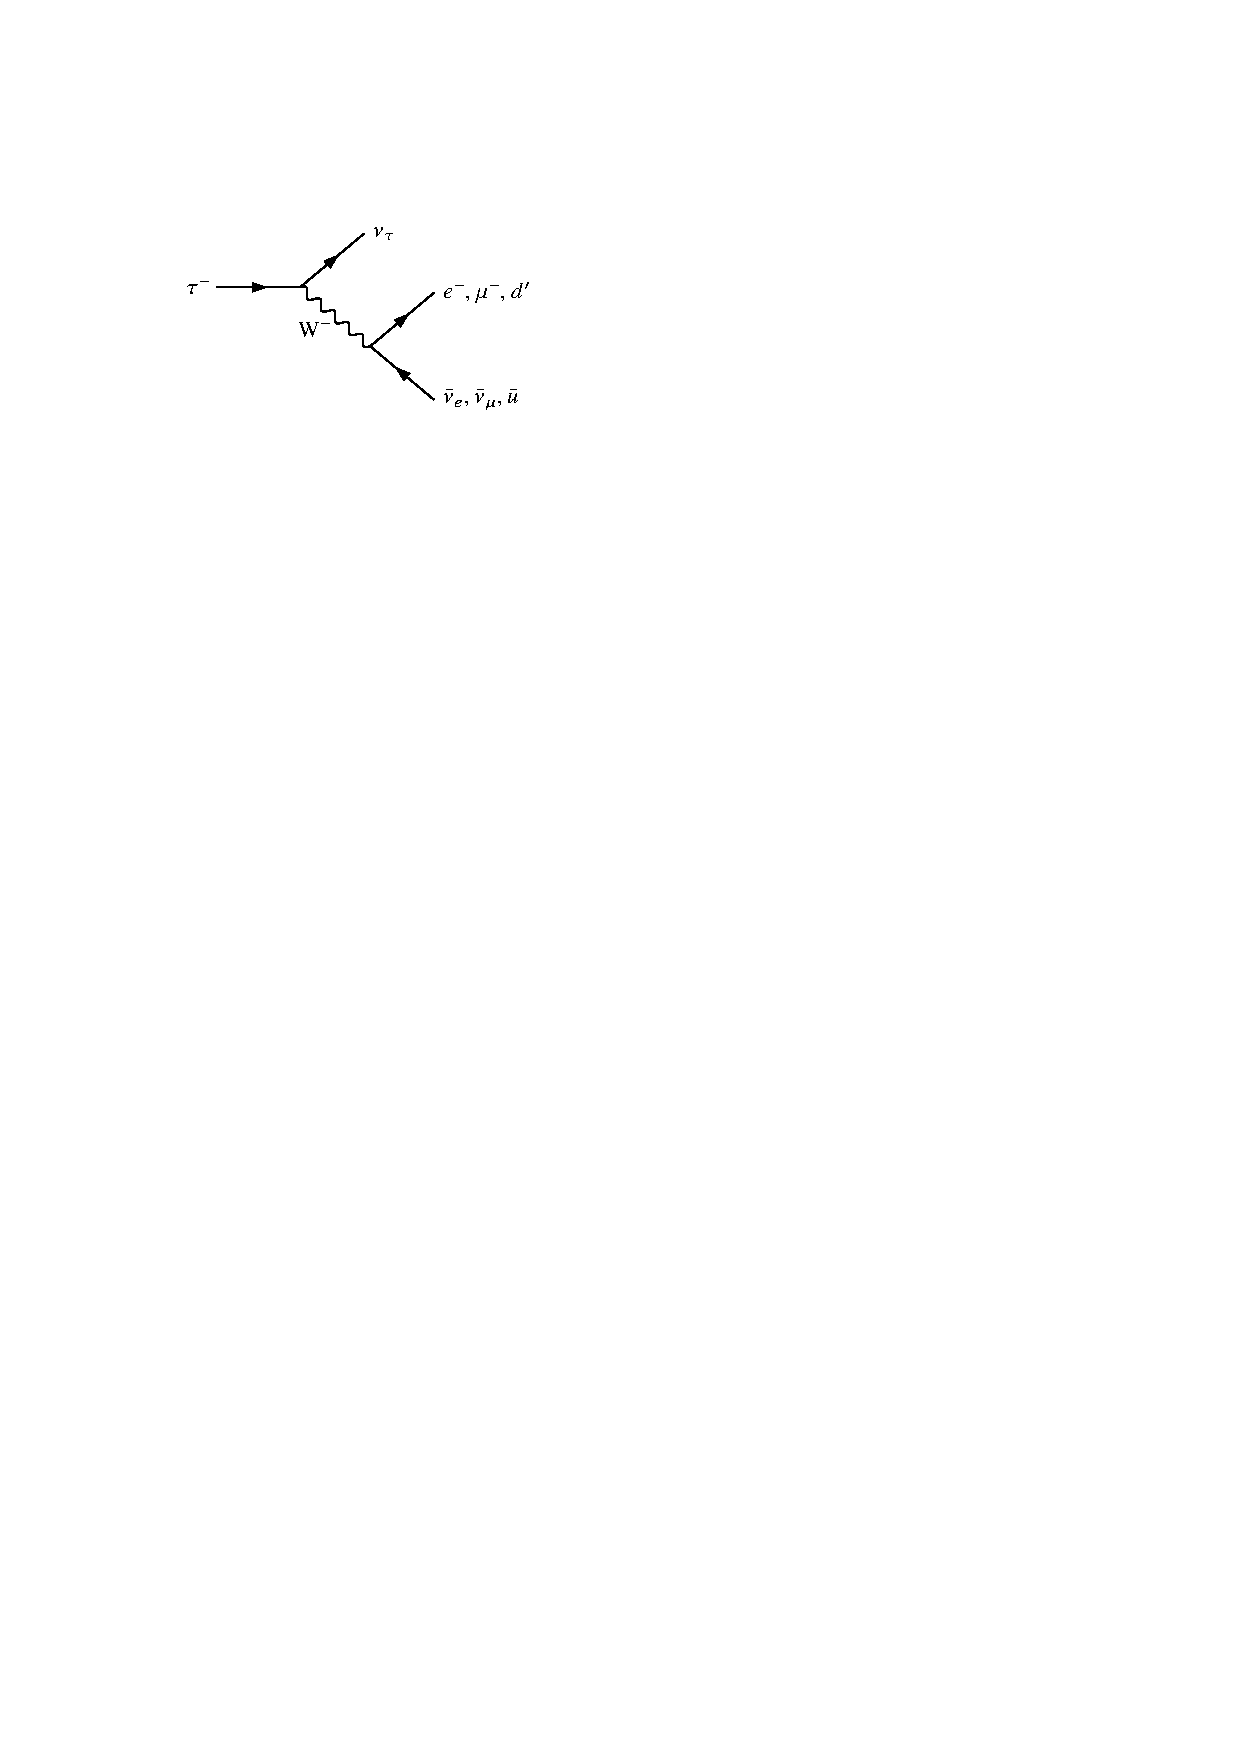
\includegraphics{figs/tauid/tau_decay_feynman}

    \vspace*{3em}
    \subcaption{}%
    \label{fig:tau_feynman}
  \end{subfigure}\hfill
  \begin{subfigure}[b]{0.47\textwidth}
    \centering

    \begin{overpic}[scale=0.9]{figs/tauid/tau_branching_pie_chart}
      \put (31, 83) {$\pi^- \nu_\tau$}
      \put (-5.5, 45) {$\pi^- \pi^0 \nu_\tau$}
      \put (16, 7) {$\pi^- 2 \pi^0 \nu_\tau$}
      \put (40.5, 2) {$2 \pi^- \pi^+ \nu_\tau$}
      \put (65, 6.5) {$2 \pi^- \pi^+ \pi^0 \nu_\tau$}
      \put (76.5, 15.5) {other}
      \put (70, 77.5) {$e^- \bar{\nu}_e \nu_\tau$}
      \put (88.5, 41.5) {$\mu^- \bar{\nu}_\mu \nu_\tau$}
    \end{overpic}

    \subcaption{}%
    \label{fig:tau_branching_ratios}
  \end{subfigure}
  \caption{Decay and branching ratios of the tau
    lepton. Charge-conjugate decay modes are omitted.}
\end{figure}

At the ATLAS experiment, \tauleptons are reconstructed from the signature of
their visible decay products, neglecting any neutrinos produced in the
decay. Leptonic \taulepton decays are reconstructed as electrons or muons using
the reconstruction techniques previously introduced
in~\Cref{sec:ele_rec,sec:muon_rec}. The remainder of this section focuses on the
reconstruction of the visible decay products of hadronic \taulepton decays,
referred to as \tauhadvis, for which dedicated reconstruction techniques are
employed. The reconstruction of \tauhadvis at the beginning of Run~2 is
described in Ref.~\cite{ATLAS-CONF-2017-029}. Several improvements have been
made since, for example the introduction of a multivariate track selection
method~\cite{duschinger}, which are included in the following description.

% Should say something about the signature of a tau jet here
The reconstruction of \tauhadvis is seeded by jets reconstructed using the
anti-\kt algorithm with $R = 0.4$ applied to topo-clusters at LC scale. Only
jets with $\pT > \SI{10}{\GeV}$ and within $|\eta| < 2.5$ are considered as
seeds for \tauhadvis reconstruction.

A PV is associated to the \tauhadvis candidate using information from the
tracking system. The PV association considers ID tracks that are matched to the
seed jet via ghost-association~\cite{Cacciari:2008gn}, are within
$\Delta R < 0.2$ of the jet axis, and fulfil $\pT > \SI{1}{\GeV}$ and basic
track quality criteria. For every PV, the scalar sum of \pT of tracks that are
assigned to the vertex and pass the selection criteria is determined. The PV
maximising this sum is associated to the \tauhadvis candidate and referred to as
the \emph{tau vertex}.

An initial estimate of the \tauhadvis candidate four-momentum is derived by
summing the four-momenta of topo-clusters (at LC scale) in a cone of
$\Delta R < 0.2$ about the jet axis. Moreover, the four-momentum is transformed
into the coordinate system with the tau vertex at its origin. The axis defined
by the tau vertex and the three-momentum of the \tauhadvis candidate is referred
to as the \tauhadvis axis.

Tracks in the ID are associated to a \tauhadvis candidate if they are within
$\Delta R < 0.4$ of the \tauhadvis axis. Tracks originating from charged hadrons
produced in the \taulepton decay are identified by Boosted Decision
Trees~\cite{duschinger}. These tracks are referred to as \emph{core} tracks,
since they are usually found in the \emph{core region} of $\Delta R < 0.2$ about
the \tauhadvis axis. The number of \emph{core} tracks associated to a \tauhadvis
candidate is referred to as \Ntracks. Only candidates with $\Ntracks = 1$ and
$\Ntracks = 3$ are considered and referred to as 1- and 3-prong \tauhadvis
candidates, respectively.\todo{Add a plot showing the improvements?} Tracks not
classified as \emph{core} are classified as \emph{isolation} tracks if they
fulfil
\begin{align*}
  & \pT > \SI{1}{\GeV} && |d_{0}| < \SI{1.0}{\milli\metre} && |z_{0} \sin\theta| < \SI{1.5}{\milli\metre} \\
  & N_{\text{pixel}} \geq 2 && N_{\text{pixel}} + N_{\text{SCT}} \geq 7 \,\text{,}
\end{align*}
where the track parameters are given at the perigee with respect to the tau
vertex. The number of hits on the reconstructed track in the pixel and SCT
detector layers, counting defective sensors located on the trajectory as hits,
is given by $N_{\text{pixel}}$ and $N_{\text{SCT}}$,
respectively. \emph{Isolation} tracks are used to define variables sensitive to
the charged-particle activity in the vicinity of the \tauhadvis candidate.

Calibrations of the \tauhadvis candidate four-momentum to the \tauhadvis energy
scale (TES) are derived using simulated events containing hadronic \taulepton
decays. Two different calibation methods are used:
\begin{description}

\item[Calorimeter-based TES] The calorimeter-based TES is derived from the
  initial estimate of the \tauhadvis four-momentum from topo-clusters (LC scale)
  in the core region of the jet seeding the \tauhadvis. First, the expected
  energy contribution of pile-up to the \tauhadvis is subtracted. This
  subtraction is parameterised as a linear function of the number of
  reconstructed PVs in the event and in bins of \tauhadvis $|\eta|$ and
  \Ntracks. Afterwards, the detector response calibration is performed as a
  function of the \tauhadvis energy after pile-up subtraction and in bins of
  \tauhadvis $|\eta|$ and \Ntracks. The \tauhadvis transverse momentum after
  this calibration step is denoted by \pTLC.

\item[BRT-based TES] The BRT-based TES is derived from \tauhadvis energy
  calibrations performed using Boosted Regression Trees (BRT). This calibration
  uses information from \emph{Tau Particle Flow}
  reconstruction~\cite{PERF-2014-06}, which attempts to reconstruct individual
  charged and neutral hadrons produced in the \taulepton decay, as inputs. Tau
  Particle Flow provides an alternative method to reconstruct the \tauhadvis
  four-momentum with improved angular resolution, and improved energy resolution
  for \tauhadvis with transverse energies below approximately
  \SI{100}{\GeV}~\cite{PERF-2014-06}. The BRT also includes variables sensitive
  to the pile-up conditions, the shapes of showers in the calorimeter, and the
  reconstructed \taulepton decay mode. In addition, \pTLC is included as an
  input since the calorimeter-based estimate of \tauhadvis \pT is superior for
  high-\pT \tauhadvis.

\end{description}
Unless otherwise noted, the BRT-based calibration is used for the remainder of
this thesis. After calibration, the relative \tauhadvis \pT resolution ranges
from \SIrange{5}{7}{\percent}~\cite{ATLAS-CONF-2017-029}.

The \tauhadvis reconstruction techniques presented thus far have limited ability
to reject \tauhadvis candidates originating from sources other than hadronic
\taulepton decays. The primary source being quark- or gluon-initiated jets and
electrons that are mis-reconstructed as \tauhadvis candidates. A separate step,
referred to as \tauid, is performed to reject \tauhadvis candidates from these
sources. A detailed description of \tauid is given in \Cref{sec:tauid}.


\subsection{Missing Transverse Energy}%
\label{sec:atlas_met}





%%% Local Variables:
%%% mode: latex
%%% TeX-master: "../../phd_thesis"
%%% End:



% ==============================================================================
\chapter{Statistical Methods}%
\label{sec:experimental_methods}
%\label{sec:statistical_methods}
% ==============================================================================
% % ==============================================================================
\section{Trigger}
\label{sec:trigger}
% ==============================================================================
\todo[inline]{This should be elsewhere.}

\todo[inline]{For more information on 2017 and 2018 triggers see the
  TauCP INT note.}

The L1 tau trigger (calorimeter only) remained unchanged during Run~2
(aside from topological requirements).

Taxonomy of trigger chains (in athena: HLT threshold, selection, preselection):

\vspace{1em}

\verb|HLT_tau25_medium1_tracktwo| (2015 -- 2016)~\cite{ATLAS-CONF-2017-061}:\\
Three step process:
\begin{enumerate}
\item Calorimeter preselection: The calorimeter is read out in full
  granularity for the region of interest marked by the L1
  trigger. Topoclusters are built from calorimeter cells and
  calibrated with the local hadronic calibration (LC). The vectorial
  sum of clusters defines the jet seed for tau reconstruction. The
  core clusters of the jet seed are used to estimate the tau energy
  which is then calibrated using parametrised methods (subtracting
  pileup and correcting the response). The HLT tau \pT cuts are
  applied at this stage. \verb|tau25|

\item Track preselection (two-staged): Fast tracking (Fast Track
  Finder) is performed in a narrow cone around the center tau jet seed
  to find the highest momentum track to determine the $z$-location of
  the primary vertex from which the tau likely originated. Once the
  vertex is determined, fast tracking is performed over the full ROI
  but restricted in $|\Delta z|$ to be close to the leading
  track. Tracks with at least 1 GeV are kept as core tracks
  $\Delta R < 0.2$ and isolation tracks~$0.2 < \Delta R <
  0.4$. Multiplicity requirements are enforced, so 1 to 3 core tracks
  and maximum 1 isolation track. \verb|tracktwo|

\item Offline-like selection: Precision tracking (similar to offline
  reconstruction) is performed which is seeded using FTF tracks from
  the previous step (i.e. it is refining the tracks found by FTF).


  A BDT (two one for
  1-prong one for multi-prong) is used to identify taus similar to
  what would be used for offline identification of taus. A medium
  working point is chosen with efficiencies: 96\% for 1-prong and 82\%
  for 3-prong in Ztautau. \verb|medium1|
\end{enumerate}

For 2017 data-taking the triggers were similar to the 15--16
algorithms with some tunings of the track preselection to prevent
pile-up from impacting the multiplicity requirements (mostly due to
the upper bound of 3 core tracks for 3-prong taus). Moreover, the
track multiplicity and identification cuts were relaxed for very high
momenta (200 GeV and higher) but this is barely relevant for the work
presented in this thesis.

\vspace{1em}

\verb|HLT_tau25_medium1_tracktwoEF| (2018 -- ):\\
The track multiplicity (core and iso.) which was applied in the track
preselection stage using Fast-Track-Finder tracks introduced
introduced inefficiencies for 3-prong taus in high pileup
conditions. Therefore, the track multiplicity selection was removed
and applied at a later stage on precision tracks that have better
pileup and fake track rejection. \verb|tracktwoEF|

\vspace{1em}

\verb|HLT_tau25_mediumRNN_tracktwoMVA| (2018 K --):\\
The (parametric) calibration in the first step is replaced by an
MVA-based energy calibration using Boosted Regression Trees similar to
the algorithm for offline tau calibration but without track und tau
substructure information. Additionally, the tau identification step is
replaced using the RNN algorithm (similar to offline) with minor
adjustments of input variables (dead sensors in hit counts). Separate
networks are trained for 0-prong and 1-prong.  The multi-prong network
is using the offline tune.  A dedicated medium working point for the
HLT is used with the following efficiency targets: 0-prong: 65\%;
96.5\% 1-prong; 86.5\% multi-prong. The recovery 0-track taus recovers
efficiency for cases (predominantely low momentum / high pileup),
which can happen due to inefficiencies in FTF that are used to seed
precision tracking. These can be recovered in offline reconstruction
with full tracking.


%%% Local Variables:
%%% mode: latex
%%% TeX-master: "../../phd_thesis"
%%% End:

This chapter provides an overview of the statistical methods employed in this
thesis. \Cref{sec:statistical_inference} introduces methods of statistical
inference that are used for the interpretation of the results of
\Cref{sec:dihiggs,sec:higgs_self_coupling}. The machine learning algorithms
employed in \Cref{sec:tauid,sec:dihiggs,sec:higgs_self_coupling} are described
in \Cref{sec:machine_learning}.

%%% Local Variables:
%%% mode: latex
%%% TeX-master: "../../phd_thesis"
%%% End:

% ==============================================================================
\section{Statistical Inference}%
\label{sec:statistical_inference}
% ==============================================================================

This section introduces techniques of statistical inference commonly used in the
ATLAS experiment to interpret the results of searches and measurements. Among
these are methods for parameter estimation, interval estimation, and statistical
hypothesis testing. These are used to fit statistical models to observed data
and to evaluate whether the data indicate the presence of a signal. In this
thesis, statistical software based on \texttt{HistFactory}~\cite{cranmer2012},
\texttt{RooFit}~\cite{Verkerke:2003ir}, and
\texttt{RooStats}~\cite{Moneta:2010pm} is employed for the interpretation of the
results. The following discussion is restricted to statistical models of count
data in a set of disjoint bins. The notation of Ref.~\cite{cranmer2012} is
adopted with few modifications.

% Particle physics workhorse of statistical interpretation:

% - Method of maximum likelihood for point estimation

% - Likelihood ratio tests (or closely related to the Likelihood ratio test) for
% hypothesis testing, estimation of confidence intervals (or limit)

% - Restrict to performing statistical interpretations using binned distributions.

\subsection{The HistFactory Model}

In high-energy physics, the use of binned data is widespread for visualisation
and statistical modelling. Analyses of collider data typically consider multiple
mutually disjoint regions, also referred to as \emph{channels}, defined by
certain event selections. Each region consists of one or more bins defined by a
discriminating variable.

\todo[inline]{Maybe say something about signals / backgrounds and define what a
  'physics process' is? Often count events in bins...}

Let $\mathcal{C}$ denote the set of channels and $\mathcal{B}_{c}$ the set of
bins in channel~$c$. The probability of observing $n_{cb}$ events in bin~$b$ of
channel~$c$ is modelled by a Poisson distribution with probability mass function
$\pois(n_{cb} \vert \nu_{cb})$, where $\nu_{cb}$ denotes the (unknown) expected
number of events for the given bin. The expectation $\nu_{cb}$, which has to be
inferred from the observed data, is parameterised as
\begin{align*}
  \nu_{cb}(\myvec{\alpha}, \myvec{\phi}, \myvec{\gamma}) =
  \sum_{s \in \mathcal{S}_{c}} \, \gamma_{csb} \, \Phi_{cs}(\myvec{\phi}) \, \eta_{cs}(\myvec{\alpha}) \, \sigma_{csb}(\myvec{\alpha}) \,\text{,}
\end{align*}
where $\mathcal{S}_{c}$ is the set of physics processes contributing to
channel~$c$, and $\myvec{\alpha} = (\alpha_1, \dots, \alpha_n)$,
$\myvec{\phi} = (\phi_1, \dots, \phi_m)$, and $\myvec{\gamma}$, which denotes a
vector of all $\gamma_{csb}$, are parameters of the model~\cite{cranmer2012}.
% $\myvec{\alpha} = (\alpha_p)_{p = 1}^{n}$,
% $\myvec{\phi} = (\phi_p)_{p = 1}^m$, $\myvec{\gamma} = (\gamma_{csb})$ are
% parameters, and $\mathcal{S}$ is the set of physics processes that are
% included in the model~\cite{cranmer2012}.
The parameters $\myvec{\alpha}$ and $\myvec{\gamma}$ are nuisance parameters
(NPs) with external constraints, which will be introduced shortly. The relevance
of the four factors $\gamma_{csb}$, $\Phi_{cs}$, $\eta_{cs}$, and $\sigma_{csb}$
is described in the following~\cite{cranmer2012}:
\begin{itemize}

\item $\sigma_{csb}(\myvec{\alpha})$ is referred to as the \emph{parameterised
    histogram} of process~$s$ in channel~$c$, the index $b$ denoting the bins of
  the histogram. It serves to estimate the expected number of events from
  process~$s$ in channel~$c$ and is usually derived using simulation or control
  region data. The parameterised histogram has additional degrees of freedom,
  parameterised by $\myvec{\alpha}$, to account for uncertainties on the shape
  of the histogram. These degrees of freedom leave the overall normalisation
  $\sum_{b \in \mathcal{B}_{c}} \sigma_{csb}(\myvec{\alpha})$ for a given
  channel~$c$ and process~$s$ unchanged.

\item $\eta_{cs}(\myvec{\alpha})$ represents a normalisation factor applied
  uniformly to all bins of the parameterised histogram for a given process~$s$
  in channel~$c$. The normalisation factor $\eta_{cs}$ cannot vary freely since
  it is a function of the constrained NPs~$\myvec{\alpha}$. This factor is
  included to account for uncertainties on the normalisation of process~$s$ in
  channel~$c$.

\item $\Phi_{cs}(\myvec{\phi})$ also represents a normalisation factor applied
  uniformly to all bins of the parameterised histogram for a given process~$s$
  in channel~$c$. However, $\Phi_{cs}$ is the product of \emph{free}
  (unconstrained) normalisation factors given by
  \begin{align*}
    \Phi_{cs}(\myvec{\phi}) = \prod_{p \in \mathcal{N}_{cs}} \phi_p \,\text{,}
  \end{align*}
  where $\mathcal{N}_{cs}$ denotes the set of indices that defines which free
  normalisation factors are to be applied to a given process~$s$ in channel~$c$.
  % These parameters are optional, i.e.\ they can be fixed to unity for a given
  % process/channel depending on the statistical model one wants to construct.
  % % Normalisation factors that are shared?
  In most cases, at least one normalisation factor is present that is applied to
  the physics process of interest, also referred to as the \emph{signal}. This
  normalisation factor is referred to as the \emph{signal strength}, $\mu$, and
  is often considered to be the parameter of interest (POI). Normalisation
  factors are considered to be NPs if they are not POIs.

\item $\gamma_{csb}$ are parameters that introduce additional degrees of freedom
  for every channel, process, and bin. They are used to incorporate
  uncertainties that originate from sources that are independent between
  channels, processes, and bins. An example of such an uncertainty is the
  statistical uncertainty arising from the use of finite samples of events to
  estimate $\sigma_{csb}$.

  In this thesis, the method by Barlow and Beeston~\cite{barlow1993} is used to
  account for statistical uncertainties on $\sigma_{csb}$. To reduce the number
  of parameters of the statistical model, the method is simplified as proposed
  in Ref.~\cite{conway2011} by only considering the statistical uncertainty on
  $\sum_{s \in \mathcal{S}} \sigma_{csb}$ for a given bin and
  channel. Consequently, the parameters $\gamma_{csb}$ can be replaced by
  $\gamma_{cb}$, omitting the dependence on the physics process.

\end{itemize}
A description of the exact functional form of $\sigma_{csb}(\myvec{\alpha})$ and
$\eta_{cs}(\myvec{\alpha})$ is omitted here but can be found in
Ref.~\cite{cranmer2012}. The likelihood function of the statistical model is
given by
\begin{align}
  L(\myvec{\alpha}, \myvec{\phi}, \myvec{\gamma}) = \Biggl[\,
  \prod_{c \in \mathcal{C}}
  \prod_{b \in \mathcal{B}_{c}}
  \pois\bigl( n_{cb} \big| \nu_{cb}(\myvec{\alpha}, \myvec{\phi}, \myvec{\gamma}) \bigr)
  \,\Biggr]
  \times L_{\text{ext}}(\myvec{\alpha}, \myvec{\gamma}) \,\text{,}
  \label{eq:likelihood_histfactory}
\end{align}
where $L_{\text{ext}}(\myvec{\alpha}, \myvec{\gamma})$ is the likelihood
function defining the external constraints on the NPs~$\myvec{\alpha}$ and
$\myvec{\gamma}$. The external constraints are defined by
\begin{align*}
  L_{\text{ext}}(\myvec{\alpha}, \myvec{\gamma}) =
  \Biggl[\, \prod_{p=1}^{n} f(a_p \vert \alpha_p)     \,\Biggr]
  \Biggl[\, \prod_{c \in \mathcal{C}} \prod_{b \in \mathcal{B}_{c}} \pois(m_{cb} \vert \gamma_{cb} \tau_{cb}) \,\Biggr] \,\text{,}
\end{align*}
the two terms in brackets are elaborated hereafter:
\begin{itemize}

\item

  The first term describes the constraints

  $a = 0$ such that the MLE of $\hat{\alpha} = 0$

  $f(a \vert \alpha)$ denotes the probability density of a Normal distribution
  with unit variance and mean of $\alpha$.

  In isolation, this term describes an auxiliary measurement yielding a
  $\alpha_p$ confidence interval of $[-1, 1]$ at \SI{68}{\percent} confidence
  level. Therefore, the

  \SI{68}{\percent} confidence interval is given by $\alpha_p \in [-1, 1]$,
  hence $\alpha_p = \pm 1$ is interpreted as $\pm 1 \sigma$

\item

\end{itemize}


where the first bracket defines the constraints on
$\myvec{\alpha} = (\alpha_p)_p$ and the second one



The statistical model of
the auxiliary measurements constraining the NPs $\myvec{\alpha}$ is constructed
from





In this thesis, $f_p(a_p \vert \alpha_p)$ denotes the probability density of a
Normal distribution with mean~$\alpha_p$ and unit variance.




The statistical model of the auxiliary measurements constraining the NPs
$\myvec{\alpha}$ is closely connected to the functional form of
$\sigma_{csb}(\myvec{\alpha})$ and $\eta_{cs}(\myvec{\alpha})$, thus only a
general introduction is given.



These measurements are usually defined by performing comparisons of


with alternative predictions that characterise systematic uncertainties


Often, these
measurements are defined by a comparison


The likelihood function of the auxiliary measurement is given by

\vspace{5em}

The parameters of the model can be estimated, given the observed data, using
maximum likelihood estimation. Hereafter, it is assumed that the model has one
POI denoted by $\mu$ that is to be interpreted as a signal strength. All other
(non-POI) parameters of the model are collectively referred to as
$\myvec{\theta}$. Let $\Omega$ be the parameter space of the model with
elements~$(\mu, \myvec{\theta})$. The maximum likelihood estimate (MLE) of the
parameters are determined by the \emph{unconditional fit}
\begin{align}
  (\muhat, \hat{\myvec{\theta}}) = \argmax_{(\mu, \myvec{\theta}) \in \Omega} L(\mu, \myvec{\theta}) \,\text{.}
  \label{eq:unconditional_fit}
\end{align}
Often, a restricted model is constructed by fixing the POI to an arbitrary value
$\mu^*$. In this case, the MLE of the model parameters are given by the
\emph{conditional fit for $\mu = \mu^*$}
\begin{align}
  \hat{\hat{\myvec{\theta}}}(\mu^*) = \argmax_{\myvec{\theta} \in \{ \myvec{\theta}^\prime \mid (\mu^\prime, \myvec{\theta}^\prime) \in \Omega \,\land\, \mu^\prime = \mu^* \} } L(\mu^*, \myvec{\theta}) \,\text{.}
  \label{eq:conditional_fit}
\end{align}
Hereafter, the model with the restriction $\mu = 0$ is referred to as the
\emph{background-only model}. The unrestricted model is referred to as the
\emph{signal-plus-background model}.

\todo[inline]{Asimov dataset.}

Lastly,

Asimov datasets -> all observables are set to their expected values.

expected experimental sensitivity prior to looking at the recorded data.

referred to as a \emph{Asimov dataset}

An Asimov dataset can be used in place of data to determine the expected
experimental sensitivity.


\subsection{Hypothesis Testing}

In high-energy physics, one is often concerned with comparing the goodness of
fit of competing statistical models to observed data. These comparisons allow to
make statements about values of the signal strength that are still in agreement
with the observations. The framework of \emph{statistical hypothesis testing}
provides a principled approach to perform these comparisons.

With the statistical model introduced previously, the null hypothesis, $H_0$, is
given by
\begin{align*}
  H_0: (\mu, \myvec{\theta}) \in \Omega_0
  \quad \text{with} \quad \Omega_0 \subset \Omega \,\text{,}
\end{align*}
where $\Omega_0$ is the set of model parameters defining the null
hypothesis,\footnote{Example: Taking the background-only hypothesis as the null
  hypothesis, then
  $\Omega_0 = \{ (\mu^\prime, \myvec{\theta}^\prime) \in \Omega \mid \mu^\prime
  = 0 \}$.}  and the alternative hypothesis, $H_1$, by
\begin{align*}
  H_1: (\mu, \myvec{\theta}) \in \Omega_1
  \quad \text{with} \quad \Omega_1 = \Omega \setminus \Omega_0 \,\text{.}
\end{align*}
A \emph{likelihood ratio test} (LRT) can be used to compare both hypotheses. The
test statistic of the LRT is given by
\begin{align*}
  \Lambda = -2 \ln \left[
  \frac{\sup_{(\mu, \myvec{\theta}) \in \Omega_0} L(\mu, \myvec{\theta})}
  {\sup_{(\mu, \myvec{\theta}) \in \Omega\phantom{_0}} L(\mu, \myvec{\theta})}
  \right] \,\text{,}
\end{align*}
where the numerator (denominator) of the term in brackets is the supremum of the
likelihood for the restricted (unrestricted) model~\cite{casella2001}. A
critical value of the test statistic, $\Lambda_{\text{crit}}$, is chosen and
compared to the observed value of the test statistic. If
$\Lambda > \Lambda_{\text{crit}}$ then $H_0$ is rejected in favour of
$H_1$. Otherwise, $H_0$ cannot be rejected. The chosen value of
$\Lambda_{\text{crit}}$ defines the rejection region of the test and thus its
statistical significance and power.


\subsubsection{Discovery of a Signal}

In the framework of hypothesis testing, the discovery of a signal implies
rejecting the background-only hypothesis in favour of the signal-plus-background
hypothesis. Usually, only signals with positive strength, that is $\mu > 0$, are
considered as potential discoveries. The relevant hypotheses for testing the
discovery of a signal are
\begin{align*}
  &H_0: (\mu, \myvec{\theta}) \in \{ (\mu^\prime, \myvec{\theta}^\prime) \in \Omega^+ \mid \mu^\prime = 0 \}
  &&H_1: (\mu, \myvec{\theta}) \in \{ (\mu^\prime, \myvec{\theta}^\prime) \in \Omega^+ \mid \mu^\prime > 0 \} \,\text{,}
\end{align*}
where $\Omega^+$ denotes the parameter space of the model with the restriction
that $\mu \geq 0$. An empirical test statistic based on the LRT is defined as
\begin{align*}
  q_0 = \begin{cases}
          -2 \ln \left[ \frac{ L\bigl(0, \hat{\hat{\myvec{\theta}}}(0) \bigr)}{L\bigl( \muhat, \hat{\myvec{\theta}} \bigr)} \right], & \muhat > 0 \\
          0,          & \muhat \leq 0
        \end{cases} \quad\text{,}
\end{align*}
where $\muhat$, $\hat{\myvec{\theta}}$, and $\hat{\hat{\myvec{\theta}}}$ are
defined as in
\Cref{eq:unconditional_fit,eq:conditional_fit}~\cite{Cowan:2010js}.\footnote{The
  unconditional fit is performed without the $\mu \geq 0$ constraint. Instead,
  the constraint is imposed in the definition of the test statistic by setting
  the maximum likelihood of the unrestricted model to
  $L\bigl( 0, \hat{\hat{\myvec{\theta}}}(0) \bigr)$ in the $\muhat < 0$ case.}
This test statistic is referred to as the \emph{discovery test statistic}. The
asymptotic sampling distribution of $q_0$ under $H_0$ is given by the
probability density function
\begin{align*}
  f(q_0) = \frac{1}{2} \delta(q_0) + \frac{1}{2} f_{\chi^2}(q_0; 1) \,\text{,}
\end{align*}
which is an equal mixture of a Dirac $\delta$ distribution and a $\chi^2$
distribution with one degree of freedom~\cite{Cowan:2010js}. The discovery test
statistic is often expressed in terms of an asymptotic $p$-value according
to
\begin{align*}
  p_0 = \int_{q_{0}}^\infty \mathrm{d}q_0^\prime \, f(q_0^\prime) =
  1 - \Phi\left(\sqrt{q_{0}}\right) \,\text{,}
\end{align*}
where $\Phi$ is the cumulative distribution function of the Standard Normal
distribution~\cite{Cowan:2010js}. Another way of expressing the test statistic
is in terms of the \emph{discovery significance}~$Z_0$, which is defined
as~\cite{Cowan:2010js}
\begin{align*}
  Z_0 = \Phi^{-1}(1 - p_0) = \sqrt{q_{0}} \,\text{.}
\end{align*}
In particle physics, the conventional significance threshold that has to be
exceeded to claim discovery of new physics is $Z_0 = 5$ ($p_0 = \num{2.87e-7}$),
which is also referred to as the ``$5\sigma$ threshold''.


\subsubsection{Upper Limits on the Signal Strength}

Often, it is of interest to determine the largest signal strength that would
still be compatible with the observed data. Formally, this constitutes
estimating a one-sided confidence interval for $\mu$ that is bounded from above,
hence referred to as an upper limit. The upper limit can be determined by
inverting a test of the hypotheses
\begin{align*}
  &H_0: (\mu, \myvec{\theta}) \in \{ (\mu^\prime, \myvec{\theta}^\prime) \in \Omega^+ \mid \mu^\prime \geq \mu^* \}
  &&H_1: (\mu, \myvec{\theta}) \in \{ (\mu^\prime, \myvec{\theta}^\prime) \in \Omega^+ \mid \mu^\prime < \mu^* \} \,\text{,}
\end{align*}
where $\mu^*$ is a parameter and it is assumed that $\mu$ is non-negative. Let
$(1 - \alpha)$ be the desired confidence level (CL) of the interval to be
estimated. Given a test of $H_0$ and $H_1$ with significance level~$\alpha$, the
confidence interval is given by the values of $\mu^*$ for which $H_0$ cannot be
rejected by the test. The largest value of $\mu^*$ for which this condition
holds is referred to as the upper limit on $\mu$ at $(1-\alpha)$~CL. The
determination of upper limits in HEP uses an empirical test statistic derived
from the LRT that reads
\begin{align*}
  \qmutilde =
  \begin{cases}
    -2\ln\left[ \frac{ L\bigl( \mu, \hat{\hat{\myvec{\theta}}}(\mu) \bigr)}{L\bigl( 0, \hat{\hat{\myvec{\theta}}}(0) \bigr)} \right], & \muhat \in (\infty, 0] \\[1em]
    -2\ln\left[ \frac{ L\bigl( \mu, \hat{\hat{\myvec{\theta}}}(\mu) \bigr)}{L\bigl( \muhat, \hat{\myvec{\theta}} \bigr)} \right], & \muhat \in (0, \mu] \\[1em]
    0,\phantom{ \biggl[  \biggr]} & \muhat \in (\mu, \infty) \\
  \end{cases} \,\text{,}
\end{align*}
where for notational simplicity $\mu^*$ is denoted as
$\mu$~\cite{Cowan:2010js}. The asymptotic sampling distributions of \qmutilde
were derived in Ref.~\cite{Cowan:2010js} for any assumed value of the signal
strength. Let~$f(\qmutilde \mid \mu^\prime)$ be the asymptotic sampling
distribution of \qmutilde under the assumption that the signal strength is
$\mu^\prime$.







\begin{align*}
  p_\mu = \int_{\tilde{q}_{\mu, \text{obs}}}^{\infty} \mathrm{d}\qmutilde \, f(\qmutilde \mid \mu) \\
  p_{\text{b}} = \int_{0}^{\tilde{q}_{\mu, \text{obs}}} \mathrm{d}\qmutilde \, f(\qmutilde \mid 0)
\end{align*}



until $p_\mu$ is equal to the chosen value of $\alpha$.


However, in particle physics






\vspace{5em}

Conventionally, upper limits are set at $\SI{95}{\percent}$ CL
($\alpha = 0.05$) in HEP. An empirical test statistic derived from the LRT is
defined according to


Conventionally, upper limits are set at $\SI{95}{\percent}$~CL
($\alpha = 0.05$) in HEP, although using a more conservative approach that will
be introduced shortly.


Using the asymptotic approximation, an iterative procedure can be employed to
find the value of $\mu$ such that
\begin{align*}
  \CLsb
  = 1 - \int_{\tilde{q}_{\mu, \text{obs}}}^{\infty} \mathrm{d}\tilde{q}_{\mu} \, f(\tilde{q}_{\mu} \mid \mu)
\end{align*}
is equal to \SI{95}{\percent}.



However, in particle physics a more conservative approach is taken to set upper
limits. The \CLs method


CLs method: \cite{Read:2002hq}

\begin{align}
  \text{CL}_\text{s+b} = \int^\infty_{q_\text{obs}} f(\tilde{q}_\mu \mid \mu) \, \mathrm{d}\tilde{q}_\mu \\
  \text{CL}_\text{b} = \int^\infty_{q_\text{obs}} f(\tilde{q}_\mu \mid 0) \, \mathrm{d}\tilde{q}_\mu
\end{align}


\begin{align}
  \text{CL}_\text{s} = \frac{\text{CL}_\text{s+b}}{\text{CL}_\text{b}}
\end{align}


\subsection{Treatment of Statistical Uncertainties on Background Rate
  Predictions}%
\label{sec:barlow_beeston}

The predicted background rate in a given bin $b$ of a channel $c$ is
determined from a finite sample of events, e.g.\ from MC simulation,
and thus does not directly correspond to the true expected rate. The
background rate estimates are subject to uncertainties that have to be
considered when performing inference, particularly when bins are only
sparsely populated with events.

This uncertainty is included in the likelihood function, employing the
method proposed by Barlow and Beeston~\cite{barlow1993}, by replacing
the expected background rate from the prediction using the finite
sample with the true expected rate that has to be simultaneously
inferred. In practice this is done by performing the substitution
$\nu_{cb} \rightarrow \gamma_{cb} \nu_{cb}$ that introduces new
nuisance parameters $\gamma_{cb}$ specifying the relative difference
between the predicted and true expected rates. Initially it was
proposed to introduce one such nuisance parameter for every background
source~\cite{barlow1993}, however, a simplified version proposed in
Ref.~\cite{conway2011} is used such that only the combined uncertainty
on the total background prediction is considered instead.

The $\gamma$ nuisance parameters are constrained by auxiliary
measurements using the observed samples of events entering the
bins. These measurements contribute terms of the form
\begin{align*}
  \pois(m_{cb} | \gamma_{cb} \tau_{cb})
  \qquad \text{with} \qquad
  \tau_{cb} = \frac{( \sum_i w_i )^2}{\sum_i w_i^2} = \text{const.}
\end{align*}
to the likelihood function~\cite{cranmer2012}, where the sums go over
all events contributing to bin $b$ in channel $c$ with event weights
$w_i$. This corresponds to a measurement of the effective number of
events based on the observed value $m_{cb}$, which is nominally equal
to $\tau_{cb}$\footnote{It should be noted that $m_{cb}$ are generally
  not integer-valued quantities and thus do not agree with the support
  of the Poisson distribution. Thus the factorial term in the Poisson
  PMF is replaced by the continuous gamma function to generalise the
  distribution to $\mathbb{R}^+$.}, from the finite sample.

This approach is based on the approximation of the \emph{compound
  Poisson distribution} (CPD) that describes the distribution of the
sum of a Poisson number of random weights with a \emph{scaled Poisson
  distribution} (SPD)~\cite{Bohm:2013gla}. The CPD describes the
distribution of rate predictions based on a finite sample of weighted
events and can be defined as
\begin{align*}
  X = \sum_{i = 1}^{N} W_i \quad \text{with} \quad N \sim \pois(\lambda) \quad \text{and} \quad \text{i.i.d.\ } W_i \text{ (independent of }N\text{)} \,\text{.}
\end{align*}
It can be approximated, see for example Ref.~\cite{Bohm:2013gla},
using a scaled Poisson distribution defined by
\begin{align*}
  \tilde{X} = s \cdot \tilde{N} \quad \text{with} \quad \tilde{N} \sim \pois(\tilde{\lambda})
\end{align*}
with
\begin{align*}
  s = \frac{\expect(W^2)}{\expect(W)} \qquad \tilde{\lambda} = \frac{\lambda \expect(W)^2}{\expect(W^2)}
\end{align*}
where $\expect(W)$ and $\expect(W^2)$ are the first and second moment
of the weight distribution. The Barlow-Beeston method makes the
assumption that the expectation values can be approximated by sample
averages such that
\begin{align*}
  s = \frac{\sum_i w_i^2}{\sum_i w_i} \qquad \tilde{\lambda} = \frac{\lambda}{n} \frac{(\sum_i w_i)^2}{\sum_i w_i^2}
\end{align*}
with sample size $n$. Comparing the equation for $\tilde{\lambda}$
with the constraint term entering the likelihood function illustrates
the connection to a measurement of the effective number of events. A
number of $\tilde{N}$ events contribute with equal weights given by
$s$ to the sum, thus $\tilde{N}$ can be referred to as an effective
number of events.

These relationships will be needed in the context of the statistical
interpretation of the results in~\Cref{sec:toys_global_observables}.


%%% Local Variables:
%%% mode: latex
%%% TeX-master: "../../phd_thesis"
%%% End:

\section{Machine Learning}

\begin{itemize}
\item What is machine learning?

\item Why is it useful for HEP? (Problems are multivariate... -- with high-order
  interactions between variables)

\item Supervised learning, i.e.\ have labelled data.

\item Binary classification tasks: Every training example has a label indicating
  the class membership. -> Focus on classification tasks

\item In HEP, the positive class is typically referred to as \emph{signal} while
  the negative class is referred to as \emph{background}.

\item What is training data, etc.

\item What is training.

\item Overfitting?
\end{itemize}


\subsection{Boosted Decision Trees}

Boosted decision trees (BDT) are classification and regression algorithms
composed of multiple \emph{decision trees}. This ensemble of decision trees is
created using an algorithm referred to as \emph{boosting}, which iteratively
fits shallow decision trees--or in general, any \emph{weak learning
  algorithm}--to altered versions of the training data. The training data is
modified at every iteration to emphasise errors made in previous
iterations. Finally, the predictions of the ensemble of trees are combined with
the goal of providing superior classification/regression performance compared to
a single decision tree. In the following a description of one of the BDT
algorithms implemented in \textsc{TMVA}~\cite{TMVA} is given, which is later
used in the search for Higgs boson pair production.


\subsubsection{Classification and Regression Trees}

Classification and regression trees~\cite{Breiman:1984jka,hastie09}, hereafter
collectively referred to as \emph{decision trees}, are used as the basis for
BDT. A decision tree partitions an $n$-dimensional space with coordinates
$\myvec{x} = (x_1, \dots, x_n)$ by recursively performing binary splits along
the coordinate axes until a stopping criterion is met. The resulting binary tree
structure and partitioning is illustrated in \Cref{fig:decision_tree} for a
two-dimensional example. A decision tree with $J$~leaf nodes partitions the
input space into $J$~mutually disjoint subregions denoted by $R_j$ for
$j = 1, \dots, J$. A constant value $c_j$ is assigned to every region $R_j$ such
that the prediction of a decision tree for a point~$\myvec{x}$ can expressed as
\begin{align*}
  h\bigl( \myvec{x}; \{c_j, R_j\}_{j=1}^{J} \bigr) = \sum_{j = 1}^{J} c_j \, \mathbf{1}(\myvec{x} \in R_j) \qquad \text{with} \qquad \mathbf{1}(\myvec{x} \in R_j) =
  \begin{cases}
    1, & \myvec{x} \in R_j \\
    0, & \text{else}
  \end{cases} \,\text{,}
\end{align*}
where $\{c_j, R_j\}_{j=1}^{J}$ fully specifies the decision
tree~\cite{hastie09}.

\begin{figure}[htbp]
  \centering

  \begin{subfigure}[b]{0.46\textwidth}
    \centering
    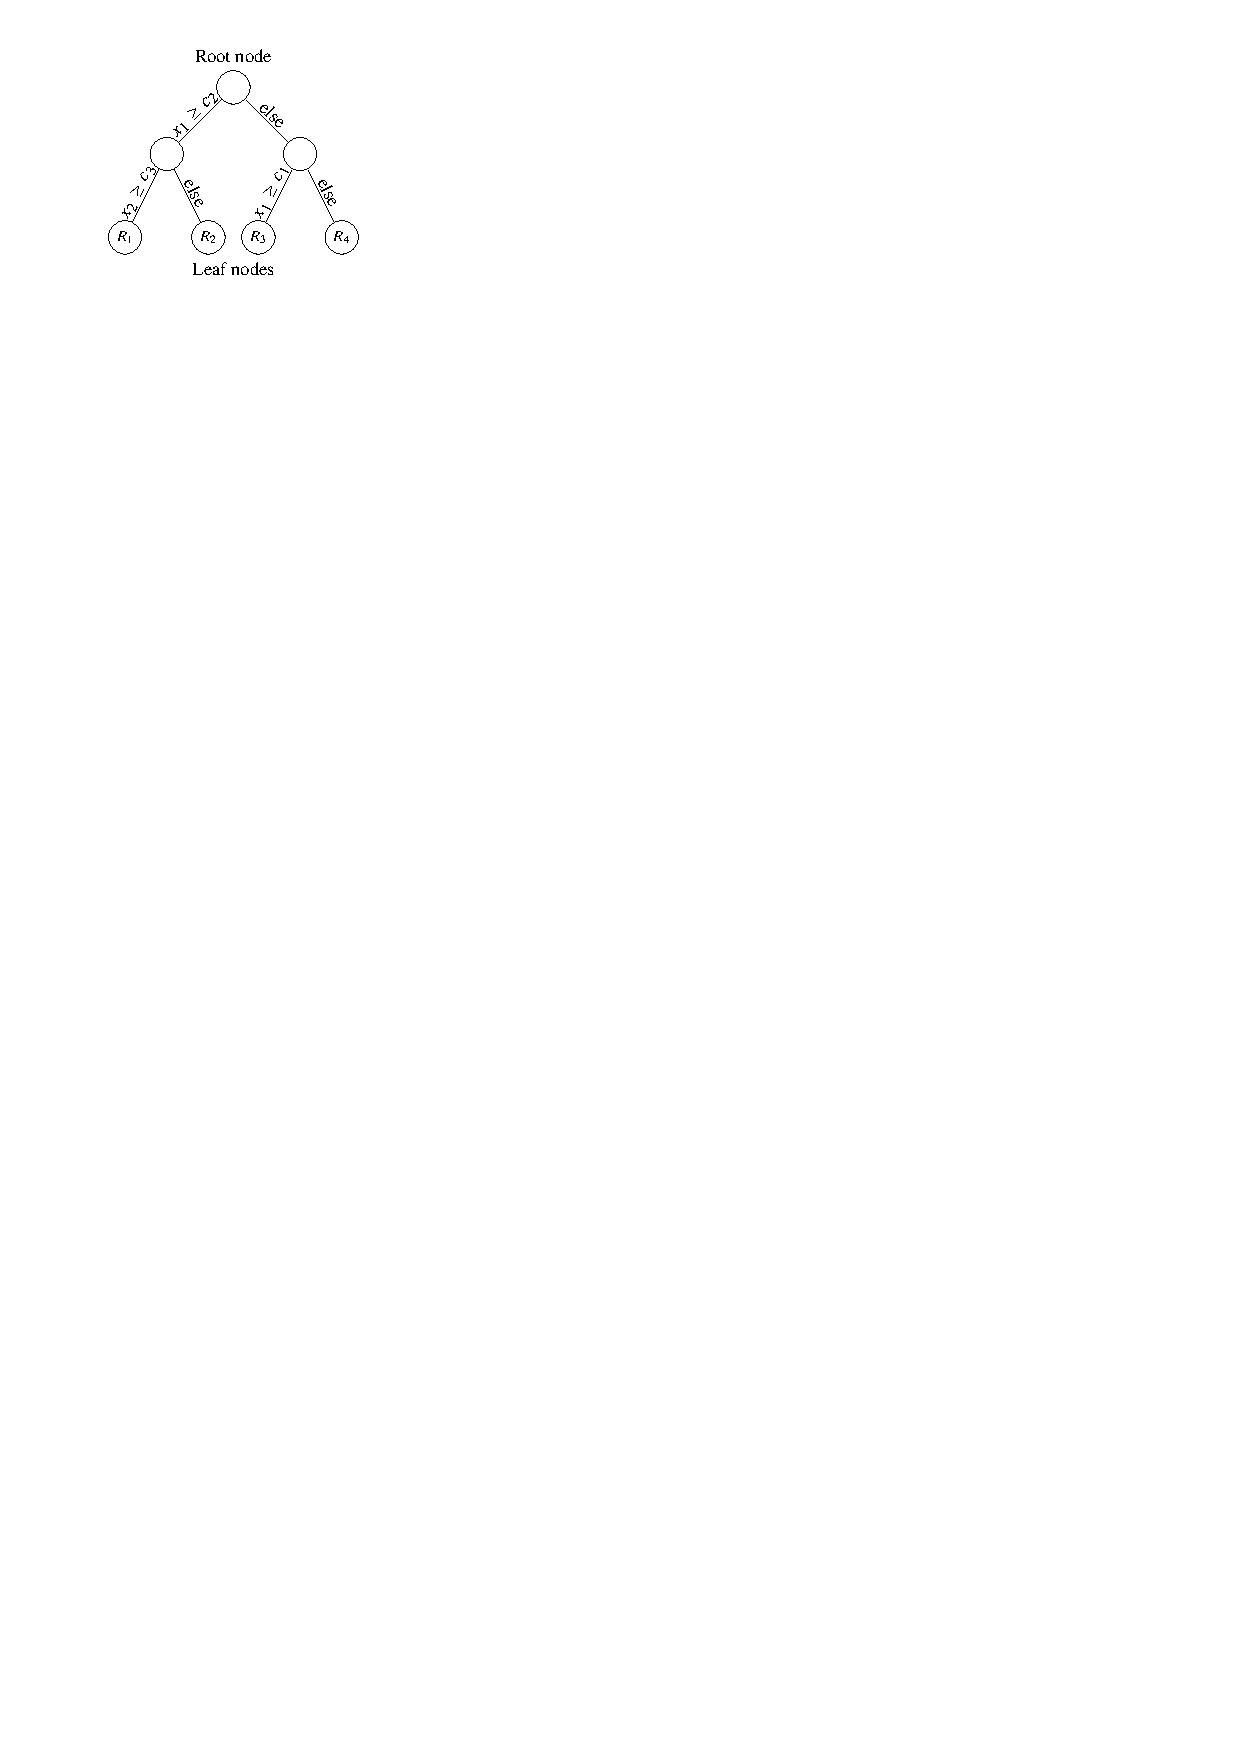
\includegraphics[scale=1.05]{ml/decision_tree}
    \caption{Binary tree structure of a decision tree.}
  \end{subfigure}\hfill%
  \begin{subfigure}[b]{0.46\textwidth}
    \centering
    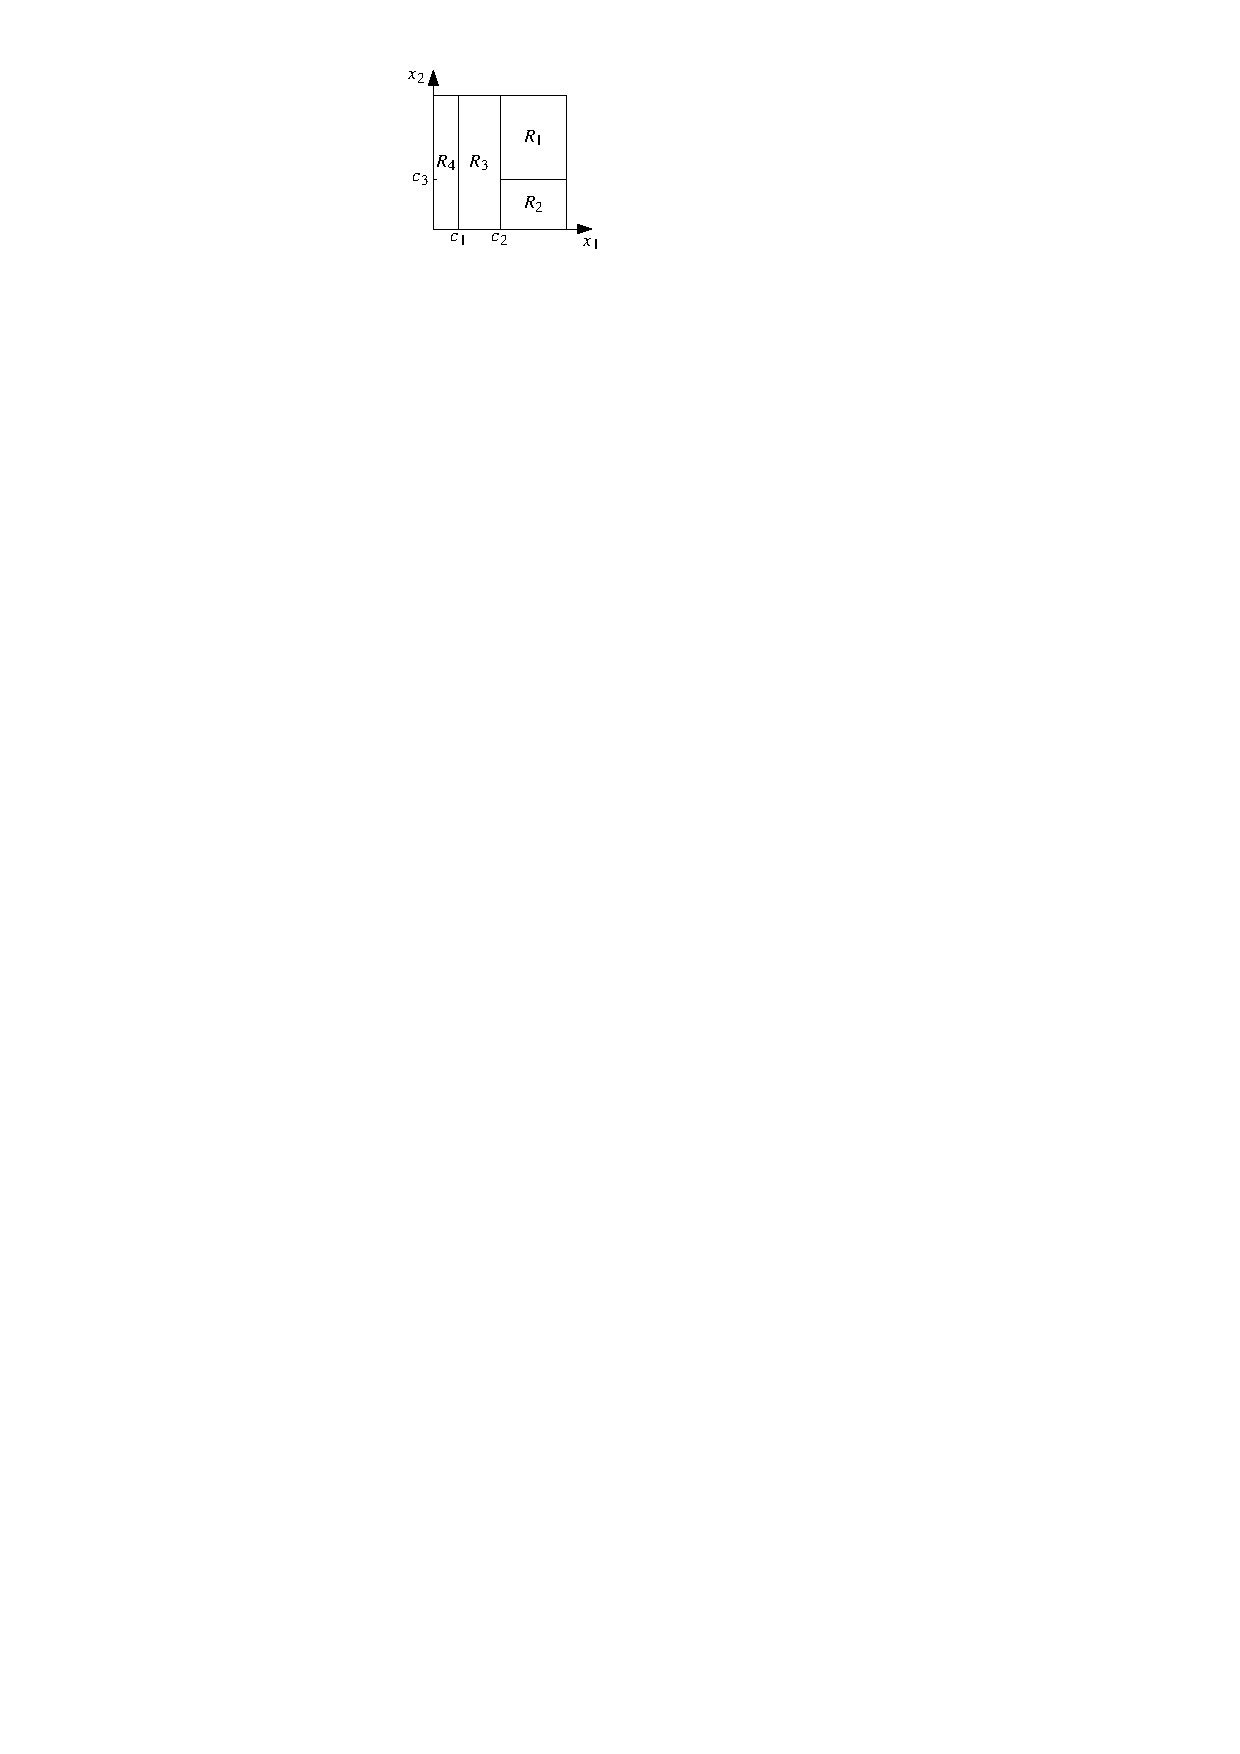
\includegraphics[scale=1.05]{ml/decision_tree_partitioning}
    \vspace*{0.7em}
    \caption{Partitioning resulting from the binary tree in (a).}
  \end{subfigure}\hfill%

  \caption{Example of a decision tree operating on a two-dimensional space with
    coordinates $\myvec{x} = (x_1, x_2)$. The tree has a depth of two and four
    leaf nodes that define the regions $R_1, \dots, R_4$. The figure is adapted
    from Ref.~\cite{hastie09}.}%
  \label{fig:decision_tree}
\end{figure}

Classification trees are constructed with the goal that the partitioning of the
input space yields subregions with low impurity, that is, the regions are mostly
populated by training examples of a single class. In this case, the impurity of
a tree node is quantified by the Gini index
\begin{align*}
  I_{\text{G}}(p) = 2 p (1 - p) \,\text{,}
\end{align*}
where $p$ is the proportion of examples from the positive class in a given
node~\cite{hastie09}. A \emph{greedy} strategy is adopted to grow decision trees
by performing the best possible split at every node. This split is determined by
minimising the weighted sum of Gini impurities of the resulting daughter nodes,
where impurities are weighted according to the total weight of training examples
populating a given node. In the classification case, the constants $c_j$
assigned to leaf nodes of the tree are either--depending on the algorithm
configuration--the proportion of examples from the positive class or the class
label of the majority class in a given leaf node.

Regression trees are constructed using a similar approach, however, with an
altered splitting criterion and different assignment of constants to leaf
nodes. Consider the split of a parent node into a left (L) and right (R)
daughter node. Let $(y, w)$ denote the tuple of regression target and weight of
a given training example. Moreover, let $T_{\text{L}}$ and $T_{\text{R}}$ denote
the set of $(y, w)$ for training examples populating the left and right daughter
node, respectively. The constants $c_{\text{L}}$ and $c_{\text{R}}$ assigned to
the daughter nodes are given by
\begin{align*}
  c_{\text{L}} = \frac{\sum_{(y, w) \in T_{\text{L}}} w y}{\sum_{(y, w) \in T_{\text{L}}} w} \qquad \text{and} \qquad c_{\text{R}} = \frac{\sum_{(y, w) \in T_{\text{R}}} w y}{\sum_{(y, w) \in T_{\text{R}}} w} \,\text{,}
\end{align*}
which is the weighted mean of the regression target for the training examples
populating the left and right node, respectively. The best possible split of a
node in a regression tree is chosen such that the squared error defined as
\begin{align*}
  \sum_{(y, w) \in T_{\text{L}}} w (y - c_{\text{L}})^2 + \sum_{(y, w) \in T_{\text{R}} } w (y - c_{\text{R}})^2
\end{align*}
is minimised.


\subsubsection{Boosting of Decision Trees}

Boosting is an approach of solving predictions tasks by constructing additive
models of the form
\begin{align*}
  F_{M}\bigl(\myvec{x}; \{ \beta_m, \gamma_{m} \}_{m=1}^{M} \bigr) = \sum_{m = 1}^{M} \beta_m b(\myvec{x}; \gamma_{m}) \,\text{,}
\end{align*}
where $\beta_m$ are coefficients and $b(\myvec{x}; \gamma_{m})$ are basis
functions parameterised
by~$\gamma_{m}$~\cite{Friedman:2000,Friedman:2001wbq}. While there is some
flexibility in choosing the family of basis functions, boosting is typically
applied to decision trees.
% Given a sample of training data, the model is fit using an
% iterative procedure in which the $m$-th stage of the model, which is given by
% \begin{align*}
%   F_{m}\bigl(\myvec{x}; \{ \beta_{n}, \gamma_{n} \}_{n=1}^{m} \bigr) = F_{m - 1}\bigl( \myvec{x}; \{ \beta_{n}, \gamma_{n} \}_{n=1}^{m-1} \bigr) + \beta_m b(\myvec{x}; \gamma_{m}) \,\text{,}
% \end{align*}
% is determined by choosing $\beta_{m}$ and $\gamma_{m}$ such that an objective
% function is improved~\cite{hastie09}. Notably, the $m$-th stage does not alter
% the parameters~$\{ \beta_{n}, \gamma_{n} \}_{n=1}^{m-1}$.
The following is concerned with a boosting algorithm referred to as
\emph{gradient boosting}~\cite{Friedman:2001wbq}. Gradient boosting is an
algorithm for constructing additive models that minimise arbitrary
differentiable loss functions, thus making it a useful tool for solving various
prediction tasks.

Consider a binary classification problem with predictors~$\myvec{X}$ and class
labels~$Y$, which are $Y = +1$ for the positive and $Y = -1$ for the negative
class. Both $\myvec{X}$ and $Y$ are random variables. Further, let
\begin{align}
  L(Y, F(\myvec{X})) = \ln\mathopen{}\left(
  1 + e^{-Y F(\myvec{X})}
  \right)\mathclose{}
  \label{eq:loss_gradboost}
\end{align}
be a loss function and $F$~a function of the predictors. The function that
minimises the expected loss is given by
\begin{align*}
  F^{*\!}(\myvec{x})
  = \argmin_F \, \expect[ L(Y, F) \mid \myvec{X} = \myvec{x} ]
  = \ln\mathopen{}\left(
  \frac{
  \mathbb{P}(Y = +1 \mid \myvec{X} = \myvec{x})
  }{
  \mathbb{P}(Y = -1 \mid \myvec{X} = \myvec{x})
  }
  \right)\mathclose{} \,\text{,}
  %\label{eq:gradboost_logodds}
\end{align*}
which are the conditional log-odds of an observation with predictors~$\myvec{x}$
belonging to the positive class~\cite{Friedman:2000}. Knowledge of $F^{*\!}$
would solve the classification task since
\begin{align}
  \mathbb{P}(Y = +1 \mid \myvec{X} = \myvec{x}) = \frac{1}{1 + e^{-F^{*\!}(\myvec{x})}}
  \qquad \text{and} \qquad
  \mathbb{P}(Y = -1 \mid \myvec{X} = \myvec{x}) = \frac{1}{1 + e^{+F^{*\!}(\myvec{x})}} \,\text{,}
  \label{eq:gradboost_probas}
\end{align}
thus motivating the choice of loss function in \Cref{eq:loss_gradboost} for
binary classification.

% Gradient boosting can be used to find an additive model that minimises this
% loss function for a finite sample,

% with this loss function can be used to
% find an approximation to $F^{*\!}(\myvec{x})$

% with decision trees can be used to find an approximation to
% $F^{*\!}(\myvec{x})$ using a finite sample of training data.

An algorithm referred to as \textsc{TreeBoost} proposed by
Friedman~\cite{Friedman:2001wbq} is outlined. \textsc{TreeBoost} uses gradient
boosted decision trees and the loss function in \Cref{eq:loss_gradboost} to fit
a binary classifier to a sample of training data. A version of this algorithm is
employed in \textsc{TMVA}~\cite{TMVA}, which provides the BDT implementation
used in this thesis. The description is based on Ref.~\cite{Friedman:2001wbq}
with some modifications (e.g.\ allowing training data to be weighted).

\vspace{11pt}
\noindent\textbf{\textsc{TreeBoost} algorithm for binary classification} \\[11pt]
\noindent Inputs:
\begin{itemize}[itemsep=2pt]
\item Training data $\{(\myvec{x}_i, y_i, w_i)\}_{i = 1}^{N}$ with
  predictors~$\myvec{x}_i$, class labels $y_i$, and weights~$w_i$.
\item Number of boosting iterations $M$.
\item Shrinkage parameter~$\eta$ ($0 < \eta \leq 1$).
\item Hyperparameters of the regression tree algorithm.
\end{itemize}

\vspace{6pt}
\noindent Algorithm:
\begin{enumerate}[itemsep=2pt]

\item The model is initialised to make a constant prediction according to
  \begin{align*}
    F_0(\myvec{x}) = \ln\mathopen{}\left( \frac{1 + \bar{y}}{1 - \bar{y}}
    \right)\mathclose{}
    \qquad \text{with} \qquad
    \bar{y} = \frac{\sum_{i=1}^{N} w_i y_i}{\sum_{i=1}^{N} w_i} \,\text{,}
  \end{align*}
  which are the (unconditional) log-odds of $Y = +1$ estimated using the
  training data.

\item For $m = 1$ to $M$:
  \begin{enumerate}[itemsep=2pt]

  \item Calculate the pseudo-residuals
    \begin{align*}
      r_i
      = - \left. \frac{\partial L(y_i, F(\myvec{x}_i))}
      {\partial F(\myvec{x}_i)}\right|_{F(\myvec{x}_i) = F_{m - 1}(\myvec{x}_i)}
      \overset{\text{Eq.\ (\ref{eq:loss_gradboost})}}{=}
      %\frac{y_i}{1 + \exp(y_i F_{m-1}(\myvec{x}_i))}
      \frac{y_i}{1 + e^{y_i F_{m-1}(\myvec{x}_i)}}
    \end{align*}
    for all training examples.
    % , where $\myvec{x}_i$ are the predictors and $y_i$ the class label of the
    % $i$-th training example, respectively.

  \item Fit a regression tree to the training data to estimate the
    pseudo-residuals using the predictors~$\myvec{x}$. The prediction of the
    fitted regression tree is denoted by
    $h\bigl( \myvec{x}; \{c_{jm}, R_{jm}\}_{j=1}^{J_{m}} \bigr)$, where $J_{m}$
    is the number of leaf nodes, $c_{jm}$ is the constant predicted by the
    $j$-th leaf node, and $R_{jm}$ is the region defined by the $j$-th leaf
    node.

  \item The leaf node constants of the regression tree,
    $\{c_{jm}\}_{j=1}^{J_{m}}$, are updated to minimise
    \begin{align*}
      \sum_{i=1}^{N} w_i \cdot
      L\mathopen{}\left( y_i, F_{m - 1}(\myvec{x}_i)
      + h\bigl( \myvec{x}_i; \{c_{jm}, R_{jm}\}_{j=1}^{J_{m}} \bigr)
      \right)\mathclose{}
      \,\text{,}
    \end{align*}
    where the sum goes over all training data. This optimisation problem has no
    analytical minimiser for the loss function in
    \Cref{eq:loss_gradboost}. Instead, the $\{c_{jm}\}_{j=1}^{J_{m}}$ are chosen
    to approximately minimise the above criterion by performing a single step of
    Newton's method.\footnote{The starting point for Newton's method is taken to
      be $c_{jm} = 0$ for all leaf nodes.} This yields the updated leaf node
    constants
    \begin{align*}
      c_{jm}^\prime = \frac{ \sum_i w_i r_i }{ \sum_i w_i |r_i| (1 - |r_i|)} \,\text{,}
    \end{align*}
    where the sum goes over the training data populating the $j$-th leaf node of
    the tree. This step is specific to the \textsc{TreeBoost} algorithm by
    Friedman.

  \item Determine the $m$-th stage of the model by setting
    \begin{align*}
      F_m(\myvec{x}) = F_{m - 1}(\myvec{x})
      + \eta \cdot h\bigl( \myvec{x}; \{c_{jm}^\prime, R_{jm}\}_{j=1}^{J_{m}} \bigr)
      \,\text{,}
    \end{align*}
    where $\eta$ is a parameter of the boosting algorithm referred to as the
    \emph{shrinkage} or \emph{learning rate}. Generally, the shrinkage is set to
    values below unity such that every stage of boosting performs a suboptimal
    update. This serves as a form of regularisation to prevent overfitting.

  \end{enumerate}

\item The final prediction of the boosting procedure,
  $F_{M\hspace{-0.07em}}(x)$, can be used to estimate the probability
  $\mathbb{P}(Y = +1 \mid \myvec{X} = \myvec{x})$ according to
  \Cref{eq:gradboost_probas} as
  \begin{align*}
    p(\myvec{x}) = \frac{1}{1 + e^{-F_{M\hspace{-0.07em}}(\myvec{x})}} \,\text{.}
  \end{align*}
  In HEP, this quantity is commonly referred to as the \emph{BDT score}.

\end{enumerate}
This algorithm is reminiscent of the classical gradient descent algorithm for
minimisation, however, in the case of gradient boosting the optimisation is
performed in the space of functions instead~\cite{Friedman:2001wbq}. Steps 2a)
and 2b) of the algorithm serve to estimate the negative gradient of the loss
function with respect to $F(\myvec{x})$, which is evaluated at the function
estimate of the previous boosting iteration. In gradient descent, the step size
of the update is often determined by performing a line search along the
direction of steepest descent. This is the task of step 2c) in which the step
size is determined, however, for \textsc{TreeBoost} the size of the gradient
descent step is determined on a per-leaf basis. Finally, step 2d) performs the
(regularised) gradient descent update.


\subsection{Neural Networks}%
\label{sec:neural_networks}

Neural networks (NNs) can be interpreted as functions defined by the composition
of multiple, usually non-linear, parametric functions. They can represent a rich
class of functions, motivating their use as function
approximators~\cite{hornik1989multilayer}. An illustrative example of an NN is
the \emph{multilayer perceptron} (MLP). The basic element of MLPs--and many
other types of NNs--are \emph{densely connected layers} that apply
transformations of the form
\begin{align}
  \myvec{f}_i(\myvec{x}; \myvec{W}_i, \myvec{b}_i) = \myvec{\phi}_i(\myvec{W}_i \myvec{x} + \myvec{b}_i) \,\text{,}
  \label{eq:dense_layer}
\end{align}
where $\myvec{x}$ is the layer input, $\myvec{W}_i$ and $\myvec{b}_i$ is a
weight matrix and bias vector, respectively, and $\myvec{\phi}_i$ is an
activation function that is applied element-wise.\footnote{The element-wise
  application of a scalar function of one variable, $f(x)$, on a vector
  $\myvec{x} = (x_1, \dots, x_N)$ is defined by
  $\bigl( f(x_1), \dots, f(x_N) \bigr)$.} An MLP with $N$~hidden layers is given
by the composition of $N + 1$ functions of the form displayed in
\Cref{eq:dense_layer}, such that the output of the MLP can be expressed as
\begin{align*}
  \myvec{f}\bigl( \myvec{x}; \{\myvec{W}_{i},\myvec{b}_{i} \}_{i=1}^{N+1} \bigr)
  = \bigl( \myvec{f}_{N+1} \circ \dots \circ \myvec{f}_{1} \bigr)
  \bigl( \myvec{x}; \{\myvec{W}_i, \myvec{b}_i\}_{i=1}^{N+1} \bigr)
  \,\text{.}
\end{align*}
In general, the structure of NNs can be more complex than illustrated in this
example. Therefore, the \emph{architecture} of a NN is frequently expressed as a
directed graph with nodes representing functions/layers and edges defining how
functions/layers are composed.

% For the MLP example, this graph is
% \begin{align*}
%   (\myvec{x} \to) \, \text{Dense}_{1} \to \dots \to \text{Dense}_{N + 1}
% \end{align*}
% where $\text{Dense}_{i}$ denotes the $i$-th densely connected layer, and
% $\myvec{x}$ represents the input to the MLP. The $(N+1)$-th densely connected
% layer is also referred to as the output layer.

The ability of NNs to approximate a large class of functions makes them
attractive candidates for machine learning applications. Hereafter, the
prediction of a generic NN is denoted by $f(\myvec{x}; \myvec{\theta})$, where
$\myvec{x}$ is the NN input and $\myvec{\theta}$ are its parameters. Consider a
binary classification problem with predictors~$\myvec{X}$ and class labels~$Y$,
which take the values of $Y = 1$ and $Y = 0$ for the positive and negative
class, respectively. A suitable loss function for binary classification is
\begin{align}
  L(Y, f(\myvec{X}; \myvec{\theta})) =
  \begin{cases}
    -\ln\mathopen{}\left( f(\myvec{X}; \myvec{\theta}) \right)\mathclose{},       & Y = 1 \\
    -\ln\mathopen{}\left( 1 - f(\myvec{X}; \myvec{\theta}) \right)\mathclose{},   & Y = 0 \\
  \end{cases} \,\text{,}
  \label{eq:loss_bce}
\end{align}
where it is assumed that the NN can be defined such that
$f(\myvec{x}, \myvec{\theta}) \in (0, 1)$, for example by using the logistic
(sigmoid) function as the activation function in the final layer. This loss
function is referred to as the \emph{binary cross-entropy loss}, hereafter. The
function that minimises the expected loss is
\begin{align*}
  f^{*\!}(\myvec{x})
  = \argmin_{f} \expect[ L(Y, f) \mid \myvec{X} = \myvec{x} ]
  = \mathbb{P}(Y = 1 \mid \myvec{X} = \myvec{x}) \,\text{,}
\end{align*}
motivating the use of \Cref{eq:loss_bce} as a loss function for binary
classification.\footnote{The loss function in \Cref{eq:loss_bce} is similar to
  the one used for binary classification with gradient boosted trees in
  \Cref{eq:loss_gradboost}. This is due to both being derived from the negative
  log-likelihood of the Bernoulli distribution (the distribution of $Y$). The
  only differences are the change in class labels ($Y \in \{-1, 1\}$ for boosted
  trees, $Y \in \{0, 1\}$ for NNs) and the fact that the ensemble of trees
  approximates the conditional log-odds of $Y = 1$ while the NN estimates the
  conditional probability of $Y = 1$, directly.}

The binary classification task can be solved by approximating
$f^{*\!}(\myvec{x})$ using an NN with parameters set such that the mean loss
over a sample of training data~$\{\myvec{x}_i, y_i, w_i\}_{i = 1}^N$ is
minimised. Formally, the parameters are given by the optimisation problem
\begin{align*}
  \myvec{\hat{\theta}} =
  \argmin_{\myvec{\theta}}\mathopen{}\left(
  \frac{\sum_{i = 1}^{N} w_i L(y_i, f(\myvec{x}_i; \myvec{\theta}))}{\sum_{i = 1}^{N} w_i}
  \right)\mathclose{}
  \,\text{.}
\end{align*}
This optimisation is non-convex and analytically intractable (for non-trivial
NNs). In practice, the minimisation is often performed using \emph{stochastic
  gradient descent} (SGD) or derivatives thereof. SGD is a gradient-based
optimisation method in which the gradient of the loss function is estimated
using random subsamples of training data. These subsamples are referred to as
\emph{mini-batches} and are denoted by
$\{\myvec{x}_{(i)}, y_{(i)}, w_{(i)}\}_{i=1}^{M}$ for a batch of size
$M$~\cite{Goodfellow-et-al-2016}. The mini-batch estimate of the gradient is
given by
\begin{align*}
  \myvec{g}(\myvec{\theta})
  = \frac{
  \sum_{i=1}^{M} w_{(i)}  \nabla_{\!\myvec{\theta}} L(y_{(i)}, f(\myvec{x}_{(i)}; \myvec{\theta}))
  }{
  \sum_{i=1}^{M} w_{(i)}
  } \,\text{,}
\end{align*}
where $\nabla_{\!\myvec{\theta}}$ refers to the vector of partial derivatives in
parameter space~\cite{Goodfellow-et-al-2016}. The training of NNs using SGD
proceeds by first randomly initialising the parameters to
$\myvec{\theta} = \myvec{\theta}_0$. Afterwards, a number of SGD iterations are
performed until convergence or another stopping criterion is met. The iterations
consist of drawing a mini-batch from the training data followed by the parameter
update
\begin{align*}
  \myvec{\theta}_{t + 1} = \myvec{\theta}_{t} - \eta_{t} \myvec{g}(\myvec{\theta}_{t}) \,\text{,}
\end{align*}
where $\eta_{t}$ is referred to as the learning
rate~\cite{Goodfellow-et-al-2016}. The learning rate can follow a predefined
schedule with respect to the iteration counter~$t$, common ones being constant
or exponentially decaying learning rates. A modification of this algorithm is
\emph{SGD with momentum} which aims to improve the convergence properties of
SGD. The modified algorithm alters the parameter update according to
\begin{align*}
  \myvec{\theta}_{t + 1} = \myvec{\theta}_{t}
  + \alpha \Delta\myvec{\theta}_{t} - \eta_t \myvec{g}(\myvec{\theta}_{t})
  \qquad \text{with} \qquad
  \Delta\myvec{\theta}_{t} =
  \begin{cases}
    \myvec{\theta}_{t} - \myvec{\theta}_{t - 1}, & t > 0 \\
    0,                                         & t = 0
  \end{cases}
\end{align*}
which introduces the momentum parameter
$0 \leq \alpha < 1$~\cite{rumelhart1986learning,Goodfellow-et-al-2016}. The
update of SGD with momentum can be loosely interpreted as the movement of a
massive object through parameter space with two forces acting on the object: a
force proportional to~$-\myvec{g}(\myvec{\theta})$ and a friction-like force
proportional and opposed to the
velocity~$\Delta\myvec{\theta}_{t}$~\cite{Goodfellow-et-al-2016}.


\subsubsection{Recurrent Neural Networks}%
\label{sec:rnn}

An appealing feature of NNs is their ability to process various forms of
unstructured\todo{meaning too vague?} data (e.g.~graphical images, natural
language, etc.) using specialised network architectures. Among these
architectures are \emph{recurrent neural networks} (RNNs), which allow to
operate on ordered, variable-length sequences. Such sequences occur in many
scenarios, an example from natural language processing being the representation
of sentences, which can be thought of as ordered sequences of words. In the
context of HEP, one might encode the properties of jets reconstructed in a
particle collision event as a variable-length sequence. In the following, such
sequences are denoted by~$(\myvec{x}_{t})_{t = 1}^{N}$, where $t$ is
conventionally referred to as \emph{time} or a \emph{time step}, $N$ is the
length of the sequence, and $\myvec{x}_{t}$ represents the features associated
with the $t$-th element of the sequence. Computations involving sequences can
yield mappings of the form:
\begin{alignat*}{3}
  &\text{Many-to-many:}\,
  &&(\myvec{x}_{t})_{t = 1}^{N} &&\ra (\myvec{y}_{t})_{t = 1}^{M} \\
  &\text{Many-to-one:}\,
  &&(\myvec{x}_{t})_{t = 1}^{N} &&\ra (\myvec{y}_{1}) \\
  &\text{One-to-many:}\,
  &&(\myvec{x}_1)              &&\ra (\myvec{y}_{t})_{t = 1}^{M} \,\text{.}
\end{alignat*}
When performing such computations, it would be useful to exploit the context in
which an element of the input/output sequence occurs. For example, it can be
beneficial to include information regarding the first $t - 1$ elements of a
sequence when processing the $t$-th element. These kinds of computations are the
primary motivation for RNNs. This thesis is mostly concerned with the
many-to-one and many-to-many ($N = M$) cases.

The ability of RNNs to process variable-length sequences while exploiting
contextual information is enabled by two concepts: \emph{parameter sharing} and
the incorporation of an \emph{internal state} in the network. These concepts are
illustrated using the example of the \emph{long short-term memory} (LSTM)
architecture~\cite{lstm,gers2000learning}, hereafter.\todo{Maybe say that first
  the mathematical implementation is discussed and then the 'meaning'.}
Consider an input and output sequence of the same length denoted by
$(\myvec{x}_{t})_{t = 1}^{N}$ and $(\myvec{y}_{t})_{t = 1}^{N}$,
respectively. Further, let $\myvec{y}_{0} = \myvec{0}$. An LSTM layer computes
the output sequence by iterating over time steps starting at $t = 1$. Three
quantities referred to as \emph{gate activations} are defined
as~\cite{Goodfellow-et-al-2016}
\begin{alignat*}{3}
  \myvec{f}_{t}(\myvec{x}_{t}, \myvec{y}_{t-1}) &= \myvec{\sigma}\bigl(\myvec{U}^{\text{f}}  \myvec{x}_{t} &&+ \myvec{W}^{\text{f}}  \myvec{y}_{t - 1} &&+ \myvec{b}^{\text{f}}\bigr) \\
  \myvec{i}_{t}(\myvec{x}_{t}, \myvec{y}_{t-1}) &= \myvec{\sigma}\bigl(\myvec{U}^{\text{i}}  \myvec{x}_{t} &&+ \myvec{W}^{\text{i}}  \myvec{y}_{t - 1} &&+ \myvec{b}^{\text{i}}\bigr) \\
  \myvec{o}_{t}(\myvec{x}_{t}, \myvec{y}_{t-1}) &= \myvec{\sigma}\bigl(\myvec{U}^{\text{o}}  \myvec{x}_{t} &&+ \myvec{W}^{\text{o}}  \myvec{y}_{t - 1} &&+ \myvec{b}^{\text{o}}\bigr) \,\text{,}                                                       % \label{eq:lstm_gates}
\end{alignat*}
which are the gate activations of the \emph{forget gate}, \emph{input gate}, and
the \emph{output gate} at time $t$, respectively. The gate activations are
parameterised by weight matrices~$\myvec{U}^{\text{f/i/o}}$ and
$\myvec{W}^{\text{f/i/o}}$, as well as bias
vectors~$\myvec{b}^{\text{f/i/o}}$. For a given gate, the weights and biases are
the same for all time steps. This is an implementation of parameter sharing.
The function~$\myvec{\sigma}$ refers to the element-wise application of the
logistic (sigmoid) function, thus the elements of the gate activation vectors
take values in $(0, 1)$. Moreover, an LSTM layer includes an internal state that
propagates and evolves forward through time. At time $t$, the state of the LSTM
is denoted by $\myvec{s}_{t}$ and the initial ($t = 0$) state is set to
$\myvec{s}_{0} = \myvec{0}$. The internal state of an LSTM at time $t$ is given
by the following recurrence relation~\cite{Goodfellow-et-al-2016,keras}
\begin{align}
  \myvec{s}_{t} = \myvec{f}_{t} \circ \myvec{s}_{t - 1}
  + \myvec{i}_{t} \circ \myvec{\phi}(\myvec{U} \myvec{x}_{t} + \myvec{W} \myvec{h}_{t-1} + \myvec{b}) \,\text{,}
  \label{eq:lstm_state_update}
\end{align}
where $\circ$ is the element-wise multiplication of two vectors, $\myvec{\phi}$
is an activation function defined by the element-wise application of the
hyperbolic tangent,\footnote{The choice of activation function in
  \Cref{eq:lstm_state_update} is specific to the implementation of LSTM networks
  in \textsc{Keras}~\cite{keras}.} and $\myvec{U}$, $\myvec{W}$, and $\myvec{b}$
are weights and biases shared across time steps. Finally, the output of the LSTM
layer at time~$t$ is given by~\cite{Goodfellow-et-al-2016}
\begin{align}
  &\myvec{y}_{t} = \myvec{o}_{t} \circ \myvec{\phi}(\myvec{s}_{t}) \,\text{.}
  \label{eq:lstm_output}
\end{align}

An illustration of the computations performed by an LSTM layer is depicted in
\Cref{fig:lstm} for a single time step. Moreover, the figure clarifies the
gating mechanism employed by LSTM networks. The multiplication of the forget
gate activation, $\myvec{f}_{t}(\myvec{x}_{t}, \myvec{y}_{t - 1})$, with the
previous internal state, $\myvec{s}_{t - 1}$, allows to selectively
forget/remember elements of the state depending on the gate
activation. Similarly, the input gate regulates the incorporation of information
derived from the current element in the input sequence, $\myvec{x}_{t}$, and the
prior output of the LSTM, $\myvec{y}_{t - 1}$, into the internal state at
time~$t$. Lastly, the output gate controls.

\begin{figure}[htbp]
  \centering

  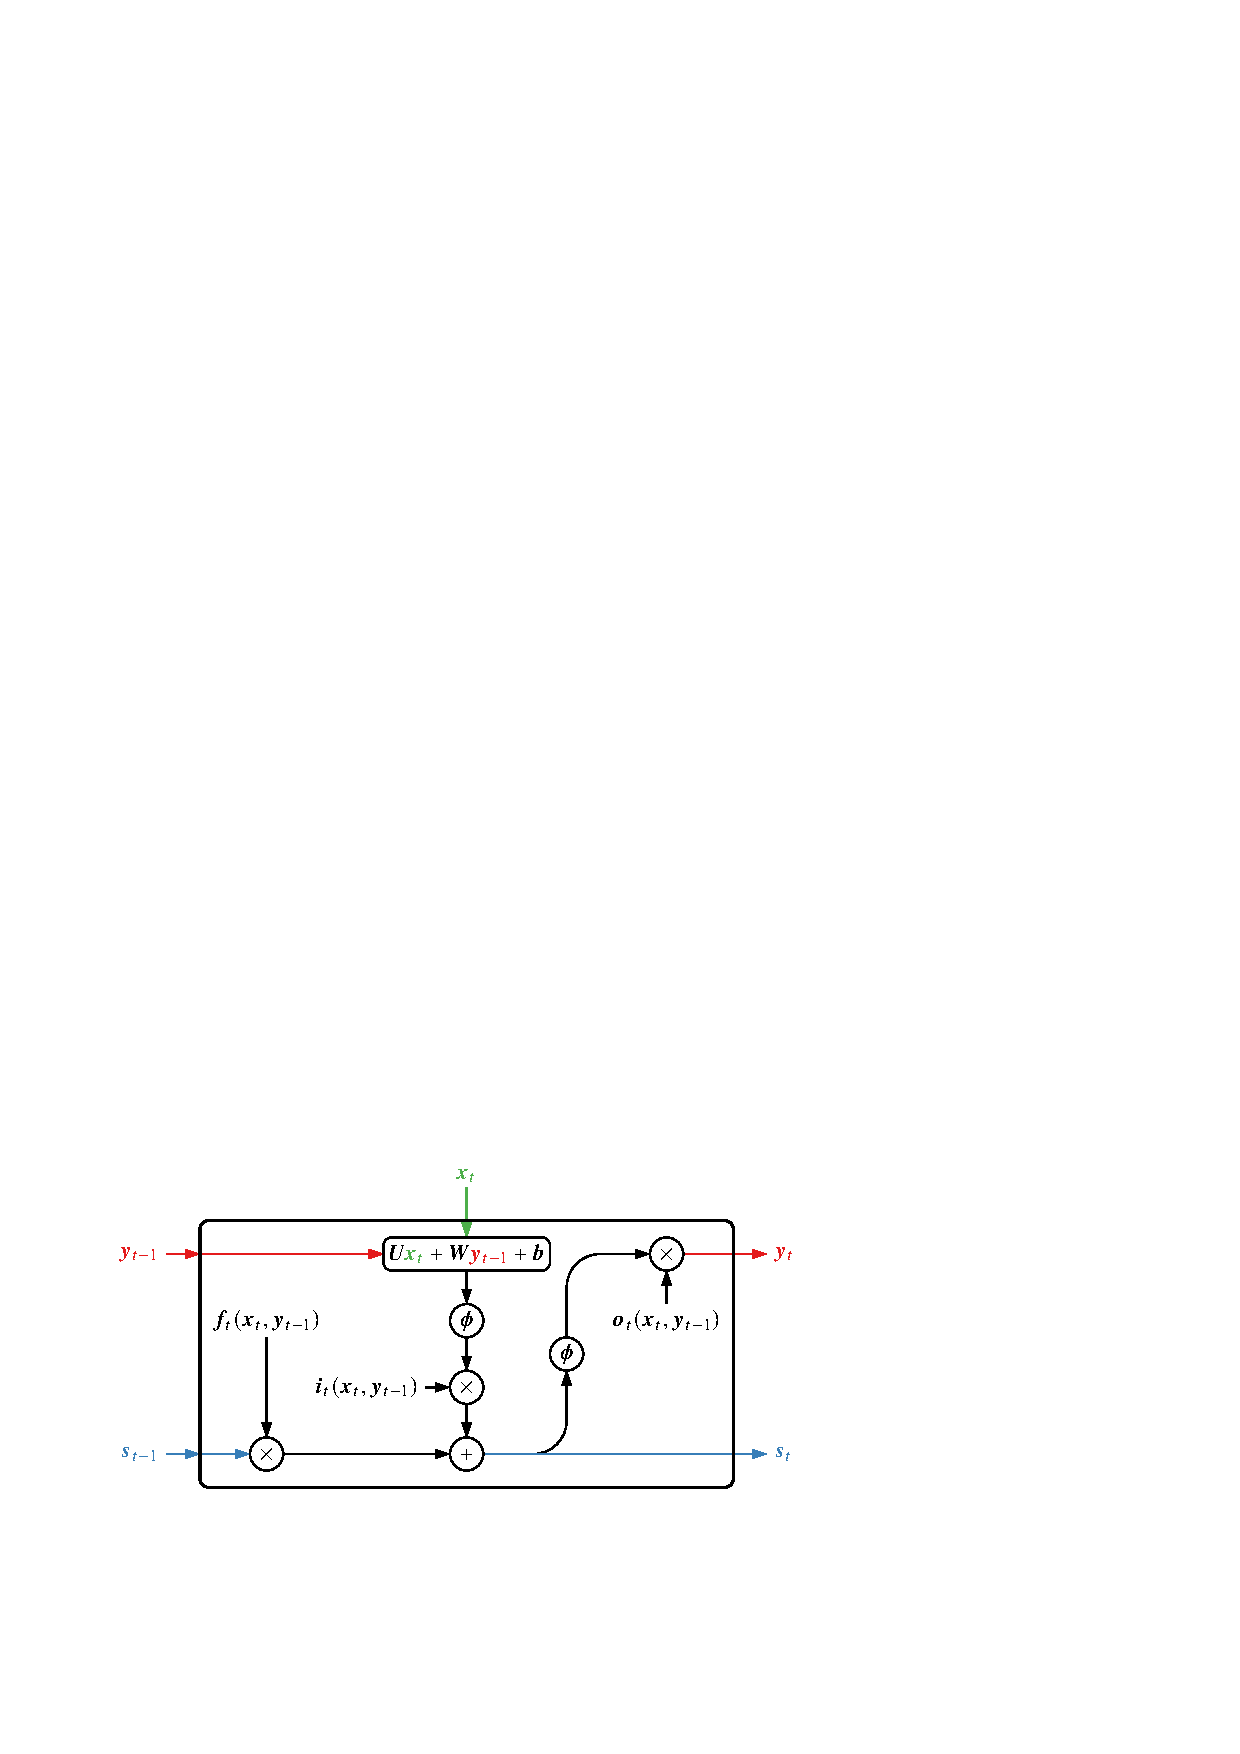
\includegraphics[scale=1.0]{ml/lstm}

  \caption{Computational graph of a single LSTM cell for time step
    $t$. Operations in circles represent element-wise multiplication
    ($\times$), element-wise addition ($+$), and element-wise application of the
    $\tanh$ activation function ($\myvec{\phi}$).
  }
  \label{fig:lstm}
\end{figure}










Maybe say that the RNN as described here is directional. (There are
bi-directional RNNs which are not used here.)





There are other methods such as \emph{gated recurrent
  units}~\cite{cho2014properties} and also approaches using entirely different
architectures such as \emph{transformers}~\cite{vaswani2017attention}.


dynamic internal state that evolves through time.


- Processing sequence: weights have to be shared.
- Context: need some dynamic internal state that propagates through time

Problems with RNN
- The problem of learning long-term dependencies in recurrent networks

Long short-term memory (LSTM)~\cite{lstm}

\textsc{Keras}~\cite{keras}

%% Goodfellow-et-al-2016,}



three gates: the forget gate, the input gate, and the output gate.


\footnote{The introduction of gates is a solution to what is referred to as the
  \emph{vanishing} or \emph{exploding gradient
    problem}~\cite{hochreiter1991untersuchungen}, which prevents efficient
  training of simpler RNN architectures using gradient-based optimisation
  methods due to exponentially decaying/growing gradients with respect to $t$.}




The activations of the gates control the flow of information










% A input sequence~$(\myvec{x}_{t})_{t = 1}^{N}$ can be processed by connecting
    % repeating the computation depicted in the figure once for
    % connecting $N$ of the depicted cell as depicted horizontally
    % horizontally connecting $N$.




RNN operates on sequences of vectors. The length of the sequence is
variable. Each element of the sequence is typically referred to as a \emph{time
  step}.

Can be unfolded into a feedforward neural network. Main point: The unfolded
layers share their parameters (otherwise the sequences would have to have fixed
length).


Gated RNNs solve the vanishing or exploding gradient problems that plague naive
RNN implementations. Gradients exponentially decay or grow with every time step.


%%% Local Variables:
%%% mode: latex
%%% TeX-master: "../../phd_thesis"
%%% End:


% ==============================================================================
\chapter{Tau Identification with Neural Networks}%
\label{sec:tauid}
% ==============================================================================
This chapter describes a novel algorithm used at the ATLAS experiment to
identify the visible decay products of hadronic \taulepton decays. The algorithm
is applied to \tauhadvis candidates passing \tauhadvis reconstruction and aims
to differentiate between candidates originating from \tauhad (\truetauhadvis)
and those originating from non-\tauhad sources (\faketauhadvis). This step is
necessary since \tauhadvis reconstruction is not optimised to reject
\faketauhadvis but rather to correctly reconstruct \truetauhadvis and maintain
high \tauhadvis reconstruction efficiencies.
% More generally, the process of distinguishing between true- and \faketauhadvis
% is called \tauid.

The dominant source of \faketauhadvis at the ATLAS experiment are quark- or
gluon-initiated jets due to their similarity to the hadronic and jet-like
signature of \tauhadvis. Electrons can be another, less abundant source of
\faketauhadvis that have to be distinguished from \truetauhadvis using a
dedicated algorithm (\emph{electron veto}). This chapter is concerned with the
former source of \faketauhadvis and, in particular, with classifying the source
of \tauhadvis candidates as either originating from \tauhad or from quark- or
gluon-initiated jets. This process is referred to as \tauid hereafter.
% More motivation? Say something about reducing mis-identification
% rates to reduce backgrounds?

A number of features can be exploited to differentiate between
\tauhadvis candidates originating from \tauhad and quark- or
gluon-initiated jets:
\begin{description}

\item[\taulepton mass] The \taulepton has a mass of
  \SI{1.777}{\GeV}~\cite{pdg2020} and is therefore sufficiently massive to decay
  hadronically while still having a small mass compared to the energy scales
  typically studied at the ATLAS experiment.

  The \taulepton mass can be used as a feature directly by considering the
  invariant mass of the visible daughter particles of hadronic \taulepton
  decays. Ignoring reconstruction effects, this invariant mass is bounded by the
  mass of the \taulepton. This is not the case for \tauhadvis candidates
  originating from quark- or gluon-initiated jets, which do not have a strict
  upper bound.

  The features described hereafter are consequences of, or closely
  related to the mass of the \taulepton.

\item[Particle multiplicity] Hadronic decays of \tauleptons produce
  few (visible) daughter particles. Most decays produce one or three
  charged hadrons (most frequently $\pi^{\pm}$) and zero to two
  neutral pions.
  % Ellis, Stirling, Webber: 6.4 Quark and gluon jet differences
  In contrast, the average multiplicity of charged and neutral particles in jets
  originating from the fragmentation of partons produced in hard scattering
  interactions is large and increases with the momentum of the
  jet~\cite{Ellis:1996mzs,STDM-2015-12}. Therefore, particle multiplicity
  requirements are effective at rejecting \tauhadvis candidates originating from
  quark- or gluon-initiated jets.\footnote{Gluon-initiated jets have, on
    average, a larger particle multiplicity and a broader angular distribution
    of particles compared to quark-initiated jets due to the larger effective
    colour charge of gluons~\cite{Ellis:1996mzs}. Consequently, quark-initiated
    jets are more likely to be reconstructed and misidentified as \tauhadvis
    candidates.}

\item[Collimated daughter particles] The \tauhadvis candidates typically
  considered by analyses at the ATLAS experiment have transverse momenta
  exceeding \SI{20}{\GeV}. At these momentum scales the decay products of
  \tauleptons are collimated due to the Lorentz boost of the \taulepton. This
  leads to the characteristic detector signature of a narrow jet with few
  visible particles. Requirements on the isolation\footnote{Isolation of a
    reconstructed object refers to a lack of activity in the vicinity of the
    object. The activity is often quantified using reconstructed
    charged-particle tracks or topo-clusters in a cone or annulus surrounding
    the object.} of \tauhadvis candidates allow to reject candidates originating
  from quark- or gluon-initiated jets, which have a wider angular distribution
  of hadrons.

  % Mean flight path of a p = 20 GeV tau is
  % L = beta * gamma * c * tau = p/m0 * 87mu ~ 1mm
\item[\taulepton lifetime] The \taulepton has a proper lifetime of
  \SI{2.9e-13}{\second} ($c \tau = \SI{87}{\micro\metre}$)~\cite{pdg2020} and
  thus typically travels for a few millimetres inside the beampipe before
  decaying. The distance traversed by the \taulepton before its decay results in
  a decay vertex that is displaced from the PV. For \taulepton decay modes with
  three charged hadrons, this secondary vertex can be reconstructed and its
  displacement from the PV determined. For decay modes with only one charged
  hadron, the secondary vertex cannot be reconstructed directly. However, the
  longitudinal and transverse impact parameters of the reconstructed
  charged-hadron track can be used to gauge the incompatibility of the track
  with the PV, thus being sensitive to displaced decays of \tauleptons.

  Features sensitive to the \taulepton lifetime can be used to distinguish
  \tauhad from light-quark- or gluon-initiated jets in which hadrons are
  produced promptly at the PV. An exception are jets originating from $b$- and
  $c$-quarks. These also contain displaced decays of $b$- or $c$-flavoured
  hadrons. However, the other features remain effective in discerning \tauhad
  from $b$- and $c$-jets.

\end{description}
Prior to the introduction of the method described in this chapter, the
ATLAS collaboration used BDTs as binary classifiers using high-level
discriminating variables, i.e.\ variables purposefully constructed for
the classification task, as inputs.

A method of performing \tauid using neural networks that combines the
information of high-level discriminating variables with information from
reconstructed charged-particle tracks and topo-clusters in the calorimeters is
presented. Tracks and topo-clusters in the vicinity of \tauhadvis candidates and
their associated features are included as inputs to neural networks. Since the
number of tracks and topo-clusters associated to \tauhadvis candidates varies,
an RNN architecture is used that allows to operate on sequences of varying
length. The method is referred to as the RNN \tauid hereafter.

The RNN \tauid algorithm was initially proposed in Ref.~\cite{cdeutsch-master}
motivated by a similar approach developed for track impact parameter based
$b$-tagging~\cite{ATL-PHYS-PUB-2017-003}. The algorithm was implemented in the
reconstruction software of the ATLAS collaboration~\cite{ATL-SOFT-PUB-2021-001}
and some of the results presented in this chapter were published in
Ref.~\cite{ATL-PHYS-PUB-2019-033}.
% The RNN \tauid was adopted by the ATLAS collaboration as the recommended
% \tauid algorithm for analyses using the \SI{139}{\per\femto\barn}
% \pp~collision dataset recorded with the ATLAS detector during Run~2 of the
% LHC.

This chapter is structured as follows: The simulated events used for the
development and performance evaluation of \tauid are introduced in
\Cref{sec:tauid_mc}. The identification method based on RNN is described in
\Cref{sec:tauid_rnn}. Its performance is estimated based on simulation and
compared to the BDT-based approach in \Cref{sec:tauid_perf}.
\Cref{sec:tauid_conclusion} concludes and gives an outlook on possible future
developments.

%%% Local Variables:
%%% mode: latex
%%% TeX-master: "../../phd_thesis"
%%% End:

\section{Simulated Event Samples}%
\label{sec:tauid_mc}

The tau reconstruction and identification algorithms employed at the ATLAS
experiment for Run~2 of the LHC were developed using simulated events that
provide samples of \tauhadvis candidates. For \tauid, simulated
$\gammastar \to \tautau$ and dijet events are used, yielding samples of true-
and \faketauhadvis, respectively.

% y->tautau:
% https://gitlab.cern.ch/atlas-physics/pmg/infrastructure/mc15joboptions/-/blob/master/share/DSID425xxx/MC15.425200.Pythia8EvtGen_A14NNPDF23LO_Gammatautau_MassWeight.py
An artificial $\gammastar \to \tautau$ event sample was generated
using \PYTHIA[8.212]~\cite{Sjostrand:2014zea} for the matrix element
calculation at leading order (LO), parton showering, hadronisation,
and \taulepton decays. The contribution of the $Z$ boson propagator to
the hard scattering process was removed to provide an unpolarised
sample of \tauleptons. In addition, the cross section of the process
was modified at generator-level to enhance the number of events with
high invariant $\tautau$ masses to increase the number of \tauhadvis
candidates with large transverse momenta. Both \tauleptons
are enforced to decay hadronically to minimise statistical
uncertainties from the size of the \truetauhadvis sample.

% Di-jet samples: JZ1W up to JZ6W
% https://gitlab.cern.ch/atlas-physics/pmg/infrastructure/mc15joboptions/-/blob/master/share/DSID361xxx/MC15.361021.Pythia8EvtGen_A14NNPDF23LO_jetjet_JZ1W.py
Dijet events are generated using \PYTHIA[8.186]~\cite{Sjostrand:2014zea} for the
matrix element calculation at LO, parton showering, and hadronisation. The
generation is performed in slices of \pT of the leading jet (anti-\kt with
$R = 0.6$) constructed from generator-level particles. Slices with large jet
transverse momenta are oversampled to increase the number of events with jets
(\faketauhadvis) of large transverse momentum.

The $\gammastar \to \tautau$ and dijet samples use the A14 set of tuned
parameters for \PYTHIA[8]~\cite{ATL-PHYS-PUB-2014-021} and the
\NNPDF[2.3lo]~\cite{Ball:2012cx} set of parton distribution functions (PDFs).
Decays of hadrons containing $b$- or $c$-quarks are simulated using
\EVTGEN[v1.2.0]~\cite{Lange:2001uf}. The contamination of the hard scattering
interaction with soft, inelastic proton--proton collision events is accounted
for by overlaying the event with additional minimum-bias events. The response of
the ATLAS detector is simulated for all generated
events~\cite{SOFT-2010-01}. Subsequently, events are reconstructed from the
simulated detector response using the \textsc{Athena} software
suite~\cite{ATL-SOFT-PUB-2021-001}.


\subsection{\tauhadvis Candidate Selection}
\label{sec:tauid_candidate_selection}

The simulated events are used to construct samples of \tauhadvis candidates for
the development and performance evaluation of \tauid algorithms. Only candidates
passing the \tauhadvis reconstruction are considered and the following
selections are applied in addition:
\begin{itemize}

\item The number of \emph{core} tracks (\Ntracks) of the \tauhadvis candidate is
  either one or three. These are referred to as 1- or 3-prong \tauhadvis
  candidates, respectively.

\item The (visible) transverse momentum of the candidate needs to
  fulfil $\pT > \SI{20}{\GeV}$.

\item The \tauhadvis candidate needs to be within $|\eta| < 2.5$ but
  outside the transition region between barrel and end-cap
  electromagnetic calorimeters given by $1.37 < |\eta| < 1.52$.

\end{itemize}
In addition, reconstructed \tauhadvis candidates from
$\gammastar \to \tautau$ events are required to be geometrically
matched to a \tauhad at generator-level ($\Delta R < 0.2$).
% And the reco cuts are required to be fulfilled at truth-level.
All efficiencies and rejection factors given in the remainder of this
chapter do not include the effects of \tauhadvis reconstruction or the
selections outlined above.

The $\gammastar \to \tautau$ and dijet events provide samples of
true- and \faketauhadvis with a size of 20 million and 46 million
candidates, respectively. The distributions of \tauhadvis candidate
\pT is shown for both samples and separately for 1- and 3-prong
candidates in~\Cref{fig:tauid_candidate_pt}. The difference in \pT
spectra between 1- and 3-prong \truetauhadvis in
\Cref{fig:tauid_candidate_pt_gammastar} results from a reduction in
track association efficiency for 3-prong \tauhadvis candidates with
increasing candidate \pT due to the decrease in angular separation of
charged hadrons from the \taulepton decay. In contrast, the \pT
spectrum of \tauhadvis candidates from dijet events, depicted in
\Cref{fig:tauid_candidate_pt_dijet}, shows a heavier tail towards
large \pT for 3-prong candidates due to the increase of the hadron
multiplicity in jets with jet \pT. For the development and performance
evaluation of \tauid algorithms, the sample of \faketauhadvis
candidates is re-weighted, separately for 1- and 3-prong candidates,
to match the \pT spectrum of \truetauhadvis from
$\gammastar \to \tautau$.

\begin{figure}[htbp]
  \begin{subfigure}{0.498\textwidth}
    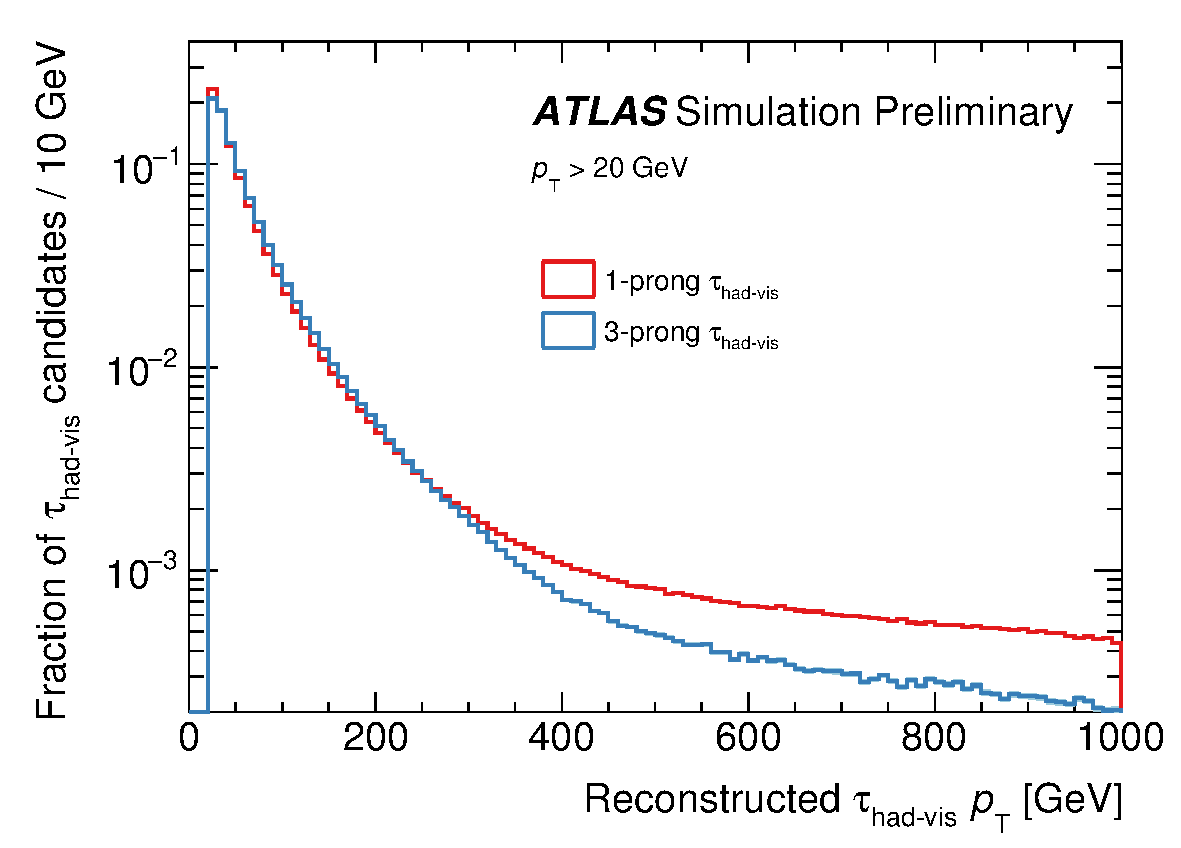
\includegraphics[width=\textwidth]{tauid/pubnote/taupt_gammastar}
    \subcaption{True-\tauhadvis from $\gammastar \to \tautau$ events}%
    \label{fig:tauid_candidate_pt_gammastar}
  \end{subfigure}\hfill%
  \begin{subfigure}{0.498\textwidth}
    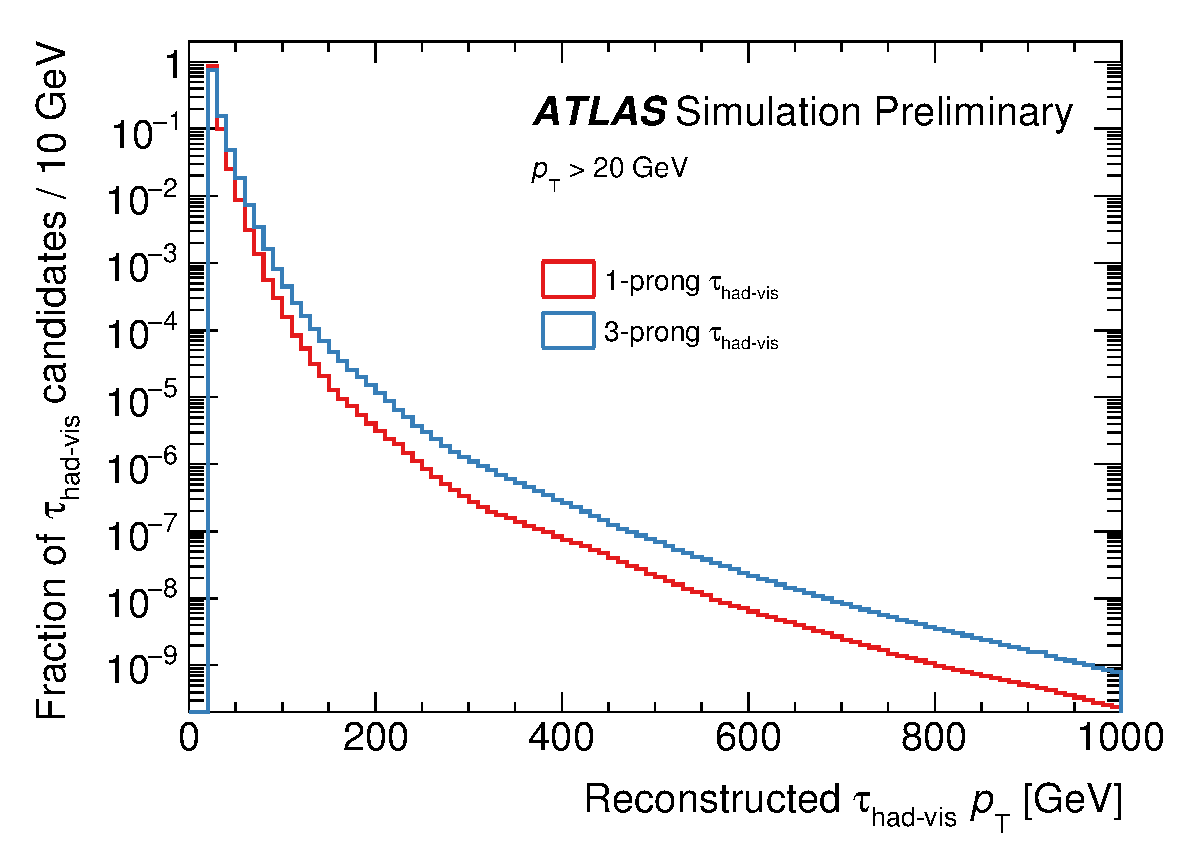
\includegraphics[width=\textwidth]{tauid/pubnote/taupt_dijet}
    \subcaption{Fake-\tauhadvis from dijet events}%
    \label{fig:tauid_candidate_pt_dijet}
  \end{subfigure}

  \caption[Transverse momentum distribution of \tauhadvis candidates in
  $\gammastar \to \tautau$ and dijet events.]{Transverse momentum distributions
    of 1- and 3-prong \tauhadvis candidates in $\gammastar \to \tautau$ (a) and
    dijet events (b). Statistical uncertainties are shown as coloured bands
    surrounding the central value. The figures are taken from
    Ref.~\cite{ATL-PHYS-PUB-2019-033}.}%
  \label{fig:tauid_candidate_pt}
\end{figure}


%%% Local Variables:
%%% mode: latex
%%% TeX-master: "../../phd_thesis"
%%% End:

\section{Tau Identification with Recurrent Neural Networks}%
\label{sec:tauid_rnn}

The RNN \tauid exploits the discrimination power of both high- and low-level
inputs to distinguish \tauhad from quark- or gluon-initiated jets. This approach
aims to avoid a possible loss of information relevant to \tauid when manually
constructing high-level variables from low-level inputs. Specifically,
charged-particle tracks and topo-clusters in the calorimeters, hereafter
abbreviated as tracks and clusters, are included as low-level inputs to the
algorithm. Their inclusion targets the differences in charged- and
neutral-hadron multiplicities and track- and calorimeter-based isolation between
true and \faketauhadvis. Tau identification is performed separately for 1- and
3-prong \tauhadvis candidates due to their distinct signatures.


\subsection{Input Variables}

The input variables included in the RNN \tauid algorithm are summarised
in~\Cref{tab:tauid_input_variables}. Three categories of inputs are considered:
high-level, track, and cluster inputs. High-level inputs are observables
directly associated to \tauhadvis candidates. Track and cluster inputs refer to
observables of tracks and clusters that are associated to a \tauhadvis
candidate. In the following, a description of the input variable selection and
track/cluster association is given.

\begin{table}[htbp]
  \centering

  \caption[Input variables used for the RNN \tauid.]{Summary of input variables
    used for the RNN \tauid. The local hadronic calibration~\cite{PERF-2014-07}
    is used to calibrate jets, clusters, and \tauhadvis candidates unless
    otherwise noted. Definitions of geometrical topo-cluster moments measuring
    the location and shape of clusters ($\lambda$, $\langle \lambda^2 \rangle$,
    $\langle r^2 \rangle$) are given in Ref.~\cite{PERF-2014-07}. Variables
    using cell-level calorimeter information only consider cells that are part
    of topo-clusters for noise suppression. $\dagger$:~Energy depositions in the
    pre-sampler and first two layers of the electromagnetic calorimeters that
    are part of topo-clusters are abbreviated as ``EM clusters''. The table is
    adapted from Ref.~\cite{ATL-PHYS-PUB-2019-033}.}%
  \label{tab:tauid_input_variables}

  \resizebox{0.99\textwidth}{!}{
    \renewcommand{\arraystretch}{1.3}

\begin{tabular}{clp{13.5cm}}
  \toprule
  & Variable & Description \\
  \midrule
  \parbox[t]{2mm}{\multirow{11}{*}{\rotatebox[origin=c]{90}{High-level inputs\hspace*{65pt}}}}
  & $p_\text{T}$
  & Calorimeter-based estimate of \tauhadvis candidate \pT. \\

  & $f_\text{cent}$
  & Ratio of \ET deposited in calorimeter cells (at EM scale) in cones of $\Delta R < 0.1$ and $\Delta R < 0.2$ about the \tauhadvis axis. \\

  & $f_\text{leadtrack}^{-1}$
  & Ratio of \ET deposited in calorimeter cells (at EM scale) in a cone of $\Delta R < 0.2$ about the \tauhadvis axis and the \pT of the \pT-leading \emph{core} track. \\

  & $\Delta R_\text{max}$
  & Maximum $\Delta R$ between \emph{core} tracks and the \tauhadvis axis. \\

  & $|S_\text{leadtrack}|$
  & Transverse impact parameter significance of the \pT-leading track. Only considered for 1-prong \tauhadvis candidates.\\

  & $S_\text{T}^\text{flight}$
  & Transverse flight path significance. Only considered for 3-prong \tauhadvis candidates. \\

  & $f_\text{iso}^\text{track}$
  & Ratio of the scalar sum of \pT of \emph{isolation} tracks and the scalar sum of \pT of \emph{core} and \emph{isolation} tracks. \\

  & $f_\text{track}^\text{EM}$
  & Ratio of the energy in EM clusters$^\dagger$ and the scalar sum of momenta of \emph{core} tracks. \\

  & $p_\text{T}^\text{EM+track}/\pT$
  & \pT of the \tauhadvis estimated from the momenta of \emph{core} tracks and the two most energetic EM clusters$^\dagger$ divided by the \pT of the calorimetric measurement. \\

  & $m^\text{EM+track}$
  & Invariant mass of the system of \emph{core} tracks and the two most energetic EM clusters$^\dagger$. \\

  & $m^\text{track}$
  & Invariant mass of the system of \emph{core} tracks. Only considered for 3-prong \tauhadvis candidates. \\
  \midrule
  \parbox[t]{2mm}{\multirow{9}{*}{\rotatebox[origin=c]{90}{Track inputs\hspace*{10pt}}}}
  & $p_\text{T}^\text{jet seed}$
  & \pT of the jet seeding the \tauhadvis candidate. \\

  & $p_\text{T}^\text{track}$
  & \pT of the track. \\

  & $\Delta\eta^\text{track}$
  & Difference in $\eta$ between track and \tauhadvis axis. \\

  & $\Delta\phi^\text{track}$
  & Angle between track and \tauhadvis axis in the transverse plane. \\

  & $|d_0^\text{track}|$
  & Absolute value of the transverse track impact parameter. \\

  & $|z_0^\text{track} \sin\theta|$
  & Absolute value of the product of longitudinal track impact parameter and the sine of the polar angle of the track. \\

  & $N_\text{IBL hits}$
  & Number of hits on the track in the IBL. \\

  & $N_\text{Pixel hits}$
  & Number of hits on the track in pixel detector layers. \\

  & $N_\text{SCT hits}$
  & Number of hits on the track in SCT layers. \\

  \midrule
  \parbox[t]{2mm}{\multirow{7}{*}{\rotatebox[origin=c]{90}{Cluster inputs}}}
  & $p_\text{T}^\text{jet seed}$
  & \pT of the jet seeding the \tauhadvis candidate. \\

  & $E_\text{T}^\text{cluster}$
  & \ET of the cluster. \\

  & $\Delta\eta^\text{cluster}$
  & Difference in $\eta$ between cluster and \tauhadvis axis. \\

  & $\Delta\phi^\text{cluster}$
  & Angle between cluster and \tauhadvis axis in the transverse plane. \\

  & $\lambda_\mathrm{cluster}$
  & Longitudinal distance of the cluster barycentre from the calorimeter front face. \\

  & $\langle \lambda^2\rangle_{\text{cluster}}$
  & Second longitudinal cluster moment. \\

  & $\langle r^2\rangle_{\text{cluster}}$
  & Second radial cluster moment. \\
  \bottomrule
\end{tabular}

%%% Local Variables:
%%% mode: latex
%%% TeX-master: "../phd_thesis"
%%% End:

  }
\end{table}

\subsubsection{High-Level Input Variables}

The selection of high-level input variables is based on the variables used in
the BDT-based \tauid algorithm developed by the ATLAS
collaboration~\cite{ATL-PHYS-PUB-2015-045}, which was updated in
Ref.~\cite{cdeutsch-master} for the new \tauhadvis reconstruction techniques
deployed during Run~2 of the LHC. The BDT \tauid uses only the high-level
variables summarised in~\Cref{tab:tauid_input_variables} as inputs and serves as
a baseline for comparison with the RNN-based algorithm.

Variables sensitive to the lifetime and mass of the \taulepton
($|S_{\text{T}}^{\text{flight}}|$, $|S_{\text{leadtrack}}|$,
$m^{\text{track}}$), the isolation of \tauhadvis in the tracking
system ($f_{\text{iso}}^{\text{track}}$) and the calorimeters
($f_{\text{cent}}$), and combinations of track- and calorimeter-based
isolation ($f_{\text{track}}^{\text{EM}}$,
$p_{\text{T}}^{\text{EM+track}} / \pT$) are among the most important
high-level variables included in the \tauid algorithms. Three
exemplary distributions are shown in~\Cref{fig:tauid_high_level_vars}.


\begin{figure}[htbp]
  \centering

  \begin{subfigure}{0.33\textwidth}
    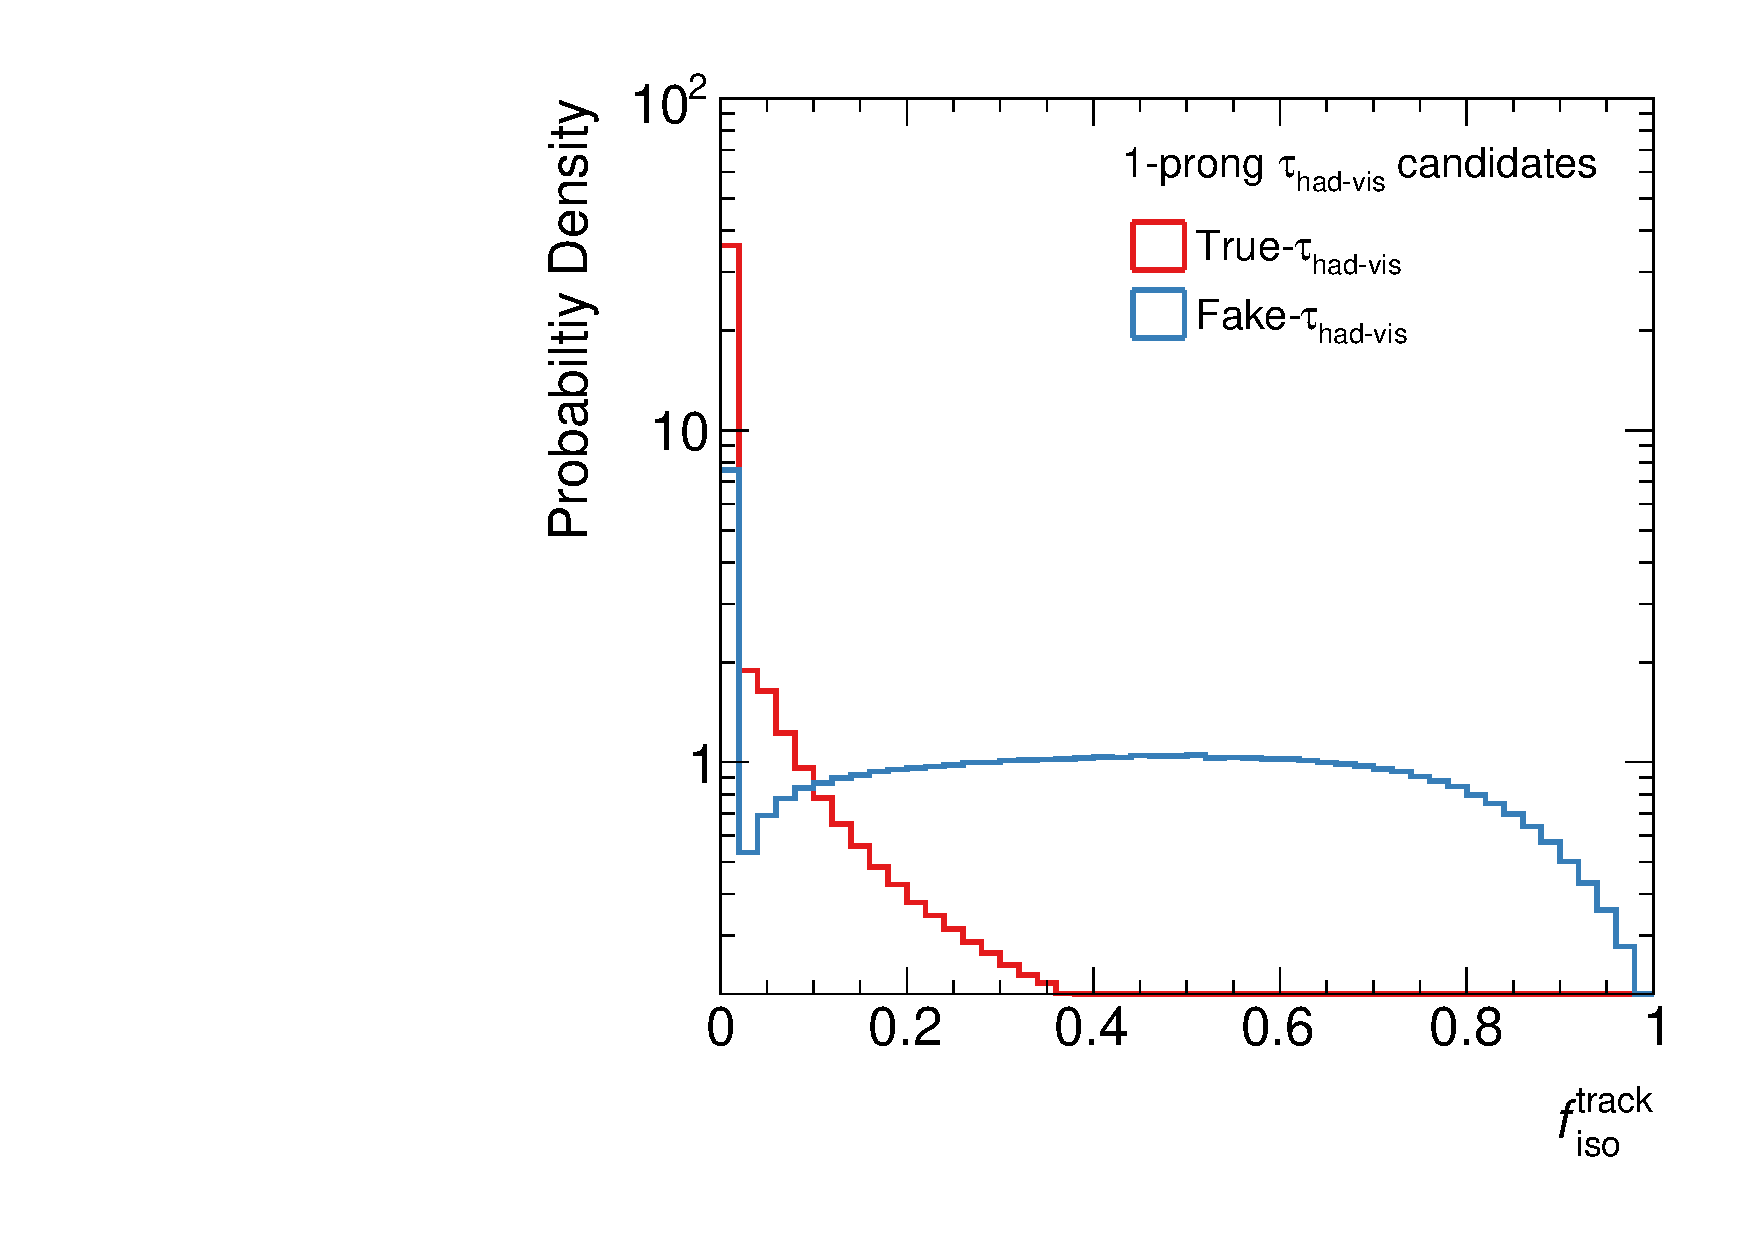
\includegraphics[width=\textwidth]{tauid/invars/invars_sumpttrkfrac_1P}
    \subcaption{}
  \end{subfigure}\hfill%
  \begin{subfigure}{0.33\textwidth}
    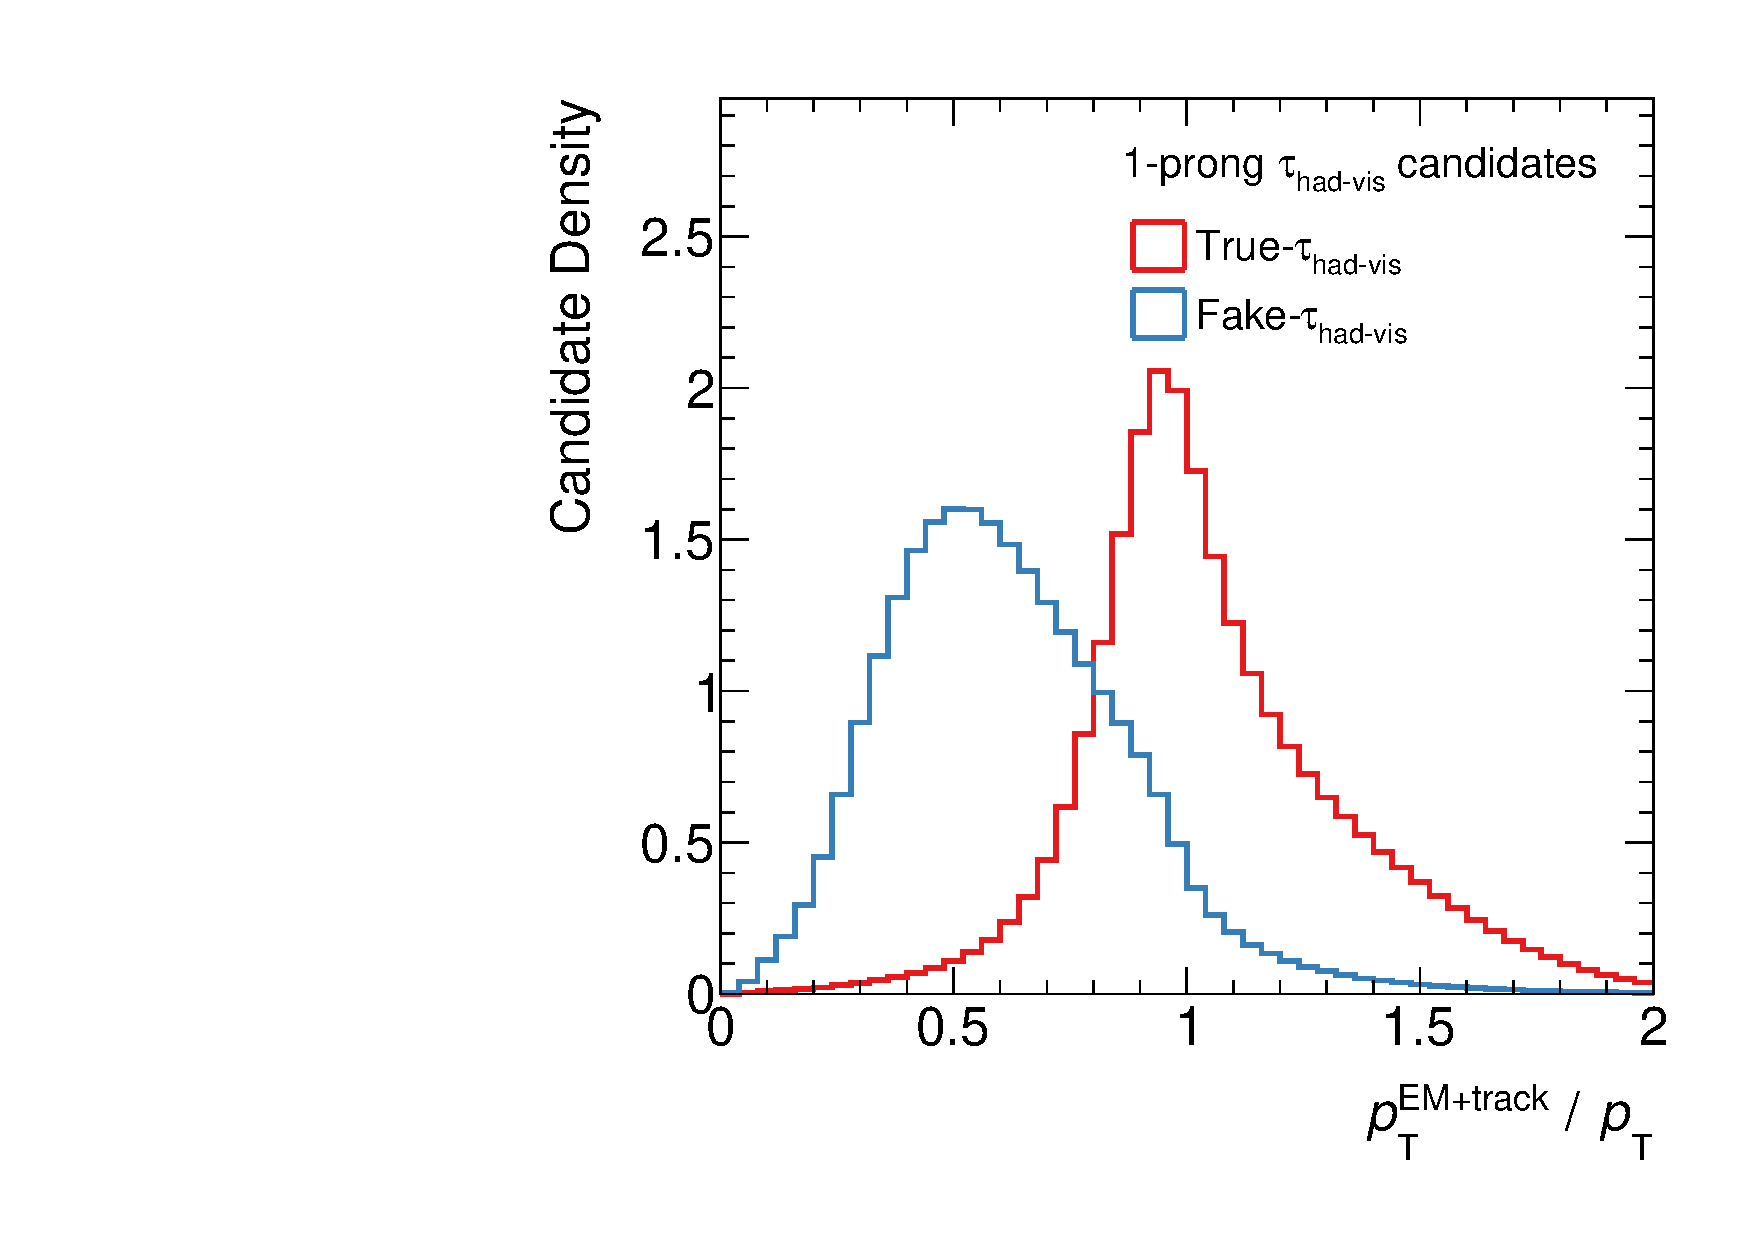
\includegraphics[width=\textwidth]{tauid/invars/invars_ptratioeflowapprox_1P}
    \subcaption{}
  \end{subfigure}\hfill%
  \begin{subfigure}{0.33\textwidth}
    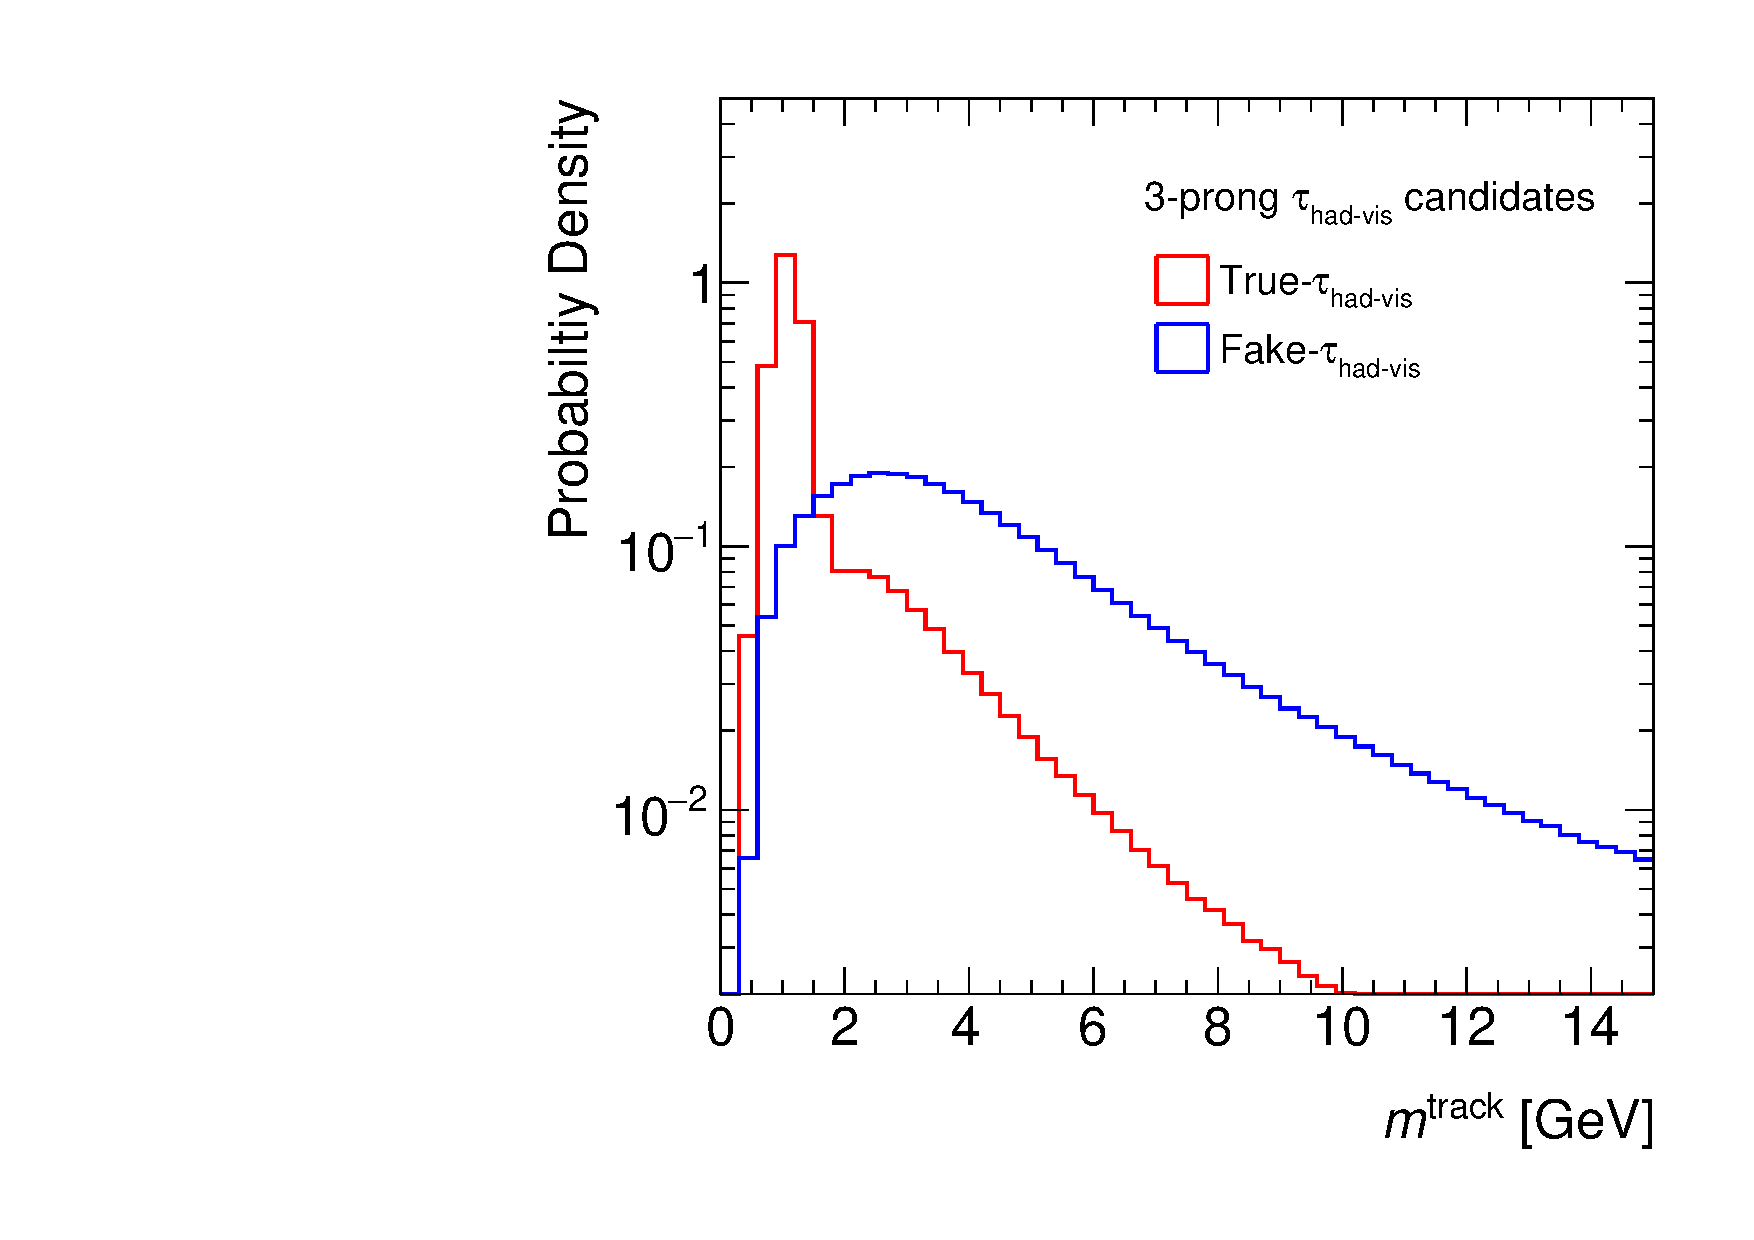
\includegraphics[width=\textwidth]{tauid/invars/invars_masstrksys_3P}
    \subcaption{}
  \end{subfigure}

  \caption[Distributions of exemplary high-level input variables used for
  \tauid.]{Distributions of exemplary high-level input variables used for
    \tauid. (a):~The ratio of the scalar sum of \pT of tracks classified as
    \emph{isolation} with respect to tracks classified as \emph{core} or
    \emph{isolation}. (b):~The ratio of \tauhadvis candidate \pT estimated using
    a simplified particle flow approach and the purely calorimeter-based
    measurement (cf.~\Cref{tab:tauid_input_variables}). (c):~The mass of the
    system of \emph{core} tracks for 3-prong \tauhadvis candidates.}%
  \label{fig:tauid_high_level_vars}
\end{figure}


\subsubsection{Track Input Variables}

Reconstructed tracks with $\pT > \SI{500}{\MeV}$ and within a cone of
$\Delta R < 0.4$ about the \tauhadvis candidate axis are considered as inputs to
the RNN \tauid. No selections are applied on the quality and impact parameters
of reconstructed tracks, thus the inputs include tracks from the \tauleptonC
decay as well as fake tracks and tracks from pile-up. Instead, track quality
criteria ($N_{\text{IBL hits}}$, $N_{\text{Pixel hits}}$, $N_{\text{SCT hits}}$)
and track impact parameters ($|d_0^{\text{track}}|$,
$|z_0^{\text{track}} \sin\theta|$) are included as observables of tracks.

In addition, several other track-level observables, summarised
in~\Cref{tab:tauid_input_variables}, are included. Among the most important
variables are the transverse momenta of reconstructed tracks
($p_{\text{T}}^{\text{track}}$) and their angular separation from the \tauhadvis
candidate axis ($\Delta \eta^{\text{track}}$, $\Delta
\phi^{\text{track}}$). These variables are included to probe the isolation
properties of \tauhadvis candidates. A special case is the
$p_{\text{T}}^{\text{jet seed}}$ variable, the \pT of the jet seeding the
\tauhadvis candidate, which is not a track property but is still included as an
observable for every track. This is done to provide an approximate \pT-scale of
the jet already at the level of individual input tracks. Exemplary distributions
of the transverse momenta of the three \pT-leading tracks normalised to
$p_{\text{T}}^{\text{jet seed}}$ are shown
in~\Cref{fig:tauid_low_level_variables_track} for 1-prong \tauhadvis
candidates.%\todo{Add 2D plots in appendix?}

% \todo[inline]{It would be nice to have 2D plots of leading track \pT vs
% sub-leading track \pT in the appendix. Same for cluster \ET.}

\begin{figure}[htbp]
  \centering

  \begin{subfigure}{0.33\textwidth}
    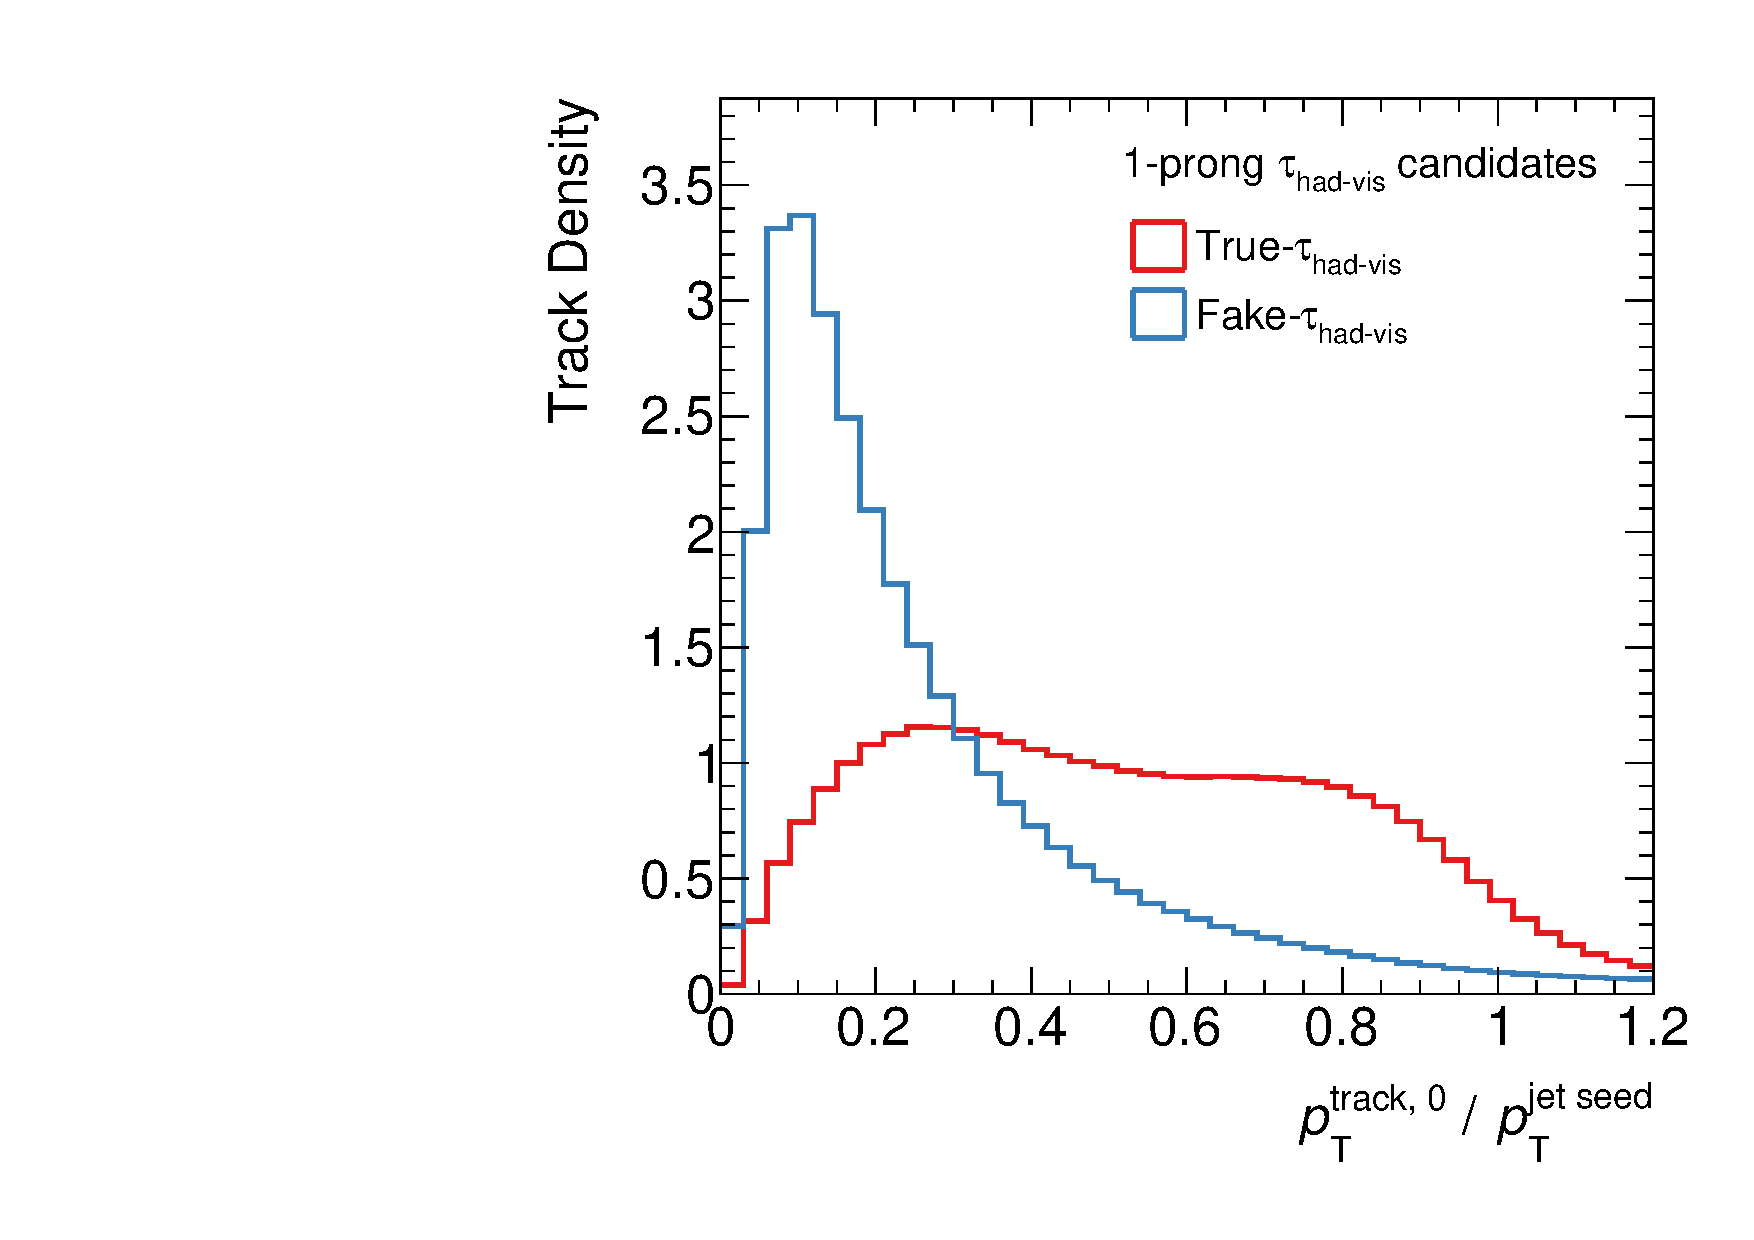
\includegraphics[width=\textwidth]{tauid/invars/invars_trk0relpt_1P}
    \subcaption{}%
    \label{fig:tauid_low_level_variables_track0}
  \end{subfigure}%
  \begin{subfigure}{0.33\textwidth}
    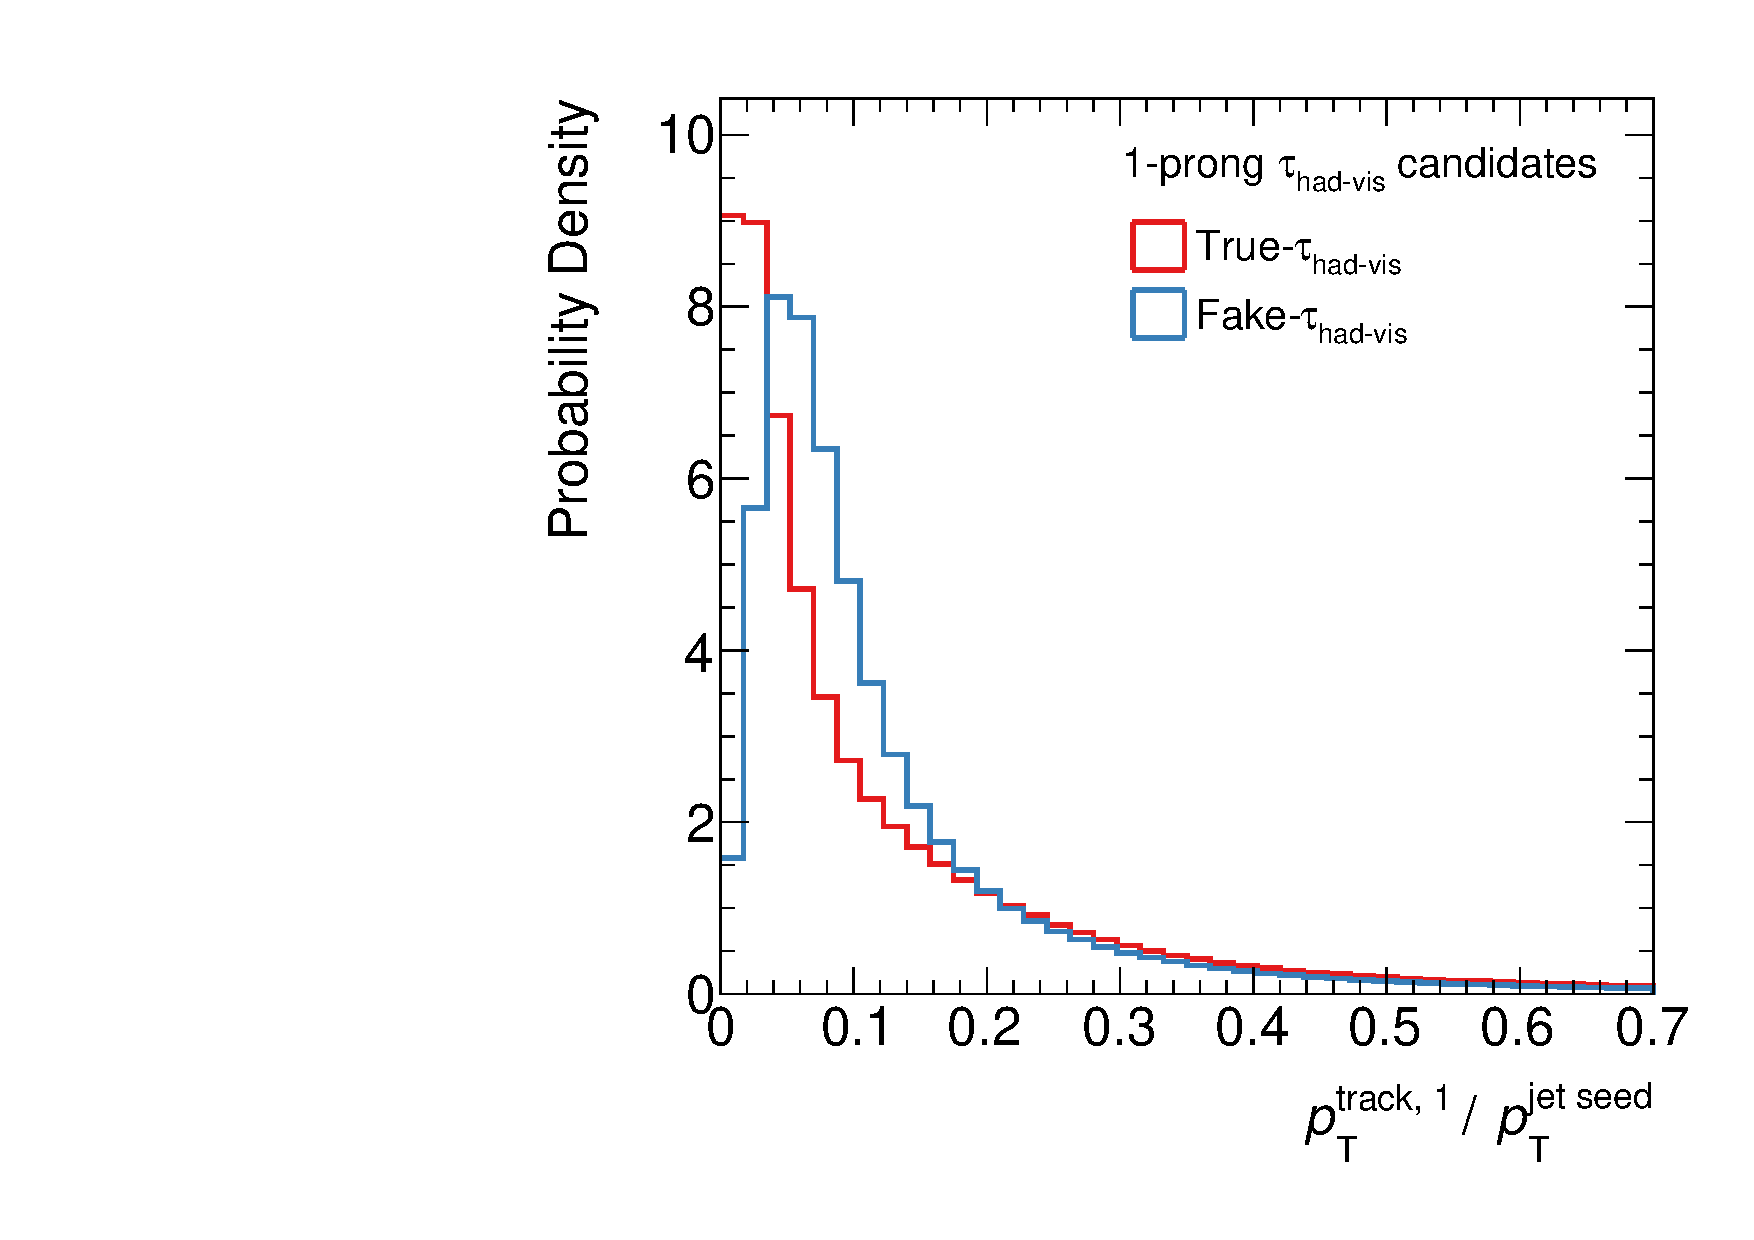
\includegraphics[width=\textwidth]{tauid/invars/invars_trk1relpt_1P}
    \subcaption{}%
    \label{fig:tauid_low_level_variables_track1}
  \end{subfigure}%
  \begin{subfigure}{0.33\textwidth}
    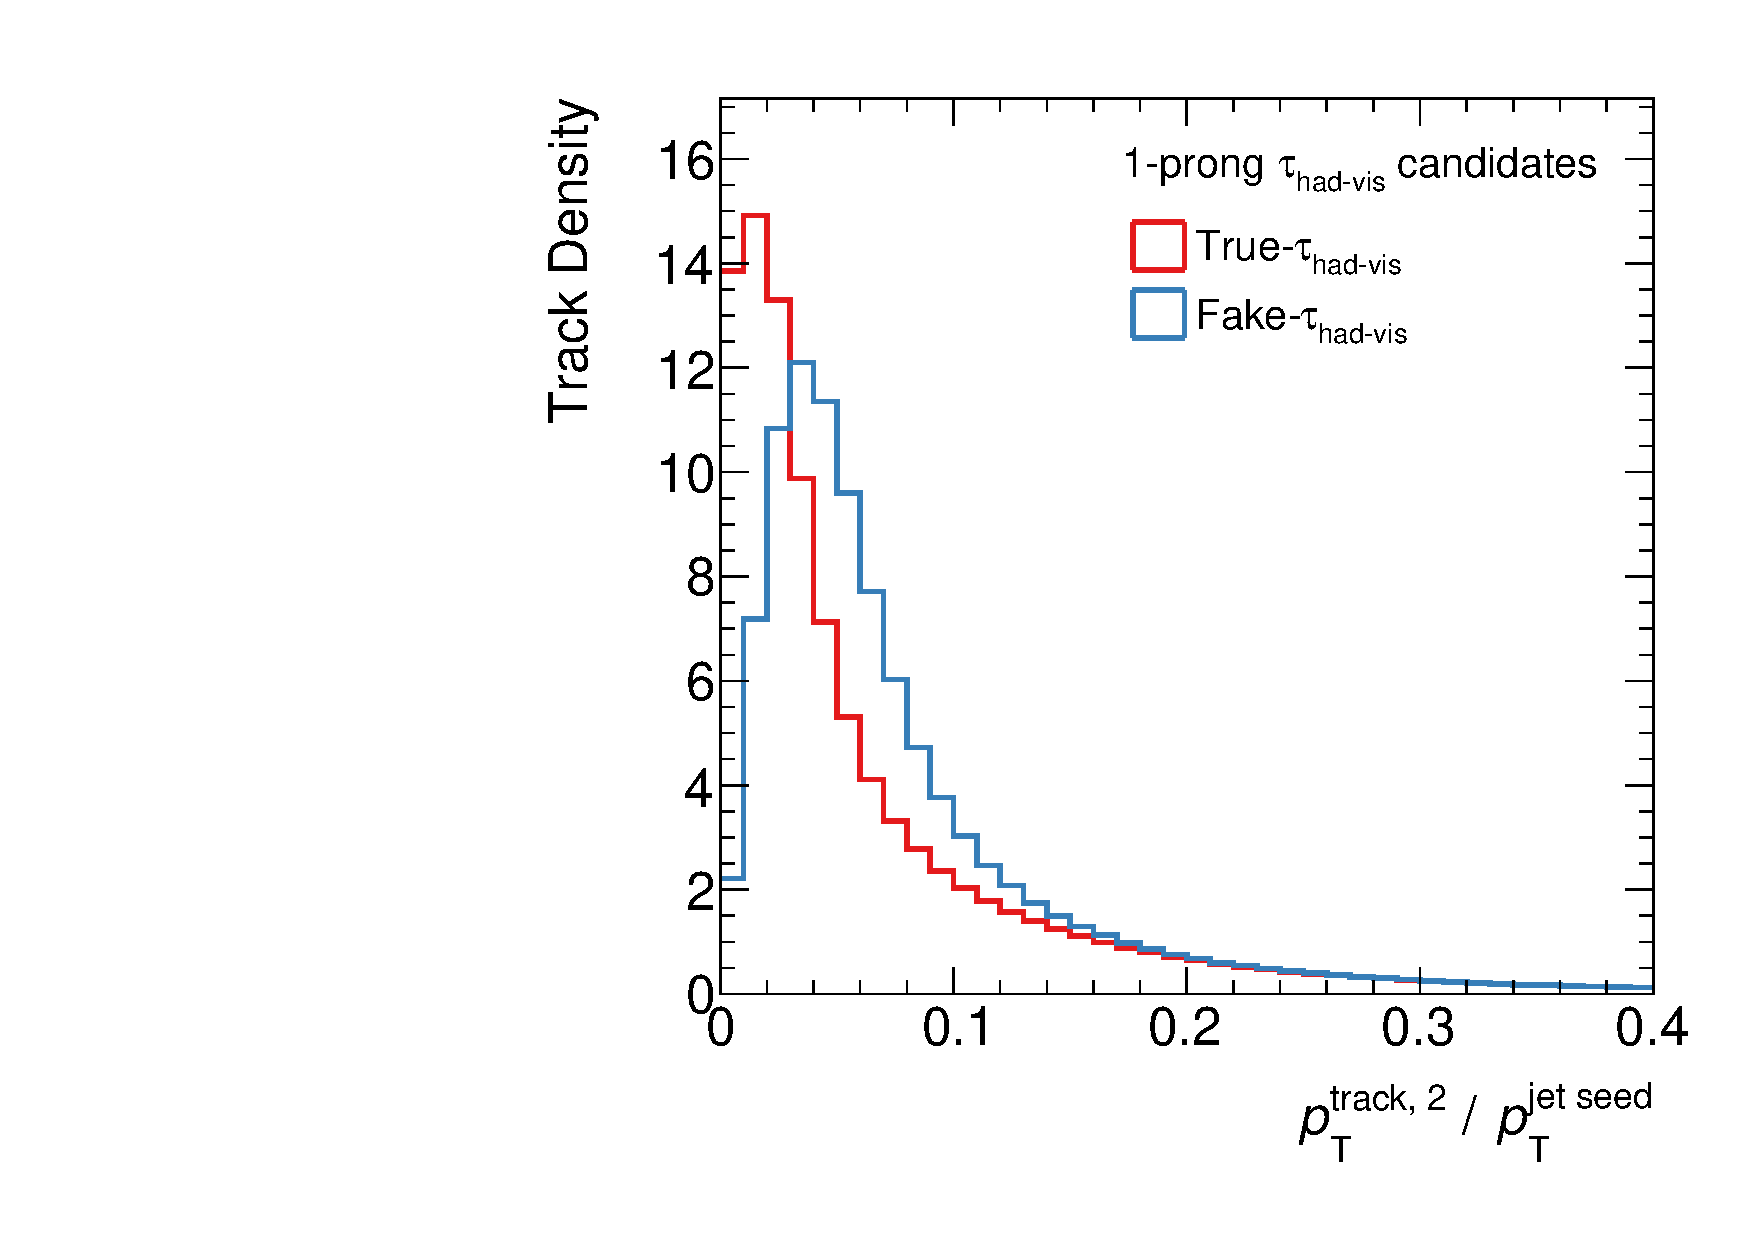
\includegraphics[width=\textwidth]{tauid/invars/invars_trk2relpt_1P}
    \subcaption{}%
    \label{fig:tauid_low_level_variables_track2}
  \end{subfigure}

  \caption[Distributions of the transverse momenta of the three \pT-leading
  tracks associated to 1-prong \tauhadvis candidates.]{Distributions of the
    transverse momenta of the three \pT-leading tracks associated to 1-prong
    \tauhadvis candidates. For illustration purposes, the track \pT are
    normalised to the \pT of the jet seeding the \tauhadvis candidate.}%
  \label{fig:tauid_low_level_variables_track}
\end{figure}

The discrimination power of the RNN \tauid saturates after including the ten
highest-\pT tracks; therefore, the sequence of tracks is truncated at this point
to reduce the computational resources required for training and evaluation of
the networks.


\subsubsection{Cluster Input Variables}

Topo-clusters in the calorimeters are considered as inputs to the RNN \tauid if
they are constituents of the jet seeding the \tauhadvis reconstruction. All
clusters are calibrated using the local hadronic calibration to account for the
non-compensating nature of the calorimeters, energy deposition in calorimeter
cells not part of the cluster, and energy loss in inactive
material~\cite{PERF-2014-07}.

The inclusion of the $E_{\text{T}}^{\text{cluster}}$,
$\Delta \eta^{\text{cluster}}$, $\Delta \phi^{\text{cluster}}$, and
$p_{\text{T}}^{\text{jet seed}}$ observables
(cf.~\Cref{tab:tauid_input_variables}) follow from considerations
similar to those for charged-particle tracks. In addition, information
on the position and shape of showers in the calorimeters is included
in the form of cluster moments~\cite{PERF-2014-07}, targeting the
differences between electromagnetic and hadronic showers. These
cluster moments include the longitudinal location of the cluster
barycentre, $\lambda_{\text{cluster}}$, and the lateral and
longitudinal extension of the cluster,
$\langle r^2 \rangle_{\text{cluster}}$ and
$\langle \lambda^2 \rangle_{\text{cluster}}$, respectively. For
illustration, the \ET of the three \ET-leading clusters is shown
in~\Cref{fig:tauid_low_level_variables_cluster} for 3-prong \tauhadvis
candidates.

\begin{figure}[htbp]
  \centering

  \begin{subfigure}{0.33\textwidth}
    \includegraphics[width=\textwidth]{tauid/invars/invars_cls0relet_3P}
    \subcaption{}%
    \label{fig:tauid_low_level_variables_cluster0}
  \end{subfigure}%
  \begin{subfigure}{0.33\textwidth}
    \includegraphics[width=\textwidth]{tauid/invars/invars_cls1relet_3P}
    \subcaption{}%
    \label{fig:tauid_low_level_variables_cluster1}
  \end{subfigure}%
  \begin{subfigure}{0.33\textwidth}
    \includegraphics[width=\textwidth]{tauid/invars/invars_cls2relet_3P}
    \subcaption{}%
    \label{fig:tauid_low_level_variables_cluster2}
  \end{subfigure}

  \caption[Distributions of the transverse energy of the three \ET-leading
  clusters associated to 3-prong \tauhadvis candidates.]{Distributions of the
    transverse energies of the three \ET-leading clusters associated to 3-prong
    \tauhadvis candidates. For illustration purposes, the cluster \ET are
    normalised to the \pT of the jet seeding the \tauhadvis candidate.}%
  \label{fig:tauid_low_level_variables_cluster}
\end{figure}

The classification performance of the RNN \tauid saturates after the inclusion
of the six highest-\ET clusters, thus the sequence of input clusters is
truncated at this point.


\subsection{Network Architecture}

The network architecture adopted for the RNN \tauid is shown
schematically in~\Cref{fig:tauid_network_architecture}. The network
consists of three branches, each one dedicated to one type of
input. The high-level variables, track inputs, and cluster inputs are
first processed independently in their respective branches. These
branches are then merged and reduced to a single output node that is
used to define the \tauid working points. The network is implemented
using the \textsc{Keras} library~\cite{keras} with the
\textsc{TensorFlow}
backend~\cite{tensorflow2015-whitepaper}.\footnote{\textsc{Keras}
  v2.2.0 and \textsc{TensorFlow} v1.8.0 are used.} Layers use the
default configurations of \textsc{Keras} unless indicated otherwise. A
description of the network architecture is given in the following.

\begin{figure}[htbp]
  \centering

  \vspace*{0.2em}

  \includegraphics[width=0.98\textwidth]{tauid/pubnote/rnn_network_architecture}

  \vspace*{0.2em}

  \caption[Network architecture used for the RNN \tauid algorithm.]{Network
    architecture used for the RNN \tauid algorithm. Individual layers of the
    network are depicted as rectangles. The figure is adapted from
    Ref.~\cite{ATL-PHYS-PUB-2019-033}.}%
  \label{fig:tauid_network_architecture}
\end{figure}

The branch of the network operating on high-level input variables
consists of three fully-connected (\emph{dense}) layers with 128, 128,
and 16 units each. The \ReLU~\cite{nair:relu} activation function is
used in all layers.

The branches operating on track and cluster inputs are structured
identically. Tracks (clusters) are provided to the network as sequences of
vectors, each vector consisting of the values of the input variables for a given
track (cluster). The track and cluster sequences are given in descending
$p_{\text{T}}^{\text{track}}$ and $E_{T}^{\text{cluster}}$ order,
respectively. First, the sequences are passed through two fully-connected layers
with shared weights (\emph{shared dense}).  These layers have 32 units each and
use the \ReLU activation function. \emph{Shared dense} layers map input
sequences, $(\myvec{x}_t)_{t=1}^{N}$, to output sequences of the same length,
$(\myvec{y}_t)_{t=1}^{N}$, using transformations of the form
\begin{align*}
  \myvec{y}_t = \myvec{\phi}(\myvec{W} \myvec{x}_t + \myvec{b}) \,\text{,}
\end{align*}
where $\myvec{W}$ and $\myvec{b}$ are trainable weight matrices and bias
vectors, respectively, and $\myvec{\phi}$ is the activation function.  Notably,
the weights and biases do not depend on the index~$t$, meaning the weights and
biases are the same (i.e.\ shared) for all elements of the sequence. The
\emph{shared dense} layers produce intermediate representations of the track and
cluster sequences for further computation.

The transformed sequences of tracks and clusters pass through two recurrent
layers based on an LSTM architecture (cf.\ \Cref{sec:rnn}). The first LSTM layer
maps the input sequence to an output sequence of the same length. In contrast to
\emph{shared dense} layers, LSTM layers have an internal state that is updated
as elements of the sequence are processed. Therefore, information about elements
occurring in the sequence can be exploited when processing subsequent
elements. The second LSTM layer repeats the process, however, all except the
last element of the output sequence are discarded, thereby encoding the input
sequence into an output of fixed size. The size of the internal state and
outputs of the LSTM layers are chosen to be the same and correspond to 32 units
for the first and 24 units for the second LSTM layer.

Finally, the outputs of the three branches are concatenated
(\emph{Merge}) and passed through three fully-connected layers with
sizes of 64, 32, and 1 units. The \ReLU (sigmoid) activation function
is used for the hidden layers (output layer). The entire model
consists of approximately \num{56000} trainable parameters.


\subsection{Network Training and Evaluation}

Two separate networks are trained for the classification of 1- and
3-prong \tauhadvis candidates. The samples of \tauhadvis candidates
are partitioned into a training (\SI{40}{\percent}), validation
(\SI{10}{\percent}), and testing datasets (\SI{50}{\percent}). The
trainable parameters of the networks are determined by minimising the
binary cross-entropy loss on the training dataset. The loss of the
network is monitored on the validation datasets and is used to steer
the training procedure.

SGD with momentum is used for loss minimisation. Prior to the training,
transformations are applied to input variables for better conditioning of the
minimisation problem. The learning rate of the optimiser is reduced when the
validation loss did not improve for four successive training epochs, where an
epoch refers to a single pass over the training data. Similarly, the training is
stopped after ten epochs without improvements of the validation loss in which
case the model parameters resulting in the best validation loss are restored.

The trained NNs are implemented for evaluation during offline
event reconstruction in the \textsc{Athena} software
suite~\cite{ATL-SOFT-PUB-2021-001} using the \textsc{lwtnn}
library~\cite{lwtnn}.

The classification score computed by the RNN \tauid is transformed to
be approximately uniformly distributed for \truetauhadvis
candidates. The transformed score, referred to as the RNN score and
shown in~\Cref{fig:flattened_rnnscore}, allows the definition of working
points for a specific \truetauhadvisC identification efficiency target by
applying a threshold to the score. Moreover, the transformation is
derived in bins of \tauhadvis \pT (calorimeter-based \pT estimate at
LC scale) and the average number of interactions per bunch crossing,
$\mu$, to ensure that the \truetauhadvisC efficiencies of working
points remains approximately constant with changing \tauhadvis \pT or
pile-up conditions. The same procedure is applied for the BDT-based
\tauid algorithm.

\begin{figure}[htbp]
  \centering

  \begin{subfigure}{0.498\textwidth}
    \includegraphics[width=\textwidth]{tauid/rnnscore_1p}
    \subcaption{}
  \end{subfigure}\hfill%
  \begin{subfigure}{0.498\textwidth}
    \includegraphics[width=\textwidth]{tauid/rnnscore_3p}
    \subcaption{}
  \end{subfigure}

  \caption[Distributions of the RNN score for 1-prong and 3-prong \tauhadvis
  candidates.]{Distributions of the RNN score for 1-prong (a) and 3-prong (b)
    \tauhadvis candidates. The RNN scores are shown after transformations that
    ensure that the scores of \truetauhadvis are approximately uniformly
    distributed.}%
  \label{fig:flattened_rnnscore}
\end{figure}

%%% Local Variables:
%%% mode: latex
%%% TeX-master: "../../phd_thesis"
%%% End:

\section{Expected Performance of Tau Identification with RNN}%
\label{sec:tauid_perf}

Thresholds on the RNN scores of 1- and 3-prong \tauhadvis candidates define
working points of varying \tauhadvis identification efficiencies and
\faketauhadvisC rejection factors.\footnote{The \tauhadvis identification
  efficiency is the fraction of \truetauhadvis from simulated
  $\gammastar \to \tautau$ events that pass a given working point. The
  \faketauhadvisC rejection is the reciprocal of the fraction of \faketauhadvis
  from simulated dijet events that pass a given working point.} Four named
working points are defined to cover the needs of most physics analyses at the
ATLAS experiment. These working points are, in order of increasing
\faketauhadvisC rejection: \emph{very loose}, \emph{loose}, \emph{medium}, and
\emph{tight}.

The targeted \tauhadvis identification efficiencies of the working points are
summarised in \Cref{tab:rnn_wps}. The rejection of \faketauhadvis from simulated
dijet events is compared between the BDT- and RNN-based \tauid algorithms for
working points targeting the same \tauhadvis efficiency. The RNN \tauid improves
the \faketauhadvisC rejection by about \SI{80}{\percent} for 1-prong and between
\SIrange[range-units=single]{40}{80}{\percent} for 3-prong \tauhadvis candidates over the BDT-based
method. The majority of these improvements stem from the inclusion of
charge-particle track information in addition to the high-level variables also
used in the BDT. The \emph{receiver operating characteristic curves} of both
algorithms are shown in \Cref{fig:tauid_rnn_bdt_roc_comparison}.

\begin{table}[htbp]
  \centering

  \caption[Comparison of working points defined for the BDT- and RNN-based
  \tauid.]{Comparison of working points defined for the BDT- and RNN-based
    \tauid. Only the targeted \tauhadvis efficiency (target \tauhadvis eff.) of
    the working points is given, which can deviate by ca.\ \SI{1}{\percent} from
    the efficiency observed in simulated $\gammastar \to \tautau$ events. The
    \faketauhadvisC rejection is evaluated using the \tauhadvis candidate sample
    from dijet events.}%
  \label{tab:rnn_wps}

  \begin{tabular}{l
  cc
  @{\hskip 20pt}
  S[table-format=3.1]S[table-format=3.1]
  @{\hskip 20pt}
  S[table-format=3.1]S[table-format=3.1]}
  \toprule
  Working point & \multicolumn{2}{c@{\hskip 20pt}}{Signal efficiency} & \multicolumn{4}{c}{Background rejection} \\
  \cmidrule{4-7}
  &&& \multicolumn{2}{c@{\hskip 20pt}}{BDT} & \multicolumn{2}{c}{RNN} \\
                 & {1-prong} & {3-prong} & {1-prong} & {3-prong} & {1-prong} & {3-prong} \\
  \midrule
  Tight          & 60\,\%    & 45\,\%    & 40      & 420  & 72   & 770 \\
  Medium         & 75\,\%    & 60\,\%    & 20      & 160  & 36   & 260 \\
  Loose          & 85\,\%    & 75\,\%    & 12      & 66   & 21   & 99  \\
  Very loose     & 95\,\%    & 95\,\%    & 5.4     & 12   & 10   & 17  \\
  \bottomrule
\end{tabular}

% RNN tight 1P (rej): (71.96561246250148, 1.5303654439176062)
% RNN tight 1P (eff): (0.6117071909689276, 0.00024632688674175375)

% RNN tight 3P (rej): (773.933684779941, 39.28717816847519)
% RNN tight 3P (eff): (0.4566744467549334, 0.0003930521163405298)

% RNN medium 1P (rej): (35.82174458925124, 0.5877811653533531)
% RNN medium 1P (eff): (0.7597229941852967, 0.00028684295761911014)

% RNN medium 3P (rej): (264.41485204506034, 8.335133701736764)
% RNN medium 3P (eff): (0.6070290461673806, 0.00047597265519827683)

% RNN loose 1P (rej): (21.451007928217003, 0.2689671234302654)
% RNN loose 1P (eff): (0.8571601779651077, 0.00031300330970361357)

% RNN loose 3P (rej): (98.88497042998625, 1.8186512443248162)
% RNN loose 3P (eff): (0.756200706125848, 0.0005553554612403042)

% RNN veryloose 1P (rej): (10.059399296744843, 0.08444372648580398)
% RNN veryloose 1P (eff): (0.953066083106346, 0.0003384639200436791)

% RNN veryloose 3P (rej): (17.088578294479646, 0.13369860249913534)
% RNN veryloose 3P (eff): (0.9521385218793144, 0.0006570081893723098)

% BDT tight 1P (rej): (40.45967058185579, 0.7041781103272695)
% BDT tight 1P (eff): (0.5979792716851993, 0.00024250506003222104)

% BDT tight 3P (rej): (417.43136176200227, 16.77018703333453)
% BDT tight 3P (eff): (0.44928881105722246, 0.0003888705286576926)

% BDT medium 1P (rej): (20.35364225713967, 0.24775946939663773)
% BDT medium 1P (eff): (0.7493892746348453, 0.00028404624937242954)

% BDT medium 3P (rej): (159.3582135014997, 3.9403189472371616)
% BDT medium 3P (eff): (0.5996076427209064, 0.0004719599960117791)

% BDT loose 1P (rej): (11.788490308526693, 0.10777438892574735)
% BDT loose 1P (eff): (0.850531538104052, 0.000311232976426111)

% BDT loose 3P (rej): (65.58988709376405, 0.978622556721974)
% BDT loose 3P (eff): (0.7517812018543497, 0.0005530325740489808)

% BDT veryloose 1P (rej): (5.423518802654415, 0.03531494188085259)
% BDT veryloose 1P (eff): (0.9508788348923811, 0.00033788569007909387)

% BDT veryloose 3P (rej): (12.100080401977765, 0.08023605419699714)
% BDT veryloose 3P (eff): (0.9511017578180401, 0.0006564758961708566)

%%% Local Variables:
%%% mode: latex
%%% TeX-master: "../phd_thesis"
%%% End:

\end{table}

\begin{figure}[htbp]
  \centering

  \includegraphics[width=0.55\textwidth]{tauid/roc_incl_witherrors}

  \caption[Receiver operating characteristic curves of the \tauid algorithms
  based on RNN and BDT.]{Receiver operating characteristic curves of the \tauid
    algorithms based on RNN (solid) and BDT (dashed) shown separately for
    1-prong (red) and 3-prong (blue) \tauhadvis candidates. The true- and
    \faketauhadvisC efficiencies are evaluated using samples of \tauhadvis
    candidates from $\gammastar \to \tautau$ and dijet events, respectively.}%
  \label{fig:tauid_rnn_bdt_roc_comparison}
\end{figure}

The \tauhadvis identification efficiencies
% estimated using \tauhadvis from simulated $\gammastar \to \tautau$ events
are shown in \Cref{fig:tauid_truetau_eff} for all four working points in bins of
\tauhadvis \pT, \tauhadvis $|\eta|$, and the average number of interactions per
bunch crossing, $\mu$. The efficiency remains approximately constant as
\tauhadvis \pT and $\mu$ is varied due to the definition of the working points
using the transformed output of the neural network. An exception is the first
\tauhadvis \pT bin which does not meet the target efficiency. This is an effect
of different \tauhadvis momentum calibrations being used for the transformation
of the RNN output and for the performance evaluation shown in
\Cref{fig:tauid_truetau_eff_a,fig:tauid_truetau_eff_b}. The transformation was
derived using the calorimeter-based \tauhadvis \pT estimate at LC scale, which
is now superseded by a multivariate method combining information from the
calorimeters and tracking systems (shown in the figures).

\begin{figure}[htbp]

  \begin{subfigure}{0.498\textwidth}
    \includegraphics[width=\textwidth]{tauid/pubnote/eff_vs_pt_1p}
    \subcaption{}%
    \label{fig:tauid_truetau_eff_a}
  \end{subfigure}\hfill%
  \begin{subfigure}{0.498\textwidth}
    \includegraphics[width=\textwidth]{tauid/pubnote/eff_vs_pt_3p}
    \subcaption{}%
    \label{fig:tauid_truetau_eff_b}
  \end{subfigure}

  \begin{subfigure}{0.498\textwidth}
    \includegraphics[width=\textwidth]{tauid/pubnote/eff_vs_eta_1p}
    \subcaption{}
  \end{subfigure}\hfill%
  \begin{subfigure}{0.498\textwidth}
    \includegraphics[width=\textwidth]{tauid/pubnote/eff_vs_eta_3p}
    \subcaption{}
  \end{subfigure}

  \begin{subfigure}{0.498\textwidth}
    \includegraphics[width=\textwidth]{tauid/pubnote/eff_vs_mu_1p}
    \subcaption{}
  \end{subfigure}\hfill%
  \begin{subfigure}{0.498\textwidth}
    \includegraphics[width=\textwidth]{tauid/pubnote/eff_vs_mu_3p}
    \subcaption{}
  \end{subfigure}

  \caption[True-\tauhadvis efficiencies of the RNN \tauid working
  points.]{True-\tauhadvis efficiencies of the RNN \tauid working points. The
    efficiencies are estimated using \tauhadvis candidates from simulated
    $\gammastar \to \tautau$ events separately for 1-prong (left) and 3-prong
    (right) \tauhadvis. Efficiencies are shown in bins of \tauhadvis \pT (top),
    \tauhadvis $|\eta|$ (middle), and the average number of interactions per
    bunch crossing (bottom). All figures are taken from
    Ref.~\cite{ATL-PHYS-PUB-2019-033}.}%
  \label{fig:tauid_truetau_eff}
\end{figure}

The rejection of \faketauhadvis from simulated dijet events by the \emph{medium}
\tauid working points of the BDT- and RNN-based methods is compared
in~\Cref{fig:tauid_faketau_rej}. The comparison is performed separately for 1-
and 3-prong \tauhadvis candidates and in bins of \tauhadvis \pT, \tauhadvis
$|\eta|$, and $\mu$. In general, the \faketauhadvisC rejection of \tauid is
analysis and process dependent\footnote{The ratio of quark- to gluon-initiated
  jets affects the \faketauhadvisC rejection since gluon-initiated jets are more
  easily rejected by \tauid. Additionally, the rejection depends on the \pT and
  \Ntracks of \faketauhadvis and thus on the selections applied by analyses.}
and thus the comparison mainly serves as a benchmark of the identification
algorithms.

The \faketauhadvisC rejection of \tauid increases with \tauhadvis
candidate \pT, as is shown in
\Cref{fig:tauid_faketau_rej_a,fig:tauid_faketau_rej_b}. This trend is
partially explained by the increasing discrimination power of
variables sensitive to the isolation of \tauhadvis candidates as
larger momentum scales are considered. This is a consequence of the
increasing collimation of \truetauhadvis due to the Lorentz boost of
the \taulepton, while \faketauhadvis become less isolated due to the
increase in the average charged and neutral hadron multiplicity in
jets.

% Improved discrimination power is also expected for variables
% sensitive to the \taulepton lifetime for 3-prong \tauhadvis where
% the secondary vertex will, on average, have a larger displacement
% from the PV.

The RNN \tauid improves the \faketauhadvisC rejection by a factor of
two for 1- and 3-prong \tauhadvis candidates with
$\pT > \SI{70}{\GeV}$ over the BDT-based approach at comparable
working points. Similar behaviour of the \faketauhadvisC rejection is
observed for both methods with respect to the pseudorapidity of
\tauhadvis candidates. However, the RNN \tauid is more susceptible to
pile-up compared to the BDT-based method. This is depicted
in~\Cref{fig:tauid_faketau_rej_e,fig:tauid_faketau_rej_f} showing a
degradation in \faketauhadvisC rejection as the average number of
interactions per bunch crossing increases.

\begin{figure}[htbp]

  \begin{subfigure}{0.498\textwidth}
    \includegraphics[width=\textwidth]{tauid/pubnote/rej_vs_pt_1p}
    \subcaption{}%
    \label{fig:tauid_faketau_rej_a}
  \end{subfigure}\hfill%
  \begin{subfigure}{0.498\textwidth}
    \includegraphics[width=\textwidth]{tauid/pubnote/rej_vs_pt_3p}
    \subcaption{}%
    \label{fig:tauid_faketau_rej_b}
  \end{subfigure}

  \begin{subfigure}{0.498\textwidth}
    \includegraphics[width=\textwidth]{tauid/pubnote/rej_vs_eta_1p}
    \subcaption{}
  \end{subfigure}\hfill%
  \begin{subfigure}{0.498\textwidth}
    \includegraphics[width=\textwidth]{tauid/pubnote/rej_vs_eta_3p}
    \subcaption{}
  \end{subfigure}

  \begin{subfigure}{0.498\textwidth}
    \includegraphics[width=\textwidth]{tauid/pubnote/rej_vs_mu_1p}
    \subcaption{}%
    \label{fig:tauid_faketau_rej_e}
  \end{subfigure}\hfill%
  \begin{subfigure}{0.498\textwidth}
    \includegraphics[width=\textwidth]{tauid/pubnote/rej_vs_mu_3p}
    \subcaption{}%
    \label{fig:tauid_faketau_rej_f}
  \end{subfigure}

  \caption[Fake-\tauhadvis rejection of the \emph{medium} RNN and BDT \tauid
  working points.]{Fake-\tauhadvis rejection of the \emph{medium} RNN (red) and
    BDT (blue) \tauid working points. The rejection is shown separately for
    1-prong (left) and 3-prong (right) \tauhadvis candidates in bins of \pT
    (top), $|\eta|$ (middle) of \tauhadvis candidates, and the average number of
    interactions per bunch crossing, $\mu$, for the event (bottom). The
    rejection is estimated using a sample of \tauhadvis candidates from
    simulated dijet events. All figures are taken from
    Ref.~\cite{ATL-PHYS-PUB-2019-033}.}%
  \label{fig:tauid_faketau_rej}
\end{figure}

Data-driven measurements of the \tauhadvis identification efficiencies of
selected RNN \tauid working points (\emph{loose}, \emph{medium}, and
\emph{tight}) were performed by the ATLAS collaboration. The measurements used
the tag-and-probe method in $Z \to \tau_\mu \tauhad$ events and have provided
calibrations of the \tauhadvis selection efficiencies in simulation. A relative
agreement within \SI{5}{\percent} is observed between the efficiency predicted
by simulation and the central value of the data-driven measurement.
% \footnote{A similar level of agreement is observed in the \tauhadvis
% identification efficiency measurements for the BDT-based algorithm.}
Both agree within the statistical and systematic uncertainties of the
measurement, showing acceptable modelling of the \tauid decisions thresholds in
simulation even after including low-level information from charged-particle
tracks and topo-clusters.

%%% Local Variables:
%%% mode: latex
%%% TeX-master: "../../phd_thesis"
%%% End:

\section{Conclusion and Outlook}%
\label{sec:tauid_conclusion}

This chapter introduced a novel \tauid algorithm exploiting the
discrimination power of high-level input variables in conjunction with
low-level detector signatures of charged and neutral particles in the
vicinity of \tauhadvis candidates. The main feature of the algorithm
is the use of a recurrent neural network architecture that allows to
operate on sequences of charged-particle tracks and clusters of energy
in the calorimeters.

The new algorithm improves the rejection of \faketauhadvis
reconstructed as 1- and 3-prong \tauhadvis candidates by about
\SI{80}{\percent} and \SIrange{40}{80}{\percent}, respectively,
compared to the BDT-based method previously employed at the ATLAS
experiment. For \tauhadvis candidates with large transverse momenta
($\pT > \SI{70}{\GeV}$) the improvement in \faketauhadvis rejection
exceeds \SI{100}{\percent}. This improvement is mostly driven by the
inclusion of charged-particle tracks in the network to exploit the
track-based isolation of \tauhadvis.

The method is considered by the ATLAS collaboration as the recommended
\tauid algorithm for analyses of the \SI{139}{\per\femto\barn}
$pp$-collision dataset recorded during Run~2 of the LHC. In addition,
the approach was adopted by the collaboration for \tauid at the
high-level trigger in 2018~\cite{ATL-DAQ-PUB-2019-001}. The superior
background rejection of the RNN \tauid allowed to improve the
efficiency of \tauhadvis triggers while staying within the allocated
trigger bandwidth~\cite{ATL-DAQ-PUB-2019-001}.

The improvements in \tauid, both at the high-level trigger and during
offline event reconstruction, are utilised in~\Cref{sec:dihiggs} for
the search for Higgs boson pair production. The improved background
rejection of the RNN allows to relax the identification requirements
applied to \tauhadvis and thus increase the acceptance of signal
events without incurring large increases in backgrounds from
misidentified \tauhadvis.

The \tauid algorithms employed by the CMS collaboration underwent a
similar evolution as the one presented in this chapter. A BDT-based
discriminant based on high-level features~\cite{CMS-TAU-16-003} was
replaced by a deep neural network that combines high-level information
with information from reconstructed particles in the vicinity of the
\tauhadvis~\cite{CMS-TAU-20-001}. Similarly, the CMS collaboration
observed a large reduction in the \faketauhadvis misidentification
efficiency by factors exceeding 1.8~\cite{CMS-TAU-20-001} compared to
the previous method which only relied on high-level features. While
the concept is similar to the approach presented here, the technical
implementation adopted by the CMS collaboration differs and is
documented in Ref.~\cite{CMS-TAU-20-001}.
% exploiting particle-level information in the vicinity of \tauhadvis
% candidates using convolutional layers instead.

% https://atlas-glance.cern.ch/atlas/analysis/analyses/details.php?id=7262
% https://atlas-glance.cern.ch/atlas/analysis/pubnotes/details.php?id=6503
The RNN-based \tauid continues to be used by the ATLAS experiment at
the beginning of Run~3 of the LHC for identification at the high-level
trigger and for offline event reconstruction.\todo{Cite TauCP Run2/3
  pubnote once available.} In the long term, changes to the \tauid
strategy are expected. A new RNN-based \tauhadvis track classification
algorithm~\cite{Maerker:2021hro} was deployed for \tauhadvis
reconstruction in Run~3\todo{Cite pub}. This algorithm could be
integrated into or combined with the \tauid procedure to provide
isolation information directly. Such an approach is motivated by the
large overlap in track observables used by both algorithms and the
inherent connection between \tauhadvis track selection and
\tauid. Second, other types of networks operating on variable size
collections of inputs (e.g.\ tracks and clusters) are explored by the
collaboration. For \tauid, \deepsets~\cite{NIPS2017_f22e4747} are an
alternative to the RNN-based approach. \deepsets operate on unordered
sets of inputs and therefore, unlike RNN, do not require a specific
ordering of the inputs. Preliminary results show that \tauid based on
\deepsets yields results that are competitive with the implementation
using RNN while requiring significantly less time for training and
prediction.\footnote{Similar findings were obtained for
  \deepsets-based $b$-tagging algorithms in
  Ref.~\cite{ATL-PHYS-PUB-2020-014}.}

% Write something about the reduction in time between iterations
% allowing for more thorough optimisation of input variables, and
% other hyperparameters of the algorithm.

\todo[inline]{It would be nice to have 2D plots of leading track \pT
  vs sub-leading track \pT in the appendix. Same for cluster \ET.}

%%% Local Variables:
%%% mode: latex
%%% TeX-master: "../../phd_thesis"
%%% End:


% ==============================================================================
\chapter{Search for Higgs Boson Pair Production in the \bbtautau Final
  State}%
\label{sec:dihiggs}
% ==============================================================================
This chapter presents a search for Higgs boson pair production in the \bbtautau
final state using \SI{139}{\per\femto\barn} of \pp~collision data recorded at
the ATLAS experiment in Run~2 of the LHC. Non-resonant production of Higgs boson
pairs predicted by the SM (SM~\HH production) and resonant production via scalar
resonances of narrow width are considered in the search. Final states with two
hadronic \taulepton decays ($\bbbar\hadhad$) and with one hadronic and one
leptonic \taulepton decay ($\bbbar\lephad$) are targeted. These cover the
majority of decays of the \tautau system with fractions of
$\mathcal{B}(\tautau \to \hadhad) = \SI{42.0}{\percent}$ and
$\mathcal{B}(\tautau \to \lephad) =
\SI{45.6}{\percent}$~\cite{Zyla:2020zbs}. Final states with two leptonic
\taulepton decay, which have a branching fraction of
$\mathcal{B}(\tautau \to \taulep\taulep) =
\SI{12.4}{\percent}$~\cite{Zyla:2020zbs}, are not considered in this search.
The primary focus of this chapter lies on the \hadhad channel.

The $\bbtautau$ channel is among the most promising channels to probe the nature
of SM~\HH production. This is due to a substantial fraction of decays of Higgs
boson pairs to \bbtautau final states of about \SI{7.3}{\percent}
(cf.~\Cref{fig:hh_branching_ratios}) and the distinct signature of \tauleptons
in this final state. Previous searches in the \bbtautau channel were performed
by the ATLAS and CMS collaborations using data recorded in
Run~1~\cite{HIGG-2013-33,CMS-HIG-15-013} and at the beginning of Run~2 of the
LHC~\cite{HIGG-2016-16-witherratum,CMS-HIG-17-002}.  Other searches for Higgs
boson pair production using the full Run~2 \pp~collision datasets were performed
by the ATLAS and CMS collaborations in the \bbtautau~\cite{CMS-HIG-20-010},
\bbbb~\cite{HDBS-2019-29,CMS-HIG-20-005}, and
\bbyy~\cite{HDBS-2018-34,CMS-HIG-19-018} channels.
% The context for the results presented in this chapter is provided by other
% searches for Higgs boson pair production by the ATLAS and CMS collaborations
% using \pp~collision datasets recorded in Run~2 of the LHC in the
The work presented in this chapter contributes to
Refs.~\cite{ATLAS-CONF-2021-030,HDBS-2018-40}.

The search for SM~\HH production aims to set upper limits on the signal strength
and cross section of SM~\HH production via \ggF and VBF provided no significant
deviation from the background-only hypothesis is observed. Under the SM
expectation, the size of the \pp~collision dataset recorded during Run~2 of the
LHC is not sufficient to obtain evidence for SM~\HH production.  Nevertheless,
BSM physics could enhance the non-resonant production of Higgs boson pairs,
which can be probed in this search.
% with kinematic properties similar to those of the SM~\HH signal being probed
% in this search.
Interpretations of the SM~\HH search in terms of anomalous values of the Higgs
boson self-coupling strength are not subject of this chapter but rather of
\Cref{sec:higgs_self_coupling}. The search for resonant \HH production targets
scalar resonances with masses ranging from \SIrange{251}{1600}{\GeV} produced
via \ggF and aims to, in the absence of significant deviations from the SM
expectation, set upper limits on the production cross section of the scalar
resonance.

This chapter is structured as follows: \Cref{sec:data_and_simulation} describes
the data and simulated event samples used for this search. The reconstruction of
physics objects and selection of events is discussed in
\Cref{sec:object_reconstruction,sec:event_selection}, respectively. The
estimation of background processes contributing to the search is described in
\Cref{sec:background_estimation} with a focus on the estimation of backgrounds
with quark- or gluon-initiated jets that are misidentified as \tauhadvis. The
multivariate analysis used to distinguish signal from background events is
discussed in \Cref{sec:multivariate_analysis}. Systematic uncertainties and the
statistical interpretation are described in
\Cref{sec:uncertainties,sec:statistical_analysis}. This chapter concludes with a
discussion of the results in \Cref{sec:result_discussion} including a comparison
with other searches for Higgs boson pair production performed by the ATLAS and
CMS collaborations as well as an outlook on future prospects of SM~\HH searches.
% at the High-Luminosity LHC (HL-LHC).


%%% Local Variables:
%%% mode: latex
%%% TeX-master: "../../phd_thesis"
%%% End:

\section{Data and Simulated Event Samples}%
\label{sec:data_and_simulation}

This search uses \pp~collision data at a centre-of-mass energy of
$\sqrt{s} = \SI{13}{\TeV}$ collected by the ATLAS experiment during \RunTwo of
the LHC. All recorded events have to pass data quality
criteria~\cite{DAPR-2018-01}, requiring a fully operational ATLAS detector and
stable beams at the LHC. The integrated luminosity of events passing the quality
criteria corresponds to \SI{139}{\per\femto\barn} with an uncertainty of
\SI{1.7}{\percent}~\cite{ATLAS-CONF-2019-021}. Events recorded by the ATLAS
detector are reconstructed using the \textsc{Athena} software
suite~\cite{ATL-SOFT-PUB-2021-001}.

% https://twiki.cern.ch/twiki/bin/view/Atlas/LuminosityForPhysics
% https://twiki.cern.ch/twiki/bin/view/AtlasProtected/GoodRunListsForAnalysisRun2
% 2015 (OflLumi-13TeV-008): 3219.56 ipb
% 2016 (OflLumi-13TeV-009): 32988.1 ipb
% 2017 (OflLumi-13TeV-010): 44307.4 ipb
% 2018 (OflLumi-13TeV-010): 58450.1 ipb

MC event generators are used to estimate the contributions of signal and most
background processes in this search. The response of the ATLAS detector to
generated events is obtained either from a \emph{full simulation} of the
detector based on \GEANT~\cite{SOFT-2010-01,Agostinelli:2002hh} or from a hybrid
approach referred to as \emph{fast simulation} that replaces the simulation of
the calorimeter response with a parametric description
thereof~\cite{SOFT-2010-01}. Events are reconstructed from simulated detector
responses using the same algorithms used to reconstruct collision events
recorded by the ATLAS detector. The effect of pile-up is accounted for by
overlaying all generated events with additional inelastic \pp~collisions
obtained from simulation. Simulated events are then re-weighted to ensure that
the pile-up conditions match those of the recorded data.

In the following, a description of the MC event generators used for the
simulation of signal processes is given. The generator configurations used for
the simulation of background processes are summarised in~\Cref{tab:monte_carlo}.

\begin{sidewaystable}[p]
  \centering

  \caption[Summary of generators used to simulate signal and background
  processes for the search for Higgs boson pair production.]{Summary of
    generators used to simulate signal and background processes for the search
    for Higgs boson pair production. The order of the perturbative expansion in
    $\alphas$ is given unless qualified by ``EW'', which indicates higher order
    electroweak corrections. $*$:~$V+\text{jets}$ (diboson) event generation
    with \SHERPA[2.2.1] merges matrix elements with NLO accuracy for up to two
    (one) final state partons and LO accuracy for up to four (three) final state
    partons. $\dagger$:~$q\bar{q} / qg$ induced production of $ZH$ is normalised
    using the total $pp \to ZH$ cross section (NNLO+NLO EW) and subtracting the
    $gg \to ZH$ cross section (NLO+NLL) using predictions from
    Ref.~\cite{deFlorian:2016spz_book}. The table is adapted from
    Ref.~\cite{HDBS-2018-40}.}%
  \label{tab:monte_carlo}

  \resizebox{\textwidth}{!}{% From VH->bb evidence paper:
% Events containing W or Z bosons with jets (V +jets) were simulated using the Sherpa
% 2.2.1 generator. Matrix elements were calculated for up to two partons at NLO and four
% partons at LO using the OpenLoops [67] and Comix [68] matrix-element generators. The
% number of expected V + jets events is rescaled using the NNLO cross-sections [71].


% Separate PS PDF?

\begin{tabular}{lllllll}
  \toprule
  Process                             & ME Generator    & ME PDF         & ME Order & PS and Hadronisation & UE Model Tune & Cross-Section Order \\
  \midrule
  \multicolumn{7}{l}{\textbf{Signals}} \\
  \midrule
  Non-resonant $\Pgluon\Pgluon \ra \PHiggs\PHiggs$ (ggF) &&&&&& \\
  Non-resonant $\Pquark\Pquark \ra \Pquark\Pquark\PHiggs\PHiggs$ (VBF) &&&&&& \\
  Resonant $\Pgluon\Pgluon \ra \PX \ra \PHiggs\PHiggs$ &&&&&& \\
  \midrule
  \multicolumn{7}{l}{\textbf{Top quark}} \\
  \midrule
  \ttbar &&&&&& \\
  Single \Ptop ($s$-channel) &&&&&& \\
  Single \Ptop ($t$-channel) &&&&&& \\
  Single \Ptop ($\PW\Ptop$-channel) &&&&&& \\
  $\ttbar\PZ$ &&&&&& \\
  $\ttbar\PW$ &&&&&& \\
  \midrule
  \multicolumn{7}{l}{\textbf{Vector boson + jets}} \\
  \midrule
  $\PW \ra \Plepton \Pnu$              & \SHERPA{2.2.1} & \NNPDF{3.0NNLO} & NLO? & \SHERPA{2.2.1}      & Default       & NNLO \\
  $\PZ / \Pphoton^{*} \ra \ell\ell$    & \SHERPA{2.2.1} & \NNPDF{3.0NNLO} & NLO? & \SHERPA{2.2.1}      & Default       & NNLO \\
  \midrule
  \multicolumn{7}{l}{\textbf{Diboson}} \\
  \midrule
  $\PW\PW$, $\PW\PZ$, $\PZ\PZ$ & \SHERPA{2.2.1} & ?               & & \SHERPA{2.2.1}      & ?             & ? \\
  \midrule
  \multicolumn{7}{l}{\textbf{Single Higgs boson}} \\
  \midrule
  $\PHiggs \ra $ &&&&&& \\
  $V \PHiggs \ra $ &&&&&& \\
  \bottomrule
\end{tabular}

%%% Local Variables:
%%% mode: latex
%%% TeX-master: "../phd_thesis.tex"
%%% End:
}
\end{sidewaystable}

SM \HH production via \ggF is simulated using
\POWHEGBOX[v2]~\cite{Nason:2004rx,Frixione:2007vw,Alioli:2010xd} at NLO
accounting for the finite top-quark mass in real and virtual
corrections~\cite{Borowka:2016ehy,Baglio:2018lrj,Heinrich:2017kxx,Heinrich:2019bkc,Heinrich:2020ckp}.\footnote{As
  opposed to earlier calculations in the $m_{t} \to \infty$ limit using
  effective field theory approximations to simplify top-quark loops to effective
  couplings. See for example Ref.~\cite{Dawson:1998py} (NLO) and
  Ref.~\cite{deFlorian:2013jea} (NNLO).} The generator uses the
\PDFforLHC[15nlo] set of PDFs~\cite{Butterworth:2015oua} and is interfaced to
\PYTHIA[8]~\cite{Sjostrand:2014zea} with the A14 set of tuned
parameters~\cite{ATL-PHYS-PUB-2014-021} for parton showering, hadronisation, and
simulation of the underlying event. The sample of simulated events is normalised
using an $\pp \to \HH$ cross section of \SI{31.05}{\femto\barn} at
$\text{NNLO}_{\text{FTapprox}}$~\cite{Grazzini:2018bsd}, which is a combination
of the full-theory prediction at NLO with additional NNLO corrections derived in
the heavy top-quark mass limit. The theoretical uncertainties on the cross
section prediction are
$^{\hspace{0.25pt}+\hspace{0.25pt}\phantom{0}6\,\%}_{-23\,\%}$ from scale
variations and the treatment of the finite top-quark mass~\cite{Baglio:2020wgt}
and $\pm\SI{3}{\percent}$ from uncertainties on PDFs and
$\alphas$~\cite{LHCHWGHH}.

SM \HH production via VBF is simulated using
\MGNLO~\cite{Alwall:2014hca} % [2.7.3]
at LO %~\cite{Bishara:2016kjn}
using the \NNPDF[3.0nlo] set of PDFs~\cite{Ball:2014uwa}. The matrix element
generator is interfaced to \PYTHIA[8] with the A14 tune for parton showering,
hadronisation, and simulation of the underlying event. A cross section of
\SI{1.726}{\femto\barn} at~$\text{N}^3\text{LO}$~\cite{Dreyer:2018qbw,LHCHWGHH}
is used to normalise the sample of simulated events. The theoretical
uncertainties on the cross section prediction are
$^{\hspace{0.25pt}+\hspace{0.25pt}0.03\,\%}_{-0.04\,\%}$ from scale variations
and $\pm\SI{2.1}{\percent}$ from uncertainties on PDFs and
$\alphas$~\cite{LHCHWGHH}.

% https://gitlab.cern.ch/atlas-physics/pmg/infrastructure/mc15joboptions/-/blob/master/share/DSID450xxx/MC15.450149.MadGraphHerwig7EvtGen_PDF23LO_X300tohh_bbtautau_hadhad.py
Higgs boson pair production via scalar resonances produced in \ggF is simulated
using \MGNLO at LO using the \NNPDF[2.3lo] set of PDFs~\cite{Ball:2012cx}. The
matrix element generator is interfaced to
\HERWIG[7.1]~\cite{Gieseke:2012ft,Bellm:2017jjp} with the default tune for
parton shower, hadronisation, and simulation of the underlying event. Twenty
benchmark signals are generated for resonances with masses~$\mX$ ranging from
\SIrange{251}{1600}{\GeV} and a decay width of \SI{10}{\MeV}.
% ($\Gamma_{X} = \SI{10}{\MeV}$ in the event generation).
The interference between resonant \HH production and SM~\HH production is
neglected.
% Why narrow width? -> Broad resonances are very model dependent

Lastly, decays of hadrons containing $b$- and $c$-quarks are simulated using
\EVTGEN~\cite{Lange:2001uf} for all signal, top-quark, and single Higgs boson
processes (cf.~\Cref{tab:monte_carlo}). Moreover, full simulation of the ATLAS
detector is used for all processes except for resonant \HH production with
$\mX \leq \SI{1000}{\GeV}$ and alternative samples used for the derivation of
uncertainties. In these cases, fast simulation is used instead.\footnote{The
  fast detector simulation was only validated for scalar resonances with
  $\mX \leq \SI{1000}{\GeV}$.}

%%% Local Variables:
%%% mode: latex
%%% TeX-master: "../../phd_thesis"
%%% End:

\section{Object Reconstruction and Selection}
\label{sec:object_reconstruction}

The reconstruction and selection of physics objects, i.e.\ objects representing
the signature of particles produced in $pp$-collisions, is described in this
section. The most relevant objects in this search are electrons, muons,
\tauhadvis, jets, $b$-tagged jets, and the missing transverse momentum. These
objects are reconstructed and identified using algorithms that target their
distinct signatures in the ATLAS detector.
%The same algorithms are used to
%reconstruct and identify objects in simulation and in data recorded with the
%detector.
Differences between the performance of the object reconstruction and selection
in simulation and data are accounted for by dedicated calibration measurements
of efficiencies, energy/momentum scales and resolutions. Uncertainties on these
measurements are propagated to the final results by performing variations of
these properties in simulation.

The baseline selection of objects used in this search is described in the
following. More restrictive selections are applied as part of the event
selection, which is discussed in \Cref{sec:event_selection}.
\begin{description}

\item[Electrons] are required to have $\pT > \SI{7}{\GeV}$ and to be
  reconstructed within the acceptance of the tracking detectors,
  $|\eta| < \num{2.47}$. Electrons in the transition region between the barrel
  and end-cap electromagnetic calorimeters, $1.37 < |\eta| < 1.52$, are
  rejected. All reconstructed electrons have to pass the loose working point of
  a likelihood-based electron identification algorithm to reject non-prompt
  electrons and electron candidates originating from jets. This working point
  has a target identification efficiency of \SI{93}{\percent} for electrons with
  transverse momenta of about \SI{40}{\GeV}~\cite{EGAM-2018-01,PERF-2017-01}.

  % FCLoose
  % topoetcone20/pT < 0.2
  % ptvarcone20_TightTTVA_pt1000/pT < 0.15
  Electron candidates with high activity in the vicinity of the electron are
  rejected by making a loose requirement on both calorimeter- and track-based
  isolation variables~\cite{EGAM-2018-01}.
  % ($E_{\text{T}}^\text{cone20} / \pT < 0.2$ and
  % $p_{\text{T}}^{\text{varcone20}}/ \pT < 0.15$ as described in
  % Ref.~\cite{EGAM-2018-01}).
  The electron selection efficiency of the isolation requirement exceeds
  \SI{95}{\percent} for electrons with $\pT > \SI{20}{\GeV}$, quickly
  approaching efficiencies close to \SI{100}{\percent} at larger transverse
  momenta~\cite{EGAM-2018-01}. This requirement is inverted as part of the
  \faketauhadvis background estimation in the \lephad channel to provide a
  control region enhanced in multi-jet events.
  % Energy calibration???

\item[Muons] are required to have $\pT > \SI{7}{\GeV}$ and pass the loose
  identification working point (cf.~\Cref{sec:muon_rec}). The muon
  identification efficiency of the loose working point exceeds \SI{97}{\percent}
  for muons with $\pT > \SI{10}{\GeV}$ in simulated \ttbar
  events~\cite{MUON-2018-03}. In addition, muons are required to pass the loose
  isolation point based on an isolation requirement combining information on
  charged and neutral particle signatures using a particle flow
  approach~\cite{MUON-2018-03}. The muon selection efficiency of the isolation
  working point exceeds \SI{97}{\percent} for muons with $\pT > \SI{20}{\GeV}$
  in simulated \ttbar events~\cite{MUON-2018-03}. The isolation requirement is
  inverted to provide a control region for the \faketauhadvis estimation in the
  \lephad channel.

  % Muons passing the loose working point are a superset of medium muons which
  % are defined according to Ref.~\cite{MUON-2018-03} as: muons passing either
  % the \emph{combined} or \emph{inside-out combined} reconstruction in
  % $|\eta| < 2.5$; muons passing either the \emph{muon-spectrometer
  % extrapolated} or \emph{silicon-associated forward} reconstruction in
  % $2.5 < |\eta| < 2.7$. Various requirements are set on the muon
  % reconstruction quality and matching between ID and MS tracks which depend on
  % the muon reconstruction type and detector region. The loose identification
  % working point additionally allows for \emph{calorimeter-tagged} and
  % \emph{segment-tagged} muons in $|\eta| < 0.1$, a region insufficiently
  % covered by the MS, to improve the muon selection efficiency.

  % isPflowLoose_VarRadIso
  % (ptvarcone30_TightTTVA_pt500 + 0.4 neflowisol20) / pT < 0.16

  % $p_{\text{T}}^{\text{varcone30}} + 0.4 \times E_{\text{T}}^{\text{neflow20}}
  % < 0.16$~\cite{MUON-2018-03}

\item[\tauhadvis] are required to have $\pT > \SI{20}{\GeV}$ and $|\eta| <
  2.5$. In addition, \tauhadvis candidates in the transition region between the
  barrel and end-cap calorimeters, $1.37 < |\eta| < 1.52$, are rejected. Only
  \tauhadvis candidates with one or three associated charged-particle tracks are
  considered. The total electric charge of these tracks is required to be
  $\pm 1$.

  A BDT-based electron veto algorithm is applied to 1-prong \tauhadvis
  candidates to reject cases where electrons are reconstructed as 1-prong
  \tauhadvis. This algorithm has an efficiency of \SI{95}{\percent} in selecting
  \tauhadvis candidates matched to hadronic \taulepton decays.

  The loose working point of the RNN-based \tauid algorithm introduced in
  \Cref{sec:tauid} is used to reject \tauhadvis candidates originating from
  quark- and gluon-initiated jets. This working point targets a true \tauhadvis
  selection efficiency of \SI{85}{\percent} (\SI{75}{\percent}) in simulated
  $\gamma^* \to \tauhad\tauhad$ events for 1-prong (3-prong) \tauhadvis.

  % The \tauhadvis energy calibration is performed by combining a
  % calorimeter-based energy measurement with information from the tau particle
  % flow algorithm~\cite{PERF-2014-06} in boosted regression trees.

\item[Anti-\tauhadvis] follow the same selection criteria as \tauhadvis except
  for a partial inversion of the \tauid requirement. Specifically, \tauhadvis
  candidates are considered to be anti-\tauhadvis if they fail the loose \tauid
  working point but pass a very loose selection on the \tauid score of
  $\text{RNN score} > 0.01$.
  % , which corresponds to a true \tauhadvis selection efficiency of about
  % \SI{99}{\percent} in simulated $\gamma^* \to \tauhad\tauhad$ events.

  Anti-\tauhadvis are only considered in events with fewer than two (one)
  \tauhadvis passing the selection criteria of the \hadhad (\lephad) channel. In
  this case, anti-\tauhadvis are randomly selected until the required number of
  (anti-)\tauhadvis candidates, two in the \hadhad and one in the \lephad
  channel, is achieved. Anti-\tauhadvis that are not selected by the random
  anti-\tauhadvis selection are treated as jets and are removed as part of the
  overlap removal procedure discussed in~\Cref{sec:overlap_removal}.

  The \hadhad and \lephad channels use the presence of anti-\tauhadvis to define
  control regions for the estimation of backgrounds with \faketauhadvis.

\item[Jets] are reconstructed using the anti-\kt
  algorithm~\cite{Cacciari:2008gp} with a radius parameter of~$R = 0.4$. The
  inputs to the jet algorithm are provided by the particle flow reconstruction
  algorithm previously described in~\Cref{sec:jet_rec}.

  % , described in Refs.~\cite{PERF-2015-09,JETM-2018-05}, exploiting the
  % superior momentum resolution of the tracking system for charged particles
  % with low transverse momenta by replacing the calorimetric measurement of
  % their energy with a tracking-based momentum measurement, necessitating the
  % subtraction of energy deposits by charged particles in the calorimeter. The
  % particle flow algorithm provides an improved jet energy and angular
  % resolution as well as pile-up stability compared to jets constructed based
  % on topological clusters in the calorimeters (at EM scale)
  % only~\cite{PERF-2015-09,JETM-2018-05}.

  Jets in the central (forward) region of the detector defined by $|\eta| < 2.5$
  ($2.5 < |\eta| < 4.5$) are required to fulfil~$\pT > \SI{20}{\GeV}$
  ($\pT > \SI{30}{\GeV}$). Jets originating from pile-up are suppressed by
  ensuring that all jets pass jet-vertex-tagger (JVT) requirements. In the
  central region, jets have to pass the tight JVT working
  point~\cite{PERF-2014-03}. Jets in the forward regions
  % , which lack tracking system coverage,
  are required to fulfil the loose working point of a dedicated JVT for forward
  jets~\cite{PERF-2016-06-witherratum,ATL-PHYS-PUB-2019-026}.

  A multivariate $b$-tagging algorithm is applied to all jets in the central
  region to identify jets originating from $b$-quarks.
  % , distinguishing them from jets initiated by gluons or quarks of light- or
  % charm-flavour.
  The \textsc{DL1r} algorithm~\cite{FTAG-2019-07} is used which combines the
  scores of several low-level taggers that exploit the signature of displaced
  decays of $b$-hadrons using information on the track impact parameters
  (\textsc{IP2D}, \textsc{IP3D} \& \textsc{RNNIP}) and secondary vertices
  (\textsc{SV1} \& \textsc{JetFitter}). A $b$-tagging working point with an
  efficiency of \SI{77}{\percent} of correctly tagging $b$-jets in simulated
  \ttbar events is used.

\item[The missing transverse momentum (\pTmiss)] is reconstructed using the
  object-based definition of \pTmiss previously introduced in
  \Cref{sec:atlas_met}. The \pTmiss reconstruction uses the definitions of
  electrons, muons, \tauhadvis, and jets introduced in this section. Selected
  anti-\tauhadvis are treated as \tauhadvis in the reconstruction of the missing
  tranverse momentum.

  % In this search it is used to reconstruct the signatures of neutrinos
  % produced in decays of \tauleptons and semi-leptonic decays of hadrons.

  % An object-based definition of the missing transverse
  % momentum~\cite{PERF-2016-07} is adopted that uses reconstructed and
  % calibrated objects, i.e.\ electrons, muons, \tauhadvis, and jets as defined
  % previously after an ambiguity resolution step introduced
  % in~\Cref{sec:overlap_removal}, as inputs to the \pTmiss reconstruction. Soft
  % charged particle radiation that is not part of any reconstructed object is
  % accounted for by the so-called track soft term. The track soft term is
  % defined as the vectorial sum of charged particle track
  % $\myvec{p}_{\text{T}}$ over all tracks passing track quality criteria that
  % are associated to the primary vertex of the hard interaction but not any
  % reconstructed object. The object-based \pTmiss is subsequently reconstructed
  % as the negative vectorial sum of transverse momenta of calibrated objects
  % and the track soft term.

  % The vector of the missing transverse momentum in the transverse plane is
  % denoted as \pTmiss and its magnitude as \pTmissAbs, hereafter.
\end{description}


\subsection{Overlap Removal}%
\label{sec:overlap_removal}

The reconstruction and selection of physics objects described
previously does not ensure that any detector signature can be
unambiguously assigned to exactly one reconstructed object. This
ambiguity is resolved by performing an overlap removal procedure which
rejects objects that can be associated, either geometrically or by
shared charged particle tracks, with an object of higher priority. In
the case of geometric matching the association is performed on the
basis of the angular distance
\begin{align*}
  \dRy = \sqrt{\Delta y^2 + \Delta \phi^2} \,\text{,}
\end{align*}
where $\Delta y$ and $\Delta \phi$ refers to the differences in rapidity and
azimuthal angle of two objects, respectively.

A sequential procedure is used to resolve the overlaps of
reconstructed physics objects. The procedure is summarised
in~\Cref{tab:overlap_removal} following recommendations developed by
the ATLAS collaboration. Two additional steps are added to resolve
overlaps between jets and anti-\tauhadvis which aim to improve the
signal selection efficiency in this search.

\begin{table}[htbp]
  \centering

  % https://gitlab.cern.ch/atlas/athena/tree/21.2/PhysicsAnalysis/AnalysisCommon/AssociationUtils/
  % Harmonization note: https://cds.cern.ch/record/1743654/files/ATL-COM-PHYS-2014-451.pdf

  \caption{Summary of the sequential overlap removal algorithm with
    rows representing steps of the procedure. Steps are executed from
    top to bottom, rejecting objects in the \emph{Reject} column in
    favour of objects in the \emph{Accept} column if the condition is
    fulfilled. The last three steps }%
  \label{tab:overlap_removal}
  \todo[inline]{Fix caption}

  \resizebox{\textwidth}{!}{%
    \begin{tabular}{lll}
  \toprule
  Reject & Accept & Condition \\
  \midrule

  % https://gitlab.cern.ch/atlas/athena/-/blob/21.2/PhysicsAnalysis/AnalysisCommon/AssociationUtils/Root/EleEleOverlapTool.cxx
  $e_1$ & $e_2$ & $e_1$ and $e_2$ share the charged particle track and $\pT(e_1) < \pT(e_2)$. \\[0.5em]

  % https://gitlab.cern.ch/atlas/athena/-/blob/21.2/PhysicsAnalysis/AnalysisCommon/AssociationUtils/Root/TauLooseEleOverlapTool.cxx
  \tauhadvis & $e$ & $\dRy < 0.2$ and $e$ passes the loose likelihood-based electron identification. \\[0.5em]

  % https://gitlab.cern.ch/atlas/athena/-/blob/21.2/PhysicsAnalysis/AnalysisCommon/AssociationUtils/Root/TauLooseMuOverlapTool.cxx
  \tauhadvis & $\mu$ & $\dRy < 0.2$ and either: \\
         && \hspace{0.5em}-\, \tauhadvis $\pT \leq \SI{50}{\GeV}$: $\pT(\mu) > \SI{2}{\GeV}$ \\
         && \hspace{0.5em}-\, \tauhadvis $\pT > \SI{50}{\GeV}$: $\pT(\mu) > \SI{2}{\GeV}$ and $\mu$ passes combined muon reconstruction. \\[0.5em]

  % https://gitlab.cern.ch/atlas/athena/-/blob/21.2/PhysicsAnalysis/AnalysisCommon/AssociationUtils/Root/EleMuSharedTrkOverlapTool.cxx
  $\mu$ & $e$ & $\mu$ is calorimeter-tagged and shares inner detector track with $e$. \\[0.5em]
  $e$   & $\mu$ & Both share the inner detector track. \\[0.5em]

  % Note: We do not use heavy flavour aware OLR

  % https://gitlab.cern.ch/atlas/athena/-/blob/21.2/PhysicsAnalysis/AnalysisCommon/AssociationUtils/Root/EleJetOverlapTool.cxx
  jet   & $e$ & $\dRy < 0.2$ \\[0.5em]
  $e$   & jet & $\dRy < 0.4$ \\[0.5em]

  % https://gitlab.cern.ch/atlas/athena/-/blob/21.2/PhysicsAnalysis/AnalysisCommon/AssociationUtils/Root/MuJetOverlapTool.cxx
  jet   & $\mu$ & The ID track of the muon is ghost-associated$^\dagger$ to the jet and the jet has fewer than three \\
         && ghost-associated ID tracks with $\pT > \SI{500}{\MeV}$. \\[0.5em]
         % && \hspace{0.5em}-\, The jet has fewer than three ghost-associated ID tracks with $\pT > \SI{500}{\MeV}$ \\
         % && \hspace{0.5em}-\, $\pT(\mu) / \pT(\text{jet}) > 0.5$ and $\pT(\mu) / \sum \pT(\text{track}) > 0.7$, where the sum goes over \\

  $\mu$ & jet & $\dRy < 0.4$ \\

  %jet - 𝜇: Reject jet if 𝑁track < 3 (𝑝 T, track > 500 MeV), and Δ𝑅 𝑦 < 0.2

  \midrule
  jet & \tauhadvis & ... \\[0.5em]
  anti-\tauhadvis & jet & ... \\[0.5em]
  jet & anti-\tauhadvis & ... \\
  \bottomrule
\end{tabular}

%%% Local Variables:
%%% mode: latex
%%% TeX-master: "../phd_thesis"
%%% End:

  }
\end{table}

The overlap removal establishes the following priority between jets,
\tauhadvis, and selected anti-\tauhadvis:
\begin{center}
  \tauhadvis > \btagged jet > anti-\tauhadvis > untagged jet.
\end{center}
An alternative prioritisation given by
\begin{center}
  \btagged jet > \tauhadvis > anti-\tauhadvis > untagged jet
\end{center}
is also investigated but found to reduce the signal acceptance when
selecting events with 2 \btagged jets due to the limited \tauhadvis
rejection of the \textsc{DL1r} \btag algorithm at the
\SI{77}{\percent} efficiency working point. The alternative leads to a
relative reduction in SM \HH signal acceptance by \SI{8}{\percent}
(\SI{13}{\percent}) in the \lephad (\hadhad) channels. Thus \tauhadvis
take precedence over $b$-tagged jets in the overlap removal procedure,
maximising the signal acceptance.

% Due to a bug in the PFlow jet reconstruction, an additional OLR step removing
% prompt muons being reconstructed as fake jets is implemented in the official ASG
% OLR tool.

\todo[inline]{Truth labelling of jets in simulation cf.\ VHbb evidence paper}
\todo[inline]{Truth labelling of fake taus in simulation}

\subsection{$H \to \bbbar$ Candidate Reconstruction and Momentum
  Corrections for $b$-tagged Jets}%
\label{sec:hbb_reco}%
\label{sec:bjet_momentum_corrections}

\todo{Move to event selection???}

The Higgs boson candidate decaying into a pair of $b$-quarks is
reconstructed using jets in the central region of the detector
($|\eta| < 2.5$). In regions requiring two $b$-tagged jets, the
four-momentum of the Higgs boson candidate is reconstructed by summing
the four-momenta of both $b$-tagged jets. The Higgs boson candidate
four-momentum in regions with fewer than two $b$-tagged jets, which
are used as control and validation regions, is reconstructed from the
sum of four momenta of either the $b$-tagged jet and the \pT-leading
untagged jet (1 $b$-tag regions) or the sum of the two \pT-leading
untagged jets (0 $b$-tag regions). Regions with more than two
$b$-tagged jets are not considered in this search. The reconstructed
Higgs boson candidate is used to calculate the invariant mass of the
$\bbbar$-system, \mBB, which is an important variable to distinguish
signals from backgrounds.

Corrections are applied to $b$-tagged jets in order to improve the
scale and resolution of the $b$-jet momentum reconstruction,
consequently improving the scale and resolution of the reconstructed
\mBB and thus its discrimination power between signals and
backgrounds.

The $b$-jet momentum corrections are applied in addition to the
standard jet calibration~\cite{JETM-2018-05}, targeting the effects of
out-of-cone radiation and semi-muonic $b$- or $c$-hadron decays inside
the $b$-jet on the reconstructed jet four-momentum. Two separate
corrections, which were previously used by the ATLAS collaboration in
Refs.~\cite{HIGG-2016-29,HIGG-2018-04,HIGG-2018-51}, are applied:
\begin{description}

\item[Muon-in-jet correction] Muons produced in decays of $b$- or
  $c$-hadrons in $b$-jets deposit little energy in the calorimeters
  leading to an underestimation of the jet four-momentum. The
  muon-in-jet correction is applied when a muon with
  $\pT > \SI{4}{\GeV}$ passing the \emph{medium} selection working
  point can be found within a variable size cone (shrinking with
  increasing \pT of the muon) centred on the jet axis. No
  requirements on the isolation of muons for the muon-in-jet
  corrections are made. In case one or more muons fulfilling the
  criteria are selected, the four-momentum of the muon closest to the
  jet axis, after correcting for the energy it deposited in the
  calorimeters, is added to the four-momentum of the jet.

\item[\pTreco correction] The \pTreco correction aims to correct for
  out-of-cone radiation as well as momentum carried away by neutrinos
  produced in semi-muonic decays of hadrons in the jet. It is derived
  from $b$-tagged jets in simulated \ttbar events as a function of the
  \pT of the reconstructed jets, \pTreco, and separately for jets
  containing a muon and jets that do not contain a muon following the
  approach used for the muon-in-jet correction. The correction is
  applied as a multiplicative factor on the jet momentum scale and is
  derived as the ratio $p_{\text{T}}^{\text{truth}} / \pTreco$ in bins
  of \pTreco, where $p_{\text{T}}^{\text{truth}}$ is the transverse
  momentum of the truth jet, a jet constructed from generator-level
  particles, that is geometrically matched to the jet at
  reconstruction-level.

\end{description}
Both corrections are performed at the level of individual jets and do
not explicitly include information about the remainder of the event.

The effect of the corrections on the reconstructed \mBB for simulated
SM \HH events produced via \ggF in the \hadhad channel is depicted
in~\Cref{fig:bjet_momentum_corr_mbb}. The improvement in the $b$-jet
momentum scale and resolution from the muon-in-jet correction and the
\pTreco correction lead to a relative reduction of the width of the
Higgs boson mass peak in \mBB of about \SI{13}{\percent}, as measured
by the full width at half maximum.

\begin{figure}[htbp]
  \centering

  \includegraphics[width=0.65\textwidth]{reconstruction/bjet_corrections}

  \caption{Effects of different $b$-jet momentum corrections on the
    reconstructed \mBB of $H \to \bbbar$ candidates from simulated SM
    \HH events in the \hadhad channel. Bukin
    functions~\cite{Bukin:2007zha}\todo[inline]{Check me} are fitted
    to binned distributions obtained from simulation. The location of
    the peak maximum is given by $x_{\text{p}}$ and the full width at
    half maximum divided by $2\sqrt{2 \ln 2}$ is given by
    $\sigma_{\text{p}}$ (yielding width scales comparable to the
    standard deviation of a Normal distribution). The uncorrected
    distribution is obtained using the standard jet calibration
    without further corrections for $b$-jets.}%
  \label{fig:bjet_momentum_corr_mbb}
\end{figure}


\subsection{$H \to \tau^{+}\tau^{-}$ Candidate Reconstruction}%
\label{sec:htautau_reco}

\todo{Move to event selection???}

Reconstruction of the $H \to \tau^{+}\tau^{-}$ candidate's
four-momentum in signal events is challenging due to the presence of
at least two neutrinos originating from decays of \tauleptons that
cannot be measured directly. The starting point of the reconstruction
are the visible decay products from \taulepton decays. In the \hadhad
channel these are given by the two \tauhadvis candidates, while in the
\lephad channel the visible decay products are the \tauhadvis
candidate and either an electron or a muon. To obtain the
four-momentum of the di-$\tau$ system, %
% consisting of visible and invisible decay products
additional information on the neutrinos produced from the \taulepton
decay is required. The allowed configurations of neutrinos from
\taulepton decays can be restricted using the observed visible decay
products and kinematic constraints from the known mass of the
\taulepton and the measurement of \pTmiss under the assumption that
its sole source are neutrinos produced from decays of
\tauleptons. However, the resulting system of kinematic equations is
underdetermined leaving multiple degrees of freedom for the unobserved
neutrinos.

The Missing Mass Calculator (MMC) technique~\cite{Elagin:2010aw} is
used to estimate the four-momentum of the di-$\tau$ system and thus
its invariant mass, referred to as \mMMC hereafter. The MMC uses the
fact that not all configurations of neutrinos are equally likely,
assigning a probability density for every configuration conditional on
the \taulepton decay mode and other properties of the visible decay
products. In addition, the constraint on the total neutrino transverse
momentum from the \pTmiss measurement are relaxed to allow for
measurement errors within the experimental resolution, the resolution
being parameterised as a function of the event activity\footnote{The
  event activity, also referred to as $\sum \ET$, is the scalar sum
  of transverse momenta of all hard objects produced in an event and
  the track soft term.} and jet multiplicity. The probability density
functions used by the MMC are derived from simulation of resonant
production of \taulepton pairs.

For any single event the MMC estimates the conditional
distribution\footnote{The distribution is conditional on the observed
  properties of the event such as the reconstructed four-momenta of
  the visible \taulepton decay products, the \taulepton decay mode,
  \pTmiss, $\sum \ET$, and the jet multiplicity.} of an observable of
interest depending on unobserved neutrino properties, for example the
mass of the di-$\tau$ system, using simulation. %
% The distribution of an observable of interest that depends on
% unobserved neutrino properties given, for example the mass of the
% di-$\tau$ system, can be estimated using simulation.
A sequence of kinematically allowed neutrino configurations is
generated using Markov Chain Monte Carlo according to the
(conditional) probability density that describes the distribution of
neutrino configurations. For every configuration the value of the
observable of interest is calculated and filled into a histogram,
which serves as a binned approximation of the observable's conditional
distribution. Finally, the most probable value of the observable is
used as an event-level estimator.

Frequently, the most probable di-$\tau$ invariant mass is used as the
estimator when the mass is of primary interest such as in measurements
of $H \to \tau^{+}\tau^{-}$~\cite{HIGG-2019-09}. However, in searches
for Higgs boson pair production it is desirable to estimate the entire
four-momentum of the di-$\tau$ system as it allows to calculate the
invariant mass of the $HH$-system, \mHH, when combined with the
four-momentum of the $H \to \bbbar$ candidate. Instead of the most
probable mass estimator, an estimator based on the most probable
neutrino momenta is used, allowing to reconstruct the four-vector of
the di-$\tau$ system.

A description of the technical implementation of the MMC used by the
ATLAS collaboration is given in Ref.~\cite{huebner} which is used as
the basis for the four-momentum reconstruction of the
$H \to \tau^{+}\tau^{-}$ candidate in this search.

%%% Local Variables:
%%% mode: latex
%%% TeX-master: "../../phd_thesis"
%%% End:

\section{Event Selection}%
\label{sec:event_selection}

Events consistent with the signature of $\bbbar\lephad$ and $\bbbar\hadhad$
final states are selected. A loose event selection is applied that is largely
determined by the triggers employed in this search. The discrimination of signal
and background events is not the primary goal of the event selection but rather
of a multivariate analysis that is introduced in
\Cref{sec:multivariate_analysis}. In addition, control and validation regions
are defined for the purpose of estimating backgrounds or validating background
estimates.

All events considered in this analysis have to fulfil the data quality criteria
of the ATLAS collaboration~\cite{DAPR-2018-01} and are required to have a
reconstructed primary vertex. Moreover, events containing one or more jets that
are classified as originating from non-collision backgrounds or calorimeter
noise according to a loose jet cleaning working point~\cite{ATLAS-CONF-2015-029}
are rejected.

% Events considered for further analysis are required to fulfil basic
% quality criteria independent of the analysis channel:
% \begin{itemize}
%   % GRL + basic checks

%   % eventInfoIn->errorState(xAOD::EventInfo::EventFlagSubDet::Tile) == xAOD::EventInfo::Error
%   % Problems in tile calorimeter (``tile corrupted events''')
%   %
%   % eventInfoIn->errorState(xAOD::EventInfo::EventFlagSubDet::LAr) == xAOD::EventInfo::Error
%   % LAr noise bursts
%   %
%   % eventInfoIn->errorState(xAOD::EventInfo::EventFlagSubDet::SCT) == xAOD::EventInfo::Error
%   % SCT corrupted events (``recovery period after single event upset''')
%   %
%   % eventInfoIn->isEventFlagBitSet(xAOD::EventInfo::Core,18
%   % Event info missing after TTC restart
% \item All events are required to fulfil the data quality criteria by the ATLAS
%   collaboration~\cite{DAPR-2018-01} requiring stable beams at the LHC and a
%   fully operational detector.

%   % Has vertex
% \item The event is required to have a primary vertex.

%   % No fake jets
%   % DFCommonJets_eventClean_LooseBad
% \item Events containing one or more jets that are classified as originating
%   from non-collision backgrounds or calorimeter noise according to a
%   \emph{loose} jet cleaning~\cite{ATLAS-CONF-2015-029} working point are
%   rejected.
% \end{itemize}

The search is divided into different channels that are determined by the decay
mode of the \taulepton pair and the type of trigger that selected the event. The
\lephad channel targets semi-leptonic decay modes using single-lepton triggers
(SLTs) and lepton-plus-\tauhadvis triggers (LTTs). Each trigger defines a
corresponding sub-channel referred to as the \lephad SLT and \lephad LTT
channel, respectively. The \hadhad channel selects events with two \tauhadvis
candidates using single-\tauhadvis triggers (STTs) and di-\tauhadvis triggers
(DTTs). While different types of triggers are used in the \hadhad channel, the
statistical analysis will not distinguish between events selected by STTs and
DTTs.

% While different types of triggers are used in this channel, the later
% statistical analysis will not distinguish between events selected by STTs and
% DTTs, thus the \hadhad final state is treated as a single analysis channel. In
% some cases, for example for the background estimation, it will be required to
% distinguish between both trigger categories. Cases where this applies will be
% indicated explicitly.

Orthogonality between the \lephad and \hadhad channel is ensured by selections
on the number of electrons, muons, and \tauhadvis. In the \hadhad channel,
events are required to have exactly two \tauhadvis and events with electrons or
muons are rejected. In the \lephad channels, events are required to have exactly
one \tauhadvis and exactly one electron or muon. Additionally, electrons (muons)
are required to pass the tight (medium) identification working point to reduce
backgrounds with non-prompt leptons or jets being misidentified as electrons
(muons).

Electrons, muons, and \tauhadvis have to be geometrically matched to their
corresponding HLT objects according to the trigger that selected the event. This
requirement is referred to as \emph{trigger-matching}. Trigger-dependent
\pT~thresholds are applied to electrons, muons, and \tauhadvis to ensure that
the triggers operate in regimes in which they are well-calibrated. The
\pT~thresholds of SLTs and STTs increased with increasing instantaneous
luminosity of the LHC during Run~2. For LTTs and DTTs, the \pT~thresholds on
electrons, muons, and \tauhadvis remained constant during Run~2, the
trigger-rates were instead limited by requiring additional jets at the L1
trigger.

% The inclusion of the \lephad LTT channel allows to select events with
% electrons or muons with transverse momenta below the SLT \pT-threshold by
% requiring an additional \tauhadvis at trigger-level. Orthogonality between the
% \lephad SLT and LTT channel is ensured by only considering events with lepton
% \pT below the SLT \pT-threshold for the LTT channel.

An overview of the SR event selection is given in \Cref{tab:event_selection}. A
more detailed description of the \hadhad channel trigger selection is given in
\Cref{sec:hadhad_trigger_selection}. Further selections applied at event-level
defining the SRs and CRs are introduced in \Cref{sec:sr_and_cr_selection}.

\begin{table}[htbp]
  \centering

  \caption{SR event selection for the \hadhad, \lephad SLT, and \lephad LTT
    channel. Trigger-dependent thresholds are applied to the \pT of electrons,
    muons, and \tauhadvis. Where applicable, the range of these thresholds is
    listed. For events selected by DTTs and LTTs, the requirements on jets in
    the central region are trigger-dependent, and thus not given in this
    table. For the \hadhad channel, these requirements are described in
    \Cref{sec:hadhad_trigger_selection}. Jets in the forward region are not used
    for event selection purposes.
    %Requirements from the object selection
    %introduced in \Cref{sec:object_reconstruction} are assumed to apply.
    The table is adapted from Ref.~\cite{HDBS-2018-40}.}%
  \label{tab:event_selection}

  \resizebox{\textwidth}{!}{
    {
  \newcolumntype{C}[1]{>{\centering\let\newline\\\arraybackslash\hspace{0pt}}m{#1}}
  \small

  \begin{tabular}{C{0.225\textwidth}C{0.225\textwidth}C{0.225\textwidth}C{0.225\textwidth}}
    \toprule
    \multicolumn{2}{c}{\textbf{\hadhad channel}} & \multicolumn{2}{c}{\textbf{\lephad channels}} \\[0.5em]
    \textbf{STT} & \textbf{DTT} & \textbf{SLT} & \textbf{LTT} \\
    \midrule
    \multicolumn{4}{c}{\textbf{$e$ / $\mu$ selections}} \\
    \midrule
    \multicolumn{2}{c}{No loose $e$ or $\mu$} & \multicolumn{2}{c}{Exactly one loose $e$ or one loose $\mu$} \\[0.5em]
                                                 && \multicolumn{2}{c}{$e$ passes tight ID or} \\
                                                 && \multicolumn{2}{c}{$\mu$ passes medium ID and $|\eta| < 2.5$} \\[0.5em]
                                                 && $\pT(e) > 25\text{--}\SI{27}{\GeV}$ & $\pT(e) > \SI{18}{\GeV}$ \\
                                                 && $\pT(\mu) > 21\text{--}\SI{27}{\GeV}$ & $\pT(\mu) > \SI{15}{\GeV}$ \\[0.5em]
                                                 &&& Lepton \pT below SLT threshold \\
    \midrule
    \multicolumn{4}{c}{\textbf{\tauhadvis selections}} \\
    \midrule
    \multicolumn{2}{c}{Exactly two \tauhadvis} & \multicolumn{2}{c}{Exactly one \tauhadvis} \\[0.5em]
                                                 && \multicolumn{2}{c}{$|\eta| < 2.3$} \\[0.5em]
    $\pT > 100\text{--}180 \, (25)\,\si{\GeV}$ & $\pT > 40 \, (30)\,\si{\GeV}$ & & $\pT > \SI{30}{\GeV}$ \\
    \midrule
    \multicolumn{4}{c}{\textbf{Central jet selections ($|\eta| < 2.5$)}} \\
    \midrule
    \multicolumn{4}{c}{$\geq 2$ jets}\\[0.5em]
    $\geq 1$ jet with $\pT > \SI{45}{\GeV}$ & Trigger-dependent & $\geq 1$ jet with $\pT > \SI{45}{\GeV}$ & Trigger-dependent \\
    \midrule
    \multicolumn{4}{c}{\textbf{Event-level selections}} \\
    \midrule
    \multicolumn{4}{c}{Event is selected by a trigger and trigger requirements are fulfilled} \\[0.25em]
    \multicolumn{4}{c}{Exactly 2 $b$-tagged jets} \\[0.25em]
    \multicolumn{4}{c}{Opposite sign electric charge between \tauhadvis and $e$ / $\mu$ / \tauhadvis} \\[0.25em]
    \multicolumn{4}{c}{$\mMMC > \SI{60}{\GeV}$} \\[0.25em]
                                                 && \multicolumn{2}{c}{$\mBB < \SI{150}{\GeV}$} \\
    \bottomrule
  \end{tabular}
}

%%% Local Variables:
%%% mode: latex
%%% TeX-master: "../phd_thesis"
%%% End:

  }
\end{table}


\subsection{Trigger Selection in the \hadhad Channel}%
\label{sec:trigger}%
\label{sec:hadhad_trigger_selection}

% This section describes the trigger selection of the \hadhad channel.
The triggers used in the \hadhad channel depend on the data-taking period due to
the changing instantaneous luminosity and introduction of new trigger algorithms
during Run~2 of the LHC.
% Due to the changing instantaneous luminosity during Run~2 of the LHC, the
% triggers used in this analysis depend on the data-taking period.
A list of triggers considered in this search is given in
\Cref{tab:triggers_hadhad}. Further explanations of the items in the table are
given in the remainder of this section.

\begin{sidewaystable}[p]
  \centering

  \caption{Summary of STTs and DTTs used in the \hadhad channel. The trigger
    naming scheme follows the conventions by the ATLAS collaboration. An
    explanation of these triggers is given in the main body. The ``offline event
    selection'' column summarises selections applied to \tauhadvis and jets
    during the offline event reconstruction to ensure that the triggers operate
    close to their trigger-efficiency plateau. These requirements are specified
    in terms of the \pT leading or sub-leading \tauhadvis ($\tau_0$ or $\tau_1$)
    and the \pT leading or sub-leading central jet ($\text{j}_0$ or
    $\text{j}_1$). All events selected by DTTs have to fulfil
    $\pT(\tau_0) > \SI{40}{\GeV}$ and $\pT(\tau_1) > \SI{30}{\GeV}$ (omitted in
    the table). The last column specifies the data-taking period in which a
    trigger was used.}

  % Requirements on \tauhadvis and jets from offline event reconstruction
  % (offline requirements) are imposed. These requirements are specified in
  % terms of the leading or sub-leading \tauhadvis ($\tau_0$ or $\tau_1$) or the
  % leading or sub-leading central jet ($\text{j}_0$ or $\text{j}_1$). For all
  % events selected by DTT, \tauhadvis have to fulfil
  % $\pT(\tau_0) > \SI{40}{\GeV}$ and $\pT(\tau_1) > \SI{30}{\GeV}$. The
  % data-taking periods where triggers were used are given in the last column.


  % \pT~\thresholds on \tauhadvis at the HLT are denoted by \texttt{tauX}, where
  % \texttt{X} is the threshold in \si{GeV}. The differences between HLT chains
  % are explained in the main body. The \ET and isolation requirements on
  % \tauhadvis at the L1~trigger are denoted by \texttt{nTAUx}(\texttt{I} or
  % \texttt{IM}), where \texttt{x} is the \ET~threshold in \si{\GeV}, \texttt{I}
  % and \texttt{IM} are isolation requirements, and \texttt{n} is the number of
  % \tauhadvis fulfilling these conditions. Similarly, jets at the L1 trigger
  % are denoted by \texttt{nJx}(\texttt{.0ETA23}), where \texttt{x} is the jet
  % \ET~threshold in \si{\GeV}, the suffix \texttt{.0ETA23} indicates a
  % requirement of $|\eta| < 2.3$ on jets, and \texttt{n} is the number of jets
  % passing these selections.

  % in the main body. The \ET and isolation requirements on \tauhadvis at the L1
  % trigger are denoted by \texttt{xTAUy}(\texttt{I}/\texttt{IM}) with
  % \texttt{y} being the \ET~threshold in \si{\GeV}, \texttt{I}/\texttt{IM}
  % being isolation requirements, and \texttt{x} being the number of \tauhadvis
  % fulfilling these conditions. Similarly, jets at the L1 trigger are denoted
  % by \texttt{xJy}(\texttt{.0ETA23}), where \texttt{y} is the jet \ET~threshold
  % in \si{\GeV}, the suffix \texttt{.0ETA23} indicating a requirement of
  % $|\eta| < 2.3$ on jets, and \texttt{x} is the number of jets that pass these
  % conditions.  Unless a trigger is based on the L1 topological trigger
  % system~\cite{TRIG-2019-02} (L1Topo), here chains using the
  % \texttt{DR-TAU20ITAU12I-J25} seed, no disambiguation between objects at L1
  % is performed such that one \texttt{TAU20IM} also ensures at least one count
  % of \texttt{TAU12IM}, \texttt{J20}, and \texttt{J12}. For chains based on
  % L1Topo, disambiguation is performed and additionally \tauhadvis at L1 are
  % required to fulfil
  % $\Delta R(\tau_0^{\text{L1}}, \tau_1^{\text{L1}}) \leq 2.8$.  Requirements
  % on \tauhadvis and jets from offline event reconstruction (offline
  % requirements) are imposed. These requirements are specified in terms of the
  % leading or sub-leading \tauhadvis ($\tau_0$ or $\tau_1$) or the leading or
  % sub-leading central jet ($\text{j}_0$ or $\text{j}_1$). For all events
  % selected by DTT, \tauhadvis have to fulfil $\pT(\tau_0) > \SI{40}{\GeV}$ and
  % $\pT(\tau_1) > \SI{30}{\GeV}$. The data-taking periods where triggers were
  % used are given in the last column.}%
  \label{tab:triggers_hadhad}

  \resizebox{\textwidth}{!}{
    \begin{tabular}{lllll}
  \toprule
  \textbf{HLT chain} & \textbf{} & \textbf{L1 trigger} & \textbf{Offline event selection} & \textbf{Period} \\
  \midrule
  \multicolumn{5}{l}{Single-\tauhadvis triggers} \\
  \midrule
  \texttt{tau80} & \texttt{medium1\_tracktwo} & \texttt{TAU60} & $\pT(\tau_0) > \SI{100}{\GeV}$ & 15--16 A \\
  \texttt{tau125} & \texttt{medium1\_tracktwo} & \texttt{TAU60} & $\pT(\tau_0) > \SI{140}{\GeV}$ & 16 B--16 D3\\
  \texttt{tau160} & \texttt{medium1\_tracktwo} & \texttt{TAU60} & $\pT(\tau_0) > \SI{180}{\GeV}$ & 16 D4--17 B4\\
  \texttt{tau160} & \texttt{medium1\_tracktwo} & \texttt{TAU100} & $\pT(\tau_0) > \SI{180}{\GeV}$ & 17 B5--17 end\\
  \texttt{tau160} & \texttt{medium1\_tracktwoEF} & \texttt{TAU100} & $\pT(\tau_0) > \SI{180}{\GeV}$ & 18-- \\
  \texttt{tau160} & \texttt{mediumRNN\_tracktwoMVA} & \texttt{TAU100} & $\pT(\tau_0) > \SI{180}{\GeV}$ & 18 K-- \\
  \midrule
  \multicolumn{5}{l}{Di-\tauhadvis triggers} \\
  \midrule
  \texttt{tau35} + \texttt{tau25} & \texttt{medium1\_tracktwo} & \texttt{TAU20IM\_2TAU12IM} & $\pT(\text{j}_0) > \SI{80}{\GeV}$ & 15--15 end \\
  \texttt{tau35} + \texttt{tau25} & \texttt{medium1\_tracktwo} & \texttt{TAU20IM\_2TAU12IM\_J25\_2J20\_3J12} & $\pT(\text{j}_0) > \SI{80}{\GeV}$ & 16--17 B4 \\
  \texttt{tau35} + \texttt{tau25} & \texttt{medium1\_tracktwo} & \texttt{TAU20IM\_2TAU12IM\_4J12} & $\pT(\text{j}_1) > \SI{45}{\GeV}$ & 17--17 end \\
  \texttt{tau35} + \texttt{tau25} & \texttt{medium1\_tracktwo} & \texttt{DR-TAU20ITAU12I-J25} & $\pT(\text{j}_0) > \SI{80}{\GeV}$, $\Delta R(\tau_0, \tau_1) < 2.5$ & 17 B5--17 end \\
  \texttt{tau35} + \texttt{tau25} & \texttt{medium1\_tracktwoEF} & \texttt{TAU20IM\_2TAU12IM\_4J12.0ETA23} & $\pT(\text{j}_1) > \SI{45}{\GeV}$ & 18-- \\
  \texttt{tau35} + \texttt{tau25} & \texttt{medium1\_tracktwoEF} & \texttt{DR-TAU20ITAU12I-J25} & $\pT(\text{j}_0) > \SI{80}{\GeV}$, $\Delta R(\tau_0, \tau_1) < 2.5$ & 18-- \\
  \texttt{tau35} + \texttt{tau25} & \texttt{mediumRNN\_tracktwoMVA} & \texttt{TAU20IM\_2TAU12IM\_4J12.0ETA23} & $\pT(\text{j}_1) > \SI{45}{\GeV}$ & 18 K-- \\
  \texttt{tau35} + \texttt{tau25} & \texttt{mediumRNN\_tracktwoMVA} & \texttt{DR-TAU20ITAU12I-J25} & $\pT(\text{j}_0) > \SI{80}{\GeV}$, $\Delta R(\tau_0, \tau_1) < 2.5$ & 18 K-- \\
  \bottomrule
\end{tabular}

%%% Local Variables:
%%% mode: latex
%%% TeX-master: "../phd_thesis"
%%% End:

  }
\end{sidewaystable}

As Run~2 of the LHC progressed, several improvements were made to the HLT
algorithms used in \tauhadvis triggers. Consequently, three different HLT chains
are used in this analysis, the differences between them are described in the
following:
\begin{description}

\item[\texttt{medium1\_tracktwo}] This chain is the primary HLT chain for
  \tauhadvis triggers in the data-taking period from 2015 to
  2017~\cite{ATL-DAQ-PUB-2016-001,ATL-DAQ-PUB-2017-001,ATL-DAQ-PUB-2018-002}. A
  brief summary based on Ref.~\cite{ATLAS-CONF-2017-061} is given hereafter.

  First, a purely calorimeter-based reconstruction of the \tauhadvis candidate
  is performed in the region of interest (ROI) provided by the L1 trigger. The
  topo-cluster algorithm is applied to the calorimeter cells within the ROI, and
  the resulting topo-clusters are calibrated using the local hadronic
  calibration. The energy of \tauhadvis candidates is determined from clusters
  in a core region ($\Delta R < 0.2$) around the barycentre of topo-cluster
  energy in the ROI. Subsequently, a \tauhadvis-specific energy calibration is
  applied.
  % subsequently applying a \tauhadvis-specific calibration which is a function
  % of \tauhadvis candidate \pT, $\eta$, and pile-up conditions.
  The HLT threshold on the \pT of \tauhadvis candidates is applied after these
  steps.

  Second, a two-stage tracking approach~\cite{TRIG-2016-01,ATLAS-CONF-2017-061}
  using \emph{fast tracking}, instead of the more time-consuming \emph{precision
    tracking}, is employed. As a first stage, fast tracking is performed in a
  narrow region surrounding the \tauhadvis candidate but extended over a large
  section of the beamline. The \pT-leading track resulting from the first stage
  is used to narrow down the search space along the beamline by only considering
  tracks within $|\Delta z| < \SI{10}{\milli\metre}$ of this track. This allows
  to widen the search region around the \tauhadvis candidate for the second
  stage. After the second stage of fast tracking, multiplicities of core
  ($\Delta R < 0.2$) and isolation tracks ($0.2 < \Delta R < 0.4$) are
  defined. Track multiplicity selections are applied by requiring \tauhadvis
  candidates to have one to three tracks in the core region and at most one
  track in the isolation region.

  Finally, a \tauhadvis selection similar to the offline \tauhadvis selection is
  performed. The tracks resulting from the two-stage tracking are used as seeds
  for precision tracking. The precision tracks are then used to calculate
  discriminating variables used for \tauid. A BDT-based \tauid algorithm
  % , similar to its counterpart from the offline \tauhadvis reconstruction,
  is applied and \tauhadvis are required to pass the \emph{medium} working
  point.\footnote{The medium working point of the HLT \tauid applies less
    stringent requirements than the loose working point of the RNN-based \tauid
    algorithm applied during offline event reconstruction.}

\item[\texttt{medium1\_tracktwoEF}]
  % The precision tracks are also called EF tracks, while fast tracks
  % are called FTF tracks.
  This chain was introduced for data-taking in 2018~\cite{ATL-DAQ-PUB-2019-001}
  and differs from the previous item by delaying the track multiplicity
  selections to a later stage of the HLT chain. Instead of counting tracks from
  the two-stage fast track finding, the track multiplicities are defined using
  precision tracks. This change circumvents a reduction in efficiency for
  3-prong \tauhadvis in high pile-up conditions due to the fast track finding
  being more susceptible to fake tracks~\cite{ATL-DAQ-PUB-2019-001}.

\item[\texttt{mediumRNN\_tracktwoMVA}] This chain started operation in period K
  of 2018 data-taking~\cite{ATL-DAQ-PUB-2019-001}. The integrated luminosity
  from period K to the end of Run~2 corresponds to about
  \SI{37}{\per\femto\barn}. Several changes were implemented on top of the
  \texttt{medium1\_tracktwoEF} chain.

  First, the \tauhadvis energy calibrations as part of the calorimeter-based
  \tauhadvis reconstruction are replaced by multivariate methods. Second, the
  HLT \tauid is replaced by a method based on the RNN \tauid algorithm
  introduced in \Cref{sec:tauid}. The improved background rejection of this
  algorithm allowed to relax the track multiplicity requirements from 1--3
  precision tracks to 0--3 precision tracks in the core region. Selecting
  \tauhadvis candidates without precision tracks in the core region recovers
  cases in which the fast track finding does not yield good quality seeds for
  the precision tracking. After the offline event reconstruction, a fraction of
  these events can be correctly reconstructed, thus improving the selection
  efficiency of the trigger.

  The \texttt{mediumRNN\_tracktwoMVA} HLT chain is intended to be used in
  conjunction with the corresponding \texttt{medium1\_tracktwoEF} chain by
  combining both using a logical \emph{or}. Calibrations for this combination
  are provided by the ATLAS collaboration.
\end{description}

% INCLUDE OR NOT INCLUDE???
%
% \begin{figure}[htbp]
%   \centering

%   \begin{subfigure}{.485\textwidth}
%     \includegraphics[width=\textwidth]{selection/trig_eff_1p}
%     \caption{$\Ntracks = 1$}
%   \end{subfigure}\hfill
%   \begin{subfigure}{.485\textwidth}
%     \includegraphics[width=\textwidth]{selection/trig_eff_3p}
%     \caption{$\Ntracks = 3$}
%   \end{subfigure}

%   \caption{Trigger efficiencies. The figures are taken from
%     Ref.~\cite{ATL-DAQ-PUB-2019-001}.}
%   \label{fig:trigger_efficiencies}
% \end{figure}

% Both single- and di-\tauhadvis triggers are used to select events of
% interest for the \hadhad channel. When an event fulfils both the STT
% and DTT criteria, precedence is given to the STT.

\subsubsection{STT Selection}

The STTs used in this analysis have varying \pT~thresholds applied to \tauhadvis
candidates depending on the data-taking period. At the HLT, these thresholds
range from \SI{80}{\GeV} to \SI{160}{\GeV}. An event is considered to pass the
STT selection if the following conditions are true: the event was selected by a
STT, it has at least one \tauhadvis candidate geometrically matched to a
\tauhadvis at the HLT ($\Delta R < 0.2$), and the \pT of the trigger-matched
\tauhadvis candidate exceeds the HLT \pT~threshold by \SIrange{15}{20}{\GeV}.
% The STT selection requires at least one \tauhadvis from the offline event
% reconstruction to be geometrically matched ($\Delta R < 0.2$) to a \tauhadvis
% at the HLT. Moreover, the \pT of the \tauhadvis has to exceed the
% \pT~threshold at the HLT by \SIrange{15}{20}{\GeV}.
The exact offline event selection requirements are given
in~\Cref{tab:triggers_hadhad}.

\subsubsection{DTT Selection}

The \tauhadvis \pT requirements of the DTTs used in this search remain unchanged
throughout Run~2 of the LHC. At the HLT, the \pT~thresholds on the leading and
sub-leading \tauhadvis candidate are \SI{35}{\GeV} and \SI{25}{\GeV},
respectively. Events are considered as possible DTT events if they fulfil the
following requirements: First, both \tauhadvis candidates from the offline event
reconstruction have to be trigger-matched. Second, the trigger-matched
\tauhadvis have to exceed the corresponding HLT \pT~threshold by at least
\SI{5}{\GeV}.

The primary limitations of DTTs arise at the L1~trigger, requiring changes in
L1~seeds as the instantaneous luminosity increased during Run~2
data-taking. This is reflected in the trigger selection described in the
following:
\begin{description}

\item[2015 data-taking period] The DTT used in 2015
  (cf.~\Cref{tab:triggers_hadhad}) had no additional requirements beyond two
  isolated \tauhadvis at the L1 trigger. However, a requirement of
  $\pT > \SI{80}{\GeV}$ is applied to the \pT-leading central jet from the
  offline event reconstruction. This selection is not strictly necessary and is
  applied to unify the selection with the DTT used in 2016.
  % \footnote{The integrated luminosity collected in 2015 is small
  % (\SI{3.2}{\per\femto\barn}) compared to the full Run~2 $pp$-collision
  % dataset thus motivating the use of a cut that is tighter than necessary in
  % favour of harmonising the selection between data-taking periods.}

\item[2016 data-taking period] Requirements on the presence of additional jets
  at the L1 trigger were introduced in 2016 to limit the trigger-rate of
  DTTs. Three jets are required, two of which are overlapping with \tauhadvis
  ROIs since no disambiguation between \tauhadvis and jets is performed at the
  L1 trigger.\footnote{At the L1 trigger, a \tauhadvis candidate with transverse
    energy of $\ET^\tau$ is also reconstructed as a jet ROI with
    $\ET^{\text{jet}} \geq \ET^\tau$.} The \ET~thresholds applied to these jets
  are \SI{25}{\GeV}, \SI{20}{\GeV}, and \SI{12}{\GeV}, the two lowest thresholds
  matching the \tauhadvis requirements of the L1 trigger
  (cf.~\Cref{tab:triggers_hadhad}). The effective \ET~threshold on the jet not
  overlapping with the \tauhadvis ROIs can be lower than \SI{25}{\GeV} if a
  \tauhadvis candidate exists that is also reconstructed as a jet with
  $\ET > \SI{25}{\GeV}$. Nevertheless, a requirement of $\pT > \SI{80}{\GeV}$ is
  applied to the \pT-leading central jet from the offline event reconstruction
  to ensure that the $\ET > \SI{25}{\GeV}$ L1 jet trigger operates close to its
  trigger-efficiency plateau.

\item[2017 data-taking period] Two DTTs based on different L1~seeds are used for
  data recorded in 2017 (cf.~\Cref{tab:triggers_hadhad}). If the sub-leading
  central jet of the event fulfils $\pT > \SI{45}{\GeV}$, then the DTT based on
  the \texttt{TAU20IM\_2TAU12IM\_4J12} L1~seed is used. This trigger requires
  two additional jets at the L1 trigger with $\ET > \SI{12}{\GeV}$. The
  \pT~threshold of \SI{45}{\GeV} ensures that the L1 jet trigger operates close
  to its trigger-efficiency plateau. This trigger is hereafter referred to as
  the \FourJTwelve DTT. If the condition for the \FourJTwelve DTT is not
  fulfilled but the event has a central jet with $\pT > \SI{80}{\GeV}$ and an
  angular distance between the \tauhadvis candidates of $\dRtautau < 2.5$, then
  the DTT based on the \texttt{DR-TAU20ITAU12I-J25} L1~seed is considered. This
  trigger is based on the L1 topological trigger system~\cite{TRIG-2019-02},
  which disambiguates jet and \tauhadvis ROIs and applies other topological
  requirements. At the L1 trigger, a jet with $\ET > \SI{25}{\GeV}$ that is not
  overlapping with a \tauhadvis ROI is required. Additionally, the \tauhadvis
  ROIs at the L1 trigger have to fulfil $\dRtautau < 2.8$. This trigger is
  referred to as the \LOneTopo DTT.

  The \FourJTwelve DTT is introduced to improve the acceptance of signal events
  with with small \HH-system masses, for example events from resonant \HH
  production via resonances of low mass. The \LOneTopo DTT has limited
  acceptance for such events due to the high \pT~thresholds on the leading jet
  and the \dRtautau requirement. For resonances with masses larger than
  \SI{325}{\GeV} and for SM \HH production, the improvement in signal acceptance
  from including the \FourJTwelve DTT is negligible.

\item[2018 data-taking period] New HLT algorithms were introduced for \tauhadvis
  triggers in 2018, updating the existing \LOneTopo- and \FourJTwelve-based
  DTTs. In addition, the L1~seed of the \FourJTwelve DTT was changed to require
  at least four jets with $\ET > \SI{12}{\GeV}$ in $|\eta| < 2.3$. This change
  introduced a mismatch in the selection of \tauhadvis ($|\eta| < 2.5$) and jet
  ROIs ($|\eta| < 2.3$) at the L1 trigger. As a result, the jet multiplicity
  requirement was not specified as intended, potentially requiring more than two
  additional jets if a \tauhadvis is reconstructed in $2.3 < |\eta| < 2.5$. This
  mismatch lead to a relative reduction in trigger efficiency for signal
  processes of about \SI{5}{\percent} compared to the \FourJTwelve DTT without
  the $|\eta| < 2.3$ requirement on jets. This issue is resolved in the trigger
  menu of the ATLAS experiment for Run~3 of the LHC.
\end{description}


\subsubsection{Summary of the Trigger Selection}

A flowchart summarising the trigger selection is shown
in~\Cref{fig:trigger_selection_flowchart}. Two features of the trigger selection
are not explicitly illustrated in the figure. First, the \LOneTopo trigger only
started operation with period B5 in 2017 while the \FourJTwelve was available
from the start of 2017 data-taking. In the intermittent period where \LOneTopo
was not available, the unprescaled \tauhadvis trigger chain based on
\texttt{TAU20IM\_2TAU12IM\_J25\_2J20\_3J12} is used instead. The
$\dRtautau < 2.5$ selection necessary for the \LOneTopo trigger is still applied
in this case to avoid changes in the selection during the 2017 data-taking
period. Second, for three runs in 2017 the L1 topological trigger system was
disabled due to issues with the trigger firmware. For these runs the DTT chain
based on \texttt{TAU20IM\_2TAU12IM\_J25\_2J20\_3J12} was used as a backup. This
chain was almost unprescaled during the affected runs, leading to a loss of
about \SI{60}{\per\pico\barn} of integrated luminosity in the \LOneTopo category
due to the prescale.

\begin{figure}[htbp]
  \centering

  \includegraphics[width=0.95\textwidth]{selection/trigger_flowchart}

  \caption{Flowchart of the \hadhad channel trigger selection. The leading and
    sub-leading \tauhadvis candidate (jet) from the offline event reconstruction
    are abbreviated as $\tau_0$ and $\tau_1$ ($\text{j}_0$ and $\text{j}_1$),
    respectively.}%
  \label{fig:trigger_selection_flowchart}
\end{figure}

The efficiency of selecting the signal processes using this trigger selection
varies with the considered signal hypothesis. After an event
pre-selection,\footnote{After electron and muon veto and a \tauhadvis candidate
  pre-selection step. More context for these selections will be given
  in~\Cref{tab:cutflow}.} the efficiency of a signal event to be selected by the
trigger, the \tauhadvis candidates being trigger-matched and passing their
trigger-dependent \pT thresholds is about \SI{40}{\percent} for SM \HH
production. For the resonant production of $pp \to X \to \HH$, the efficiency of
this selection ranges from \SI{30}{\percent} for $\mX = \SI{300}{\GeV}$ up to
\SI{75}{\percent} for $\mX = \SI{1600}{\GeV}$. The signal selection efficiency
of offline requirements on transverse momenta of jets and \dRtautau range from
\SI{80}{\percent} up to \SI{98}{\percent} for SM \HH production and resonant
production for intermediate to high \mX. These requirements are more limiting
for low \mX, e.g.\ at $\mX = \SI{300}{\GeV}$ the efficiency is reduced to about
\SI{56}{\percent}.

\todo[inline]{Add some plots?}
% Some trigger efficiency plot would be nice???

% STT selects only few events, predominately targeting regions of high resonance
% mass / high mHH.

% Possible plots to add: J25 turn-on???  dRtautau for L1Topo turn-on???  J12
% turn-on???


\subsection{Signal and Control Region Event Selection}%
\label{sec:sr_and_cr_selection}

% Make a note here that the basic object multiplicities need to be fulfilled?
Events passing the trigger selection and the associated cuts on electrons,
muons, \tauhadvis, and jets from the offline event reconstruction are considered
for the SR definitions.  Only regions with exactly two \btagged jets (2 $b$-tag
regions) are considered as signal regions. Regions with fewer \btagged jets,
being largely dominated by background processes, would not contribute to the
signal sensitivity in a relevant way. Instead, the 0 and 1 $b$-tag regions are
used as control and validation regions for the background estimation.

The electric charge of the electron, muon, or \tauhadvis candidate has
to be reconstructed with opposite-sign (OS) with respect to the charge
of the other \tauhadvis candidate in the event. Events from processes
producing pairs of \tauleptons, such as the signal processes, \Zjets,
$H \to \tautau$, \ttbar, are expected to be reconstructed with OS
charge. Events with same-sign (SS) electric charge of the visible
$H \to \tautau$ candidate objects predominantly originate from events
with \tauhadvis mimicked by quark- or gluon-initiated jets. Therefore,
the SS region is used in the \hadhad channel for the estimation of the
multi-jet background.

All events considered in this search are required to successfully pass
the di-$\tau$ mass reconstruction using the MMC. Drell-Yan processes
producing \taulepton pairs with low invariant mass are rejected by
requiring $\mMMC > \SI{60}{\GeV}$.

The signal regions of the \lephad channels only consider events
fulfilling $\mBB < \SI{150}{\GeV}$. This selection allows to define an
orthogonal \ttbar control region depleted of signal events by
inverting the cut on \mBB. This region is used for measurements
related to the \faketauhadvis background estimation in the \lephad and
\hadhad channels.

The expected event yields after the signal region selection of all
three channels are summarised in~\Cref{tab:smhh_prefit_yields}. The
bulk of events entering the signal regions are from top quark
backgrounds, \Zjets, and backgrounds where a quark- or gluon-initiated
jet mimics the signature of a \tauhadvis (\jettotauhadvis).

\begin{table}[htbp]
  \centering

  \caption{Expected event yields in all three signal regions prior to
    the fit. The yields are shown including all statistical and
    systematic uncertainties. The \faketauhadvis background estimation
    technique employed in the \lephad channels does not distinguish
    between different sources of \faketauhadvis (the majority is
    expected to originate from \ttbar).  The category ``other
    backgrounds'' combines minor contributions from
    $Z \to \tautau + (bl,cl,ll)$, $Z \to e^{+}e^{-}$,
    $Z \to \mu^{+}\mu^{-}$, \Wjets, diboson and $\ttbar V$. The
    background estimation and systematic uncertainties will be
    discussed in detail
    in~\Cref{sec:background_estimation,sec:uncertainties}. The SM \HH
    event yields are given for a signal strength according to the SM
    expectation.}%
  \label{tab:smhh_prefit_yields}%
  \label{tab:hadhad_presel_yields}

  \resizebox{\textwidth}{!}{
    \begin{tabular}{l
  @{\hskip 20pt}
  S[table-format=4.3(4)]
  @{\hskip 20pt}
  S[table-format=6.3(4)]
  @{\hskip 20pt}
  S[table-format=4.4(5)]}
  \toprule
  & \multicolumn{3}{c}{Signal region event yield} \\
  \cmidrule{2-4}
  Process                              & {\hadhad}      & {\lephad SLT}  & {\lephad LTT} \\
  \midrule
  SM \HH (ggF)                         & 5.4 +- 1.1     & 5.9 +- 1.2     & 1.42 +- 0.29 \\
  SM \HH (VBF)                         & 0.167 +- 0.022 & 0.200 +- 0.027 & 0.0547 +- 0.0066 \\
  SM \HH (ggF + VBF)                   & 5.6 +- 1.1     & 6.1 +- 1.2     & 1.47 +- 0.29 \\
  \midrule
  Top quark                            & 3850 +- 330    & 65300 +- 5600  & 4400 +- 460 \\
  $Z \to \tautau + (bb,bc,cc)$         & 1200 +- 210    & 1210 +- 130    & 406 +- 67 \\
  Single Higgs boson                   & 74 +- 15       & 154 +- 20      & 24.4 +- 5.0 \\
  Jet $\to \faketauhadvis$ (combined)  & {--}           & 33900 +- 6500  & 1750 +- 510 \\
  Jet $\to \faketauhadvis$ (multi-jet) & 1350 +- 150    & {--}           & {--} \\
  Jet $\to \faketauhadvis$ (\ttbar)    & 2490 +- 330    & {--}           & {--} \\
  Other backgrounds                    & 228 +- 42      & 1090 +- 210    & 119 +- 21 \\
  \midrule
  Total background                     & 9200 +- 640    & 101700 +- 8600 & 6700 +- 700 \\
  \midrule
  Observed data                        & 8380           & 98456          & 6351 \\
  \bottomrule
\end{tabular}

%%% Local Variables:
%%% mode: latex
%%% TeX-master: "../phd_thesis"
%%% End:

  }
\end{table}

The acceptance times efficiency, \AccTimesEff, of the signal region
selection for the SM \HH signal is summarised
in~\Cref{tab:nonres_acc_times_eff}. Compared to the previously
published result in this channel~\cite{HIGG-2016-16-witherratum}, this
search selects SM \HH with improvements in the \AccTimesEff by a
factor exceeding 2 (1.5) for the \hadhad channel (\lephad
channels). This increase is an effect of improved \tauhadvis
reconstruction techniques and loosened object selection requirements
for \tauhadvis and \btagged jets compared to the previously published
result. The reason for using a loosened object selection is
two-fold. First, the \tauhadvis identification and $b$-tagging
algorithms were significantly improved for analyses of the
\SI{139}{\per\femto\barn} $pp$-collision dataset, yielding reduced
mistag rates at working points with tagging efficiencies similar to
the previously used working points. This allows the adoption of looser
object selection criteria while maintaining background rates similar
to the ones of the previous generation of taggers. Second, when using
further selections exploiting the distinct features of Higgs boson
pair production to isolate events of interest (e.g.\ using
multivariate methods), then the sensitivity of this search is expected
to be limited by statistical uncertainties. A looser object selection
can thus serve to improve the signal sensitivity, provided the
increase in rate of backgrounds arising from events with mistagged
objects remains under control.

\begin{table}[htbp]
  \centering

  \caption{Acceptance times efficiency of the SM \HH signal for the
    signal region selection of all three channels. The acceptance
    times efficiency is given with respect to all generated
    $pp \to \HH \to \bbbar\hadhad$ ($pp \to \HH \to \bbbar\lephad$)
    events for the \hadhad channel (\lephad channels). A comparison
    with the signal acceptance of the previous iteration of this
    search is given in the last row, the values are taken from
    Ref.~\cite{HIGG-2016-16-witherratum}. $\dagger$:~The SM \HH
    acceptance times efficiency is given for the combination of
    \lephad SLT and LTT channel.}%
  \label{tab:nonres_acc_times_eff}

  \begin{tabular}{lSSS}
  \toprule
  & \multicolumn{3}{c}{Acceptance $\times$ Efficiency / \si{\percent}} \\
  \cmidrule{2-4}
  Process &\hadhad & \lephad SLT & \lephad LTT \\
  \midrule
  SM \HH (\ggF)       & 4.1 & 4.1 & 0.99 \\
  SM \HH (VBF)        & 2.3 & 2.5 & 0.68 \\
  SM \HH (\ggF + VBF) & 4.0 & 4.0 & 0.97 \\
  \midrule
  SM \HH (\ggF, early Run~2 search~\cite{HIGG-2016-16-witherratum}) & 1.9 & \multicolumn{2}{c}{3.2$^\dagger$} \\
  \bottomrule
\end{tabular}

% hadhad:
% ggF: 4.08
% VBF: 2.27
% ggF+VBF: 3.99

% lephad SLT:
% ggF: 4.08
% VBF: 2.50
% ggF+VBF: 4.00

% lephad LTT:
% ggF: 0.99
% VBF: 0.68
% ggF+VBF: 0.97

%%% Local Variables:
%%% mode: latex
%%% TeX-master: "../phd_thesis"
%%% End:

\end{table}

The majority of the increase in the SM \HH \AccTimesEff of the signal
region selections with respect to Ref.~\cite{HIGG-2016-16-witherratum}
can be explained by the following changes:
\begin{description}

\item[\tauhadvis track association] The introduction of a multivariate
  method for \tauhadvis track association in Ref.~\cite{duschinger},
  superseding a cut-based method, lead to an overall improvement in
  the \tauhadvis selection efficiency due to the
  $\Ntracks \in \{1, 3\}$ requirement on \tauhadvis. The relative
  improvement in efficiency with respect to the cut-based method is
  \SIrange{20}{30}{\percent} for 1-prong \tauhadvis in the \tauhadvis
  \pT range relevant for the SM \HH search.\footnote{More than
    \SI{80}{\percent} of SM \HH events have a leading \tauhadvis
    candidate with \pT less than \SI{150}{\GeV}.} The efficiency for
  3-prong \tauhadvis remains largely unchanged for \tauhadvis \pT
  below \SI{100}{\GeV} compared to the cut-based method. For 3-prong
  \tauhadvis with $\pT > \SI{100}{\GeV}$, the track association
  efficiency is reduced by up to \SI{10}{\percent}.

\item[\Tauid] With the introduction of the RNN-based \tauid
  (cf.~\Cref{sec:tauid}) the rejection of \tauhadvis originating from
  quark- or gluon-initiated jets increased by
  \SIrange{50}{100}{\percent} compared to the BDT-based
  identification. This allowed to change the identification working
  point from the \emph{medium BDT} to the \emph{loose RNN} working
  point while maintaining similar rates of \faketauhadvis
  backgrounds. As a result, a relative increase in \tauhadvis tagging
  efficiency of about \SI{13}{\percent} (\SI{25}{\percent}) is
  achieved for 1-prong (3-prong) \tauhadvis.

  Additionally, an improved algorithm to reject 1-prong \tauhadvis
  candidates originating from electrons based on a BDT discriminant
  (electron veto) is used in this search. The algorithm replaced a
  method using the likelihood-based electron identification score of
  an electron candidate geometrically matched to the \tauhadvis,
  leading to a relative improvement in the tagging efficiency of
  \SIrange{4}{5}{\percent} for 1-prong \tauhadvis. No electron veto is
  applied to 3-prong \tauhadvis candidates.

  \todo[inline]{Back this up by comparing the yields of the 36 ifb
    dataset between analyses.}

\item[$b$-tagging] Improved $b$-tagging algorithms became available
  for this iteration of the search, allowing to use a working point
  with larger $b$-jet tagging efficiency without incurring a large
  increase in backgrounds from mistagged jets. Previously, the
  \textsc{MV2c10} tagger~\cite{ATL-PHYS-PUB-2016-012} with a target
  efficiency of \SI{70}{\percent} for $b$-jets from \ttbar was used. A
  new high-level tagger (\textsc{DL1r}) based on deep
  learning~\cite{ATL-PHYS-PUB-2017-013,guth} is adopted in this search
  that includes an impact parameter based low-level tagger using RNN
  (\textsc{RNNIP}) as an input~\cite{ATL-PHYS-PUB-2017-003}.

  Comparing working points of both taggers at the similar $b$-jet
  tagging efficiencies (\SIrange{70}{77}{\percent}), \textsc{DL1r}
  improves the $c$-jet and \emph{light}-jet rejection by
  \SIrange{80}{100}{\percent} and \SIrange{10}{30}{\percent},
  respectively, over \textsc{MV2c10}~\cite{guth}. Therefore, the
  \textsc{DL1r} working point with \SI{77}{\percent} $b$-jet tagging
  efficiency is used, replacing the \SI{70}{\percent} efficiency
  working point of the \textsc{MV2c10} tagger. Consequently, a
  \SI{10}{\percent} relative improvement in $b$-jet tagging efficiency
  is expected.
\end{description}
These object-level efficiency improvements compound when considering
the efficiencies at event-level due to the requirement of two
$b$-tagged jets and two (one) reconstructed and identified \tauhadvis
in the \hadhad (\lephad) signal regions. These changes explain the
majority of the increase in \AccTimesEff for SM \HH with respect to
the previous search by the ATLAS collaboration in this channel.

The \AccTimesEff of the resonant \HH signals after the signal region
selections are shown in \Cref{fig:signal_acceptance_resonant}. In the
\hadhad channel, the acceptance of signals with low resonance masses
is limited by the trigger selection. The efficiency of this selection
increases quickly with increasing \mX, the \AccTimesEff of
$pp \to X \to \bbbar\hadhad$ reaching a maximum of about
\SI{10}{\percent} at \SI{1000}{\GeV}. For resonances with masses
larger than \SI{1000}{\GeV}, the Higgs bosons are produced with large
transverse momentum such that their decay products cannot be resolved
using the object reconstruction techniques employed in this
search. Dedicated searches for scalar resonances with masses up to
\SI{3}{\TeV} decaying to \HH have been performed by the ATLAS
collaboration in the $\bbbar\hadhad$ final state using special
reconstruction techniques in Ref.~\cite{HDBS-2019-22}.

\begin{figure}[htbp]
  \centering

  \includegraphics[width=0.65\textwidth]{selection/acceptance_resonant}

  \caption{Acceptance times efficiency for scalar resonances of narrow
    width decaying into \HH in the signal regions of all three
    analysis channels and the combination of the \lephad SLT and LTT
    channels. The acceptance times efficiency is given with respect to
    all generated $X \to \HH \to \bbbar\hadhad$
    ($X \to \HH \to \bbbar\lephad$) events for the \hadhad channel
    (\lephad channels). The figure is taken from
    Ref.~\cite{ATLAS-CONF-2021-030}.}%
  \label{fig:signal_acceptance_resonant}

  \todo[inline]{Update to paper version}
\end{figure}

A cutflow of the signal region event selection of the \hadhad channel
is shown in~\Cref{tab:cutflow}. Due to the loose pre-selection, most
events are rejected due to the trigger selection, \tauhadvis candidate
selection, or the requirement of two \btagged jets in the signal
region.

\begin{sidewaystable}[p]
  \centering

  \caption{Signal region selection cutflow in the \hadhad channel for
    the SM \HH signals and four exemplary scalar resonance
    signals. The expected number of events are normalised using the
    cross sections predicted by the SM for the SM \HH production and
    using $\sigma(pp \to X \to \HH) = \SI{10}{\femto\barn}$ for the
    $X \to \HH$ signals.}%
  \label{tab:cutflow}

  \resizebox{\textwidth}{!}{
    \begin{tabular}{lS[table-format=4.1]S[table-format=3.2]S[table-format=4.2]S[table-format=4.2]S[table-format=4.1]S[table-format=4.1]}
  \toprule
  & \multicolumn{6}{c}{Expected number of events} \\
  \cmidrule{2-6}
  Selection step & {SM \HH (\ggF)} & {SM \HH (VBF)} & {$X(\SI{300}{\GeV})$} & {$X(\SI{500}{\GeV})$} & {$X(\SI{1000}{\GeV})$} & {$X(\SI{1600}{\GeV})$} \\
  \midrule
  \HH                            & 4310 & 240   & 1390 & 1390 & 1390 & 1390 \\
  $\HH \to \bbtautau$            & 315  & 17.5  & 102  & 102  & 102  & 102  \\
  $\HH \to \bbbar\tauhad\tauhad$ & 132  & 7.36  & 42.6 & 42.6 & 42.6 & 42.6 \\
  \midrule
  Generator filters              & 103  & 5.0   & 26.5 & 32.6 & 37.5 & 39.5 \\
  Derivation skim                & 88.3 & 4.24  & 21.7 & 28.4 & 33.3 & 23.6 \\
  $e$ / $\mu$ selection (veto)   & 84.4 & 4.03  & 20.9 & 27.5 & 31.8 & 22.0 \\
  Initial \tauhadvis selection   & 40.4 & 1.89  & 9.25 & 13.6 & 17.5 & 10.2 \\
  Trigger selection              & 17.3 & 0.744 & 2.79 & 6.56 & 12.4 & 7.70 \\
  2nd \tauhadvis selection       & 17.3 & 0.741 & 2.78 & 6.55 & 12.4 & 7.66 \\
  Jet selection                  & 16.0 & 0.641 & 2.52 & 6.17 & 12.1 & 7.35 \\
  \bottomrule
\end{tabular}


%%% Local Variables:
%%% mode: latex
%%% TeX-master: "../phd_thesis"
%%% End:

  }
\end{sidewaystable}

A number of control and validation regions are used in this
analysis. These regions are summarised in the following, a detailed
description following in the referenced sections:
\begin{description}

\item[$Z \ra \ell^{+}\ell^{-}$ ($\ell = e, \mu$) control region] A
  control region targeting the production of $Z$ bosons in association
  with quarks of heavy flavour in a di-lepton final state and two
  \btagged jets. This region is used for background estimation in
  \Cref{sec:bkg_zjets}.

\item[\ttbar control regions] Control regions defined in the \lephad
  channel by inverting the $\mBB$ selection of the signal region. This
  region targets the production of \ttbar with a final state
  containing $\ell + \tauhadvis$ and is used for the estimation of
  \faketauhadvis backgrounds from \ttbar production in the
  \hadhad~(\Cref{sec:bkg_hadhad_ttbarfakes}) and \lephad
  channels~(\Cref{sec:bkg_lephad_combined_ff}).

\item[Anti-ID and SS control / validation regions (\hadhad channel)]
  Multiple control and validation regions are defined by relaxing the
  \tauid requirements, by considering events with SS \tauhadvis
  candidate charges, and by considering regions with 1 and 2 \btagged
  jets. These regions are enhanced in backgrounds containing
  \faketauhadvis and are used for the estimation of the multi-jet
  background in \Cref{sec:bkg_hadhad_ff}.

\item[Multi-jet / W+jets CR? Anti-Isolation? (\lephad channels)]
  \Cref{sec:bkg_lephad_combined_ff}

\item[Validation regions] \todo[inline]{Put text here...}

\end{description}


%%% Local Variables:
%%% mode: latex
%%% TeX-master: "../../phd_thesis"
%%% End:

\section{Background Estimation}

The dominant backgrounds in this analysis are \ttbar, \Zjets\todo{In
  particular Ztautau + HF} and backgrounds containing \faketauhad that
predominately originate from multi-jet, \Wjets, and \ttbar
processes. Minor contributions arise from \Wjets, single-\Ptop,
$\ttbar+\PVB$, diboson (\WW, \WZ, \ZZ), and processes containing a
single Higgs boson decaying into $\APtauon\Ptauon$ (\ggF, VBF, \VH,
\ttH) and \bbbar (\VH, \ttH).

The regions (SLT and \ZHF CR) entering the fit provide the ability to
constrain the normalisation of the \ttbar and \ZHF backgrounds with
sufficient precision. The \ZHF control region provides constraints on
\ZHF as well as \ttbar, while the \lephad SLT signal region provides
constraints on \ttbar. Therefore, the templates of these backgrouds
are estimated using simulation with the overall normalisation being
left free in the likelihood fit such that it can be extracted from
data.

Major backgrounds containing at least one \faketauhad are estimated
using data-driven methods. In the \lephad channel the contribution
\faketauhad from multi-jet, \Wjets, and \ttbar processes is estimated
jointly using a \textit{Combined Fake Factor method} which is
described in~\Cref{sec:bkg_lephad_combined_ff}. In the \hadhad
channel, the estimation is separated into \faketauhad originating from
multi-jet processes and \faketauhad in \ttbar. The multi-jet
contribution, where both reconstructed \tauhadvis are faked, is
estimated using a fully data-driven \textit{Fake Factor method} in
\Cref{sec:bkg_hadhad_ff}. In contrast, for \ttbar with \faketauhad the
\hadhad channel the number of \faketauhad can be either 1 or 2. Due to
the absence of a good \ttbar control region the \faketauhad background
in \ttbar is estimated using simulation after correcting the
misidentification efficiencies measured in a dedicated control region.

The minor background contributions are estimated using Monte Carlo
simulation normalised to the integrated luminosity of data using the
highest order inclusive cross-section predictions available.

\todo[inline]{Validation regions? Do we use any? Maybe 2-tag SS}

\todo[inline]{\ttbar split in TT, TF,FT, FF; no such distinction for b's since
  there is a small contribution of mis-tagged b's in the SR}

\todo[inline]{Small yields in hadhad: use lephad as top CR for TT and
  TF/FT and dedicated Z-CR; overall larger yields due to dropping of
  tauhad branching ratio and higher reconstruction and ID efficiency
  for electrons and muons}

\todo[inline]{Extrapolation uncertainty: Replacing \tauhad with electrons /
  muons changes event kinematics and selection efficiency which needs to be
  accounted for.}


\subsection{\PZ boson production in association with heavy flavour jets}
% References:
%
% PMG weak boson wiki
% https://twiki.cern.ch/twiki/bin/view/AtlasProtected/PmgWeakBosonProcesses#Normalisation_discrepancies_due
%
% Differential cross-sections for Z + b-jets at 13 TeV
% https://link.springer.com/content/pdf/10.1007/JHEP07(2020)044.pdf

The production of \PZ bosons in association with jets is estimated
using events simulated with \SHERPA[2.2.1]~\cite{Bothmann:2019yzt}
interfaced to the matrix element generators
\OPENLOOPS~\cite{Buccioni:2019sur,Cascioli:2011va,Denner:2016kdg} and
Comix~\cite{Gleisberg:2008fv} (cf.\ \Cref{tab:monte_carlo} in
\Cref{sec:data_and_simulation}). This generator configuration merges
hard-scatter matrix elements at NLO for final states with up to two
partons with matrix elements at LO for up to four partons. Prior to
the fit, inclusive \Zjets cross sections at
NNLO~\cite{Anastasiou:2003ds} are used for the normalisation of the
background prediction.

% Why IS HF difficult?
% Theory context here: https://arxiv.org/pdf/2204.12355.pdf
The requirement of having two \btagged jets in the signal regions
leads to an enhancement of \PZ bosons produced in association with
quarks of heavy flavour. The modelling of the \ZHF background is
difficult due to its sensitivity to the flavour structure of the
proton and to gluons splitting to bottom or charm
quarks~\cite{Maltoni:2012pa,Napoletano:2018euk,Napoletano:2019tla}. The
nominal prediction of the \ZHF background with \SHERPA, which employs
a five flavour number scheme\footnote{TODO: Explain} for the treatment
of $b$-quarks in the proton, is known to underestimate the \ZHF
contribution~\cite{STDM-2017-38}.
% by \SIrange{10}{30}{\percent} depending on the selected phase
% space~\cite{STDM-2017-38}.
Therefore, the normalisation of the \ZHF background is measured in a
dedicated control region.

% Instead of relying on the normalisation predicted by simulation, the
% normalisation of the \ZHF background is measured in a dedicated
% control region targeting $Z + bb$ production which is then
% extrapolated to the signal regions.

The approach of estimating the \ZHF background described in the
following is adopted with few modifications~\cite{bokan} from the
previous publication in this channel~\cite{HIGG-2016-16-witherratum}
which built on findings from searches of $VH$ ($\PHiggs \to \bbbar$)
production~\cite{HIGG-2016-29}.

% Control region definition
A dedicated control region is defined targeting the production of
$\PZ \ra \Plp\Plm$ ($\ell = e , \mu$) in association with
$b$-jets. The definitions of selected objects used in the control
region and requirements on event quality criteria remain the same as
previously described
in~\Cref{sec:object_reconstruction,sec:event_selection} for
consistency with the signal region selection. Events with same flavour
lepton pairs are recorded using single- and di-lepton
triggers. Thresholds are applied to the \pT of electrons and muons
after offline reconstruction to ensure that the triggers operate close
to their trigger efficiency plateau. Depending on the run conditions
of the LHC, the \pT-thresholds range from \SIrange{25}{27}{\GeV} for
single-electron and \SIrange{21}{28}{\GeV} for single-muon
triggers. Events selected by di-electron triggers need to pass
symmetric \pT-thresholds on both the leading and sub-leading electron
ranging from \SIrange{13}{25}{\GeV}. Events selected by di-muon
triggers are required to pass asymmetric thresholds of
\SIrange{19}{24}{\GeV} on the leading and \SI{10}{\GeV} on the
sub-leading muon. All events are required to be consistent with the
decay of a \PZ boson into electrons or muons in association with jets
originating from $b$-quarks. Leptons are required to be of same
flavour with opposite electric charges and a di-lepton invariant mass
between \SI{75}{\GeV} and \SI{110}{\GeV}. Exactly two \btagged jets
are required with the invariant mass between both jets
fulfilling~$\mBB \not\in [\SI{40}{\GeV}, \SI{210}{\GeV}]$. This
requirement on \mBB had to be introduced to ensure orthogonality with
signal regions of searches for Higgs boson pair production in final
states with $\bbbar\Plp\Plm + \pTmissAbs$.\footnote{For future
  iterations of this search it would be justifiable, based on
  arguments of the larger SM \HH sensitivity of the
  $\bbbar\tau^{+}\tau^{-}$ channel, to forgo the orthogonality
  requirement thus allowing the use a \ZHF control region selection
  more similar to the selections applied for the signal regions of the
  $\bbbar\tau^{+}\tau^{-}$ channel.} After the \ZHF control region
selection, the electron and muon channels are combined for further
analysis.

% Labeling and fit
% https://twiki.cern.ch/twiki/bin/view/AtlasProtected/FlavourTaggingLabeling
Simulated \Zjets events entering the \ZHF control region are
categorised according to a generator-level flavour label assigned to
the \btagged jets. Reconstructed jets are labelled as either $b$, $c$,
or \emph{light} ($l$) according to the presence of hadrons within a
cone of $\Delta R < 0.3$ around the jet axis. If a $b$- or
$c$-flavoured hadron with a transverse momentum of at least
\SI{5}{\GeV} is found within the cone, the jet is labelled $b$ or $c$,
respectively. When a hadron matches multiple jets the ambiguity is
resolved by giving precedence to the closest jet in $\Delta R$. Jets
that are not matched to any $b$- or $c$-flavoured hadrons are labelled
as \emph{light}.

\Zjets events from simulation are partitioned according to the flavour
labels of both \btagged jets into six categories: $Z + bb$, $Z + bc$,
$Z + cc$, $Z + bl$, $Z + cl$, and $Z + ll$. Contributions from
$Z + bb$, $Z + bc$, and $Z + cc$, where both $b$-jet candidates are
matched to hadrons of heavy flavour at generator-level, are combined
and collectively referred to as \ZHF. The remaining \Zjets events with
at least one \emph{light}-jet are combined into a sample referred to
as \ZLF.

The pre-fit event yield in the \ZHF control region is given
in~\Cref{tab:zcr_yields}. The majority of events in the control region
originate from \ZHF\footnote{About \SI{90}{\percent} of events in the
  inclusive \ZHF sample are from $Z + bb$ production.} or top quark
pair production.
% Only about
% 3% of top quark is single top The production of $Z + bb$ accounts for \SI{90}{\percent} of events in the inclusive \ZHF sample.
To distinguish between the \ZHF and \ttbar contributions in the
likelihood fit, the invariant di-lepton mass, \mll, is used as a
discriminant. The \mll distribution prior to the fit is depicted
in~\Cref{fig:zcr_mll_prefit} showing the expected discrepancy between
data and the pre-fit prediction.

\begin{table}[htbp]
  \centering

  \caption{Event yields in the \ZHF control region before (pre-fit)
    and after (post-fit) the binned maximum likelihood fit of the \mll
    distribution in the control region. The \emph{Other} category
    summarises smaller backgrounds and largely consists of events from
    di-boson processes. The uncertainties on the event yield include
    all experimental and systematic uncertainties.}%
  \label{tab:zcr_yields}

  % Pre-fit:
% Other contains:
% ttH & 32.6 $\pm$ 2.8\\
% VBFHtautau & 0.041 $\pm$ 0.041\\
% diboson & 412 $\pm$ 91\\
% W & 21.9 $\pm$ 3.4\\
% DY & 74.8 $\pm$ 5.7\\
% DYtt & 0.052 $\pm$ 0.011\\

% Post-fit of CR only
%
% Other:
% ttH & 32.5 $\pm$ 2.8\\
% VBFHtautau & 0.04 $\pm$ 0.04\\
% DY & 72.6 $\pm$ 5.2\\
% diboson & 402 $\pm$ 88\\
% W & 21.2 $\pm$ 3.2\\
% DYtt & 0.0485 $\pm$ 0.0091\\

\begin{tabular}{l@{\hskip 20pt}S[table-format=5.0(4)]@{\hskip 20pt}S[table-format=5.0(4)]}
  \toprule
  & \multicolumn{2}{c}{Event yield} \\
  \cmidrule{2-3}
  Process & {Pre-fit} & {Post-fit} \\
  \midrule
  $Z \to \ell^+\ell^- + \text{HF}$ & 41200 \pm 3200 & 55700 \pm 1300 \\
  Top-quark & 36600 \pm 1400 & 35260 \pm 370 \\
  $Z \to \ell^+\ell^- + \text{LF}$ & 5300 \pm 1800 &  4500 \pm 1300 \\
  Other & 541 \pm 94 & 528 \pm 90 \\
  \midrule
  Total prediction & 83600 \pm 5200 & 96030 \pm 320 \\
  \midrule
  Observed data & \multicolumn{2}{c}{\num{96032}} \\
  \bottomrule
\end{tabular}


%%% Local Variables:
%%% mode: latex
%%% TeX-master: "../phd_thesis"
%%% End:

\end{table}

% Since the normalisations of \ttbar and \ZHF are extracted from a
% fit to data, a discriminant distinguishing between both components is
% required. The invariant di-lepton mass, \mll, which is shown prior to
% the fit in~\Cref{fig:zcr_mll_prefit}, is used for this purpose. A
% discrepancy in the normalisation of the \ZHF background can be seen
% when comparing the pre-fit prediction with the data observed in the
% control region.

\begin{figure}[htbp]
  \centering


  \begin{subfigure}{.485\textwidth}
    \includegraphics[width=\textwidth]{zhfcr/Region_BMin0_incJet1_Y2015_DZllbbCR_T2_L2_distmLL_J2_Prefit_fixed}
    \subcaption{Pre-fit}
    \label{fig:zcr_mll_prefit}
  \end{subfigure}\hfill%
  \begin{subfigure}{.485\textwidth}
    \includegraphics[width=\textwidth]{zhfcr/Region_BMin0_incJet1_Y2015_DZllbbCR_T2_L2_distmLL_J2_GlobalFit_conditionnal_mu0_fixed}
    \subcaption{Post-fit (\ZHF control region only)}
    \label{fig:zcr_mll_postfit}
  \end{subfigure}

  \caption{Distribution of the invariant di-lepton mass for the
    combination of electron- and muon-channel in the Z+HF control
    region before (a) and after (b) the likelihood fit restricted to
    the control region. The contribution of \Zjets is sub-divided into
    cases where both $b$-jet candidates are matched to heavy flavour
    quarks ($b$ or $c$) and cases where at most one candidate is
    matched to heavy flavour quarks at generator-level. Prior to the
    fit the \Zjets background is normalised to cross section
    predictions at NNLO~\cite{Anastasiou:2003ds}. The uncertainty
    includes all statistical and systematic uncertainties.}
\end{figure}

% ATLAS_norm_Zhf    1.3856e+00 +/-  1.19e-01
% ATLAS_norm_ttbar    9.7290e-01 +/-  3.92e-02
% Included in the SR fits: Systematic uncertainties are introduced at a later stage...
The \ZHF control region is included in simultaneous fits of signal and
control regions to provide constraints on the normalisation of the
\ZHF background. Details on systematic uncertainties and the fit model
are discussed
in~\Cref{sec:uncertainties,sec:statistical_analysis}. Restricting the
maximum likelihood fit to the control region yields estimates of the
normalisation factors of \num{1.39 \pm 0.12} and \num{0.97 \pm 0.04}
for \ZHF and \ttbar, respectively. The quoted normalisation factors
include all statistical and systematic
uncertainties. \Cref{tab:zcr_yields} and \Cref{fig:zcr_mll_postfit}
show the event yields and \mll distribution after the fit.



% When performing the likelihood fit in the control region only, the
% estimated normalisation factors are~\num{1.39 \pm 0.12} for the \ZHF
% and~\num{0.97 \pm 0.04} for the \ttbar background. The abundance of
% \ttbar events in the control region provides stringent constraints
% on the normalisation of the \ttbar background in addition to
% constraining the normalisation of the \ZHF background. The post-fit
% event yields and \mll distribution is shown in~\Cref{tab:zcr_yields}
% and~\Cref{fig:zcr_mll_postfit}, respectively.

%%% Local Variables:
%%% mode: latex
%%% TeX-master: "../../phd_thesis"
%%% End:


\subsection{Fake-\tauhadvis backgrounds in the \lephad channel}
\label{sec:bkg_lephad_combined_ff}
The estimation of \faketauhadvis backgrounds in the \lephad channels is outlined
in the following. A data-driven background estimation technique yielding a
combined estimate of the multi-jet and \ttbar background with a \faketauhadvis
is adopted. The method is an extension of the FF~method
% , previously introduced in \Cref{sec:hadhad_multijet},
that accounts for multiple sources of \faketauhadvis, differing in their
process-specific FFs.

Events in the \lephad channel in which the selected \tauhadvis candidate is an
\antitau define the Anti-ID region used for the FF method. Two CRs are defined
that are enhanced in multi-jet and \ttbar events, respectively. Both regions can
be divided into an ID and an Anti-ID region. These CRs are used to determine FFs
specifically for \faketauhadvis from multi-jet and \ttbar events. The CR
definitions and FF measurements are described in the following:
\begin{description}

\item[Multi-jet fake factors] are determined in a region defined by the
  requirement that the electron/muon fails the loose isolation working
  point. Moreover, the $\mBB < \SI{150}{\GeV}$ requirement is dropped. The
  remainder of the CR selection is identical to the SR selection of the \lephad
  channels. This CR has high multi-jet purity and allows calculating multi-jet
  FFs, \FFqcd, as the ratio of multi-jet events in the ID and Anti-ID
  region. The number of multi-jet events is estimated by subtracting the
  expected number of non-multi-jet events, which is estimated using simulation,
  from the observed number of events.

\item[\ttbar fake factors] are determined in a region defined by requiring
  $\mBB > \SI{150}{\GeV}$ with the other selections remaining identical to the
  SR selection. This CR has high \ttbar purity but is not pure in \ttbarFakes
  events due to contributions of \ttbar events with a \truetauhadvis that have
  to be subtracted. FFs for \ttbar, \FFttbar, are calculated as the ratio of
  \ttbarFakes events in ID and Anti-ID regions. The number of \ttbarFakes events
  is estimated, assuming negligible contribution of multi-jet events, by
  subtracting the expected number of non-\ttbarFakes events, which is estimated
  using simulation, from the observed number of events.

\end{description}
The FF measurement is performed separately for the \lephad SLT and LTT channels,
and separately for 1- and 3-prong \tauhadvis candidates. Moreover, the FFs are
measured in bins of \tauhadvis candidate \pT.

When estimating the \faketauhadvis background in one of the \lephad SRs, it
needs to be considered that the corresponding Anti-ID region consists of a
mixture of multi-jet and \ttbarFakes events. Let \rqcd be the fraction of
\faketauhadvis backgrounds that originate from multi-jet events in the Anti-ID
region. \emph{Combined fake factors} are defined as the weighted combination of
\FFqcd and \FFttbar:
\begin{align*}
  \FFcomb = \rqcd \, \FFqcd + (1 - \rqcd) \, \FFttbar \,\text{.}
\end{align*}
The combined FFs can be applied to events with \faketauhadvis, irrespective of
whether the event originates from multi-jet or \ttbar processes, to yield the
background estimate in the ID region. The determination of \rqcd proceeds
according to
\begin{align}
  \rqcd =
  \frac{N_{\text{multi-jet}}}{N_{\text{multi-jet}} + N_{\text{\ttbarFakes}}}
  = \frac
  { N_{\text{data}} - N_{\text{non-multi-jet}} }
  { N_{\text{data}} - N_{\text{non-(multi-jet or \ttbarFakes)}} } \,\text{,}
  \label{eq:rqcd}
\end{align}
where $N_{\text{data}}$ is the number of events observed in the Anti-ID region
and $N_{p}$ the number of events expected from process $p$ in the Anti-ID
region. The subtractions on the right-hand side of \Cref{eq:rqcd} use the
expected number of events predicted using simulation. This includes the
subtraction of \ttbarFakes events in the numerator.

The determination of \rqcd is performed separately for the \lephad SLT and LTT
channels, 1- and 3-prong \tauhadvis candidates, and events containing electrons
and muons. In addition, \rqcd is determined in bins of \pT of the \tauhadvis
candidate. In the SLT channel, \rqcd is typically small or zero showing that the
majority of \faketauhadvis backgrounds originate from \ttbar. The multi-jet
contribution in the LTT channel is larger with \rqcd ranging from
\SIrange{10}{30}{\percent} depending on \tauhadvis candidate \pT and
\Ntracks. Uncertainties on the \rqcd estimate have little impact on the
\faketauhadvis background prediction since \FFqcd and \FFttbar tend to be of
similar size in most bins.

The use of a similar method in the \hadhad channel would be preferred compared
to separately estimating the \faketauhadvis background from multi-jet and
\ttbar. The combined FF method does not need to distinguish between events with
\faketauhadvis from multi-jet and \ttbar when applying the FFs to events in the
Anti-ID region. In contrast, the multi-jet estimate in the \hadhad channel
requires a large subtraction of \ttbarFakes events, which is a dominant source
of systematic uncertainty. In the combined FF method this uncertainty is
restricted to an uncertainty on \rqcd. Despite possibly large uncertainties on
\rqcd, the uncertainty on the \faketauhadvis background estimate from the
combined FF method would be small since \FFqcd and \FFttbar are of similar
size. The search presented in this thesis is not limited by uncertainties
related to the \faketauhadvis background estimation and therefore this approach
was not pursued. However, in the future systematic uncertainties will become
more relevant at which point the combined FF method should also be considered
for the \hadhad channel.

% The \faketauhadvis estimation in the \lephad channel is concluded by briefly
% discussing the reason for not using a combined FF method in the \hadhad
% channel. In general, using a similar method in the \hadhad channel would be
% preferred compared to performing separate estimates of the \faketauhadvis
% backgrounds from multi-jet and \ttbar. This is because the combined FF method
% does not require to distinguish between events with \faketauhadvis from
% multi-jet and \ttbar when applying the FFs to events from the Anti-ID
% region. Currently, the multi-jet estimate in the \hadhad channel requires a
% large subtraction of \ttbar events with \faketauhadvis, which is a large
% source of systematic uncertainty on the multi-jet estimate. For the combined
% FF method, this uncertainty would be restricted to an uncertainty on the \rqcd
% determination. However, under the assumption that \FFqcd and \FFttbar are
% similar, a large uncertainty on \rqcd would only have a small effect on the
% resulting \faketauhadvis background estimate.

% Difficulties arise when trying to adopt the method to the \hadhad channel
% which were previously discussed in \Cref{sec:bkg_hadhad_ttbarfakes}. It is
% possible that these can be overcome in the future. At the current stage the
% search is not limited by uncertainties related to the \faketauhadvis
% estimation methods and therefore this approach was not pursued. However, the
% method should be considered for future iterations of this search for which
% systematic uncertainties will become more relevant.

%%% Local Variables:
%%% mode: latex
%%% TeX-master: "../../phd_thesis"
%%% End:


\subsection{Fake-\tauhadvis background from multi-jet production in the \hadhad channel}
\label{sec:bkg_hadhad_ff}
\label{sec:hadhad_multijet}

Multi-jet production is a source of background in the \hadhad signal
region where both \tauhadvis candidates originate from the
misidentification of quark- or gluon-initiated jets. It represents the
second largest background with \faketauhadvis in the \hadhad SR after
the dominant \ttbarFakes contribution.

\subsubsection{The fake factor method}

The multi-jet background is estimated using the fake factor method
which is a data-driven method for background estimation. It is
applicable in cases where two event observables exist that are
statistically independent for the background process to be estimated,
while also being strong discriminators between the background and
other processes (signal and non-multi-jet processes). Four disjoint
regions can be defined, three background-enriched control regions and
a signal-like region, by performing a binary categorisation of each
observable. The assumption of statistical independence allows to
relate the expected number of events for the background process
between the control regions and the signal-like region, thus yielding
a data-driven estimate of the expected background contribution in the
signal-like region.

In the \hadhad channel, two observables that allow to define control
regions enriched in multi-jet events are the \tauid requirements
fulfilled by the \tauhadvis candidates and the sign of the electric
charges of both candidates.

In the signal region, \tauhadvis candidates are required to pass the
loose \tauid working point. This requirement defines regions where
both \tauhadvis candidates pass identification which are herafter
referred to as ID regions. The selection is partially inverted to
obtain control regions enhanced in multi-jet events by requiring that
exactly one \tauhadvis candidate is failing the loose \tauid working
point, while still passing a working point corresponding to an
efficiency loss of \tauhad of about 1\,\% ($\text{RNN score} >
0.01$). The \tauhadvis candidates fulfilling this selection are
referred to as anti-\tauhadvis and the regions defined by the
inversion of the identification criterion as Anti-ID regions. The
identification criterion cannot be fully inverted due to
pre-selections\footnote{In the ATLAS collaboration, datasets targeting
  $\PHiggs \to \hadhad$ processes require events with at least one
  \tauhadvis passing the loose \tauid working point and one \tauhadvis
  with a \tauid score exceeding 0.01.} applied in the data reduction
pipeline of the ATLAS experiment. However, the fake factor method is
still valid in the presence of these constraints provided the
underlying assumptions of the method hold.

The electric charge of both \tauhadvis candidates produced from signal
processes and dominant sources of backgrounds with two \tauhadvis
orginating for hadronic $\tau$~decays ($\PZ \to \tautau$,
$\PHiggs \to \tautau$, \ttbar) are expected to be reconstructed with
opposite-sign (OS) electric charge. The OS requirement is inverted
yielding regions with \tauhadvis candidates of same-sign (SS) electric
charge, depleting the region of processes where both \tauhadvis
orginate from hadronic $\tau$ decays. In contrast, the multi-jet
background contributes similarly to the OS and SS regions since
\tauhadvis charge reconstruction has little sensitivity to the
relative sign of the electric charge between partons initiating jets
that are being misidentified as \tauhadvis.

With the previously defined control regions and assumption of
independence of both categorical observables, the expected multi-jet
contribution in regions with \tauhadvis passing loose identification
and with \tauhadvis pairs of opposite-sign electric charge can be
estimated using
\begin{align*}
  N_\text{multi-jet}^{\text{OS, ID}} =
  N_\text{multi-jet}^{\text{OS, Anti-ID}}
  \cdot
  \underbrace{\frac{N_\text{multi-jet}^{\text{SS, ID}}}
  {N_\text{multi-jet}^{\text{SS, Anti-ID}}}}
  _{= \text{FF}_\text{SS}} \,\text{,}
\end{align*}
where $N_\text{multi-jet}$ is the number of multi-jet events in a
given region. The fake factor (FF) measures the ratio of multi-jet
events in the ID and Anti-ID region\footnote{The use of identification
  or isolation criteria to define the ratio is the main difference
  between the fake factor method and the more general ABCD method.}.

The probability of misidentifying a quark- or gluon-jet as a hadronic
$\tau$ decay depends on the properties of the reconstructed \tauhadvis
candidate. Particularly, the reconstructed decay mode and visible
transverse momentum affect the probability of a jet reconstructed as a
\tauhadvis to pass \tauid (cf.\ \Cref{sec:tauid}). To control for this
effect, fake factor measurements are frequently performed in bins of
observables related to properties of reconstructed
\tauhadvis.\todo{Does this fit here?}

The control regions defined by inverting the OS and ID requirements on
\tauhadvis do not provide pure samples of multi-jet events. Therefore,
number of multi-jet events is estimated according to
\begin{align*}
  N_\text{multi-jet} = N_\text{data} - N_\text{non-multi-jet} \,\text{,}
\end{align*}
where $N_\text{data}$ is the observed number of events in the
multi-jet enriched region and $N_\text{non-multi-jet}$ the expected
contribution of non-multi-jet events estimated using simulation.

In~\Cref{tab:mjfakes_yields} the multi-jet and non-multi-jet yields in
the regions relevant for the \faketauhadvis estimation are
summarised. The 2 $b$-tag region, while most similar to the signal
region, is not well suited to estimate fake factors:
\begin{itemize}

\item The 2 $b$-tag regions used in the fake factor method have a
  large contamination from non-multi-jet backgrounds, primarily
  \ttbarFakes, that have to be subtracted. The large size of the
  subtraction leads to a degradation of the statistical precision of
  measured fake factors and inflates systematic uncertainties
  originating from the modelling of the subtracted components.

\item The \btag requirement suppresses the multi-jet contribution in
  the control regions preventing a differential measurement of fake
  factors in properties of the \tauhadvis.

\item The multi-jet estimate cannot be validated in the 2 $b$-tag
  region due to the absence of a region with high multi-jet purity
  that is similar to the signal region.

  % Resultingly, the statistical independence of the charge sign and ID
  % observables employed by the FF method cannot be verified.
\end{itemize}
These issues are addressed by performing the fake factor measurement
in the 1 $b$-tag region, which has a higher abundance and purity of
multi-jet events, and extrapolating the measurement into the 2 $b$-tag
region to obtain a multi-jet background estimate in the signal
region. Distributions of the \pT of the leading and sub-leading
\tauhadvis candidates in the regions relevant to the fake factor
measurement are shown in~\Cref{fig:mjfakes_1tag_ss_plots}.


\begin{table}[htbp]
  \centering

  \begin{subtable}[t]{\textwidth}
    \centering
    % Size of subtraction and multi-jet purity:
%                         multi_jet  non_multi_jet  multi_jet_error  non_multi_jet_error  multi_jet_purity
% anti_id charge_sign
% False   OS           16067.048497   16443.951503       204.558258            96.607872          0.494203
%         SS           14040.394005    1971.605995       129.147367            25.827164          0.876867
% True    OS           91582.182374   13677.817626       334.090987            79.729466          0.870057
%         SS           78399.983641    5707.016359       296.470480            61.544664          0.932146

\begin{tabular}{
  ll
  S[table-format=5.0(3)]
  S[table-format=5.0(3)]
  c}
  \toprule
  \multicolumn{2}{l}{Region} & {$N_\text{multi-jet}$} & {$N_\text{non-multi-jet}$} & {Multi-jet purity} \\
  \midrule
  \multirow{2}{*}{SS} & ID      & 14040 +- 130 & 1970 +- 30   & 88\,\% \\
                      & Anti-ID & 78400 +- 300 & 5710 +- 70   & 93\,\% \\
  \midrule
  \multirow{2}{*}{OS} & ID      & 16070 +- 210 & 16440 +- 100 & 49\,\% \\
                      & Anti-ID & 91580 +- 340 & 13680 +- 80  & 87\,\% \\
  \bottomrule
\end{tabular}



%%% Local Variables:
%%% mode: latex
%%% TeX-master: "../phd_thesis"
%%% End:

    \subcaption{1 $b$-tag regions}
    \label{tab:mjfakes_yields_1tag}
  \end{subtable}

  \begin{subtable}[t]{\textwidth}
    \centering
    % Size of subtraction and multi-jet purity:
%                        multi_jet  non_multi_jet  multi_jet_error  non_multi_jet_error  multi_jet_purity
% anti_id charge_sign
% False   OS            408.197943    7971.802057       105.950917            53.344135          0.048711
%         SS           1299.622259    1001.377741        50.345854            15.287412          0.564808
% True    OS           8429.603396    8864.396604       139.699303            47.136984          0.487429
%         SS           7653.735896    3338.264104       108.557939            28.157166          0.696301

\begin{tabular}{
  ll
  S[table-format=5.0(3)]
  S[table-format=5.0(3)]
  c}
  \toprule
  \multicolumn{2}{l}{Region} & {$N_\text{multi-jet}$} & {$N_\text{non-multi-jet}$} & {Multi-jet purity} \\
  \midrule
  \multirow{2}{*}{SS} & ID      & 1300 +- 60  & 1000 +- 20 & 56\,\% \\
                             & Anti-ID & 7650 +- 110 & 3340 +- 30 & 70\,\% \\
  \midrule
  \multirow{2}{*}{OS} & ID      & \multicolumn{3}{c}{\rule[3pt]{5.2em}{0.3pt}\hspace{1em}Signal Region\hspace{1em}\rule[3pt]{5.2em}{0.3pt}} \\
                             & Anti-ID & 8430 +- 140 & 8860 +- 50 & 49\,\% \\
  \bottomrule
\end{tabular}




%%% Local Variables:
%%% mode: latex
%%% TeX-master: "../phd_thesis"
%%% End:

    \subcaption{2 $b$-tag regions}
  \end{subtable}

  \caption{Number of multi-jet events in regions defined by different
    \tauhadvis pair electric charge (OS, SS) and \tauhadvis
    identification (ID, Anti-ID). The number of multi-jet events,
    $N_\text{multi-jet}$, is estimated by subtracting the number
    non-multi-jet events, $N_\text{non-multi-jet}$, estimated using
    Monte Carlo simulation from the observed number of events in this
    region. In (a) the breakdown is shown after a 1 $b$-tag
    requirement; in (b) after a 2 $b$-tag requirement (the SR -- 2
    $b$-tag OS ID -- is omitted). The uncertainties are from
    statistical sources only.}
  \label{tab:mjfakes_yields}
\end{table}


\begin{figure}[htbp]
  \centering

  \begin{subfigure}{0.49\textwidth}
    \includegraphics[width=\textwidth]{fakefactors/region_plots/tau0pt_1tag_ss_id}
    \subcaption{1 $b$-tag SS ID region}
  \end{subfigure}
  \begin{subfigure}{0.49\textwidth}
    \includegraphics[width=\textwidth]{fakefactors/region_plots/tau1pt_1tag_ss_id}
    \subcaption{1 $b$-tag SS ID region}
  \end{subfigure}

  \begin{subfigure}{0.49\textwidth}
    \includegraphics[width=\textwidth]{fakefactors/region_plots/tau0pt_1tag_ss_antiid}
    \subcaption{1 $b$-tag SS Anti-ID region}
  \end{subfigure}
  \begin{subfigure}{0.49\textwidth}
    \includegraphics[width=\textwidth]{fakefactors/region_plots/tau1pt_1tag_ss_antiid}
    \subcaption{1 $b$-tag SS Anti-ID region}
  \end{subfigure}

  \caption{Leading (a,c) and sub-leading \tauhadvis \pT (b,d) in
    regions entering the fake factor measurement. The 1 $b$-tag SS ID
    region is shown in (a,b) and the 1 $b$-tag Anti-ID region in
    (c,d). Coloured histograms are contributions from non-multi-jet
    processes (shown with statistical uncertainties only) that are
    subtracted during the measurement. All regions are shown
    inclusively at pre-selection level corresponding to the SS region
    yields and multi-jet purities in \Cref{tab:mjfakes_yields_1tag}.}
  \label{fig:mjfakes_1tag_ss_plots}
\end{figure}

A schematic illustration of this approach is given
in~\Cref{fig:fakefactor_regions}. Fake factors measured in the 1
$b$-tag regions ($\text{FF}_\text{SS}^\text{1-tag}$) are applied to
events in the 2 $b$-tag OS Anti-ID region after subtraction of
non-multi-jet contributions to obtain multi-jet templates in the
signal region. Multiplicative transfer factors
($\text{TF}_{1 \ra 2\,b\text{-tag}}$) are applied to
$\text{FF}_\text{SS}^\text{1-tag}$ when used in 2 $b$-tag regions,
absorbing possible differences between fake factors measured in 1 and
2 $b$-tag regions and the uncertainties associated with this
extrapolation.

\begin{figure}[htbp]
  \centering

  \includegraphics[scale=1]{fakefactors/regions}

  \caption{Schematic description of the fake factor method employed to
    estimate the multi-jet background in the signal region of the
    \hadhad channel. The squares represent the multi-jet events
    ($N_\text{multi-jet} = N_\text{data} - N_\text{non-multi-jet}$) in
    a particular region.}
  \label{fig:fakefactor_regions}
\end{figure}

The 1 $b$-tag OS ID region serves as a validation region to check the
agreement of the total background prediction with the observed data.
% verify the independence of the observables related to \tauid and
% electric charge of the \tauhadvis pair.
This approach is equivalent\todo{Is it really? I
  don't think so.} to a comparison of fake factors measured in the OS
and SS regions\footnote{\Cref{tab:mjfakes_yields_1tag} can be used to
  calculate inclusive fake factors in the OS and SS regions, yielding
  $\text{FF}_\text{SS}^\text{1-tag} \approx
  \text{FF}_\text{OS}^\text{1-tag} \approx 0.18$, which is a
  sufficient condition for statistical independence of the fake factor
  observables at the level of the inclusive selection.}, which have to
agree under the assumptions of the method.\todo{Needs some work...}


\subsubsection{Measurement of fake factors}

% Binning in years / trigger
The fake factor measurement is performed separately for events
selected by single- and di-\tauhadvis triggers as well as the years of
data collection. During Run~2 of the LHC, different \tauhadvis trigger
chains were used by the ATLAS experiment to collect the data used in
this analysis. As a result, the topologies of the selected events and
the \tauid applied at the high-level trigger (HLT) changed as Run~2
progressed. To account for possible differences resulting from the
change in trigger-selection, the fake factor measurement is subdivided
into three major data collection periods: 2015-2016, 2017, and
2018. % The 1 $b$-tag SS regions relevant to the measurement of fake
% factors are shown in~\Cref{fig:mjfakes_1tag_ss_plots}.

% Reason for binning in
The categorisation of the fake factors by trigger that selected the
event is further motivated by the differences between single- and
di-\tauhadvis triggers. Single-\tauhadvis triggers require one
\tauhadvis candidate with high transverse momentum that is identified
at the HLT without any selections applied to the other candidate. In
contrast, di-\tauhadvis triggers require both \tauhadvis to be
identified at the HLT with similar transverse momentum thresholds
applied to both. This allows \tauhadvis candidates in in the
di-\tauhadvis trigger category to be treated equally once
\pT-threshold effects are accounted for. This is not the case in
events selected by single-\tauhadvis triggers.

Dependencies of the fake factors on reconstructed quantities of
\tauhadvis candidates are accounted for by further categorisation
based on the \tauhadvis that distinguishes the ID from the Anti-ID
regions. The fake factor measurement is performed separately for 1-
and 3-prong \tauhadvis candidates, independently of the trigger
category.

Fake factors for events selected by di-\tauhadvis triggers are
additionally measured in dependence of \tauhadvis \pT and separately
for \tauhadvis in the barrel and endcap regions of the ATLAS
detector. In contrast, few multi-jet events enter the
single-\tauhadvis trigger category due to stringent \pT requirements,
thus not allowing a large number of subdivisions for the
measurement. Therefore, the fake factors for singe-\tauhadvis trigger
events are measured separately for cases where the anti-\tauhadvis is
leading and the sub-leading in \pT, accounting for the differences in
HLT \tauid and (typically) large \tauhadvis \pT differences between
both candidates.


\subsubsection{Measurement of fake factors: di-\tauhadvis triggers}

{% Group for extra definitions
  \newcommand*{\ffargs}{\ensuremath{( \myvec{x}_{\tau} )}\xspace}

  \newcommand*{\NmjID}[2]{\ensuremath{N_\text{multi-jet}^{\text{#1, loose }\tau_{#2}}}\xspace}
  \newcommand*{\NmjIDIncl}[1]{\ensuremath{N_\text{multi-jet}^{\text{#1, ID}}}\xspace}

  \newcommand*{\NmjAntiIDIncl}[1]{\ensuremath{N_\text{multi-jet}^{\text{#1, Anti-ID}}}\xspace}
  \newcommand*{\NmjAntiID}[2]{\ensuremath{N_\text{multi-jet}^{\text{#1, anti-}\tau_{#2}}}\xspace}

  The Anti-ID region can be partitioned into two regions differing in
  whether the \tauhadvis candidate leading or sub-leading in \pT is
  reconstructed as the anti-\tauhadvis. Provided the conditions for
  the fake factor method are fulfilled, both regions can be used to
  obtain individual estimates of the multi-jet background in the OS ID
  region. The notation used to describe the fake factor measurement is
  introduced in the following:
  \begin{description}[style=standard]
  \item[$\tau_0$ ($\tau_1$)] The \tauhadvis candidate leading (sub-leading) in \pT.

  \item[$\myvec{x}_\tau$] Categorical observables of a \tauhadvis
    candidate that define the bin of the fake factor measurement. The
    observables used for the di-\tauhadvis trigger fake factors are
    the reconstructed decay mode ($N_\text{tracks}$), the bin of
    \tauhadvis \pT, and the bin of \tauhadvis $\eta$.

  \item[$\NmjID{SS(OS)}{i}\ffargs$] Number of multi-jet events in the
    SS (OS) ID region where~$\tau_i$ has
    observables~$\myvec{x}_\tau$. \todo{Maybe distinguish better from
      the FF estimate?}

  \item[$\NmjAntiID{SS(OS)}{i}\ffargs$] Number of multi-jet events in
    the SS (OS) Anti-ID region where $\tau_i$ is the anti-\tauhadvis
    with observables~$\myvec{x}_\tau$.
  \end{description}
  With these definitions, two sets of fake factors can be defined as
  \begin{align*}
    \FF_{i}\ffargs &= \frac{\NmjID{SS}{i} \ffargs}{\NmjAntiID{SS}{i}\ffargs}
                     \quad \text{for} \quad i = 0, 1 \,\text{,}
  \end{align*}
  where $\FF_{i}$ is the fake factor relating the ID region with the
  partition of the Anti-ID region where $\tau_i$ is the
  anti-\tauhadvis. These can be used to obtain two multi-jet estimates
  in the OS region given by
  \begin{align*}
    \NmjID{OS}{i}\ffargs = \FF_{i}\ffargs \cdot \NmjAntiID{OS}{i}\ffargs
    \quad \text{for} \quad i = 0, 1 \,\text{.}
  \end{align*}
  An average of both estimates can be calculated, yielding fake
  factors that are inclusive in whether the anti-\tauhadvis is the
  leading or sub-leading \tauhadvis candidate. The inclusive fake
  factors can be expressed as
  \begin{align*}
    \FF_\text{incl.}\ffargs = \frac{1}{2} \left[ f_0\ffargs \cdot \FF_0\ffargs
    + f_1\ffargs \cdot \FF_1\ffargs \right] \,\text{,}
  \end{align*}
  with $f_i\ffargs$ being the fraction of Anti-ID events where
  $\tau_i$ is the anti-\tauhadvis and has
  observables~$\myvec{x}_\tau$. The inclusive fake factor can be
  measured directly according to
  \begin{align}
    \FF_\text{incl.}\ffargs
    = \frac{1}{2} \frac{ \NmjID{SS}{0}\ffargs + \NmjID{SS}{1}\ffargs }
                       { \NmjAntiID{SS}{0}\ffargs + \NmjAntiID{SS}{1}\ffargs }
    \label{eq:inclusive_fake_factor}
  \end{align}
  and the multi-jet estimate in the OS region obtained by
  \begin{align*}
    \NmjIDIncl{OS}\ffargs = \FF_\text{incl.}\ffargs \cdot \NmjAntiIDIncl{OS}\ffargs \,\text{,}
  \end{align*}
  where $\NmjAntiIDIncl{OS}\ffargs$ is the number of multi-jet events
  in the OS Anti-ID region\todo{Emphasise that this is now the
    inclusive region?} with anti-\tauhadvis $\myvec{x}_\tau$.

  % Prior the agreement of the background estimates obtained with FF0
  % and FF1 were confirmed.

  The motivation of using inclusive fake factors is two-fold. First,
  it allows to use all events entering the Anti-ID region, independent
  of whether the anti-\tauhadvis is leading or sub-leading in \pT,
  thus improving the statistical precision of the background
  estimate. Second, the fake factors can be parametrised in the
  properties of the anti-\tauhadvis directly, allowing to target the
  key differences between the ID and Anti-ID regions. This represents
  a change with respect to the previous
  publication~\cite{HIGG-2016-16-witherratum} where fake factors were
  parametrised jointly in the properties of both \tauhadvis
  candidates, thus limiting the statistical precision of the fake
  factor measurement due to high dimensionality\todo{Note that
    previously AA events were considered?}.

}

The inclusive fake factors for events selected by di-\tauhadvis
triggers are measured according to~\Cref{eq:inclusive_fake_factor} and
parametrised in \tauhadvis decay mode, transverse momentum,
pseudorapidity, and the period of data collection. The number of
multi-jet events is obtained by subtracting the expected number of
non-multi-jet events estimated using simulation from the number of
observed events in data. The measured fake factors are summarised
in~\Cref{fig:mjfakes_fake_factors}.

\begin{figure}[htbp]
  \centering

  \begin{subfigure}{0.495\textwidth}
    \includegraphics[width=\textwidth]{fakefactors/fake_factors_dtt_1516}
    \subcaption{2015-2016 data collection period}
  \end{subfigure}
  \begin{subfigure}{0.495\textwidth}
    \includegraphics[width=\textwidth]{fakefactors/fake_factors_dtt_17}
    \subcaption{2017 data collection period}
  \end{subfigure}

  \begin{subfigure}{0.495\textwidth}
    \includegraphics[width=\textwidth]{fakefactors/fake_factors_dtt_18}
    \subcaption{2018 data collection period}
  \end{subfigure}

  \caption{Inclusive fake factors (1 $b$-tag SS) for events selected
    by di-\tauhadvis triggers measured separately for three major data
    collection periods (a-c), 1- and 3-prong \tauhadvis candidates
    (upper and lower panel), and for \tauhadvis in the barrel (red
    markers) and endcap regions (blue markers) of the ATLAS
    detector. Events with (anti-)\tauhadvis $\pT > \SI{150}{\GeV}$ are
    merged into the last fake factor bin. Uncertainties are from
    statistical sources only. Systematic uncertainties originating
    from the non-multi-jet subtraction are assumed to be negligible
    due to the small size of the subtraction.}
  \label{fig:mjfakes_fake_factors}
\end{figure}

Qualitatively, the behaviour of the fake factors with respect to the
\tauhadvis properties is the same between all data collection
periods. Minor differences exist when comparing different periods. No
attempt was made to combine the measurements of certain periods as the
statistical precision of the fake factor measurement is not a limiting
factor in the analysis.


\subsubsection{Measurement of fake factors: single-\tauhadvis triggers}

The measurement of fake factors for events selected by
single-\tauhadvis triggers has to proceed differenty from the
di-\tauhadvis trigger case. First, at the HLT \tauhadvis
identification is only applied to one of the \tauhadvis candidates,
preventing an inclusive treatment of both \tauhadvis
candidates. Second, the high \pT thresholds on \tauhadvis at
trigger-level has high rejection of most SM processes, limiting the
number of events entering the control regions for the fake factor
measurement. As a result, the fake factors for singe-\tauhadvis
triggers cannot be measured differentially in \tauhadvis \pT and
$\eta$.

The STT fake factors are measured in four categories for every major
period of data collection: 1- and 3-prong \tauhadvis and whether the
\tauhadvis is leading or sub-leading in \pT. The resulting fake
factors are summarised in~\Cref{fig:mjfakes_stt_ffs}.


% Additional info that would be interesting:
% - Subtraction

\begin{figure}[htbp]
  \centering

  \includegraphics[width=0.495\textwidth]{fakefactors/fake_factors_stt}

  \caption{Fake factors (1 $b$-tag SS) for events selected by
    single-\tauhadvis triggers measured separately for the three major
    data collection periods. The measurement is performed (inclusively
    in \tauhadvis \pT and $\eta$) in bins of the reconstructed
    \tauhadvis decay mode (1- and 3-prong) and separately for cases
    where the \pT leading and sub-leading \tauhadvis is the
    anti-\tauhadvis ($\tau_0$ and $\tau_1$).}%
  \label{fig:mjfakes_stt_ffs}

  \todo[inline]{Largest deviation for leading 1-prong tau possibly due
    to looser pT threshold.}
\end{figure}


\begin{figure}[htbp]
  \centering

  \includegraphics[width=0.495\textwidth]{fakefactors/transfer_factors}

  \caption{Transfer Factors}
  \label{fig:mjfakes_transfer_factor}
\end{figure}


\subsubsection{Estimation of multi-jet backgrounds in the signal region}

% - Transfer factor calculation
% - Subtraction in Anti-ID region

\subsubsection{Validation of the Fake Estimate in 1-tag OS}

An independent validation of the background estimation technique can
be performed in the 1 $b$-tag OS region, which is not part of the fake
factor measurement. At pre-selection level, this region has a
multi-jet purity of about \SI{50}{\percent} with other contributions
from $\Zjets$ and \ttbar. The multi-jet purity can be increased for
validation purposes of the multi-jet background estimate by requiring
% https://twiki.cern.ch/twiki/bin/view/AtlasProtected/MetSignificance
% Using `TreatPUJets == true' and Basic soft term (met::Random)
\begin{align*}
  \mMMC > \SI{110}{\GeV} \qquad \text{and} \qquad \mathcal{S} < 3 \,\text{,}
\end{align*}
where $\mathcal{S}$ is the object-based \pTmissAbs
significance~\cite{ATLAS-CONF-2018-038} that measures the statistical
significance of a test probing the hypothesis of no real \pTmissAbs
compared to the alternative of having real \pTmissAbs. The
contribution of \Zjets is reduced by rejecting events close to the \PZ
boson mass. Multi-jet events are expected to have little real
\pTmissAbs, thus events with significant \pTmissAbs are rejected to
reduce the \ttbar contribution in this
region. In~\Cref{fig:fake_factor_OSVR_cutvars} both variables are
shown in the 1 $b$-tag OS region at pre-selection level to illustrate
this choice of selection for the multi-jet validation region. The
purity of multi-jet validation region is increased to about
\SI{75}{\percent}.

\begin{figure}[htbp]
  \centering

  \begin{subfigure}{0.45\textwidth}
    \includegraphics[width=\textwidth]{fakefactors/fake_os_vr/mMMC_presel}
    \subcaption{}
  \end{subfigure}\hspace*{0.04\textwidth}%
  \begin{subfigure}{0.45\textwidth}
    \includegraphics[width=\textwidth]{fakefactors/fake_os_vr/metSig_presel}
    \subcaption{}
  \end{subfigure}

  \caption{The invariant di-\tauhad mass (a) and the object-based
    \pTmissAbs significance (b) in the 1 $b$-tag OS ID region at
    pre-selection level. The estimate of the multi-jet background
    (light blue) is obtained using the fake factor method (cf.\
    \Cref{fig:fakefactor_regions}). Fake-\tauhadvis originating from
    \ttbar (red) are estimated using simulation. The background
    prediction is shown pre-fit, including statistical and
    detector-related systematic uncertainties.}
  \label{fig:fake_factor_OSVR_cutvars}
\end{figure}

The background prediction in the multi-jet validation region is
compared to data in~\Cref{fig:fake_factor_OSVR_kinematics}. The
multi-jet background is estimated using the fake factor method by
applying fake factors measured in the SS regions to events in the OS
Anti-ID region. The background prediction is in good agreement with
the observed data in the validation region, indicating the validity of
the assumptions made by the fake factor method.

\begin{figure}[p]
  \centering

  \begin{subfigure}{0.45\textwidth}
    \includegraphics[width=\textwidth]{fakefactors/fake_os_vr/Tau0Pt_fakevr}
  \end{subfigure}\hspace*{0.04\textwidth}%
  \begin{subfigure}{0.45\textwidth}
    \includegraphics[width=\textwidth]{fakefactors/fake_os_vr/Tau1Pt_fakevr}
  \end{subfigure}

  \begin{subfigure}{0.45\textwidth}
    \includegraphics[width=\textwidth]{fakefactors/fake_os_vr/Tau0Eta_fakevr}
  \end{subfigure}\hspace*{0.04\textwidth}%
  \begin{subfigure}{0.45\textwidth}
    \includegraphics[width=\textwidth]{fakefactors/fake_os_vr/Tau1Eta_fakevr}
  \end{subfigure}

  \begin{subfigure}{0.45\textwidth}
    \includegraphics[width=\textwidth]{fakefactors/fake_os_vr/Tau0Ntrk_fakevr}
  \end{subfigure}\hspace*{0.04\textwidth}%
  \begin{subfigure}{0.45\textwidth}
    \includegraphics[width=\textwidth]{fakefactors/fake_os_vr/Tau1Ntrk_fakevr}
  \end{subfigure}

  \caption{Validation of \tauhadvis observables in the multi-jet VR (1
    $b$-tag OS, $\mMMC > \SI{110}{\GeV}$, and $\mathcal{S} < 3$). The
    estimate of the multi-jet background (light blue) is obtained
    using the fake factor method (cf.\
    \Cref{fig:fakefactor_regions}). Observables (top: \tauhadvis \pT,
    center: \tauhadvis $\eta$, bottom: \tauhadvis $N_\text{tracks}$)
    of the \tauhadvis candidates leading (left) and sub-leading in \pT
    (right) are shown. The background prediction is shown pre-fit,
    including statistical and detector-related systematic
    uncertainties.}%
  \label{fig:fake_factor_OSVR_kinematics}%
  % Explicitly say that there are no fake uncertainties here yet?
\end{figure}

Further tests of the assumptions can be performed by direct comparison
of fake factors previously measured in the 1 $b$-tag SS region with
the ones that would be obtained from a measurement in the 1 $b$-tag OS
multi-jet VR. Differences between both sets of fake factors can then
be applied as a non-closure uncertainty when applying fake factors
measured in SS regions in OS regions.

In~\Cref{fig:fake_factor_OSSS} a comparison of fake factors measured
in the 1 $b$-tag OS multi-jet VR and the 1 $b$-tag SS region is
shown.

Few events compared to SS and comparatively large subtraction -> large
statistical uncertainties.

The fake factors are compared using $\chi^2$-tests showing good
agreement with one exception. The di-\tauhadvis trigger fake factor
(2015-2016) for 3-prong \tauhadvis with \pT from
\SIrange{50}{65}{\GeV} in the endcaps of the ATLAS detector shows
significant deviations of \SI{50}{\percent} between OS and SS regions.


% Say something regarding the independence?

% Independence -> SS and OS fake factors have to agree
%
% measure OS fake factors in this region and add full difference as an uncertainty.

\begin{figure}[htbp]
  \centering

  \begin{subfigure}[t]{0.48\textwidth}
    \includegraphics[width=\textwidth]{fakefactors/os_ss/fake_factors_osss_18}
    \subcaption{Comparison of OS and SS fake factors for events
      selected by di-\tauhadvis triggers. Only the 2018 data
      collection period is shown for illustration purposes.}
  \end{subfigure}\hfill%
  \begin{subfigure}[t]{0.48\textwidth}
    \includegraphics[width=\textwidth]{fakefactors/os_ss/fake_factors_osss_stt}
    \subcaption{Comparison of OS and SS fake factors for events
      selected by single-\tauhadvis triggers for all major data
      collection periods.}
  \end{subfigure}

  \caption{Relative deviation of fake factors measured in the 1
    $b$-tag OS multi-jet VR compared to the nominal set of fake
    factors measured in the 1 $b$-tag SS region (cf.\
    \Cref{fig:mjfakes_fake_factors,fig:mjfakes_stt_ffs}). The relative
    deviation is measured as $\FF_\text{OS} / \FF_\text{SS} - 1$ and
    is used to define a non-closure uncertainty that is propagated to
    the multi-jet background estimate when applying SS fake factors to
    events in OS regions. Statistical uncertainties from the finite
    number of observed data events and the non-multi-jet subtraction
    are shown.}
  \label{fig:fake_factor_OSSS}
\end{figure}




\subsubsection{Transfer factors}

The signal region is in 2 $b$-tag...

% Problems:
%
% - Very few events in SS region and high impurities from ttbar fakes
%   -> Only inclusive fake factors possible
%
%   - Transfer factor is determined by comparing the inclusive fake
%   factor calculated in 1-tag to an inclusive fake factor calculated
%   in 2-tag.
%
%   - Transfer factors show good agremeent between the 1- and 2-tag
%   region with large uncertainties
%
%   - Large uncertainties indicate that we have little sensitivity to
%   the differences between 1- and 2-tag regions.
%
%   - Therefore the 1-tag fake factors are used also in 2-tag region
%   after multiplying them by the transfer factor
%
%   - The primary aim of the transfer factor is to estimate an
%   uncertainty by coherently (conservative approach) varying the
%   transfer factors up and down separate for all four categories.



\subsubsection{Systematic Uncertainties}

% - Uncertainties


% The fake factors are not expected to depend strongly
% on the applied \btag requirement

% Dominant subtraction is ttbar, execpt for 1-tag OS ID where it is
% Ztautau.

% Signal contamination / other background contamination

% Yield table / plots of regions

% Checked in 1-tag OS. Does agreement in 1-tag OS confirm that charge
% and ID are independent? Closure, yes

\todo[inline]{Old stuff below:}

The fake factor (FF) measures the ratio of events with fake \tauhadvis in ID and
Anti-ID region:
\begin{align*}
  \FF = \frac{N\left( \text{fake} \, \tauhadvis, \text{ID} \right)}{N\left( \text{fake} \, \tauhadvis, \text{Anti-ID} \right)}
\end{align*}
The probability of a jet faking a \tauhadvis depends strongly on \tauhadvis \pT
and decay mode. Therefore, the fake factor is frequently parametrised in these
quantities. It is also affected by the \tauhadvis identification already applied
in the high-level \tauhadvis-triggers which also needs to be taken into account.

The fake factors are measured in the fake enriched SS-region by subtracting
non-fake-\tauhadvis background using their estimates from simulation:
\begin{align*}
  \FF_\text{SS} = \frac{N(\text{SS}, \text{ID}) - N_\text{non-fake}(\text{SS}, \text{ID})}{N(\text{SS}, \text{Anti-ID}) - N_\text{non-fake}(\text{SS}, \text{Anti-ID})}
\end{align*}
where $N$ is the total yield and $N_\text{non-fake}$ the yield of
non-fake-\tauhadvis backgrounds in the corresponding region.

To obtain the fake \tauhadvis estimate in the OS ID-region, the assumption is
made that the fake factors are independent of the reconstructed charge of the
fake \tauhadvis candidates. Therefore, the SS fake factors $\FF_\text{SS}$ are
applied to events in the OS Anti-ID region after subtracting any
non-fake-\tauhadvis contributions.
\begin{align*}
  N(\text{fake}, \text{OS ID}) = \FF_\text{SS} \times \left[ N(\text{OS}, \text{Anti-ID}) - N_\text{non-fake}(\text{OS}, \text{Anti-ID}) \right]
\end{align*}
Systematic uncertainties are assigned to
cover possible difference betwen OS and SS fake factors, varying the
subtraction in the OS Anti-ID region. Moreover, the fake factors are
independently varied by their statistical uncertainty.

Due to the limited acceptance of fake \tauhadvis in the 2 \btag region, the 1
\btag region is used to calculate the fake factors instead. The 1 \btag fake
factors are applied to the 2 \btag OS Anti-ID region and an additional 1 to 2
\btag transfer factor is applied.

The binning of the fake factors is dependent on the trigger that selected the
event. For STT events the fake factor is binned in whether the anti-\tauhadvis
is leading or subleading in \pT, and the decay mode of the \tauhadvis
($N_\text{track}$). Due to low statistics in the STT category the fake factors
are inclusive in \tauhadvis \pT. The \tauhadvis identification at the HLT is
only applied to one of the two \tauhadvis candidates affecting the probability
of jets faking \tauhadvis, motivating the binning in whether the leading /
subleading \tauhadvis fails the identification.

For DTT events, HLT \tauhadvis identification is applied to both \tauhadvis
candidates. Therefore, the fake factors do not need to distinguish between cases
where the leading and subleading \tauhadvis fails the loose identification. The
fake factors for DTT events are parametrised in the \pT and decay mode of the
the \tauhadvis candidate failing the identification requirement.

Moreover, all fake factors are binned by data-taking period (${\text{2015-2016},
  \text{2017}, \text{2018}}$) which takes into account the different triggers
being used to select events used for the analysis.

\todo[inline]{Could we use nOS to enhance statistics? Maybe flip the FF method
  so that we use events in SS ID to build the template instead of OS Anti-ID.}

\todo[inline]{Can we make the STT FF depend on the trigger-match instead of
  the leading / subleading binning?}









%%% Local Variables:
%%% mode: latex
%%% TeX-master: "../../phd_thesis"
%%% End:


\subsection{Fake-\tauhadvis background from \ttbar production in the \hadhad channel}
Top-quark pair production events in which at least one \tauhadvis candidate
originates from a misidentified quark- or gluon-initiated jet are the
second-largest background in the \hadhad channel. A fraction of
\SI{85}{\percent} of events from this background stem from semi-leptonic decay
modes of \ttbar. In these events, the selected \tauhadvis candidates consist of
one true- and one \faketauhadvis. The remaining \SI{15}{\percent} are
\ttbarFakes events with two \faketauhadvis.
% The fraction of \ttbarFakes events with both candidates being \faketauhadvis
% is about \SI{15}{\percent} and thus comparatively small.
The \ttbarFakes background is estimated using simulation after applying
data-driven corrections in the form of \faketauhadvis scale factors (SFs)
measured in a CR enriched in \ttbar events. The SFs correct the \jettotauhadvis
misidentification efficiencies predicted by simulation, which are not centrally
calibrated by the ATLAS collaboration due to their process dependency.

Before proceeding with the description of the method, differences between
\faketauhadvis backgrounds from \ttbar and multi-jet are highlighted that
motivate the use of different background estimation techniques:
\begin{itemize}

\item The majority of \ttbarFakes background events consist of only one
  \faketauhadvis, while in multi-jet events both candidates are \faketauhadvis.

\item The probability that a quark- or gluon-initiated jet reconstructed as
  \tauhadvis passes \tauid, also called the \emph{fake rate}, depends on the
  type of parton that initiated the jet. In \ttbar events, \faketauhadvis
  predominately originate from quarks produced in decays of $W$~bosons, which
  have larger fake rates than gluon-initiated jets. As a result, \faketauhadvis
  background estimation is inherently process dependent.

\item In the \hadhad channel, no suitable \ttbarFakes CR can be defined that
  separates \faketauhadvis backgrounds from \ttbar and multi-jet while
  maintaining sufficient statistical precision for background estimation. This
  necessitates defining a CR in $\ell + \tauhadvis$ ($\ell = e, \mu$) final
  states in which the multi-jet contribution can be neglected.

\end{itemize}
The main disadvantage of separately estimating the \faketauhadvis background
from \ttbar and multi-jet is the inflation of systematic uncertainties on the
estimate of the total \faketauhadvis background compared to a combined
approach.\footnote{An example of a combined approach is the combined fake factor
  method employed in the \lephad channel. This method is summarised
  in~\Cref{sec:bkg_lephad_combined_ff}.}  However, these inflated uncertainties
have little effect on the signal sensitivity for two reasons: First, the
targeted signal processes have distinct kinematic properties that differentiate
them from \faketauhadvis backgrounds. Second, the search is limited by
statistical uncertainties as opposed to systematic ones.


\subsubsection{Control Region Definition}

The CR for the SF measurement (SF-CR) targets final states with an electron or
muon and a \tauhadvis candidate. The region definition is based on the
selections applied in the \lephad channels, where a similar CR is used for
\faketauhadvis background estimation. Minor changes are applied to its
definition to ensure consistency with the SR selection of the \hadhad
channel. The most important selection criteria and differences are briefly
summarised:
\begin{itemize}

\item The \tauhadvis selection is adapted to follow the selection of the \hadhad
  channel more closely by selecting candidates with $\pT > \SI{25}{\GeV}$ and
  $|\eta| < \num{2.5}$ (instead of $\pT > \SI{20}{\GeV}$ and
  $|\eta| < \num{2.3}$ in the \lephad channels).

\item All events are required to have exactly one \tauhadvis candidate passing
  \tauid, exactly one electron or muon passing their respective isolation and
  identification criteria, and exactly two \btagged jets. In addition, only
  events passing the SLT selection are considered.

\item The electron/muon and the \tauhadvis candidate are required to be
  reconstructed with electric charges of opposite sign.
  % This requirement ensures that the charge correlations between light lepton
  % and \faketauhadvis from semi-leptonic decays of \ttbar are similar to the
  % correlation between \tauhadvis candidates from \ttbarFakes in the \hadhad SR
  % for cases where only one candidate is a \faketauhadvis. The effect of charge
  % correlation on \ttbarFakes estimation was previously studied in
  % Ref.~\cite{bokan}.

\item Orthogonality between the SF-CR and the SR of the \lephad SLT channel is
  ensured by requiring $\mBB > \SI{150}{\GeV}$.

\end{itemize}

% \footnote{Leptons $\ell$ and true \tauhadvis are have high
% probability to be reconstructed with the correct electric charge in
% the SF-CR. In \ttbar the \faketauhadvis candidate is more likely to
% have opposite-sign electric charge . As a result, in the same-sign
% region the quark/gluon composition of jets is likely different which
% also affects the fake rates.}.

The dominant process populating the SF-CR is \ttbar production, which is
selected with a purity of \SI{94}{\percent}. About \SI{66}{\percent} of SF-CR
events are from di-leptonic decay modes of \ttbar that yield an electron/muon
and a \tauhadvis in the final state. The production of \ttbar events with
\tauhadvis candidates originating from quark- or gluon-initiated jets, which is
the process of interest for this measurement, constitutes \SI{28}{\percent} of
selected events. Minor backgrounds in this region are single-top-quark
(\SI{4}{\percent}) and $\Vjets$ (\SI{2}{\percent}) production. The \multijet
background is assumed to be negligible. The distribution of transverse momenta
and pseudorapidity of \tauhadvis candidates in the SF-CR prior to the fit is
shown in~\Cref{fig:ttbarSF_prefit_pt}.

\begin{figure}[htbp]
  \centering

  \includegraphics[width=0.49\textwidth]{ttbarSF/prefit_sfcr/PTVR}%
  \includegraphics[width=0.49\textwidth]{ttbarSF/prefit_sfcr/ETAVR}

  \caption[Distribution of \tauhadvis \pT and $\eta$ in the SF-CR.]{Distribution
    of \tauhadvis \pT and $\eta$ in the SF-CR prior to the fit. Events with
    \tauhadvis candidate \pT larger than \SI{200}{\GeV} are included in the last
    bin. All statistical and systematic uncertainties are included.}%
  \label{fig:ttbarSF_prefit_pt}
\end{figure}

\Jettotauhadvis misidentification efficiencies depend on the identification
requirements applied to \tauhadvis candidates. In this search, such requirements
are imposed on \tauhadvis candidates at trigger-level and during offline event
reconstruction. This two-stage selection of \tauhadvis candidates is taken into
account by measuring separate sets of SFs for every relevant combination of
\tauid requirements. One set of SFs is measured for \faketauhadvis after offline
\tauid but without requirements at trigger-level.
% These SFs are required for STT events in the \hadhad channel in cases where
% the \faketauhadvis was not the candidate causing the trigger to select the
% event.
Three sets of SFs are measured to account for identification requirements
applied at trigger-level and during offline event reconstruction.
% chains used in the \hadhad channel (cf.~\Cref{sec:hadhad_trigger_selection})
% which are applied in addition to offline \tauid.

The measurement of SFs without requirements at trigger-level can proceed using
events in the SF-CR without additional selections. For measurements of SFs that
include trigger-level identification requirements, the selections applied by
\tauhadvis-triggers need to be emulated. This is achieved by requiring that
events in the SF-CR are also selected by appropriately chosen single-\tauhadvis
triggers. In addition, the reconstructed \tauhadvis candidate has to be
geometrically matched ($\Delta R < 0.2$) to a \tauhadvis candidate at the HLT
that fulfilled the trigger criteria. The SF measurement is performed for three
different \tauhadvis-triggers (cf.\ \Cref{sec:hadhad_trigger_selection}):
\begin{itemize}
\item \verb|HLT_tau25_medium1_tracktwo| %(\SI{139}{\ifb})
\item \verb|HLT_tau25_medium1_tracktwoEF| %(\SI{58}{\ifb})
\item \verb|HLT_tau25_medium1_tracktwoEF or HLT_tau25_mediumRNN_tracktwoMVA|
  % (\SI{37}{\ifb})
\end{itemize}
During Run~2 of the LHC, these triggers had to be prescaled to limit their
trigger rates.\footnote{A trigger with a prescale value of $n$ accepts events
  satisfying the trigger conditions with a probability of $1 / n$
  \cite{TRIG-2019-04}.} However, events passing the SF-CR selection were already
recorded using unprescaled single-lepton triggers. This allows single-\tauhadvis
to be re-run during offline event reconstruction without application of a
prescale.
% This allows to re-run the single-\tauhadvis triggers used in this measurement
% during offline event reconstruction without application of a prescale.
The \verb|HLT_tau25_medium1_tracktwo| trigger chain was active for the entirety
of Run~2 of the LHC. Trigger decisions for the
\verb|HLT_tau25_medium1_tracktwoEF| and \verb|HLT_tau25_mediumRNN_tracktwoMVA|
trigger chains are only available for partial datasets with integrated
luminosities of \SI{58}{\ifb} and \SI{37}{\ifb}, respectively.


\subsubsection{Scale Factor Measurement}

The \jettotauhadvis misidentification efficiencies strongly depend on the
charged-particle multiplicity and transverse momentum of reconstructed
\tauhadvis candidates. This might also be reflected in corrections of the
\jettotauhadvis misidentification efficiencies in simulation. Therefore, the SF
measurement is performed in regions of \Ntracks and \pT of the \tauhadvis
candidate given by:
\begin{itemize}

\item $\Ntracks = 1$ and $\pT / \si{\GeV}$: $[25, 30)$, $[30, 35)$, $[35, 40)$,
  $[40, 45)$, $[45, 55)$, $[55, 70)$, $[70, \infty)$.

\item $\Ntracks = 3$ and $\pT / \si{\GeV}$: $[25, 30)$, $[30, 40)$, $[40, 50)$,
  $[50, 70)$, $[70, \infty)$.

\end{itemize}
These regions are chosen such that their size allows for a determination of the
corrections with limited impact of statistical uncertainties while extracting
potential \pT-dependencies of the correction factors. In cases where events are
required to pass single-\tauhadvis triggers, the \pT intervals from 25 to
\SI{30}{\GeV} are omitted to ensure that the \tauhadvis-triggers operate in a
regime where they are well-calibrated. This is analogous to the selections
applied in the SR of the \hadhad channel. Two examples of event yields in the
regions entering the SF measurement are shown
in~\Cref{fig:ttbarsf_region_summary_prefit}.

\begin{figure}[htbp]
  \centering

  \begin{subfigure}[t]{.48\textwidth}
    \includegraphics[width=\textwidth]{ttbarSF/Summary_offl}

    \caption{Events without trigger-level \tauid requirements.}
  \end{subfigure}\hfill%
  \begin{subfigure}[t]{.48\textwidth}
    \includegraphics[width=\textwidth]{ttbarSF/Summary_tau25}

    \caption{Events passing \tauhadvis trigger-matching and the
      \texttt{HLT\_tau25\_medium1\_tracktwo} trigger.}
  \end{subfigure}

  \caption[Expected and observed event yields in regions of \tauhadvis candidate
  \Ntracks and \pT in the SF-CR.]{Expected and observed event yields in regions
    of \tauhadvis candidate \Ntracks and \pT in the SF-CR. The bins are labelled
    as ``1P'' and ``3P'' for $\Ntracks = 1$ and $\Ntracks = 3$, respectively,
    and the \pT intervals are given in units of \si{\GeV}. The background model
    is shown prior to the fit.}%
  \label{fig:ttbarsf_region_summary_prefit}
\end{figure}

A discriminant is required to distinguish between \ttbar with and without
\faketauhadvis since only the former is sensitive to \jettotauhadvis
misidentification efficiencies. The transverse mass of the electron/muon and
\pTmissAbs is used for this purpose, which is defined as
\begin{align*}
  \mTW = \sqrt{2 | \myvec{p}_{\text{T}}^{\ell} | | \pTmiss | \left( 1 - \cos \Delta\phi \right)} \,\text{,}
\end{align*}
where $\Delta \phi$ is the angle between the lepton transverse momentum,
$\myvec{p}_{\text{T}}^{\ell}$, and the missing transverse momentum, \pTmiss. The
\mTW discriminant targets the differences between di- and semi-leptonic decay
modes of \ttbar that are the primary sources of events with true- and
\faketauhadvis, respectively. The differences are illustrated
in~\Cref{fig:ttbarsf_mtw_pdf} with di-leptonic decay modes of \ttbar showing a
heavy tail towards large \mTW due to the presence of additional neutrinos, while
semi-leptonic decay modes have a pronounced peak close to the mass of the
$W$~boson.


\begin{figure}[htbp]
  \centering

  \includegraphics[width=0.45\textwidth, trim=0.5cm 1.5cm 0.3cm 0.3cm,
  clip]{ttbarSF/mtw_pdf}

  \caption[Distribution of the transverse mass of the lepton and \pTmiss for
  simulated \ttbar events in the SF-CR.]{Distribution of the transverse mass of
    the lepton and \pTmiss for simulated \ttbar events in the SF-CR. The
    distributions are inclusive in \pT and \Ntracks of the \tauhadvis
    candidate.}%
  \label{fig:ttbarsf_mtw_pdf}
\end{figure}

The \faketauhadvis SFs are measured using a simultaneous likelihood fit of the
binned \mTW distributions in all regions of \tauhadvis candidate \pT and
\Ntracks. The fit model is constructed using simulated \ttbar, single-top, and
\Vjets events. The sample of \ttbar events is split by whether the reconstructed
\tauhadvis candidate is a \faketauhadvis or not. The overall normalisation of
the \ttbar background, irrespective of whether events contain a \faketauhadvis,
is free to vary in the model.  In every region of \tauhadvis candidate
\Ntracks and \pT, an unconstrained SF is introduced that changes the
normalisation of the \ttbarFakes background in this region. These \faketauhadvis
SFs are considered as the POIs of the measurement.

The pre-fit expectation of the model in two exemplary regions is shown
in~\Cref{fig:ttbarsf_mtw_examples_prefit} for SF-CR events passing the
\verb|HLT_tau25_medium1_tracktwo| trigger and trigger-matching. The binning of
the \mTW discriminants is the same in all \tauhadvis candidate \pT and \Ntracks
regions.

\begin{figure}[htbp]
  \centering

  \begin{subfigure}{.48\textwidth}
    \includegraphics[width=\textwidth]{ttbarSF/tau25/TauPt3035_1P}
    \caption{$\Ntracks = 1$ and $\SI{30}{\GeV} \leq \pT < \SI{35}{\GeV}$.}
  \end{subfigure}\hfill%
  \begin{subfigure}{.48\textwidth}
    \includegraphics[width=\textwidth]{ttbarSF/tau25/TauPt3040_3P}
    \caption{$\Ntracks = 3$ and $\SI{30}{\GeV} \leq \pT < \SI{40}{\GeV}$.}
  \end{subfigure}

  \caption[Pre-fit \mTW distribution in two exemplary regions of the SF
  measurement.]{Pre-fit \mTW distribution in two exemplary \tauhadvis candidate
    \Ntracks and \pT regions of the SF measurement after requiring events to
    pass the \texttt{HLT\_tau25\_medium1\_tracktwo} trigger and
    trigger-matching. Events with $\mTW > \SI{200}{\GeV}$ are included in the
    last bin of the histograms.}%
  \label{fig:ttbarsf_mtw_examples_prefit}
\end{figure}


\subsubsection{Uncertainties in the Scale Factor Measurement}

Several experimental and theoretical uncertainties are considered in the SF
measurement. In general, these uncertainties can affect the normalisation and
shape of the expected \mTW distribution for a given process in all regions
entering the fit. The uncertainties included in the SF measurement and their
treatment closely follows the approach taken in
\Cref{sec:uncertainties,sec:statistical_analysis} to interpret the results of
the search for Higgs boson pair production. Therefore, the uncertainties
included in the SF measurement are only briefly summarised.

Experimental uncertainties affecting the reconstruction and selection
efficiencies of electrons, muons, \tauhadvis, and jets are accounted for in the
SF measurement, including uncertainties on the efficiencies of
$b$-tagging. Uncertainties on the reconstructed \pTmissAbs are propagated to the
\mTW distributions in all regions. Trigger efficiency uncertainties are
considered for single-lepton and single-\tauhadvis
triggers.\footnote{Uncertainties on single-\tauhadvis trigger efficiencies are
  only considered for SF measurements taking into account trigger-level \tauid
  requirements.}  Uncertainties on the re-weighting of the pile-up conditions in
simulation and the integrated luminosity used to normalise simulated event
samples are included in the measurement as well. Lastly, statistical
uncertainties from the finite size of the simulation samples are included
according to the simplified Barlow--Beeston method~\cite{barlow1993,conway2011}.

Theory uncertainties on the modelling of \ttbar production using simulation are
derived for this measurement according to prescriptions developed by the ATLAS
collaboration, which are summarised in \Cref{app:top_uncertainties}. An
uncertainty on the simulation of the hard interaction and matching to the parton
shower is derived by comparison with an alternative matrix element generator and
matching scheme. Uncertainties on the modelling of the parton shower,
hadronisation, and underlying event are determined by comparison with an
alternative parton shower program. The effect of missing higher orders in the
truncated perturbative expansion in \alphas is probed by performing variations
of renormalisation and factorisation scales. Finally, uncertainties on the
modelling of additional emissions are derived by performing variations of the
simulated initial- and final-state radiation. Modelling uncertainties are
derived separately for \ttbar events with and without \faketauhadvis, but are
regarded as correlated in the fit model if they originate from the same
source. Effects of the \ttbar modelling uncertainties on the shape of the \mTW
discriminants and the expected number of events in different \tauhadvis
candidate \Ntracks and \pT regions are considered in the fit model.

Reduced sets of theory uncertainties are considered for minor backgrounds in the
SF measurement. Uncertainties on the cross sections of single-top and \Vjets
production are included in the model. Due to the known normalisation discrepancy
of \Vjets production in the presence of jets originating from heavy flavour
quarks, an additional normalisation uncertainty of \SI{30}{\percent} is assigned
to the \Vjets background.


\subsubsection{Results of the Scale Factor Measurement}

The measured \faketauhadvis SFs are shown in \Cref{fig:ttbarSF_postfit_SF}.
% for all relevant \tauid criteria.
The size of the corrections described by the SFs can reach up to
\SI{55}{\percent} for \faketauhadvis of high \pT where simulation overestimates
the contribution of \faketauhadvis in \ttbar. SFs for \faketauhadvis
reconstructed as 1-prong (3-prong) candidates with $\pT < \SI{70}{\GeV}$ are
within \SI{20}{\percent} (\SI{40}{\percent}) of unity. Only small differences
are observed between SFs measured for different \tauid requirements at
trigger-level as is shown
in~\Cref{fig:ttbarSF_postfit_SF_c,fig:ttbarSF_postfit_SF_d}.

\begin{figure}[htbp]
  \centering

  \begin{subfigure}[t]{.495\textwidth}
    \includegraphics[width=\textwidth]{ttbarSF/ttbarSF_offl_tau25_1p}
    \caption{}
    \label{fig:ttbarSF_postfit_SF_a}
  \end{subfigure}\hfill%
  \begin{subfigure}[t]{.495\textwidth}
    \includegraphics[width=\textwidth]{ttbarSF/ttbarSF_offl_tau25_3p}
    \caption{}
    \label{fig:ttbarSF_postfit_SF_b}
  \end{subfigure}

  \begin{subfigure}[t]{.495\textwidth}
    \includegraphics[width=\textwidth]{ttbarSF/ttbarSF_tau25_1p}
    \caption{}
    \label{fig:ttbarSF_postfit_SF_c}
  \end{subfigure}\hfill%
  \begin{subfigure}[t]{.495\textwidth}
    \includegraphics[width=\textwidth]{ttbarSF/ttbarSF_tau25_3p}
    \caption{}
    \label{fig:ttbarSF_postfit_SF_d}
  \end{subfigure}

  \caption[\Faketauhadvis SFs for different \tauid criteria.]{\Faketauhadvis SFs
    for different \tauid criteria. Figures~(a) and (b) compare the SFs with and
    without tau identification at the HLT. The effect of different
    \tauhadvis-triggers on the extracted SFs is shown in Figures~(c) and (d). In
    all cases, the last bin summarises the SFs for \tauhadvis candidates with
    $\pT \geq \SI{70}{\GeV}$. The markers are shifted from their geometrical bin
    centres for illustration purposes only.}%
  \label{fig:ttbarSF_postfit_SF}
\end{figure}

The fit model and the corresponding fit results are checked by comparing the
post-fit predictions of the model with the observed data in all \tauhadvis
candidate \Ntracks and \pT regions. In addition, pulls and constraints of
nuisance parameters, and correlations between nuisance parameters and the POIs
are inspected. Exemplary post-fit predictions of the model are shown in
\Cref{fig:ttbarSF_postfit_ptmtw} in terms of the \pT of \tauhadvis candidates
and \mTW in the SF-CR after requiring events to pass the
\texttt{HLT\_tau25\_medium1\_tracktwo} trigger and trigger-matching.

\begin{figure}[htbp]
  \centering

  \includegraphics[width=0.49\textwidth]{ttbarSF/postfit_sfcr/PTVR_postFit}
  \includegraphics[width=0.49\textwidth]{ttbarSF/postfit_sfcr/MTWVR_postFit}

  \caption[Post-fit distributions of \tauhadvis candidate \pT and \mTW in the
  SF-CR.]{Post-fit distributions of \tauhadvis candidate \pT and \mTW in the
    SF-CR for events passing the \texttt{HLT\_tau25\_medium1\_tracktwo} trigger
    and trigger-matching. Both distributions are inclusive in \Ntracks and \pT
    of \tauhadvis candidates. Events with \tauhadvis \pT (\mTW) larger than
    \SI{200}{\GeV} (\SI{250}{\GeV}) are included in the last bin. The
    uncertainty band contains all statistical and systematic uncertainties,
    including post-fit uncertainties on \faketauhadvis SFs and on the overall
    \ttbar normalisation factor.}%
  \label{fig:ttbarSF_postfit_ptmtw}
\end{figure}

The post- and pre-fit values of all nuisance parameters agree within their
uncertainties. Few instances are observed where the SF measurement puts more
stringent constraints on the values of nuisance parameters than expected from
the prior estimation of the associated uncertainty. These cases are the
\pTmissAbs scale uncertainty, the \ttbar modelling uncertainties resulting from
comparison with alternative ME/PS generators, and the \tauhadvis energy scale
uncertainty. The constraints on these parameters tend to be moderate with ratios
of post- to pre-fit uncertainties above \SI{70}{\percent}. Due to the
sensitivity of the \mTW discriminant to the modelling of \pTmissAbs and the
abundance of \ttbar events in the SF-CR, the fit is expected to have some power
to constrain the associated nuisance parameters. Moreover, the \tauhadvis energy
scale uncertainties are derived from $Z \ra \tau_{\mu} \tauhad$ tag-and-probe
measurements~\cite{ATLAS-CONF-2017-029} that provide probe \tauhadvis with
smaller transverse momenta than the ones produced in \ttbar events. With the SF
measurement being performed in \Ntracks and \pT bins of the \tauhadvis candidate
and targeting \ttbar events, constraints on the \tauhadvis energy scale in the
SF measurement are expected.

% Pulls and constraints of nuisance parameters are examined for all scale factor
% measurements. The nuisance parameter estimates agree within uncertainties with
% the central values of their auxiliary measurements. Few instances are observed
% where the scale factor measurement puts more stringent constraints on nuisance
% parameters than expected from the prior estimation of the associated
% uncertainty. All constrained parameters have post-fit uncertainties larger
% than \SI{70}{\percent} with respect to the uncertainty prior to the fit,
% indicating only mild constraints.

% The largest nuisance parameter constraints, in the following given as the
% ratio of post- to pre-fit uncertainty, are observed for the \pTmissAbs scale
% uncertainty~(\SI{70}{\percent}), the ME / PS modelling uncertainties on
% \ttbar~(\SI{75}{\percent}), and \tauhadvis energy scale
% uncertainty~(\SI{80}{\percent}).  The \mTW discriminant is sensitive to the
% modelling of \pTmissAbs, thus some power to constrain nuisance parameters
% related to the modelling of \pTmissAbs in simulation is expected. Similarly,
% the SF-CR selects a large number of \ttbar events with high purity,
% consequently allowing to constrain the modelling uncertainties that are
% derived from two-sample comparisons. Finally, the measurements providing
% uncertainties on the \tauhadvis energy scale are performed in
% $Z \ra \tau_{\mu} \tauhad$ tag-and-probe~\cite{ATLAS-CONF-2017-029} which
% provides probe \tauhadvis with a softer transverse momentum spectrum compared
% to \tauhadvis produced in \ttbar events. With the binning of the measurement
% in \tauhadvis \pT, it is expected that the uncertainties on the \tauhadvis
% energy scale, particularly at high \tauhadvis~\pT, can be constrained by this
% measurement.

The limited discrimination power of \mTW in distinguishing \ttbar events with
and without \faketauhadvis leads to large anti-correlations between
\faketauhadvis SFs and the \ttbar normalisation factor. Due to this coupling,
positive correlations are induced between the SFs themselves. This is
illustrated in \Cref{fig:ttbarSF_corr_matrix} for an exemplary SF measurement.

% The fit model introduces large anti-correlations between the overall \ttbar
% normalisation and the extracted scale factors for \ttbar with \faketauhadvis. An
% exemplary correlation matrix for one measurement is shown
% in~\Cref{fig:ttbarSF_corr_matrix} showing the most relevant correlations between
% parameters of interest and nuisance parameters.  The anti-correlations are a
% result of the limited discrimination power of \mTW in distinguishing between
% \ttbar with true- and \faketauhadvis, which is especially poor for low
% \tauhadvis transverse momenta. Thus a change in the overall \ttbar
% normalisation, affecting both \ttbar with true and \faketauhadvis, can be
% partially compensated by an increase in the \faketauhadvis scale factors. This
% coupling between \faketauhadvis scale factors and \ttbar normalisation
% introduces large positive correlations also between the scale factors
% themselves.

\begin{figure}[htbp]
  \centering

  \includegraphics[scale=0.88]{ttbarSF/correlation_matrix}

  \caption[Post-fit correlation matrix between selected parameters of the
  \faketauhadvis SF measurement for the \texttt{HLT\_tau25\_medium1\_tracktwo}
  trigger.]{Post-fit correlation matrix between selected parameters of the
    \faketauhadvis SF measurement for the \texttt{HLT\_tau25\_medium1\_tracktwo}
    trigger. A reduced number of NPs is shown for illustration purposes. NPs are
    included if the absolute value of its correlation coefficient with at least
    one POI exceeds \SI{30}{\percent}.}%
  \label{fig:ttbarSF_corr_matrix}
\end{figure}

Correlations between the measured SFs need to be taken into account when
propagating the uncertainties on the SFs to the estimate of the \ttbarFakes
background in the \hadhad SR. This is achieved by providing a set of
decorrelated variations of the measurement that explains the total uncertainty
of all measured SFs. These variations can be used to propagate the uncertainties
to the background estimate without having to account for correlations.

A decorrelated set of variations is obtained by performing a linear
transformation of the $N$ measured SFs. The transformation is obtained by
diagonalising the post-fit SF covariance matrix, yielding a set of eigenvectors
and eigenvalues. The eigenvectors provide an alternative basis in which the
measurement is described by $N$~linear combinations of SFs with diagonal
covariance matrix. The eigenvalues correspond to the variance explained by
certain linear combinations of SFs.
% The covariance between two different linear combinations is
% zero by construction and the eigenvalues describe the variance of
% individual linear combinations.
In the frame with diagonal covariance matrix, the SF measurement is varied by
performing $\pm 1 \sigma$ variations, then transforming the resulting variations
back to the original, physically interpretable frame. This procedure yields $N$
systematic variations of the SF measurement, each with an up- and
down-variation. The variations are ordered by descending variance in the
diagonal frame, yielding variations that are roughly decreasing in their impact
on the total \ttbarFakes background estimate. An example of the results of the
decorrelation procedure is shown in~\Cref{fig:ttbarSF_eigenvariations}. The
effect of large correlations between SFs can be observed in the leading
variation (\texttt{EIGEN0}) as a systematic shift of the variation in all bins
with respect to the nominal result. In contrast, the variation explaining the
least variance (\texttt{EIGEN9}) only alters the SFs for 1-prong \faketauhadvis
with low transverse momenta.

\begin{figure}[htbp]
  \centering

  \begin{subfigure}[t]{.495\textwidth}
    \includegraphics[width=\textwidth]{ttbarSF/ttbarSF_eigvar_1p}
    \caption{1-prong \tauhadvis}%
    \label{fig:ttbarSF_eigenvariations_1p}
  \end{subfigure}\hfill%
  \begin{subfigure}[t]{.495\textwidth}
    \includegraphics[width=\textwidth]{ttbarSF/ttbarSF_eigvar_3p}
    \caption{3-prong \tauhadvis}%
    \label{fig:ttbarSF_eigenvariations_3p}
  \end{subfigure}

  % Adding the deviations of all variations (\texttt{EIGEN0}--\texttt{EIGEN9})
  % from the nominal result in quadrature recovers the total uncertainty.

  \caption[Systematic variations of the \faketauhadvis SFs for the
  \texttt{HLT\_tau25\_medium1\_tracktwo} trigger.]{\Faketauhadvis SF variations
    resulting from the decorrelation procedure applied to the measurement for
    the \texttt{HLT\_tau25\_medium1\_tracktwo} trigger. The two variations
    leading in the explained variance (\texttt{EIGEN0} and \texttt{EIGEN1}) as
    well as the variation explaining the least variance (\texttt{EIGEN9}) are
    shown.}%
  \label{fig:ttbarSF_eigenvariations}
\end{figure}


\subsubsection{Application of \Faketauhadvis Scale Factors in the \hadhad
  Channel}

The \ttbarFakes background in the SR of the \hadhad channel is estimated by
applying \faketauhadvis SFs to \ttbar events from simulation with at least one
\faketauhadvis. These events are required to pass the SR selection criteria of
the \hadhad channel, including the trigger selection described
in~\Cref{sec:trigger}. The SFs are chosen depending on the trigger category and
whether the \faketauhadvis is the \tauhadvis candidate leading in \pT,
sub-leading in \pT, or both selected candidates are \faketauhadvis. When both
\tauhadvis candidates are originating from quark- or gluon-initiated jets, the
SF correction is assumed to factorise and the product of SFs is assigned as an
event-level weight.

In events selected by DTTs, both \tauhadvis candidates have to fulfil the
trigger-level identification requirements. In this case the set of SFs is chosen
according to the trigger chain that selected the event, independently of which
\tauhadvis candidate is the \faketauhadvis. In contrast, only one \tauhadvis
candidate has to fulfil the trigger-level requirements in events selected by
STTs. For STT events, it is assumed that the \tauhadvis candidate leading in \pT
is the one satisfying the trigger conditions. This assumption is correct for
more than \SI{99}{\percent} \ttbar events containing \faketauhadvis in the STT
category. Therefore, SFs measured for \faketauhadvis after trigger-matching are
applied when the leading \tauhadvis candidate is the \faketauhadvis; SFs derived
without trigger-matching are applied when the sub-leading \tauhadvis candidate
is the \faketauhadvis. Similar to the DTT case, if the \tauhadvis candidate
leading in \pT is the \faketauhadvis, then the set of SFs that corresponds to
the trigger chain that selected the event is used. The event weight calculation
is summarised in~\Cref{tab:ttbarSF_application_rule}.

\begin{table}[htbp]
  \centering

  \caption[Event weights for the application of SFs to \ttbarFakes events in
  simulation.]{Event weights for the application of SFs to \ttbarFakes events in
    simulation. Events are categorised by whether the leading \tauhadvis
    candidate~($\tau_{\text{lead.}}$), sub-leading \tauhadvis
    candidate~($\tau_{\text{subl.}}$), or both \tauhadvis candidates are
    \faketauhadvis. SFs for \faketauhadvis without identification at
    trigger-level are denoted by $\text{SF}_{\text{loose}}$. SFs for
    \faketauhadvis with both offline and trigger-level identification
    requirements are denoted by $\text{SF}_\text{loose+trig.}$.}%
  \label{tab:ttbarSF_application_rule}

  \resizebox{\textwidth}{!}{
    \begin{tabular}{cc@{\hskip 2em}rcl@{\hskip 2em}rcl}
  \toprule
  $\tau_{\text{lead.}}$ & $\tau_{\text{subl.}}$ & \multicolumn{3}{c}{Event weight (STT)} & \multicolumn{3}{c}{Event weight (DTT)} \\
  \midrule
  true & fake & $1$ & $\times$ & $\text{SF}_\text{loose}(\tau_{\text{subl.}})$
              & $1$ & $\times$ & $\text{SF}_\text{loose+trig.}(\tau_{\text{subl.}})$ \\[0.2em]

  fake & true & $\text{SF}_\text{loose+trig.}(\tau_{\text{lead.}})$ & $\times$ & $1$
              & $\text{SF}_\text{loose+trig.}(\tau_{\text{lead.}})$ & $\times$ & $1$ \\[0.2em]

  fake & fake & $\text{SF}_\text{loose+trig.}(\tau_{\text{lead.}})$ & $\times$ & $\text{SF}_\text{loose}(\tau_{\text{subl.}})$
              & $\text{SF}_\text{loose+trig.}(\tau_{\text{lead.}})$ & $\times$ & $\text{SF}_\text{loose+trig.}(\tau_{\text{subl.}})$ \\
  \bottomrule
\end{tabular}

%%% Local Variables:
%%% mode: latex
%%% TeX-master: "../phd_thesis"
%%% End:

  }
\end{table}


\subsubsection{Uncertainties on the \ttbarFakes Background in the \hadhad
  Channel}

In addition to the uncertainties originating from the SF measurement, two other
sources of uncertainties are considered. First, an uncertainty accounting for a
possible bias in the estimated SFs due to trigger efficiency turn-on effects
arising from \tauhadvis \pT (\ET) thresholds at the HLT (L1 trigger) is
determined. Second, an uncertainty on the extrapolation of the measured SFs from
$\ell + \tauhadvis$ final states to final states with two \tauhadvis is derived.

A systematic uncertainty accounting for the effect of \tauhadvis \pT (\ET)
thresholds at the HLT~(L1 trigger) on the \faketauhadvis SFs is estimated. The
nominal SF measurement is performed using \tauhadvis-triggers with thresholds of
$\pT > \SI{25}{\GeV}$ at the HLT and $\ET > \SI{12}{\GeV}$ at the L1
trigger~(\texttt{tau25}). However, triggers with larger thresholds are also
employed in the \hadhad channel. For example, thresholds of
$\pT > \SI{35}{\GeV}$ at the HLT and $\ET > \SI{20}{\GeV}$ at the L1 trigger
(\texttt{tau35}) are applied to the leading \tauhadvis candidate selected by
DTTs. The application of SFs measured for \texttt{tau25} triggers to
\faketauhadvis that are required to pass a \texttt{tau35} trigger can introduce
a bias due to differences in selection efficiency between both triggers. This
effect is only relevant for \faketauhadvis with transverse momenta close to the
\pT~threshold of the \texttt{tau35} trigger, i.e.\
\SIrange[range-phrase=--]{40}{50}{\GeV} for 1-prong candidates and
\SIrange[range-phrase=--]{40}{60}{\GeV} for 3-prong candidates. For
\faketauhadvis with larger transverse momenta, the differences between triggers
become negligible.

% The difference in trigger efficiency between \texttt{tau25} and \texttt{tau35}
% is studied in simulated \ttbarFakes events in the SF-CR. Only events with
% \tauhadvis candidates with $\pT > \SI{40}{\GeV}$ are considered. After this
% selection, \SI{95}{\percent} (\SI{85}{\percent}) of \faketauhadvis
% reconstructed as 1-prong (3-prong) candidates selected by \texttt{tau25} also
% pass the \texttt{tau35} triggers. The difference in \faketauhadvis selected by
% the \texttt{tau25} and \texttt{tau35} triggers is a potential source of bias
% in the estimation of the \ttbarFakes background. For \faketauhadvis
% reconstructed as 1-prong (3-prong) candidates and with $\pT > \SI{50}{\GeV}$
% ($\pT > \SI{60}{\GeV}$), the differences in \faketauhadvis selected by
% \texttt{tau25} and \texttt{tau35} become negligible.

An uncertainty is assigned to SFs applied to \faketauhadvis that are required to
pass a \texttt{tau35} trigger if the transverse momentum of the \faketauhadvis
is close to the \pT~threshold of the trigger. In particular, the uncertainty is
only applied for 1-prong (3-prong) \faketauhadvis with transverse momenta below
\SI{50}{\GeV} (\SI{60}{\GeV}). The size of the uncertainty is estimated by
repeating the SF measurement for the \texttt{tau35} triggers and comparing with
the nominal set of SFs. This comparison is performed for all trigger chains
employed in the analysis, resulting in a relative uncertainty of approximately
\SI{6}{\percent} for all triggers considered in this search.

% \begin{table}[htbp]
%   \centering

%   \caption{Size of the uncertainty comparing scale factors measured
%     for triggers with $\pTHLT > \SI{25}{\GeV}$ and
%     $\pTHLT > \SI{35}{\GeV}$ thresholds. The uncertainty is given
%     relative to all events from \ttbar in the \hadhad channel signal
%     region where the leading \tauhadvis is a \faketauhadvis with \pT
%     close to the \SI{40}{\GeV} threshold.}%
%   \label{tab:ttbarSF_tau25_35_uncertainty}

%   \begin{tabular}{lcc}
  \toprule
  & {1-prong \tauhadvis} & {3-prong \tauhadvis} \\
  & {(40 - 50 GeV)} & {(40 - 60 GeV)} \\
  \midrule
  \texttt{medium1\_tracktwo} (ttbarFT) & $\pm 5.8 \%$ & $\pm 5.5 \%$ \\
  \texttt{medium1\_tracktwo} (ttbarFF) & $\pm 5.9 \%$ & $\pm 5.2 \%$ \\[0.5em]

  \texttt{medium1\_tracktwoEF} (ttbarFT) & $\pm 6.4 \%$ & $\pm 8.1 \%$ \\
  \texttt{medium1\_tracktwoEF} (ttbarFF) & $\pm 6.4 \%$ & $\pm 8.0 \%$ \\[0.5em]

  \texttt{mediumRNN\_tracktwoMVA} (or EF) (ttbarFT) & $\pm 3.8 \%$ & $\pm 2.7 \%$ \\
  \texttt{mediumRNN\_tracktwoMVA} (or EF) (ttbarFF)& $\pm 4.0 \%$ & $\pm 2.6 \%$ \\
  \bottomrule
\end{tabular}

%%% Local Variables:
%%% mode: latex
%%% TeX-master: "../phd_thesis"
%%% End:

% \end{table}

The measurement of the SFs is performed in the SF-CR and applied to events in
the SR of the \hadhad channel. An uncertainty is assigned to account for the
extrapolation of the SF measurement from the SF-CR to the \hadhad SR. The
uncertainties are derived by performing variations of the \ttbar modelling in
simulation and comparing the acceptance of \ttbarFakes events in the SF-CR and
the \hadhad SR. Variations of the matrix element generator, the parton shower
simulation, the renormalisation and factorisation scales, and the modelling of
initial and final state radiation are considered
(cf.~\Cref{app:top_uncertainties}).

The comparison of \ttbarFakes acceptances are performed separately for events in
the \hadhad SR in which the leading \tauhadvis candidate is the \faketauhadvis
(FT~events), the sub-leading \tauhadvis candidate is the \faketauhadvis
(TF~events), and cases in which both candidates are \faketauhadvis
(FF~events). This comparison yields extrapolation uncertainties of
\SI{14}{\percent} for TF~events, \SI{7}{\percent} for FT~events, and
\SI{39}{\percent} for the FF~events. In all cases, the uncertainty is dominated
by the comparison of \PYTHIA[8] and \HERWIG[7] for the simulation of the parton
shower. The large uncertainty on FF~events is expected since the measurement in
the SF-CR can only target events with exactly one \faketauhadvis.

% \begin{align*}
%   N(\ttbarFakes) = \num{2490}
%   \valuesep\numerrt{22}{stat.}%
%   \valuesep\numerrt{210}{meas.}%
%   \valuesep\numerrt{240}{extrapol.}%
%   \valuesep\numerrt{3.6}{trigger threshold} \,\text{.}
% \end{align*}
In the following, the impact of the uncertainties on the total \ttbarFakes
background prediction in the SR of the \hadhad channel is summarised. The
relative uncertainties on the prediction split by uncertainty source are:
\begin{itemize}

\item Uncertainties from the SF measurement:~$\pm \SI{8.5}{\percent}$.

\item Extrapolation uncertainties (SF-CR $\ra$ \hadhad
  SR):~$\pm \SI{9.7}{\percent}$.

\item Uncertainty on SFs due to different \pT (\ET) thresholds of
  \tauhadvis-triggers:~$\pm \SI{0.2}{\percent}$.

\item Statistical uncertainty from finite number of simulated
  events:~$\pm \SI{0.9}{\percent}$.

\end{itemize}
The dominant sources of uncertainty on the prediction of the \ttbarFakes
background are the uncertainties on the SFs from the SF measurement and the
extrapolation uncertainties. Due to the small expected number of FF events in
the \hadhad SR (cf.~\Cref{tab:ttbarSF_yields}), the large extrapolation
uncertainty for FF events has limited impact on the uncertainty of the total
\ttbarFakes prediction.
% The uncertainty accounting for the effects of different \pT~(\ET)~thresholds
% of \tauhadvis-triggers has only a minor impact on the overall \ttbarFakes
% background prediction since only a small fraction of events is affected by
% this uncertainty.
\Cref{tab:ttbarSF_yields} summarises the \ttbarFakes prediction in the \hadhad
SR and compares it to the prediction from simulation without application of
\faketauhadvis SFs.
% Generally, both predictions agree within uncertainties except for the
% FT~component. The predicted number of FT~events is smaller after application
% of \ttbarFake SFs due to SFs being smaller than unity for \faketauhadvis with
% high~\pT.

% The total \ttbarFakes event yield in the \hadhad SR is determined with a
% relative uncertainty of \SI{13}{\percent}, agreeing with the uncorrected
% estimate of the total yield within uncertainties. The expected number of
% \ttbarFakes events is slightly smaller after correction since the measured
% scale factors for high \pT \faketauhadvis tend to be smaller than unity. This
% is also reflected in the larger relative change of the the FT-component (the
% leading \tauhadvis candidate is a \faketauhadvis), for which the
% \faketauhadvis has an average \pT of \SI{65}{\GeV}.

% The SF method described in this section provides a measurement-driven approach
% of estimating the \ttbarFakes background and its uncertainty in the SR of the
% \hadhad channel.  In~\Cref{tab:ttbarSF_yields}, the event yield of \ttbarFakes
% in the \hadhad SR is shown and compared to \ttbar simulation without
% corrections.

\begin{table}[htbp]
  \centering

  % The \ttbarFakes background is split into cases where the sub-leading
  % \tauhadvis candidate is the \faketauhadvis (TF), the leading \tauhadvis
  % candidate is the \faketauhadvis, or both candidate are \faketauhadvis (FF).

  \caption[Expected number of \ttbarFakes events in the \hadhad SR with and
  without application of the \faketauhadvis~SFs.]{Expected number of \ttbarFakes
    events in the \hadhad SR with (right) and without (left) application of the
    \faketauhadvis~SFs. Only MC statistical uncertainties are shown for the
    estimate without application of the \faketauhadvis~SFs. The background
    estimate using the \faketauhadvis~SFs includes statistical uncertainties and
    all systematic uncertainties related to the SF method. Other experimental
    uncertainties are omitted.}%
  \label{tab:ttbarSF_yields}

  % Source:
% https://docs.google.com/spreadsheets/d/1uwVElPaR1HuqEHaL8eAh5pEoGdK2ZBQ8D_Ob8lSSPwE/edit#gid=0

% fSumw[1]=2705.09, x=0.5, error=22.9788

% Only measurement uncertainties
% ttbarSFTF: 1433.95 +- 87.88
% ttbarSFFT: 698.52 +- 72.21
% ttbarSFFF: 358.92 +- 53.50
% Total: 2491.39 +- 21.59 +- 202.99 = 204.13493

\begin{tabular}{
  l
  @{\hskip 16pt}
  S[table-format=4.0(2)]
  @{\hskip 16pt}
  S[table-format=4.0(3)]
  }
  \toprule
  & \multicolumn{2}{c}{Expected number of events (pre-fit)} \\
  \cmidrule{2-3}
          & {Simulation} & {Simulation with} \\
  Process &              & {\faketauhadvisC SF}  \\
  \midrule
  \ttbar + \faketauhadvisC (TF) & 1428 +- 16 & 1430 +- 230 \\
  \ttbar + \faketauhadvisC (FT) & 854 +- 13 & 699 +- 88 \\
  \ttbar + \faketauhadvisC (FF) & 423 +- 12 & 360 +- 160 \\
  \midrule
  \ttbar + \faketauhadvisC (total) & 2705 +- 23 & 2490 +- 320 \\
  \bottomrule
\end{tabular}

%%% Local Variables:
%%% mode: latex
%%% TeX-master: "../phd_thesis"
%%% End:

\end{table}

% The uncertainties originating from the SF measurement in the SF-CR (meas.) and
% the extrapolation uncertainties (extrapol.) have uncertainties of similar
% size. The extrapolation uncertainty is dominated by the comparison of
% different parton shower programs. The \faketauhadvis \pT-dependent PS
% uncertainty, affecting the TF- and FT-components of the background, has a
% particularly large impact on the TF contribution. This is due to the large
% uncertainty for 1-prong \faketauhadvis candidates, making up $\frac{3}{4}$ of
% \faketauhadvis in \ttbar, at low transverse momenta as shown
% in~\Cref{fig:ttbarSF_extrapol_shape_a}. Due to the momentum ordering, the
% average \faketauhadvis \pT in \ttbarFakes (TF) is approximately \SI{40}{\GeV}.

% Statistical uncertainties from the finite number of simulated events (stat.)
% and the uncertainty based on the comparison of different trigger thresholds
% (trigger threshold) have negligible impact on the total yield in the \hadhad
% SR.

% Measurement uncertainties on total yield are highly correlated: ca.
% 90% PS uncertainty for 1-prong taus is anti-correlated due to sign-change of uncertainty


\subsubsection{Estimation of \Faketauhadvis Scale Factors for Anti-\tauhadvis}

The estimation of the \multijet background in the \hadhad SR, which is described
in~\Cref{sec:bkg_hadhad_ff}, requires a large subtraction of \ttbarFakes events
in a region defined by the presence of an \antitau
(cf.~\Cref{sec:object_reconstruction}). The SF method is extended to \antitau to
provide uncertainties on this subtraction.
% in the 2 $b$-tag \antiid CR for \tauhadvis candidates with OS electric
% charge. The SF method for estimating the \ttbarFakes background is extended to
% the \antiid region to provide uncertainties on the subtraction performed as
% part of the \multijet estimation.

The SF measurement is repeated using the same SF-CR definition except for
requiring an \antitau instead of a \tauhadvis candidate passing loose
identification.
% inverting the \tauhadvis identification requirement applied during offline
% event reconstruction. Instead of \tauhadvis passing the loose \tauid working
% point, \tauhadvis are required to fail the loose working point but exceed an
% RNN \tauid score threshold of \num{0.01}. The same requirements from the
% ID-region measurement regarding the reconstruction and identification of
% \tauhadvis at the HLT are imposed.\todo{Already explained (object selection)}
This inversion of the \tauid requirement rejects most \ttbar events with
true-\tauhadvis, yielding a region with \ttbarFakes purity of about
\SI{80}{\percent}. Trigger-matching of the \antitau to a \tauhadvis at the HLT
reduces the \ttbarFakes yield by about \SI{80}{\percent} due to the
trigger-level identification requirements; however, only a mild decrease in
\ttbarFakes purity by about 5 percentage points is observed.
% remains largely unchanged.

A reduced set of experimental uncertainties is used for this measurement due to
practical limitations in the dataset preparation for the
$\ell + \text{anti-}\tauhadvis$ region. Uncertainties varying the four-momentum
of reconstructed objects are omitted except uncertainties on the \tauhadvis
energy scale. Other uncertainties that can be expressed by alternative event
weights, for example uncertainties on tagging efficiencies, are considered. Due
to this constraint, the total deviation of the central value of the SFs from
unity is assigned as an additional uncertainty on the measured SFs for \antitau.

The measured SFs for \antitau are shown in~\Cref{fig:ttbarSF_antiid_SF}. The SFs
are generally within \SI{20}{\percent} of unity. The same decorrelation
technique is used to propagate the measurement uncertainties when applying the
SFs to \antitau in the \hadhad channel. The context and impact of the SFs for
\antitau on the \multijet estimate is discussed in \Cref{sec:bkg_hadhad_ff}.

\begin{figure}[htbp]
  \centering

  \begin{subfigure}[t]{.495\textwidth}
    \includegraphics[width=\textwidth]{ttbarSF/scale_factors/ttbarSF_antitau_offl_tau25_1p}
    \caption{}
    \label{fig:ttbarSF_antiid_SF_a}
  \end{subfigure}\hfill%
  \begin{subfigure}[t]{.495\textwidth}
    \includegraphics[width=\textwidth]{ttbarSF/scale_factors/ttbarSF_antitau_offl_tau25_3p}
    \caption{}
    \label{fig:ttbarSF_antiid_SF_b}
  \end{subfigure}

  \begin{subfigure}[t]{.495\textwidth}
    \includegraphics[width=\textwidth]{ttbarSF/scale_factors/ttbarSF_antitau_tau25_1p}
    \caption{}
    \label{fig:ttbarSF_antiid_SF_c}
  \end{subfigure}\hfill%
  \begin{subfigure}[t]{.495\textwidth}
    \includegraphics[width=\textwidth]{ttbarSF/scale_factors/ttbarSF_antitau_tau25_3p}
    \caption{}
    \label{fig:ttbarSF_antiid_SF_d}
  \end{subfigure}

  \caption[\Faketauhadvis SFs for anti-\tauhadvis and different \tauid criteria
  applied at trigger-level.]{\Faketauhadvis SFs for anti-\tauhadvis and
    different \tauid criteria applied at trigger-level. Figures~(a) and~(b)
    compare the SFs with and without \tauid at the HLT. The effect of different
    \tauhadvis-triggers on the extracted SFs is shown in~(c) and~(d). The last
    bin summarises events with \tauhadvis~$\pT \geq \SI{70}{\GeV}$. The markers
    are shifted from the geometrical bin centre for illustration purposes
    only. The depicted SFs include all statistical and systematic
    uncertainties.}%
  \label{fig:ttbarSF_antiid_SF}
\end{figure}

%%% Local Variables:
%%% mode: latex
%%% TeX-master: "../../phd_thesis"
%%% End:



%%% Local Variables:
%%% mode: latex
%%% TeX-master: "../../phd_thesis"
%%% End:

\section{Multivariate analysis}

The event selection described in~\Cref{sec:event_selection} only
serves as a pre-selection to select events following the the expected
topology of the signal processes, and ensuring that basic requirements
on kinematic properties of final state objects are fulfilled. %
% , ensuring trigger efficiencies are in saturation,
The signal-to-background ratio at this level of selection, with
background being three orders of magnitude more abundant than the
expected non-resonant \HH signal in the \hadhad channel
(cf.~\Cref{tab:hadhad_presel_yields}), is not sufficient to provide
any signal sensitivity.

The non-resonant and resonant production of Higgs boson pairs have
distinct kinematic properties that can be used to reject backgrounds
in the signal region. An example, largely independent of the \HH
production mode, are the reconstructed invariant masses of Higgs boson
decay products. A number of reconstructed quantities can be defined
that offer discrimination power to distinguish between the various
signals and backgrounds.

Multivariate methods are used to exploit the discrimination power of
multiple reconstructed quantities and their correlations, classifying
events regarding their similarity to the signal and background
processes. Depending on the \HH production mode and analysis category
different methods are used.

The search for non-resonant \HH production in the SM uses Boosted
Decision Trees and Neural Networks to distinguish between signal and
background in the \hadhad and \lephad channel, respectively. When
searching for resonant \HH production in BSM scenarios, multiple mass
hypotheses for the scalar resonance decaying into Higgs boson pairs
are considered. The kinematics of final state particles in signal
events are dependent on the mass of the resonance, \mX, and as a
result the classification task continuously varies with \mX. This is
in contrast to the former case where the kinematic properties of
signal events follow from a fixed distribution. Classification tasks
that vary as a function of a physical or theoretical parameter, for
example the mass of a resonance, can be performed by \emph{Parametric
  Neural Networks} (PNN) and were first introduced to HEP
in~\cite{Baldi:2016fzo}. PNN provide a single classifier that is able
to handle multiple classification tasks described by one or multiple
parameters, while being able to smoothly interpolate to parameter
values not seen during training of the network.

The scores provided by these multivariate classification methods,
hereafter called MVA scores, are later used as a discriminant in
maximum likelihood fits to extract the signal of interest, setting
upper limits on signal strengths and cross-sections. No further
selections are applied to events entering the signal extraction
procedure such that the pre-selection regions are also signal regions
of the respective channels.

\Cref{sec:mva_crossvalidation} begins by describing the cross
validation method used to ensure that model selection and MVA
predictions are unbiased.  In~\Cref{sec:mva_discriminating variables}
the choice of discriminating variables to classify signal and
background processes will be motivated. Afterwards, the training and
optimisation of the classifiers used to extract non-resonant signal is
described in~\Cref{sec:mva_smbdt}. Finally, \Cref{sec:mva_pnn}
describes the classification using PNN and their main properties.


\subsection{Cross validation method}
\label{sec:mva_crossvalidation}

Many machine learning algorithms, due to their ability to approximate
large classes of functions, are susceptible to fitting statistical
fluctuations in the data that are used to train a model. As a result,
predictions of performance characteristics of the model based on the
training data might not generalise to previously unseen data. In
extreme cases, frequently called overfitting, the performance of the
model evaluated on an independent dataset starts to degrade when
further increasing the capacity of the model~\cite{hastie09}.

When using multivariate methods in searches for new physics, it has to
be ensured that the methods are evaluated on a dataset that was not
used for training or model selection (the process of choosing the
model to fit), thus providing an estimate of the generalised
performance. In this analysis, events are categorised according to
their event number into even- and odd-numbered events, yielding an
even- and odd-fold, respectively. The training and model selection can
proceed by using one of the two folds withholding the remaining fold
for later evaluation. This procedure is applied twice by using each
fold for training once.

After model selection and training, the models are evaluated by
applying the model trained on the even-fold on odd-numbered events and
the model trained on the odd-fold on even-numbered events. This
approach, which is called two-fold \emph{cross
  validation}~\cite{hastie09,bishop06}, provides an unbiased
evaluation of the MVA scores using the entirety of the available
dataset. The same evaluation method is applied to signal region data
recorded by the ATLAS detector, which is not part of the training
procedure.

Similar to the biased predictions obtained when evaluating
multivariate methods on datasets used for training, the process of
model selection needs to be performed on a dataset that is independent
of the one used for final evaluation of the
method~\cite{cawley10}. Model selection is the process of choosing a
particular configuration of an algorithm (or between different
algorithms), for example input variables and other hyperparameters,
based on a metric indicating the performance of the model. Making this
choice based on the performance on the withheld dataset meant for
later evaluation will introduce a selection bias and represents a form
of overfitting.

In this search the model selection is performed using five-fold cross
validation (CV), which is a generalisation of the two-fold approach
described previously to a larger number of subdivisions, separately on
even- and odd-numbered events. This approach effectively nests
five-fold CV inside of two-fold CV and is therefore called
\emph{nested cross validation}~\cite{cawley10,stone74}.

\Cref{fig:cross_validation} shows a schematic description of one
iteration of the nested cross validation approach. The inner,
five-fold CV randomly splits events into five disjoint subsets
(folds). For every choice of fold used to evaluate the model, the
model is trained on the remaining four folds, subsequently evaluating
the trained model on the evaluation-fold. A decision between two
competing models can be made by comparing the average and standard
deviation of a metric over the five iterations of the inner CV. Only
after the best-performing model is selected, usually after re-fitting
the model on all five folds, it is evaluated on the hold-out dataset.

\begin{figure}[htbp]
  \centering

  \includegraphics[scale=1]{mva/kfold}

  \caption{Five-fold cross validation approach for model selection on
    even-numbered events. The separation of events into disjoint
    subsets (folds) is indicated by rectangles. The purpose of the
    subset is denoted below. A single step out of a total of five, the
    number of possible assignments of the evaluation fold, is
    shown. The hold-out dataset is not used for model selection.}
  \label{fig:cross_validation}
\end{figure}


\subsection{Discriminating variables}
\label{sec:mva_discriminating variables}

The set of variables provided to multivariate classification methods
is crucial to its performance in distinguishing between classes. The
initial choice of variables considered in this search is based on a
previous publication in the same analysis channel by the ATLAS
collaboration using a partial dataset of \SI{36.1}{\ifb} recorded
during Run~2 of the LHC~\cite{HIGG-2016-16-witherratum}. Only minor
changes to the variable choice are performed for this search.

The kinematic features of Higgs boson pair production allow to
distinguish it from the main backgrounds in the \bbtautau search
channel. Candidates for the products of
$\PHiggs \ra \Pbottom\APbottom$ and $\PHiggs \ra \tautau$ decays are
reconstructed (cf.~\Cref{sec:reconstruction_of_higgs_candidates}) and
can be used to estimate four-momenta of Higgs bosons in signal
events. Among the most important variables distinguishing between
signal and background processes are \PHiggs- and \HH-system invariant
masses.

The Missing Mass Calculator (MMC)~\cite{Elagin:2010aw} is used to
reconstruct the four-momentum of the Higgs boson candidate decaying
into pairs of \tauleptons, thus providing an estimate of the
$\tau\tau$-system mass, \mMMC. The mass resolution of the MMC ranges
from \SIrange{15}{18}{\GeV} for signal processes depending on the
momentum of the Higgs boson in the \hadhad channel\footnote{The
  presence of an additional neutrino in the \lephad channel makes mass
  reconstruction of the $\tau\tau$-system more difficult degrading the
  mass resolution of the MMC.}.

The invariant mass of the $\PHiggs \ra \Pbottom\APbottom$ candidate,
consisting of two \btagged jets, is reconstructed using the
four-momenta of both jets after $b$-jet momentum correction
(cf.~\Cref{sec:bjet_momentum_corrections}). For the considered signal
processes the Higgs boson mass can be reconstructed with a resolution
of \SIrange{13}{18}{\GeV}.

The performance of the \PHiggs mass reconstruction is summarised
in~\Cref{fig:mass_reconstruction_H} for the resonant production \HH as
a function of the resonance mass. The broad peaks in the \mMMC and
\mBB spectra close to the Higgs boson mass allow to select signals
with high efficiency while providing large rejection power against
most SM backgrounds. Both \PHiggs-system masses are used as inputs to
the MVAs in all analysis categories.\todo{Move to event selection
  reconstruction / section?}

\begin{figure}[htbp]
  \centering

  \begin{subfigure}[t]{.5\textwidth}
    \centering
    \includegraphics{mva/mass_resolution}
    \caption{\PHiggs-system mass reconstruction}
    \label{fig:mass_reconstruction_H}
  \end{subfigure}\hfill%
  \begin{subfigure}[t]{.5\textwidth}
    \centering
    \includegraphics{mva/mhh_resolution}
    \caption{\HH-system mass reconstruction}
    \label{fig:mass_reconstruction_HH}
  \end{subfigure}

  \caption{Performance of methods used to reconstruct the
    \PHiggs-system mass (a) and the \HH-system mass (b) in the \hadhad
    SR estimated using simulation of $\PX \ra \HH \ra \bbtautau$
    processes. The top panels show the median mass prediction,
    $P_{50}^{m}$, of the respective method. The bottom panels show
    half the difference between the 84th and 16th percentile as an
    estimate of the resolution. For the \HH-system reconstruction,
    these quantities are shown relative to the mass of the resonance.}
  \todo[inline]{Add error. Should say sth.\ about the bias and
    behaviour.}
  \label{fig:mass_reconstruction}
\end{figure}

The invariant mass of the decay products of both Higgs bosons, \mHH,
provides another discriminant used in all analysis categories. It is
determined from the sum of four-momenta of the
$\Ptauon\APtauon$-system, reconstructed using the MMC, and
$\bbbar$-system, calculated as the sum of $b$-jet candidate
four-momenta after $b$-jet momentum correction. With a typical mass
resolution of \SIrange{8}{10}{\percent} relative to the mass of the
resonance and the prevalence of most backgrounds at low values of
\mHH, it provides an important discriminant in the search for \HH in
the resonant production mode.

Higgs bosons originating from signal processes are typically produced
with large momenta in the \HH rest frame, the exception being \HH
production via resonances with masses close to the \HH production
threshold, leading to a small angular separation of the (visible)
\PHiggs decay products. The distances \dRtautau and \dRbb between the
visible decay products of the \taulepton and $b$-jet candidate pair,
respecively, provide discrimination power against multi-jet and top
pair production where \taulepton and $b$-jet candidates are less
collimated.
% , except for \dRbb in \lephad LTT,

In a given analysis category the multivariate methods use the same
input variables to extract \HH signal in the resonant and non-resonant
production modes. The choice of variables differs between categories
and is summarised in~\Cref{tab:mva_inputvar}. A brief description of
variables used in the \lephad channel is given in the following.
Reconstructed electrons and muons are collectively referred to as
leptons ($\ell$).
\begin{description}

\item[$\Delta \pT(\ell, \tauhadvis)$] The transverse momentum
  difference between lepton and \tauhadvis.

\item[\mTW] Transverse mass of the \PW boson for processes where
  \pTmiss solely originates from the decay $\PW \ra \ell \nu_\ell$ defined as:
  $\mTW = \sqrt{2 |\pT^{\ell}| |\pTmiss| \cos(1 - \Delta\phi)}$.

\item[\pTmiss $\phi$ centrality] A measure of the relative angular
  position of \pTmiss and visible \taulepton decay products
  (electrons, muons, or \tauhadvis) in the transverse plane. The
  measurement is relative to the line bisecting the azimuthal angle
  between the pair of visible \taulepton decay products and can be
  defined as~\cite{HIGG-2013-32, HIGG-2016-16-witherratum}:
  \begin{align*}
    \pTmiss\text{ }\phi\text{ centrality} = \frac{A + B}{\sqrt{A^2 + B^2}} \text{,}
  \end{align*}
  where
  \begin{align*}
    A = \frac{\sin(\phi_{\pTmiss} - \phi_{\tau_1})}{\sin(\phi_{\tau_2} - \phi_{\tau_1})} \qquad B = \frac{\sin(\phi_{\tau_2} - \phi_{\pTmiss})}{\sin(\phi_{\tau_2} - \phi_{\tau_1})} \text{,}
  \end{align*}
  with $\phi_{\pTmiss}$ and $\phi_{\tau_1}$ / $\phi_{\tau_2}$ denoting
  the azimuthal angle of \pTmiss and visible \taulepton decay
  products, respectively.

  The \pTmiss $\phi$ centrality reaches a maximum of $\sqrt{2}$
  (minimum of $-\sqrt{2}$) when \pTmiss is aligned with the bisecting
  line, pointing into the smaller (larger) angle spanned by the pair
  of visible \taulepton decay products. In configurations where
  \pTmiss is collinear with one of the visible \taulepton decay
  products it takes a value of 1.

\item[$\Delta\phi(\ell\tauhadvis, bb)$] Azimuthal angle between the
  $\ell + \tauhadvis$ system and the system consisting of the two
  \bjet candidates.

\item[$\Delta\phi(\ell, \pTmiss)$] Azimuthal angle between the lepton
  and \pTmiss.

\item[$\Delta\phi(\pTauTau, \pTmiss)$] Azimuthal angle between
  $\tau\tau$-system, reconstructed using the MMC, and \pTmiss.

\item[$s_{\text{T}}$] The effective mass of the event defined as the
  scalar sum of tranverse momenta of all selected jets, \tauhadvis,
  leptons, and \pTmissAbs.
\end{description}

\begin{table}[htbp]
  \centering

  \begin{tabular}{
  l
  >{\centering\arraybackslash}p{2cm}
  >{\centering\arraybackslash}p{2cm}
  >{\centering\arraybackslash}p{2cm}
  }
  \toprule
  & \multicolumn{3}{c}{Analysis Channel} \\ \cmidrule{2-4}
  Variable                              & \hadhad    & \lephad SLT & \lephad LTT \\
  \midrule
  \mMMC                                 & \checkmark & \checkmark & \checkmark \\[0.1em]
  \mBB                                  & \checkmark & \checkmark & \checkmark \\[0.1em]
  \mHH                                  & \checkmark & \checkmark & \checkmark \\[0.1em]
  \dRtautau                             & \checkmark & \checkmark & \checkmark \\[0.1em]
  \dRbb                                 & \checkmark & \checkmark &            \\[0.1em]
  $\Delta \pT(\ell, \tauhadvis)$        &            & \checkmark & \checkmark \\[0.1em]
  Sub-leading $b$-jet \pT               &            & \checkmark &            \\[0.1em]
  \mTW                                  &            & \checkmark &            \\[0.1em]
  \pTmissAbs                            &            & \checkmark &            \\[0.1em]
  \pTmiss $\phi$ centrality             &            & \checkmark &            \\[0.1em]
  $\Delta\phi(\ell\tauhadvis, bb)$      &            & \checkmark &            \\[0.1em]
  $\Delta\phi(\ell, \pTmiss)$           &            &            & \checkmark \\[0.1em]
  $\Delta\phi(\pTauTau, \pTmiss)$       &            &            & \checkmark \\[0.1em]
  $s_{\text{T}}$                         &            &            & \checkmark \\
  \bottomrule
 \end{tabular}


%%% Local Variables:
%%% mode: latex
%%% TeX-master: "../phd_thesis.tex"
%%% End:


  \caption{Discriminating variables used by the multivariate
    classifiers distinguishing between events originating from signal
    and background processes in all three analysis categories. The
    same input variables are used for the search in the non-resonant
    and resonant production modes.}
  \label{tab:mva_inputvar}
\end{table}

The \pTmiss $\phi$ centrality, previously used in the \hadhad
channel~\cite{HIGG-2016-16-witherratum}, was not found to contribute
to the classification performance when comparing models with cross
validation in the \hadhad channel. It is therefore removed as an input
to the multivariate analysis of the \hadhad channel.

All five discriminating variables used in the \hadhad channel are
shown in~\Cref{fig:mva_inputs}. A selection of variables used in the
\lephad SLT and LTT channels are documented
in~\cite{ATLAS-CONF-2021-030}.

\begin{figure}[htbp]
  \centering

  \begin{subfigure}[t]{.48\textwidth}
    \includegraphics[width=\textwidth]{mva/prefit/Region_BMin0_incJet1_distmMMC_J2_Y2015_DLLOS_T2_SpcTauHH_L0_Prefit}
  \end{subfigure}\hfill %
  \begin{subfigure}[t]{.48\textwidth}
    \includegraphics[width=\textwidth]{mva/prefit/Region_BMin0_incJet1_distmBB_J2_Y2015_DLLOS_T2_SpcTauHH_L0_Prefit}
  \end{subfigure}

  \begin{subfigure}[t]{.48\textwidth}
    \includegraphics[width=\textwidth]{mva/prefit/Region_BMin0_incJet1_distdRTauTau_J2_Y2015_DLLOS_T2_SpcTauHH_L0_Prefit}
  \end{subfigure}\hfill %
  \begin{subfigure}[t]{.48\textwidth}
    \includegraphics[width=\textwidth]{mva/prefit/Region_BMin0_incJet1_distdRBB_J2_Y2015_DLLOS_T2_SpcTauHH_L0_Prefit}
  \end{subfigure}

  \begin{subfigure}[t]{.48\textwidth}
    \includegraphics[width=\textwidth]{mva/prefit/Region_BMin0_incJet1_distmHH_J2_Y2015_DLLOS_T2_SpcTauHH_L0_Prefit_logy}
  \end{subfigure}

  \caption{Distributions of the MVA input variables in the SR of the
    \hadhad channel prior to the maximum likelhood fit. The
    uncertainty bands include all statistical and systematic
    uncertainties of the background model. The resonant and
    non-resonant \HH signals are scaled by arbitrary factors for
    visibility.}
  \label{fig:mva_inputs}
\end{figure}


\subsection{Extraction of the non-resonant \HH production using
  Boosted Decision Trees in the \hadhad channel}
\label{sec:mva_smbdt}

The extraction of the non-resonant \HH signal is performed by training
BDTs to perform binary classification distinguishing the signal
process, $\HH \to \bbtautau$, from background. Events in the 2~$b$-tag
pre-selection region of the \hadhad channel are used to train the
BDTs. The training uses simulation of the non-resonant \HH production
via gluon fusion as the \emph{signal class}; the combination of all
backgrounds considered in the analysis as the \emph{background class}.
The individual background processes, which are estimated from
simulation or data (multi-jet), are weighted according to their
relative cross-sections. The implementation of the BDT algorithm in
the \emph{Toolkit for Multivariate Data Analysis}
(TMVA)~\cite{Hocker:2007ht} is used.


\subsubsection{Hyperparameter optimisation}

The configuration of the BDT is optimised using a random grid
search. For every hyperparameter of the algorithm a set of parameter
values to test is defined. All possible combinations of parameter
values define a grid from which configurations are drawn randomly. The
expected performance of the configuration is evaluated using 5-fold
cross validation separately on even- and odd-numbered events.

The hyperparameter values considered for the optimisation are listed
in~\Cref{tab:hyperparameter_grid_bdt}. The total weight of signal and
background events in the BDT training are ensured to be equal by
rescaling of the event weights prior to training. The decision tree
algorithm uses the Gini index as the splitting criterion, testing 400
different thresholds on input variables for every branching of the
tree. Other settings remain at the default values of
TMVA~v4.2.1~(ROOT~6.16/00).

\begin{table}[htbp]
  \centering
  \begin{tabular}{ll}
  \toprule
  Hyperparameter & Values considered \\
  \midrule
  Number of trees & 200, 400, 800, 1000, \underline{1500}, 2000 \\[0.1em]
  Tree depth & 1, \underline{2}, 3 \\[0.1em]
  Minimum node size & \SI{0.01}{\percent}, \SI{0.1}{\percent}, \underline{\SI{1}{\percent}}, \SI{5}{\percent} \\[0.1em]
  Boosting algorithm & \underline{Gradient Boosting}, AdaBoost \\[0.1em]
  Learning rate & 0.01, 0.02, 0.04, 0.08, 0.1, 0.15, \underline{0.2}, 0.3, 0.4 \\[0.1em]
  Ignore negatively weighted events & \underline{Yes}, No \\
  \bottomrule
\end{tabular}

%%% Local Variables:
%%% mode: latex
%%% TeX-master: "../phd_thesis"
%%% End:

  \caption{Hyperparameter values considered for the random grid search optimising the performance of the BDT used to select the non-resonant \HH signal. The underlined values show the final configuration after optimisation.}
  \label{tab:hyperparameter_grid_bdt}
\end{table}

The metric used for optimisation is the area under the \emph{receiver
  operating characteristic} curve (ROC-AUC). The ROC curve can be
defined
% \footnote{The ROC curve relates the true positive rate
%   ($\varepsilon_\text{s}$) and false positive rate
%   ($\varepsilon_\text{b}$) given varying thresholds on the output of a
%   binary classifier. The definition used here uses conventions
%   commonly used in HEP to express this relationship.}
as the parametric curve given by
$(x, y) = \left( \varepsilon_{\text{s}}(t), 1 -
  \varepsilon_{\text{b}}(t) \right)$, where $t$ is a lower threshold
applied on the score of a classifier, and $\varepsilon_\text{s}$ /
$\varepsilon_\text{b}$ the signal and background efficiency of this
selection, respectively. A value of the ROC-AUC of $1$ indicates
perfect classification, while a value of $1/2$ corresponds to an
uninformative classifier. The ROC-AUC is chosen as the metric to be
optimised as it summarises the classifier's performance over all
possible working points, i.e.~choices of thresholds on the classifier
output~\cite{james13}.

In total, approximately 1600 unique BDT configurations are tested
during the model selection process. The steps described in the
following are applied on the datasets containing even- and
odd-numbered events separately. The 5-fold CV approach described
in~\Cref{sec:mva_crossvalidation} is used to evaluate the performance
of a given hyperparameter configuration. For a fixed configuration the
ROC-AUC average and standard deviation is calculated over all
iterations of the CV.

Out of all evaluated configurations, the ROC-AUC of the 200 best
performing model configurations are statistically indistinguishable
based on the CV results. In the absence of a clearly preferred
configuration, the highest ranking configuration with the smallest
maximum tree depth is chosen. A smaller tree depth, effectively
limiting the number variable interactions used in the
classifier~\cite{hastie09}, is chosen to be less reliant on the
quality of the modelling of higher order variable interactions in the
training data.

The selected configuration, shown underlined
in~\Cref{tab:hyperparameter_grid_bdt}, is the 5th and 7th highest
ranking one with a ROC-AUC of \num{0.9803 +- 0.0008} and \num{0.9787
  +- 0.0012} in CV on even- and odd-numbered events, respectively. In
both cases the same configuration ranks highest among models with a
maximum tree depth of 2.  After choosing the configuration, the
classifiers are re-trained on all five folds of the inner CV,
providing the final classifiers to extract the SM \HH signal.

It should be noted that the model selection should be done
independently on both outer folds of the CV, typically leading to two
different configuration choices for even- and odd-numbered events, to
be free of model selection bias. The decision rule was not fixed a
priori, thus it cannot be excluded that the results informed the final
decision. This effect, however, is assumed to be negligible given the
large overlap of the best ranking configurations.\todo{Write properly}


\subsubsection{Predictive performance and variable importance}

In~\Cref{fig:mva_smbdt_prefit} the distribution of the BDTs used to
extract the SM \HH signal is shown in the 2 $b$-tag pre-selection
region of the \hadhad channel\todo{Evaluated on the withheld
  data}. The BDT provides good separation power between the SM \HH
signal and most background processes.

\begin{figure}[htbp]
  \centering

  \includegraphics[width=0.6\textwidth]{mva/prefit/Region_BMin0_incJet1_distSMBDT_J2_Y2015_DLLOS_T2_SpcTauHH_L0_Prefitlog}

  \caption{Distribution of the BDT score used to select the SM \HH
    signal in the SR of the \hadhad channel prior to the maximum
    likelihood fit. The uncertainty bands include all statistical and
    systematic uncertainties of the background model. The
    normalisation of the SM \HH signal is scaled by 10 for
    illustration purposes. The choice of binning for the histograms
    will be discussed in~\Cref{sec:binning_alg}.}
  \label{fig:mva_smbdt_prefit}
\end{figure}

The last two bins of the BDT score histogram contribute the most to
the signal sensitivity.  The expected number of signal (background)
events in the last two bins is 2.6 (24) out of 5.6 (9200) events
entering the pre-selection region of the \hadhad channel. With respect
to the pre-selection region, the two most signal-like bins of the BDT
provide a background rejection of two orders of magnitude
($\varepsilon_\text{b}^{-1} \approx 380$) while selecting almost half
of all signal events entering the pre-selection region.

The single largest background remaining in the last two BDT bins is
$\PZ \rightarrow \tautau + \text{jets}$ (6.9).  The rejection of SM
Higgs (single) provided by the BDT is relatively small. Combined with
the comparatively large cross section of single Higgs boson production
it constitutes the second largest background (4.8) at high MVA score
comparable to \ttbar (4.6).

\todo[inline]{Mention ROC-AUC}

The importance of input variables in the BDT can be estimated using
the \emph{permutation importance} technique. It is a method to inspect
the importance of input variables for predictions of a black box
estimator, derived from a importance measure introduced
in~\cite{breiman01} for random forests. To inspect the importance of a
feature in a given model, the feature's values are permuted over all
instances and classes, breaking the relationship between the feature,
class labels, and other correlated input variables. The importance of
a given feature can be estimated by measuring the degradation in the
quality of the model's predictions after permuting the feature.

This technique measures the importance of a variable in a given model,
which not necessarily corresponds to the importance of the variable in
solving the underlying predictive problem. In the presence of highly
collinear features this means that some importance can be assigned to
multiple related variables even if a strict subset of variables
contains the information relevant to the problem. This effect needs to
be considered when interpreting rankings based on the permutation
importance.\todo{Correlation between input variables?}

In~\Cref{tab:variable_importance_bdt} a ranking of the input variables
to the BDT for the SM \HH signal is shown based the change in ROC-AUC
according to the permutation importance approach.


\begin{table}[htbp]
  \centering

  % ["mBB", "mMMC", "mHH", "dRBB", "dRTauTau"]
% array([-0.08482375, -0.08992436, -0.03412635, -0.01212749, -0.03253109])
% (Pdb) p deltaROCAUC.mean(axis=1)
% array([-0.08560703, -0.09098586, -0.03392883, -0.01171693, -0.03247466])
% (Pdb) p deltaROCAUC.std(axis=1, ddof=1)
% array([0.00083227, 0.00054534, 0.00032627, 0.00020416, 0.00068158])

\begin{tabular}{lS}
  \toprule
  Variable & $\Delta\text{ROC-AUC}$ \\
  \midrule
  \mMMC & -0.090 \\
  \mBB & -0.085 \\
  \mHH & -0.034 \\
  \dRtautau & -0.033 \\
  \dRbb & -0.012 \\
  \bottomrule
\end{tabular}

%%% Local Variables:
%%% mode: latex
%%% TeX-master: "../../phd_thesis"
%%% End:


  \caption{Importance of the input variables in the BDT measured as
    the change in ROC-AUC when permuting the values of a single
    variable over all events. The mean $\Delta\text{ROC-AUC}$ over 10
    permutations is displayed. The statistical uncertainty is below
    0.001 and therefore omitted.}
  \label{tab:variable_importance_bdt}
\end{table}

Maybe say something regarding lephad and the NN cross check.


\subsection{Extraction of resonant \HH production with Parametric
  Neural Networks}
\label{sec:mva_pnn}

The search for \HH production via scalar resonances considers
resonance masses ranging from \SIrange{251}{1600}{\GeV}. The joint
probability density of the discriminating variables for resonant \HH
signals is expected to vary smoothly as a function of the resonance
mass \mX. For optimal signal sensitivity this dependency needs to be
exploited when extracting signals from the background processes.

Using multivariate classifiers for signal extraction, one possible
method of incorporating the \mX dependency of the classification task
is to train a classifier for every signal hypothesis. This approach
was previously pursued in~\cite{HIGG-2016-16-witherratum} using BDTs
for classification. An alternative approach is to use classification
methods that incorporate this dependency directly during training.

%%%
Signal spectra connected to one or more physics parameters.

Input parameter: resonance mass \mX

Input parameter + input variables are inputs to the NN
%%%

PNN~\cite{Baldi:2016fzo}

Benefits: single classifier for all \mX, able to interpolate, closeby
parameter points can inform the classification (effectively higher
statistics for training -> context provided)

Prior to training the discriminating variables are centered and scaled
by subtracting the median and dividing by the interquartile range of
the distribution of the variable.\todo{Scaling of the parameter}

The generator level \mX is included in addition to the five
discriminating variables as an input to the NN. This value is
undefined for background processes. A given background event is
assigned a random value of \mX drawn from the distribution of \mX
present in the signal training data. After every epoch during training
the value of \mX for background events is re-drawn.

In total 19 different resonance mass hypotheses are part of the PNN
training. An additional point at $\mX = \SI{375}{\GeV}$ was added
later but no re-training of the PNN was performed.

The benefits of PNN are shown in~\Cref{fig:pnn_properties}.

\begin{figure}[htbp]
  \centering

  \begin{subfigure}[t]{.49\textwidth}
    \includegraphics[width=\textwidth]{mva/detuning}
    \caption{Response of final PNN configuration used in the search
      for resonant production of \HH.}
  \end{subfigure}\hfill%
  \begin{subfigure}[t]{.49\textwidth}
    \centering
    \includegraphics[width=\textwidth]{mva/interpolation}
    \caption{Comparison of PNN before hyperparameter optimisation when
      including (solid) and excluding (dashed) certain resonance
      masses in training.}
  \end{subfigure}

  \caption{Expected signal significance of a scalar resonance with
    mass \mX as a function of the PNN mass parameter. The significance
    is estimated by binning the PNN score for a given value of the
    parameter and adding the Asimov significance of all bins in
    quadrature. Only statistical uncertainties are considered. The
    binning is determined by an algorithm that will be described
    in~\Cref{sec:binning_alg}. The curves are scaled such that the
    significance is 1 when the PNN mass parameter is equal to \mX of
    the hypothesis under test. Dashed lines correspond to signal mass
    hypotheses that were not included in the PNN training.}
  \label{fig:pnn_properties}
\end{figure}

The PNN configuration is optimised using the same nested cross
validation approach used for the BDT for non-resonant \HH
production. The training is implemented in \textsc{Keras}~\cite{keras}
using the \textsc{TensorFlow}~\cite{tensorflow2015-whitepaper}
backend. The PNN is evaluated using \textsc{lwtnn}~\cite{lwtnn}.

The metric used for optimisation of the PNN is the ROC-AUC for
$\mX = \SI{325}{\GeV}$. At this point there is a large overlap of
signal and background. Moreover, compared to other search channels
\bbtautau is most competitive in an intermediate mass range of 300 to
600 GeV.

About top 400 indistinguishable.

ROC-AUC (325) on even: \num{0.9764 +- 0.0009} ROC-AUC (325) on odd:
\num{0.9754 +- 0.0009}

\begin{table}[htbp]
  \centering
  \begin{tabular}{ll}
  \toprule
  Hyperparameter & Values considered \\
  \midrule
  Epochs & 50, 100, \underline{200}, 400 \\[0.1em]
  Batch size & 64, \underline{128}, 256 \\[0.1em]
  Learning rate & 0.01, 0.02, 0.05, 0.1, \underline{0.2} \\[0.1em]
  Learning rate decay & $10^{-6}$, \underline{$10^{-5}$}, $10^{-4}$, $10^{-3}$ \\[0.1em]
  Number of hidden layers & 1, 2, 3, \underline{4}, 5 \\[0.1em]
  Layer size (first hidden layer) & 16, 32, 64, \underline{128} \\[0.1em]
  Layer size (last hidden layer$^*$) & \underline{16}, 32, 64, 128 \\
  Layer size (other hidden layers$^\dagger$) & 16, 32, 64, \underline{128} \\[0.1em]
  \bottomrule
\end{tabular}

%%% Local Variables:
%%% mode: latex
%%% TeX-master: "../phd_thesis"
%%% End:

  \caption{Hyperparameter grid. $\dagger$: Only applicable if the
    number of hidden layers is larger than 1 and 2, respectively.}
  \todo[inline]{Explain the layer size business}
  \label{tab:hyperparameter_grid_pnn}
\end{table}


\subsection{Others?}

\todo[inline]{Variable ranking}


%%% Local Variables:
%%% mode: latex
%%% TeX-master: "../../phd_thesis"
%%% End:

\section{Systematic Uncertainties}

\todo[inline]{Split in experimental \& theory uncertainties}

\subsection{Experimental Uncertainties}

\todo[inline]{Experimental: Jets -- JES, JER, JVT, b-tag}

\todo[inline]{Experimental: TAUS -- TES, Reco, ID}

\todo[inline]{Experimental: electrons / muons -- ?}

\todo[inline]{Experimental: MET -- all momentum / energy uncertainties are
  propagated to MET, additionally uncertainties related to the soft term}

\subsection{Extrapolation Uncertainties}

The normalization for the Z+HF and \ttbar backgrounds are measured in dedicated
control regions. An extrapolation uncertainty from the control region A to a
signal region B is estimated using the relative acceptance times efficiency between A and B:
\begin{align*}
  \mathcal{R} = \frac{ \left( \mathcal{A} \times \varepsilon \right)_\text{B}}{\left( \mathcal{A} \times \varepsilon \right)_\text{A}} = \frac{ \left( \sigma \times \mathcal{A} \times \varepsilon \right)_\text{B}}{\left( \sigma \times \mathcal{A} \times \varepsilon \right)_\text{A}} = \frac{N_\text{B}}{N_\text{A}}
\end{align*}
The uncertainty on $\mathcal{R}$ is used as an extrapolation uncertainty and is
estimated as follows:
\begin{align*}
  \text{Relative extrapolation uncertainty} = \frac{\mathcal{R}_\text{var} - \mathcal{R}_\text{nom}}{\mathcal{R}_\text{nom}}
\end{align*}
where the relative acceptance times efficiency is calculated for the nominal
$\mathcal{R}_\text{nom}$ and variation $\mathcal{R}_\text{var}$.

\todo[inline]{Theory: PDF, \alphas, renormalization and factorization scale}

\todo[inline]{Theory: simualted processes not normalized in data \ra
  uncertainties on theory xsec is applied}

\todo[inline]{Theory: V+jets -- resummation, CKKW matching}

\todo[inline]{Theory: \ttbar -- ME, PS, ISR, FSR -- Generally good
  modelling in bulk of phase space but can be problematic in tails /
  phase space corners.}

\todo[inline]{Theory: Signal -- ?}


%%% Local Variables:
%%% mode: latex
%%% TeX-master: "../../phd_thesis"
%%% End:

\section{Statistical interpretation}
\label{sec:statistical_analysis}

The statistical interpretation of the results proceeds using the frequentist
framework presented in~\Cref{sec:statistical_methods} to search for
non-resonant production of SM \HH and production via scalar resonances
with masses ranging from \SIrange{251}{1600}{\GeV}.

A probabilistic model is constructed, separately for every signal
hypothesis to be probed, that simultaneously describes the data in
bins of the MVA descriminants in the signal regions and \mll in the
\ZHF control region using the signal and background estimates and
their uncertainties described in earlier sections. The discriminants
are summarised in~\Cref{tab:fitted_variable} for all regions entering
the models for the SM and BSM search.

\begin{table}[htbp]
  \centering
  \caption{Summary of the types of discriminants used in the binned
    likelihood fits in the three signal regions and the control
    region. The search for resonant production of Higgs boson pairs
    uses the PNN distribution evaluated with a mass parameter equal to
    the resonance mass to be probed.}%
  \label{tab:fitted_variable}

  \begin{tabular}{lccccc}
    \toprule
    & \multicolumn{4}{c}{Discriminant used in channel} \\
    \cmidrule{2-5}
    Search & \hadhad & \lephad SLT & \lephad LTT & \ZHF CR \\
    \midrule
    Non-resonant SM \HH & BDT & NN & NN & \mll \\
    Resonant $X \to \HH$ & PNN (\mX) & PNN (\mX) & PNN (\mX) & \mll \\
    \bottomrule
  \end{tabular}
\end{table}

The parameters of interest (POI) for the search for non-resonant SM
\HH production are the cross section of the combination of the \ggF and
VBF production modes, \xsecggfvbf, and the signal strength
\begin{align*}
  \mu = \frac{\xsecggfvbf}{\xsecggfvbf^{\text{SM}}} \,\text{,}
\end{align*}
which measures the cross section relative to the Standard Model
prediction
of~$\xsecggfvbf^{\text{SM}} = \SI{31.05}{\femto\barn} \text{ (\ggF)} +
\SI{1.726}{\femto\barn} \text{
  (VBF)}$~\cite{Grazzini:2018bsd,Dreyer:2018qbw}. In the BSM scenario
of resonant production of Higgs boson pairs via scalar resonances,
only the total cross section of $\sigma(pp \to X \to HH)$ is
considered as the POI. Moreover, the non-resonant production of SM \HH
is not considered as a background in the search for scalar resonances
as there is no experimental evidence for its existence yet.

In the following, the details of the signal and background model are
described in~\Cref{sec:sig_bkg_model}. In~\Cref{sec:results_nonres}
and~\Cref{sec:results_res} the results are presented.
% after performing model parameter estimation using the maximum
% likelihood method and performing likelihood ratio tests to compare
% competing hypothese.

\todo[inline]{Chapter with validation plots before this one?}


\subsection{The signal and background model}%
\label{sec:sig_bkg_model}

The signal and background model describes the expected number of
events in bins .

The sensitivity to a given signal depends due to the use of MVA
discriminants (cf.\ \Cref{tab:fitted_variable})

The use of MVA discriminants in the statistical analysis .

The binning of data in the \ZHF control region is the same in all
cases (cf.\ REFERENCE).


The model described in the following is to be used in a simultaneous
maximum likelihood fit of binned MVA discriminants.

For every signal hypothesis dedicated models are constructed.

The signal considered for non-resonant SM \HH search are \ggF+VBF.

\todo[inline]{Simultaneous maximum likelihood fit of binned MVA
  discriminants and control regions to estimate the model parameters.}

The statistical uncertainties on the background prediction using
simulation and control region data are implemented in the likelihood
model according to the simplified Barlow-Beeston method introduced
in~\Cref{sec:barlow_beeston}.

\todo[inline]{Reminder of freely floating backgrounds}
\todo[inline]{Emphasise that there are really many models for each MVA score that is fit.}
\todo[inline]{Models developed in a blind analysis (blind -> high MVA score region blinded)}
\todo[inline]{Maybe say something about blinding?}
\todo[inline]{Except when otherwise noted, all results are obtained
  using asymptotic approximations for the sampling distributions of
  likelihood ratio test statistics.}

\subsubsection{Re-binning algorithm}%
\label{sec:binning_alg}

The signal sensitivity of likelihood-ratio tests using binned MVA
score distributions depends on the choice of binning used for the
discriminant. The purity of signal increases with increasing MVA
score, with most signal (background) being concentrated at the highest
(lowest) scores. For good expected signal sensitivity, the binning has
to be chosen such that regions in MVA score with low
signal-to-background ratio are separated from regions with high
signal-to-background ratio.

In this analysis an iterative re-binning algorithm is used to
determine the binning of MVA discriminants used to construct the
likelihood functions. The aim of the algorithm is to provide large
expected signal sensitivity while ensuring that the background
prediction obeys predefined constraints on the statistical uncertainty
and expected number of events in each bin. The constraints are
intended to stabilise the fits and ensure validity of asymptotic
approximations of the sampling distributions of the test statistics
used in the analysis. The algorithm described in the
following was previously used in Ref.~\cite{HIGG-2016-16-witherratum}
and is continued to be used in the \hadhad channel of this search. A
different algorithm, while conceptually similar, is used in the
\lephad channels and is described in Ref.~\cite{ATLAS-CONF-2021-030}.

The re-binning algorithm is provided with MVA score histograms with
fine, equidistant binning ($N_\text{bins} = 1000$) of the signal and
total background expectation at the nominal values of all nuisance
parameters. It proceeds by iteratively merging bins, starting from the
most-signal like MVA score bins, until the bin fulfills a set of
requirements:
\begin{enumerate}

\item The relative statistical uncertainty of the background
  prediction in the bin must be smaller
  than~\mbox{$\SI{50}{\percent} \times f_\text{s} +
    \SI{1}{\percent}$}, where $f_\text{s}$ is the fraction of signal
  events in the bin relative to the total number of signal events in
  the considered region.  This requirement limits the statistical
  uncertainty of the background estimate in the most signal-like bins
  after re-binning to be in the range of \SIrange{10}{20}{\percent}.

\item The expected number of background events in the bin must be
  larger than 5.

\end{enumerate}
When a bin fulfilling all requirements is found, the process is
repeated starting from the next bin that is not yet merged. The
algorithm terminates with a final bin at low MVA score. If the final
bin does not fulfil the criteria, it is merged with the preceeding
bin.

The size of bins resulting from the re-binning procedure can vary by
multiple orders of magnitude. For better visualisation of the bin
contents, the MVA scores are displayed as equidistant bins.

% The algorithm provides a binning that improves the analysis
% sensitivity while fulfilling criteria on the background model:
% I.e. that it has reasonable statistical precision, and that one
% expects at least 5 events so that asymptotic approximations of the
% test statistics can be used.

% Motivation of terms: 1\% have some bins in background dominated
% region signal fraction weighted 50\% to have relatively fine bins in
% the most signal-like regions


\subsubsection{Merging of physics processes}

The signal and background models are simplified by merging samples
originating from similar underlying physics processes which are
subject to equal treatment in the fit model. In the SM \HH search, the
\ggF and VBF samples are merged, defining the total signal contribution
from both production modes. The \Zjets samples are combined into
$Z + (bb,bc,cc)$ and $Z + (bl,cl,ll)$ samples, separately for
$Z \to \tau\tau$ and $Z \to \ell^+\ell^-$, where $\ell = e,
\mu$. Further, contributions from diboson and single top production
(including $tW$) are merged into two separate samples.

The treatment merging for \faketauhadvis backgrounds differs between
the \hadhad and \lephad channels. In the \hadhad channel two separate
samples are used for \tauhadvis background from multi-jet and \ttbar
production. In \lephad channels, all \faketauhadvis contributions are
merged since the estimation method does not distinguish between the
\faketauhadvis source.

The merging of samples should not have a large effect on the
statistical analysis. The only differences arise from symmetrisation,
smoothing, and pruning algorithms (discussed in the following) acting
on merged samples instead of the initial components.


\subsubsection{Symmetrisation of systematic uncertainties}

Uncertainties arising from MC-to-MC comparisons, for example for
alternative generator configurations (e.g.\ variations of the ME or PS
generation), provide only a single systematic variation and thus
cannot be readily incorporated into the likelihood function using a
Gaussian constraint term for the associated uncertainty. These
\emph{one-sided uncertainties} are therefore symmetrised by mirroring
their effect with respect to the nominal prediction. This procedure is
used for all uncertainties resulting from a comparison with a single
alternative prediction.

For some uncertainties the $+1\sigma$ and the $-1\sigma$ variation
changes the prediction in one or multiple bins in the same direction
with respect to the nominal prediction. For such cases, examples being
jet-related uncertainties affecting the four-momenta of reconstructed
jets, the uncertainties are symmetrised by assigning half of the
difference between the up and down variations as a symmetric
uncertainty on the nominal prediction.


\subsubsection{Inter- and extrapolation of systematic uncertainties}

To define a (continuous) likelihood function, the signal and
background predictions have to be parametrised as continuous functions
of the nuisance parameters. Conventionally, uncertainties on the
normalisation or the normalisation and shape of a prediction in a
given analysis region are determined only for two values of the
nuisance parameters correponding to $\pm 1\sigma$ ($\alpha = \pm 1$)
variations in addition to the nominal prediction. The parametrised
predictions needed for the definition of the likelihood function are
obtained using interpolation ($\vert \alpha \vert \leq 1$) and
extrapolation methods ($\vert \alpha \vert > 1$) provided by
\textsc{HistFactory}~\cite{cranmer2012}.

All uncertainties are decomposed into two correlated components
employing different inter- and extrapolation methods. The first
component are uncertainties on the sample normalisations in a given
region which are parametrised using multiplicative normalisation
factors determined from 6th order polynomial interpolation and
exponential extrapolation in $\alpha$. Exponential extrapolation is
used to prevent the normalisation factors from becoming negative. The
second component are shape variations of the discriminant in a given
region that leave the normalisation invariant. The parametrised shape
variations are obtained using 6th order polynomial interpolation and
linear extrapolation. In both cases the resulting functions are
required to be continuous and have continuous first and second
derivatives at the boundaries.


\subsubsection{Smoothing and pruning of systematic uncertainties}

% https://indico.cern.ch/event/736395/contributions/3040869/attachments/1671620/2684026/SmoothingPruning.pdf
% https://cds.cern.ch/record/2692202/files/CERN-THESIS-2018-447.pdf
The derivation of shape uncertainties are susceptible to statistical
fluctuations\footnote{This is can also be the case for normalisation
  uncertainties which are not the subject of the smoothing
  algorithm. In this case the user is responsible to ensure that
  normalisation uncertainties are determined with sufficient
  precision.} which can introduce spurious pulls and constraints on
nuisance parameters when performing maximum likelihood fits of the
model. Frequently this is the case when shape uncertainties are
derived from MC-to-MC comparisons or from variations that change the
four-momentum of final state particles. In these cases a smoothing
procedure is applied to the templates describing the uncertainties on
the shape of the discriminant. Shape uncertainties that are based on
the reweighting of the nominal prediction are less sensitive to
statistical fluctuations, unless the weight distribution has high
variance, and thus no smoothing is applied by default. Exceptions are
made in some cases for example for the weight-based FSR uncertainties
for the production of top quarks for which smoothing is applied due to
the large variance of the associated weight distribution.

The smoothing procedure, adopted from Ref.~\cite{HIGG-2013-23}, uses
iterative rebinning of the histogram-based templates describing the
shape uncertainties, merging bins starting with bins that are most
compatible until the statistical uncertainty in all bins is below
\SI{5}{\percent} and the shape template has a monotonic
dependency\todo{Why?} on the (MVA) discriminant. This procedure is
applied, when configured for a given uncertainty, separately for all
analysis regions and samples after merging.

The signal and background model is further simplified by removing
small systematic variations. This pruning procedure is applied
separately for all samples and analysis regions after merging,
symmetrisation, and smoothing. Additionally, uncertainties on the
normalisation and shape are pruned separately. The normalisation
component of an uncertainty for a given sample and analysis category
is removed if both the $+1\sigma$ and $-1\sigma$ variations are within
\SI{0.5}{\percent} with respect to the nominal prediction. The shape
component of an uncertainty is removed if both the $+1\sigma$ and
$-1\sigma$ variations results in changes within \SI{0.5}{\percent} of
the nominal prediction in all bins in the analysis region.


\subsubsection{Nuisance parameter correlation scheme}

- All norm factors ( affecting signal, Z+(bb,bc,cc),
ttbar/ttbarFakes(in hadhad) ) are fully correlated between all
channels. Uncertainties on the relative acceptance are correlated when
they are from the same source with the exception of the.

- All event and object reconstruction (and lumi) related uncertainties
are fully correlated between all channels.

- Theoretical uncertainties on cross sections and acceptances are
correlated between all channels (if they are from the same source).

- Nuisance parameters on the data-driven background estimation are
separate since different methods are used.

- Decorrelate parton shower systematics for ttbar between lephad and
hadhad


\subsubsection{Model validation}

The model is developed and validated by performing:

1. Fits of Asimov datasets

2. Fits of data in control regions

3. Fits of data in control regions and MVA discriminants with only
\hadhad / \lephad signal regions.

4. Fits of data control regions and MVA discriminants blinding the
high MVA score regions.

Based on these studies decisions where made on decorrelation of
uncertainties (PS) and symmetrisation / smoothing applied to
uncertainties.


\subsection{Results of the search for non-resonant production of SM $HH$}
\label{sec:results_nonres}

The results of the search for non-resonant production of SM \HH are
presented in the following for the combination of all
channels. Results are also presented prior to the combination of the
\hadhad and \lephad channels to illustrate the signal sensitivity of
individual channels and differences in the impact of systematic
uncertainties.

All results are obtained from the model using the SM \HH signal
strength as the POI unless otherwise noted. Further merging of physics
processes is performed for illustration only. The contributions from
top quark pair and single top production are combined into the ``top
quark'' background. Contributions from minor backgrounds are combined
into the ``other'' background category which includes the processes
$Z \to \tautau + (bl,cl,ll)$, $Z \to e^{+}e^{-}$ and
$Z \to \mu^{+}\mu^{-}$ inclusive in the flavour label of the $b$-jet
candidates, \Wjets, diboson, and $\ttbar V$.

%%%%%%%%%%%%%%%%%%%%%%%%%%%%%%%%%%%%%%%%%%%%%%%%
% ATLAS_norm_Zhf      1.4021e+00 +/-  1.11e-01 %
% ATLAS_norm_ttbar    9.7030e-01 +/-  3.76e-02 %
%%%%%%%%%%%%%%%%%%%%%%%%%%%%%%%%%%%%%%%%%%%%%%%%
The normalisation factors of \ttbar and \ZHF estimated using a
likelihood fit of the background-only model are \num{0.97 +- 0.04} and
\num{1.40 +- 0.11}, respectively, consistent with the result obtained
from fits of the control region only (cf.\ \Cref{sec:bkg_zjets}).

In~\Cref{fig:mvascores_postfit} the MVA score distributions predicted
by the background-only model are compared to data in the \hadhad,
\lephad SLT, and \lephad LTT channels after the maximum likelihood fit
combining all signal and control regions. After performing the fit,
the background model provides a good description of the data observed
in the signal regions. Additionally, the expected event yields per
process in these regions after the fit are summarised
in~\Cref{tab:postfit_yields_smhh}.

\begin{figure}[htbp]
  \centering

  \begin{subfigure}{0.495\textwidth}
    \centering

    \includegraphics[width=\textwidth]{results_nonres/postfit/Region_BMin0_incJet1_distNN_J2_DSM_T2_SpcTauLH_Y2015_LTT0_L1_GlobalFit_conditionnal_mu0log}

    \subcaption{\lephad SLT channel}
  \end{subfigure}\hfill%
  \begin{subfigure}{0.495\textwidth}
    \centering

    \includegraphics[width=\textwidth]{results_nonres/postfit/Region_BMin0_incJet1_distNN_J2_DSM_T2_SpcTauLH_Y2015_LTT1_L1_GlobalFit_conditionnal_mu0log}

    \subcaption{\lephad LTT channel}
  \end{subfigure}

  \vspace{0.5em}

  \begin{subfigure}{0.495\textwidth}
    \centering

    \includegraphics[width=\textwidth]{results_nonres/postfit/Region_BMin0_incJet1_distSMBDT_J2_Y2015_DLLOS_T2_SpcTauHH_L0_GlobalFit_conditionnal_mu0log}

    \subcaption{\hadhad channel}
  \end{subfigure}

  \caption{Distribution of the MVA discriminants used to extract the
    non-resonant SM \HH signal in the \lephad SLT (a), \lephad LTT
    (b), and \hadhad (c) channel after the background-only fit of all
    signal and control regions. The signal overlay is scaled to the
    expected upper limit on the signal strength of $3.9$ from the
    combination of all channels. The \faketauhadvis background in the
    \hadhad channel is shown separately for \faketauhadvis from
    multi-jet (MJ) and \ttbar.}%
  \label{fig:mvascores_postfit}
\end{figure}

\begin{table}[htbp]
  \centering

  \caption{Expected event yields per physics process in the three
    signal regions (a) and in the two most signal-like bins of the MVA
    discriminants (b) after the background-only fit to the observed
    data in all regions. The category ``other backgrounds'' combines
    minor contributions from $Z \to \tautau + (bl,cl,ll)$,
    $Z \to e^{+}e^{-}$, $Z \to \mu^{+}\mu^{-}$, \Wjets, diboson and
    $\ttbar V$. The expected SM \HH signal yield is shown with
    $\mu = 1$ and nuisance parameters at their best-fit value except
    for nuisance parameters only affecting the SM \HH signal which are
    kept at their pre-fit values.}

  \begin{subtable}{\textwidth}
    \centering
    \subcaption{Expected event yields in the signal regions}%
    \label{tab:postfit_yields_smhh}

    \begin{tabular}{l
  @{\hskip 20pt}
  S[table-format=4.2(3)]
  @{\hskip 20pt}
  S[table-format=5.1(4)]
  @{\hskip 20pt}
  S[table-format=4.2(3)]}
  \toprule
  & \multicolumn{3}{c}{Signal region event yield} \\
  \cmidrule{2-4}
  Process                              & {\hadhad}    & {\lephad SLT} & {\lephad LTT} \\
  \midrule
  SM \HH (ggF + VBF)                   & 5.16 +- 0.84 & 5.9 +- 1.0    & 1.42 +- 0.24 \\
  \midrule
  Top-quark                            & 3250 +- 160  & 61000 +- 1400 & 4040 +- 200 \\
  $Z \to \tautau + \text{HF}$          & 1550 +- 160  & 1620 +- 130   & 529 +- 57 \\
  Single Higgs boson                   & 66 +- 13     & 148 +- 18     & 23.0 +- 4.3 \\
  Jet $\to \faketauhadvis$ (combined)  & {--}         & 34300 +- 1500 & 1640 +- 170 \\
  Jet $\to \faketauhadvis$ (multi-jet) & 1270 +- 130  & {--}          & {--} \\
  Jet $\to \faketauhadvis$ (\ttbar)    & 2080 +- 200  & {--}          & {--} \\
  Other backgrounds                    & 196 +- 33    & 1308 +- 86    & 121 +- 14 \\
  \midrule
  Total background                     & 8414 +- 90   & 98430 +- 390  & 6357 +- 79 \\
  \midrule
  Observed data                        & 8380         & 98456         & 6351 \\
  \bottomrule
\end{tabular}

%%% Local Variables:
%%% mode: latex
%%% TeX-master: "../phd_thesis"
%%% End:

  \end{subtable}

  \vspace{10pt}

  \begin{subtable}{\textwidth}
    \centering
    \subcaption{Expected event yields in the two most signal-like bins
      of the BDT (\hadhad) and NN (\lephad) discriminants}%
    \label{tab:postfit_yields_smhh_signallike}

    \begin{tabular}{l
  @{\hskip 20pt}
  S[table-format=2.2(3)]
  @{\hskip 20pt}
  S[table-format=2.2(3)]
  @{\hskip 20pt}
  S[table-format=2.3(4)]}
  \toprule
  & \multicolumn{3}{c}{Signal region event yield (signal-like bins)} \\
  \cmidrule{2-4}
  Process                              & {\hadhad}    & {\lephad SLT} & {\lephad LTT} \\
  \midrule
  SM \HH (\ggF + VBF)                   & 2.37 +- 0.39 & 1.34 +- 0.23  & 0.381 +- 0.066 \\
  \midrule
  Top quark                            & 3.80 +- 0.64 & 8.2 +- 1.8    & 6.55 +- 0.89 \\
  $Z \to \tautau + (bb,bc,cc)$         & 8.3 +- 1.2   & 6.0 +- 1.0    & 5.02 +- 0.88 \\
  Single Higgs boson                   & 4.3 +- 1.1   & 2.71 +- 0.51  & 0.79 +- 0.2 \\
  Jet $\to \faketauhadvis$ (combined)  & {--}         & 2.35 +- 0.56  & 2.36 +- 0.84 \\
  Jet $\to \faketauhadvis$ (multi-jet) & 1.94 +- 0.51 & {--}          & {--} \\
  Jet $\to \faketauhadvis$ (\ttbar)    & 2.87 +- 0.46 & {--}          & {--} \\
  Other backgrounds                    & 1.54 +- 0.38 & 1.98 +- 0.24  & 0.72 +- 0.11 \\
  \midrule
  Total background                     & 22.8 +- 1.9  & 21.2 +- 2.1   & 15.4 +- 1.7 \\
  \midrule
  Observed data                        & 23           & 22            & 13 \\
  \bottomrule
\end{tabular}

%%% Local Variables:
%%% mode: latex
%%% TeX-master: "../phd_thesis"
%%% End:

  \end{subtable}

  %%%%%%%%%%%%%%%%%%%%%%%%%%%%%%%%%%%%%%%%%%%%%%%%%%%
  % self.setBkgOthers = {"Zhf", "Zlf", "Zttlf",     %
  %                            "W", "Wtt", "Wjets", %
  %                            "diboson",           %
  %                            "DY", "DYtt",        %
  %                            "ttW", "ttZ"}        %
  %%%%%%%%%%%%%%%%%%%%%%%%%%%%%%%%%%%%%%%%%%%%%%%%%%%

  \todo[inline]{It looks like the error propagation effectively
    symmetrises the error (HH should be asymmetric).}

  \todo[inline]{Have this pre-fit in appendix?}
\end{table}

The choice of analysis strategy of using multivariate discriminants to
extract the signal of interest from loosely preselected events limits
the conclusions that can be drawn regarding the background processes
that are relevant to the signal extraction process. Therefore,
\Cref{tab:postfit_yields_smhh_signallike} lists the expected event
yields for the two most signal-like bins of the MVA discriminants,
illustrating the background composition in a phase space comparable to
the one occupied by the signal process.

% Top quark: 3(ttbar):1(stop)
The dominant background in the two most signal-like bins of the SM \HH
BDT in the \hadhad channel is the production of \ZHF with an
expectation of about 8 events. The contribution of top quark, single
Higgs boson, and \faketauhadvis backgrounds is similar with an
expectation of about 4 events for each process. The signal efficiency
of selecting the two most signal-like bins is close to
\SI{50}{\percent} with respect to the signal yield after
pre-selection, yielding the largest signal-to-background ratio of any
individual channel in this search.

% Top quark (SLT): 1(ttbar):1(stop)
% Top quark (LTT): 5(ttbar):1(stop)
In the \lephad channels the dominant backgrounds in the signal-like
bins are originating from the production of top quarks and
\ZHF. Compared to the \hadhad channel, top quark backgrounds are more
abundant\footnote{The targeted $\ell + \tauhad$ final state does not
  distinguish between prompt production of electrons / muons and
  non-prompt production via leptonic \taulepton decays, thus both
  $W \to \taulep \nu_{\tau}$ and $W \to \ell \nu_{\ell}$ ($\ell = e$
  or $\mu$) are considered as \taulepvis candidates. Backgrounds from
  \ttbar or $tW$ production would be about seven times more abundant
  in the \lephad channel compared to the \hadhad channel based on $W$
  boson and \taulepton branching ratios (taken from
  Ref.~\cite{pdg2020}) prior to the event reconstruction, and
  disregarding \faketauhadvis contributions.}  with a large
contribution of about \SI{50}{\percent} from single top production in
the SLT channel (ca.\ \SI{15}{\percent} in LTT). The selection of the
two most signal-like bins yields smaller signal efficiencies while
having background rates that are comparable between the three
channels. This is due to the abundance of top quark backgrounds and
the larger difficulty of reconstructing the $H \to \tautau$ candidate
in \lephad decay modes, degrading the resolution of the $\tautau$ and
\HH mass reconstruction.

The modelling of MVA input variables in the \hadhad channel can be
inspected in~\Cref{fig:postfit_mva_inputs}, which shows the variables
after the background-only fit of the MVA discriminants to observed
data, combining all channels of the analysis. The post-fit background
model describes the observed data well with minor discrepancies in the
angular observables. For example at low values of \dRtautau the
background model tends to overestimate the observed data by about
\SI{10}{\percent} which is not fully covered by uncertainties.

\begin{figure}[htbp]
  \centering

  \begin{subfigure}{0.46\textwidth}
    \includegraphics[width=\textwidth]{results_nonres/postfit_mvainputs/Region_BMin0_incJet1_distmMMC_J2_Y2015_DLLOS_T2_SpcTauHH_L0_GlobalFit_conditionnal_mu0}
  \end{subfigure}\hfill%
  \begin{subfigure}{0.46\textwidth}
    \includegraphics[width=\textwidth]{results_nonres/postfit_mvainputs/Region_BMin0_incJet1_distmBB_J2_Y2015_DLLOS_T2_SpcTauHH_L0_GlobalFit_conditionnal_mu0}
  \end{subfigure}

  \begin{subfigure}{0.46\textwidth}
    \includegraphics[width=\textwidth]{results_nonres/postfit_mvainputs/Region_BMin0_incJet1_distdRTauTau_J2_Y2015_DLLOS_T2_SpcTauHH_L0_GlobalFit_conditionnal_mu0}
  \end{subfigure}\hfill%
  \begin{subfigure}{0.46\textwidth}
    \includegraphics[width=\textwidth]{results_nonres/postfit_mvainputs/Region_BMin0_incJet1_distdRBB_J2_Y2015_DLLOS_T2_SpcTauHH_L0_GlobalFit_conditionnal_mu0}
  \end{subfigure}

  \begin{subfigure}{0.46\textwidth}
    \includegraphics[width=\textwidth]{results_nonres/postfit_mvainputs/Region_BMin0_incJet1_distmHH_J2_Y2015_DLLOS_T2_SpcTauHH_L0_GlobalFit_conditionnal_mu0log}
  \end{subfigure}

  \caption{Distributions of the BDT input variables in the \hadhad
    signal region after the background-only fit of MVA scores and \mll
    in signal and control regions to the observed data. The expected
    SM $\HH$ signal is overlayed with a normalisation corresponding to
    $\mu = 400$.}
  \label{fig:postfit_mva_inputs}
\end{figure}

A post hoc analysis of the mismodelling observed at low \dRtautau is
performed by examining the dependency of the measured \ZHF
normalisation factor as a function of the transverse momentum of the
$Z$ boson by performing a simplified normalisation measurement in the
control region in bins of~$\pT(Z)$ reconstructed from the lepton
transverse momenta. This cross-check shows a trend of decreasing \ZHF
normalisation factors with increasing $\pT(Z)$ which can lead to
differences of about \SIrange{5}{10}{\percent} at typical values of
$\pT(Z)$ after the \hadhad pre-selection (approx.\
$\SI{100}{\GeV} < \pT(Z) < \SI{200}{\GeV}$) when comparing to the
$\pT(Z)$-inclusive normalisation factor. Due to the anticorrelation
between $\pT(Z)$ and \dRtautau, this effect can be further enhanced in
regions of low \dRtautau. The acceptance uncertainties on the \ZHF
background, which are derived purely based on simulation, might not
fully account for the effect as it is observed in control region
data. In future analyses it could be beneficial to control for such
differential effects when performing auxiliary measurements of the
\ZHF background.\todo{Put a plot in appendix?}

% q0 (obs): 0.357911
% sig (obs): 0.598257
% pval (obs): 0.274834

% SM (Asimov mu = 1)
% Median significance: 0.667530
% Median pValue: 0.252217
After visually inspecting the goodness of fit between the
background-only model and the observed data, a formal comparison of
the competing hypotheses is performed. The background-only hypothesis
is tested against the alternative that includes a SM \HH signal with
non-negative signal strength using a likelihood ratio test. The test
yields an observed $p_0$-value of \SI{27}{\percent} and thus the
background-only hypothesis cannot be rejected.
% (expected $p_0$-value of \SI{25.2}{\percent} from the $\mu = 1$
% Asimov dataset)
The signal strength obtained from the unconditional fit is
$\hat{\mu} = 0.9\,\numpmerr{+1.8}{-1.5}$ for the combination of all
channels\footnote{The best-fit signal strength of the fit combining
  \hadhad channel and CR is $\hat{\mu} = 0.7\,\numpmerr{+1.9}{-1.6}$
  and for \lephad channels and CR,
  $\hat{\mu} = 1.9\,\numpmerr{+3.7}{-3.2}$.}, which is compatible with
the signal strength in the SM but also with the absence of Higgs boson
pair production.

The dominant uncertainties affecting the measurement of the SM \HH
signal strength are summarised in~\Cref{tab:breakdown_nonres} for the
combination of all channels. The measurement is mainly limited by the
statistical uncertainty originating from the small number of events
observed at high values of the MVA discriminants, explaining about
$\frac{2}{3}$ of the variance on \muhat. Systematic uncertainties play
a sub-leading role explaining the remaining third of the total
variance on \muhat. The largest sources of systematic uncertainty are
originating from the modelling of the SM backgrounds and the
statistical precision of the background estimate.

\begin{table}[htbp]
  \centering

  \caption{Decomposition of the variance of $\hat{\mu}$ by uncertainty
    category for the maximum likelihood fit to the observed data in
    all regions. The fraction of the variance on $\hat{\mu}$ from a
    category is approximated using
    $(\Delta\hat{\mu}^2_{\text{tot}} - \Delta\hat{\mu}^2_{\text{w/o
        cat}}) / \Delta \hat{\mu}^2_{\text{tot}}$, where
    $\Delta\hat{\mu}^2_{\text{tot}}$ is the estimate of the total
    variance of the MLE of $\mu$ and
    $\Delta\hat{\mu}^2_{\text{w/o cat}}$ its variance after fixing the
    nuisance parameters of a category to their best-fit value. The
    variance of $\hat{\mu}$ from data statistical uncertainties is
    determined directly from the model with all nuisance parameters
    fixed to their best-fit values. The fractions of subcategories do
    not necessarily sum to the fraction of the parent category due to
    correlations between nuisance parameters.}

  % Estimated on non-resonant mu workspace
%
% Fractional impact of nuisance parameter sets, quadratically substracted from total.
% DataStat                     : + 0.649570732823647 / - 0.666811562391472 +- 0.657514352093487
% FullSyst                     : + 0.350429267176353 / - 0.333188437608528 +- 0.34240352840741
% All normalizations           : + 0.00256462411687674 / - 0.000629420848733356 +- 0.00150751388445714
% All but normalizations       : + 0.349881073822931 / - 0.332721677350132 +- 0.341893417327329
% Jets MET                     : + 0.00611881491094716 / - 0.00531445193052364 +- 0.00573985723146677
% BTag                         : + 0.00273018206308313 / - 0.00251352205815197 +- 0.00262889128845151
% Electron Muon                : + 0.00147658980045641 / - 0.000764053590433247 +- 0.0011182187740484
% Tau                          : + 0.00557804691013822 / - 0.00126289813038191 +- 0.0032018485963158
% Pileup reweighting           : + 6.42848069842953e-05 / - 0.000110024034672235 +- 8.39149975446109e-05
% Fake estimation              : + 0.0073527804179163 / - 0.00585172181539581 +- 0.00663745433087985
% Luminosity                   : + 0.00149085233805505 / - 0.000167571652278191 +- 0.000715242667614943
% Top Modelling                : + 0.0604793187664376 / - 0.0562464434201449 +- 0.0585030684775916
% Ztautau+HF Modelling         : + 0.00845814093617601 / - 0.0102153499042302 +- 0.00925002791617588
% Single Higgs Modelling       : + 0.0617151711880666 / - 0.107540079213718 +- 0.0813319338742543
% Signal Modelling             : + 0.0941027334483326 / - 0.00501948112092907 +- 0.0390780989113785
% Other backgrounds            : + 0.000775646139682544 / - 0.00124168478503861 +- 0.000977564478036541
% MC stat                      : + 0.0590496581302566 / - 0.10019920077973 +- 0.0767316565018313
% Instrumental (Chris)         : + 0.0168480040103595 / - 0.0109929390836323 +- 0.0139860056583981
% Signal modelling (Chris)     : + 0.0941027334483326 / - 0.00501948112092907 +- 0.0390780989113785
% Background modelling (Chris) : + 0.162826849351099 / - 0.208956381988409 +- 0.183441723017023

\begin{tabular}{lS[table-format=2.0, table-space-text-pre=\textless]}
  \toprule
         & {Explained fraction} \\
  Source & {of variance on $\hat{\mu}$} \\
  \midrule
  \textbf{Data statistical uncertainty} & 66\,\si{\percent} \\  %81\,\si{\percent} \\
  \textbf{Systematic uncertainties} & 34\,\si{\percent} \\  %58\,\si{\percent} \\
  \hspace{0.8em} Instrumental uncertainties & 1\,\si{\percent} \\  %11\,\si{\percent} \\
  \hspace{0.8em} Signal modelling uncertainties & 4\,\si{\percent} \\
  \hspace{0.8em} Background statistical uncertainties & 8\,\si{\percent} \\  %28\,\si{\percent} \\
  \hspace{0.8em} Background modelling uncertainties & 18\,\si{\percent} \\  %42\,\si{\percent} \\
  \midrule
  \hspace{1.6em} -- \hspace{0.2em} Top-quark (incl.\ free normalisation) & 6\,\si{\percent} \\
  \hspace{1.6em} -- \hspace{0.2em} \ZHF (incl.\ free normalisation) & 1\,\si{\percent} \\
  \hspace{1.6em} -- \hspace{0.2em} SM Higgs boson & 8\,\si{\percent} \\
  \hspace{1.6em} -- \hspace{0.2em} Fake-\tauhadvis & {\textless } 1\,\si{\percent} \\
  \hspace{1.6em} -- \hspace{0.2em} Other & {\textless } 1\,\si{\percent} \\
  \bottomrule
\end{tabular}

% {$( \Delta \mu_{\text{tot}}^2 - \Delta \mu_{\text{categ.}}^2  ) / \Delta \mu_{\text{tot}}^2$} \\

%%% Local Variables:
%%% mode: latex
%%% TeX-master: "../phd_thesis"
%%% End:


  \label{tab:breakdown_nonres}
\end{table}

The effect of uncertainties on \muhat is examined on the level of
individual nuisance parameters in~\Cref{fig:nonres_np_rankings}
separately for the combination of all channels and for fits of the
\hadhad and \lephad channels individually. A ranking of the 15
nuisance parameters with the largest impact on the signal strength
estimation is shown, including the MLE of the nuisance parameters and
their \SI{68}{\percent} confidence intervals from the unconditional
fit to observed data.

\begin{sidewaysfigure}[p]
  \centering

  \begin{subfigure}{0.32\textwidth}
    \centering
    \includegraphics[width=\textwidth]{results_nonres/rankings/ranking_nonres_combined}
    \subcaption{Combination of all channels}
  \end{subfigure}\hfill%
  \begin{subfigure}{0.32\textwidth}
    \centering
    \includegraphics[width=\textwidth]{results_nonres/rankings/ranking_nonres_hadhad}
    \subcaption{\hadhad channel and \ZHF CR}%
    \label{fig:nonres_np_ranking_hadhad}
  \end{subfigure}\hfill%
  \begin{subfigure}{0.32\textwidth}
    \centering
    \includegraphics[width=\textwidth]{results_nonres/rankings/ranking_nonres_lephad}
    \subcaption{\lephad channels (SLT \& LTT) and \ZHF CR}
  \end{subfigure}

  \caption{Ranking of the post-fit impact of nuisance parameters on
    $\mu$ as measured by the change in the estimated signal strength
    ($\Delta \mu$) when performing the fit after fixing a nuisance
    parameter~$\theta$ to $\hat{\theta} \pm \Delta \hat{\theta}$,
    where $\hat{\theta}$ is the MLE and $\Delta \hat{\theta}$ the
    post-fit uncertainty on the nuisance parameter. The impact on
    $\mu$ is shown on the top axis in descending order of the mean
    $|\Delta \mu|$ of the $+\Delta \hat{\theta}$ and
    $-\Delta \hat{\theta}$ variation. The bottom axis shows the MLE of
    the nuisance parameters including their post-fit uncertainty, with
    marker colors indiciating the type of nuisance parameter: NP with
    Gaussian constraint ($\alpha$ / black markers), NP with Poisson
    constraint related to the statistical precision of the background
    estimate ($\gamma$ / green markers), and unconstrained
    normalisation factors (red markers). NP rankings and their MLE are
    obtained from fits of the signal-plus-background model to the
    observed data in all regions (a), in the \hadhad signal region and
    the \ZHF CR (b), in the \lephad signal regions and the \ZHF CR
    (c).}%
  \label{fig:nonres_np_rankings}
  \todo[inline]{The uncertainties are obtained from the likelihood profile - asymmetric.}
\end{sidewaysfigure}

The 15 highest ranked nuisance parameters show good compatibility with
their values prior to the fit. For few nuisance parameters the fit
provides more stringent constraints than suggested by their prior
measurement, which is consistent with the results obtained from fits
to Asimov datasets.

The largest NP constraint observed in the \hadhad channel fit is from
the \ZHF acceptance uncertainty determined from MC-to-MC comparison of
\SHERPA and \MGNLOPY. The uncertainty associated with this NP is
expected to be conservative, since it arises from a comparison of the
nominal event generation at NLO with a prediction lower order of the
pertubative expansion (LO).

In the \lephad channel, large constraints are observed on the nuisance
parameter associated to the uncertainty on $r_{\text{QCD}}$ and the
\ttbar acceptance uncertainty from the comparison of parton shower
programs. The uncertainty on $r_{\text{QCD}}$ is derived to be
conservative, varying the assumed fraction of \faketauhadvis
originating from multi-jet processes in the anti-\tauhadvis control
region between 0 and \SI{100}{\percent}, explaining the large
constraints on this parameter. The constraints on the \ttbar
acceptance uncertainty based on the parton shower comparison stems
from the \lephad SLT channel which has high purity of top quark
backgrounds. Since the constraint is large, this uncertainty source is
de-correlated between channels to avoid underestimating the acceptance
uncertainty in other channels based on the measurement in the \lephad
SLT channel\todo{Should mention this earlier?}.

A few features of the ranking of nuisance parameters / nuisance
parameter categories, as previously presented in
\Cref{tab:breakdown_nonres} and \Cref{fig:nonres_np_rankings}, are
highlighted in the following:
\begin{itemize}
\item Statistical uncertainties on the background prediction have a
  large impact when comparing to other systematic uncertainties. These
  uncertainties arise from the finite number of simulated events used
  for the background predictions and the number of control region
  events used to perform the data-driven \faketauhadvis background
  estimates.

  The distinct features of Higgs boson pair production in the SM allow
  to separate the targeted signal well from most background processes
  when employing multivariate techniques. Therefore, simulation-based
  background predictions, while generally produced with integrated
  luminosities exceeding that of the collected data\footnote{The data
    statistical uncertainties, not the statistical precision of the
    background prediction, are the primary limitation for the signal
    extraction as can be seen in~\Cref{tab:breakdown_nonres}.}, do not
  populate the region of high MVA scores densely, leading to
  non-negligible statistical uncertainties on the background
  predictions in the most signal-like bins.

  Additionally, the data-driven estimate of the multi-jet background
  in the \hadhad channel includes large subtractions of non-multi-jet
  events in the control region, further degrading the statistical
  precision of the background estimate. As a result, in the
  \hadhad-only fit the associated nuisance parameter has the largest
  impact of any single NP on the extracted signal strength (cf.\
  $\gamma$ NP for SMBDT bin 13
  in~\Cref{fig:nonres_np_ranking_hadhad}).

\item The $tW$ acceptance uncertainty derived from comparing simulated
  events with different treatment of the $tW$ and \ttbar interference
  is the NP with the largest impact on \muhat for both the combined
  and the \lephad-only fit. It primarily originates from the \lephad
  SLT channel where the uncertainty on $tW$ can reach up to
  \SI{80}{\percent} at high NN score. Moreover, single top production
  constitutes about \SI{50}{\percent} of the top background at high NN
  score in the \lephad SLT channel, resulting in a large impact of
  this NP on the signal extraction. This uncertainty has less impact
  in the \hadhad and \lephad LTT channel due to the $tW$ fraction and
  the uncertainty itself being smaller\todo{Technically the LTT
    uncertainty is about the same}.

\item The uncertainty on the acceptance of $gg \to H \to \tautau$
  production in association with quarks of heavy flavour has a large
  impact on \muhat. The most signal-like bins of the BDT discriminant
  used in the \hadhad channel select a considerable number of single
  Higgs boson events of which ca.\ X are from \ggF leading to large
  uncertainties (since 100\% is assigned).
\end{itemize}

\todo[inline]{Discussion: Impact of data statistical uncertainties is
  about the same -> Speaks for improvements in CP and the
  analysis. Instrumental decreased in full Run~2. Huge improvements in
  calibration measurements.} The effect of uncertainties is similar
to the previous Run~2 analysis~\cite{HIGG-2016-16-witherratum} using a
partial dataset of $pp$ collisions at $\sqrt{s} = \SI{13}{\TeV}$ with
\SI{36.1}{\per\femto\barn} integrated luminosity.

In the absence of statistical evidence for SM \HH production, upper
limits are set on its signal strength and cross section using the \CLs
method at \SI{95}{\percent} confidence level (cf.\
\Cref{sec:hypothesis_testing}). The exclusion limits are summarised
in~\Cref{tab:limits_non_resonant} separately for the \lephad and
\hadhad channels, and for the combination of all channels.

\begin{table}[htbp]
  \centering

  \caption{Expected and observed upper limits on the the cross section
    of Higgs boson pair production via \ggF and VBF,
    $\sigma(pp \to HH)$, and the SM \HH ($gg$F+VBF) signal strength at
    \SI{95}{\percent} confidence level using the \CLs method. The
    expected limits are obtained under the assumption of $\mu =
    0$. Uncertainties on the SM prediction of $\sigma(pp \to \HH)$ are
    not considered when setting limits on the cross section
    directly.}%
  \label{tab:limits_non_resonant}

  % Workspaces: comb_2022_01_29
  % ==================
% Channel: combined
% Upper limit on mu:
%         Obs.     -2sigma     -1sigma        Exp.     +1sigma     +2sigma
%     4.700596    2.082483    2.795737    3.879976    5.399804    7.238819

% Upper limit on xsec [fb]:
%         Obs.     -2sigma     -1sigma        Exp.     +1sigma     +2sigma
%     136.6652     61.5679     82.6550    114.7102    159.6434    214.0133

% ==================
% ==================
% Channel: hadhad
% Upper limit on mu:
%         Obs.     -2sigma     -1sigma        Exp.     +1sigma     +2sigma
%     4.951880    2.371052    3.183142    4.417624    6.148054    8.241901

% Upper limit on xsec [fb]:
%         Obs.     -2sigma     -1sigma        Exp.     +1sigma     +2sigma
%     145.1928     70.4159     94.5334    131.1952    182.5858    244.7692

% ==================
% ==================
% Channel: lephad
% Upper limit on mu:
%         Obs.     -2sigma     -1sigma        Exp.     +1sigma     +2sigma
%     9.679448    4.205958    5.646506    7.836325   10.905898   14.620128

% Upper limit on xsec [fb]:
%         Obs.     -2sigma     -1sigma        Exp.     +1sigma     +2sigma
%     281.6663    124.3330    166.9173    231.6509    322.3910    432.1879

% ==================
\begin{tabular}{
  lc
  S[table-format=3.1, round-mode=figures, round-precision=2]
  S[table-format=3.1, round-mode=figures, round-precision=2]
  S[table-format=3.1, round-mode=figures, round-precision=2]
  S[table-format=3.1, round-mode=figures, round-precision=2]
  S[table-format=3.1, round-mode=figures, round-precision=2]
  S[table-format=3.1, round-mode=figures, round-precision=2]
  }
  \toprule
  && {Observed} & {$-2\sigma$} & {$-1\sigma$} & {Expected} & {$+1\sigma$} & {$+2\sigma$} \\
  \midrule
  \multirow{2}{*}{\lephad channel} & {$\xsecggfvbf \, / \, \si{\femto\barn}$} & 281.6663 & 124.3330 & 166.9173 & 231.6509 & 322.3910 & 432.1879 \\
                                   & {$\mu$} & 9.679448 & 4.205958 & 5.646506 & 7.836325 & 10.905898 & 14.620128 \\
  \midrule
  \multirow{2}{*}{\hadhad channel} & {$\xsecggfvbf \, / \, \si{\femto\barn}$} & 145.1928 & 70.4159 & 94.5334 & 131.1952 & 182.5858 & 244.7692 \\
                                   & {$\mu$} & 4.951880 & 2.371052 & 3.183142 & 4.417624 & 6.148054 & 8.241901 \\
  \midrule
  \multirow{2}{*}{Combination}     & {$\xsecggfvbf \, / \, \si{\femto\barn}$} & 136.6652 & 61.5679 & 82.6550 & 114.7102 & 159.6434 & 214.0133 \\
                                   & {$\mu$} & 4.700596 & 2.082483 & 2.795737 & 3.879976 & 5.399804 & 7.238819 \\
  \bottomrule
\end{tabular}

%%% Local Variables:
%%% mode: latex
%%% TeX-master: "../phd_thesis"
%%% End:

\end{table}

The observed upper limit on the SM \HH signal strength is \num{4.7}
with an expectation of \num{3.9} for the combination of all channels.
The exclusion is largely driven by the high sensitivity of the \hadhad
channel to the SM \HH production, providing observed (expected)
exclusion limits on $\mu$ of \num{5.0} (\num{4.4}). Further discussion
and interpretation of these results will follow
in~\Cref{sec:result_discussion}.


\subsection{Results of the search for resonant production of $HH$}
\label{sec:results_res}

The search for resonant production of Higgs boson pairs via scalar
resonances is interpreted in terms of the cross section of
$pp \to X \to HH$. The interpretation is analogous to the approach
taken for the search for non-resonant SM \HH production, replacing the
BDT / NN discriminants with PNN discriminants evaluated at the $\mX$
hypothesis of interest. Moreover, the absence of SM Higgs boson pair
production is assumed for this interpretation.

The PNN discriminants in the signal region of the \hadhad channel are
shown for four exemplary mass points
in~\Cref{fig:resonant_mva_postfit} after the fit of the
background-only model to the observed data in all analysis channels.
Additionally, \Cref{tab:yields_postfit_resonant} depicts the expected
number of events after the fit in a signal-like region of the PNN
discriminant. Figures of the PNN discriminants for the \lephad SLT and
LTT channels are documented in~\Cref{sec:app_additional_figures}.

\begin{figure}[htbp]
  \centering

  \begin{subfigure}{0.495\textwidth}
    \centering

    \includegraphics[width=\textwidth]{results_res/postfit/Region_BMin0_incJet1_distPNN300_J2_Y2015_DLLOS_T2_SpcTauHH_L0_GlobalFit_conditionnal_mu0log}
    \subcaption{$\mX = \SI{300}{\GeV}$}
  \end{subfigure}\hfill%
  \begin{subfigure}{0.495\textwidth}
    \centering

    \includegraphics[width=\textwidth]{results_res/postfit/Region_BMin0_incJet1_distPNN500_J2_Y2015_DLLOS_T2_SpcTauHH_L0_GlobalFit_conditionnal_mu0log}
    \subcaption{$\mX = \SI{500}{\GeV}$}
  \end{subfigure}

  \begin{subfigure}{0.495\textwidth}
    \centering

    \includegraphics[width=\textwidth]{results_res/postfit/Region_BMin0_incJet1_distPNN1000_J2_Y2015_DLLOS_T2_SpcTauHH_L0_GlobalFit_conditionnal_mu0log}
    \subcaption{$\mX = \SI{1000}{\GeV}$}%
    \label{fig:pnn1000_postfit}
  \end{subfigure}\hfill%
  \begin{subfigure}{0.495\textwidth}
    \centering

    \includegraphics[width=\textwidth]{results_res/postfit/Region_BMin0_incJet1_distPNN1600_J2_Y2015_DLLOS_T2_SpcTauHH_L0_GlobalFit_conditionnal_mu0log}
    \subcaption{$\mX = \SI{1600}{\GeV}$}
  \end{subfigure}

  \caption{Distribution of the PNN discriminant in the \hadhad channel
    after the maximum likelihood fit of the background-only model in
    all signal and control regions. The distributions are shown for
    four different parameter values of the parametrised neural network
    ranging from \SI{300}{\GeV} to \SI{1600}{\GeV}. The signal overlay
    is scaled to the expected upper limit on~$\sigma(pp \to X \to HH)$
    for the resonance mass considered.}%
  \label{fig:resonant_mva_postfit}
\end{figure}


\begin{table}[htbp]
  \centering

  \caption{Expected number of events per physics process in the
    \hadhad signal region for signal-like bins of the PNN discriminant
    after the background-only fit to observed data in all regions. The
    two most signal-like bins are shown for $\mX = \SI{300}{\GeV}$ and
    \SI{500}{\GeV}. $\dagger$: The large discrimination power of the
    PNN for large \mX leads to a small number of bins for the
    statistical interpretation due to the choice of re-binning
    algorithm. Therefore, the expected number of events is shown only
    for the most signal-like bin for $\mX = \SI{1000}{\GeV}$ and
    \SI{1600}{\GeV}.}%
  \label{tab:yields_postfit_resonant}

  \resizebox{\textwidth}{!}{%
    \begin{tabular}{lc
  %@{\hskip 12pt}
  S[table-format=3.2(2)]
  @{\hskip 12pt}
  S[table-format=3.2(2)]
  @{\hskip 12pt}
  S[table-format=3.2(2)]
  @{\hskip 12pt}
  S[table-format=3.2(2)]
  }
  \toprule
  && \multicolumn{4}{c}{Event yield in the most signal-like bin(s)} \\
  \cmidrule{2-6}
  Process                              & $\mX$ & {\SI{300}{\GeV}} & {\SI{500}{\GeV}} & {\SI{1000}{\GeV} ($\dagger$)} & {\SI{1600}{\GeV}  ($\dagger$)} \\
  \midrule
  $X \to HH$ ($\sigma = \SI{1}{\pico\barn}$)
                                       && 18.2 +- 2.9    & 156 +- 16    & 379 +- 38      & 139 +- 28      \\
  \midrule
  Top quark                            && 15.6 +- 2.0    & 2.70 +- 0.44 & 0.12 +- 0.03   & 0.37 +- 0.05   \\
  $Z \to \tautau + (bb,bc,cc)$         && 1.38 +- 0.26   & 7.7 +- 1.1   & 3.50 +- 0.65   & 3.12 +- 0.54   \\
  Single Higgs boson                   && 0.40 +- 0.07   & 2.91 +- 0.61 & 1.40 +- 0.42   & 0.5 +- 0.27    \\
  Jet $\to \faketauhadvis$ (multi-jet) && 5.89 +- 0.92   & 3.48 +- 0.64 & 0.63 +- 0.12   & 0.42 +- 0.07   \\
  Jet $\to \faketauhadvis$ (\ttbar)    && 17.4 +- 2.3    & 1.89 +- 0.28 & 0              & 0              \\
  Other backgrounds                    && 0.21 +- 0.03   & 1.75 +- 0.34 & 0.65 +- 0.13   & 0.74 +- 0.15   \\
  \midrule
  Total background                     && 40.9 +- 3.1    & 20.4 +- 1.9  & 6.29 +- 0.88   & 5.15 +- 0.74   \\
  \midrule
  Observed data                        && 40             & 17           & 14             & 4              \\
  \bottomrule
\end{tabular}

%%% Local Variables:
%%% mode: latex
%%% TeX-master: "../phd_thesis"
%%% End:

  }
\end{table}

The backgrounds relevant to the signal extraction change when
considering signal hypothesis of different \mX. For the search of
scalar resonances at low mass, the dominant background are top quark
production and backgrounds with jets being misidentified as
\tauhadvis. These background processes become less relevant as larger
\mX are considered, with the production of \Zjets becoming the
dominant contribution at intermediate masses.

The comparison of the PNN distributions after the background-only fit
with the observed data show decent agreement with exception of the PNN
discriminant for resonances with $\mX = \SI{1000}{\GeV}$ shown
in~\Cref{fig:pnn1000_postfit}. In the most signal-like bin of the
corresponding PNN distribution 14 events are observed, while the
background-only model predicts a total of \num{6.29 +- 0.88}
events. This represents a large excess in the number of observed
events over the expectation.

% Pvalues
% Comb: 0.0012948798248544335
% Hadhad: 0.00233581755310297
% Lephad: 0.1208430826663971
%
% Significances
% Comb: 3.0126516970870054
% Hadhad: 2.828844777446568
% Lephad: 1.1707826205098675
The background-only and the signal-plus-background models are compared
using a likelihood ratio test separately for all considered signal
hypotheses. The combination of all analysis channels yields an excess
at $\mX = \SI{1000}{\GeV}$ with an observed $p$-value of
$\num{1.3e-3}$ and is therefore significant at a level of
$\num{3.0}\sigma$\footnote{By convention in HEP the discovery
  significance is expressed in terms of $\sigma$ given by
  $\Phi^{-1}(1 - p)$, where $\Phi^{-1}$ is the inverse cumulative
  distribution function (quantile function) of the Standard Normal
  distribution and $p$ the $p$-value of the test.}. The excess is
localised in the \hadhad channel with a significance of
$\num{2.8}\sigma$ when performing the test by only including the
\hadhad signal region and the \ZHF control region. The $p$-values and
significances for all considered signal hypotheses are shown in
\Cref{fig:local_pvalues} separately for the \lephad and \hadhad
channels and their combination. All significances quoted thus far do
not account for multiple hypothesis testing and are therefore referred
to as local significances. The effect of multiple testing is discussed
in \Cref{sec:global_significance}.

\begin{figure}[htbp]
  \centering

  % Workspaces: comb_2022_01_29
  \includegraphics[width=0.65\textwidth]{results_res/resonant_comb_pvalues}

  \caption{Observed local $p$-values for the comparison of the
    background-only and the signal-plus-background model as a function
    of the mass of the scalar resonance. The asymptotic approximation
    of the sampling distribution of the discovery test statistic under
    the background-only model is used.}%
  \label{fig:local_pvalues}

  % Dashed lines indiciate the equivalent right-tailed probabilities in
  % terms of standard deviations of a centered Normal distribution,
  % formally given by the condition $p_0 = \mathbb{P}(Z > n \sigma)$
  % for~$Z \sim \mathcal{N}(0, \sigma^2)$ and $n = 0, 1, \dots, 4$.
  \todo[inline]{Discuss what's going on at 251? At around 400?}
\end{figure}

% Discuss the width of the excess
A broad excess can be observed in~\Cref{fig:local_pvalues} with tests
of resonances at masses in the range of \SIrange{800}{1200}{\GeV}
being significant at the $2\sigma$ level. At mass scales of
\SI{1}{\TeV} a broad significance response is expected for a true
signal contribution due to the degradation in absolute resolution of
the \HH system mass and the lack of specificity of the PNN
discriminants in distinguishing between different signal hypotheses as
previously discussed in \Cref{sec:mva_pnn}. This effect is further
illustrated in \Cref{fig:local_pvalues_injected} where the observed
local significances are compared to the expectation after injecting
signals at their best-fit signal strengths. The width of significance
response of the observed excess is similar to the expectation obtained
from these injection tests.

\begin{figure}[htbp]
  \centering

  \includegraphics[width=0.65\textwidth]{results_res/injection}

  \caption{Expected local $p$-values from hypothesis tests performed
    on Asimov datasets with injected signals with \mX of 900, 1000,
    and \SI[group-minimum-digits=5]{1100}{\GeV}. The injected signals
    are normalised to their best-fit signal strength from the
    unconditional fit to observed data in all channels.  Signals are
    injected in all signal regions and the expected $p$-value
    resulting from the statistical interpretation of the combination
    of all channels is shown. Additionally, the observed $p$-values
    from the combination of all analysis channels (dashed line) are
    included for comparison.}
  \label{fig:local_pvalues_injected}
\end{figure}

The best-fit cross section of $pp \to X(\mX = \SI{1000}{\GeV}) \to HH$
obtained from the fit of the PNN discriminants for
$\mX = \SI{1000}{\GeV}$ to observed data in all analysis channels
is~\SIpmerr{17.4}{+7.5}{-6.5}{\femto\barn}. The compatibility of the
cross section measurement in the \hadhad and \lephad channels is
compared under the assumption of negligible correlation between the
measurements in both channels\footnote{The measurement is limited by
  the statistical precision of the number of observed events which are
  uncorrelated due to both channels being orthogonal.} yielding a
significance of about $1\sigma$. Therefore, the measurements in both
channels, while some tension is observed, are compatible. Further
discussion of the nature of this excess will given in
\Cref{sec:global_significance,sec:result_discussion}.

Upper limits are set on $\sigma(pp \to X \to \HH)$ as a function of
the mass of the scalar resonance, \mX, using the \CLs method at
\SI{95}{\percent} confidence level. The observed and expected
exclusion limits on the cross section are shown in
\Cref{fig:res_upper_limits}. Scalar resonances produced with a cross
sections ranging from \SIrange{20}{900}{\femto\barn} depending on \mX
are excluded given the data observed in all analysis channels. The
expected and observed limits are additionally tabulated
in~\Cref{app:limit_tables} for all \mX and separately for the
combination of all channels, \lephad-only, and \hadhad-only.

\begin{figure}[htbp]
  \centering

  % Workspaces: comb_2022_01_29
  \includegraphics[width=0.65\textwidth]{results_res/resonant_upper_limits}

  \caption{Upper limits on $\sigma(pp \to X \to \HH)$ when considering
    different masses, \mX, of the scaalar resonance. The exclusion
    limits are obtained using the asymptotic \CLs method at
    \SI{95}{\percent} confidence level. The expected upper limits
    obtained from tests of the \lephad and \hadhad channel only
    (incl.\ the control region) are overlayed to illustrate the
    sensitivity of individual channels.}%
  \label{fig:res_upper_limits}
\end{figure}

The upper limits on the cross section decrease quickly with increasing
\mX in the mass range from ca.\ \SIrange{300}{500}{\GeV}. This is a
consequence of the large positive slope in signal acceptance with
respect to the mass of the scalar resonance
(cf.~\Cref{fig:signal_acceptance_resonant}) and the increasingly
discinct signature of the signal aiding in the discrimination between
the signal and background processes. Particularly the ability to
distinguish the signal from the top background, which has large
contributions for $\mX \lesssim \SI{500}{\GeV}$\todo{Yield tables for
  lephad would be nice}, increases quickly as larger resonance masses
are considered. The signal acceptance reaches a maximum at
$\mX = \SI{1000}{\GeV}$ after which reconstruction effects starts to
degrade the acceptance due to the inability to resolve the
constitutents of the $H \to \tautau$ and $H \to \bbbar$
candidates. This leads to a broad plateau of the upper limit and a
degradation of the exclusion limits at the upper end of the considered
mass range.

The importance of individual analysis channels to the expected
exclusion limit varies as different resonance masses are
considered. Except for the smallest \mX considered, where the signal
acceptance of the \hadhad channel is heavily limited by the
\tauhadvis-triggers, the \hadhad channel gives the most stringent
limits in the range of low to intermediate \mX due to the
comparatively large and irreducible top quark background in the
\lephad channels. For hypotheses of signal masses of about
\SI{1000}{\GeV} and larger, the upper limits of both channels start to
converge since \Zjets production becomes the dominant background in
the most signal-like PNN bins at high \mX and the acceptance of
$Z \to \tautau + \text{jets}$ in both channels being
similar\todo{Cross check this}.

The search for resonant production of Higgs boson pairs via scalar
resonances is primarily limited by the data statistical uncertainty
particularly for intermediate to high \mX. This is illustrated
in~\Cref{tab:breakdown_res} where the variance on the best-fit cross
section from the unconditional fit\footnote{The excess for
  $\mX = \SI{1000}{\GeV}$ induces shifts in the (observed) variance
  breakdown depicted in~\Cref{tab:breakdown_res}, slightly inflating
  data statistical uncertainties while suppressing the impact of most
  systematic uncertainties (the exception being signal modelling
  uncertainties) compared to the
  expectation. In~\Cref{app:breakdown_table}~\Cref{tab:breakdown_res_exp_mu0}
  the decomposition is performed for the expectation of
  $\sigma(pp \to X \to HH) = 0$ for comparison.}, $\hat{\sigma}$, is
decomposed into categories of uncertainties for four exemplary signal
mass hypotheses.

\begin{table}[htbp]
  \centering

  \caption{Decomposition of the variance on $\hat{\sigma}$, the
    maximum likelihood estimate of the cross section
    $\sigma(pp \to X\to HH)$, by uncertainty category for the fit to
    observed data in all regions. The decomposition is determined
    analogously to~\Cref{tab:breakdown_nonres}, separately for four
    exemplary signal mass hypotheses. The fractions of subcategories
    do not necessarily sum to the fraction of the parent category due
    to correlations between nuisance parameters.}%
  \label{tab:breakdown_res}

  % Observed breakdown
  \begin{tabular}{
  l
  S[table-format=2.0, table-space-text-pre=\textless, table-column-width=1.6cm]
  S[table-format=2.0, table-space-text-pre=\textless, table-column-width=1.6cm]
  S[table-format=2.0, table-space-text-pre=\textless, table-column-width=1.6cm]
  S[table-format=2.0, table-space-text-pre=\textless, table-column-width=1.6cm]
  }
  \toprule
         & \multicolumn{4}{c}{Explained fraction of variance on $\hat{\sigma}$}\\
         %& \multicolumn{4}{c}{of variance on $\hat{\mu}$}\\
  \cmidrule{2-5}
  Source & {$\SI{300}{\GeV}$} & {$\SI{500}{\GeV}$} & {$\SI{1000}{\GeV}$} & {$\SI{1600}{\GeV}$} \\
  \midrule
  \textbf{Data statistical uncertainty}
         & 58\,\si{\percent} & 81\,\si{\percent} & 86\,\si{\percent} & 82\,\si{\percent} \\
  \textbf{Systematic uncertainties}
         & 42\,\si{\percent} & 19\,\si{\percent} & 14\,\si{\percent} & 18\,\si{\percent} \\
  \hspace{0.8em} Instrumental uncertainties
         & 10\,\si{\percent} & 1\,\si{\percent} & 2\,\si{\percent} & {\textless} 1\,\si{\percent}\\
  \hspace{0.8em} Signal modelling uncertainties
         & 2\,\si{\percent}  & 1\,\si{\percent} & 2\,\si{\percent} & 3\,\si{\percent} \\
  \hspace{0.8em} Background statistical uncertainties
         & 19\,\si{\percent} & 11\,\si{\percent} & 3\,\si{\percent} & 11\,\si{\percent} \\
  \hspace{0.8em} Background modelling uncertainties
         & 14\,\si{\percent} & 6\,\si{\percent} & 7\,\si{\percent} & 4\,\si{\percent} \\
  \midrule
  \hspace{1.6em} -- \hspace{0.2em} Top-quark (incl.\ free normalisation)
         & 3\,\si{\percent} & 2\,\si{\percent} & 1\,\si{\percent} & {\textless} 1\,\si{\percent} \\
  \hspace{1.6em} -- \hspace{0.2em} \ZHF (incl.\ free normalisation)
         & 4\,\si{\percent} & 1\,\si{\percent} & 2\,\si{\percent} & 1\,\si{\percent} \\
  \hspace{1.6em} -- \hspace{0.2em} SM Higgs boson
         & {\textless} 1\,\si{\percent} & 2\,\si{\percent} & 2\,\si{\percent} & 2\,\si{\percent} \\
  \hspace{1.6em} -- \hspace{0.2em} Fake-\tauhadvis
         & 4\,\si{\percent} & {\textless} 1\,\si{\percent} & 1\,\si{\percent} & {\textless} 1\,\si{\percent} \\
  \hspace{1.6em} -- \hspace{0.2em} Other
         & {\textless} 1\,\si{\percent} & {\textless} 1\,\si{\percent} & {\textless} 1\,\si{\percent} & {\textless} 1\,\si{\percent} \\
  \bottomrule
\end{tabular}

%%% Local Variables:
%%% mode: latex
%%% TeX-master: "../phd_thesis"
%%% End:


  % Expected breakdown for Asimov with mu = 0
  % \begin{tabular}{
  l
  S[table-format=2.0, table-space-text-pre=\textless, table-column-width=1.6cm]
  S[table-format=2.0, table-space-text-pre=\textless, table-column-width=1.6cm]
  S[table-format=2.0, table-space-text-pre=\textless, table-column-width=1.6cm]
  S[table-format=2.0, table-space-text-pre=\textless, table-column-width=1.6cm]
  }
  \toprule
         & \multicolumn{4}{c}{Explained fraction of variance on $\hat{\sigma}$}\\
         %& \multicolumn{4}{c}{of variance on $\hat{\mu}$}\\
  \cmidrule{2-5}
  Source & {$\SI{300}{\GeV}$} & {$\SI{500}{\GeV}$} & {$\SI{1000}{\GeV}$} & {$\SI{1600}{\GeV}$} \\
  \midrule
  \textbf{Data statistical uncertainty}
         & 59\,\si{\percent} & 81\,\si{\percent} & 82\,\si{\percent} & 82\,\si{\percent} \\
  \textbf{Systematic uncertainties}
         & 41\,\si{\percent} & 19\,\si{\percent} & 18\,\si{\percent} & 17\,\si{\percent} \\
  \hspace{0.8em} Instrumental uncertainties
         & 10\,\si{\percent} & 1\,\si{\percent} & 1\,\si{\percent} & {\textless} 1\,\si{\percent}\\
  \hspace{0.8em} Signal modelling uncertainties
         & 1\,\si{\percent}  & 1\,\si{\percent} & {\textless} 1\,\si{\percent} & 3\,\si{\percent} \\
  \hspace{0.8em} Background statistical uncertainties
         & 18\,\si{\percent} & 11\,\si{\percent} & 7\,\si{\percent} & 9\,\si{\percent} \\
  \hspace{0.8em} Background modelling uncertainties
         & 12\,\si{\percent} & 7\,\si{\percent} & 10\,\si{\percent} & 5\,\si{\percent} \\
  \midrule
  \hspace{1.6em} -- \hspace{0.2em} Top-quark (incl.\ free normalisation)
         & 3\,\si{\percent} & 2\,\si{\percent} & 1\,\si{\percent} & {\textless} 1\,\si{\percent} \\
  \hspace{1.6em} -- \hspace{0.2em} \ZHF (incl.\ free normalisation)
         & 3\,\si{\percent} & 1\,\si{\percent} & 3\,\si{\percent} & 2\,\si{\percent} \\
  \hspace{1.6em} -- \hspace{0.2em} SM Higgs boson
         & {\textless} 1\,\si{\percent} & 2\,\si{\percent} & 3\,\si{\percent} & 2\,\si{\percent} \\
  \hspace{1.6em} -- \hspace{0.2em} Fake-\tauhadvis
         & 4\,\si{\percent} & {\textless} 1\,\si{\percent} & 1\,\si{\percent} & 1\,\si{\percent} \\
  \hspace{1.6em} -- \hspace{0.2em} Other
         & {\textless} 1\,\si{\percent} & {\textless} 1\,\si{\percent} & {\textless} 1\,\si{\percent} & {\textless} 1\,\si{\percent} \\
  \bottomrule
\end{tabular}

%%% Local Variables:
%%% mode: latex
%%% TeX-master: "../phd_thesis"
%%% End:

\end{table}

Systematic uncertainties have a sizable effect on the total variance
of $\hat{\sigma}$ only for searches of scalar resonances with low
mass. Instrumental uncertainties, most significantly uncertainties
affecting jets / \pTmissAbs and \tauhadvis, have the largest impact on
the search when the final state objects constituting the Higgs boson
candidates are produced with low transverse momenta, which is
typically the case for signals with small \mX. Similarly,
\faketauhadvis backgrounds and uncertainties related to their
data-driven estimation, which are partially included in the background
statistical uncertainties due to the finite number events in the
control regions (and non-multi-jet subtraction in the case of the
\hadhad channel), play a more significant role at low \mX.


\todo[inline]{Ranking plots: Selected masses combined only?}

\todo[inline]{Table of lephad yields?}

\subsection{Estimation of the global significance for the excess at
  $\mX = \SI{1000}{\GeV}$}%
\label{sec:global_significance}

In the search for resonant Higgs boson pair production multiple
hypothesis tests are performed that probe for 20 different \mX of the
scalar resonance. The previously quoted significance of $3.0\sigma$ of
the test at $\mX = \SI{1000}{\GeV}$ does not account for the effect of
multiple hypothesis testing and was therefore referred to as the local
significance. Under the background-only hypothesis, any of the 20
tests could yield a statistically significant result by chance,
possibly leading to a false discovery\footnote{This concept is usually
  referred to as the look-elsewhere effect in HEP.}.

Formally, the effect of multiple testing can be accounted for by
considering the probability to make one or more false discoveries
(type II errors) when considering an entire family of hypothesis
tests.
% and the associated critical thresholds on the test statistics.
This probability, which is referred to as the family-wise error rate
(FWER), can be controlled by setting the critical thresholds of the
tests appropriately. When accounting for the effect of multiple
testing in searches for new physics, all hypothesis tests are usually
treated equally resulting in the same thresholds being applied in all
tests. By convention in HEP, the critical thresholds are not adjusted
explicitly to control the FWER but rather the FWER corresponding to
the threshold equal to the observed test statistic of the most
significant test is given directly. In this case the FWER is
\begin{align*}
  \text{FWER}(\zmaxlocal)
  = \mathbb{P}(\Zmaxlocal > \zmaxlocal \vert H_0)\,\text{,}
\end{align*}\todo{Define directly via the probability to observe an excess larger than the observed one.}
where \zmaxlocal is the observed maximum of the local significance and
\Zmaxlocal the random variable describing the maximum local
significance under the background-only hypothesis ($H_0$). In both
cases the maximum is taken over the family of hypothesis tests
considered in the statistical interpretation.

\todo[inline]{Say that in all cases we assume the background-only
  hypothesis unless otherwise noted.}

This formulation %of the FWER
is equivalent to the $p$-value of a hypothesis test that employs the
maximum local significance over a family of tests as the test
statistic and observing $\Zmaxlocal = \zmaxlocal$, and is thus called
the global $p$-value or \pglobal for brevity. This global $p$-value is
subsequently translated into the global significance, analogously to
the treatment of local $p$-values and significances, according to
\begin{align*}
  z_{\text{global}} = \Phi^{-1}(1 - \pglobal) \,\text{,}
\end{align*}
where $\Phi^{-1}$ is the quantile function of the Standard Normal
distribution.

In practice the global significance can be determined using simulation
provided a probabilistic model of $H_0$ is available. A number of $N$
toy experiments can be drawn from $H_0$, subsequently performing the
set of hypothesis tests on all experiments and noting, separately for
every toy experiment, the maximum local significance over all tests,
\zmaxlocal. The global $p$-value is then estimated as the fraction of
toy experiments with \zmaxlocal exceeding the observed value
\begin{align*}
  \pglobal \approx \frac{ \text{Number of toys with } \zmaxlocal > z_{\text{local, obs}}^{\text{max}} }
                        { N } \,\text{,}
  %= \mathbb{E} ( \mathbf{1}_{[z, \infty)}(\zmaxlocal) \vert H_0 )
  %\approx \frac{1}{N} \sum_{i = 1}^N \mathbf{1}_{[z, \infty)}\left( \zmaxlocal_{, i} \right)
\end{align*}
where $z_{\text{local, obs}}^{\text{max}}$ refers to the observed
maximum local significance in data. Other methods for calculating
global significances exist, see for example Ref.~\cite{Gross:2010qma},
that generally also rely on the ability of drawing toy experiments
from $H_0$.

The primary difficulty in estimating the global significance of the
excess at $\mX = \SI{1000}{\GeV}$ lies in the generation of toy
experiments from the background-only hypothesis. While the likelihood
functions used for the statistical interpretation contain a model of
the binned PNN discriminants, these models only provide a description
of a single discriminant at a time, not accounting for dependencies
between observables of different discriminants. The estimation of the
global significance, however, requires a background model jointly
describing all binned discriminants used in the search, which is not
readily available.

The need for such a joint model was already indicated by the large
width of the significance response in the signal injection tests for
large \mX (cf.~\Cref{fig:local_pvalues_injected}) which is caused by a
partial overlap of signal events in the most signal-like bins of PNN
discriminants for adjacent mass points. This overlap is expected to
extend to background events and thus will have an effect on the global
significance estimation which has to be quantified.

A substitute background model is constructed, accounting for
correlations between all observables entering the statistical
interpretation, that can be used to generate toy experiments for the
global significance estimation. This model should closely approximate
the marginal models contained in the likelihood functions (i.e.\ the
model of a single binned PNN discriminant) such that the statistical
analysis can proceed using the same likelihood functions without
incurring large biases due to a mismatch between models.

The model is constructed assuming the pre-fit expectation for all
backgrounds, except for the normalisation factors of the \ttbar and
\ZHF backgrounds, which are set to approximate post-fit values of 0.97
and 1.35, respectively. Two major classes of random variables need to
be considered when generating toy experiments:
\begin{enumerate}
\item Variables describing the observed number of events in a given
  bin, usually referred to as \emph{observables}.

\item Variables describing the central value of auxiliary measurements
  that provide the description of systematic uncertainties. These are
  referred to as \emph{global observables}.
\end{enumerate}

\emph{Observables} are expected to be partially correlated due to the
overlap of events between pairs of bins of different PNN
discriminants. Their treatment will be discussed in the following
section.

\emph{Global observables} need to be further subdivided into two
cases. First, the global observables related to the auxiliary
measurement encoding the statistical uncertainty on the background
estimate %(due to the finite number of simulated events and events in
% the control region)
according to the Barlow-Beeston method. Second, all other global
observables describing experimental and theory uncertainties. The
latter are assumed to be fully correlated for all hypothesis tests
performed in this search, while the former are also partially
correlated due to an overlap of simulated / control region events
between bins. The treatment of global observables will be discussed in
a later section.

The generation of random variates for observables, and global
observables related to the Barlow-Beeston method can proceed
independently for all analysis channels due to their
orthogonality. Standard procedures are used in the control region to
generate these random variates since the contribution of this region
to the likelihood functions is identical for all tests.

%Driven by data statistics. But MC background statistical uncertainties
%are non-negligible.

\subsubsection{Generation of toy observables}

For the generation of random toy observables, the correlation between
observables based on the overlap of bins needs to be quantified. Let
$A$ and $B$ be observables corresponding to a pair of bins which are
marginally distributed according to Poisson distributions. The
dependence between $A$ and $B$ is given by the overlap in the
kinematic region (phase space) selected by both bins. The phase space
selected by either bin can be partitioned into three parts with
associated observables $X_i$:
\begin{itemize}
\item The phase space selected by bin A but not B with observable $X_1$.
\item The phase space selected by bin A and B with observable $X_2$.
\item The phase space selected by bin B but not A with observable $X_3$.
\end{itemize}
Due to the partitioning of the phase space, the observables $X_i$ are
i.i.d.\ $\pois(\lambda_i)$ with rate parameters $\lambda_i$ for
$i = 1, 2, 3$. The observables $A$ and $B$ can thus be written as
\begin{align*}
  A &= X_1 + X_2 \sim \pois(\lambda_1 + \lambda_2) \\
  B &= X_2 + X_3 \sim \pois(\lambda_2 + \lambda_3)
\end{align*}
and the Pearson correlation coefficient between $A$ and $B$ can be
determined
as\footnote{$\cov(A,B) = \cov(X_1 + X_2, X_2 + X_3) = \cov(X_2, X_2) =
  \var(X_2) = \lambda_2$ from the independence of $X_1$, $X_2$, and
  $X_3$.}
\begin{align*}
  \rho_{AB} = \frac{\cov(A, B)}{\sqrt{\var(A)\var(B)}}
  = \frac{\lambda_2}{\sqrt{(\lambda_1 + \lambda_2) \cdot (\lambda_2 + \lambda_3)}} \,\text{,}
\end{align*}
which reflects the intuition that the overlap in selected phase space,
described by the rate $\lambda_2$, induces a correlation between both
observables. In the following, the model described by $A$ and $B$ will
be referred to as the bivariate Poisson model.

An approximation of the correlation coefficient for all pair-wise
combinations of bins in an analysis channel can be obtained by
replacing the rate parameters $\lambda_i$ by the rates from the
background estimate. Submatrices of the correlation matrix obtained in
the \hadhad channel are shown
in~\Cref{fig:correlation_matrix_observables}. A total of 144 bins from
the \hadhad channel enter the statistical interpretation leading to a
matrix of dimension $144 \times 144$. Similar matrices are obtained in
the \lephad SLT and LTT signal regions with dimension $193 \times 193$
and $182 \times 182$, respectively.

\begin{figure}[htbp]
  \centering

  \begin{subfigure}{\textwidth}
    \centering

    \includegraphics[scale=0.8]{global_significance/observable_correlations/corr_hadhad_medium}
    \subcaption{Submatrix for observables of
      $\mX = 500, 600, 700\,\si{\GeV}$ discriminants}%
    \label{fig:correlation_matrix_observables_medium}
  \end{subfigure}

  \begin{subfigure}{\textwidth}
    \centering

    \includegraphics[scale=0.8]{global_significance/observable_correlations/corr_hadhad_high}
    \subcaption{Submatrix for observables of
      $\mX = 1000, 1100, 1200, 1400, 1600\,\si{\GeV}$ discriminants}%
    \label{fig:correlation_matrix_observables_high}
  \end{subfigure}

  \caption{Estimate of the correlation matrix between observables of
    \hadhad channel. Two submatrices of the full matrix
    ($144 \times 144$) are shown. Bins are enumerated in ascending
    order of the signal probability according to the PNN discriminants
    (i.e.\ bins numbered with 1 contain the most background-like
    events for a given classification problem).  Cells are annotated
    if the correlation coefficient is larger than or equal to
    \SI{5}{\percent}. Off-diagonal elements with a correlation
    coefficient of \SI{100}{\percent} are due to rounding only.}%
  \label{fig:correlation_matrix_observables}
\end{figure}

\Cref{fig:correlation_matrix_observables_medium} shows estimated
correlation coefficients between observables of discriminants used to
select signals from resonances in the intermediate mass range in the
\hadhad channel. This correlation matrix has some noteworthy features:
\begin{itemize}
\item Off-diagonal elements of submatrices describing the correlation
  of observables belonging to the same PNN discriminant are zero due
  to bins being disjoint by construction.

\item The most background-like bins (i.e.\ bins enumerated with 1)
  have correlation coefficients of about \SI{90}{\percent} or
  larger. This is due to the presence of events that are easily
  rejected by the PNN discriminants, which predominately populate the
  first bins. A correlation in such bins is expected, independent of
  the targeted \mX, due events being selected that are kinematically
  incompatible with resonant Higgs boson pair production. An example
  for such events are the ones where both \mMMC and \mBB are far from
  \mH.

\item The observables of the most signal-like bins are expected to
  have little correlation for the three PNN discriminants targeting
  the intermediate mass range considered
  in~\Cref{fig:correlation_matrix_observables_medium}.
  % The signal extraction procedure has sufficient mass
  % resolution to distinguish between signal hypotheses in the
  % intermediate mass range.
\end{itemize}

The expected correlation between observables of the high \mX
discriminants are shown
in~\Cref{fig:correlation_matrix_observables_high} for the \hadhad
channel. As previously noted, the signal extraction method is unable
to separate the signatures of signal-like events at high \mX. This is
reflected in the correlation coefficient of the observables for the
most signal-like bins of adjacent mass points reaching values of up to
\SI{75}{\percent}. The correlation matrices estimated for the \lephad
SLT and LTT channels yield similar results\todo{Put in appendix?}.

Considering these dependencies between observables, the toy generation
for the purpose of estimating the global significance needs to fulfil
certain requirements. First, the model needs to accurately reproduce
the marginal distributions of the observables, i.e.\ Poisson
distributions with rates given by the background estimate, such that
the distribution of test statistics for individual tests at fixed \mX
can be reproduced. Second, it needs to model the dependence structure
between observables to account for the overlap of phase space selected
by the bins entering the statistical interpretation.

A multivariate extension of the bivariate Poisson distribution would
fulfil these requirements, however, such a model becomes intractable
due to the large number of observables considered, and in particular
due to the presence of negatively weighted events used for the
background estimate\footnote{In the absence of negatively weighted
  events, toy experiments could be generated using pseudo-data
  generated by drawing a random weight from $\pois(w_i)$ for every
  event with weight $w_i$ used for the background
  estimate. Subsequently, the set of pseudo-data can be used to
  determine the values of all observables. Conceptually, this approach
  has some parallels to resampling techniques like the Bootstrap
  method.}. Instead a model based on the mathematical framework
provided by Sklar's theorem~\cite{Sklar1959FonctionsDR} is adopted,
allowing to factorise the marginal distributions from the dependency
structure of the observables.

Sklar's theorem states~\cite{nelsen} that any $n$-dimensional joint
distribution function $H$ can be decomposed into its marginal
distribution functions $F_1, \dots, F_n$ and a $n$-dimensional copula
$\mathcal{C}$. The copula $\mathcal{C}$ is a $n$-dimensional
distribution function, $\mathcal{C}: [0, 1]^n \rightarrow [0, 1]$,
with uniform marginal densities that describes the dependencies
between random variables\footnote{The copula is uniquely identifiable
  for continuous marginals, however, this is not the case for discrete
  marginal distributions.}. The joint distribution can thus be
expressed as
\begin{align*}
  H(x_1, \dots, x_n) = \mathcal{C}(F_1(x_1), \dots, F_n(x_n))
\end{align*}
according to the theorem.

For the task of generating toy experiments, the only missing piece is
the functional form of the copula, since the marginal distributions
are assumed to be known from the background estimate. The Poisson
distribution can be approximated by a Normal distribution provided the
expected rate is not too small, suggesting that the copula describing
the dependence structure of a multivariate Normal distribution might
be applicable as an approximation. This copula, referred to as the
Gaussian copula, can be derived using the inversion method described
in Ref.~\cite{nelsen} and is given by
\begin{align}
  \label{eq:gaussian_copula}
  \mathcal{C}_{\myvec{R}}(u_1, \dots, u_n) = \Phi_{\myvec{R}}(\Phi^{-1}(u_1), \dots, \Phi^{-1}(u_n))
\end{align}
where $\Phi_{\myvec{R}}$ is the CDF of the multivariate Normal
distribution with zero mean and covariance equal to the correlation
matrix~$\myvec{R}$, and $\Phi^{-1}$ is the quantile function of the
univariate Standard Normal distribution. Similar approaches of
modelling multivariate count data using copulas have been explored in
Refs.~\cite{10.1002/wics.1398}\todo{Add more references}.

The parameters $\myvec{R}$ of the Gaussian copula are estimated using
the correlation matrices derived with the bivariate Poisson model
previously shown in~\Cref{fig:correlation_matrix_observables}. The
modelling assumptions are investigated empirically in two dimensions
using comparisons of simulated results for the bivariate Poisson model
and the copula-based model. The dependence of two observables $A$ and
$B$ is illustrated in \Cref{fig:copula_model_comparison} for both
models in terms of the conditional mean and variance of $B$ given the
observation $A = a$. This comparison is performed, instead of a direct
comparison of joint distribution functions, to better illustrate the
subtle differences between both models. The comparison yields the
following findings:
\begin{itemize}
\item The conditional mean of $B$ given $A = a$ agrees well between
  models even when considering bin pairs with the lowest rates
  $\lambda_i$ relevant for the analysis. This agreement is not
  unexpected since the Pearson correlation coefficient used to define
  the model is linked to the slope of the regression line that
  predicts $\mathrm{E}(B \vert A = a)$.

\item The conditional variance of $B$ given $A = a$ illustrates that
  both models are not equivalent, however. For bin pairs with small
  expected rates $\lambda_i$, the variance of the distribution of $B$
  for fixed $A = a$ differs by up \SI{15}{\percent} to between both
  models. These deviations are assumed to be negligible compared to
  the linear trend that is properly captured by the model.

\item In the case of disjoint or fully overlapping\footnote{The case
    of fully overlapping bins requires special treatment since the
    correlation matrix would be singular.} bins (not shown in the
  figure) the bivariate Poisson model and copula-based model are
  identical.
\end{itemize}

\begin{figure}[htbp]
  \centering

  \begin{subfigure}{\textwidth}
    \centering
    \includegraphics[scale=0.9]{global_significance/model_comparison/comparison_example_1}
    \subcaption{Most signal-like bins of discriminants for
      $\mX = \SI{1100}{\GeV}$ and $\mX = \SI{1200}{\GeV}$
      ($\rho = \SI{75}{\percent}$).}
  \end{subfigure}

  \begin{subfigure}{\textwidth}
    \centering
    \includegraphics[scale=0.9]{global_significance/model_comparison/comparison_example_3}
    \subcaption{Second bin of the $\mX = \SI{1000}{\GeV}$ and second
      bin of the $\mX = \SI{1200}{\GeV}$ discriminant
      ($\rho = \SI{47}{\percent}$).}
  \end{subfigure}

  \begin{subfigure}{\textwidth}
    \centering
    \includegraphics[scale=0.9]{global_significance/model_comparison/comparison_example_4}
    \subcaption{Third bin of the $\mX = \SI{500}{\GeV}$ and second bin
      of the $\mX = \SI{600}{\GeV}$ discriminant
      ($\rho = \SI{32}{\percent}$).}
  \end{subfigure}

  \caption{Comparison of the bivariate Poisson model and the copula
    model with a Gaussian copula specified by
    $\rho = \lambda_2 / \sqrt{(\lambda_1 + \lambda_2) \cdot (\lambda_2
      + \lambda_3)}$ and marginal distributions given by
    $A \sim \pois(\lambda_1 + \lambda_2)$ and
    $B \sim \pois(\lambda_2 + \lambda_3)$. The conditional mean (left
    panels) and variance (right panels) of $B$ given the observation
    $A = a$ is shown to illustrate the dependence of both random
    variables. Three different scenarios are shown varying in the
    expected rates $\lambda_i$ and in the correlation coefficients
    $\rho$ between $A$ and $B$. The scenarios are chosen from bin
    pairs for the \hadhad channel discriminants.  The probability mass
    function (PMF) of $A$ is overlayed in arbitrary units (a.u.).}%
  \label{fig:copula_model_comparison}
\end{figure}

With these simplifying modelling assumptions, observables can be
randomly generated using the multivariate copula-based model. The
following algorithm allows to draw the vector of random variates
$\myvec{x} = (x_1, \dots, x_n)$ from the joint distribution described
by the Gaussian copula and marginal distributions:
\begin{enumerate}
\item Draw a vector of random variates,
  $\myvec{u} = (u_1, \dots, u_n)$, from the distribution described by
  $\mathcal{C}_{\myvec{R}}$.

  The vector $\myvec{u}$ is obtained by generating random variates
  $\myvec{n} = (n_1, \dots, n_n)$ from the centered multivariate
  Normal distribution with covariance matrix equal to $\myvec{R}$,
  followed by an element-wise application of the univariate Standard
  Normal CDF to $\myvec{n}$, i.e.\ $u_i = \Phi(n_i)$ for every
  $i = 1, \dots, n$. This procedure follows directly from the form of
  the Gaussian copula in~\Cref{eq:gaussian_copula}.

  In practice, the matrices $\myvec{R}$ that are considered here are
  singular due to multicollinearity between observables. This arises
  from 19 implicit constraints due to the requirement that the sum of
  observables is the same for all 20 discriminants in a given analysis
  channel, thus leading to 19 vanishing eigenvalues of
  $\myvec{R}$. Therefore, multivariate Normal random variates are
  generated in a lower dimensional space that removes the
  collinearity, followed by a back-transformation to the
  $n$-dimensional space. The required transformations are provided by
  singular value decomposition of $\myvec{R}$.

\item Obtain $\myvec{x}$ by evaluating the quantile functions of the
  $n$ marginal distributions at the values of $\myvec{u}$ from the
  previous step such that $x_i = F_{i}^{-1}(u_i)$ for
  $i = 1, \dots, n$. The marginal distribution functions are given by
  Poisson distributions with rates corresponding to the background
  prediction in a given bin.
\end{enumerate}
The multivariate count data generated with this method was inspected
by generating large samples of size $\mathcal{O}(10^6)$ showing
agreement in terms of the expected marginal distributions of the
observables and closely reproducing the pair-wise correlation
coefficients estimated with the bivariate Poisson model. A graphical
illustration of the generation procedure is given
in~\Cref{app:graphical_illustration_copula_model}.


\subsubsection{Generation of toy global observables}

All systematic uncertainties are assumed to be fully correlated.

\subsubsection{Global significance determination}


\begin{figure}[htbp]
  \centering

  % \includegraphics[width=0.65\textwidth]{}
  \missingfigure[figwidth=0.65\textwidth]{$Z_{\text{local}}^{\text{max}}$.}

  \caption{Distribution of the maximum local significance. Kernel smoothing applied.}
  \label{fig:zmax_toys}
\end{figure}

\begin{figure}[htbp]
  \centering

  \includegraphics[width=0.7\textwidth]{global_significance/sig_corr}

  \caption{Linear correlation coefficient between the discovery
    significances of the 20 hypothesis tests performed for the scalar
    resonance search under the background-only hypothesis. The
    coefficients are estimated using 10000 toy experiments drawn from
    the background-only substitute model. Cells are annotated,
    omitting the diagonal, if the correlation coefficient is greater
    than or equal to \SI{5}{\percent}.}%
  \label{fig:corr_sig}
\end{figure}


%%% Local Variables:
%%% mode: latex
%%% TeX-master: "../../phd_thesis"
%%% End:

\section{Discussion of results}%
\label{sec:result_discussion}

\todo[inline]{What are the limiting factors? Data statistics /
  statistical precision of the bkg estimate (could be improved with a
  better data-driven background estimate).}

\todo[inline]{Systematic uncertainty relatively unimportant at this
  stage.}

\begin{itemize}
\item Why is hadhad more sensitive?
\item How do these results compare to other channels / CMS at the end of Run 2?
\end{itemize}

Improvements with respect to the previous analysis. Outscaling lumi...

How does the excess fit into other results?

$4b$: \SI{6.5}{\femto\barn} (exp.\ \SIpmerr{8.15}{+1.17}{-0.77}{\femto\barn})

\todo[inline]{Discussion excess: Modelling of collinear taus?}

%%% Local Variables:
%%% mode: latex
%%% TeX-master: "../../phd_thesis"
%%% End:



% ==============================================================================
\chapter{Constraining the Strength of the Higgs Boson Self-Coupling}%
\label{sec:higgs_self_coupling}
% ==============================================================================
% Motivation paragraph
Theoretical motivation in~\Cref{sec:hh_motivation}.

In the current experimental environment of HEP, direct searches for
non-resonant Higgs boson pair production are the most sensitive probes
of the Higgs boson self-coupling constant, \lambdahhh, due to the
large sensitivity of the total and differential non-resonant \HH
production cross section to anomalous values of \lambdahhh. Hereafter,
the self-coupling constant is given in terms of the modifier
$\klambda = \lambdahhh / \lambdahhh^{\text{SM}}$ relating an assumed
value of the self-coupling constant to the value predicted by the SM.

The inclusive \HH cross section via the \ggF and VBF production modes
is shown in \Cref{fig:hh_xsec_incl} as a function of
\klambda. Non-resonant production of \HH via \ggF constitutes the
dominant contribution throughout the considered \klambda range,
exceeding the production cross section via VBF by at least a factor of
about five (18 for SM \HH production). For the \ggF production mode,
the destructive interference between the box and triangle diagram
becomes maximal for $\klambda \approx 2.3$ at which point the cross
section is at a minimum of about \SI{13}{\femto\barn}. Similar
behaviour is expected for the VBF production mode although involving
different diagrams (cf.\ \Cref{fig:hh_feynmans}) and yielding a cross
section minimum below $\klambda = 2$.

\begin{figure}[htbp]
  \centering

  \includegraphics[width=0.55\textwidth]{self_coupling/hh_xsec}

  \caption{Total \HH production cross section via \ggF and VBF as a
    function of \klambda for $\mH = \SI{125.0}{\GeV}$ in
    \pp-collisions at $\sqrt{s} = \SI{13}{\GeV}$. The production cross
    section via \ggF is given at $\text{NNLO}_{\text{NLO-i}}$ rescaled
    to $\text{NNLO}_{\text{FTapprox}}$ in the $\klambda = 1$
    limit~\cite{Amoroso:2020lgh,Baglio:2020wgt,LHCHWGHH,Grazzini:2018bsd}. The
    production cross section via VBF is obtained from simulation with
    \MGNLO at LO after applying an $\text{N}^3\text{LO}$ $k$-factor
    derived for the SM case~\cite{Dreyer:2018qbw,LHCHWGHH}. The cross
    sections are parameterised as quadratic functions of
    \klambda. Theoretical uncertainties are shown as coloured bands.}%
  \label{fig:hh_xsec_incl}
\end{figure}

In addition to the change in total cross section, anomalous values of
\klambda alter the differential \HH production cross section
(primarily) in terms of the invariant mass of the Higgs boson
pair. This is shown in \Cref{fig:hh_xsec_mhh} for the dominant \ggF
production mode and for five exemplary values of \klambda. The \mHH
spectra for different values of \klambda show large differences in
their \emph{hardness} as measured by the median of the \mHH
distribution in~\Cref{fig:hh_median_mhh}. For \klambda values just
below or at the point of maximum destructive interference between the
box and triangle diagram the \mHH spectra are moderately hard and have
a pronounced double peak structure (shown in
\Cref{fig:hh_xsec_mhh}). For other values of \klambda, particularly
for $\klambda \approx 3$, the cross section at low \mHH is enhanced
leading to softer \mHH spectra.

\begin{figure}[htbp]
  \begin{subfigure}[t]{0.485\textwidth}
    \includegraphics[width=\textwidth]{self_coupling/hh_mhh_vs_klam}
    \subcaption{Differential \HH production cross section with respect
      to \mHH for the \ggF production mode and selected values of
      \klambda. The differential cross sections are normalised by
      dividing by the total cross section. Only statistical
      uncertainties from the finite number of generated events are
      shown.}%
    \label{fig:hh_xsec_mhh}
  \end{subfigure}\hfill%
  \begin{subfigure}[t]{0.485\textwidth}
    \includegraphics[width=\textwidth]{self_coupling/hh_median_mhh_vs_klam}
    \subcaption{Median value of \mHH for Higgs boson pairs produced
      via \ggF as a function of \klambda.}%
    \label{fig:hh_median_mhh}
  \end{subfigure}

  \caption{Differential cross section of Higgs boson pair production
    via \ggF for selected values of \klambda (a) and the corresponding
    median value of \mHH as a function of \klambda (b). Both are shown
    for \pp-collisions at $\sqrt{s} = \SI{13}{\TeV}$ and assuming
    $\mH= \SI{125.0}{\GeV}$. The cross sections are obtained from
    simulation with \POWHEGBOX[v2] at NLO including the top-quark mass
    dependence~\cite{Heinrich:2019bkc,Heinrich:2020ckp} for
    $\klambda = 0, 1, 10$. Differential cross sections for other
    values of \klambda are estimated using morphing techniques derived
    at LO~\cite{ATL-PHYS-PUB-2019-007}.}
\end{figure}

This chapter presents a reinterpretation of the search for SM \HH
production presented in~\Cref{sec:dihiggs} in terms of non-resonant
\HH production with anomalous values of the Higgs boson self-coupling
constant. A reinterpretation of this search yields constraints on the
allowed values of \klambda as the expected number of signal events in
the signal regions is sensitive to the value of the self-coupling
constant. This sensitivity is due to the \klambda dependency of both
the non-resonant \HH production cross section and of the signal
acceptance of the signal region selections which is closely linked to
the characteristic \mHH spectrum for a given \klambda hypothesis. The
results presented in this chapter are based on
Ref.~\cite{ATLAS-CONF-2021-052} published by the ATLAS collaboration.


\section{Reinterpretation of the Search for SM \HH Production}%
\label{sec:reinterpretation}

The reinterpretation of the search for SM \HH production
($\klambda = 1$) in terms of anomalous values of \klambda is performed
based on the statistical model developed in
\Cref{sec:statistical_analysis}. With respect to the SM \HH search
presented previously, only the signal model used for the statistical
interpretation is altered. The discriminants entering the fit and
their binning remain at the configuration optimised for the SM \HH
signal.

The SM \HH signal model used for the statistical interpretation is
replaced by a model of non-resonant \HH production with arbitrary but
fixed \klambda. Both the \ggF and the VBF production mode are
considered. This signal is normalised according to a cross section of
$\sigma_{HH}^{\klambda}$ which is considered as a POI in the
statistical analysis. Upper limits are set on $\sigma_{HH}^{\klambda}$
as a function of \klambda and compare to the theoretical cross section
for a given value of \klambda. Intervals of \klambda are excluded if
the cross section predicted by theory is larger than the
experimentally determined upper limit.

This reinterpretation makes the assumption that the background model
remains unchanged for different assumed values of \klambda. However,
this is not the case since single Higgs boson production is a small
but non-negligible background and both the production cross sections
and the branching ratios of the Higgs boson decay depend on \klambda.

References on H sensitivity to
\klambda~\cite{ATL-PHYS-PUB-2019-009,Degrassi:2016wml,Maltoni:2017ims}.

In the \klambda range (-3 to 12 based on old results) relevant for
this search change in H->bb or H->tautau branching ratio is below
5\%. This is also not considered for the Higgs decay in signal
processes.

Production cross sections for all except ttH below 10\%. ttH can
change up to 15\%.


\subsection{Signal Model}

\Cref{sec:data_and_simulation}

ggF: Re-weighting

VBF: Linear combination


\todo[inline]{Hadhad channel: Acceptance times efficiency vs mHH.}

\todo[inline]{Hadhad channel: Acceptance times efficiency vs kLambda.}

Should say that bbtautau is only good because the SM is already pretty
hard. -> acceptance vs mHH in \hadhad.


\section{Results}%
\label{sec:reinterpretation_results}


\begin{figure}[htbp]
  \centering

  \includegraphics[width=0.6\textwidth]{self_coupling/klam_scan_result}

  \caption{Klambda scan. The figure is taken from
    Ref.~\cite{ATLAS-CONF-2021-052}.}%
  \label{fig:klambda_scan}
\end{figure}


\section{Conclusion and Outlook}%
\label{sec:reinterpretation_conclusion}


The total Higgs boson pair production cross section with anomalous
couplings. Following recommendations by the LHC Higgs Working
Group~\cite{LHCHWGHH}:
\begin{description}

\item[\ggF production mode] The cross sections of \HH production with
  anomalous self-couplings were calculated in
  Ref.~\cite{Amoroso:2020lgh} at $\text{NNLO}_{\text{NLO-i}}$
  (NLO-improved). This prediction is obtained from combining the
  result with the full top-quark mass dependence at
  NLO~\cite{Buchalla:2018yce}


  with NNLO corrections in the $m_{t} \to \infty$
  limit~\cite{deFlorian:2017qfk}.

  Additionally, the prediction is rescaled such that it coincides with
  the SM \HH cross section at $\text{NNLO}_{\text{FTapprox}}$ at
  $\klambda = 1$.

  The total \HH production cross section via \ggF was found to depend
  quadratically on \klambda and is thus parameterised
  accordingly~\cite{LHCHWGHH}.

\item[VBF production mode]

\end{description}


\todo[inline]{Read YR about Higgs cross section predictions:
  \url{https://cds.cern.ch/record/2227475/files/CERN-2017-002-M.pdf}}

Sample combination method:~\cite{ATL-PHYS-PUB-2019-007}


\todo{Updated result from H+HH
  combination~\cite{ATLAS-CONF-2022-050}.}


%%% Local Variables:
%%% mode: latex
%%% TeX-master: "../../phd_thesis"
%%% End:


% ==============================================================================
\chapter{Conclusion}%
\label{sec:conclusion}%
\label{sec:summary}
% ==============================================================================
This thesis presents a search for Higgs boson pair production in final states
with two $b$-quarks and two \tauleptons using \SI{139}{\per\femto\barn} of
\pp~collision data recorded by the ATLAS experiment during Run~2 of the
LHC. Searches for Higgs boson pair production are instrumental in testing our
understanding of EWSB in the SM, allowing the shape of the Higgs potential---a
fundamental component of the theory proposed by Brout, Englert, and Higgs---to
be probed. These searches are challenging, however, since Higgs boson pair
production is three orders of magnitude less abundant than single Higgs boson
production at the LHC. Nevertheless, searches for Higgs boson pair production
are already of interest to probe the BSM sector. This is because the presence of
new physics could alter the non-resonant \HH production cross section or
introduce resonant enhancements of the cross section due to BSM particles
decaying into pairs of Higgs bosons.


The search for Higgs boson pair production in the \bbtautau channel considers
final states with one or two hadronic \taulepton decays. A particular focus is
put on the sub-channel with two hadronic \taulepton decays in this thesis. This
channel relies on the ability to efficiently identify \tauhadvis while
suppressing backgrounds from quark- or gluon-initiated jets. For this purpose, a
novel \tauid method is introduced that uses sequences of reconstructed
charged-particle tracks and topo-clusters in the calorimeters, as well as
high-level information about \tauhadvis candidates, as inputs. This is made
possible by the use of an RNN architecture, which allows variable-length
sequences to be processed. The new method significantly improves the \tauid
performance over the BDT-based algorithm previously used at the ATLAS
experiment. At fixed \tauhadvis efficiency working points, the RNN-based \tauid
improves the rejection of \faketauhadvis from quark- or gluon-initiated jets by
\SI{80}{\percent} (\SIrange{40}{80}{\percent}) for 1-prong (3-prong) \tauhadvis
candidates. In addition, the improvement in \faketauhadvis rejection exceeds
\SI{100}{\percent} for candidates with $\pT > \SI{70}{\GeV}$. The RNN-based
\tauid was adopted by the ATLAS collaboration as the recommended \tauid
algorithm for analyses of the Run~2 \pp~collision dataset. Furthermore, it was
adapted for the use in \tauhadvis-triggers for data-taking at the end of Run~2
and the beginning of Run~3 of the LHC.


In this thesis, three different modes of Higgs boson pair production are
considered: non-resonant \HH production predicted by the SM; resonant \HH
production via massive scalar particles with small decay widths; and
non-resonant \HH production with anomalous values of the Higgs boson
self-coupling constant.


% SM HH
The search for non-resonant \HH production predicted by the SM targets the \ggF
and VBF production modes. Improved object reconstruction and identification
techniques are employed, among them the RNN-based \tauid, leading to an increase
in signal acceptance ranging from \SIrange{50}{100}{\percent} with respect to
earlier searches by the ATLAS collaboration in the \bbtautau channel. No
statistically significant signal is observed in the search; therefore, upper
limits are set on the SM~\HH signal strength and production cross section. The
observed (expected) upper limit at \SI{95}{\percent}~CL on the SM~\HH signal
strength is 4.7 (3.9).  The observed (expected) upper limit at
\SI{95}{\percent}~CL on the SM~\HH production cross section is
\SI{140}{\femto\barn} (\SI{110}{\femto\barn}). To date, this search provides the
highest expected sensitivity to SM~\HH production of any individual channel.
% of the ATLAS and CMS collaborations.


% Resonant
The search for resonant \HH production targets resonances with masses between
\num{251} and \SI{1600}{\GeV} decaying into pairs of Higgs bosons. The \bbtautau
channel provides upper limits that are competitive with other searches in a mass
range of \SIrange{375}{800}{\GeV}. Over this range, the upper limits on the
$pp \to X \to \HH$ cross section range from \SIrange{130}{30}{\femto\barn} at
\SI{95}{\percent}~CL. The largest excess is observed for a resonance mass of
\SI{1000}{\GeV} with a local (global) significance of $3.1\sigma$
($2.0\sigma$). This excess is not statistically significant given the
conventional significance thresholds for the discovery of new physics. In
addition, it is not supported by other search channels of the ATLAS and CMS
collaborations, which set more stringent upper limits for
$\mX = \SI{1000}{\GeV}$.


% KLAMBDA
Lastly, the search for SM~\HH production is reinterpreted in terms of
non-resonant \HH production with anomalous values of the Higgs boson
self-coupling constant. Upper limits at \SI{95}{\percent}~CL are set on the
non-resonant \HH production cross section for different hypothesised values of
\klambda. Based on the observed (expected) upper limits on the cross section,
the Higgs boson self-coupling modifier is constrained to be within
$-2.4 \leq \klambda \leq 9.2$ ($-2.0 \leq \klambda \leq 9.0$).


% COMBINATION
At present, no golden channel for searches for non-resonant \HH production
exists. Instead, the searches in the \bbbb, \bbtautau, and \bbyy channels are
complementary. As a result, combinations of these and other channels are
important to obtain the most stringent constraints on the SM~\HH signal strength
and the Higgs boson self-coupling constant. Such combinations were performed by
the ATLAS and CMS collaborations after Run~2 of the LHC, yielding upper limits
at \SI{95}{\percent}~CL on the SM~\HH signal strength of 2.4~\cite{HDBS-2022-03}
and 3.4~\cite{CMS-HIG-22-001}, respectively, outperforming any individual search
channel. Similarly, the best experimental constraints on the Higgs boson
self-coupling are obtained by combining multiple channels. The Higgs boson
self-coupling modifier is constrained (at \SI{95}{\percent}~CL) to be within
$-0.6 \leq \klambda \leq 6.6$ by the ATLAS collaboration~\cite{HDBS-2022-03} and
$-1.2 \leq \klambda \leq 6.5$ by the CMS collaboration~\cite{CMS-HIG-22-001} for
the combination of the most sensitive channels.


% Future outlook
Searches for Higgs boson pair production remain an important part of physics
programmes at the LHC and future colliders. Under the SM assumption, first
evidence for SM~\HH production is likely to be obtained at the HL-LHC. When
combining the most sensitive searches of the ATLAS and CMS collaborations,
discovery of SM~\HH production might be achieved using the full HL-LHC
\pp~collision dataset. Furthermore, the Higgs boson self-coupling constant will
be measured with a precision of the order of \SI{50}{\percent} at the
HL-LHC~\cite{DiMicco:2019ngk}. Among the main goals of post-LHC colliders---for
example, the FCC~\cite{FCC:2018byv}, ILC~\cite{Bambade:2019fyw}, or
CLIC~\cite{CLIC:2018fvx}---is the measurement of the Higgs boson self-coupling
with uncertainties of \SI{10}{\percent} and below, thus greatly expanding the
sensitivity to BSM physics.


\newpage\noindent\textbf{Notes:}\\

\todo[inline]{Reduce the number of footnotes.}

\todo[inline]{Use consistent abbreviations.}

\todo[inline]{Check consistent use of topo-cluster (particularly in the RNN ID
  part)}

\todo[inline]{Check uses of 'independent sentence; therefore, independent
  sentence... (or similar with however).}

\todo[inline]{Fix usage of - (hyphen), -- (en dash), and --- (em dash).}

\todo[inline]{Make sure $V$ is defined as vector boson.}

\todo[inline]{Put validation region plots in appendix.}

\todo[inline]{Make sure it's clear what a $b$-jet candidate is.}

\todo[inline]{There should be a comma before ``while'' if it doesn't have
  temporal meaning. \url{https://www.grammarly.com/blog/comma-before-while/}.}

\todo[inline]{Check that all figure captions are self explanatory.}

\todo[inline]{Update from CONF to bbtautau paper.}

\todo[inline]{Run~2 of the LHC -> LHC~Run~2 ?}

\todo[inline]{Update bbbb result to paper version!}

\todo[inline]{``allow to do sth.'' should be ``allow doing sth.'' in most cases?}

%%% Local Variables:
%%% mode: latex
%%% TeX-master: "../phd_thesis"
%%% End:


% Uncomment the following command to get references per chapter.
% Put it inside the file or change \include to \input if you do not want the references
% on a separate page
% \printbibliography[heading=subbibliography]

%------------------------------------------------------------------------------
% Include the following lines and comment out \printbibliography if
% you use BiBTeX for the bibliography.
% If you use biblatex package the files should be specified in the preamble.
% \KOMAoptions{toc=bibliography}
% {\raggedright
%   \bibliographystyle{../refs/atlasBibStyleWithTitle.bst}
%   % \bibliographystyle{unsrt}
%   \bibliography{./thesis_refs,../refs/standard_refs-bibtex}
% }



%------------------------------------------------------------------------------
\appendix
% \part*{Appendix}
% Add your appendices here - don't forget to also add them to \includeonly above
%------------------------------------------------------------------------------
\chapter{Useful information}
\label{sec:app}
%------------------------------------------------------------------------------


%------------------------------------------------------------------------------
\chapter{Additional figures}
\label{sec:app_additional_figures}
%------------------------------------------------------------------------------

\begin{table}[htbp]
  \centering

  \setlength{\tabcolsep}{1.2em}

\begin{tabular}{
  S[round-mode=places, round-precision=1, table-format=4.0]
  S[round-mode=figures, round-precision=2, table-format=4.0]
  S[round-mode=figures, round-precision=2, table-format=4.1]
  S[round-mode=figures, round-precision=2, table-format=4.1]
  S[round-mode=figures, round-precision=2, table-format=4.1]
  S[round-mode=figures, round-precision=2, table-format=4.1]
  S[round-mode=figures, round-precision=2, table-format=4.1]
  }
  \toprule
  & \multicolumn{6}{c}{Upper limit on $\sigma(\pp \to X \to \HH)$ at \SI{95}{\percent}~CL / \si{\femto\barn}} \\ \cmidrule{2-7}
  {$\mX / \si{\GeV}$} & {Observed} & {-2$\sigma$} & {-1$\sigma$} & {Expected} & {+1$\sigma$} & {+2$\sigma$} \\
  \midrule
  251 & 638.439474 &   181.597753 &   243.795325 & 338.343637 &   470.876453 &   631.243225 \\
  260 & 896.941144 &   388.414694 &   521.447460 & 723.674376 &  1007.145358 &  1350.149661 \\
  280 & 486.649582 &   451.329066 &   605.910122 & 840.893212 &  1170.280064 &  1568.843286 \\
  300 & 536.855730 &   354.268351 &   475.605929 & 660.054657 &   918.605115 &  1231.455197 \\
  325 & 335.203789 &   253.311729 &   340.071473 & 471.957446 &   656.828218 &   880.524732 \\
  350 & 225.955597 &   188.434655 &   252.973879 & 351.081802 &   488.604294 &   655.008651 \\
  375 & 128.478432 &   116.329338 &   156.172355 & 216.738867 &   301.637796 &   404.366822 \\
  400 &  79.740112 &    76.742967 &   103.027578 & 142.983568 &   198.991758 &   266.762541 \\
  450 &  47.487654 &    36.311632 &    48.748434 &  67.653973 &    94.154757 &   126.221118 \\
  500 &  46.443591 &    22.921119 &    30.771645 &  42.705456 &    59.433639 &    79.675001 \\
  550 &  25.460027 &    17.653045 &    23.699246 &  32.890250 &    45.773712 &    61.362902 \\
  600 &  21.061634 &    14.051405 &    18.864037 &  26.179858 &    36.434787 &    48.843412 \\
  700 &  25.438956 &    10.020276 &    13.452240 &  18.669266 &    25.982217 &    34.831001 \\
  800 &  30.810426 &     8.174691 &    10.974539 &  15.230667 &    21.196681 &    28.415652 \\
  900 &  30.585851 &     7.193141 &     9.656806 &  13.401892 &    18.651557 &    25.003732 \\
  1000 &  30.462079 &     6.544590 &     8.786125 &  12.193545 &    16.969887 &    22.749335 \\
  1100 &  27.986994 &     7.199577 &     9.665446 &  13.413883 &    18.668245 &    25.026104 \\
  1200 &  24.592590 &     7.380353 &     9.908137 &  13.750695 &    19.136990 &    25.654490 \\
  1400 &  27.352079 &    10.649380 &    14.296812 &  19.841379 &    27.613459 &    37.017797 \\
  1600 &  33.882981 &    16.663186 &    22.370359 &  31.045995 &    43.207043 &    57.922100 \\
  \bottomrule
\end{tabular}

%%% Local Variables:
%%% mode: latex
%%% TeX-master: "../phd_thesis"
%%% End:

  \caption{$\text{CL}_\text{s}$ upper limits on the cross section of
    $\PX \ra \PHiggs \PHiggs \ra \bbtautau$ from the combined fit of
    all channels. Limits are in fb.}
  \label{tab:comb_limits_resonant}
\end{table}


\begin{table}[htbp]
  \centering

  \setlength{\tabcolsep}{1.2em}

\begin{tabular}{
  S[round-mode=places, round-precision=1, table-format=4.0]
  S[round-mode=figures, round-precision=2, table-format=4.0]
  S[round-mode=figures, round-precision=2, table-format=4.1]
  S[round-mode=figures, round-precision=2, table-format=4.1]
  S[round-mode=figures, round-precision=2, table-format=4.1]
  S[round-mode=figures, round-precision=2, table-format=4.1]
  S[round-mode=figures, round-precision=2, table-format=4.1]
  }
  \toprule
  & \multicolumn{6}{c}{Upper limit on $\sigma(\pp \to X \to \HH)$ at \SI{95}{\percent}~CL / \si{\femto\barn}} \\ \cmidrule{2-7}
  {$\mX / \si{\GeV}$} &  {Observed} & {-2$\sigma$} & {-1$\sigma$} &  {Expected} & {+1$\sigma$} & {+2$\sigma$} \\
  \midrule
  251 &  973.495799 &   265.045066 &   355.823501 &  493.818400 &   687.252341 &   921.310423 \\
  260 & 1627.925794 &   557.380325 &   748.284137 & 1038.482489 &  1445.267171 &  1937.482972 \\
  280 &  885.081013 &   554.703191 &   744.690080 & 1033.494591 &  1438.325460 &  1928.177118 \\
  300 &  900.688379 &   426.880001 &   573.087206 &  795.340965 &  1106.884516 &  1483.857065 \\
  325 &  427.179604 &   285.774280 &   383.652509 &  532.440009 &   741.002448 &   993.366246 \\
  350 &  262.632595 &   216.567956 &   290.742890 &  403.498330 &   561.552936 &   752.801470 \\
  375 &  153.878061 &   126.844843 &   170.289441 &  236.330819 &   328.904125 &   440.919267 \\
  400 &  102.277962 &    84.818611 &   113.869145 &  158.029694 &   219.931613 &   294.833899 \\
  450 &   62.479143 &    41.225854 &    55.345787 &   76.809901 &   106.897159 &   143.303211 \\
  500 &   55.685134 &    28.092274 &    37.713931 &   52.340087 &    72.842259 &    97.650205 \\
  550 &   25.524188 &    21.202297 &    28.464123 &   39.503034 &    54.976794 &    73.700285 \\
  600 &   26.608906 &    17.384295 &    23.338449 &   32.389529 &    45.076853 &    60.428713 \\
  700 &   32.164818 &    12.811085 &    17.198906 &   23.868959 &    33.218685 &    44.531999 \\
  800 &   33.258635 &    10.820855 &    14.527018 &   20.160863 &    28.058088 &    37.613854 \\
  900 &   42.358711 &     9.759847 &    13.102613 &   18.184048 &    25.306933 &    33.925736 \\
  1000 &   43.661054 &     9.557592 &    12.831085 &   17.807216 &    24.782492 &    33.222686 \\
  1100 &   35.580690 &    10.783233 &    14.476511 &   20.090768 &    27.960536 &    37.483079 \\
  1200 &   35.027829 &    11.710499 &    15.721367 &   21.818402 &    30.364903 &    40.706303 \\
  1400 &   34.671442 &    16.796855 &    22.549810 &   31.295041 &    43.553643 &    58.386742 \\
  1600 &   38.223685 &    24.965885 &    33.516747 &   46.515158 &    64.735643 &    86.782712 \\
  \bottomrule
\end{tabular}

%%% Local Variables:
%%% mode: latex
%%% TeX-master: "../phd_thesis"
%%% End:

  \caption{$\text{CL}_\text{s}$ upper limits on the cross section of
    $\PX \ra \PHiggs \PHiggs \ra \bbtautau$ from the \hadhad-only
    fit. Limits are in fb.}
  \label{tab:hadhad_limits_resonant}
\end{table}


\begin{table}[htbp]
  \centering

  \setlength{\tabcolsep}{1.2em}

\begin{tabular}{
  S[round-mode=places, round-precision=1, table-format=4.0]
  S[round-mode=figures, round-precision=2, table-format=4.0]
  S[round-mode=figures, round-precision=2, table-format=4.1]
  S[round-mode=figures, round-precision=2, table-format=4.1]
  S[round-mode=figures, round-precision=2, table-format=4.1]
  S[round-mode=figures, round-precision=2, table-format=4.1]
  S[round-mode=figures, round-precision=2, table-format=4.1]
  }
  \toprule
  & \multicolumn{6}{c}{Upper limit on $\sigma(\pp \to X \to \HH)$ at \SI{95}{\percent}~CL / \si{\femto\barn}} \\ \cmidrule{2-7}
  {$\mX / \si{\GeV}$} & {Observed} & {-2$\sigma$} & {-1$\sigma$} &  {Expected} & {+1$\sigma$} & {+2$\sigma$} \\
  \midrule
  251 & 588.078287 &   270.267317 &   362.834383 &  503.548230 &   700.793450 &   939.463238 \\
  260 & 824.081799 &   565.705702 &   759.460971 & 1053.993905 &  1466.854575 &  1966.422415 \\
  280 & 651.466985 &   730.921391 &   981.263345 & 1361.815320 &  1895.252925 &  2540.720736 \\
  300 & 698.905380 &   655.009622 &   879.351652 & 1220.380397 &  1698.416433 &  2276.847481 \\
  325 & 711.861349 &   547.597703 &   735.150949 & 1020.256009 &  1419.901184 &  1903.478071 \\
  350 & 624.218886 &   412.157831 &   553.322665 &  767.911372 &  1068.710458 &  1432.682037 \\
  375 & 420.188007 &   329.901484 &   442.893364 &  614.655557 &   855.422703 &  1146.754700 \\
  400 & 228.387428 &   207.288383 &   278.285045 &  386.209104 &   537.491335 &   720.545191 \\
  450 & 113.768039 &    85.078354 &   114.217850 &  158.513633 &   220.605116 &   295.736778 \\
  500 &  85.822225 &    45.593490 &    61.209346 &   84.947456 &   118.222282 &   158.485339 \\
  550 &  77.734239 &    36.599274 &    49.134594 &   68.189894 &    94.900603 &   127.220978 \\
  600 &  42.243468 &    27.557005 &    36.995331 &   51.342801 &    71.454324 &    95.789581 \\
  700 &  36.181132 &    18.514322 &    24.855513 &   34.494938 &    48.006973 &    64.356747 \\
  800 &  42.778225 &    14.277970 &    19.168202 &   26.601983 &    37.022264 &    49.630967 \\
  900 &  29.078821 &    12.077263 &    16.213748 &   22.501738 &    31.315910 &    41.981194 \\
  1000 &  28.091234 &    10.168604 &    13.651371 &   18.945623 &    26.366826 &    35.346597 \\
  1100 &  32.580898 &    10.354839 &    13.901391 &   19.292607 &    26.849727 &    35.993960 \\
  1200 &  27.175534 &    10.332595 &    13.871528 &   19.251162 &    26.792047 &    35.916636 \\
  1400 &  38.599101 &    15.186587 &    20.388022 &   28.294871 &    39.378275 &    52.789365 \\
  1600 &  61.138650 &    24.627287 &    33.062179 &   45.884300 &    63.857670 &    85.605728 \\
  \bottomrule
\end{tabular}

%%% Local Variables:
%%% mode: latex
%%% TeX-master: "../phd_thesis"
%%% End:

  \caption{$\text{CL}_\text{s}$ upper limits on the cross section of
    $\PX \ra \PHiggs \PHiggs \ra \bbtautau$ from the \lephad-only
    fit. Limits are in fb.}
  \label{tab:lephad_limits_resonant}
\end{table}


\begin{table}[htbp]
  \centering

  % ==================
% Channel: combined
% Upper limit on mu:
%         Obs.     -2sigma     -1sigma        Exp.     +1sigma     +2sigma
%     4.700596    2.082483    2.795737    3.879976    5.399804    7.238819

% Upper limit on xsec [fb]:
%         Obs.     -2sigma     -1sigma        Exp.     +1sigma     +2sigma
%     136.6652     61.5679     82.6550    114.7102    159.6434    214.0133

% ==================
% ==================
% Channel: hadhad
% Upper limit on mu:
%         Obs.     -2sigma     -1sigma        Exp.     +1sigma     +2sigma
%     4.951880    2.371052    3.183142    4.417624    6.148054    8.241901

% Upper limit on xsec [fb]:
%         Obs.     -2sigma     -1sigma        Exp.     +1sigma     +2sigma
%     145.1928     70.4159     94.5334    131.1952    182.5858    244.7692

% ==================
% ==================
% Channel: lephad
% Upper limit on mu:
%         Obs.     -2sigma     -1sigma        Exp.     +1sigma     +2sigma
%     9.679448    4.205958    5.646506    7.836325   10.905898   14.620128

% Upper limit on xsec [fb]:
%         Obs.     -2sigma     -1sigma        Exp.     +1sigma     +2sigma
%     281.6663    124.3330    166.9173    231.6509    322.3910    432.1879

% ==================
\begin{tabular}{
  lc
  S[table-format=3.1, round-mode=figures, round-precision=2]
  S[table-format=3.1, round-mode=figures, round-precision=2]
  S[table-format=3.1, round-mode=figures, round-precision=2]
  S[table-format=3.1, round-mode=figures, round-precision=2]
  S[table-format=3.1, round-mode=figures, round-precision=2]
  S[table-format=3.1, round-mode=figures, round-precision=2]
  }
  \toprule
  && {Observed} & {$-2\sigma$} & {$-1\sigma$} & {Expected} & {$+1\sigma$} & {$+2\sigma$} \\
  \midrule
  \multirow{2}{*}{\lephad channel} & {$\xsecggfvbf \, / \, \si{\femto\barn}$} & 281.6663 & 124.3330 & 166.9173 & 231.6509 & 322.3910 & 432.1879 \\
                                   & {$\mu$} & 9.679448 & 4.205958 & 5.646506 & 7.836325 & 10.905898 & 14.620128 \\
  \midrule
  \multirow{2}{*}{\hadhad channel} & {$\xsecggfvbf \, / \, \si{\femto\barn}$} & 145.1928 & 70.4159 & 94.5334 & 131.1952 & 182.5858 & 244.7692 \\
                                   & {$\mu$} & 4.951880 & 2.371052 & 3.183142 & 4.417624 & 6.148054 & 8.241901 \\
  \midrule
  \multirow{2}{*}{Combination}     & {$\xsecggfvbf \, / \, \si{\femto\barn}$} & 136.6652 & 61.5679 & 82.6550 & 114.7102 & 159.6434 & 214.0133 \\
                                   & {$\mu$} & 4.700596 & 2.082483 & 2.795737 & 3.879976 & 5.399804 & 7.238819 \\
  \bottomrule
\end{tabular}

%%% Local Variables:
%%% mode: latex
%%% TeX-master: "../phd_thesis"
%%% End:

  \caption{Upper limits on the total cross section of Higgs pair
    production via ggF and VBF as well as the signal
    strength~$\mu = \sigma_\text{ggF+VBF} /
    \sigma_\text{ggF+VBF}^\text{SM}$ at 95\% $\text{CL}_\text{s}$.}
  \todo[inline]{Make a note somewhere that the cross section upper
    limits are using a different workspace which removes cross section
    uncertainties.}
  \label{tab:limits_non_resonant}
\end{table}


\chapter{Control and Validation Regions}

\todo[inline]{Should add more validation region plots with all
  uncertainties.}

\section{Multi-Jet Validation Region}

\section{Z+Jets Validation Region}

\section{2-tag SS 'Control Region'}

%%% Local Variables:
%%% mode: latex
%%% TeX-master: "../phd_thesis"
%%% End:

% \printbibliography[heading=subbibliography]

%------------------------------------------------------------------------------
% Use biblatex for the bibliography
% Add bibliography to Table of Contents
% Comment out this command if your references are printed for each chapter.
\printbibliography[heading=bibintoc]

%------------------------------------------------------------------------------
% Declare lists of figures and tables and acknowledgements as backmatter
% Chapter/section numbers are turned off
\backmatter

\listoffigures
\listoftables

%------------------------------------------------------------------------------
% Print the glossary and list of acronyms
\glsaddallunused
% \printglossaries
\printglossary[type=\acronymtype, title=List of Abbreviations, toctitle=List of Abbreviations]

%------------------------------------------------------------------------------
% You could instead add your acknowledgements here - don't forget to
% also add them to \includeonly above
% ----------------------------------------------------------------------------
\chapter*{Acknowledgements}
% ----------------------------------------------------------------------------

Neither scientific research nor life is a one-man show.


I am in a incredibly privileged position to be able to write these words. These
acknowledgements are dedicated to the many people that made this thesis
possible.

First of all, I am indebted to Prof.\ Dr.\ Jochen Dingfelder for accepting me as
part of his research group and giving me the freedom to pursue many interesting
topics during my PhD. I am grateful for your guidance, support, and patience
throughout my MSc and PhD studies in your group. Thank you!

I would also like to express my gratitude to my co-supervisor Tatjana
Lenz. Thank you for supporting me during my studies and for the many occassions
where you proofread the things I wrote, be it abstracts, internal notes, or
chapters of this thesis. Thank you also for coordinating the \bbtautau effort in
ATLAS, which, I am sure, must have felt like herding cats at times.

Many thanks to Prof.\ Dr.\ Ian Brock for accepting to be a referee for my
dissertation. Moreover, I am grateful to PD Dr.\ Bastian Kubis and Prof.\ Dr.\
Elena Demidova for agreeing to be members of my doctoral committee.

My appreciation goes out to the members and alumni of the \textsc{HEP1}
group. Thank you Shubham Bansal, Florian Beisiegel, Christina Dimitriadi,
Stephan Duell, Peter Falke, Stephan Hageböck, Christian Nass, Oğul Öncel,
Jonathan Pampel, Christos Vergis, and Eckhard von Törne for the lunches, coffee
breaks, and fruitful discussion. It was a pleasure to be able to work alongside
you all. I am also thankful to Shubham, Christina, Peter, Christian, and Eckhard
for proofreading parts of this thesis.

Special thanks goes to Benedict Winter, Will Davey, Michel Janus, and
Pier-Olivier DeViveiros for taking me under their wings during the early stages
of my career in the ATLAS collaboration. I appreciate your valuable advice and
infectious enthusiasm, which was a big part in motivating me to continue on the
academic track.

I would like to acknowledge my collaborators at the ATLAS experiment: Alessandra
Betti, Christian Grefe, Zhiyuan ``Jordan'' Li, Yanlin Liu, Max Märker, Bertrand
Martin Dit Latour, Tulin Mete, Giacinto Piacquadio, Elliot Reynolds, Soshi
Tsuno, Song-Ming Wang, Daniele Zanzi, and Bowen Zhang. Many thanks also to my
\bbtautau friends Petar Bokan, Christina Dimitriadi, and Serhat Ördek for the
post-work Zoom hangouts during the pandemic and introducing me to the art of
crab walking.

Lastly, I want to thank my parents. None of this would have been possible
without your support. Many thanks to Hilda for keeping me sane while writing
this thesis.

\vfill

\hfill%
\begin{tabular}{l}
  Christopher Deutsch \\
  Bonn, February 2022
\end{tabular}

%%% Local Variables:
%%% mode: latex
%%% TeX-master: "../phd_thesis"
%%% End: 




\end{document}

%%% Local Variables:
%%% mode: latex
%%% TeX-master: t
%%% End:
